\documentclass[b5paper, openany]{ctexbook}


\usepackage[margin=2.5cm]{geometry}


\usepackage{pifont}
\usepackage[perpage,symbol*]{footmisc}
\DefineFNsymbols{circled}{{\ding{192}}{\ding{193}}{\ding{194}}
{\ding{195}}{\ding{196}}{\ding{197}}{\ding{198}}{\ding{199}}{\ding{200}}{\ding{201}}}
\setfnsymbol{circled}

\usepackage{ulem}

\usepackage{amsmath,amsfonts,mathrsfs,amssymb}
\usepackage{graphicx}

\usepackage[font=bf,labelfont=bf,labelsep=quad]{caption}

\usepackage{tikz}


\usepackage{ntheorem}
\theoremseparator{\;}



\usepackage{blkarray}
\usepackage{bm}
\usepackage[colorlinks=true, linkcolor=black]{hyperref}

\usepackage{enumerate}


\theoremstyle{plain}
\theoremheaderfont{\normalfont\bfseries} 
\theorembodyfont{\normalfont}


\usepackage[framemethod=tikz]{mdframed}


\newtheorem{example}{\bf 例}[chapter]
\newenvironment{solution}{\noindent {\bf 解:}}{}
\newenvironment{analyze}{\noindent {\bf 分析:}}{}
\newenvironment{rmk}{\noindent {\bf 注意:}}{}
\newenvironment{note}{\noindent {\bf 说明:}}{}



\renewcommand{\proofname}{\bf 证明:}
\newenvironment{proof}{{\noindent \bf 证明:}}{}%{\hfill $\square$\par}

\newcommand{\E}{\mathbb{E}}
\renewcommand{\Pr}{\mathbb{P}}
\newcommand{\EP}{\mathbb{E}^{\mathbb{P}}}
\newcommand{\EQ}{\mathbb{E}^{\mathbb{Q}}}
\newcommand{\dif}{\,{\rm d}}
\newcommand{\Var}{{\rm Var}}
\newcommand{\Cov}{{\rm Cov}}
\newcommand{\x}{\times}


 \usepackage{tcolorbox}
 \tcbuselibrary{breakable}
 \tcbuselibrary{most}



\newtcolorbox{ex}[1][]
  {colback = white, colframe = cyan!75!black, fonttitle = \bfseries,
    colbacktitle = cyan!85!black, enhanced,
    attach boxed title to top center={yshift=-2mm},breakable, 
    title=练习, #1}

\newtcolorbox{blk}[2][]
  {colback = white, colframe = magenta!75!black, fonttitle = \bfseries,
    colbacktitle = magenta!85!black, enhanced,
    attach boxed title to top left={xshift=5mm, yshift=-2mm},breakable, 
    title=#2, #1}


\setcounter{tocdepth}{2}

\setcounter{secnumdepth}{3}



\ctexset {
section = {
	name = {第,节},
 	number = \chinese{section}},
subsection = {
	name = {,、\hspace{-1em}},
	number = \chinese{subsection}
},
subsubsection = {
	name = {(,)\hspace{-1em}},
	number = \chinese{subsubsection},
}
}



\renewcommand{\contentsname}{目~~录}

\newcommand{\poly}{\polynomial[reciprocal]}



\usepackage{mathtools}

\setlength{\abovecaptionskip}{0.cm}
\setlength{\belowcaptionskip}{-0.cm}

\usetikzlibrary{decorations.pathmorphing, patterns}
\usetikzlibrary{calc, patterns, decorations.markings}
\usetikzlibrary{positioning, snakes}



\usepackage{yhmath}
\usepackage{longdivision}
\usepackage{polynom}
\usepackage{polynomial}
\usepackage{cancel}

\renewcommand{\frac}{\dfrac}
\newcommand{\oc}{$^{\circ}{\rm C}$}


\usepackage{multicol}
\usepackage{cases}
\begin{document}














\title{中学数学实验教材\\第一册}



\author{中学数学实验教材编写组编}
\date{1981年6月}

\maketitle




\frontmatter

\chapter{前~~言}

这一套中学数学实验教材,内容的选取原则是精简实
用,教材的处理力求深入浅出,顺理成章,尽量作到使人人
能懂,到处有用.

    本教材适用于重点中学,侧重在满足学生将来从事理工
方面学习和工作的需要.

    本教材的教学目的是:使学生切实学好从事现代生产、
特别是学习现代科学技术所必需的数学基础知识;通过对数
学理论、应用、思想和方法的学习,培养学生运算能力,思
维能力,空间想象力,从而逐步培养运用数学的思想和方法
去分析和解决实际问题的能力;通过数学的教学和学习,培
养学生良好的学习习惯,严谨的治学态度和科学的思想方
法,逐步形成辩证唯物主义世界观.

   根据上述教学目的,本教材精选了传统数学那些普遍实
用的最基础的部分,这就是在理论上、应用上和思想方法上
都是基本的、长远起作用的通性、通法.比如,代数中的数
系运算律,式的运算,解代数方程,待定系数法;几何中的
图形的基本概念和主要性质,向量,解析几何;分析中的函
数,极限,连续,微分,积分;概率统计以及逻辑、推理论
证等知识.对于那些理论和应用上虽有一定作用,但发展余
地不大,或没有普遍意义和实用价值,或不必要的重复和过
于繁琐的内容,如立体几何中的空间作图,几何体的体积、
表面积计算,几何难题,因式分解,对数计算等作了较大的
精简或删减.

    全套教材共分六册.第一册是代数.在总结小学所学自
然数、小数、分数基础上,明确提出运算律,把数扩充到有
理数和实数系.灵活运用运算律解一元一次、二次方程,二
元、三元一次方程组,然后进一步系统化,引进多项式运
算,综合除法,辗转相除,余式定理及其推论,学到根式、
分式、部分分式.第二册是几何.由直观几何形象分析归纳
出几何基本概念和基本性质,通过集合术语、简易逻辑转入
欧氏推理几何,处理直线形,圆、基本轨迹与作图,三角比
与解三角形等基本内容.第三册是函数.数形结合引入坐
标,研究多项式函数,指数、对数、三角函数,不等式等.
第四册是代数.把数扩充到复数系,进一步加强多项式理论,
方程式论,讲线性方程组理论,概率(离散的)统计的初步
知识.第五册是几何.引进向量,用向量和初等几何方法综
合处理几何问题,坐标化处理直线、圆、锥线,坐标变换与
二次曲线讨论,然后讲立体几何,并引进空间向量研究空间
解析几何初步知识.第六册是微积分初步.突出逼近法,讲
实数完备性,函数,极限,连续,变率与微分,求和与积分.

本教材基本上采取代数、几何、分析分科,初中、高中
循环排列的安排体系.教学可按初一、初二代数、几何双科
并进,初三学分析,高一、高二代数(包括概率统计)、几
何双科并进,高三学微积分的程序来安排.

    本教材的处理力求符合历史发展和认识发展的规律,深
入浅出,顺理成章.突出由算术到代数,由实验几何到论证
几何,由综合几何到解析几何,由常量数学到变量数学等四
个重大转折,着力采取措施引导学生合乎规律地实现这些转
折,为此,强调数系运算律,集合逻辑,向量和逼近法分别
在实现这四个转折中的作用.这样既遵循历史发展的规律,
又突出了几个转折关头,缩短了认识过程,有利于学生掌握
数学思想发展的脉络,提高数学教学的思想性.

这一套中学数学实验教材是教育部委托北京师范大学、
中国科学院数学研究所、人民教育出版社、北京师范学院、
北京景山学校等单位组成的领导小组组织“中学数学实验教
材编写组”,根据美国加州大学伯克利分校数学系项武义教
授的《关于中学实验数学教材的设想》编写的.第一版印出
后,由教育部实验研究组和有关省市实验研究组指导在北
京景山学校、北京师院附中、上海大同中学、天津南开中
学、天津十六中学、广东省实验中学、华南师院附中、长春
市实验中学等校试教过两遍,在这个基础上编写组吸收了实
验学校老师们的经验和意见,修改成这一版《中学数学实验
教材》,正式出版,内部发行,供中学选作实验教材,教师
参考书或学生课外读物.在编写和修订过程中,项武义教授
曾数次详细修改过原稿,提出过许多宝贵意见.

    本教材虽然试用过两遍,但是实验基础仍然很不够,这
次修改出版,目的是通过更大范围的实验研究,逐步形成另
一套现代化而又适合我国国情的中学数学教科书.在实验过
程中,我们热忱希望大家多提意见,以便进一步把它修改好.

\begin{flushright}
    中学数学实验教材编写组\\
    一九八一年三月
\end{flushright}








\tableofcontents


\mainmatter

 \chapter{有理数系}

在小学算术中,我们已经学习了自然数和零及分
数的四则运算.这一章我们将进行系统复习,进一步
引入新数,并讨论它的运算及性质.

\section{自然数和零,分数及它们的运算}

\subsection{自然数和零,分数及它们的运算}

自然数是我们数个数和排次序的工具.例如:数
一数班上有几个学生;在一次体育比赛中,排列运动
员所得的名次等.都要使用自然数$1,  2,  3,\ldots$

仔细分析这些自然数是很有意思的:

其中头一个数是1,这是起码单位,表示一个;

其次,“2”就是“1加1”,表示比一个多一
个,即$2=1+1$;“3”就是“2加1”,表示比
两个多一个,即$3=2+1$,也就是“1加1再加
1”,即$3=1+1+1$.

同样地,这样逐次加1,就能得到一串顺序排列
的自然数.例如:  

3加1得到4,即
$4=3+1=2+1+1=1+1+1+1$

……

9加1得到10,即$10= 9+1=\cdots=\underbrace{1+1+\cdots+1}_{10\text{个}}$.

……

显然,这样的逐次加1,是可以无止境地连续做
下去的,因而就可以得到无穷无尽的自然数.这就使
我们可以把任何一堆事物的“个数”逐个点清.事实
上,在我们逐个儿清点一大堆事物的“个数”,或者
逐个儿排列某些事物的次序时,所做的正是由1开始
“逐次加1”的工作.所以,“加1”正是自然数的
最根本运算.

这就告诉我们:\textbf{由最小的自然数1开始,逐次进
	行“加1”运算,就可以得到一个连一个的(简称连
	续的)许多自然数.}而且,\textbf{自然数的个数是无穷无尽
	的.}正因为这样,自然数这个工具就充分满足了我
们\textbf{数数}和\textbf{排次序}的需要.

这些自然数,我们通常用一串数码符号表示为:
$1,2,3,4,\ldots$

在今后的学习中,为便于一般性的讨论,对任一
个自然数,常用小写字母$a,b,c,\ldots,n,\ldots$表示.

用一个字母表示任一个自然数时,要注意根据上
面所说自然数的特征,明确字母的含义.例如:

自然数$a$,就是$a$个1相加;也就是1加$(a- 1)$
次1;也就是$(a-1)$再加1,(自然数1是例外),
即:
\[a=\underbrace{1+1+\cdots+1}_{a\text{个} 1}=1+\underbrace{1+\cdots+1}_{(a-1)\text{个} 1} = (a-1)+1\]

同样地,用字母$b$或$c$或$m$等表示任一个自然数
时,也有以上类似含义.

自然数的全体,我们叫做自然数集合,简称\textbf{自然
	数集}(或自然数系).这个集合,可以用一个大写字
母$\mathbb{N}$表示,记作:
\[\mathbb{N}=\{1,2,3,\ldots,n,\ldots \} \]

在自然数集合中,每一个\textbf{单数}$1, 3, 5,\ldots, 2n-1,\ldots$也叫做\textbf{奇数}.相邻两个奇数的差是2;
每一个\textbf{双数}$2 ,  4 , \ldots,  2n\ldots$也叫做\textbf{偶数}.相邻
两个偶数的差也是2,而且每一个偶数都能被2整除.

\begin{ex}
	\begin{enumerate}
		\item  给定任一个自然数$b$,试写出紧接这个数后面连续的三个
		自然数.
		\item  如果给一个比3大的自然数$m$,那么,在这个数前边的三
		个连续自然数一定是$1,  2,  3$吗?$1,  2,  3$与自然数
		$m$连续吗?
		\item  给一个奇数$c$,试写出与它连续的三个奇数.
		\item  如果$n$表示一个自然数,你能否判断$n+n$和$n+1+n$,是奇
		数还是偶数?并举例验证你的结论.
		\item 假设自然数$a$比自然数$b$大5,试比较以下各对自然数的
		大小.并指出大多少?
		\begin{center}
			\begin{tabular}{p{.2\textwidth}p{.2\textwidth}p{.2\textwidth}}
				$a+1$与$b$&
				$a + 1$与$b-2$&
				$a-3$与$b + 1$\\
				$a-4$与$b+1$&
				$a-4$与$b+ 3$\\
			\end{tabular}
		\end{center}
		
	\end{enumerate}  
\end{ex}

在小学中,还学习过数\textbf{零}.其符号是“0”,其
意义是表示数量的\textbf{没有}和位置的\textbf{空白}.

现将在小学学习过的有关自然数和零的四则运算
法则总结如下:

设$a,b$是两个自然数,
\begin{enumerate}[I. ]
	\item 加法
	
	例如:$5+3=5+1+1+1=8$.
	
	一般地,$a+b=a+\underbrace{1 +\cdots +1}_{b\text{个}} =c$.  
	($c$也是自然数).这就是说:任一个自然数$a$加上自然数$b$,就
	等于$a$进行$b$次加1运算后,所得到的自然数$c$.
	\item 减法——加法的逆运算
	
	例如:$8-3=5$或$8-5=3$.
	
	一般地,$c-a=b$或$c-b=a$.
	\item 乘法——同一个数的连加运算
	
	例如:$3\times 5=3+3+3+3+3=15$.
	
	一般地,$a\times b =\underbrace{a+a+\cdots+a}_{b\text{个}}=ab$
	这就是说:自然数$a\times b$就等于$b$个$a$连加后,所得到的自然数$ab$.
	
	\textbf{注意:}在用字母表示数的算式中,运算符号的乘
	号“$\times$”,可以用符号“$\cdot$”代替,也可以省略不
	写.即$a\times b=a\cdot b=ab$.这里的符号$ab$,既可以表示
	$a,  b$相乘;也可以表示它们相乘所得到的乘积.
	
	\item 除法——乘法的逆运算
	
	例如:$15\div 3=5$或$15\div 5=3$.
	
	一般地,$ab\div a= b$,或$ab\div b = a$.
	
	特别注意:在除法运算中,\textbf{零不能作除数}.
	
	\item 零与自然数$a$的运算法则.
	\begin{center}
		\begin{tabular}{p{.3\textwidth}p{.3\textwidth}}
			$a+0=a$& $a\cdot 0=0$\\
			$a-0=a$&  $0\div a=0$   
		\end{tabular}
	\end{center}
	
\end{enumerate}         

\begin{ex}
	\begin{enumerate}
		\item 任意两个自然数$a,b$的和,能够是零吗?能够比$a$(或比
		$b$)小吗?
		\item 任意两个自然数的差,一定是自然数吗?试举例说明你的
		结论.
		\item 怎么样的两个自然数的积,正好等于其中的一个数?
		\item 怎么样的两个自然数的商,正好等于其中的一个数?怎么
		样的两个自然数的商等于1?
		\item 自然数和零的和、差、积、商(零不作除数),都一定还
		是自然数或零吗?举例说明你的结论.
		
	\end{enumerate}
\end{ex}

\subsection{自然数和零的运算性质}
对于任意自然数和零的运算,普遍成立的运算律
和运算特征,就是它们的共同性质,我们简称为\textbf{运算
	通性}.

下面对小学中已经学习过的\textbf{运算通性}进行整理,
并说明它们的普遍正确性.

设字母$a,  b,  c$都表示任一个自然数.

\begin{blk}{加法交换律}
	\[a+b=b+a \]
\end{blk}
\begin{note}
	这个交换律之所以正确,可以这样分析:
	设有两堆物品,甲堆有$a$个,乙堆有$b$个.假如我们先
	数甲堆的个数,然后接着就数乙堆的个数,数到最后
	一个数,就是两堆物品的总个数$a+b$;假如我们调过
	来,先数乙堆的个数,再接着数甲堆的个数,数到最
	后一个数,也就是这两堆的总个数$b+a$.这两种顺序
	的数个数方法,结果当然是同一个数.因此,无论
	$a, b$是什么样自然数,都有:
	\[a+b=b+a \]
	
	例如:$796+107=107+796$.
\end{note}


\begin{blk}{加法结合律}
	\[(a+b)+c=a+(b+c)=a+b+c \]
\end{blk}
\begin{note}
	由自然数加法的含义,我们可以知道:算
	式$(a+b) +c$的意义就是:对$a$先作$b$次“加1"
	后,再做$c$次“加1”.也就是对$a$一共要做$(b+c)$
	次“加1”.而这正好是$a+ (b+c)$的含义.因而,
	这个等式是正确的.
	
	例如:$(701+153)+1001 =701+(153+1001)$.
\end{note}


\begin{blk}{乘法交换律}
	\[a\cdot b=b\cdot a \]
\end{blk}
\begin{note}
	现有参加团体操的少先队员,排成$a$行$b$列
	的方阵队形.可以这样来统计总人数:“$a$行中,每
	行都有$b$人”,所以
	\[\text{总人数}=\underbrace{b+b+\cdots+b}_{a\text{个}}=b\cdot a \; \text{(个)} \]
	也可以按“$b$列中,每列都有$a$人”的方法统计,所以
	\[\text{总人数}=\underbrace{a+a+\cdots+a}_{b\text{个}}=a\cdot b \; \text{(个)} \]
	
	这里两种统计方法,结果应该是相同的,即$b\cdot a=a\cdot b$.
	
	例如:$90367 \times  10578=10578 \times  90367$.
\end{note}


\begin{blk}{分配律}
	\[(a+b)\cdot c=a\cdot c+b\cdot c \]
\end{blk}
\begin{note}
	因为
	\begin{align*}
	(a+b)\cdot c&=\underbrace{(a+b)+(a+b)+\cdots+(a+b)}_{\text{共$c$个括号}} \tag{乘法的意义}\\
	&=(\underbrace{a+a+\cdots+a}_{c\text{个}})+(\underbrace{b+b+\cdots +b}_{c\text{个}})\tag{加法结合律与交换律}\\
	&=a\cdot c+b\cdot c   \tag{乘法的意义} 
	\end{align*}
	所以$(a+b)\cdot c=a\cdot c+b\cdot c $
\end{note}


\begin{blk}{乘法结合律}
	\[(a\cdot b)\cdot c=a\cdot (b\cdot c) \]
\end{blk}

\begin{note}
	因为
	\begin{align*}
	(a\cdot b)\cdot c&=(b\cdot a)\cdot c \tag{乘法交换律}\\
	&=(\underbrace{b+b+\cdots +b}_{a\text{个}})\cdot c \tag{乘法的意义}\\
	&=(\underbrace{b\cdot c+b\cdot c+\cdots +b\cdot c}_{a\text{个}})  \tag{分配律} \\
	&=(b\cdot c)\cdot a \tag{乘法的意义}\\
	&=a\cdot (b\cdot c) \tag{乘法交换律}\\
	\end{align*}
	
	所以$(a\cdot b)\cdot c=a\cdot (b\cdot c)$.
	
	例如:  $(501\x   235) \x 1709=501\x    (235 \x 1709)$.    
\end{note}

\begin{blk}{数0和自然数1的运算特性}
	\begin{center}
		\begin{tabular}{cc}
			$0+0=0$   &   $0\x 0=0$\\
			$0+a=a+0=a$   &   $a\x 0=0\x a=0$\\
			$a\x 1=a$   &   $a\div 1=a$\\       
		\end{tabular}     
	\end{center}
\end{blk}

这些特性显然是正确的.

\begin{ex}
	\begin{enumerate}
		\item 利用加法的交换、结合律说明:
		\[(a+b)+c=c+(b+a)\]
		\item 利用加法、乘法的意义,说明$a\cdot b+a\cdot c=a(b+c)$成立.
	\end{enumerate}
\end{ex}

以上讨论的对于任意自然数和零都成立的\textbf{运算通
	性},在运算中起着重要作用.

\begin{example}
	试求:$1+2+3+\cdots+100=$?
\end{example}

\begin{analyze}
	如果一个个的顺次相加,显得太繁了.我们
	仔细分析这100个连续的自然数的规律和特点,运用加
	法的运算律,是可以大大化简计算提高速度的.因为:
	\[1+100=2+99=\cdots=50+51=101\]
	所以,将所给算式中的各个加数,经过交换、结合以
	后,就可以很快求出结果.
\end{analyze}

\begin{solution}
	\begin{align*}
	1+2+3+&\cdots+50+51+\cdots+100\\
	&=\underbrace{(1+100)+(2+99)+\cdots+(50+51)}_{\text{共50个括号}}  \tag{加法交换结合律} \\
	&=101\x 50  \tag{乘法的意义}\\
	&=5050
	\end{align*}
\end{solution}

\begin{example}
	计算$a+(a+d)+(a+2d)+\cdots+(a+99d)=$?
\end{example}

\begin{rmk}
	这里的字母$a,  d$都表示自然数或零,$2d,
	3d,\ldots, 99d$都表示乘积,在数字与字母表示的数相
	乘时,今后总是将数字写在前边,如$5\x a=a\x 5=
	5a$, $b\x 4\x m=4bm$等.它们的含义,也一律解释成:
	$5a=a+a+a+a+a$,$4bm=bm+bm+bm+bm$等.
\end{rmk}

\begin{solution}
	\begin{align*}
	& a+(a+d)+(a+2d)+\cdots+(a+99d)\\
	&=\underbrace{(a+a+\cdots+a)}_{\text{100个}}+(d+2d+\cdots+99d)  \tag{加法交换、结合律} \\
	&=100a + (d+2d+\cdots+99d) \tag{乘法的意义}\\
	&=100a+d(1+2+\cdots+99) \tag{分配律}\\
	&=100a+d[\underbrace{(1+99)+(2+98)+\cdots+(49+51)}_{\text{49个括号}}+50]  \tag{加法交换、结合律}\\
	&=100a+(4900+50)d  \tag{乘法的意义、交换律}\\
	&=100a+4950d\tag{加法法则}
	\end{align*}  
\end{solution}

\begin{ex}
	利用自然数和零的运算通性计算
	\begin{enumerate}
		\item $1+2+3+\cdots+1001=$?
		\item $a+2a+3a+\cdots+100a=$?\qquad($a$是自然数)
		\item $(a+b)+(2a+2b)+(7a+7b)=$?
	\end{enumerate}    
\end{ex}

\subsection{乘方运算及指数运算律}
前面已经知道,乘法运算就是\textbf{同一个数的连加}运
算.由于乘法满足交换律,我们可以将乘法用公式表
示它的含义是:
\[n\x a=\underbrace{a+a+\cdots+a}_{\text{$n$个}}\qquad \text{(当然也就是$a\x n$)} \]
这就是说:\textbf{$n\x a$就是$n$个$a$的连加}.

也许有人会问:要是$n$个$a$连乘,会不会又是一种
新的运算呢?答案是肯定的.这就是下面要引进的乘
方运算.

\textbf{同一个数的连乘运算},叫做\textbf{乘方}运算.这个数连
乘的次数,只要记在它的右上方就表明了这一运算.

例如:$3\x3$记作$3^2$;即$3^2=3\x3=9$.

$3\x3\x3$记作$3^3$;即$3^3=3\x3\x3= 27$.

$3\x3\x3\x3\x3$记作$3^5$;
即$3^5=3\x3\x3\x3\x3=243$……

$\underbrace{3\x3\x\cdots \x3}_{\text{$n$个3}}$记作$3^n$;即$3^n =\underbrace{3\x3\x\cdot \x3}_{\text{$n$个3}}$.

为了方便,显然可以把3也记作$3^1$,即$3^1=3$.

一般地,同一个数$a$的$n$
次连乘,记作$a^n$,即
\[\underbrace{a\x a\x a\x \cdots \x a}_{\text{$n$个}}=a^n \]
其中$a$叫做\textbf{底数},自然数$n$叫做\textbf{指数},其结果$a^n$叫做
\textbf{幂}.(读成“$a$的$n$次幂”或“$a$的$n$次方”).

\begin{tikzpicture}
\node (A) at (0,0)[draw, rectangle]{底数$a^{n\text{指数}}$};
\node (B) at (4,0){幂};
\draw(A)--(B);
\end{tikzpicture}



特别地,从中可得出:
\begin{itemize}
	\item $a=a^1$;
	\item $a\x a=a^2$,$a^2$也叫做“$a$的平方”;
	\item $a\x a\x a=a^3$,$a^3$也叫做“$a$的立方”.
\end{itemize}


由于零自连乘仍是零,所以,零的$n$次方总等于零,即
\[0^n=0 \]

\begin{example}
	计算:
	$2^3$;$5^2$;$2^6$;$7^8$;$4^3 $;$0^{10}$
\end{example}

\begin{solution}
	\[\begin{split}
	2^3&=2\x2\x2=8\\
	5^2&=5\x5=25\\
	2^6&=\underline{2\x2\x2}\x\underline{2\x2\x2}=64\\
	7^3&=7\x7\x7=343\\
	4^3&=4\x4\x4=64\\
	0^{10}&=0
	\end{split}\]
\end{solution}

\begin{example}
	列表写出1—10的平方和立方.
\end{example}

\begin{solution}
	\begin{center}
		\begin{tabular}{c|cccccccccc}
			\hline
			$a$ & 1&2&3&4&5&6&7&8&9&10\\
			\hline
			$a^2$&1&4&9&16&25&36&49&64&81&100\\
			$a^3$&1&8&27&64&125&216&343&512&729&1000\\
			\hline
		\end{tabular}
	\end{center}
\end{solution}

\begin{example}
	不必算出数值,利用乘方的意义说明下列等
	号两边相等:
	\begin{enumerate}
		\item $9^4\x9^3=9^7$;
		\item $a^{11}\x a^7=a^{18}$.
	\end{enumerate}
\end{example}

\begin{note}
	\begin{enumerate}
		\item 由乘方的意义可知
		\[9^4=9\x 9\x 9\x 9,\qquad 9^3=9\x 9\x 9 \]
		所以
		\begin{align*}
		9^4\x 9^3&=(9\x 9\x 9\x 9)\x (9\x 9\x 9)\tag{乘方的意义}\\
		&=9\x 9\x 9\x 9\x 9\x 9\x 9\tag{乘法结合律}\\
		&=9^7\tag{乘方的意义}\\
		\end{align*}
		\item \begin{align*}
		a^{11}\x a^7&=(\underbrace{a\x a\x \cdots \x a}_{\text{11个$a$}})\x (\underbrace{a\x a\x \cdots \x a}_{\text{7个$a$}})\tag{乘方的意义}\\
		&=\underbrace{a\x a\x \cdots \x a}_{\text{18个$a$}} \tag{乘法结合律}\\
		&=a^{18}\tag{乘方的意义}\\
		\end{align*}
	\end{enumerate}
\end{note}

这个例子告诉我们:底数相同的幂相乘时,要点
在于\textbf{指数相加},计算结果的底数是不会改变的.这一
事实是否普遍成立呢?有待进一步说明.

\begin{ex}
	\begin{enumerate}
		\item 计算:$11^2$;$9^3$;$6^3$.
		\item 利用乘方意义,说明下列等式正确:
		\begin{enumerate}
			\item $7^2\x 7^3\x 7=7^6$;
			\item $5^{10}\x 5^{101}=5^{111}$;
			\item $b^2\x b^4=b^6$.
		\end{enumerate}
	\end{enumerate}
\end{ex}

\begin{blk}{指数运算律(一)}
	同底数幂相乘,指数相加,底数不变.即:
	\[a^m\cdot a^n=a^{m+n} \]
\end{blk}

\begin{note}
	由于
	\begin{align*}
	a^m\cdot a^n &=(\underbrace{a\cdot a\cdots a}_{\text{$m$个}})\cdot (\underbrace{a\cdot a\cdots a}_{\text{$n$个}})   \tag{乘方的意义}\\
	&=\underbrace{a\cdot a\cdots a\cdot a\cdot a \cdots a}_{\text{$m+n$个}}\tag{乘法结合律}\\
	&=a^{m+n} \tag{乘方的意义}\\
	\end{align*} 
	
	所以,对于任意底数$a$和任意自然数指数$m, n$,
	都有:
	\[a^m\cdot a^n=a^{m+n} \]
	
\end{note}

\begin{example}
	利用指数运算律,计算下面的值:
	\[9\x 9^2,\qquad 2^3\x2\x2^3,\qquad a^5\cdot a^{11},\qquad 3^3\cdot 3+2\cdot 2^2 \]
\end{example}

\begin{solution}
	$$9\x 9^2=9^3=729$$
	\begin{align*}
	2^2\x 2\x 2^3&=(2^2\x 2)\x 2^3 \tag{乘法结合律}\\
	&=2^3\x 2^3 \tag{指数运算律}\\
	&=2^6=64
	\end{align*}
	\[a^5\cdot a^{11}=a^{16} \]
	\[3^3\cdot 3+2\cdot 2^2=3^4+2^3=81+8=89 \]
\end{solution}

\begin{example}
	计算:
	\[2^3\cdot 4,\qquad 3\x 81 \]
\end{example}

\begin{solution}
	要利用指数运算律进行计算,必须使两相乘
	部分成为\textbf{同底数幂}.因此,
	\[2^3\cdot 4=2^3\cdot 2^2=2^5=32 \]
	\[3\x 81=3\x 3^4=3^5=243 \]
\end{solution}

\begin{ex}
	\begin{enumerate}
		\item 利用指数运算律,计算:
		\[3^2\x 3^2,\qquad 9^2\x 9^2,\qquad 3^4\x 9,\qquad a\x a^2\x a^3 \]
		\item 利用运算通性及乘方的意义和指数运算律,说明以下等式
		是正确的.
		\[(3\x 2)^3=3^3\x 2^3,\qquad (a\cdot b)^2=a^2\cdot b^2\]
	\end{enumerate} 
\end{ex}

\begin{blk}{指数运算律(二)}
	乘积的幂,等于各因数的幂相乘,即:
	\[(a\cdot b)^n=a^n\cdot b^n\]
\end{blk}

\begin{note}
	由于
	\begin{align*}
	(a\cdot b)^n&=\underbrace{(a\cdot b)\cdot(a\cdot b)\cdots(a\cdot b)}_{\text{$n$个括号}} \tag{乘方的意义}\\
	&=\underbrace{(a\cdot a\cdots a)}_{\text{$n$个}} \cdot \underbrace{(b\cdot b\cdots b)}_{\text{$n$个}} \tag{乘法交换、结合率}\\
	&=a^n\cdot b^n \tag{乘方的意义}
	\end{align*}
	所以$(a\cdot b)^n=a^n\cdot b^n$.
\end{note}

\begin{example}
	计算:
	\begin{enumerate}
		\item $21^2,\quad 15^3,\quad 18^2$
		\item $15^2\x 6^3,\quad 45\x 15^3,\quad (ab)^2\cdot (ac)^3,\quad 125^3\x 8^3$
	\end{enumerate}
\end{example}

\begin{solution}
	\begin{enumerate}
		\item $21^2=(3\x 7)^2=3^2\x 7^2=9\x 49=441$
		\[\begin{split}
		15^3&=(3\x 5)^3=3^3\x 5^3\\
		&=27\x 125=3375
		\end{split}\]
		\[18^2=(2\x 9)^2=2^2\x 9^2=4\x 81=324\]
		\item \begin{align*}
		15^2\x 6^3 &=(3\x 5)^2 \x (2\x 3)^3\\
		&=3^2\x 5^2\x 2^3\x 3^3\tag{指数运算律(二)}\\
		&=(3^2\x 3^3)\x 5^2\x 2^3 \tag{乘法交换率、结合律}\\
		&=3^5\x 5^2\x 2^3\tag{指数运算律(一)}\\
		&=729\x 25\x 8=145800
		\end{align*}
		\begin{align*}
		45\x 15^3&=5\x 9\x (3\x 5)^3\\
		&=5\x 9\x 3^3\x 5^3\tag{指数运算律(二)}\\
		&=(5\x 5^3)\x (3^2\x 3^3) \tag{乘法交换率、结合律}\\
		&=5^4\x 3^5\tag{指数运算律(一)}\\
		&=625\x 243=151875
		\end{align*}
		\begin{align*}
		(a\cdot b)^2\cdot (a\cdot c)^3 &= a^2\cdot b^2\cdot a^3\cdot c^3\tag{指数运算律(二)}\\
		&=(a^2\cdot a^3)\cdot b^2\cdot c^3 \tag{乘法交换率、结合律}\\
		&=a^5\cdot b^2\cdot c^3 \tag{指数运算律(一)}\\
		\end{align*}
		\begin{align*}
		125^3\x 8^3&=(125\x 8)^3 \tag{指数运算律(二)}\\
		&=1000^3=1000000000
		\end{align*}
	\end{enumerate}
\end{solution}

\begin{ex}
	\begin{enumerate}
		\item 计算:$64^2,\quad (2\x5)^2\x10^3,\quad (2+3)^2\x15,\quad  a\cdot (abc)^3$
		\item 利用运算通性与指数运算律,说明以下等式是正确的:
		\[ (411^2)^3  = 411^6,\qquad (b^7)^3=b^{21} \]
	\end{enumerate}   
\end{ex}

\begin{blk}{指数运算律(三)}
	幂的乘方,指数相乘,底数不变,
	即:
	\[(a^m)^n=a^{mn}\]
\end{blk}

\begin{note}
	\begin{align*}
	(a^m)^n&= \underbrace{a^m\cdot a^m\cdots a^m}_{\text{$n$个}}     \tag{乘方的意义}\\  
	&=\overbrace{\underbrace{(a\cdot a\cdots a)}_{\text{$m$个$a$}}\cdot \underbrace{(a\cdot a\cdots a)}_{\text{$m$个$a$}}\cdots \underbrace{(a\cdot a\cdots a)}_{\text{$m$个$a$}}}^{\text{$n$个括号}}\\
	&=\underbrace{a\cdot a\cdot a\cdots a}_{\text{$mn$个$a$}}\tag{乘法结合律}\\
	&=a^{mn}\tag{乘方的意义}
	\end{align*}
	所以$(a^m)^n=a^{mn}$.
\end{note}

\begin{example}
	计算:$2^3\x 4^2,\qquad 40\x 100^3,\qquad 12\x 45^2$
\end{example}

\begin{solution}
	$$2^3\x 4^2=2^3\x (2^2)^2=2^3\x 2^4=2^7=128$$
	\[\begin{split}
	40\x 100^3&=2^2\x 10\x(10^2)^3\\
	&=2^2\x 10\x 10^6=4\x 10^7\\
	&=40000000
	\end{split}\]
	\[\begin{split}
	12\x 45^2&=3\x 4\x (5\x 3^2)^2=2^2\x 5^2\x 3^5\\
	&=(2\x 5)^2 \x 3^5=24300
	\end{split}\]
\end{solution}

\begin{example}
	计算:
	$$a^2\cdot (a^7)^3,\qquad b\cdot (b^2)^n,\qquad (ac)^2\cdot (a^m c)^3$$
	并说明每一步的理由.
\end{example}

\begin{solution}
	\begin{align*}
	a^2\cdot (a^7)^3&=a^2\cdot a^{21} \tag{指数运算律(三)}\\
	&= a^{23} \tag{指数运算律(一)}\\
	\end{align*}
	\begin{align*}
	b\cdot (b^2)^n&=b\cdot b^{2n} \tag{指数运算律(三)}\\
	&= b^{1+2n} \tag{指数运算律(一)}\\
	\end{align*}
	\begin{align*}
	(ac)^2\cdot (a^m c)^3&=a^2\cdot c^2\cdot a^{3m}\cdot c^3 \tag{指数运算律(三)}\\
	&=(a^2\cdot a^{3m})\cdot (c^2\cdot c^3) \tag{乘法交换、结合律}\\
	&= a^{2+3m}\cdot c^5 \tag{指数运算律(一)}\\
	\end{align*}        
\end{solution}

\begin{ex}
	\begin{enumerate}
		\item 计算:
		$$(4^2)^3,\qquad 2 \x (2^2)^3,\qquad a^2\cdot (a^2)^2,\qquad b^n\cdot (b^2)^m$$
		$$(2^3)^2 \cdot (8-7),\qquad       15^4 \x [12^2-(2^2 \x3)^2]$$
		\item 利用运算通性及指数运算律,说明以下等式是正确的:
		\begin{enumerate}
			\item $3^6\div 3^4=3^2$
			\item $a^7\div a^2=a^5,\qquad (a\ne 0)$
			\item $b^4\div b^4=1, \qquad (b\ne 0)$
		\end{enumerate}
		
	\end{enumerate}   
\end{ex}

\begin{blk}{指数运算律(四)}
	同底数幂相除,指数相减,底数不变.即:
	\[a^m \div a^n=a^{m-n}\]
	其中$m>n$,  $a\ne 0$
\end{blk}

\begin{rmk}
	因为$a\ne 0$, $m>n$
	\begin{align*}
	a^m \div a^n&=\frac{\overbrace{a\cdot a\cdots a}^{\text{$m$个$a$}}}{\underbrace{a\cdot a\cdots a}_{\text{$n$个$a$}}}  \tag{乘方的意义}\\
	&=\frac{\overbrace{a\cdot a\cdots a}^{\text{$(m-n)$个$a$}}}{1}  \tag{除法的性质}\\
	&=a^{m-n}\tag{乘方的意义}\\
	\end{align*}    
	所以,当$a\ne 0$,$m>n$时,就有
	\[a^m \div a^n=a^{m-n}\]
\end{rmk}

\begin{example}
	计算:$3^6\div 3^4,\qquad 15^3\div 15^2,\qquad a^{10}\div a^8 \; (a\ne 0)$
\end{example}

\begin{solution}
	\[3^6\div 3^4=3^{6-4}=3^2=9 \]
	\[15^3\div 15^2=15^1=15\]
	\[a^{10}\div a^8=a^2\qquad (a\ne 0)\]
\end{solution}

\begin{example}
	计算,并说明每一步的根据.
	\[64^2\div 2^{10},\qquad (b^2)^3\div b\; (b\ne 0),\qquad (b^m)^2\div b^m\; (b\ne 0) \]
\end{example}

\begin{solution}
	\begin{align*}
	64^2\div 2^{10}&=(2^6)^2\div 2^{10} \tag{乘方的意义}\\
	&=2^{12}\div 2^{10} \tag{指数运算律(三)}\\
	&=2^2 \tag{指数运算律(四)}\\
	&=4\tag{乘方的意义}
	\end{align*}    
	\begin{align*}
	(b^2)^3\div b &=b^6\div b \tag{指数运算律(三)}\\
	&=b^5 \; (b\ne 0)\tag{指数运算律(四)}\\
	\end{align*} 
	\begin{align*}
	(b^m)^2\div b^m  &=b^{2m}\div b^m \tag{指数运算律(三)}\\
	&=b^{2m-m}\tag{指数运算律(四)}\\
	&=b^m \; (b\ne 0)
	\end{align*} 
\end{solution}

\begin{example}
	利用乘方的意义,说明下面等式是正确的:
	\[7^5\div 7^5=1,\qquad a^4\div a^4=1\; (a\ne 0) \]
\end{example}

\begin{solution}
	直接由乘方和除法的意义可知:
	\[ 7^5\div 7^5=\frac{7^5}{7^5}=\frac{7\x7\x7\x7\x7}{7\x7\x7\x7\x7}=1 \]
	\[a^4\div a^4=\frac{a^4}{a^4}=\frac{a\cdot a\cdot a\cdot a}{a\cdot a\cdot a\cdot a}=1\; (a\ne 0)\]
\end{solution}

这个例题告诉我们,\textbf{两个同底数(不为0)、同
	指数的幂相除,其商等于1.}这个事实也就启示我
们,只要规定:
\[a^0=1\quad (a\ne 0) \]
指数运算法则(四):$a^m\div a^n=a^{m-n}\; (a\ne 0)$
就对$m=n$的情形仍然有效.
例如:$7^5\div 7^5=7^{5-5}=7^0=1$;
$a^4\div a^4=a^{4-4}=a^0=1\; (a\ne 0)$;$27^2\div 3^6=3^6\div 3^6=3^0=1$等等.

\begin{ex}
	利用指数运算律计算:
	\begin{enumerate}
		\item $6^7\div 6^5,\qquad 27^2\div 3^2,\qquad 27^2\div 9^2,\qquad 3^4\div 81$
		
		$(a^2)^4\div a\; (a\ne 0),\qquad (a^m)^3\div a^m\; (a\ne 0)$
		\item $2^{15}\div 2^5\x 2^{10},\qquad 2^{15}\x 2^5\div 2^{10},\qquad 2^{15}\div 2^5\div 2^{10}$
		
		$4\x 4^2 +6^{10}\div 6^{10}-(8^0+7)^2$
	\end{enumerate}
\end{ex}

在自然数和零的范围内,加法、乘法以及乘方运
算的结果,仍是自然数或零;但减法和除法运算的结
果都不能保证还是自然数或零,这是因为,在自然数
和零的范围内,还有不够减和除不尽的时候,如:
$3\div 5=$?与$3-5=$?为了解决这两个问题,我们
还将逐步引进一些新数,并讨论它们的运算.

\subsection{分数及其运算}

在我们的日常生活和工作中,还会遇到一些量,
要求我们去“量一量”、“分一分”,把所得的结果
用数表达出来.例如:用米尺“量一量”房子的长度
和宽度是多少?三个人分一个大西瓜,每人分多少?
解决这些问题,就要用到“小数”及“分数”的工具
了.例如,用米尺量得房子长6.50米,宽4.25米;每
人分得西瓜$\frac{1}{3}$个等.

在小学学习分数与小数时,我们已经知道:小数
都可以化成分数,而且遇到两个自然数相除但除不尽
时,商数就可以用一个分数表示出来,比如:
$6.5=\frac{65}{10}$;$4.25=4\frac{25}{100}$;$3\div 5=\frac{3}{5}$等等.

应该指出,\textbf{任一个分数,如$\frac{3}{5}$,$\frac{22}{7}$,$\frac{355}{113}$
	等,都
	可以看成是两个自然数的比}.因此,任一个分数,我
们都可以用字母的形式表示为:
\[\frac{a}{b},\quad \text{或}\quad \frac{c}{d}, \quad \text{或} \quad \frac{m}{n} \text{等} \]
其中,字母$a, b, c, d, m,n$等都表示任一自然
数.

还应该指出,在今后的学习中,我们还可以把自
然数和零都看成是分数的特例,即:
\begin{itemize}
	\item 任一自然数$a$,看成分母为1、分子为$a$的一个
	分数,$a=\frac{a}{1}$;
	\item 零,看成分母为任意一个自然数$a$、分子为零的
	一个分数,$0=\frac{0}{a}$.
\end{itemize}

以下对于分数的性质和运算,做一番简要的复
习、归纳:
\begin{blk}{分数的特点}
	由于$\frac{1}{b}\; (b\ne 0)$是一个分数单位,且$b\x\left(\frac{1}{b}\right)=1$,所以,对于任一个分数$\frac{a}{b}\; (b\ne 0)$,都具有以
	下特点:
	\[b\x\left(\frac{a}{b}\right)=a \]
\end{blk}

例如:$5\x\left(\frac{3}{5}\right)=3$;$4\x\left(\frac{17}{4}\right)=17$等,
这就是说:分数$\frac{a}{b}$是一个数,只有这个数才能够使它
与数$b$的乘积,正好等于$a$.即,使$b\x(?)=a$的唯
一数,就是分数$\frac{a}{b}$.

\begin{blk}{分数的基本性质}
	设任一分数$\frac{a}{b}\; (b\ne 0)$,
	另外有任一个不为零
	的数$m$.我们就有
	\[\frac{a}{b}=\frac{am}{bm}=\frac{a\div m}{b\div m} \]
\end{blk}

这就是说,\textbf{分数的分子、分母同时乘以或除以一
	个不为零的数,分数的值不变}.例如:$\frac{6}{8}=\frac{18}{24}=\frac{3}{4}$
等.

分数的这个基本性质,是通分、约分及分数运算
的主要根据,必须很好掌握.

\begin{ex}
	\begin{enumerate}
		\item 填空:\[(\qquad )\x \frac{1}{7}=1 \]\[4\x\frac{(\qquad)}{(\qquad )}=5\]\[m\cdot \frac{(\qquad)}{(\qquad )}=n,\; (m\ne 0)\]
		\item 填空:\[\frac{6}{9}=\frac{2}{(\qquad)}=\frac{(\qquad)}{126}\]\[\frac{(\qquad )}{b\cdot c}=\frac{a}{b}=\frac{a^2}{(\qquad )}\quad (a,b,c\ne 0)\]
	\end{enumerate}
\end{ex}


\begin{blk}{分数的运算及其性质}
	分数的四则运算,实质上都是归结为自然数的运
	算来进行的.但也要注意在分数运算中的特殊性,就
	是:应用基本性质进行\textbf{通分},化为同分母(相同分数
	单位)的分数,才能进行加、减法;而且,四则运算
	的结果,又必须应用基本性质进行\textbf{约分},得到最简分
	数为止.
\end{blk}


现在,用字母的算式把分数的运算法则总结如
下:

\begin{blk}{加、减法}
	\[\frac{a}{b}\pm\frac{c}{d}=\frac{ad}{bd}\pm\frac{bc}{bd}=\frac{ad\pm bc}{bd} \]
\end{blk}

如:$\frac{2}{3}+\frac{1}{4}=\frac{8}{12}+\frac{3}{12}=\frac{11}{12}$;$\frac{2}{3}-\frac{1}{4}=\frac{8}{12}-\frac{3}{12}=\frac{5}{12}$等.

\begin{blk}{除法}
	\[\frac{a}{b}\div \frac{c}{d}=\frac{a}{b}\x\frac{d}{c}=\frac{ad}{bc}\]
\end{blk}

如:$\frac{1}{2}\div\frac{2}{3}=\frac{1}{2}\x \frac{3}{2}=\frac{3}{4}$.

\begin{blk}{乘方}
	\[\left(\frac{a}{b}\right)^m=\underbrace{\left(\frac{a}{b}\right)\cdot \left(\frac{a}{b}\right)\cdots \left(\frac{a}{b}\right)}_{\text{$m$个}}=\frac{a^m}{b^m}\]
\end{blk}

这就是说:
\textbf{分数的乘方,等于分子、分母各自同次乘方}.这
个运算法则,我们作如下说明:

\begin{note}
	因为$m$为自然数,
	\begin{align*}
	\left(\frac{a}{b}\right)^m&=\underbrace{\left(\frac{a}{b}\right)\cdot \left(\frac{a}{b}\right)\cdots \left(\frac{a}{b}\right)}_{\text{$m$个}}
	\tag{乘方的意义}\\
	&=\frac{\overbrace{a\cdot a\cdots a}^{\text{$m$个}}}{\underbrace{b\cdot b\cdots b}_{\text{$m$个}}} \tag{分数乘法法则}\\
	&= \frac{a^m}{b^m}\tag{乘方的意义}\\
	\end{align*}
	所以$\left(\frac{a}{b}\right)^m=\frac{a^m}{b^m}$
\end{note}

例如:
\[ \begin{split}
\left(\frac{3}{5}\right)^3&=\left(\frac{3}{5}\right)\x \left(\frac{3}{5}\right)\x \left(\frac{3}{5}\right)\\
&=\frac{3^3}{5^3}=\frac{27}{125}
\end{split} \]
\[ \left(\frac{c}{d}\right)^4=\frac{c^4}{d^4} \]

分数运算,既然都是归结为自然数的运算,因
此,不难说明分数运算也是满足运算律的.例如:
分数加法的\textbf{交换律}是
$\frac{a}{b}+\frac{c}{d}=\frac{c}{d}+\frac{a}{b}$.

\begin{note}
	因为
	\begin{align*}
	\frac{a}{b}+\frac{c}{d}&=\frac{ad+bc}{bd} \tag{分数加法法则}\\
	&=\frac{bc+ad}{bd}\tag{自然数加法交换律}\\
	&=\frac{bc}{bd}+\frac{ad}{bd}\\
	&=\frac{c}{d}+\frac{a}{b}\tag{分数的基本性质}\\
	\end{align*}
	所以,$\frac{a}{b}+\frac{c}{d}=\frac{c}{d}+\frac{a}{b}$.
\end{note}

同样,分数运算中,加法结合律、乘法结合律,
交换律以及分配律、指数运算律都是正确的.

\begin{ex}
	\begin{enumerate}
		\item 试说明分数乘法的结合律和分配律.
		\item 如果$m,n$都是自然数或零,试说明指数运算律:
		\[\left(\frac{a}{b}\right)^m \cdot \left(\frac{a}{b}\right)^n=\left(\frac{a}{b}\right)^{m+n} \]
	\end{enumerate}
\end{ex}

运用分数运算的性质,同样可以简化计算,提高
速度.

\begin{example}
	计算 $\left(\frac{3}{5}\x\frac{1}{7}+\frac{6}{7}\x \frac{3}{5}\right)\x\left(\frac{211}{122}\x\frac{122}{211}-\frac{2}{5}\right)^2$
\end{example}

\begin{solution}
	\begin{align*}
	\text{原式}&=\frac{3}{5}\left(\frac{1}{7}+\frac{6}{7}\right)+\left(1-\frac{2}{5}\right)^2\tag{分配律、分数乘法法则}\\
	&=\frac{3}{5}\x\left(\frac{3}{5}\right)^2 \tag{分数加、减法法则}\\
	&=\left(\frac{3}{5}\right)^{1+2}=\left(\frac{3}{5}\right)^3\tag{指数运算律(一)}\\    
	&=\frac{3^3}{5^3}=\frac{27}{125}   \tag{分数的乘方运算律}
	\end{align*} 
\end{solution}

\begin{ex}
	运用运算性质计算:
	\begin{enumerate}
		\item $5\frac{3}{8}+10\frac{1}{3}+4\frac{5}{8}$
		\item $5.9+7.3+5.1+1.7$
		\item $3^2\x 4\frac{7}{27}$
		\item $\left(\frac{2}{3}\right)^2+\left(\frac{4}{9}\right)^5\div \left(\frac{9}{4}\right)^2\x \left(\frac{9}{4}\right)^3$
	\end{enumerate}
\end{ex}

在分数(包括其特例的自然数和零)范围内,加
法、乘法(包括乘方)、除法运算的结果都能保证是
分数(包括自然数和零).就是说,有了分数以后,
“除不尽”的矛盾就能解决了.但在作减法时仍然存
在着“不够减”的矛盾,如:$3-5=?$,$\frac{1}{3}-\frac{1}{2}=?$
等.这个矛盾我们将在下一节解决它.

\section*{习题1.1}
\addcontentsline{toc}{subsection}{习题1.1}

\begin{enumerate}
	\item 如果字母$a$表示任一个自然数,试完成下列各题:
	\begin{enumerate}
		\item 写出包括$a$在内的三个连续自然数.
		\item 小方很快地写出“$a-2, a-1, a$”是三个连续自
		然数,你说对吗?为什么?
		\item 假如$a$表示自然数5,那么,$a-3,a+3$各表示
		什么数?
		\item 假如$a+10$表示自然数100,那么$a$表示那一个自
		然数?$a-10$又表示那一个自然数?
		
	\end{enumerate}
	
	\item  如果自然数$a$进行6次“加一”以后,得到自然数$b$.
	试比较以下各对自然数的大小,并指出大多少?
	\begin{multicols}{2}
		\begin{enumerate}
			\item $a+3$ 与 $b+1$
			\item $a+4$ 与 $b-2$
			\item $a+5$ 与 $b-5$
			\item $a+1$ 与 $b+1$
		\end{enumerate}
	\end{multicols}
	
	\item  举例验证:对于任一个自然数$n$来说,“$n+n=2n$总是
	一个偶数”;“$2n + 1$与$2n-1$都是奇数.”
	
	\item 用含有字母的算式,表示下列所说的各数:
	\begin{enumerate}
		\item 与自然数$a$连续的三个自然数(包括$a$)的总和.
		\item 自然数$b$的三倍与最小自然数的和.
		\item 自然数$n$与$m$的差的五倍.
	\end{enumerate}
	
	\item 试求出在下列条件下,字母$n$表示那些个自然数:
	\begin{enumerate}
		\item $n-5$ 表示 1
		\item  $3n$ 表示 120
		\item  $n+7$ 表示 8
		\item  $4n$ 表示 3的倍数
	\end{enumerate}
	
	\item 利用运算通性,说明下式正确:
	\begin{enumerate}
		\item $(a+1)\cdot (b+1)=a\cdot b+a+b+1$
		\item $(a+b)\cdot (c+d)=ac+ad+bc+bd$
	\end{enumerate}
	
	\item 计算:(尽量利用“通性”,简化计算)
	\begin{enumerate}
		\item $1+3+5+7+9+\cdots+99$
		\item $(2+b)+(2+2b)+\cdots+(2+20b)$
		\item $102\x 99$ (提示:将原题化为$(100+2)\x(100-1)$计算 )
		\item $(2a+1)+(4a+1)+\cdots +(20a+1)$
	\end{enumerate}
	
	\item 填出下列表中各数:
	\begin{center}
		\begin{tabular}{c|cccccccccc}
			\hline
			$n$ & 11&12&13&14&15&16&17&18&19&20\\
			\hline
			$n^2$\\
			$n^3$\\
			\hline
		\end{tabular}
	\end{center}
	
	\item 利用指数运算律(一)计算:
	\begin{enumerate}
		\item $2^3\cdot 2,\qquad 10^2\cdot 10\cdot 10^3,\qquad a^2\cdot a^3\cdot a^4$
		\item $2^2\cdot 128,\qquad a^2\cdot b\cdot a^3,\qquad 81\x 3^2$
		\item $a\cdot a^2\cdot a^3\cdots a^{100}$
	\end{enumerate}
	
	\item 利用指数运算律计算:
	\begin{enumerate}
		\item $21^2\x 15^2,\qquad 6^2\x(12\x 9)^3,\qquad (a\cdot b)^3\cdot b^2$
		\item $3\x 3^3+4\x 4^3-15^2,\qquad (2^2+3^2)^2,\qquad (2^2)^2+(3^2)^2$
		\item $(2\x3\x5)^2-2^3\x10^2,\qquad (a^2)^4\cdot (a^2)^2$
	\end{enumerate}
	
	\item 试说明: $$a^{m+1} \cdot a^{n}=a^{n+1} \cdot a^{m},\qquad 
	(a \cdot b)^{m+2}=a^{2} \cdot(a b)^{m} \cdot b^{2}
	$$
	\item 
	利用指数运算律及运算性质计算:
	\begin{enumerate}
		\item $70^{8}\div 70^{7},\qquad 13^{100}\div 13^{98},\qquad 5^{10}\div 25^{4}, \qquad \left(a^{5}\right)^{2}\div a^{5}$
		\item $12^{3}\div 6^{2},\qquad 9^{4}\div 27^{2} ,\qquad 81^{2}\div 9^{4} ,\qquad 125^{2}\div 25^{2}$
		\item $a^{2 m} \div a^{m},\qquad a^{6}\div a^{4} \div a ,\qquad a^{6} \times a^{4} \div a^{2},\qquad a^{6}\div\left(a^{4} \times a^{2}\right)$
		\item $\left(a^{6} \times b\right)\div a^{4},\qquad \left(a^{7} b^{2}\right)\div a^{5} b ,\qquad \left(a b^{2}\right)^{2}\div \left(a^{2} b\right)$
	\end{enumerate}
	
	\item 计算:
	\begin{enumerate}
		\item $2^8\div 2^7\x 5^3\div 5,\qquad 2\x 100^4\x 10^7\div 1000^5,\qquad 5^5\x 25^2\div 5^8$
		\item $\frac{2^6\x 49^4}{7^7\x 8^2},\qquad \frac{4^8\x 10^0\x 3^{10}}{6^{10}},\qquad \frac{15^8}{9^4\x 5^7},\qquad \frac{2^5\x 6^{18}}{2^{22}\x 9^9}$
	\end{enumerate}
	
	\item 如果字母$x$表示分数$\frac{1}{5}$,试求出下面含有字母$x$的算
	式所表示的数:
	\begin{enumerate}
		\item $x+1,\qquad 10x,\qquad \frac{x}{10},\qquad (x-3)\times 2$
		\item $\frac{1}{2}x-\frac{1}{10},\qquad \left(x+\frac{1}{10}\right)^2,\qquad x^2+5x-\frac{1}{25}$
	\end{enumerate}
	
	\item 试说明分数运算中,分配律的正确,即:
	\[\frac{b}{a}\left(\frac{c}{d}+\frac{m}{n}\right)=\frac{bc}{ad}+\frac{bm}{an} \]
	
	\item 计算下列各题:
	\begin{multicols}{2}
		\begin{enumerate}
			\item $1-\frac{1}{2}-\frac{1}{3}-\frac{1}{6}$
			\item $\frac{14}{9}\x\left(\frac{1}{2}+\frac{1}{3}+\frac{1}{4}\right)$
			\item $\left(1-\frac{1}{5}\right)\div 2$
			\item $\left(\frac{3}{4}-\frac{2}{3}-\frac{1}{12}\right)\div 3\frac{2}{19}$
			\item $5\x \frac{1}{16}\x \frac{2}{3}\div \frac{25}{24}+\frac{1}{3}$
			\item $\frac{1}{1+\frac{1}{1+\frac{1}{2}}}$
		\end{enumerate}
	\end{multicols}
	
	\item 计算:
	\begin{enumerate}
		\item $0.1\x 1.14+0.1\x 0.86$
		\item $10-2\cdot (4.18+0.82-5)$
		\item $\left(3\frac{7}{9}+\frac{1}{2}-2\frac{7}{90}+3.17\right)\x\left(9\x\frac{1}{3}-1.5\x 2\right)+1$
	\end{enumerate}
	
	\item 利用指数运算律计算:
	\begin{enumerate}
		\item $\left(\frac{2}{3}\right)^2\cdot \left(\frac{2}{3}\right)^3,\qquad \left(\frac{2}{3}\right)^2\cdot \left(\frac{3}{2}\right)^2,\qquad \left(\frac{1}{2}\right)^2\cdot \left(\frac{1}{4}\right)^2,\qquad \left(\frac{1}{2}\right)^2\x 4^2$
		\item $\left[\left(\frac{1}{5}\right)^2\right]^2,\quad \left[\left(1\frac{1}{7}\right)^2\right]^2,\quad \left[\left(\frac{9}{4}\right)^{88}\right]^0,\quad \left[\frac{2}{1981^0}\right]^5,\quad \left[\left(\frac{a}{b}\right)^m\right]^8$
		\item $\left(\frac{5}{3}\right)^{10}\div \left(\frac{5}{3}\right)^8,\qquad \frac{8}{125}\div\left(\frac{2}{5}\right)^8,\qquad \left[\left(\frac{4}{5}\right)^2\right]^3\div \left[\left(\frac{5}{4}\right)^0\right]^2$
		\item $\left(\frac{5}{3}\right)^{10}\div \left(\frac{5}{3}\right)^7\div \left(\frac{5}{3}\right),\qquad \left[\left(\frac{1}{2}\right)^m\right]^3\div (2^m)^3$
	\end{enumerate}
	
	\item 计算:
	\begin{enumerate}
		\item $3\x\frac{1}{16}\x\left(\frac{2}{3}\right)^2\x 17^0+\left(\frac{1}{2}\right)^2\x\left(\frac{1}{6}\right)^2\div \left(\frac{1}{3^2\cdot 4^2}\right)$
		\item  $\frac{1}{55}+\frac{2}{55}+\frac{3}{55}+\cdots+\frac{10}{55}+\frac{11}{155}+\frac{12}{155}+\cdots +\frac{20}{155}$ 
		\item $\left(12\frac{4}{5}\x 3\frac{3}{4}-4\frac{4}{11}\x 4\frac{1}{8}\right)\div \left(11\frac{2}{3}\x 2\frac{4}{7}\right)$
	\end{enumerate}
	
\end{enumerate}

\section{有理数的意义}
\subsection{相反意义的量}

在日常生活和工作中,我们常遇到一些\textbf{成对}出现
的量,它们的意义是完全相反的.

例如:本市某一天的最高气温是\textbf{零上}10\oc,而最低气
温是\textbf{零下}3\oc;粮库收进粮食32万斤,而售出粮食20万斤;
地形图上,甲地高出海面7.3米,而乙地低于海
面5.7米,等等.

这些问题中的\textbf{零上}与\textbf{零下}、\textbf{收进}与\textbf{售出}、\textbf{高出}与
\textbf{低于}以及我们所熟悉的\textbf{收入}与\textbf{支出}、\textbf{盈余}与\textbf{亏损}、\textbf{上
	升}与\textbf{下降}等,都表示完全相反的意义,在实际问题
中,就可以描述具有相反意义的配对的量.

但是这里应注意,在现实生活中,要识别这些成
对出现的量的相反意义,就要首先明确它们的\textbf{基准}.
比如,上边三个例子中,它们的“基准”分别是“冰
的溶解温度0\oc”、“粮食的不进不出”以及“海平
面的标高”等.

同时,还应注意,这些成对的相反意义的量都有
一个共同特点,就是:\textbf{在研究两者的总效果时,可以
	互相抵消或一部分抵消}.比如:收入100元与支出100
元,其总效果正好抵消;上升1000米与下降900米,
其总效果就是抵消一部分而成为上升100米的结果.

\begin{ex}
	试举出三对相反意义的量的例子,并说明它们的“基准”
	和“特点”.
\end{ex}

\subsection{正数和负数、相反数}
怎么样把一对相反意义的量数,用数值表示出来
呢?显然,只用算术中所学的数是无法解决的,比
如:零上10\oc 与零下10\oc 的气温,如果都用数值10
表示,就无法说明是零上10\oc 呢,还是和它意义相
反的零下10\oc.这样给我们会带来很多不方便,为
了有系统地处理这种相反意义的量,特别是便于比较
和进行运算,就需要引进新的数,明确表示出相反意
义的量,并显示出这一对相反意义量的特点——可以
抵消或部分抵消.为此,我们可以把量的“没有”或
相反意义量的“基准”用数0表示;而把任一对相反
意义量的数值,分别用带有正号“$+$”和带有负号
“$-$”的数来表示.例如:

把冰的溶解温度定为0\oc,就可以把“零上10\oc
表示成$+10$\oc",而把“零下10\oc 表示成$-10$\oc”.
这就是说,$+ 10$\oc 表示比0\oc 高10\oc;$-10$\oc 表示
比0\oc 低10\oc .而这里的$-10$\oc 也可以说“是比0\oc
\textbf{高}$-10$\oc” 的温度.

同样,运进粮食32万斤,可写成$+32$万斤,而售
出粮食20万斤,就写成$-20$万斤,也能说成“运进粮
食$-20$万斤”.

又,把海平面的标高算作0米,就把“高出海面
7.3米,写成$+7. 3$米;而低于海面$5.7$米就写成$-5.7$
米,也能说成“高于海面$-5. 7$米”等等.

这样一来,我们如果认定带有正号“$+$”的数就
是算术中所学的数(0除外),叫做\textbf{正数},那么,与
它们有相反意义的就是带有负号“$-$”的数,这些
数,叫做\textbf{负数}.

一般来说,相应于“成对的相反意义的量”,我
们就在原有数(正数)的基础上,引进了\textbf{负数}.而负
数的基本特征是:\textbf{与正数合并时,其结果可以相消或
	部分相消}.这正是反映了“相反意义的量,其总效果
可以抵消或部分抵消”的特点.

\textbf{数零,既不是正数,也不是负数}.它是正、负的
界限,表示“基准”或“数量的没有”.

还要进一步指出,由相反意义的量而引进负数以
后,对任一个数,总可以找出与它合并时正好相消的
数来.比如:$-3$与$+3$,$+\frac{1}{2}$与$-\frac{1}{2}$,$-3\frac{1}{4}$与$+3\frac{1}{4}$等分别是一对可以相消的数,就是说:
\[(-3)+(+3)=0,\qquad \left(-\frac{1}{2}\right)+\left(+\frac{1}{2}\right)=0,\qquad \left(-3\frac{1}{4}\right)+\left(+3\frac{1}{4}\right)=0 \]

一般地说,\textbf{对任一个数$a$,总能有一个数$-a$,使
	它们可以相消,即$(-a) +a=a+ (-a) = 0$,我们
	把这样的一对数,就称为互为相反数}.

例如:$-3$与$+3$,$+\frac{1}{2}$与$-\frac{1}{2}$,$-3\frac{1}{4}$与$+3\frac{1}{4}$等,都分别\textbf{互为相反数}.特别地,$+1$与$-1$分别表示
相反意义量的两个单位,它们也是互为相反数.

\textbf{零的相反数,仍是零.}

\begin{ex}
	\begin{enumerate}
		\item 指出下列问题中的“基准”,再用正、负数表示出问题中
		的数量:
		\begin{enumerate}
			\item 由天安门广场某处,向东300米和向西500米;
			\item 某种物品,多余75件和缺少10件;
			\item 某单位,今年盈利5000元和去年亏损700元;
			\item 由北京站向北600公里和向南1000公里;
			\item 收入100元和支出100元;
			\item 由某处向上$a$米和向下$b$米.
		\end{enumerate}
		
		\item 指出下列各数的相反数:
		\[+5,\qquad +7\frac{1}{2},\qquad -\frac{4}{3},\qquad -2,\qquad +0.01,\qquad -9.32,\qquad 0 \]
	\end{enumerate}   
\end{ex}

\subsection{有理数、数轴}
引进负数以后,扩大了数的范围\footnote{我国古代数学家刘徽,对正、负数下的定义是“今两
	算得失相反,要令正负以名之”.这是世界上最早的正、负
	数定义.}.因而,当我们
说到整数时,就应该包括:正整数(自然数)、负整
数和零;当我们说到\textbf{分数}时,就应该包括:正分数、
负分数. \textbf{整数和分数,统称为有理数}\footnote{“有理数”是``Rational number''的译名.比较确
	切的词,应称为“比数”,因为有理数都可以表示成$\frac{a}{b}$的分
	数形式.今后,还会学习“非比数”.}.

全体有理数组成的集合,称为\textbf{有理数集合},或称
\textbf{有理数系}.记作集合$\mathbb{Q}$.

全体整数组成的集合,称为\textbf{整数集合}或\textbf{整数系}.
记作集合$\mathbb{Z}$.
\begin{center}
	\begin{tikzpicture}[>=latex]
	\node (A) at (0,0) {有理数};
	\node (B1) at (2,1.5) {整数};
	\node (B2) at (2,-1.5) {分数};
	\node (B11) at (4,2.5)[right] {正整数(自然数)};
	\node (B12) at (4,1.5)[right] {零};
	\node (B13) at (4,.5)[right] {负整数};
	\node (B21) at (4,-.5)[right] {正分数};
	\node (B22) at (4,-2.5)[right] {负分数};
	\draw [->](A)--(B1);
	\draw [->](A)--(B2);
	\draw [->](B1)--(B11);
	\draw [->](B1)--(B12);
	\draw [->](B1)--(B13);
	\draw [->](B2)--(B21);
	\draw [->](B2)--(B22);
	
	\end{tikzpicture}
\end{center}

前面已经学习过:全体自然数(正整数)组成\textbf{自
	然数集合},记作集合$\mathbb{N}$.

比较以上三个数的集合,可以知道:

集合$\mathbb{N}$中所有的数,都被包含在集合$\mathbb{Z}$中;而集合$\mathbb{Z}$中所有的数,又被包含在集合$\mathbb{Q}$中.这种关系,可以表示为:
\[\mathbb{N}\subset \mathbb{Z} \subset \mathbb{Q}\]       
读作:“集合$\mathbb{N}$被包含在集合$\mathbb{Z}$中,集合$\mathbb{Z}$又被包含在
集合$\mathbb{Q}$中,”显然,$\mathbb{N}$当然也被包含在$\mathbb{Q}$中.

这种关系也可以表示成:
\[\mathbb{Q}\supset \mathbb{Z} \supset \mathbb{N}\]       
读作:“$\mathbb{Q}$包含$\mathbb{Z}$,
$\mathbb{Z}$又包含$\mathbb{N}$”,显然,$\mathbb{Q}$也包含$\mathbb{N}$.

有理数集合,有时还可以这样叙述:
\[\text{有理数集}\supset \begin{cases}
\text{正有理数集}\\
\{0\}\\
\text{负有理数集}
\end{cases} \]

有理数可以用一条直线上的点表示出来,具体方
法是:

首先,取一条水平直线(如图1.1),规定自左
向右的方向为正向、任取一点$O$为基准点(叫原点)、
选好一个单位长度1.这样\textbf{规定了方向、原点及单位长的直线},就叫做\textbf{数
	轴}.记作$OX$.

\begin{figure}[htp]
	\centering
	\begin{tikzpicture}[>=latex]
	\draw [fill=black] (0,0) circle(1.5pt);
	\node at (0,-.25){$O$};
	\draw[|-|] (0,1)--node[above]{1}(1,1);
	\draw[->] (-3,0)--(4,0)node [right]{$X$};
	\draw [->](-1,-1)--(1,-1)node [right]{正方向};
	\end{tikzpicture}
	\caption{}
\end{figure}


其次,在数轴上,以原点表示\textbf{数0};从原点起,
用单位长\textbf{向右}逐次量取一次,二次,……,所得各分
点,就分别表示正整数$+1$、$+2$、……;从原点起,
用单位长\textbf{向左}逐次量取一次、二次,……,所得各
分点,就分别表示\textbf{负整数}$-1$,$-2$,…….用同样方
法,若改用单位长的$\frac{1}{10}$或$\frac{1}{100}$,或$\frac{1}{1000}$等去量取,就可以得到表示正、负分数的点.

因此,我们可以说:
\begin{blk}{}
	对于任一个有理数$a$(可以是正有理数或是0或
	是负有理数),在数轴上都可以有一个确定的点$A$表
	示它.
\end{blk}

\begin{example}
	将下列各个有理数,用数轴上的点表示出来:
	\[3,\quad  -\frac{3}{2},\quad -0.5 ,\quad 0 ,\quad 1\frac{1}{4} ,\quad -2 ,\quad -3  \]
\end{example}

\begin{solution}
	首先画出数轴$OX$(图1.2),根据所确定的
	的原点$O$、方向、单位长,就可以确认:数0用原点
	$O$表示;其次,可逐次量取,分别将数$3$,$-\frac{3}{2}$,$-0.5$,$1\frac{1}{4}$,$-2$,$-3$
	用点$A$、$B$、$C$、$D$、$E$、$F$表示.
	\begin{figure}[htp]
		\centering
		\begin{tikzpicture}[>=latex]
		\draw [fill=black] (0,0) circle(1.5pt);
		\draw [fill=black] (3,0) circle(1.5pt) node[below=3pt]{$A$};
		\draw [fill=black] (-1.5,0) circle(1.5pt)node[below=3pt]{$B$};
		\draw [fill=black] (-.5,0) circle(1.5pt)node[below=3pt]{$C$};
		\draw [fill=black] (1.25,0) circle(1.5pt)node[below=3pt]{$D$};
		\draw [fill=black] (-2,0) circle(1.5pt)node[below=3pt]{$E$};
		\draw [fill=black] (-3,0) circle(1.5pt)node[below=3pt]{$F$};
		
		\draw[->] (-4,0)--(4,0)node [right]{$X$};
		\node at (0,.3){$0$};\node at (1,.3){$1$};
		\draw[thick, |-|](0,0)--(1,0);
		\end{tikzpicture}
		\caption{}
	\end{figure}
\end{solution}

\begin{example}
	把下列各数及它们的相反数都用数轴上的点
	表示出来,并按它们在数轴上从左到右的顺序排列出
	来:
	\[3.5,\quad -2\frac{1}{2} ,\quad 0,\quad -1,\quad +0.5,\quad -\left(-1\frac{1}{2}\right)  \]
\end{example}

\begin{solution}
	所给各数的相反数分别是:
	\[-3.5,\quad +2\frac{1}{2} ,\quad 0,\quad +1,\quad -0.5,\quad -1\frac{1}{2}   \]
	把它们分别用数轴上的点表示为:
	\begin{figure}[htp]
		\centering
		\begin{tikzpicture}[>=latex]
		\draw [fill=black] (0,0) circle(1.5pt) node[below=3pt]{$O$};
		\draw [fill=black] (0,0) circle(1.5pt) node[above=3pt]{$0$};
		\draw [fill=black] (1,0) circle(1.5pt) node[below=3pt]{$+1$};
		\draw [fill=black] (-1,0) circle(1.5pt)node[below=3pt]{$-1$};
		\draw [fill=black] (-.5,0) circle(1.5pt)node[above=3pt]{$-0.5$};
		\draw [fill=black] (.5,0) circle(1.5pt)node[above=3pt]{$0.5$};
		\draw [fill=black] (1.5,0) circle(1.5pt)node[above=3pt]{$-\left(-1\frac{1}{2}\right)$};
		\draw [fill=black] (-1.5,0) circle(1.5pt)node[above=3pt]{$-1\frac{1}{2}$};
		\draw [fill=black] (-3.5,0) circle(1.5pt)node[above=3pt]{$-3.5$};
		\draw [fill=black] (3.5,0) circle(1.5pt)node[above=3pt]{$3.5$};
		\draw [fill=black] (2.5,0) circle(1.5pt) node[below=3pt]{$+2\frac{1}{2}$};
		\draw [fill=black] (-2.5,0) circle(1.5pt)node[below=3pt]{$-2\frac{1}{2}$};
		\draw[->] (-4,0)--(4,0)node [right]{$X$};
		
		\end{tikzpicture}
		\caption{}
	\end{figure}
	
	显然,它们在数轴上从左到右的顺序是:
	\[-3.5,\quad -2\frac{1}{2},\quad -1\frac{1}{2},\quad -1,\quad -0.5,\quad 0,\]
	\[+0.5,\quad +1,\quad +1\frac{1}{2},\quad +2\frac{1}{2},\quad +3.5\]
\end{solution}



从这两个例子可以看出:
\begin{blk}{}
	\begin{itemize}
		\item 正数和负数,确可以表示“相反意义”.说明量的“相反方向”.而数零是它们的界限.
		\item 互为相反的一对数,在数轴上总是表示到
		原点距离相等的一对点.而零与它的相反数都
		用原点表示.
	\end{itemize}    
\end{blk}


既然有理数的正、负号是表示“相反意义”的两
个方向,因此,如果用字母$a$表示一个有理数,那么
它的相反数当然就应该用$-a$表示了.显然,$-a$的相
反数,就可以表示成$-(- a)$,结果自然就有:
$-(-a)=+a$.因为,$-a$的相反数只能是$+a$.

\begin{ex}
	\begin{enumerate}
		\item 试列举出两个正、负有理数来.并写出它们的相反数.同
		时在数轴上标出来.
		\item 如果$a$表示一个负有理数,那么$-a$表示什么数?这两个
		数在数轴上用一对点表示出来后,有什么特征?
		\item 一个有理数$m$,与$(-2)$正好相消,即$(-2)+(m)=0$,
		你知道$m$的值吗?
		\item 如果$(+5) +x=0$,那么$x$应是什么数?
	\end{enumerate}    
\end{ex}    

在一些实际问题中,往往又不考虑“量的方向”,
如:在研究一辆汽车行驶中的耗油量问题中,就只要
计算这辆汽车行驶的里程数,而不需要去追究向什么
方向行驶.这就是说,这种问题中的“路程”,不需
要用“有方向”的正、负数来表示,只要考虑“距
离”.

对于有理数来说,如果仅考虑它在数轴上的点与
原点之间的距离,而不考虑表示这个数的点在原点的
左边还是右边时,我们引入绝对值的概念.

我们规定:\textbf{任一个有理数$a$的绝对值是一个非负
	数},记作$|a|$.

\begin{blk}{}
	\begin{itemize}
		\item 正数的绝对值,就是它本身的值.
		\item 负数的绝对值,就是它的相反数的值.
		\item 零的绝对值,就是0.
	\end{itemize}
\end{blk}

例如:$\left|+2\frac{1}{2}\right|=2\frac{1}{2}$,$|0|=0$,$|-5|=5$,$|-0.7|=0.7$等.

一般地,对任一个有理数$a$,其绝对值可以表示
成:
\[|a|=\begin{cases}
a, & \text{当$a$是正数时}\\
0, & \text{当$a$是0时}\\
-a, & \text{当$a$是负 数时}\\
\end{cases}\]

\begin{ex}
	\begin{enumerate}
		\item (口答)填写下表:
		\begin{center}
			\begin{tabular}{c|cccccc}
				\hline
				$a$ & $+7.2$ & $-\frac{3}{11}$ & 0& $-1012$ &$+1\frac{2}{11}$ &$-1\frac{2}{11}$\\
				\hline
				$|a|$\\
				\hline
			\end{tabular}       
		\end{center}
		\item 如果$|a|=4$,试问:$a$表示何数?
		\item 你能说出“任一对相反数”的绝对位有什么关系吗?并举
		出两例.
	\end{enumerate}
\end{ex}

\section*{习题1.2}
\addcontentsline{toc}{subsection}{习题1.2}
\begin{enumerate}
	\item 用正、负数表示下列各量:
	\begin{enumerate}
		\item 珠穆朗玛峰高出海面8848.13米.
		\item 太平洋最深处低于海面11022米.
		\item 我国新疆吐鲁番盆地低于海面154米.
		\item 北京某地高出海平面47.2米.
	\end{enumerate}
	\item 一座铁桥的长度测量了五次,各次测得的数据是:8015
	米,8009米,8012米,8013米,8011米.
	\begin{enumerate}
		\item 试求这五次测量的平均值.
		\item 如果以“平均值”为基准,试用正、负数表示出各次测量的数值与平均值的差.
	\end{enumerate}
	\item 写出下列各数的相反数:
	\[7,\quad \frac{1}{2},\quad -5,\quad -1\frac{1}{7},\quad 0,\quad 0.7,\quad x,\quad -y  \]
	\item 根据“有理数a的相反数$(- a)$的相反数$-(-a)$
	就是a”的原理,写出下列各式的结果:
	\begin{enumerate}
		\item $-(-2)=\underline{\qquad\qquad}$;
		\item $-\left(-1\frac{1}{4}\right)=\underline{\qquad\qquad}$;
		\item $-[-(0.6)]=\underline{\qquad\qquad}$;
		\item $-[-(-m)]=\underline{\qquad\qquad}$.
	\end{enumerate}
	\item 把下列各数填入应属的集合内:
	\[-5,\quad -\frac{1}{3},\quad 0.34,\quad 0,\quad -1,\quad -3\frac{2}{5},\quad \frac{1}{5},\quad 20\frac{1}{2},\quad -0.001,\quad 10^{10} \]
	\[\text{有理数集合}\begin{cases}
	\text{正有理数集合:}\underline{\qquad\qquad\qquad\qquad\qquad}\\
	\{0\}: \underline{\qquad\qquad\qquad\qquad\qquad}\\    
	\text{负有理数集合:}\underline{\qquad\qquad\qquad\qquad\qquad}\\
	\end{cases}\]
	
	
	\item 在数轴上将下列有理数用点表示出来:
	\begin{enumerate}
		\item $3,\quad -4.1,\quad 1,\quad -\frac{4}{3},\quad 0,\quad 2\frac{1}{2},\quad -1\frac{1}{2}$
		\item $-2.5$的相反数,$0.75$的相反数,0的相反数.
		\item $7500$,$-6250$,$-3750$,$200$.
		(数轴上的单位长要恰当选取,为作图方便,可以取一
		格为1000)
	\end{enumerate}
	
	
	\item 互为相反的一对有理数有什么特征性质?举例说明.
	\item 运用互为相反数的特征,回答下列各题:
	\begin{enumerate}
		\item 如果$(-7) +m=0$,试问:$m$为何数?
		\item 如果$x+\left(3\frac{1}{7}\right)=0$,试问:$x$为何数?
		\item 如果$0+y=0$,试问:$y$为何数?
	\end{enumerate}
	
	
	\item 如果已知有理数$a$与$b$之间有关系“$a+b=0$”,那么,
	你能知道$a$与$b$是什么样的有理数吗?
	\item 写出下列各有理数的绝对值:
	\[-\frac{1}{4},\quad -0.001,\quad 0,\quad +\frac{1}{100},\quad 99\frac{1}{9}\]
	
	\item 如果已知$|x|= 2.7$,那么$x$是什么数?
	\item 在数轴上,到原点的距离等于8个单位长的点,应该
	表示什么有理数?
	\item 填满下列表格:
	\begin{center}
		\begin{tabular}{ccc}
			\hline
			有理数&它的相反数&绝对值\\
			\hline
			$a$  &   $-a$   &   $|a|$\\ 
			$+4$  &   $-4$   &   $4$\\ 
			&   $+0.01$   &   $0.01$\\ 
			&      &   $\frac{1}{6}$\\ 
			$0$  &      &   \\ 
			$-1.2$  &      &   \\ 
			&   $+\frac{8}{9}$   &   \\ 
			&      &   $3\frac{101}{111}$\\ 
			\hline
		\end{tabular}
	\end{center}
	
	\item 填空:
	\begin{enumerate}
		\item 绝对值比5小的整数有(\qquad \qquad ).
		\item 绝对值比4小的负整数有(\qquad \qquad ).
		\item 绝对值比3小的非负整数有(\qquad \qquad ).
		\item 绝对值比6小的自然数有(\qquad \qquad ).
	\end{enumerate}
	
	
	\item 计算:
	\begin{enumerate}
		\item $|0|\x \left|-11\frac{10}{11}\right|+|-0.5|$
		\item $|-4.5|\x\left|+\frac{2^2}{3}\right|$
		\item 已知$(-5)+x=0$,$y+(+25)=0$,试求:$x^2+y$的值.
	\end{enumerate}
	
	\item 你能说出符合下列条件的字母都表示什么样的有理数
	吗?
	\[|a|=a,\qquad |a|=-a,\qquad \frac{|x|}{x}=1,\qquad \frac{|x|}{x}=-1  \]
	
	\item 算一算:
	\begin{enumerate}
		\item $|a|+|-(-a)|-|-a|-|-(-|-a|)|$ ($a$为任一有理数)
		\item $\frac{x}{|x|}-\frac{|x|}{x}$ ($x$是一个非零有理数).
	\end{enumerate}
	
\end{enumerate}

\section{有理数的运算}
引进负数以后,我们就把数的范围扩充到了有理
数系.这样,在应用中就可以统一地处理互为相反意
义的数量问题;在运算上又可以解决在小学算术中减
法“不够减”的矛盾.本节将详细讨论有理数的运算
法则,并运用这些法则进行计算.

这里还要特别指出:我们在提出有理数的各种运
算法则的时候,都是根据相反数的意义及特征性质
$ (-a) + ( + a)=(+a)+(-a) = 0$,并遵从“运算通
性”的要求,首先讨论这些运算法则的合理性,然后,
才去使用这些法则,进行计算.这就是说:引进负数
以后,对于任何有理数的加法、乘法运算,我们仍然
要求它们满足交换律、结合律和分配律,而且,仍然
要求数0与1具有它们原来的运算特性.只有这样,
我们所规定的运算法则,才能是合理的,也只有明确
了这些法则规定是合理的以后,才能进一步应用这些
法则,有效地进行有理数的计算.

\subsection{有理数的加法与减法}
\subsubsection{加法}

在有理数范围内,互为相反数$+a$与$-a$的特征性
质是$(+a) + (-a)=(-a) + (+a) = 0$,反过来说,
假如有一对有理数$a,  b$,它们的总效果$a+b= 0$,我
们就说:$a,  b$互为相反数,即$a=-b$或$b=-a$,显
然,有理数$(a + b)$与$-(a + b)$也是互为相反数.

根据相反数的特征性质,以及要求有理数加法满
足交换律、结合律;要求数0与1仍保持它们在运算
中的特性的原则下,我们首先讨论加法运算法则规定
的合理性,然后再去应用法则.

两个有理数的加法运算,可分三种情形讨论如
下:设$a,  b$分别是正值.
\begin{enumerate}
	\item 两个正有理数相加,即$(+ a)+(+b)$.
	\item 两个负有理数相加,即$(-a)+(-b)$.
	\item 一个正有理数与一个负有理数相加,即
	$(+a)+(-b)$
\end{enumerate}

很显然,在1的情形,就是小学算术中的加
法.即
\[(+a)+(+b)=+(a+b)\]

例如:某单位收入五万元,后又收入2万元;显然一
共收入应是7万元,即:$(+5)+(+2)=+7$

在情形2,我们可以根据相反数的特性及运
算通性继续有效来讨论:由于
\begin{align*}
&\quad (-a) +(-b) + (+a) + (+b)\\
&=[(-a)+(+a)]+[(-b)+(+b)]
\tag{加法交换、结合律}\\
&=0+0\tag{相反数的特性}\\
&=0\tag{零的运算}
\end{align*}
而且,由加法运算的情形1知道,
\[(+a)+(+b)=+(a+b)\]

所以$( - a) + (- b) + (a + b) = 0$.
这就是说,$( - a)$与
$(-b)$的和,应等于$(a + b)$的相反数.

因此,我们规定:
\[(-a)+(-b)=-(a+b)\]

这样规定,既是合理的,也是符合实际的,例
如:某家公司,今年亏损2.5万元,而去年已经亏损
3万元,两年共亏损5.5万元.即:
\[(-2. 5)+(-3)=-(2.5+3)=-5.5\; (\text{万元})\]
综合情形1、2,可以得出:
\begin{blk}{}
	符号相同的两个有理数相加,只要将两数的绝对
	值相加,符号仍取原来的符号就行了.
\end{blk}

对于情形3:$(+a)+(-b)$,我们还需要根
据$a,b$(实际上就是$+a$,$-b$的绝对值)的大小分别讨
论.

例如:
\begin{align*}
(+5)+(-3)&=(+2+3)+(-3)\\
&=(5-3 + 3)+(-3)\\
&=+(5-3)+[(+3)+(-3)]\tag{加法结合律}\\
&=+(5-3)+0 \tag{相反数的性质}\\
&=+(5-3)\tag{零的特性}\\
\end{align*}

一般地:当$a$大于$b$时,
\begin{align*}
(+ a)+(-b)&=+(a-b + b)+(-b)\\
&=+(a-b)+[(+b)+(-b)]    \tag{加法结合律}\\
& =+(a-b) + 0 \tag{零的特性}\\
&  =+(a-b)
\end{align*}

所以,在$a$大于$b$时,我们规定:
\[(+a)+(-b)=+(a-b),\qquad (\text{$a$大于$b$时})\]
这个规定也是符合实际的,比如:温度计上升10\oc,
又下降8\oc,其结果显然是上升2\oc,即:
\[     (+10)+(-8)=+(10-8)=+2\]

同样,当$a$小于$b$时,我们可以作类似讨论:
\begin{align*}
(+ a)+(-b)&=(+ a)+[-(b-a+a)]\\
& =(+ a)+[-(b-a)+( -a)]   \tag{情形2加法法则}\\
&=[(+ a)+(-a)]+[-(b-a) ]  \tag{加法交换、结合律}\\
&=0+[-(b-a)]\tag{相反数的特性}\\
&=-(b-a)\tag{零的特性}\\
\end{align*}


所以,在$a$小于$b$时,我们规定:
\[(+a)+(-b)=-(b-a),\qquad (\text{$a$小于$b$时})\]
这样规定,同样是符合实际的,比如:气温上升10.5\oc,
接着又下降12\oc,其结果自然应该是下降1.5\oc,即
\[(+10.5)+(-12)=-(12-10.5)=-1.5\]

综合对情形3的讨论,可以得出:
\[(+a)+(-b)=\begin{cases}
+(a-b),& (\text{$a$大于$b$时})\\
-(b-a),& (\text{$a$小于$b$时})
\end{cases}\]
这就是说:

\begin{blk}{}
	两个符号相反的有理数相加,只要将较大的绝对
	值减去较小的绝对值,符号取绝对值较大的加数的符
	号就行了.
\end{blk}

\begin{example}
	运用加法法则,计算下列各题:
	\begin{multicols}{2}
		\begin{enumerate}
			\item $(+8)+\left(+1\frac{1}{2}\right)$;
			\item $(+5.02)+\left(+0.98\right)$;
			\item $(-10.1)+\left(-\frac{9}{10}\right)$;
			\item $\left(-1\frac{1}{3}\right)+\left(-2\frac{1}{4}\right)$;
			\item $(+99)+(-79)$;
			\item $(-101)+(+100.9)$;
			\item $(+57\frac{1}{3})+\left(-57\frac{1}{2}\right)$;
			\item $\left(+1\frac{1}{9}\right)+\left(-4\frac{1}{90}\right)$.
		\end{enumerate}
	\end{multicols}
\end{example}    

\begin{solution}
	\begin{enumerate}
		\item $(+8)+\left(+1\frac{1}{2}\right)=+\left(8+1\frac{1}{2}\right)=+9\frac{1}{2}$
		\item $(+5.02)+\left(+0.98\right)=+6$
		\item $(-10.1)+\left(-\frac{9}{10}\right)=-\left(10.1+\frac{9}{10}\right)=-(10.1+0.9)=-11$
		\item $\left(-1\frac{1}{3}\right)+\left(-2\frac{1}{4}\right)=-\left(1\frac{1}{3}+2\frac{1}{4}\right)=-\left(\frac{16}{12}+\frac{27}{12}\right)=-\frac{43}{12}=-3\frac{7}{12}$
		\item $(+99)+(-79)=+(99-79)=+20$
		\item $(-101)+(+100.9)=-(101-100.9)=-0.1$
		\item $(+57\frac{1}{3})+\left(-57\frac{1}{2}\right)=-\left(57\frac{1}{2}-57\frac{1}{3}\right)=-\frac{1}{6}$
		\item $\left(+1\frac{1}{9}\right)+\left(-4\frac{1}{90}\right)=-\left(4\frac{1}{90}-1\frac{1}{9}\right)=-2\frac{81}{90}=-2\frac{9}{10}$
		
	\end{enumerate}
	
\end{solution}

\begin{example}
	计算:
	\begin{enumerate}
		\item $(+2)+(-4)+(-8)$;
		\item $\left(-\frac{2}{3}\right)+\left(+\frac{4}{5}\right)+\left(-\frac{1}{3}\right)+\left(+1\frac{1}{5}\right)$;
		\item $(-x)+(-y)+x$;
		\item $(-a)+(-a)$.
	\end{enumerate}
\end{example}

\begin{analyze}
	遇到三个以上有理数相加时,可以按照
	运算顺序从左到右逐次相加(运用结合律);也可以
	运用交换律、结合律将同号各数分别结合在一起相
	加,再求总结果.
\end{analyze}


\begin{solution}
	\begin{align*}
	(+2)+(-4)+(-8)&= [(+2)+(-4)]+(-8) \tag{结合律}\\
	&=(-2)+(-8) \tag{异号相加法则}\\
	&=-10 \tag{同号相加法则}
	\end{align*}
	
	\begin{align*}
	&\quad   \left(-\frac{2}{3}\right)+\left(+\frac{4}{5}\right)+\left(-\frac{1}{3}\right)+\left(+1\frac{1}{5}\right)\\
	&=\left[\left(-\frac{2}{3}\right)+\left(-\frac{1}{3}\right)\right]+\left[\left(+\frac{4}{5}\right)+\left(+1\frac{1}{5}\right)\right]  \tag{交换、结合律}\\
	&=-\left(\frac{2}{3}+\frac{1}{3}\right)+\left[+\left(\frac{4}{5}+1\frac{1}{5}\right)\right]  \tag{同号加法法则}\\
	&=(-1)+(+2)=+1  \tag{异号加法法则}
	\end{align*}
	
	\begin{align*}
	(-x)+(-y)+x  &= [(-x)+x]+(-y)  \tag{交换、结合律}\\
	&=0+(-y) \tag{相反数的性质}\\
	&=-y \tag{零的特性}
	\end{align*}
	
	\begin{align*}
	(-a)+(-a) &= (-1)a+(-1)a  \tag{相反数的意义}\\
	&=[(-1)+(-1)]a  \tag{分配律}\\
	&=-2a  \tag{同号加法法则}\\
	\end{align*}
\end{solution}

总起来说,有理数加法法则是:

\begin{blk}{有理数加法法则}
	\begin{enumerate}
		\item 同号相加:
		\[\begin{split}
		(+a)+(+b)&=+(a+b)\\
		(-a)+(-b)&=-(a+b)
		\end{split}\]
		\item 异号相加:
		\[(+a)+(-b)=\begin{cases}
		+(a+b),& a>b\\
		-(b-a),&a<b
		\end{cases}\]
		\item 相反数相加:
		\[(+a)+(-a)=0\]
		\item 与零相加:
		\[\begin{split}
		(+a)+0&=0+(+a)=+a\\
		(-a)+0&=0+(-a)=-a\\
		0+0&=0
		\end{split}\]
	\end{enumerate}    
	其中的$a,b$都是正数.
\end{blk}

\begin{ex}
	\begin{enumerate}
		\item (口答)计算:
		\[(+7)+(-5),\qquad (-7)+(+5),\qquad (-7)+(-5) \]
		\[\left(+\frac{1}{3}\right)+\left(+\frac{1}{2}\right),\; \left(+\frac{1}{3}\right)+\left(-\frac{1}{2}\right),\; \left(-\frac{1}{3}\right)+\left(+\frac{1}{2}\right) ,\; \left(-\frac{1}{3}\right)+\left(-\frac{1}{2}\right) \]
		\[(+0.8)+(-1.6),\; (-0.8)+(-1.6),\; (-0.8)+(+1.6),\; (+0.8)+(+1.6) \]
		\[2+\left(-1\frac{1}{5}\right),\;\;(-2)+\left(-1\frac{1}{5}\right),\;\;(-2)+\left(+1\frac{1}{5}\right),\;\; 0+\left(-1\frac{1}{5}\right)\]
		\item 计算:
		\[1+\left(-\frac{1}{2}\right)+\left(-\frac{1}{3}\right)+\left(-\frac{1}{6}\right),\qquad \left(-\frac{1}{5}\right)+0+\left(+\frac{8}{15}\right)+\left(-\frac{4}{15}\right) \]
		\[\left(-1\frac{1}{3}\right)+\left(+\frac{2}{3}\right)+0+\left(-\frac{2}{3}\right)+\left(+\frac{4}{3}\right),\qquad a+a+(-a) \]
	\end{enumerate}
\end{ex}

\subsubsection{减法}

减法是加法的\textbf{逆运算}.比如$(-5)-(+3)$的问
题,就是要求一个数$[?]$,使得$[?]+(+3)=(-5)$.
也就是说,$(-5)-(+ 3)$是一个数$[?]$,这个数能
够使得$[?]+(+3)=(-5)$成立.即
$$[(-5)-(+3) ]+(+3)=(-5)$$

但我们由有理数加法法则可以知道,只有
\[(-8)+(+3)=-5\]
显然得出:
\begin{equation}
(-5)-(+3)=-8
\end{equation}

又由加法可知:
\begin{equation}
(-5)+(-3)=-8
\end{equation}

比较(1.1)、(1.2)两式,不难得出:
\[ (-5)-(+3)=(-5)+(-3)=-8\]
这就是说:有理数$(-5)$减去$(+ 3)$,就等于$(-5)$
加上$(+ 3)$的\textbf{相反数}$(-3)$.减法就转化成了加法
计算.

同样地,$\because\quad (+3)+(-7)=-4$
\begin{equation}
\therefore\quad    (-4)-(-7)=+3
\end{equation}    
又由加法可知:
\begin{equation}
(-4)+(+7)=+3
\end{equation}
比较(1.3)、(1.4)两式,又可以得出:
\[ (-4)-(-7)= (-4)+(+7)=+3\]
即,$(-4)$\textbf{减}去$(-7)$就等于$(-4)$\textbf{加}上$(-7)$
的\textbf{相反数}$(+7)$.这里又把减法转化为加法了.

由此,可以归纳出\textbf{有理数减法的法则是:}

\textbf{减去一个有理数,就等于加上这个有理数的相反
	数}.若用宇母表示有理数,则有理数$x$,$y$的减法法
则是:

\begin{center}
	\begin{tikzpicture}[>=latex]
	\node at (0,0) {\LARGE $ x-y=x+(-y)$}  ;
	\draw[dashed, <->] (-1.5,.3)--(-1.5,1)--node[above]{减法化加法}(.7,1)--(.7,.3);
	\draw[dashed, <->] (-1,-.3)--(-1,-1)--node[below]{换成相反数}(2,-1)--(2,-.3);
	\end{tikzpicture}
\end{center}

\begin{example}
	利用减法法则,计算下列各题:
	\begin{multicols}{2}
		\begin{enumerate}
			\item $(+9)-(-5)$
			\item $\left(-\frac{3}{4}\right)-\left(+\frac{1}{2}\right)$
			\item $(+0.7)-(-0.21)$
			\item $0-(+8)$
			\item $(-5)-0$
			\item $(-2.7)-(+5)$
			\item $\left(-1\frac{1}{2}\right)-\left(-\frac{1}{3}\right)$
			\item $(-a)-(-a)$
		\end{enumerate}
	\end{multicols}
\end{example}

\begin{solution}
	\begin{enumerate}
		\item $(+9)-(-5)=(+9)+(+5)=+14$
		\item $\left(-\frac{3}{4}\right)-\left(+\frac{1}{2}\right)=\left(-\frac{3}{4}\right)+\left(-\frac{1}{2}\right)=-\left(\frac{3}{4}+\frac{1}{2}\right)=-\frac{5}{4}=-1\frac{1}{4}$
		\item $(+0.7)-(-0.21)=(+0.7)+(+0.21)=+0.91$
		\item $0-(+8)=0+(-8)=-8$
		\item $(-5)-0=(-5)+0=-5$
		\item $(-2.7)-(+5)=(-2.7)+(-5)=-7.7$
		\item $\left(-1\frac{1}{2}\right)-\left(-\frac{1}{3}\right)=\left(-1\frac{1}{2}\right)+\left(+\frac{1}{3}\right)=-\left(\frac{3}{2}-\frac{1}{3}\right)=-\frac{7}{6}$
		\item $(-a)-(-a)=(-a)+(+a)=0$
	\end{enumerate}    
\end{solution}

\begin{example}
	计算:
	\begin{enumerate}
		\item $(+1)-\left(-\frac{1}{2}\right)-\left(-\frac{1}{3}\right)-\left(-\frac{1}{6}\right)$
		\item $(+1)-\left(+\frac{1}{2}\right)-\left(+\frac{1}{3}\right)-\left(+\frac{1}{6}\right)$
		\item $(-b)-(+b)-(-b)-(+a)$
	\end{enumerate}
\end{example}

\begin{analyze}
	遇到几个有理数连减时,仍可从左到右
	按顺序逐次相减——也就是逐次加上各数的相反数.
\end{analyze}

\begin{solution}
	\begin{align*}
	&\quad   (+1)-\left(-\frac{1}{2}\right)-\left(-\frac{1}{3}\right)-\left(-\frac{1}{6}\right)\\
	&= (+1)+\left(+\frac{1}{2}\right)+\left(+\frac{1}{3}\right)+\left(+\frac{1}{6}\right)\tag{减法法则}\\
	&=(+1)+\left(\frac{1}{2}+\frac{1}{3}+\frac{1}{6}\right)\tag{同号相加法则}\\
	&=+2
	\end{align*}   
	
	\begin{align*}
	&\quad    (+1)-\left(+\frac{1}{2}\right)-\left(+\frac{1}{3}\right)-\left(+\frac{1}{6}\right)\\
	&=(+1)+\left(-\frac{1}{2}\right)-\left(+\frac{1}{3}\right)+\left(-\frac{1}{6}\right)\tag{减法法则}\\
	&=(+1)+\left[ \left(-\frac{1}{2}\right)+\left(-\frac{1}{3}\right) +\left(-\frac{1}{6}\right)\right]  \tag{加法结合律}\\
	&=(+1)+\left[-\left(\frac{1}{2}+\frac{1}{3}+\frac{1}{6}\right)\right]\tag{同号相加法则}  \\
	&=(+1)+(-1)=0  \tag{相反数性质}
	\end{align*}   
	
	\begin{align*}
	(-b)-(+b)-(-b)-(+a)&=(-b)+(-b)+(+b)+(-a)\tag{减法法则}\\
	&=(-b)+[(-b)+(+b)]+(-a)  \tag{加法结合律}\\
	&=(-b)+0+(-a) \tag{相反数意义}\\
	&=(-b)+(-a) \tag{零的特征}\\
	&=-(a+b)  \tag{同号相加法则}    
	\end{align*}   
\end{solution}

\begin{ex}
	\begin{enumerate}
		\item 口答下列各题:
		\[(+3)-(+5),\quad (+3)-(-5),\quad (-3)-(+5),\quad (-3)-(-5) \]
		\[(+5)-(+2.5),\quad  (+5)-(-2.5),\quad (-5)-(-2.5),\quad (-5)-(+2.5)\]
		\[\left(-7\frac{1}{2}\right)-\left(-7\frac{1}{2}\right),\;\; \left(-7\frac{1}{2}\right)-\left(+7\frac{1}{2}\right),\;\; \left(-7\frac{1}{2}\right)-0,\;\; 0-\left(-7\frac{1}{2}\right) \]
		\[(-a)-(+a),\quad (-a)-(-a),\quad (+a)-(-a),\quad 0-(-a)\]
		
		\item 计算:
		\begin{enumerate}
			\item $(+2.1)-(-0.9)-1$
			\item $(-2.1)-(-0.9)-0-(+7)$
			\item $\left(-1\frac{1}{5}\right)-\left(-\frac{3}{5}\right)-\left(+\frac{1}{5}\right)$
			\item $(+a)-(0.625)-(+0.025)-(-0.415)-(+0.015)-(-a)$
		\end{enumerate}
	\end{enumerate}  
\end{ex}

通过有理数减法的学习,我们就进一步明确了:
引进负数后,“不够减”的矛盾就解决了,\textbf{在有理数
	范围内,减法运算也是畅通无阻的}.


\subsection{代数和}
有理数的减法运算都可以转化为加法进行,这样
一来,在有理数范围内,“求和”与“求差”的问题
就可以统一称为“求和”的问题了.比如:

算式$(+ 3)+(-7)-(-5)+(+9)-(+2)$中,
只有加、减运算,利用减法法则就可以统一写成“求
和”的式子:
\begin{equation}
(+ 3)+(-7)+(+5)+(+9)+(-2)
\end{equation}

象这样,含有加、减法运算的式子,都能转化成
仅含有加法运算的式子,我们称作“代数和”.式
(1.5)就是代数和.

在代数和中,被加号“+”隔开的每一部分,叫
做一项,如式(1.5)中,$(+3)$, $(-7)$, $(+ 5)$,
$(+9)$, $(-2)$都是代数和(1.5)的一项.

求各项的代数和,就是对各项进行加法运算.

在计算两项以上的代数和时,有效地应用加法的
交换律、结合律,先将所有的正数项、所有的负数项
分别求和,再将这两部分相加求其总和,可以使计算
大为简便.

\begin{example}
	计算:$(+3)+(-7)+(+5)+(+9)+(-2)+(-8)$
\end{example}

\begin{solution}
	\begin{align*}
	\text{原式}&= [(+3)+(+5)+(+9)]+[(-7)+(-2)+(-8)] \tag{交换、结合律}\\
	&=(+17)+(-17) \tag{同号加法法则}\\
	&=0 \tag{相反数的特性}
	\end{align*}
\end{solution}

\begin{example}
	计算:$(-6.5)-(-7.3)-(-3.7)+(-12.5)-\left(-\frac{1}{2}\right)$
\end{example}

\begin{solution}
	\begin{align*}
	\text{原式}&= (-6.5)+(+7.3)+(+3.7)+(-12.5)+\left(+\frac{1}{2}\right) \tag{减法法则}\\
	&=[(-6.5)+(-12.5)]+\left[(+7.3)+(+3.7)+\left(+\frac{1}{2}\right)\right] \tag{交换、结合律}\\
	&=(-19)+\left(+11\frac{1}{2}\right) \tag{同号相加法则}\\
	&=-7\frac{1}{2} \tag{异号相加法则}
	\end{align*}
\end{solution}

在代数和式子中,经常省去各项之间的加号“$+$”
及第一项前的正号“$+$”.比如例1.21中的代数和,可
以写成:$3-7+5+9-2$.读作:“正3负7正5正
9负2的和.”或者读成:“3减7加5加9减2”.

同样,
例1.22中的代数和,可以写成:$-6.5+7.3+3.7-12.5+\frac{1}{2}$
读作:“负6.5正7.3正3.7负12.5正$\frac{1}{2}$的和”.或者读成:“负6.5加7.3加3.7减12.5
加$\frac{1}{2}$”.




\begin{example}
	计算代数和:
	\[\left(+\frac{3}{4}\right)+\left(+\frac{1}{2}\right)+\left(-\frac{3}{8}\right)+\left(-\frac{1}{4}\right)+\left(-\frac{1}{8}\right)  \]   
\end{example}


\begin{solution}
	\begin{align*}
	\text{原式}&=\frac{3}{4}+\frac{1}{2}-\frac{3}{8}-\frac{1}{4}-\frac{1}{8}  \tag{简化代数和}\\
	&=\left(\frac{3}{4}+\frac{1}{2}\right)-\left(\frac{3}{8}+\frac{1}{4}+\frac{1}{8}\right)\\
	&=\frac{5}{4}-\frac{6}{8}=\frac{2}{4}=\frac{1}{2}
	\end{align*}  
\end{solution}

\begin{ex}
	计算代数和:
	\begin{enumerate}
		\item $0+(-24)+(-5)+7$
		\item $-7.2-0.9-5.6+1.7$
		\item $13\frac{4}{5}+0-2\frac{2}{5}-8-6\frac{1}{5}$
		\item $-\frac{7}{5}-1\frac{1}{5}-2\frac{3}{5}+3\frac{1}{5}+2-\frac{4}{5}+a$
	\end{enumerate} 
\end{ex}

\begin{example}
	设有有理数$a,b,c,d$,说明等式:$a-b+c-d=a-(b-c+d)$成立.
\end{example}

\begin{solution}
	\begin{align*}
	a-b+c-d&= a+(-b)+c+(-d) \tag{代数和原意}\\
	&=a+ (-1)\cdot b+(-1)\cdot (-c)+(-1)\cdot d  \tag{相反数意义}\\
	&=a+(-1)(b-c+d) \tag{分配律}\\
	&=a-(b-c+d)  \tag{相反数意义}    
	\end{align*}    
	$\therefore\quad a-b+c-d=a-(b-c+d)$
\end{solution}

这就告诉我们:在计算代数和,遇到需要添加或
去掉括号时,要遵守这样的规则:

\begin{blk}{}
	在紧接负号后边添加括号时,括到括号里的每一
	项,都要改变符号;而要脱掉紧接负号后边的括号
	时,又必须将括号与紧接括号前边的负号都去掉,并
	将原括号内的各项都改变符号.
\end{blk}



\begin{example}
	计算:
	\begin{enumerate}
		\item $2-\frac{1}{2}-\frac{1}{3}-\frac{1}{6}$
		\item $-1\frac{3}{4}-\left[\frac{1}{2}-\left(\frac{3}{4}+\frac{1}{2}-1\frac{3}{8}\right)+\frac{5}{8}\right]$
	\end{enumerate}
\end{example}

\begin{solution}
	可以灵活运用添、去括号的规则进行计算.
	\[ \begin{split}
	2-\frac{1}{2}-\frac{1}{3}-\frac{1}{6}&=2-\left(\frac{1}{2}+\frac{1}{3}+\frac{1}{6}\right)\\
	&=2-1=1
	\end{split}  \]
	\[ \begin{split}
	&\quad -1\frac{3}{4}-\left[\frac{1}{2}-\left(\frac{3}{4}+\frac{1}{2}-1\frac{3}{8}\right)+\frac{5}{8}\right]\\
	&=-1\frac{3}{4}-\left[\frac{1}{2}-\frac{3}{4}-\frac{1}{2}+1\frac{3}{8}+\frac{5}{8}\right]\\
	&=-\frac{7}{4}-\bcancel{\frac{1}{2}}+\frac{3}{4}+\bcancel{\frac{1}{2}}-\frac{11}{8}-\frac{5}{8}\\
	&=-\frac{4}{4}-\frac{16}{8}\\
	&=-1-2=-3
	\end{split}  \]
\end{solution}

\begin{ex}
	\begin{enumerate}
		\item 先转化为加法,再计算:
		\begin{enumerate}
			\item $\left(3\frac{1}{3}\right)^2-\left(+\frac{5}{6}\right)-\left(1\frac{1}{4}\right)^2$
			\item $\left(-5\frac{7}{12}\right)+\left(-1\frac{3}{4}\right)-\left(-1\frac{1}{4}\right)+5\frac{7}{12}-27$
		\end{enumerate}
		\item 计算代数和:
		\begin{enumerate}
			\item $27.5-\left(-1-\frac{3}{7}-5\right)+\frac{4}{7}$;
			\item $-1.5-[1.4-(-3.6)-4.3+(-5.2)]$.
		\end{enumerate}
		\item 在括号内填上适当的项,使等式成立:
		\[a+b-c+d=a+b-(\qquad \qquad )\]
		\[ a-b+c+d=a-(\qquad \qquad )     \]
	\end{enumerate}    
\end{ex}

\subsection{有理数的乘法与除法}

对于有理数的乘法和除法,我们仍然是根据相反
数的特征性质$(-a)+(+a)=0$,以及要使“运算通
性”(指加、乘法满足交换、结合和分配律;数0与
1仍有原先的运算特性)继续有效的原则下,我们去
讨论它的运算法则如何规定才合理?在此基础上,再
去进一步学习和运用这些法则进行计算.

\subsubsection{乘法}
两个有理数的乘法运算,仍可分为三种情形进行
讨论:仍设$a,  b$是两个正有理数.
\begin{enumerate}
	\item 两个正有理数相乘,即$(+a) \x (+ b)$;
	\item 一个正,一个负有理数相乘,即$(+a) \x
	(-b)$;
	\item 两个负有理数相乘,即$(-a) \x(-b)$.
\end{enumerate}

对于情形1,很显然,两个正有理数相乘,
就是与小学算术中所学乘法是一样的,即
\[(+a)\x (+b)=ab \]
例如:$\left(+\frac{1}{3}\right)\x \left(+\frac{2}{5}\right)=\frac{1}{3}\x \frac{2}{5}=\frac{2}{15}$

对于情形2,我们作以下的讨论:

由于$(+ b) +(-b)= 0$以及$(+a) \x (+b) =ab$
已经知道,再利用我们约定应该继续有效的“数系运
算通性”,就可以得出:
\begin{align*}
(+a) \x (+b) +(+a) \x (-b) &=(+a)[(+b)+(-b)] \tag{分配律}\\
&=(+a)\x 0  \tag{相反数的特性}\\
&=0 \tag{零的特性}
\end{align*}

这就是说,$ab +(+ a) \x(-b)=0$.

可见,$(+a) \x (-b)$的积与$ab$应是互为相反
数,因而,我们就应该规定:
\[(+a)\x (-b)=-ab \]

同样的讨论,可以得出:\[(-a)\x (+b)=-ab \]

又由于,要使乘法运算满足交换律,就应该有以
下合理的规定:
\[\begin{split}
(+a) \x(-b)&=(-b) \x(+ a)\\
&=(-a) \x(+ b)\\
&=(+ b) \x(-a)=-ab
\end{split}\]

所以,\textbf{两异号(一负一正)有理数相乘,将绝对
	值相乘,符号取负.}

例如:$a\x(-2)=-2a$
\[(+5)\x \left(-\frac{3}{5}\right)=-\left(5\x \frac{3}{5}\right)=-3  \]
\[(-2)\x \left(+\frac{1}{3}\right)=2\x \left(-\frac{1}{3}\right)=-\frac{2}{3} \]


对于情形3,两个负有理数相乘,我们也可
以作类似讨论:
\begin{align*}
&\quad   (+ a) \x(-b)+(-a) \x(-b)\\
& =[(+ a)+(-a) ] \x(-b) \tag{分配律}\\
&=0\x(-b) \tag{相反数的特性}\\
& =0   \tag{零的特性}
\end{align*}
即:$(+ a) \x(-b)+(-a) \x(-b)=0$.

也就是说,$- ab$与$(-a) \x(-b)$应是互为相反
数,因而乘积$(-a) \x(-b)$就是$-(-ab)=+ ab$.

所以,两个负有理数相乘时,应该规定:
\[(-a)\x (-b)=+ab \]

这就告诉我们:\textbf{两个负有理数相乘,将绝对值相
	乘,符号取正.}

例如:$(-b)\x(-3)=+(b\x 3)=+3b$
$$\left(-\frac{3}{4}\right)\x\left(-\frac{1}{2}\right)=+\left(\frac{3}{4}\x \frac{1}{2}\right)=+\frac{3}{8}$$

综合情形1、2、3,可得到两个
非零有理数的乘法法则:\textbf{将绝对值相乘,而积的符号
	是:同号得正,异号得负.}
再加上我们一开始就约定继续有效的
“零的运算特性”:
\[\begin{split}
(+a)\x 0&=0\x (+a)=0\\
(-a)\x 0&=0\x (-a)=0\\
0\x 0&=0
\end{split}\]
这样,对任意两个有理数都可以进行乘法运算了.

\begin{example}
	计算下列各题:
	\begin{enumerate}
		\item $(+7)\x (+10),\quad (-7)\x (+10),\quad (+7)\x (-10),\quad (-7)\x (-10)$
		\item $(-0.5)\x (+0.4),\qquad (-0.5)\x (-0.4)$
		\item $(-a)\x (-1),\quad (-a)\x (-2),\quad (-a)\x (+5),\quad (-a)\x 0$
		\item $\left(-\frac{3}{7}\right)\x \left(+1\frac{1}{6}\right),\qquad \left(-\frac{3}{7}\right)\x \left(-1\frac{1}{6}\right)$
		\item $(+1.5)\x \left(-2\frac{2}{3}\right),\quad (-1.5)\x \left(-2\frac{2}{3}\right),\quad (-1.5)\x \left(-\frac{101}{111}\right)\x 0$
	\end{enumerate}
	
\end{example}

\begin{solution}
	\begin{enumerate}
		\item $(+7)\x (+10)=70,\qquad (-7)\x (+10)=-70$ 
		\[(+7)\x (-10)=-70,\qquad (-7)\x (-10)=70\]
		\item $(-0.5)\x (+0.4)=-0.2,\qquad (-0.5)\x (-0.4)=0.2$
		\item $(-a)\x (-1)=a,\qquad (-a)\x (-2)=2a$  $$(-a)\x (+5)=-5a,\qquad (-a)\x 0=0$$
		\item $\left(-\frac{3}{7}\right)\x \left(+1\frac{1}{6}\right)=-\left(\frac{3}{7}\x\frac{7}{6}\right)=-\frac{1}{2},\qquad \left(-\frac{3}{7}\right)\x \left(-1\frac{1}{6}\right)=\frac{1}{2} $
		\item  $(+1.5)\x \left(-2\frac{2}{3}\right)=-\left(\frac{3}{2}\x\frac{8}{3}\right)=-4$
		\[(-1.5)\x \left(-2\frac{2}{3}\right)=4,\qquad (-1.5)\x \left(-\frac{101}{111}\right)\x 0=0 \]
	\end{enumerate}
	
\end{solution}  

\begin{example}
	计算:
	\begin{enumerate}
		\item $(-7) \cdot(+3) \cdot(+5) \cdot(-2) \cdot\left(-\frac{1}{21}\right)$
		\item 
		$(+0.1) \cdot(-2.5) \cdot(+4) \cdot(-9) \cdot(+100)$
	\end{enumerate}
\end{example}

\begin{analyze}
	求两个以上有理数的乘积时,一般应按
	顺序从左到右两两逐个计算,但,利用乘法的交换、
	结合律,可以简化计算.
\end{analyze}

\begin{solution}
	\begin{align*}
	&\quad   (-7) \cdot(+3) \cdot(+5) \cdot(-2) \cdot\left(-\frac{1}{21}\right)\\
	&=\left[(-7)\cdot (+3)\cdot \left(-\frac{1}{21}\right)\right]\cdot [(+5)\cdot (-2)]\tag{交换、结合律}\\
	&=\left[(-21)\cdot \left(-\frac{1}{21}\right)\right]\cdot [(-10)] \tag{异号相乘法则}\\
	&=(+1)\cdot (-10) \tag{同号相乘法则}\\
	&=-10 \tag{1的特性}
	\end{align*} 
	\begin{align*}
	&\quad (+0.1) \cdot(-2.5) \cdot(+4) \cdot(-9) \cdot(+100)\\
	&=[(+0.1)\cdot (+100)\cdot(-9)]\cdot[(-2.5)\cdot (+4)]\\
	&=(-90)\cdot (-10)=+900
	\end{align*}    
\end{solution}

从例1.27两题的计算结果中,你能发现“几个非零
有理数连乘时,乘积的符号与负乘数的个数之间”有
什么规律吗?

再观察两个例子:
\[(-1)\cdot (-2)\cdot (+3)\cdot \left(-\frac{1}{2}\right)\cdot \left(-\frac{1}{3}\right)=+1  \]
\[(-1)\cdot (-2)\cdot (-3)\cdot \left(-\frac{1}{2}\right)\cdot \left(-\frac{1}{3}\right)=-1  \]

可见,在计算若干个非零有理数的连乘积时,只
要将绝对值相乘,而乘积的符号,可以直接由“负乘
数的个数”来确定,即:

\begin{blk}{}
	当负乘数有奇数个时,乘积为负;
	
	当负乘数有偶数个时,乘积为正.
\end{blk}

显然,若干个有理数相乘,如果其中只要\textbf{有一个}
乘数\textbf{为零},那么,根据零的特性,就知道所得乘积必
定是\textbf{零},就不必再去逐一计算了.


\begin{example}
	计算:
	\begin{enumerate}
		\item $\left(-1 \frac{1}{2}\right) \cdot\left(+\frac{2}{3}\right) \cdot\left(-\frac{7}{10}\right)\cdot\left(-1 \frac{4}{7}\right) \cdot\left(+2 \frac{1}{5}\right)$
		\item $\left(-\frac{273}{113}\right) \cdot\left(+99 \frac{19}{100}\right)\cdot\left[7 \frac{1}{8}+\left(-7 \frac{1}{8}\right)\right] \cdot\left(-29^{2}\right)$
		\item $2 \cdot(-a) \cdot(-5) \cdot(-b)$
	\end{enumerate}
\end{example}

\begin{solution}
	\begin{enumerate}
		\item 原式中含有三个(奇数个)负乘数,因而其乘积为负.
		\[\begin{split}
		\text{原式}&=-\left(1\frac{1}{2}\x\frac{2}{3}\x\frac{7}{10}\x1\frac{4}{7}\x2\frac{1}{5}\right)\\
		&=-\frac{121}{50}=-2\frac{21}{50}
		\end{split}\]
		\item $\text{原式}=\left(-\frac{273}{113}\right) \cdot\left(+99 \frac{19}{100}\right)\cdot 0 \cdot\left(-29^{2}\right)=0$
		\item $2 \cdot(-a) \cdot(-5) \cdot(-b)=-10ab$
	\end{enumerate}
\end{solution}

这里要指出,对于含有字母的算式,计算中只要
注意字母前所带的正、负号就可以,不必去讨论字母
本身是正数还是负数.

\begin{ex}
	\begin{enumerate}
		\item 口答:
		\[(-2)\cdot (+15),\quad (-2)\cdot (-15),\quad -(-2)\cdot (-15),\quad -(+2)\cdot (-15)\]
		\[(-0.25)\cdot (+8),\quad (-0.25)\cdot (-8),\quad -(+0.25)\cdot (-8),\quad(-0.25)\cdot [-(-8)] \]
		\[(-1981)\cdot 0,\qquad 0\cdot\left(+11\frac{1}{22}\right)\]
		\[\left(-\frac{4}{7}\right)\cdot \left(+1\frac{3}{4}\right),\quad \left(-1\frac{3}{4}\right)\cdot\left(-\frac{4}{7}\right),\quad -\left(-1\frac{3}{4}\right)\cdot\left(+\frac{4}{7}\right)\]
		
		\item 计算:
		\begin{enumerate}
			\item $(-1)\cdot(+1)\cdot (-1949)\cdot (-1)$
			\item $(-3)\cdot \left(+\frac{5}{6}\right)\cdot \left(-1\frac{4}{5}\right)\cdot\left(-\frac{1}{4}\right)$
			\item $(-0.25)\cdot (-1.25)\cdot (+4)\cdot (-8)\cdot (+2000)\cdot (-0.001)$
			\item $[(-9)+(+7)-13]\cdot [4+(-7)]\cdot 9$
			\item $\left(-\frac{3}{4}\right)\cdot \left(-8+\frac{2}{3}-1\frac{1}{3}\right)$
			\item $(-2)\cdot (-a)\cdot (+5)\cdot (+c)\cdot (-1)\cdot b$
		\end{enumerate}
	\end{enumerate}    
\end{ex}

\subsubsection{除法}
除法是乘法的\textbf{逆运算}. 比如:对于有理数$x,  y$
$(y\ne 0)$来说,$x\div y$的问题,就是要求一个数$[?]$
使得$y\x[?]=x$.即$x\div y=[?]$.

为便于讨论,设$a,b$是正有理数值.

这样,$(+a) \div (+b)$就与算术中的除法是一样
的.显然$(+a)\div (+b)=+\frac{a}{b}$仍然是一个正有理数.

例如:$(+8)\div\left(+\frac{1}{2}\right)=\frac{8}{\frac{1}{2}}=8\x 2=16$

$(-a) \div (-b)$如何进行运算呢?

因为由乘法法则知道,$(-b)\x \left(+\frac{a}{b}\right)=-a$,所以就有:
\[(-a) \div (-b)=+\frac{a}{b}\]

例如:$(-8)\div (-2)=+\frac{8}{2}=+4$

同样地,由于$(-b)\x \left(-\frac{a}{b}\right)=+a$及$(+b)\x \left(-\frac{a}{b}\right)=-a$,所以就有:

\[(+a)\div (-b)=-\frac{a}{b},\qquad   (-a)\div (+b)=-\frac{a}{b}\]

例如:$(+10)\div (-2.5)=-\frac{10}{2.5}=-4$
\[(-10)\div (+2)=-\frac{10}{2}=-5 \]

由以上,不难归纳出两个非零有理数的除法法则
应是:

\begin{blk}{}
	两个非零有理教相除时,将绝对值相除,而商的
	符号是:同号相除得正,异号相除得负.
\end{blk}

\begin{example}
	计算:
	\begin{enumerate}
		\item $(-82)\div (+4),\qquad (-82)\div (-4)$
		\item $(+0.08)\div (-0.2),\qquad (-0.08)\div (-0.2),\qquad -(-0.08)\div (+0.2)$
		\item $\left(-\frac{3}{7}\right)\cdot \left(+1\frac{1}{3}\right)\div \left(-\frac{2}{7}\right),\qquad -\frac{4}{5}\div 4$
	\end{enumerate}
\end{example}

\begin{solution}
	\[\begin{split}
	(-82)\div (+4)&=-20\frac{1}{2}\\
	(-82)\div (-4)&=+20\frac{1}{2}
	\end{split}\]
	\[\begin{split}
	(+0.08)\div (-0.2)&=-\frac{0.08}{0.2}=-0.4\\
	(-0.08)\div (-0.2)&=0.4\\
	-(-0.08)\div (+0.2)&=(+0.08)\div (+0.2)=+0.4
	\end{split}\]
	\[\begin{split}
	\left(-\frac{3}{7}\right)\cdot \left(+1\frac{1}{3}\right)\div \left(-\frac{2}{7}\right)&= \left(-\frac{3}{7}\x\frac{4}{3}\right) \div \left(-\frac{2}{7}\right)\\
	&=\left(-\frac{4}{7}\right)\div \left(-\frac{2}{7}\right)\\
	&=+\left(\frac{4}{7}\x\frac{7}{2}\right)=+2
	\end{split}\]
	\[-\frac{4}{5}\div 4=\left(-\frac{4}{5}\right)\div (+4)=-\left(\frac{4}{5}\x\frac{1}{4}\right)=-\frac{1}{5} \]
\end{solution}

又由于任一个非零有理数夕与零的乘积为零,即
$y\cdot 0=0\cdot y=0,\; (y\ne 0)$,所以,可得:
\[0\div y=0\quad  (y\ne 0)\]
这就是说:\textbf{零除以任一个非零有理数,其商仍为
	零}.但特别注意:\textbf{零不能作除数}.


\begin{ex}
	计算下列各题:
	\begin{enumerate}
		\item $(-96)\div (+16),\qquad (-96)\div (-16),\qquad 0\div (-16)$
		\item $(-16.5)\div (-15),\qquad (+16.5)\div (-15),\qquad -(+16.5)\div (-1.5)$
		\item $(-0.08)\div(+0.002),\qquad -(-0.14)\div (-0.0007)$
		\item $\left(-\frac{3}{5}\right)\div \left(-\frac{2}{5}\right),\qquad \frac{7}{8}\div \left(-3\frac{1}{2}\right),\quad -\frac{2}{3}\div 2$
		\item $\left(-\frac{2}{3}\right)\div (+2) +0,\qquad \left[(-2)\div \frac{2}{7}\right]+\left[1\div\left(-1\frac{3}{4}\right)\right]$
		\item $0\div \left(-\frac{1980}{1981}\right),\qquad 1\div\left(-\frac{3}{4}\right),\qquad 1\div\left(-2\frac{1}{2}\right)$
	\end{enumerate}
\end{ex}

\begin{blk}{}
	任一个非零有理数$x$,除以1所得的商数$\frac{1}{x}$,叫
	做这个有理数$x$的倒数.
\end{blk}

例如:
\begin{itemize}
	\item $\because\quad 1\div 3=\frac{1}{3}$,\qquad $\therefore\quad \frac{1}{3}$叫做3的倒数.
	\item $\because\quad 1\div \frac{1}{4}=4$,\qquad $\therefore\quad 4$叫做$\frac{1}{4}$的倒数.
	\item $\because\quad 1\div \left(-\frac{3}{5}\right)=-\frac{5}{3}$,\qquad  $\therefore\quad -\frac{5}{3}$叫做$-\frac{3}{5}$的倒数.
\end{itemize}

显然,以上各例中,3也是$\frac{1}{3}$的倒数,$\frac{1}{4}$也是4
的倒数,$-\frac{3}{5}$也是$-\frac{5}{3}$的倒数;同时还可以发现,互为倒数的两个有理数,乘积总为1.

一般地说:\textbf{非零有理数$x$与$\frac{1}{x}$是互为倒数}.而互为倒数的两个有理数,其特征性质是:
\[x\cdot \frac{1}{x}=1\]

但要注意:由于零不能作除数,所以:
\begin{blk}{}
	零没有倒数.
\end{blk}

有了倒数的概念以后,有理数的除法就可以转化
为乘法运算进行.乘、除法就可以统一成为乘法运
算.其具体方法是:

\textbf{除以一个非零有理数,就等于乘以这个数的倒
	数}.即:
\[a\div b=a\x \frac{1}{b}=\frac{a}{b},\qquad \text{$a,b$是有理数,且$b\ne 0$} \]

\begin{example}
	计算:
	\begin{enumerate}
		\item $-2.5\div \frac{5}{6}\x \left(-\frac{1}{3}\right)$
		\item $[(-56)\div (-7)]+\left[(-2)\div \left(+\frac{1}{2}\right)\right]$
	\end{enumerate}
\end{example}

\begin{solution}
	\begin{align*}
	-2.5\div \frac{5}{6}\x \left(-\frac{1}{3}\right)&=-2.5\x \frac{6}{5}\x \left(-\frac{1}{3}\right) \tag{除法转化为乘法}\\
	&=+\left(\frac{5}{2}\x \frac{6}{5}\x \frac{1}{3}\right)    \tag{乘法法则} \\
	&=1 
	\end{align*}
	\begin{align*}
	[(-56)\div (-7)]+\left[(-2)\div \left(+\frac{1}{2}\right)\right]&=(-56)\x\left(-\frac{1}{7}\right)+(-2)\x(+2)\\
	&=(+8)+(-4)=4    
	\end{align*} 
\end{solution}


\begin{ex}
	\begin{enumerate}
		\item (口答)求出下列各数的倒数:
		\[0.4,\quad \frac{3}{4},\quad -\frac{5}{6},\quad -0.1,\quad \frac{1}{7},\quad -8,\quad -1,\quad \frac{a}{b}\quad (b\ne 0)  \]
		\item 你能知道那些个有理数的倒数,就是这个数本身?
		\item 利用倒数概念,转化为乘法计算:
		\begin{multicols}{2}
			\begin{enumerate}
				\item $\left(-1\frac{2}{7}\right)\div \left(+\frac{3}{7}\right)$
				\item $(+0.26)\div (-0.01)$
				\item $(-64)\div (+4)\div (-8)$
				\item $\left(+1\frac{1}{2}\right)\div \left[\left(-\frac{1}{3}\right)\x \left(-1\frac{1}{2}\right)\right]$
			\end{enumerate}
		\end{multicols}
	\end{enumerate}   
\end{ex}

\subsection{有理数的乘方}
乘方运算就是相同乘数(因数)的连乘运算.当
底数$a$为任一有理数时,同样可以记作:
\[\underbrace{a\cdot a\cdots a}_{n\text{个}} =a^n,\qquad \text{($n$是大于1的自然数)}  \]
$a^n$读作“$a$的$n$次方”或“$a$的$n$次幂”.

同时,仍然规定:
\[a=a^1,\qquad a^0=1\quad (a\ne 0) \]

因而,有关的几个指数幂的运算律,仍然适用.
在有理数乘方运算中,仍可有效地使用的公式是:
\[\begin{split}
a^m\x a^n &=a^{m+n}\\
(a\cdot b)^n&=a^n\cdot b^n\\
(a^m)^n&=a^{mn}\\
a^m\div a^n&=a^{m-n}\qquad (a\ne 0,\; m\ge n)\\
\left(\frac{a}{b}\right)^m&=\frac{a^m}{b^m}\qquad (b\ne 0)
\end{split}\]



\begin{example}
	计算:
	\begin{enumerate}
		\item $(-4)^3,\quad \left(-\frac{1}{2}\right)^4,\quad (-0.1)^5,\quad (-x)^4$
		\item $\left(-\frac{2}{3}\right)\left(-\frac{2}{3}\right)^2,\quad \left[\left(-\frac{1}{5}\right)^2\right]^2,\quad (-0.2)^4\div (-0.2)^2$
		\item $\left[(-2)^m\cdot (-2)^n\right]^2,\qquad \left[\left(-\frac{1}{2}\right)^m\div \left(-\frac{1}{2}\right)^n\right]^3$
	\end{enumerate}
\end{example}

\begin{solution}
	由乘方的意义及运算公式,可得:
	\begin{enumerate}
		\item $(-4)^3=(-4)\cdot (-4)\cdot (-4)=-64$
		\[\begin{split}
		\left(-\frac{1}{2}\right)^4&=\left(-\frac{1}{2}\right)\cdot\left(-\frac{1}{2}\right)\cdot\left(-\frac{1}{2}\right)\cdot\left(-\frac{1}{2}\right)=+\frac{1}{16}\\
		(-0.1)^5&=\left(-\frac{1}{10}\right)^5=-\frac{1}{100000}=-0.00001\\
		(-x)^4&=(-x)^2\cdot (-x)^2=x^4
		\end{split}\]
		\item $\left(-\frac{2}{3}\right)\left(-\frac{2}{3}\right)^2=\left(-\frac{2}{3}\right)^3=-\frac{8}{27}$
		\[\begin{split}
		\left[\left(-\frac{1}{5}\right)^2\right]^2&=\left(-\frac{1}{5}\right)^4=+\frac{1}{625}\\
		(-0.2)^4\div (-0.2)^2&=(-0.2)^2=+0.04
		\end{split}\]
		\item $\left[(-2)^m\cdot (-2)^n\right]^2=[(-2)^{m+n}]^2=[(-2)^2]^{m+n}=4^{m+n}$
		\[\left[\left(-\frac{1}{2}\right)^m\div \left(-\frac{1}{2}\right)^n\right]^3=\left[\left(-\frac{1}{2}\right)^{m-n}\right]^3=\left[\left(-\frac{1}{2}\right)^3\right]^{m-n}=-\frac{1}{8^{m-n}}\]
	\end{enumerate}
\end{solution}

观察例1.31各题中所得结果的符号,与乘方次数
(奇数次或偶数次)有什么联系?能否找出规律性的
东西?

\begin{blk}{乘方运算法则}
	任何非零有理数的乘方,将绝对值乘方,而结果
	的符号是——正数的任何次乘方都取正号;负数的奇
	次乘方时,取负号,负数的偶次乘方时,取正号;
	零的非零次方,都是0;零的零次方幂没有意
	义.
\end{blk}


\begin{example}
	计算:
	\begin{enumerate}
		\item $(-2)^6,\quad -2^6,\quad -(-2)^6,\quad -(-2^6) $
		\item $5^3\x 6^3,\quad 5\x 6^3,\quad -5\x 6^3,\quad -5^3\x 6^3$
		\item $(-2\x 4)^2,\qquad -2\x 4^2,\qquad 2\x (-4)^2$
		\item $\left(-\frac{3}{5}\right)^3,\qquad \frac{3^3}{5},\qquad -\left(-\frac{3}{5}\right)^3$
		\item $\left(-\frac{1}{3}\right)^{2n},\qquad \left(-\frac{1}{3}\right)^{2n+1}$
	\end{enumerate}
\end{example}

\begin{solution}
	\begin{enumerate}
		\item $(-2)^6=+64,\quad -2^6=-64,\quad -(-2)^6=-64,\quad -(-2^6)=+64$
		\item $5^3\x 6^3=(5\x 6)^3=30^3=27000,\qquad  5\x 6^3=5\x 216=1080   $
		\[-5\x 6^3=-1080,\qquad-5^3\x 6^3=-(5\x 6)^3=-30^3=-27000\]
		
		\item $(-2\x 4)^2=(-8)^2=+64,\quad -2\x 4^2=-32,\quad 2\x (-4)^2=32$
		\item $\left(-\frac{3}{5}\right)^3=-\frac{27}{125},\qquad \frac{3^3}{5}=-\frac{27}{5},\qquad -\left(-\frac{3}{5}\right)^3=+\frac{27}{125}$
		\item $\left(-\frac{1}{3}\right)^{2n}=\left[\left(-\frac{1}{3}\right)^2\right]^n=\left(+\frac{1}{9}\right)^n=+\frac{1}{9^n}  $
		$$\left(-\frac{1}{3}\right)^{2n+1}=\left(-\frac{1}{3}\right)^{2n}\cdot \left(-\frac{1}{3}\right)=+\frac{1}{3^{2n}}\cdot \left(-\frac{1}{3}\right)=-\frac{1}{3^{2n+1}}$$
	\end{enumerate}   
\end{solution}

在乘方的运算过程中,有效地使用“运算通性”,
可以简化计算.


\begin{example}
	计算:$(-5)^3\cdot (-2)^2\cdot (-5)^2 \cdot \left(+\frac{3}{5}\right)^3$
\end{example}

\begin{solution}
	\begin{align*}
	\text{原式}&=[(-2)^2\cdot (-5)^2]\cdot\left[(-5)^3\cdot \left(+\frac{3}{5}\right)^3\right]    \tag{交换律、结合律}\\
	&=[(-2)^2\cdot (-5)^2]\cdot\left[(-5)\cdot \frac{3}{5}\right]^3    \tag{指数运算律}\\
	&=(+10)^2\cdot (-3)^3 \tag{乘法法则}\\
	&=100\x (-27) \tag{乘方运算法则}\\
	&=-2700
	\end{align*}
	
\end{solution}


\begin{example}
	利用10的幂形式,记出下列各数:
	\[1000000,\qquad  30000,\qquad -5700000,\qquad 849000\]
	(要求:一律写成$a\x10^n$,且$|a|$是一个比10小而比
	1大或等于1的正数)
\end{example}

\begin{solution}
	\[\begin{split}
	1000000 &=1\x 10^6=10^6\\ 
	30000  &=3\x 10000=3\x 10^4\\
	-5700000 &=-5.7\x 1000000=-5.7\x 10^6\\
	849000    &=8.49\x 100000=8.49\x 10^5
	\end{split}\]
\end{solution}

这里要指出:这种记法是把一个绝对值较大的数
记成$a\x10^n$的形式,其中$|a|$比10小,比1大或等于
1;$n$等于原数的整数位数减1.这种记数的方法在
科学技术上经常应用,习惯上称为\textbf{科学记数法}.


\begin{ex}
	\begin{enumerate}
		\item (口答)
		\begin{enumerate}
			\item 以$(- 3)$为底的三次方等于多少?
			\item $\left(-\frac{1}{2}\right)$的四次方是多少?
			\item $-3\x 5^2,\qquad (-3\div 2)^2,\qquad (-2)^3\div 2^2$
			
			$-9\div 3^2,\qquad (-9)\div (-3)^2,\qquad 81\div (-3)^2$
			\item $(-a^2)^3,\qquad [(-a^2)]^3,\qquad (-a^3)^2$
			
			$[(-a)^2]^n,\qquad [(-a)^n]^2,\qquad (-a)^n\cdot \left(-\frac{1}{a}\right)^n$
		\end{enumerate}   
		\item 计算:$8^2\x \left(-\frac{2}{3}\right)^3\x(-0.25)^2\x (-4.5)^3$
		\item 用科学计数法,表示下列各数.
		\[10000,\qquad 360000,\qquad -705000,\qquad -198100000  \]
	\end{enumerate}
\end{ex}

\subsection{有理数的混合运算}
在进行有理数的加、减、乘、除以及乘方的混合
运算时,一般要按下列顺序进行计算:
\begin{center}
	先乘方,再乘、除,后加、减  
\end{center}
但是,如果遇到有括号时,就要按“先里后外”的顺
序逐步计算.




\begin{example}
	计算 $(-5)^2\x 3-3^3\x 6\div (-2)$
\end{example}

\begin{solution}
	\begin{align*}
	\text{原式}&=25\x 3-27\x 6\div (-2)\tag{先乘方}\\
	&=75-162\div (-2) \tag{再乘}\\
	&=75-(-81) \tag{再除}\\
	&=75+81=156  \tag{后加、减}
	\end{align*}
\end{solution}


\begin{example}
	计算$\left[2\frac{1}{4}-\left(-\frac{1}{2}\right)^3\right]\div \left(-\frac{3}{8}\right)+\left(-\frac{3}{5}\right)\cdot \left(-1\frac{2}{3}\right)^2$
\end{example}

\begin{solution}
	\begin{align*}
	\text{原式} &= \left(\frac{9}{4}+\frac{1}{8}\right)\div \left(-\frac{3}{8}\right)+\left(-\frac{3}{5}\right)\x\frac{25}{9} \tag{先里、乘方}\\
	&= \left(+\frac{19}{8}\right)\x \left(-\frac{8}{3}\right)+\left(-\frac{3}{5}\right)\x \frac{25}{9}\tag{再乘、除}\\
	&= \left(-\frac{19}{3}\right)+\left(-\frac{15}{9}\right)\\
	&= \left(-\frac{19}{3}\right)+\left(-\frac{5}{3}\right)\\
	&= -\left(\frac{19+5}{3}\right)=-8 \tag{后加、减}
	\end{align*}
\end{solution}

\begin{ex}
	计算:
	\begin{enumerate}
		\item $2\frac{1}{4}\x \left(-\frac{6}{7}\right)\div \left(\frac{1}{2}-2\right)$
		\item $(0.01-0.03)^3-(2\x 0.04^2-0.0015)$
		\item $-3^2-\left[(-5)^2+\left(1-0.2\x \frac{3}{5}\right)\div (-2)\right]\x \left(-\frac{1}{8}\right)$
	\end{enumerate}
\end{ex}

在混合运算中,还可以正确灵活运用“运算通
性”,特别是加、乘法的交换、结合律,分配律及指
数运算律,进行简算:

\begin{example}
	计算
	\begin{enumerate}
		\item $\left(1\frac{3}{4}-\frac{7}{8}-\frac{7}{12}\right)\div \left(-\frac{7}{8}\right)$
		\item $\left(-\frac{3}{2}\right)^3\cdot (-0.6)^2-\left(\frac{1}{7}\right)^0\cdot (-1.5)^3+(-0.8)^2\cdot \left(-\frac{3}{2}\right)^3+2^3\div \left(-\frac{2}{3}\right)^3$
	\end{enumerate}
\end{example}

\begin{solution}
	利用分配律可使计算简化.
	\begin{enumerate}
		\item \begin{align*}
		\text{原式}&=\left(\frac{7}{4}-\frac{7}{8}-\frac{7}{12}\right)\x\left(-\frac{8}{7}\right) \tag{除法化为乘法}\\
		&=\frac{7}{4}\x\left(-\frac{8}{7}\right)-\frac{7}{8}\x\left(-\frac{8}{7}\right)-\frac{7}{12}\x\left(-\frac{8}{7}\right)\tag{分配律}\\
		&=-2+1+\frac{2}{3} \tag{乘法法则}\\
		&=-\frac{1}{3}  \tag{求代数和}
		\end{align*}
		\item \begin{align*}
		\text{原式}&= \left(-\frac{3}{2}\right)^3\cdot (-0.6)^2-\left(\frac{1}{7}\right)^0\cdot \left(-\frac{3}{2}\right)^3+(-0.8)^2\cdot \left(-\frac{3}{2}\right)^3+2^3\x \left(-\frac{3}{2}\right)^3\\
		&= \left(-\frac{3}{2}\right)^3 \cdot \left[(0.6)^2-\left(\frac{1}{7}\right)^0+(-0.8)^2+2^3\right] \tag{分配律}\\
		&=-\frac{27}{8}\cdot (0.36-1+0.64+8)\\
		&=-\frac{27}{8}\x 8=-27
		\end{align*}
	\end{enumerate}    
\end{solution}


\begin{ex}
	计算:
	\begin{enumerate}
		\item $2^3\cdot (-4)^2-9^0+\left(-\frac{1}{2}\right)^3+(-2)^3\cdot 16$
		\item $\left(\frac{2}{3}\right)^2-\left(\frac{1}{2}\right)\cdot \left(-\frac{2}{3}\right)^2+\frac{1}{3}\div (-1.5)^2-\frac{5}{6}\cdot \left(-\frac{3}{2}\right)^2$
		\item $\left(1-\frac{1}{7}-\frac{2}{7}-\frac{3}{7}+\frac{5}{7}\right)^2\div \left(-\frac{6}{7}\right)^2$
		\item $\left(-\frac{2}{5}\right)\cdot \left[(-1)^0-\left(-\frac{5}{8}\right)\x (-2)^2+1\frac{1}{4}\div \left(-\frac{1}{9}\right)^0\right]$
	\end{enumerate}
\end{ex}

\section*{习题1.3}
\addcontentsline{toc}{subsection}{习题1.3}

\begin{enumerate}
	\item 直接利用加法法则,写出下列各结果:
	\[(-7)+2,\qquad \left(-9\frac{1}{2}\right)+\left(-7\frac{1}{2}\right),\qquad (-7)+(+7),\qquad 3+(-8)\]    
	\[\left(-9\frac{1}{2}\right)+\left(-5\frac{1}{4}\right),\quad 10\frac{1}{10}+\left(-10\frac{1}{10}\right),\quad (-2)+(-5),\quad \left(-7\frac{1}{2}\right)+5 \]
	\[a+(-a),\qquad 7+23,\qquad (-8)+\left(+1\frac{1}{4}\right),\qquad (-3.2)+(-2.3) \]
	\[(-41)+38,\qquad 0+\left(-8\frac{1}{3}\right),\qquad (-2.5)+(+3.6),\qquad 41+(-38)\]
	\[6\frac{1}{2}+0,\qquad (+8.7)+(-9.5) \]
	\item 利用加法法则,填出下表各栏:
	\begin{center}
		\begin{tabular}{c|c|c|c|c|c}
			\hline
			$x$& $y$&  $x+y$& $(-x)+y$& $x+(-y)$& $(-x)+(-y)$\\ 
			\hline
			$+8$ &$-2$&$+6$&$-10$&$+10$&$-6$\\
			$-5$ & $-1$ \\
			$1\frac{1}{4}$ & $-2\frac{3}{4}$ \\
			$-3\frac{1}{2}$ & $-7\frac{1}{4}$ \\
			$-\frac{1}{9}$ & $0$ \\
			\hline
		\end{tabular}
	\end{center}
	
	\item 计算:
	\begin{enumerate}
		\item $(+3)+(-13)+(+7)+(-18)$
		\item $(+0.56)+(-0.9)+(+ 4.4)+8.1$
		\item $\frac{2}{3}+(-2.53)+\left(-\frac{2}{3}\right)+5.53$
		\item $\left(-\frac{2}{5}\right)+\left(+\frac{3}{10}\right)+\left(-1 \frac{1}{5}\right)+\left(-1 \frac{3}{10}\right)+\frac{3}{5}$
		\item $\left(-\frac{3}{7}\right)+0+\left(+1 \frac{1}{9}\right)+\left(-\frac{43}{63} \right)$
	\end{enumerate}
	
	\item 计算,并注明每一步的依据:
	\begin{enumerate}
		\item $\left(+4 \frac{1}{4}\right)+\left(-3 \frac{1}{3}\right)+\left(-4 \frac{3}{4}\right)+3 \frac{2}{3}$
		\item $9 \frac{1}{2}+\left(-4 \frac{3}{4}\right)+\left(+1 \frac{1}{4}\right)+1 \frac{1}{2}$
		\item $4.4+\left[(-0.1)+\left(+8\frac{1}{3}\right)+\left(-11\frac{2}{3}\right)\right]+1\frac{1}{3}$
		\item $(-17.85)+(-3.65)+17.85+(-1.75)$
		\item $(-10.5)+22.3+(-12.15)+\frac{7}{20}$
	\end{enumerate}
	\item 要使下列的算式正确,有理数$x=?$
	\begin{multicols}{2}
		\begin{enumerate}
			\item $(-2)+x=0$
			\item $x+\left(-1\frac{1}{7}\right)=0$
			\item $x+(-3)=-4\frac{1}{3}$
			\item $(-2.5)+x=+5$
		\end{enumerate}
	\end{multicols}
	\item 利用减法法则,计算下列各题.
	\[(+2)-(+5),\quad \left(-7\frac{1}{2}\right)-\left(+1\frac{1}{2}\right),\quad \left(-12\frac{1}{3}\right)-10,\quad (+2)-(-5)\]
	\[\left(-7\frac{1}{2}\right)-\left(-3\frac{1}{2}\right),\quad (-2.75)-(-1.95),\quad 0-(+8),\quad \left(-8\frac{1}{3}\right)-\left(+8\frac{1}{3}\right)\]
	\[(+5)-(-2.9), \quad (-5)-(-8),\quad \left(+4\frac{3}{4}\right)-5,\quad (+1.06)-(-1.06)\]
	\[\left(-2\frac{1}{2}\right)-(+7),\quad 7-\left(-2\frac{1}{5}\right),\quad (-7.6)-(-9),\quad (-2.5)-(-7)\]
	\[0-\left(-9\frac{1}{2}\right),\qquad 11\frac{1}{101}-0\]
	
	\item 填出下列表中的空白:
	\begin{center}
		\begin{tabular}{c|c|c|c|c|c|c}
			\hline
			$x$  &  $y$  &  $x-y$  &  $(-x)-y$  &  $(-x)-\frac{1}{2}$  &  $x-(-y)$  &  $1-y$\\
			\hline
			$\frac{1}{4}$ & $-1\frac{1}{2}$ &&&&&\\
			\hline
		\end{tabular}    
	\end{center}
	
	\item 将下列各题,先改写为代数和,再计算:
	\begin{enumerate}
		\item $(-32)-(-7)-(-65)-(-24)$
		\item $0-\left(-\frac{1}{2}\right)-\left(-\frac{1}{3}\right)-\left(-\frac{1}{4}\right)-\left(+\frac{1}{6}\right)$
		\item $4.4-\left[(-10.1)+\left(+8\frac{1}{3}\right)-\left(+11\frac{1}{3}\right)\right]$
		\item $(+473.63)+(-208.17)-(-89.41)-(-17.09)-(+473.65)$
		\item $\left(+17\frac{3}{4}\right)-(+6.25)-\left(-8\frac{1}{2}\right)-(+0.75)-\left(-22\frac{1}{4}\right)$
	\end{enumerate}
	\item 利用减法法则和运算通性,说明:
	\begin{enumerate}
		\item $a-(b+c+d)=a-b-c-d$
		\item $x-y-z-n=(x-y)-(z+n)$
	\end{enumerate}
	\item 计算代数和:
	\begin{enumerate}
		\item $33+59.8-12 \frac{4}{5}-31 \frac{3}{5}-8.7$
		\item $7954+2047-4643-6009+3406$
		\item $8-2 \frac{3}{8}+2-8 \frac{1}{4}-3+3 \frac{1}{3}$
		\item $a+b-a-c$
	\end{enumerate}
	
	\item 
	先去括号,再计算:
	\begin{enumerate}
		\item $0-1-\left[(-1)-\left(+\frac{3}{7}\right)-(+5)\right]-\left(-\frac{4}{7}\right) $
		\item $1 \frac{1}{3}-\left(\frac{5}{2}-\frac{2}{3}\right)+\left(-\frac{5}{3}+1 \frac{1}{2}\right)$
		\item  $-3 \frac{1}{2}-\left(\frac{1}{2}+\frac{1}{3}- \frac{5}{6}-1 \frac{1}{2}\right)$
		\item $\left(\frac{1}{3}-\frac{1}{2}+\frac{5}{6}\right)-\left(\frac{2}{3}-\frac{5}{6}\right)$
		\item $2^{3} \cdot\left(4-\frac{1}{24}\right)-\left(\frac{-1}{3}-2^{0}-5^{2}-6\right)$
	\end{enumerate}
	
	\item 利用乘法法则计算:
	\[(-7)\x (+9),\quad 3\x\left(-2\frac{1}{2}\right),\quad (-3.5)\x (+3.5),\quad (-7)\x(-10) \]
	\[ \left(-3\frac{1}{2}\right)\x (-2),\quad (-7)\x\left(+\frac{1}{7}\right),\quad (-7)\x\left(-\frac{1}{7}\right) ,\quad \left(-1\frac{1}{7}\right)\x\left(+1\frac{3}{4}\right) \]
	\[\left(-1\frac{1}{6}\right)\x\left(-\frac{6}{7}\right),\quad 5\x (-2.4),\quad \left(-1\frac{1}{4}\right)\x\left(-1\frac{1}{5}\right),\quad \left(+2\frac{2}{3}\right)\x\left(-\frac{3}{8}\right) \]
	\[(-8)\x (-1.25),\quad 0\x\left(-\frac{1921}{1981}\right),\quad (-6.2)\x (-7.1),\quad 0\x (-1919)\]
	\[(-a)\x 0,\qquad (+0.002)\x \left(-\frac{1}{500}\right)\]
	
	\item 填满下列表格中的空白:
	\begin{center}
		\begin{tabular}{c|c|c|c|c|c}
			\hline
			$x$  &  $y$  &  $x\cdot y$  &  $(-x)\cdot (y)$  &     $x\cdot (-y)$  &  $\left(-\frac{2}{3}\right)xy$\\
			\hline
			$-4$ & $+\frac{3}{4}$ &&&&\\
			& $(-5)$ & $+15$ &&& \\
			$-12\frac{15}{17}$ & 0&&&&\\
			$+1\frac{1}{2}$ & & & $+3$&&\\
			$(-0.5)$ & $(-2)$ &&&&\\
			\hline
		\end{tabular}    
	\end{center}
	
	\item 计算:
	\begin{enumerate}
		\item $(-0.12)\x 2\frac{1}{12}\x\left(-\frac{3}{4}\right)\x(-1.6)$
		\item $(-3.81) \times\left(-66 \frac{2}{3}\right) \times(-0.02)$
		\item $1 \frac{7}{8} \times\left(-3 \frac{1}{3}\right) \times\left(-\frac{4}{15}\right) \times(41)^{0}$
		\item $\frac{2}{5} \times\left(-1 \frac{1}{2}\right) \times\left(-2 \frac{1}{3}\right) \times(-7) \times\left(+1 \frac{3}{4}\right)$
		\item  $6^{2}-\left[4 \times\left(\frac{2}{3}-1 \frac{1}{2}\right) \times\left(-\frac{3}{2}\right)\right]$
	\end{enumerate}
	
	
	\item 计算,并注出每步的依据:
	\begin{enumerate}
		\item $(-0.12) \times\left(-\frac{3}{4}\right) \times(-16) \times \frac{1}{12}$
		\item $-\frac{3}{4} \times\left(8-1 \frac{1}{3}-0.04\right)$
		\item $\left(\frac{11}{12}-\frac{7}{6}+\frac{3}{4}-\frac{13}{24}\right) \times(-48)$
		\item $2^{5} \cdot(-1)+\left(-\frac{1}{2}\right) \cdot 2^{5}+\left(-\frac{1}{3}\right) \cdot 2^{5}+\left(-\frac{1}{6}\right) \cdot 2^{5}$
	\end{enumerate}
	
	\item 利用有理数运算通性,说明下列两式:
	\begin{enumerate}
		\item $(a + 1)\cdot (a-1) =a^2-1$
		\item $(1+ x)^2=1+2x+x^2$
	\end{enumerate}
	
	\item 利用除法法则,计算下列各题:
	\[(+48)\div (-6),\quad \frac{2}{3}\div \left(-\frac{1}{2}\right),\quad \left(-1 \frac{1}{3}\right)\div\left(-\frac{3}{4}\right), \quad (-45)\div (+9)\]
	\[\left(-\frac{3}{5}\right) \div\left(-\frac{3}{5}\right), \quad (-0.25) \div(-4), \quad 
	(-36) \div(-3), \quad\left(-\frac{2}{5}\right) \div\left(+\frac{1}{2}\right)\]
	\[(+1.84) \div(-0.5), \quad \frac{-16}{+12},\quad 
	\left(-1 \frac{1}{3}\right)\div\left(+\frac{3}{4}\right), \quad(-76) \div 1 \frac{1}{3}\]
	\[\frac{-18}{-12}, \quad 2 \frac{1}{2}\div \left(-1\frac{1}{4}\right),\quad (-83325) \div(-75), \quad 0 \div(-1850)\]
	\[\left(-5 \frac{5}{8}\right)\div \left(-3 \frac{3}{4}\right), \quad(-0.75) \div 5 \frac{5}{8}\]
	
	\item 按表格的要求,填写各空格:
	\begin{center}
		\begin{tabular}{c|c|c|c|c|c|c}
			\hline
			$x$  &  $y$  &  $x\div y$  &  $(-x)\div y$  &     $1\div y$  &  $(-x)\div(-y)$ &$x\div(-1)$\\
			\hline
			$-4$ & $+6$  &&&&&\\
			$0$ & $-\frac{1}{10}$  &&&&&\\
			& $-\frac{2}{3}$  &1&&&&\\
			\hline
		\end{tabular}    
	\end{center}
	
	\item 计算:
	\begin{enumerate}
		\item $(-6) \div \frac{2}{3} \div 1 \frac{1}{4}$
		\item $3.28 \div\left(-2 \frac{2}{3}\right) \div 1 \frac{1}{2}$
		\item $-1 \frac{1}{2} \div \frac{3}{4} \times(-0.2) \times 1 \frac{3}{4} \div 1.4 \times\left(-\frac{3}{5}\right)$
		\item $-3^{15}\div 3^{5} \times 3^{7} \div\left(+1 \frac{1}{2}\right)^{3}$
		\item $[a\div (-a)]+[(-b)\div b] \quad (a \neq 0,\; b \neq 0)$
	\end{enumerate}
	\item 试利用乘法的分配律:
	\begin{enumerate}
		\item 计算: $\left(\frac{4}{5}-\frac{9}{25}+\frac{1}{10}\right) \div\left(-\frac{3}{5}\right)$
		\item 说明:如果 $a \neq 0$, 那么 $(b+c+d)\div a=b \div a+c\div a+d\div a$
	\end{enumerate}
	
	\item 写出下列各乘方的结果:
	\[(-2)^{5},\quad (-1.5)^{2} \cdot\left(1 \frac{1}{2}\right)^{3},\quad  \left(-3 \frac{1}{2}\right)^{2} \div\left(\frac{2}{7}\right)^{2} ,\quad \left(-1 \frac{1}{2}\right)^{4}\]
	\[(-5)^{2} \cdot(-5)^{0} ,\quad(-7)^{9}\div 7^{7} ,\quad (+0.01)^2,\quad (-0.01)^2\cdot (-0.1)^3\]
	\[(-0.2)^4\div (-2)^3,\quad \left(-\frac{2}{3}\right)^3,\quad (-12)^3\cdot (+18)^3,\quad (-0.031)^2\div (-0.031)^2\]
	\[-\frac{2^2}{5},\qquad -0.5^2\cdot (-1)^7,\qquad \left(8\frac{1}{9}\right)^2\div \left(-8\frac{1}{9}\right)^0\]
	\[\frac{-3^3}{7},\qquad -7^2\cdot (-7)^2\cdot (-7),\qquad (-0.25)^4\div \left(\frac{1}{4}\right)^4\]
	
	\item  计算,并用科学记数法表示结果:
	\begin{multicols}{2}
		\begin{enumerate}
			\item $(-0.2)^6\cdot (500)^6$
			\item $(0.625)^3\cdot (-4000)^3$
			\item $(-1.25)^4\cdot (8000)^4$
			\item $\left(-\frac{1}{4}\right)^5\cdot (120)^5$
		\end{enumerate}
	\end{multicols}
	
	\item 用数的运算通性,说明:
	\[a^m\cdot (a^n-1)\div a^n=a^m-a^{m-n}\quad (a\ne 0,\; m\ge n)\]
	
	\item 计算:
	\begin{enumerate}
		\item $\left(\frac{1}{6}-\frac{4}{3}\right)-(-1)^{91}\x \left(\frac{3}{2}-\frac{5}{3}\right)^3$
		\item $\left(-\frac{3}{2}\right)^3-\left(+\frac{3}{2}\right)^2-\left(-\frac{3}{2}\right)^2-\frac{2}{-2^2}$
		\item $7\x 10^2+6\x (-1)^2-8\x (-1)^3$
		\item $(-32)^{n+1}\div 16\x (-2)^2$
		\item $\left(-\frac{2}{3}\right)^{2n-1}\div \left(-\frac{2}{3}\right)^{2n-5}$
		\item $\left(\frac{1}{4}\right)^{n}\cdot \left(\frac{1}{2}\right)^{n+4}\div \left(\frac{1}{8}\right)^{2n+1}$
		\item $-\left[-\frac{5}{8}\left(-1\frac{7}{11}\right)^m\right]^0$
	\end{enumerate}
	
	\item 如果$a$是一个负有理数,$m$是一个正偶数,$n$是一个正
	奇数,试判断以下各乘方结果是正数还是负数?
	\[a^m,\quad a^n,\quad a^{m+n},\quad a^{m-n},\quad a^{2m},\quad a^{2n} \]
	
	\item 利用数的运算通性,计算:
	\begin{enumerate}
		\item  $3 \frac{1}{7}+\left(-1 \frac{1}{4}\right)+\left(-3 \frac{1}{7}\right)+1 \frac{1}{4}+1$
		\item  $99.1+\left[\frac{1}{5}-\left(-\frac{9}{7}\right)-\left(-\frac{1}{5}\right)-1 \frac{2}{7}\right]$
		\item  $5 \frac{25}{29}-\left[25 \frac{7}{29}-\frac{4}{29}\right]^{0}-5 \frac{2}{29}$
		\item  $1 \frac{5}{6}-2 \frac{1}{3}-\left(-\frac{5}{6}\right)+\left(-\frac{1}{4}\right)-\frac{1}{12}$ 
	\end{enumerate}
	
	\item  计算:
	\begin{enumerate}
		\item $-3^{2}+(-3)^{2}-\left(-\frac{1}{3}\right)^{2}+\left(\frac{1}{3}\right)^{2}$
		$+(-1)^{1011}-\frac{1}{0.1^{2}}$
		\item $-\frac{1}{2}-\frac{1}{2}\left[\left(-1 \frac{1}{2}\right)^{2}-\left(1 \frac{1}{2}\right)^{2}-\left(-2 \frac{1}{2}\right)^{2}\right] \times\left(-\frac{2}{5}\right)^{2}$
		\item $\left(\frac{3}{4}+2 \frac{1}{2}\right) \div\left\{1-\left[\frac{3}{4} \times\left(-2 \frac{1}{2}\right)\right]\right\}$
		\item $-3.8+4.35-10 \frac{9}{10} \times(-2)-1.05 \times 7$
	\end{enumerate}
	
	
	\item 计算:
	\begin{enumerate}
		\item $16 \cdot(-3)^{2}+5 \cdot(-3)-12 \div 2+(-60) \div(-4)+18 \cdot(-2)^{3}-2 \cdot(-3)$
		\item $\left(\frac{4}{3}-\frac{7}{6}\right)^{2} \div\left(\frac{1}{3}-\frac{1}{2}\right)^{2} \div(-6)^{2} \times\left(-\frac{1}{2}\right)^{2}$
		\item $-5 \frac{1}{2}-\left\{\frac{5}{28} \times 3^{0}-\left[2 \frac{1}{7}+\left(3-1 \frac{4}{7}\right)\right] \times 0.1^{2}\right\}$
		\item $\frac{5-20 \times \frac{1}{4}}{\frac{1}{2}\div 0.5}-\frac{-5}{1-\frac{1}{5}}+\frac{-\frac{1}{2}+1.5}{-5}$
	\end{enumerate}
	
	\item  回答下列问题:
	\begin{enumerate}
		\item 如果已知两个非负有理数相加后等于零.那么这
		两个有理数分别是几?
		\item 给出有理数$a$与$b$,假如告诉你$a^2 +b^2=0$,你能
		知道$a, b$分别是多少?为什么?
		\item 在(b)的条件下,试求:$a^3+b^3$以及
		$(a-1)^2+(b-1)^2$
	\end{enumerate}
	
	
	\item  有理数$x,  y$之间有关系:
	$(x-3)^2+(y+4)^2=0$.试求:
	\begin{multicols}{2}
		\begin{enumerate}
			\item $\left(\frac{x}{y}\right)+\left(\frac{y}{x}\right)$
			\item $x^2+y^2$
			\item $\left(\frac{x}{y}\right)^2+1$
			\item $x^3+y^3$
			\item $(x+3)^2+(y-4)^2$
		\end{enumerate}
	\end{multicols}
\end{enumerate}

\section{有理数系的基本性质}
引进负数后,建立了有理数系,它包括:正整
数、正分数、零、负整数、负分数.通过前几节讨论
可以知道,在有理数系中,四则运算(包括乘方)都
非常简便易行、畅通无阻,比起我们在小学里所学的
数(非负有理数)来,在运算上和应用上都要有力得
多.

\subsection{有理数运算的“通性”}
\subsubsection{加、减、乘(乘方)、除运算的封闭性}
由于引进了负数,在有理数的范围内就解决了
“减法中\textbf{不够减}”的矛盾.因而,\textbf{任意两个有理数的
	和、差、积、商(0不作除数)就都保证还是有理
	数.这就是有理数四则运算的封闭性}.相比之下,在
自然数范围内,除法(除数不为0)、减法就不封
闭;在整数(正、负)范围内,除法(除数不为0)
就\textbf{不封闭}.

\subsubsection{加法的交换律、结合律}
\begin{blk}{}
	对于有理数$a,b,c$来说,
	\[a+b=b+a,\qquad (a+b)+c=a+(b+c)\]
\end{blk}

这就告诉我们,在进行有理数加法运算时,随便
交换各个加数之间的位置,随便结合各个加数,计算
结果都是一样的,也就是说:在加法算式中,只要便
于计算,就可以任意添加括号,也可以省略所有括
号.

例如:
\[\begin{split}
&\quad (-5.6)+\left(-\frac{1}{4}\right)+(-4.4)+\frac{1}{4}\\
&=[(-5.6)+(-4.4)]+\left(-\frac{1}{4}\right)+\frac{1}{4}\\
&=-10+0=-10
\end{split}\]

\subsubsection{乘法的交换律、结合律}
\begin{blk}{}
	对于有理数$a, b, c$来说:
	\[ a\cdot b=b\cdot a,\qquad   (a-b)\cdot c=a\cdot  (b\cdot  c)\]
\end{blk}


这同样告诉我们,在乘法运算的式子中,也可以
任意添加或去掉括号,任意调换各乘数的位置而不影
响计算结果.

例如:\[\begin{split}
&\quad  (-0.625)\x\frac{3}{4}\x(-8)\x\left(-\frac{4}{5}\right)\\
&=\frac{3}{4}\x[(-0.625)\x(-8)]\x\left(-\frac{4}{5}\right)\\
&=\frac{3}{4}\x5\x\left(-\frac{4}{5}\right)=-3
\end{split}\]


\subsubsection{乘法对于加法的分配律}
\begin{blk}{}
	对于有理数$a,  b,  c$来说:
	\[ a\cdot (b+c)=ab+ac\]
\end{blk}

这就告诉我们,计算一数与另两数和的乘积,跟
计算这一数分别与另两数乘积的和,结果是一样的.
在具体的计算中,要灵活应用,以方便为好.

例:$16\cdot \left(\frac{5}{8}+\frac{3}{4}+\frac{1}{2}\right)=10+12+8=30$
\[\begin{split}
&\quad (-0.7)\x (-0.86)+(-0.13)\x (-0.7)+0.01\x (0.7)\\
&=0.7\x (0.86+0.13+0.01)\\
&=0.7\x 1=0.7
\end{split}\]

\subsubsection{相反数与减法}
\begin{blk}{}
	对于任一个有理数$a$,总是只有一个有理数$(-a)$
	存在,它们有性质:$(-a) +a=a+(-a)=0$,那么,
	$(-a)$就称为$a$的相反数.
\end{blk}

因而,对有理数减法,就可以转化为:
\[a-b=a+(-b)\]

\subsubsection{倒数与除法}
\begin{blk}{}
	对任一个非零有理数$b$,总是只有一个有理数
	$\frac{1}{b}$存在,它们有性质:$b\x\frac{1}{b}= \frac{1}{b} \x b=1$;那么,$\frac{1}{b}$
	就称为$b$的倒数.
\end{blk}

因而,对有理数除法,就可以转化为:
\[a\div b=a\x\frac{1}{b}\]

以上两条告诉我们,在有理数进行减法、除法
(除数不为0)时,分别可以应用相反数,倒数,将
它们转化为加法、乘法运算.

\subsubsection{数0与1的特性}
\begin{blk}{}
	对于任意有理数$a$来说:
	\[a+0=0+a=a,\qquad  a\cdot 0=0\cdot a=0,\qquad a\cdot 1=1\cdot a=a\]
\end{blk}

这就告诉我们,在有理数运算中,除有“零不作
除数”一的约定外,$0,  1$还有特殊性,其作用显然可
得:\textbf{“加零如不加”、“乘一如不乘”、“乘零就得
	零”.}

\subsubsection{指数运算律}
\begin{blk}{}
	对于有理数的乘方运算来说:
	\[\begin{split}
	a^m\cdot a^n&=a^{m+n}\\
	(a\cdot b)^m&=a^{m}\cdot b^m\\
	(a^m)^n&=a^{m\cdot n}\\
	\left(\frac{a}{b}\right)^m&=\frac{a^m}{b^m}\qquad (b\ne 0)\\
	a^0&=1\qquad (a\ne 0)\\
	a^m\div a^n&=a^{m-n} \qquad (a\ne 0,\; m\ge n)
	\end{split}\]
	其中,$m, n$均为正整数.
\end{blk}

\begin{ex}
	利用“运算通性”计算:
	\begin{enumerate}
		\item $\left[1\frac{1}{24}-\left(\frac{3}{8}+\frac{1}{6}-\frac{3}{4}\right)\x3\x2^3\right]\div 5$
		\item $\frac{3^{n-1}}{3^{n-5}}+\frac{27^{2n+1}}{9^{3n-1}}$
		\item $2^n\cdot 6^{n+2}\div 12^n-24^n\div 8^n\cdot 3^{n-2}$
		\item 说明以下式子:$(a-b)\div c=a\div c-b+c\quad (c\ne 0)$
	\end{enumerate}
	
\end{ex}

\subsection{有理数的大小顺序}
在小学算术中已经知道:\textbf{0比任何正数都小};引
进负数以后,显然应该约定:\textbf{0比任何负数都大}.因
而,在有理数中,我们约定:

\textbf{负数比0小,0比正数小};显然,\textbf{负数也就小于正
	数了}.这个结论可以记作:
\[\text{负数}<\text{零}<\text{正数}\]
读作:负数小于零小于正数.符号“$<$”称为小于
号.当然,我们也可以将这个结论记为:
\[\text{正数}>\text{零}>\text{负数}\]
读作:“正数大于零大于负数”.符号“$>$”称为大
于号.例如:$-54<0<+0.01$,或$+0.01>0> -54$.

这样一来,在今后的学习中,对任一个正有理数
$a$,就可以用$a>0$表示;对任一个负有理数$b$,就可以
用$b<0$表示.

\begin{ex}
	\begin{enumerate}
		\item 用“大于号”或“小于号”连接下列各数:
		\begin{enumerate}
			\item $0,\qquad ,-\frac{1}{2},\qquad +\frac{1}{100}$
			\item $-0.9,\qquad +0.9,\qquad 0$
		\end{enumerate}
		\item 如果$a\ge 0$,$a$表示什么样有理数?
		如果$b\le 0$,$b$表示什么样有理数?
	\end{enumerate}
\end{ex}   

对于任意两个有理数$a$与$b$来说,下列三种关系中
必定有一种,也只能有一种关系成立,即$a>b$或$a =b$或$a<b$.
但究竟如何比较两个有理数$a,  b$的大小呢?我们
约定:
\begin{itemize}
	\item 当$a-b>0$时,则有$a > b$;
	\item     当$a-b=0$时,则有$a=b$;
	\item   当$a-b<0$时,则有$a < b$.
\end{itemize}

例如:$5-3=2>0 \quad \Rightarrow\quad 5>3$
\[(-5)-(+3)=-8<0 \quad \Rightarrow\quad -5<+3\]
\[(-5)-\left(-8\frac{1}{2}\right)=+3\frac{1}{2}>0 \quad \Rightarrow\quad -5>-8\frac{1}{2}\]
\[0-(-7)=+7>0 \quad \Rightarrow\quad 0>-7\]
\[0-0.01=-0.01<0 \quad \Rightarrow\quad 0<0.01\]

显然,以上约定,反过来也是成立的,即:
\begin{itemize}
	\item 当$a>b$时,则有$a-b>0$;
	\item     当$a =b$时,则有$a-b=0$;
	\item     当$a<b$时,则有$a-b<0$.
\end{itemize}

\begin{example}
	比较下列各组数的大小:
	\begin{multicols}{2}
		\begin{enumerate}
			\item $-15$ 与$+0.001$
			\item $-2.7$ 与$-3.1$
			\item $-\frac{2}{3}$ 与$-\frac{6}{7}$
			\item $-0.01$ 与$-1.01$
		\end{enumerate}
	\end{multicols}
\end{example}

\begin{solution}
	\begin{enumerate}
		\item $\because\quad (-15)-(+0.001)=-15.001<0$
		
		$\therefore\quad -15<+0.001$,即负数$<$正数.
		
		\item $\because\quad (-2.7)-(3.1)=+0.4>0$
		
		$\therefore\quad -2.7>3.1$.
		
		\item $\because\quad \left(-\frac{2}{3}\right)-\left(-\frac{6}{7}\right)=-\frac{14}{21}+\frac{18}{21}=+\frac{4}{21}>0$
		
		$\therefore\quad -\frac{2}{3}>-\frac{6}{7}$.
		
		\item $\because\quad (-0.01)-(-1.01)=+1>0$
		
		$\therefore\quad -0.01>-1.01$.
	\end{enumerate}    
\end{solution}

\begin{example}
	比较下列三个数的大小:$+0.1,\quad -3,\quad -\frac{1}{4}$
\end{example}

\begin{analyze}
	比较这三个数中,由于正数$>$负数,因而
	$+0.1$是最大的,只要比较一下两个负数的大小即可.
\end{analyze}

\begin{solution}
	三个数中,$+0.1$最大,又$\because\quad (-3)-\left(-\frac{1}{4}\right)=-2\frac{3}{4}<0$
	
	$\therefore\quad -3<-\frac{1}{4}$
	
	因此可得:$-3<-\frac{1}{4}<+0.1$,
	或写成:$+0.1>-\frac{1}{4}>-3$.
\end{solution}

\begin{rmk}
	三个数同时比较大小时,书写的顺序
	务必要使它们排成由大到小或田小到大,并用\textbf{同向}
	“大于号”或\textbf{同向}“小于号”连接起来.切不要写成
	\textbf{不同向}的形式.如:$-3<+0.1>-\frac{1}{4}$的写法就不
	妥,因为这样的写法,并没有说明$-3$与$-\frac{1}{4}$的大
	小.
\end{rmk}

\begin{ex}
	比较下列各组数的大小
	\begin{enumerate}
		\item $0$ 与$-10$,\quad $0$ 与$+10$,\quad $-10$ 与$+10$,\quad $-10$ 与$-15$
		\item $\frac{1}{3}$ 与$\frac{1}{5}$,\quad $-\frac{1}{3}$ 与$-\frac{1}{5}$,\quad $-0.8$ 与$-0.4$,\quad $-0.12$ 与$-0.15$
		\item $+0.001$ 与$-108$ 与$-0.001$,\quad $-\frac{1}{2}$ 与$+\frac{1}{2}$ 与$-\frac{1}{4}$
	\end{enumerate}
\end{ex}

通过比较有理数的大小,你能不能发现和总结一
下“有理数的大小与它们的绝对值大小之间有什么规
律?”也就是说:

当你比较0与正数或正数与正数的大小时,它们
的绝对值之间有什么关系?

当你比较0与负数或负数与负数的大小时,它们
的绝对值之间又有什么关系?

可见,对于任意两个有理数大小的比较,有以下
规律:
\begin{itemize}
	\item 0与正数或两个正数比较时,绝对值大的,数就
	大.
	
	如:$\because |0|<|5|<|8|, \quad \therefore 0<5<8$;
	\item 0与负数或两个负数比较时,绝对值大的,数反
	而小.
	
	如:$\because |-8|>|-5|>|0|, \quad \therefore -8<-5<0$.
\end{itemize}

这就告诉我们,在比较几个有理数大小时,可以这
样排列:先把所有给出的\textbf{负数按绝对值由大到小排},
接着排0,再接着把所有给出的\textbf{正数按绝对值由小到大排
	列}.排好的次序,就是这些有理数由小到大的顺
序.它们两两之间就可用小于号“$<$”连接起来了.

\begin{example}
	比较下列所给数的大小,并用“$<$”或“$>$”
	把它们连接起来:   
	\[3,\quad -7,\quad 1.4,\quad -1.4,\quad 0,\quad -9,\quad \frac{1}{2} \]
\end{example}

\begin{solution}
	可以两两比较大小,不过,还可以按上面所说,
	按绝对值大小排列的规律,把所给七个数排列为:
	\[-9,\quad -7,\quad -1.4,\quad 0,\quad \frac{1}{2},\quad 1.4,\quad 3  \]
	用小于号“$<$”连接:
	\[-9<-7<-1.4<0< \frac{1}{2}< 1.4<3  \]
	显然,也可以写成:
	\[3>1.4>\frac{1}{2}>0>-1.4>-7>-9 \]
	把这些数,可以表示成数轴上的点:
	\begin{figure}[htp]
		\centering
		\begin{tikzpicture}[xscale=.8,>=latex]
		
		\draw[->, very thick] (-10,0)--(4,0)node[right]{$X$};        
		
		\foreach \x/\y in {-9/A,-7/B,-1.4/C,0/O,0.5/D, 1.4/E,3/F}
		{
			\draw (\x,-.1)node[above=4pt]{$\x$}--(\x,.1)node[below=4pt]{$\y$};
		}
		\end{tikzpicture}
		\caption{}
	\end{figure}
\end{solution}

不难看出:\textbf{在数轴上,右边的点总是比左边的点所表
	示的有理数要大}.因此,比较有理数的大小,就相当于在数轴上比较表示它们的点的右、左位置关系.

\begin{ex}
	比较下列各数的大小,用“$<$”号连接,并在数轴上将
	各数用点表示出来.
	\[-4,\quad -5,\quad 3.5,\quad -3,\quad 0,\quad 2,\quad -1.5,\quad 0.5,\quad 5  \]
\end{ex}

\subsection{等式与不等式的基本性质}
\subsubsection{等式}
在我们进行有理数的各种运算中,曾经遇到过这
样用等号联结的两个算式:
\[\begin{split}
(-2)+\left(-\frac{1}{3}\right) &=-2\frac{1}{3}\\
(+0.1)+(-5.1)&=-5\\
(-7)-b&=+3,\quad \text{求$b$}    \\
(-2)\cdot x&=+4,\quad \text{求$x$}    \\
\end{split}\]

我们就把\textbf{用等号“$=$”联结起来的两个算式,叫
	做等式}.如果用大写字母$A, B$表示算式,那么,等
式的一般形式就可以表示成:
\[A=B\]

显然,我们所见过的等式中,有两种类型:一类
是无须任何条件,本来就是事实的等式,如:$5+3=
(-2)+10$;$(-3)-(-16)= 13$;$a+a=2a$等.这
样的等式,我们称为\textbf{恒等式}.

另一类是必须在某些条件下,才能成为事实的等
式,如:$x+(-2)=-6$,必须在$x=-4$的条件下,
才能成为事实;$a-b=2$,必须在$a$比$b$大2的条件
下,才是事实.等等,这样的等式,称为\textbf{条件等式}.

此外,还有一种类型,根据等式的意义,只是在
犯式上用等号连结两个算式,而实际上是根本不能承
认的事实,如:$3+5=10$,$0\cdot x=-5$等.这样的等式,
称为\textbf{矛盾等式}.

对于这些等式,有以下基本性质:

\begin{blk}{}
	\begin{enumerate}
		\item 等式两边可以对调.即:如果$A= B$,那么$B=A$.
		\item 相等的关系,可以传递.即:
		如果$A=B$,  $B=C$.那么$A=C$.
		\item 等式的两边,可以加上(或减去)同一个数.即:如果$A= B$,那么$A\pm m=B\pm m$.
		\item 等式的两边,可以乘以(或除以非零的)同
		一个数.即:如果$A=B$,那么$A\cdot m=B\cdot m$ (或$A\div m =
		B\div m$) ($m\ne 0$).
	\end{enumerate}
\end{blk}


今后,多当我们遇到有关等式的问题时,就可以利
用这些基本性质,根据需要对等式进行适当的变形,
得出新的等式.

\begin{example}
	如果$a,b$两数之间有等式关系:$a-5=b-2$,
	试比较这两个数的大小,并指出大几?
\end{example}

\begin{analyze}
	要比较$a,b$的大小,就要首先把给出
	的等式$a-5=b-2$利用等式基本性质变形为“$a, b$之
	差等于几”的形式.再根据比较大小的约定得出结
	论.
\end{analyze}

\begin{solution}
	由等式$a-5=b-2$,利用等式基本性质3,
	两边可以加上同一个数5,就变形为:
	\[a-5+5=b-2+5,\text{即 } a=b+3\]
	这时已经可以知道,$a$比$b$大3.
	
	为了应用“比较大小的约定”,还可以将等式
	$a=b+3$再进一步变形为:
	\[a-b=3\qquad \text{(由性质3,两边同减$b$)}\]
	因此,$a>b$,且$a$比$b$大3.
\end{solution}

\begin{example}
	如果已知$5a + b = 7b$,试求:$\frac{a}{b},\quad (b\ne 0)$
\end{example}

\begin{solution}
	利用等式的基本性质,可作以下变形
	
	$\because\quad 5a+b=7b$ (已知)
	
	$\therefore\quad 5a=6b$ (由性质3,两边同加$(-b)$)
	
	$\therefore\quad 5\left(\frac{a}{b}\right)=6$ (由性质4,两边同除以$b\ne 0$)
	
	$\therefore\quad \left(\frac{a}{b}\right)=\frac{6}{5}$ (由性质4,两边同乘以$\frac{1}{5}$)
	
	因此,$\frac{a}{b}=\frac{6}{5}=1\frac{1}{5}$.
\end{solution}

\begin{example}
	如果等式$-4=7+11x$成立,试求$x$.
\end{example}

\begin{solution}
	利用基本性质,将等式$-4=7+11x$进行以下
	变形,可得出等式:
	\begin{align*}
	-11&=11x  \tag{两边同减去7}\\
	-1&=x  \tag{两边同除以11}\\
	x&=-1  \tag{两边对调位置}\\
	\end{align*}
\end{solution}

\begin{ex}
	\begin{enumerate}
		\item 利用等式的基本性质,试把下列的等式进行变形,你能把
		所给的每一个等式,变形成几个等式?并注明你每次变形
		的根据.
		\[b+(-3)=1,\qquad 2x+4=5y\; (y\ne 0) \]
		\item 如果$3a+b=6+4b$,你能知道$a,b$的大小吗?并指出大
		(或小)多少?
		\item $a$是何值时,等式$7a-1\frac{1}{6}=\frac{1}{2}+5\frac{1}{3}$才能成立?
		
		\item 想一想:“如果$A=B$, $C=D$,那么$A+C=B+D$”.这
		个结论对吗?举例说明.
	\end{enumerate}   
\end{ex}

\subsubsection{不等式}
在我们进行有理数的比较时,曾经运用了大于号
“$>$”与小与号,“$<$”(统称为\textbf{不等号})的符号.例
如:$5>-7$,  $1-8<-1.4+1$,正数$a>$负数$b$等.

我们就把\textbf{用不等号“$>$”或“$<$”表示出来的关系
	式,叫做不等式}.一般地记作:$A>B$(或$B<A$).

不等式同样可以分为:\textbf{恒不等式、条件不等式和
	矛盾不等式}.例如:
\begin{itemize}
	\item $5>-7,\quad   1-3<1,\quad a^2\ge 0$都是恒不等式.
	\item $a-1 >5,\qquad x+\frac{1}{2}<-1$等,都是条件不等式.
	\item $5+ (-2)<(-5)+1,\qquad -b^2>0$等都是矛盾不
	等式.
\end{itemize}

显然,对于不等式,有以下基本性质:

\begin{blk}{不等式的基本性质}
	\begin{enumerate}
		\item 如果$A>B$,那么$B<A$
		
		就是说:不等式两边对调,不等号也应调换方向.
		
		\item 如果$A>B$, $B>C$,那么$A>C$
		
		就是说:同向不等关系也可以传递.
		
		\item 如果$A>B$,那么$A+m>B+m$
		
		就是说:不等式两边,可以同加(或减)同一个数.
		\item 如果$A>B$,且$m>0$,那么$Am>Bm$
		
		就是说:不等式两边,可以乘以一个正数.
		\item 如果$A>B$,且$m<0$,那么$Am < Bm$
		
		就是说:不等式两边乘以一个负数,不等号的方
		向要改变.
	\end{enumerate}
\end{blk}

\begin{example}
	已知不等式$5a-b>\frac{1}{2}(a+7b)$,试比较$a,b$的大小.
\end{example}


\begin{solution}
	利用不等式的基本性质,可以作以下变形:
	\begin{align*}
	\because \quad & 5a-b>\frac{1}{2}(a+7b) \tag{已知}\\
	\therefore \quad & 10a-2b>a+7b \tag{不等式两边乘以2}\\
	& 9a-2b>7b \tag{不等式两边加$(-a)$}\\
	&9a>9b  \tag{不等式两边加$2b$}\\
	\therefore \quad & a>b \tag{不等式两边同乘以$\frac{1}{9}>0$}
	\end{align*}
	因此可知,$a$大于$b$.
\end{solution}

\begin{example}
	试用不等式的基本性质,说明:
	如果有理数$a>b$,那么,$a>\frac{a+b}{2}>b$.
\end{example}

\begin{note}
	由$a>b$,可作如下变形:
	\begin{align*}
	\frac{a}{2}&>\frac{b}{2} \tag{不等式两边同乘以$\frac{1}{2}>0$}   \\
	\frac{a}{2}+\frac{a}{2}&>\frac{a}{2}+\frac{b}{2} \tag{不等式两边同加$\frac{a}{2}$}   \\ 
	\end{align*}
	所以,
	\begin{equation}
	a>\frac{a+b}{2}
	\end{equation}
	同样可以类似地说明:
	\begin{equation}
	\frac{a+b}{2}>b
	\end{equation}
	因此,由(1.6)(1.7)可得出:
	\[a>\frac{a+b}{2}>b\]
\end{note}

这个例题的事实,告诉我们:\textbf{任意两个有理数
	$a, b$之间,至少可以有一个有理数$\frac{a+b}{2}$}.也就是说,
即便是相差很小的两个有理数之间,总还有另外的有
理数.这也是有理数系区别于自然数系、整数系的一
个重要特性.我们称它为有理数的\textbf{稠密性}.

\begin{ex}
	\begin{enumerate}
		\item 已知:$4a - b>3a$,试比较$a,  b$的大小.
		\item 已知:$\frac{x}{4}-1$是一个正数,$x$应取什么样的数才行?
		\item 如果$a<b$,试说明:$\frac{a-b}{10}<0$.
		\item 想一想:如果“$A>B$, $C>D$, 那么$A+C>B+D$”的结
		论对吗?举例说明.
		\item 再想想:“如果$A>B$, $C<D$, 那么$A- C>B-D$”对吗?
		举例说明.
	\end{enumerate}
\end{ex}        

\section*{习题1.4}
\addcontentsline{toc}{subsection}{习题1.4}

\begin{enumerate}
	\item 利用运算通性,计算下列各题:
	\begin{enumerate}
		\item $-1\frac{2}{3}\x \left(0.5-\frac{2}{3}\right)\div 1\frac{1}{9}$
		\item $2^3\x 5\frac{3}{5}\div (-2)\x\left(-\frac{5}{14}\right)\x \left[-1\frac{1}{2}+\left(-\frac{1}{2}\right)^2-\left(-\frac{1}{2}\right)^3\right]$
		\item $(-a)^{2n}\cdot (-a)^{2m+1}+(-1)^{2n-1}\cdot a+(-1)^{2m}a$
		\item $\frac{16^{n-2}\cdot 4^n}{8^{2n}}-\frac{5^{2n+4}\cdot 2^n}{5^{2n+3}\cdot 2^{n-3}}$
	\end{enumerate}
	
	\item 试用运算通性,说明:
	\[(a+b)^2=a^2+2ab+b^2,\qquad (a+b)\cdot (a-b)=a^2-b^2 \]
	\item 比较下列各组数的大小,并用不等号连接起来:
	\begin{enumerate}
		\item $0$ 与$-0.0001$,\quad $0.0001$ 与$-1981$,\quad $-1981$ 与$-1990$ 
		\item $-1\frac{2}{3}$ 与$-1\frac{5}{8}$,\quad $-\frac{1}{4}$ 与$100$与$-\frac{1}{7}$,\quad $\frac{4}{5}$ 与$-0.1$与$\frac{5}{4}$
		\item  $-\frac{1}{2}$ 与$0.5$与 $-2.1$ 与$0$,\quad $5\frac{1}{2}$ 与$-2\frac{1}{2}$与 $4$ 与$-\frac{1}{4}$ 
	\end{enumerate}
	
	\item 将下列各数用不等号连接起来,并画在数轴上:
	\begin{enumerate}
		\item $-\frac{1}{2},\quad  0.5 ,\quad -2.1  ,\quad 0  ,\quad -5  ,\quad  4\frac{1}{2} ,\quad 3  $
		\item $3,\quad  -5 ,\quad 5\frac{1}{2}  ,\quad  -2\frac{1}{2} ,\quad  -4 ,\quad  4 ,\quad  0 ,\quad  -3 $
	\end{enumerate}
	
	\item  在有理数$-7\frac{1}{3}$与$+5$之间(包括这两个数),找出符
	合下列条件的数:
	\begin{enumerate}
		\item 最大的有理数,最小的整数,
		\item 所有的自然数及它们的相反数.
	\end{enumerate}
	
	\item  在下列等式的变形中,试说明应用了等式的什么样基本
	性质?怎样变的?
	\begin{enumerate}
		\item $a=b\quad \Rightarrow\quad a-3=b-3$
		\item $ 5a=b  \quad \Rightarrow\quad  a=\frac{1}{5}b $
		\item  $ ab=1,\; \text{且}b\ne 0  \quad \Rightarrow\quad  a=\frac{1}{b} $
		\item  $ \frac{10}{a}=\frac{5}{b}  \quad \Rightarrow\quad a=2b  $
		\item $ -2a=-4b+2  \quad \Rightarrow\quad  a+1=2b $
	\end{enumerate}
	
	\item 利用等式的基本性质,比较$a,b$的大小:
	\begin{multicols}{2}
		\begin{enumerate}
			\item $\frac{a}{2}=\frac{b}{2}-\frac{1}{2}$
			\item $-a+b=a-b+1$
			\item $a-b=b-a$
			\item $7a+1=-1+7b$
		\end{enumerate}
	\end{multicols}
	
	\item 利用等式性质,确定下列等式中的字母应取什么值:
	\begin{multicols}{2}
		\begin{enumerate}
			\item $\frac{x}{2}=8 $
			\item $\frac{3}{5}x=-9 $
			\item $\frac{3}{4}x=-\frac{9}{2} $
			\item $-\frac{1}{2}a=\frac{2}{7} $
			\item $-12x=-\frac{3}{2} $
			\item $-9=-\frac{3}{4}b $
			\item $m+1=8 $
			\item $n-\frac{1}{2}=\frac{1}{3} $
			\item $\frac{28}{a}=-4\quad (a\ne 0) $
			\item $|x|-1=4 $
			\item $3x-7=2 $
			\item $5(x+2)=\frac{1}{2} $
		\end{enumerate}
	\end{multicols}
	
	\item 利用不等式的基本性质,比较$a, b$的大小:
	\[a-\frac{1}{2}>\frac{1}{2}+b,\qquad a-0.1>0.1+2a-b \]
	
	\item 说明在有理数$a, b$之间,一定有一个有理数$\frac{a+2b}{3}$
\end{enumerate}

\section*{本章内容要点}

一、复习和总结了小学算术中所学的数(自然
数,零及正分数)和四则运算,并进一步明确了自然
数的意义,系统说明了运算中的普遍性质(通性)这
就是:加法交换、结合律;乘法交换、结合律;分配
律及0、1的运算特性,还引进了乘方运算和指数运
算律:

乘方运算:相同因数的连乘积.
\[a^n=\underbrace{a\cdot a\cdot a\cdots a}_{\text{$n$个$a$}},\qquad a^1=a \]

指数运算律及零指数的意义:
\[a^m\cdot a^n=a^{m+n},\qquad (a\cdot b)^n=a^n\cdot b^n,\qquad (a^m)^n=a^{m\cdot n} \]
\[\left(\frac{a}{b}\right)^n=\frac{a^n}{b^n}\; (b\ne 0),\qquad a^m\div a^n=a^{m-n}\; (a\ne 0,\; m\ge n),\qquad a^0=1\;(a\ne 0) \]

\vskip 2ex 

二、由相反意义的量,引进了意义相反的正数与
负数,其特征就是“合并时,可以相消或部分相消”.
特别地,$(-a) +(+a) = 0$时,$-a$与$a$叫做互为相反
的数.$+1$与$-1$是相反意义的单位.因而将数的范围
就扩大到有理数.

有理数包括正、负整数,0及正、负分数.

一切有理数,组成有理数集合,它包含了整数集
合,而整数集合又包含了自然数集合.

任一个有理数,都可以用数轴上的一个点表示出
来.

\vskip 2ex 

三、有理数的运算法则:

对有理数的运算法则,我们都是在承认运算通性
(包括运算律、指数运算律,0与1的特性)仍然有
效的前提下,合理地作了规定的.
\begin{enumerate}
	\item 加法法则:设$a,  b$是正有理数.
	\[\begin{split}
	(+a)+(+b)&=+(a+b)\\
	(-a)+(-b)&=-(a+b)\\
	(+a)+(-b)&=\begin{cases}
	+(a-b) & (a>b)\\  
	-(b-a) & (a<b)\\  
	\end{cases}    \\
	(+a)+0&=0+(+a)=+a\\
	(-a)+0&=0+(-a)=-a\\
	0+0&=0
	\end{split}\]
	\item 减法法则:设$x,  y$是有理数,
	$x-y=x+(-y)$
	\item 乘法法则:设$a,  b$是正有理数,
	\[\begin{split}
	(+a)\cdot (+b)&=+ab\\
	(-a)\cdot (+b)&=(+a)\cdot (-b)=-ab\\
	(-a)\cdot (-b)&=+ab \\
	(+a)\cdot 0&=(-a)\cdot 0=0\\
	0\x 0&=0
	\end{split}\]
	
	\item 除法法则:设$x, y$是有理数,$y\ne 0$.
	\[x\div y=x\x\frac{1}{y} \]
	
	\item 乘方法则:除了有效地应用指数运算律之外,
	有理数乘方还有以下规则:
	\begin{itemize}
		\item 正数的任何次方,仍是正数.
		\item 零的非零次方,仍是零.
		\item 负数的偶次方是正数;而负数的奇次方是负
		数.
	\end{itemize}
	
\end{enumerate}




\vskip 2ex 



四、有理数系是一个运算简便易行,通行无阻的
数集.是今后讨论数量的实际问题的有力工具.有理
数的性质可以概括为:
\begin{enumerate}
	\item 运算性质(通性).
	
	四则运算封闭;加法、乘法的交换律、结合律和
	分配律成立;零、1在运算中的特性;五个指数运算
	律成立;$a^0=1,\; (a\ne 0)$.
	
	\item 有理数可以比大小.
	\begin{itemize}
		\item 当$a-b>0$时,$a>b$;
		\item  当$a-b=0$时,$a=b$;
		\item 当$a-b<0$时,$a<b$.
	\end{itemize}
	而且,有理数的大小,正好相当于在数轴上表示这些
	有理数的点的右、左位置.我们称为“有理数的有序
	性”.
	\item 有理数的稠密性:任意两个有理数之间,存在
	着很多有理数.
\end{enumerate}

\vskip 2ex 

五、等式与不等式的基本性质.


\section*{复习题一}
\addcontentsline{toc}{section}{复习题一}

\begin{enumerate}
	\item 回答问题:
	\begin{enumerate}
		\item 最小自然数是几?最小非负整数是几?
		\item 若$a$为自然数,$\frac{5}{a}$也一定是自然数吗?
		\item 任意整数$m$,都能有倒数$\frac{1}{m}$吗?
		\item 如果$x$是有理数,$x^2$一定比$x$大吗?
	\end{enumerate}
	
	\item \begin{enumerate}
		\item 如果一个三角形的一边长为$a$,这边上的高为$h$,那么,
		这个三角形的面积$S=$?
		\item 如果把以上的三角形,底边增加一倍,那么,这个三角形的面积增加多少?
	\end{enumerate}
	
	\item 用$32$, $36$, $48$去除时,都余$15$的最小正整数应该是几?
	
	\item 计算:
	\begin{enumerate}
		\item $10^{n+1}\div 10^{n-1}  ,\qquad 100^{4n+1}\div 10^{8n-1} $
		\item $27^{2n+1}\div 9^{3n-2}  ,\qquad 5^{2n+3}\cdot 5^{3n-1}\div 5^{5n+2} $
		\item $6^{n+1}\cdot 6^{n+2} \div 6^{2n-1},\qquad 12^{n+5}\cdot 12^n\div 12^{2n+1} $
	\end{enumerate}
	
	\item 在下列条件下,求$\frac{m}{n}$的值.
	\begin{multicols}{2}
		\begin{enumerate}
			\item $m=2\frac{1}{7},\quad n=4\frac{2}{3}$
			\item $m,n$为相反数
			\item $m,n$互为倒数
			\item $m=-\frac{1}{2}n$
		\end{enumerate}
	\end{multicols}
	
	\item  \begin{enumerate}
		\item $a,b$为何值时,$a^2-b^2$表示正数?表示负数?表示零?
		\item $a$为何值时,下边的算式才成立?
		\[a>-a,\qquad a^2>a,\qquad \frac{a}{|a|}=1,\qquad \frac{a}{|a|}=-1\]
		\item 由$|m|=|n|$,能得出$m=n$的结论吗?为什么?$|m|>|n|$就可以得出$m>n$的结论吗?为什么?
		\item 如果$a,b$都是非零有理数,是否一定有:$a+b\ne 0,\; a\cdot b\ne 0$呢?举例说明.
	\end{enumerate}
	
	\item 计算:
	\begin{enumerate}
		\item $\left\{\left[\frac{2}{5}+\left(-2\frac{1}{2}+1\frac{1}{4}\right)\x 1\frac{7}{25}\right]^2-\left(\frac{7}{50}-\frac{1}{10}\right)     \right\}\div\left(\frac{17}{25}-1 \frac{2}{5}\right) $
		\item $\left\{2 \frac{3}{16}-\left[4-\left(2 \frac{1}{7}-1 \frac{1}{5}\right) \times 3.5\right] \div 0.16\right\} 
		\times\left(2 \frac{23}{24}-1 \frac{49}{60}\right) $
		\item $(-1)\div \left\{\left[(+12) \times\left(-\frac{5}{8}\right)+3 \times(-0.5) \right] \times(-4)+(-6)\right\} $
		\item $5 \frac{1}{2}\left(-\frac{6}{11}\right)-\left[-0.25+(-2)^{3}\div \left(-2 \frac{2}{3}\right) \div \frac{1}{3}\right]-\left|-\left(\frac{1}{2}\right)^{2}\right|$
	\end{enumerate}
	
	\item   如果$a$表示有理数$-\frac{1}{2}$,试说明以下各算式表示什么有理数:
	\[\left(\frac{a}{2}\cdot a^2\right)^3+a^{14}\div a^5,\qquad \frac{3a-1}{a+1}  \]
	
	\item   利用等式性质,说明以下等式中的$x$应取何值:
	\[5|x|+1=21,\qquad \frac{1}{2}|x|-1=1-\frac{1}{2}|x|  \]
	
	\item  利用不等式性质,比较$x,  y$的大小:
	\begin{enumerate}
		\item $5x-\frac{1}{5}<1+5y$;
		\item $\frac{1}{2}|x|+1>2+\frac{1}{2}|y|$.(讨论)
	\end{enumerate}
	
	\item 说明以下结论:
	\begin{enumerate}
		\item 两个奇数的和或差,都是偶数.
		\item 三个连续自然数的乘积,一定能被6整除.
		\item 如果有理数$a>b$,那么就有:$a>\frac{a+3b}{4}>b$.
		\item 没有这样的奇数$a,  b$存在,使得等式$ab-a=1981$.
	\end{enumerate}
	
	
\end{enumerate}



 \section*{一次方程式}

一、这一章主要是应用数系运算通性及等式性
质,解一次方程和方程组,并且能解决相应的应用问
题.

\vskip 2ex 

    二、含有未知数的等式,叫做方程.能使方程式
两边相等的未知数的值,就是方程的解.

\vskip 2ex 

    三、含有一个未知数的方程,叫做一元方程,如
果只含有一个未知数,分母不含未知数,且最高次项
的指数是1的方程,叫做一元一次方程.解一元一次
方程的原理和方法是:由数的运算通性和等式性质,
归纳出去分母、去括号、移项变号、合并同类项、除
以未知数的系数等具体规则,应用这些具体规则,就
可以把方程的解求出来.

\vskip 2ex 

    四、含有两个未知数的一次方程,叫做二元一次
方程.二元一次方程的解是一个数值组,记作$(x, y)$;
任一个二元一次方程的解都有无限多个.

\vskip 2ex 

    五、两个以上的方程联合在一起,组成一个方程
组.因而,由几个含有两个未知数的一次方程所组成
的方程组二网做三元一次方程组.能够同时满足方程
组中所有各个方程的未知数所取的数值组,叫做这个
方程组的解.

\vskip 2ex 

    六、解多元一次方程组的关键是消元.具体方法
有:加、减消元法和代入消元法.

\vskip 2ex 

    这里应特别指出:加减法消元是较普遍且重要的
方法,其要点就是,应用等式的性质,将两个方程中
相同的某一个未知数的系数变形成为绝对值相等.然
后把方程的两边分别相加或相减,就可以消去这个未
知数.

    因此,可以说:解多元一次方程的过程,就是逐
步消元求解的过程.即
\begin{center}
\begin{tikzpicture}[>=latex, scale=1.3]
\node  (A) at (0,0) {\Large 多元} ;
\node  (B) at (2,0) {\Large ……} ;
\node  (C) at (4,0) {\Large 三元} ;
\node  (D) at (6,0) {\Large 二元} ;
\node  (E) at (8,0) {\Large 一元} ;

\draw[->] (A)--node[above]{消元}(B);
\draw[->] (B)--node[above]{消元}(C);
\draw[->] (C)--node[above]{消元}(D);
\draw[->] (D)--node[above]{消元}(E);

\end{tikzpicture}
\end{center}

\vskip 2ex 

七、解应用问题就是运用数学工具解决实际问
题,这就要:
\begin{enumerate}
    \item 审题:弄清题意,分析问题中涉及到的量与量
    之间的关系.
    \item 引入未知数,并用未知数表示出有关的量.
    \item 正确列出方程(或方程组).一般来说,引入
    的未知数个数与所列方程的个数是相等的.
    \item 准确地求出来知数的值,即所列方程(方程
    组)的解.
    \item 检验:所列方程(方程组)的解是否符合题
    意.将不合理的值舍去,从而写出正确答案.
\end{enumerate}

        其中,分析量之间的关系是列方程的关键;列方
    程是解决问题的基础;解方程又是解决问题的主要手
    段.这都是解应用问题时,必须注意的几个重要环节.
 \chapter{一元二次方程}
    通过学习数系运算通性和等式的性质,并运用它
们解决一元一次方程和一次方程组的应用问题,使我
们初步体会到代数解法的普遍性,领略了“数系通
性”的威力.

    但是,在解决一些实际问题时,往往还可能列出
高于一次的方程式.要解决这些问题,“数系通性”、
等式的性质是不是还能发挥威力,大显神通呢?回答
是肯定的.

    本章首先学习一些有关的预备知识,然后重点讨
论最简单的高次方程——一元二次方程的解法和应
用,特别是解一元二次方程的普遍适用的方法:配方
法.

\section{平方与平方根}
\subsection{面积与平方}
    在小学算术里,已经学习过正方形的面积公式
$S=a\x a$,其中$a$是正方形的一边长,$S$是面积,也就
是:
\[S=a^2\]

这就告诉我们:一个正数的二次方,是与正方形的
面积密切相关的,这也正是$a^2$读作“$a$的平方”的道理.

    在实际问题的计算中,我们还可以有效的运用数
系运算通性(尤其是分配律),使计算达到迅速、简
捷.例如:计算边长为100.1米的正方形的面积.可
以这样进行
\begin{align*}
 S=100.1^2 &= (100+0.1)^2\\
 &= (100+0.1)(100+0.1) \tag{乘方定义}\\
 &=10000+10+10+0.01 \tag{分配律}\\
 &=10020.01\; ({\rm m}^2)  
\end{align*}

一般地,如果正方形的一边长是$(a+b)$, 那么,
它的面积就可以这样计算出来:
\begin{align*}
    S=(a+b)^2&=(a+b)\cdot (a+b) \tag{乘方定义}\\
    &=a^2+ab+ab+b^2\tag{分配律}\\
    &=a^2+2ab+b^2\tag{合并同类项}
\end{align*}

这个结果,还可以用图3.1说明:
\[\begin{split}
 & \quad \text{大正方形$ABCD$的面积$S$}\\
 &=(\text{正方形}AEMH+\text{矩形}BFME+\text{矩形}DHMG+\text{正方形}MFCG)\text{的面积}
\end{split}\]


\begin{figure}[htp]
\centering
\begin{minipage}[t]{0.48\textwidth}
\centering
\begin{tikzpicture}[scale=.7]
\draw(0,0) rectangle (6,6);
\draw(0,2)--(6,2);    
\draw(2,0)--(2,6);
\fill [pattern=north west lines] (2,0) rectangle (6,2);
\fill [pattern=north east lines] (0,2) rectangle (2,6);
\node at (1,4)[fill=white]{$ab$};
\node at (4,1)[fill=white]{$ab$};
\node at (1,1)[fill=white]{$b^2$};
\node at (4,4)[fill=white]{$a^2$};

\foreach \x/\xtext in {0/C,2/F,6/B}
{
    \node at (\x, 0) [below]{$\xtext$};
}
\foreach \x/\xtext in {0/D,2/H,6/A}
{
    \node at (\x, 6) [above]{$\xtext$};
}
\node at (0,2)[left]{$G$};
\node at (6,2)[right]{$E$};

\foreach \x/\xtext in {1/b,4/a}
{
    \node at (\x, 6) [above]{$\xtext$};
    \node at (6,\x) [right]{$\xtext$};
}

\node at (2.4,2.4){$M$};
\end{tikzpicture}
\caption{}
\end{minipage}
\begin{minipage}[t]{0.48\textwidth}
\centering
\begin{tikzpicture}[scale=.6, >=latex]
    \draw(0,0) rectangle (6,6);
    \draw(0,2)--(6,2);    
    \draw(4,0)--(4,6);
    \fill [pattern=north west lines] (0,0) rectangle (6,2);
    \fill [pattern=north east lines] (4,0) rectangle (6,6);    
    \node at (2,1)[fill=white]{$ab$};
\node at (5,4)[fill=white]{$ab$};
\node at (5,1)[fill=white]{$b^2$};
\node at (2,4)[fill=white]{$(a-b)^2$};

\foreach \x/\xtext in {0/E,4/F,6/G}
{
    \node at (\x, 0) [below]{$\xtext$};
}
\foreach \x/\xtext in {0/A,4/D,6/M}
{
    \node at (\x, 6) [above]{$\xtext$};
}
\node at (0,2)[left]{$B$};
\node at (6,2)[right]{$H$};
\node at (3.3,2.4)[right]{$C$};

\draw [|<->|] (-1,0)--node[fill=white]{$a$}(-1,6);
\draw [|<->|] (0,7)--node[fill=white]{$a$}(6,7);
\draw [|<->|] (4,-1)--node[fill=white]{$b$}(6,-1);
\draw [|<->|] (7,0)--node[fill=white]{$b$}(7,2);

\end{tikzpicture}
\caption{}
\end{minipage}
\end{figure}


由图形也能说明:
\begin{equation}
    (a+b)^2=a^2+2ab+b^2
\end{equation}

这就告诉我们:任意两个正数的和的平方,等于
这两个数的平方和,再加上这两个数乘积的2倍.

同样,如果正方形的一边长是$a-b$, 那么,它的
面积也可以作以下计算:
\[\begin{split}
  S=(a-b)^2 &= ( a-b)\cdot (a-b)\\
  &=a^2-ab-ab+b^2\\
  &=a^2-2ab+b^2
\end{split}\]



这个结果,同样可以用图3.2说明:
\[\begin{split}
 & \quad \text{大正方形$ABCD$的面积$S$}\\
 &=(\text{大正方形}AEGM-\text{矩形}BEGH-\text{矩形}FGMD+\text{正方形}CFGH)\text{的面积}
\end{split}\]

由图形,也正说明:
\begin{equation}
    (a-b)^2=a^2-2ab+b^2
\end{equation}

这又告诉我们:任意两个正数差的平方,等于这
两个数的平方和,再减去这两个数乘积的2倍.

利用公式(3.1)、(3.2)进行计算是很方便的.

\begin{example}
利用公式(3.1)或(3.2)计算:
$403^2,\quad 499^2$
\end{example}

\begin{solution}
    由公式(3.1):
    \[\begin{split}
        403^2&=(400+3)^2\\
    &=400^2+2\x400\x3+3^2\\
    &=160000+2400+9\\
    &=162409
    \end{split}\]
    
    再由公式(3.2):
    \[\begin{split}
         499^2&=(500-1)^2\\
         &=500^2-2\x500\x1+1^2\\
         &=250000-1000+1\\
         &=249001   
    \end{split}\]
\end{solution}  

不难验证,在公式(3.1)与(3.2)中,当$a,b$取任意
的两个有理数时,结论仍然是正确的.也就是说:
\textbf{任意两个有理数的和(或差)的平方,等于这两
个数的平方和,再加上(或减去)这两个数乘积的2
倍}.两公式可以合并写成:
\[(x\pm y)^2=x^2\pm 2xy+y^2\]
并分别叫做两数和(或差)的平方公式.

\begin{example}
计算:$\left(1\frac{1}{2}\right)^2,\quad (-1.99)^2,\quad \left(9\frac{7}{9}\right)^2,\quad \left(1-\frac{a}{2}\right)^2$
\end{example}

\begin{solution}
\[\begin{split}
    \left(1\frac{1}{2}\right)^2 &=\left(1+\frac{1}{2}\right)^2\\
    &=1+2\x1\x\frac{1}{2}+\frac{1}{4}=2\frac{1}{4}
\end{split}\]
\[\begin{split}
    (-1.99)^2&=(-2+0.01)^2\\
    &=4-2\x 2\x 0.01+0.0001=3.9601
\end{split}\]
\[\begin{split}
    \left(9\frac{7}{9}\right)^2&=\left(10-\frac{2}{9}\right)^2\\
    &=100-2\x 10\x \frac{2}{9}+\frac{4}{81}=\frac{7744}{81}\\
    &=95\frac{49}{81}
\end{split}\]
\[\begin{split}
    \left(1-\frac{a}{2}\right)^2&=1-2\x 1\x \frac{a}{2}+\frac{a^2}{4}\\
    &=1-a+\frac{a^2}{4}
\end{split}\]
\end{solution}

两数和(或差)的平方公式,在应用中要灵活掌
握,公式中的字母既可以是任意二个有理数.又可以
是两个算式.


\begin{example}
    利用公式展开下列各题:
$(2a+y)^2,\qquad (-3a+2x)^2$
\end{example}


\begin{solution}
\begin{enumerate}
    \item 把$2a,y$分别当作公式中的$x,y$, 因此,
\[\begin{split}
    (2a+y)^2&=(2a)^2+2\x(2a)\x y+y^2\\
&=4a^2+4ay+y^2
\end{split}\]
\item 把$-3a,2x$分别当作公式中的$x,y$, 因此,
\[\begin{split}
    (-3a+2x)^2&=(-3a)^2+2\x(-3a)\x(2x)+(2x)^2\\
    &= 9a^2-12ax+4x^2
\end{split}\]
\end{enumerate}
\end{solution}
    


\begin{example}
    展开:
    $\left(3a-\frac{1}{3}\right)^2,\qquad \left(-\frac{b}{2}-\frac{a}{2}\right)^2$
\end{example}


\begin{solution}
    \[\begin{split}
        \left(3a-\frac{1}{3}\right)^2&=(3a)^2-2\x(3a)\x\frac{1}{3}+\left(\frac{1}{3}\right)^2 \\
        &=  9a^2-2a+\frac{1}{9}
    \end{split}\]
    \[\begin{split}
        \left(-\frac{b}{2}-\frac{a}{2}\right)^2
        &=  \left(-\frac{b}{a}\right)^2-2\x\left(-\frac{b}{2}\right)\x\frac{a}{2}+\left(\frac{a}{2}\right)^2\\
        &=\frac{b^2}{4}+\frac{1}{2}ab+\frac{a^2}{4}
    \end{split}\]
\end{solution}

\begin{ex}
\begin{enumerate}
    \item 利用两数和(或差)的平方公式计算:
\begin{enumerate}
    \item $78^2,\quad 105^2,\quad 99^2,\quad 189^2,\quad 10.01^2,\quad 0.99^2$
    \item $(2+x)^2,\quad (y-3)^2,\quad (a-2x)^2,\quad \left(x+\frac{1}{2}\right)^2$ 
    \item $\left(5x+\frac{1}{2}\right)^2,\quad \left(4y-\frac{1}{3}\right)^2,\quad (2x-3y)^2,\quad \left(-\frac{a}{2}+\frac{b}{3}\right)^2$
\end{enumerate}
    
\item 填空白
\begin{enumerate}
    \item $\poly{1,2,1}=(\qquad\qquad)^2$
    \item $y^2+4y+(\qquad \qquad)=(y+2)^2$
    \item $x^2+(\qquad \qquad)+4a^2=(x+2a)^2$
    \item $a^2-6a+9=(\qquad \qquad)^2$
    \item $x^2-(\qquad \qquad)+\frac{1}{4}=\left(x-\frac{1}{2}\right)^2$
    \item $x^2+3x+(\qquad \qquad)=\left(x+\frac{3}{2}\right)^2$
    \item $4y^2-y+(\qquad \qquad)=(2y-\qquad \qquad)^2$
    \item $x^2-2x+3=(x+\qquad \qquad)^2+2$
    \item $y^2-6y+10=(y-3)^2+(\qquad \qquad)$
    \item $9x^2-12x+1=(\qquad \qquad)^2-3$
\end{enumerate}

\end{enumerate}    
\end{ex}

\subsection{平方根}
在实际问题中,我们还会经常遇到这样一类问
题:需要一块面积为9${\rm cm}^2$的正方形铁板,应该怎
样画线、下料呢?要解决这个问题,就要首先根据要
求,算出正方形的一边长,然后才能画出面积为9${\rm cm}^2$的正方形,进行剪裁而得到.

设面积为9${\rm cm}^2$的正方形一边长为$a$, 因此,问
题就是由$a^2=9$, 求出$a$的值.

显然,a可以取$-3$, 也可以取$+3$, 因为:
$(-3)^2=9,\quad (+3)^2=9$.

所以,所求正方形一边是3cm.($-3$不符合题意,舍去).
在数学上,这个问题就是:如何由一个数的二次
幂,反求出这一个数.

\begin{example}
    如果已知某些数的平方,分别为:
$$4,\quad 9,\quad 16,\quad 25,\quad 0.25,\quad 0.81,\quad \frac{64}{81},\quad 0$$
试求出相应的这些数.
\end{example}

\begin{solution}
由于:   
\[(\pm 2)^2=4,\quad  (\pm 3)^2=9,\quad (\pm 4)^2=16,\quad (\pm 5)^2=25\]
\[(\pm 0.5)^2=0.25,\quad (\pm 0.9)^2=0.81,\quad \left(\pm \frac{8}{9}\right)^2=\frac{64}{81},\quad 0^2=0 \]
因此,平方分别为$4,\; 9,\; 16,\; 25,\; 0.25,\; 0.81,\; \frac{64}{81},\; 0$的数各是
$$\pm 2,\quad \pm 3,\quad\pm 4,\quad\pm 5,\quad\pm 0.5,\quad\pm 0.9,\quad
\pm \frac{8}{9},\quad 0$$
\end{solution}

一般地说:如果一个数$x$的平方等于$a\; (a\ge 0)$, 即
$x^2=a$.那么,$x$就叫做$a$的平方根.例如:在上面例
题中,$\pm 2,\; \pm 3,\;\pm 4,\;\pm 5,\;\pm 0.5,\;\pm 0.9,\;
\pm \frac{8}{9}$以及0就分别叫做$4,\; 9,\; 16,\; 25,\; 0.25,\; 0.81,\; \frac{64}{81}$以及0的平方根.

由上例中可以看出:\textbf{正数的平方根有两个,这两
个平方根正好是互为相反数}.我们记作:$+\sqrt{a}$与
$-\sqrt{a}$.其中“$\sqrt{\quad}$”叫做\textbf{根号},$+\sqrt{a}$读作“正根
号$a$”,有时简写为$\sqrt{a}$,读作“根号$a$”;$-\sqrt{a}$
读作“负根号$a$”或“根号$a$的相反数”;有时还可以
把这两个平方根合并在一起写成:$\pm \sqrt{a}$.

\textbf{零的平方根,仍然是零},记作$\sqrt{0}=0$.

这里还应该指出:由于任何有理数(正、负和零)
的平方,都不可能是负数.也就是说,根本找不出这
样的数$x$, 能使$x^2$等于一个负数.所以,\textbf{负数的平方
根是无意义的.即:$\pm \sqrt{a}$这个符号,当$a<0$时,是
无意义的}.

求一个数的平方根的运算,叫做\textbf{开平方}运算,这
个数叫做被开方数.被开方数是负数时,平方根是无
意义的.如:$\sqrt{-2}$,$-\sqrt{-2}$都无意义.

显然,开平方运算是平方运算的逆运算.

\begin{example}
    求下列各数的平方根:$36,\quad \frac{49}{121},\quad 0.0004,\quad -25$
\end{example}

\begin{solution}
$\because\quad (\pm 6)^2=36$,

$\therefore\quad $36的平方根是$+6$与$-6$.即:$\pm\sqrt{36}=\pm 6$

$\because \quad \left(\pm \frac{7}{11}\right)^2=\frac{49}{121}$

$\therefore\quad \frac{49}{121}$的平方根是$\pm\frac{7}{11}$,即$\pm\sqrt{\frac{49}{121}}=\pm\frac{7}{11}$.

$\because\quad (\pm 0.02)^2=0.0004$,

$\therefore\quad $0.0004的平方根是$\pm 0.02$.即:$\pm\sqrt{0.0004}=\pm 0.02$

$\because\quad -25<0$, 任何数的平方,都不会等
于$-25$.

$\therefore\quad -25$的平方根是无意义的.
\end{solution}

\begin{example}
    求下列各平方根的值:
    \[\sqrt{144},\quad -\sqrt{225},\quad -\sqrt{\frac{4}{9}},\quad \sqrt{(-2)^2}   \]
\end{example}

\begin{solution}
    只要注意:“$\sqrt{\quad}$”仅表示正平方根或零,
    $-\sqrt{\quad}$”只表示负平方根,就可以由平方根的意义
得出:
\[\sqrt{144}=12,\quad -\sqrt{225}=-15,\quad -\sqrt{\frac{4}{9}}=-\frac{2}{3},\quad \sqrt{(-2)^2}=\sqrt{4}=2   \]
\end{solution}
    

也许有的同学会问:要是遇到被开方数$a$不是,
或一下子看不出是某个有理数的平方时,它是否还有
平方根呢?如果有,又怎么求呢?以下我们将以$a=2$
为例,说明$\sqrt{2}$是存在的,至于如何求出它的值,下
一段再去讨论.

要说明$\sqrt{2}$的存在问题,就是要说明:“能够找
到一个数$x$, 使
$x^2=2$”.还可以说,就是要“找出
一个面积是2的正方形来,它的边长就是所找的数
x”.也就是2的一个平方根.

我们可以这样来分析:

因为,边长为1的正方形面积是1,
边长为2的正方形面积是4.
所以,如果把正方形的边长从1逐渐加大到2的
时候,正方形的面积也应该从1逐渐加大到4.在这
个过程中,势必会经过面积正好是2的一个正方形.
可见,面积是2的正方形是存在的.实际上,我国古
代数学中,早在两三千年前就能实实在在的画出一个
面积为2的正方形来了(如图3.3).



\begin{figure}[htp]
    \begin{center}
        \begin{tikzpicture}[scale=.5]
        \draw[pattern= north east lines] (0,0) rectangle (8,8);
        \draw[fill=white] (4,0)--(8,4)--(4,8)--(0,4)--(4,0);    
        \foreach \x/\xtext in {0/B,4/F,8/C}
        {
            \node at (\x,0)[below]{$\xtext$};
        }
        \foreach \x/\xtext in {0/A,4/H,8/D}
        {
            \node at (\x,8)[above]{$\xtext$};
        }
\node at (0,4)[left]{$E$}; \node at (8,4)[right]{$G$};
\foreach \x in {2,6}
{
    \node at (\x,0)[below]{1};\node at (\x,8)[above]{1};
    \node at (0,\x)[left]{1};\node at (8,\x)[right]{1};
}
\foreach \x in {1,7}
{
    \node at (\x,\x)[fill=white] {$\tfrac{1}{2}$};
    \node at (\x,8-\x)[fill=white]{$\tfrac{1}{2}$};
}
\node at (4,4){\Large 2};
\node at (2,2)[right]{$\sqrt{2}$};  \node at (6,2)[left]{$\sqrt{2}$};
\node at (2,6)[right]{$\sqrt{2}$};   \node at (6,6)[left]{$\sqrt{2}$};
        \end{tikzpicture}
        \end{center}  
    \caption{}
\end{figure}

作图:
\begin{enumerate}
    \item 以2为边长,作正方形$ABCD$, 其面积为4.
    \item 取$ABCD$各边的中
点$E$、$F$、$G$、$H$, 并且连接$EF, FG, GH, HE$.
\end{enumerate}

可以证明$EFGH$也是一个正方形,这个小正方形正
是面积等于2的正方形.因为:
\[\text{小正方形$EFGH$的面积}=\text{大正方形$ABCD$
的面积}-4\x\text{三角形$AEH$的面积}\]
即:
\[\text{$EFGH$的面积}=4-4\x \frac{1}{2}=2\]

由此可知,面积为2的正方形的实际存在,正说
明了2的平方根是存在的.

同学们还可以进行一个实验:把图中四个小三角
形剪下来,拼在一起正好又是一个小正方形,且与图中
原有的小正方形完全相等.因而可以得出:
\[2\x \text{小正方形面积}=\text{大正方形面积}\]
因此:
\[\text{小正方形面积}=\frac{1}{2}\x \text{大正方形面积}=\frac{1}{2}\x 4=2\]
这又说明了,图中所作出来的小正方形正是面积
为2.因而,它的一边长就是2的一个平方根2.

既然$\sqrt{2}$是存在的,它能使$(\sqrt{2})^2=2$.显然,
$(-\sqrt{2})^2=2$.所以,2的平方根也应有两个$\pm \sqrt{2}$.

用类似的办法,可以说明:任一个正有理数的平
方根都是存在的.而且都有两个.同学们可以从图
3.4, 3.5中,练习说明$\sqrt{3}$,$\sqrt{7}$都是存在的.
从而$-\sqrt{3}$,$-\sqrt{7}$也应存在.因此,$3,7$同样各
有两个平方根:$\pm\sqrt{3}$,$\pm\sqrt{7}$等等.

\begin{figure}[htp]
    \centering
    \begin{minipage}[t]{0.48\textwidth}
    \centering
\begin{tikzpicture}[scale=1.5]
\draw (0,0) rectangle (1+1.414, 1+1.414);    
\draw[pattern= north east lines]  (1,0)node[below]{$F$}--(2.414,1)node[right]{$G$}--(1.414,2.414)node[above]{$H$}--(0,1.414)node[left]{$E$}--(1,0);
\node at (0,0)[below]{$B$};
\node at (2.414,0)[below]{$C$};
\node at (0,2.414)[above]{$A$};
\node at (2.414,2.414)[above]{$D$};
\node at (2.414/2,2.414/2)[fill=white]{\Large 3};
\node at (.5,0)[below]{1}; \node at (3.414/2,0)[below]{$\sqrt{2}$}; 
\node at (0,1.414+0.5)[left]{1}; \node at (0,1.414/2)[left]{$\sqrt{2}$}; 
\node at (1.414+0.5,2.414)[above]{1}; \node at (1.414/2,2.414)[above]{$\sqrt{2}$}; 
\node at (2.414, .5)[right]{1}; \node at (2.414, 3.414/2)[right]{$\sqrt{2}$}; 

\end{tikzpicture}
    \caption{}
    \end{minipage}
    \begin{minipage}[t]{0.48\textwidth}
    \centering
    \begin{tikzpicture}
\draw (0,0) rectangle (3.732, 3.732);    
\draw[pattern= north west lines]  (1.732,0)node[below]{$F$}--(3.732,1.732)node[right]{$G$}--(2,3.732)node[above]{$H$}--(0,2)node[left]{$E$}--(1.732,0);
\node at (0,0)[below]{$B$};
\node at (3.732,0)[below]{$C$};
\node at (0,3.732)[above]{$A$};
\node at (3.732,3.732)[above]{$D$};    
\node at (3.732/2,3.732/2)[fill=white]{\Large 7};

\node at (2.732,0)[below]{2}; \node at (1.732/2,0)[below]{$\sqrt{3}$}; 
\node at (0,1)[left]{2}; \node at (0,2.732)[left]{$\sqrt{3}$}; 
\node at (1,3.732)[above]{2}; \node at (2.732,3.732)[above]{$\sqrt{3}$}; 
\node at (3.732, 2.732)[right]{2}; \node at (3.732, 1.732/2)[right]{$\sqrt{3}$}; 

    \end{tikzpicture}
    \caption{}
    \end{minipage}
    \end{figure}
    
综合以上讨论,可以得出结论:

\begin{blk}{}
    \begin{itemize}
        \item 任意一个正数的平方根有两个,它们互为相反
数.

记作:$\pm \sqrt{a}\quad (a>0)$.
\item 零的平方根,仍然是零,记作:$\sqrt{0}=0$.
\item 任意一个负数的平方根无意义.
    \end{itemize}
\end{blk}

\begin{ex}
\begin{enumerate}
    \item 求下列各数的平方根:$900,\quad 
    \frac{196}{255},\quad 0.0121,\quad 4\frac{9}{4}$

\item 求下列各值:
\[-\sqrt{81},\quad \sqrt{\frac{4}{9}},\quad \sqrt{1},\quad \sqrt{0},\quad -\sqrt{0.000016}\]
\[\sqrt{\frac{1}{25}},\quad -\sqrt{7^2},\quad \sqrt{(-7)^2},\quad \left(\sqrt{4}\right)^2,\quad \left(\sqrt{-9}\right)^2\]

\item 利用所画的图3.6,说明$\sqrt{\frac{5}{2}}$是存在的.
 \end{enumerate}
\end{ex}


\begin{figure}[htp]
    \centering
    \begin{tikzpicture}[scale=2]
\draw (0,0) rectangle (2, 2);    
\draw[pattern= north west lines]  (.5,0)--(2,.5)--(1.5,2)--(0,1.5)--(.5,0);
\node at (1,1)[fill=white]{\Large $\frac{5}{2}$};
\node at (.25,0)[below]{0.5}; \node at (2.5/2,0)[below]{1.5}; 
\node at (0,3.5/2)[left]{0.5}; \node at (0,1.5/2)[left]{1.5}; 
\node at (3.5/2,2)[above]{0.5}; \node at (1.5/2,2)[above]{1.5}; 
\node at (2,.25)[right]{0.5}; \node at (2, 2.5/2)[right]{1.5}; 
    \end{tikzpicture}
    \caption{}
\end{figure}

因为一个正数$a$的正平方根$\sqrt{a}$可以理解为:
面积为$a$的正方形,边长为$\sqrt{a}$.而且知道面积较大
的正方形,边长也一定较长.所以,较大的正数,它
的正平方根也较大,而它的负平方根反而较小.即:

\begin{blk}{}
    如果$a>b>0$, 那么就有
    $$\sqrt{a}>\sqrt{b},\qquad -\sqrt{a}<-\sqrt{b}$$
\end{blk}

 
\begin{example}
比较下列各平方根的大小:
\begin{enumerate}
    \item $\sqrt{12}$ 与 $\sqrt{15}$
    \item 3 与 $\sqrt{10}$
    \item 2.1 与 $\sqrt{3}$ 与 $-\sqrt{3}$
\end{enumerate}
\end{example}

\begin{solution}
    比较平方根的大小,可以由比较被开方数的大小而决定.
\begin{enumerate}
    \item $\because\quad 12<15,\qquad \therefore\quad \sqrt{12}<\sqrt{15}$
    \item  $\because\quad 3=\sqrt{9},\; \sqrt{9}<\sqrt{10},\qquad \therefore\quad 3<\sqrt{10}$
    \item  $\because\quad 2.1=\sqrt{4.41},\;\sqrt{4.41}>\sqrt{3}>-\sqrt{3}$
    
    $\therefore\quad 2.1>\sqrt{3}>-\sqrt{3}$
\end{enumerate}

\end{solution}




\begin{example}
    试求下列各等式中的$x$、$y$值:
    \begin{enumerate}
        \item $\sqrt{x+2}=0$
        \item $\sqrt{x}+\sqrt{y-1}=0$
    \end{enumerate}
\end{example}


\begin{solution}
只要注意$\sqrt{a}$只表示正数或0.
\begin{enumerate}
    \item $\because\quad \sqrt{x+2}=0$
    
    $\therefore\quad x+2=0\qquad \therefore\quad x=-2$  
    \item $\because\quad \sqrt{x}$与$\sqrt{y-1}$表示正数或0,
    
    $\therefore\quad \sqrt{x}\ge 0, \; \sqrt{y-1}\ge 0$,因此,要使两
    部份的和为零,只有它们同时为零才行.

    $\therefore\quad\sqrt{x}=0\qquad \sqrt{y-1}=0$

    所以:$x=0,\quad y-1=0$,即$y=1$.
\end{enumerate}
\end{solution}

\begin{ex}
\begin{enumerate}
    \item 比较大小
    \begin{multicols}{2}
\begin{enumerate}
    \item $\sqrt{5}$与$\sqrt{7}$
    \item 3与$\sqrt{3}$与$-\sqrt{2}$
    \item $-\sqrt{\frac{1}{2}}$与0与$\sqrt{\frac{1}{9}}$
    \item 2与$\sqrt{4.1}$与$-2.1$与$\sqrt{\frac{20}{7}}$
\end{enumerate}
    \end{multicols}

    \item 求$x$值:
\begin{enumerate}
    \item $\sqrt{x}=0$
    \item $\sqrt{x-a}+\sqrt{b}=0$
    \item $\sqrt{x+1}+\sqrt{y-7}=0$
\end{enumerate}
\end{enumerate}
    
\end{ex}

\subsection{求一个数的平方根}
任一个正数$a$的平方根有两个:互为相反数的两
个数,零的平方根,仍是零.

我们把\textbf{正数$a$的正平方根,叫做这个数的算术平
方根},仍用记号$a$表示.

零的算术根,仍然是0,即$\sqrt{0}=0$.

任一个正方形的边长,就是其面积的算术平方
根.

要求一个正数的平方根(两个),只要求出这个
正数的算术平方根(一个)来就可以了.因为,另一
个平方根,就是算术平方根的相反数.

以下介绍两种求平方根的方法:

\subsubsection{开平方方法}
\begin{example}
    求$\sqrt{2809}$
\end{example}

\begin{solution}
    首先,应确定所求算术平方根的\textbf{位数},我们
知道:
\begin{center}
    \begin{tabular}{ll}
       $1^2=1$   &  $9^2=81$ \\
       $10^2=100$   &  $99^2=9801$ \\
       $100^2=10000$   &  $999^2=998001$ \\
       $\cdots\cdots$   &  $\cdots\cdots$ \\ 
    \end{tabular}
\end{center}

可见,
\begin{itemize}
    \item 一位数的平方是一或二位数;
    \item 两位数的平方是三或四位数;
    \item 三位数的平方是五或六位数;
    \item ……
\end{itemize}


反过来看,就有这样的规律:
\begin{itemize}
    \item 一、二位数的平方根,一定是一位数;
    \item 三、四位数的平方根,一定是二位数;
    \item 五、六位数的平方根,则必是三位数;
    \item ……
\end{itemize}

因此,如果把给出的被开方数,从个位起自右向
左每两位数字分为一段,用“'”号分开,则所分成
的“段数”,就是所求平方根应有的整数的位数.把
2809分段,得28'09.可以确定它开方后,所得平方
根是两位整数.

其次,应确定平方根最高位的数字,因为
$$50^2<2809<60^2$$
所以,$\sqrt{2809}$的最高位数字应是5(实际是50).

第三步,应确定平方根最高位数字的下一位数
字.

我们可以设为$b$, 这时,理应有:
\[\sqrt{2809}=50+b  \quad \Rightarrow\quad 2809=(50+b)^2\]
$\therefore\quad 2809=50^2+2\x 50\x b+b^2$
\begin{align}
    2809-50^2&=+2\x 50\x b+b^2 \nonumber \\
    309&=(2\x 50+b)\cdot b
\end{align}
用这个等式关系,可以试商确定$b$:只要把其中的
$(2\x50+b)\cdot b$, 近似地看作$2\x50+b$,就可以得出
\[309\approx 2\x50\x b\]
从而可以试算出$b\approx 3$.然后,再把$b\approx 3$代入关系式(3.3)
进行正式计算:
\[(2\x50+b)\cdot b=(2\x50+3)\x3=309\]
正好符合要求,$\therefore\quad b=3$ 是正确的.

归纳以上各步,可以将整个过程写成以下竖式的
形式:
\begin{center}
    \begin{tikzpicture}[yscale=.6]
    \node at (0,2)[right]{\;\;5\;3};
\node at (0,1)[right]{28'09};  \node at (2,1)[right]{$(50+b)^2$};
\node at (0,0)[right]{25};     \node at (2,0)[right]{$50^2$};
\node at (0,-1)[right]{\;\;309};     \node at (2,-1)[right]{$(50+b)^2-50^2$};    \node at (2,-2)[right]{$=2\x 50\x b+b^2$};   
\node at (-.5,-1)[left]{103};   \node at (-2,-1)[left]{$2\x 50+b$}; 
\node at (.1,1)[left]{\LARGE $\sqrt{}$};

\node at (0,-3)[right]{\;\;309};     \node at (2,-3)[right]{$(2\x 50+b)\cdot b$};
\node at (-.5,-3)[left]{3}; \node at (-2,-3)[left]{$b$};
\node at (0,-4)[right]{\quad\; 0}; 

\draw(0,1.5)--(1.5,1.5);
\draw(0,-3.5)--(0,-.5)--(1.5,-.5);\draw(-2,-3.5)--(1.5,-3.5);

\foreach \x in {1,0,-1,-3}
{
    \node at (1.5,\x){……};
}
\foreach \x in {-1,-3}
{
    \node at (-1.6,\x){……};
}

\end{tikzpicture}
\end{center}

以上计算结果直到余0为止.表明被开方数开平
方后得到一个整数.

如果计算最后一步余数不为0时,就要给被开方
数补0,(每次补两位0).再重复以上的计算过程,
每次可得到平方根的一个小数位数字.反复进行到最
后余0时,就得到一个混合小数形式平方根.这时,
我们说被开方数是一个完全平方数.或说:开平方可
以开得尽.
\end{solution}

在更多的情形下,对一些数进行开平方运算,反
复进行下去,总也没有余0的时候.这时,我们就说
被开方数是个不完全平方数.


\begin{example}
求$\sqrt{2}$.
\end{example}

\begin{solution}
    用开平方方法算如下:
\begin{center}
    \begin{tikzpicture}[yscale=.6, >=latex]
    \node at (0,2)[right]{1.  4 \; 1\;  4……};
\node at (0,1)[right]{2.00'00'00};  
\node at (0,0)[right]{1};    
\node (A) at (0,-1)[right]{1\;00};     
\node at (.1,1)[left]{\LARGE $\sqrt{}$};
\node at (0,-2)[right]{\;\; 96};  
\node (B) at (0,-3)[right]{\quad\; 4\;00};
\node at (0,-4)[right]{\quad\; 2\;81};
\node (C) at (0,-5)[right]{\quad\; 1\;19\;00};
\node at (0,-6)[right]{\quad\; 1\;12\;96};
\node at (0,-7)[right]{\qquad\quad 6\;04};
\node at (0,-7.6)[right]{\qquad\qquad $\vdots $};
\draw(0,1.5)--(3,1.5);

\foreach \x in {-2.5,-4.5,-6.5}
{
    \draw (-0.5-\x*.15,\x)--(3,\x);
    \draw (-0.5-\x*.15,\x)--(-0.5-\x*.15,\x+2);
}

\node at (-.5,0) {$-)$};

\draw (-.5,-.5)--(3,-.5);
 
\foreach \x/\xtext in {-1/2\x10+4=24 , -3/2\x 140+1=281 , -4/1 , -5/2\x 1410+4=2824 , -6/4 , -2/4 }
{
   \node at (-.5-\x*0.15, \x)[left]{$\xtext$};
}

\node (D) at (5,-2){每次增补两位0} ;
\node (D1) at (5,-3){但平方根只增一位} ;

\draw [<-](A)--(D);
\draw [<-](B)--(D);
\draw [<-](C)--(D1);
\end{tikzpicture}
\end{center}


继续计算下去,总也得不到余数是0.这说明2开平
方是永远开不尽的,这是一个不完全平方数.    
\end{solution}

\begin{example}
    求$\sqrt{1650.7969}$
    \end{example}

\begin{analyze}
    遇到纯小数开平方,只是“分段定
位”与整数开平方不同,这时要以小数点为准,自左
向右每两位一段,每段就可确定平方根的一个小数
位;遇到混合小数开平方,就必须从小数点起,向左
和向右每两位一段,用“'”号分开.所分段数就可
确定平方根的整数位和小数位.以下各步骤仍与例3.10,
例3.11的方法相同.
\end{analyze}

\begin{solution}
    \begin{center}
 \begin{tikzpicture}[yscale=.6, >=latex]
    \node at (0,2)[right]{4\quad 0. \;6\; 3};
\node at (0,1)[right]{16'50.79' 69};  
\node at (0,0)[right]{16};    
\node  at (0,-1)[right]{\quad 50\; 79};     
\node at (.1,1)[left]{\LARGE $\sqrt{}$};
\node at (0,-2)[right]{\quad 48\; 36};  
\node   at (0,-3)[right]{\quad\; 2\; 43\; 69};
\node at (0,-4)[right]{\quad\; 2\; 43\; 69};
\node   at (0,-5)[right]{\qquad\qquad\;\; 0};
\draw(0,1.5)--(3,1.5);

\foreach \x in {-2.5,-4.5}
{
    \draw (-1.5,\x)--(3,\x);
    \draw (-0.5-\x*.15,\x)--(-0.5-\x*.15,\x+2);
}

\node at (-.5,0) {$-)$};

\draw (-1.5,-.5)--(3,-.5);
 
\foreach \x/\xtext in {-1/806 , -2/\times)\; 6  , -3/8123, -4/\times)\; 3 }
{
   \node at (-.2, \x)[left]{$\xtext$};
}

\end{tikzpicture}       
    \end{center}
\end{solution}

\begin{rmk}
这个开平方运算中,在第二位试商时不足
1,就要在平方根相应的位置“商0”,然后再继续
往下进行计算.还要注意:小数点的位置要与被开方
数的小数点对齐.
\end{rmk}

\begin{ex}
    求下列各算术平方根:
\[\sqrt{676},\qquad \sqrt{1521},\qquad \sqrt{82369},\qquad \sqrt{10309},\qquad \sqrt{4.9284}\]
\[\sqrt{9.0601},\qquad \sqrt{4901.4001},\qquad \sqrt{144.7},\qquad \sqrt{3}\]
    (要求求出两位小数).
    试总结一下开平方方法的步骤.
\end{ex}

\subsubsection{平方根表}

一个数的算术平方根,除用开平方方法可以计算
出来以外,还可以直接查《平方根表》而得到.

这个表分两部分,标有$N$的直行(列)和横行的
数是被开方数;其余的数都是平方根数.最后一栏是
修正值.修正值表示的都是指平方根末位数字的修正
值.

在表中所查出的平方根大多数还是近似值.都是
采用四舍五入法则而得的四位数字.

平方根表中可以直接查出由1到99.99间的每一个
数的算术平方根.

例如,要查$\sqrt{3.887}$,只要首先在表里$N$所在的
列中找到被开方数的左边两位数3.8,然后再在$N$所
在的行中找到被开方数的左边第三位数字8,从第一
次找到的3.8所在的行横着看,从第二次找到的8所
在的列竖直看,交叉地方的数,就是$\sqrt{3.880}$ 的值.
再加上被开方数最末一位数字7所在列的修正值,就
可得到:
\[\sqrt{3.887}=1.970+0.002=1.972\]
又如,查$\sqrt{81.13}=9.006+0.002=9.008$. 

\begin{ex}
    查平方根表,求下列算术平方根.
\[\sqrt{1.28},\qquad \sqrt{7.320},\qquad \sqrt{66.71},\qquad \sqrt{8.247},\qquad \sqrt{91.15} \]
\end{ex}

小于1或大于100的被开方数,它的算术平
方根从表里不能直接查出来.怎么办呢?可以从分析
以下例题中,探求规律,寻找方法,设法创造条件,
利用表来查.


\begin{example}
    求出下列各平方根.并观察、总结其中有何
规律:
\begin{enumerate}
    \item $\sqrt{0.0036},\quad \sqrt{0.36},\quad \sqrt{36},\quad \sqrt{3600},\quad \sqrt{360000}$
    \item $\sqrt{0.0009},\quad \sqrt{0.09},\quad \sqrt{9},\quad \sqrt{900},\quad \sqrt{90000} $
\end{enumerate}
\end{example}

\begin{solution}
\[\begin{array}{ll}
    \sqrt{0.0036}=0.06\qquad \qquad  &  \sqrt{0.0009}=0.03 \\
     \sqrt{0.36}=0.6 &  \sqrt{0.09}=0.3\\
      \sqrt{36}=6 & \sqrt{9}=3 \\
      \sqrt{3600}=60 &  \sqrt{900}=30 \\
       \sqrt{360000}=600 &  \sqrt{90000} =300
\end{array}\]
\end{solution}

从中我们发现:当被开方数扩大(或缩小)100倍
时,它的算术平方根就相应地扩大(或缩小)10倍.
由此可以得出:\textbf{当被开方数的小数点每向右(或向左)
移动两位时,它的平方根的小数点就相应地向右(或
向左)移动一位}.

这样一来,对于大于100和小于1的被开方数,
我们就可以首先移动它的小数点位置(注意必须两位
两位地移),使它成为表内可以查到的数.

例如:
\begin{itemize}
    \item 366.2先移动小数点,成为3.662,
    \item 4733 先移动小数点,成为47.33,
    \item 37140先移动小数点,成为3.7140,
\end{itemize}

又如:
\begin{itemize}
    \item 0.1478 先移动小数点,成为14.78,
    \item 0.0536 先移动小数点,成为5.36,
    \item 0.00004先移动小数点,成为40等.
\end{itemize}

这样的向
    左或向右移动小数点,就是把被开方数缩小或扩大
    100倍、10000倍,……;
然后进行查表,得出平方根后,还需要\textbf{把查得数
的小数点再向相反的方向移动,移动的位数应是被开
方数小数点移动位数的一半}.例如:
\begin{center}
\begin{tikzpicture}[yscale=.6, >=latex]
\node at (0,0) {\Large $\because$ 查$\sqrt{3.662}=1.914$,\qquad $\therefore\; \sqrt{366.2}=19.14$};    
\draw[->,  very thick] (2.8,-.4)--(2.8,-1.5)--node[above]{左移2位}(-3,-1.5)--(-3,-.4)    ;
\draw[->, dashed,  thick] (-1.2,-.4)--(-1.2,-2.5)--node[above]{右移1位}(4.5,-2.5)--(4.5,-.4) ;
\end{tikzpicture}    
\end{center}

$\because$ 查$\sqrt{47.33}=6.880$,\qquad $\therefore\; \sqrt{4733}=68.80$

$\because$ 查$\sqrt{3.714}=1.927$,\qquad $\therefore\; \sqrt{37140}=192.7$


\begin{center}
\begin{tikzpicture}[yscale=.6, >=latex]
    \node at (0,0) {\Large $\because$ 查$\sqrt{14.78}=3.845$,\qquad $\therefore\; \sqrt{0.1478}=0.3845$};      
\draw[->,  very thick] (2,-.4)--(2,-1.5)--node[above]{右移2位}(-3,-1.5)--(-3,-.4)    ;
\draw[->, dashed,  thick] (-1.4,-.4)--(-1.4,-2.5)--node[above]{左移1位}(4.2,-2.5)--(4.2,-.4)    ;
\end{tikzpicture}
\end{center}

$\because$ 查$\sqrt{5.36}=2.315$,\qquad $\therefore\; \sqrt{0.0536}=0.2315$

$\because$ 查$\sqrt{40}=6.325$,\qquad $\therefore\; \sqrt{0.00004}=0.006325$

要注意,四位数学用表,只能查四个数码的数.
因此,若是遇到有5位以上的数字,如:$\sqrt{3.7896}$, 就
要首先用四舍五入法,将它改写为$\sqrt{3.790}$, 再去查
表.

\begin{ex}
    查平方根表,求出下列各值:
\[\sqrt{144},\quad \sqrt{297},\quad \sqrt{3756},\quad \sqrt{4444},\quad \sqrt{54542},\quad \sqrt{70107} \]
\[\sqrt{1981000},\quad \sqrt{23060000},\quad \sqrt{0.1},\quad \sqrt{0.142},\quad \sqrt{0.0787} \]
\[\sqrt{0.4333},\quad \sqrt{0.5555},\quad \sqrt{0.00063},\quad \sqrt{0.00007},\quad \sqrt{0.0000041} \]
\end{ex}

\subsection{实数}
在前面,我们用开平方的方法曾经计算过$\sqrt{2}$的
值.并指出$\sqrt{2}=1.4142\cdots$是无穷尽的,而且是永
不循环的小数.但现实又告诉我们:$\sqrt{2}$又确实存
在(面积为2的正方形的边长).

象$\sqrt{2}$这样的数,还有许多,比如:
$\sqrt{3}=1.7321\cdots$, $\sqrt{5}=2.236\cdots$, 等等.这些
数的共同特征是:\textbf{无限不循环小数}.

当然,无限不循环小数,不一定都是由开方运算
开不尽而得到的.数学中常见的还有:圆周率
$\pi=3.1415926\cdots$; $e=2.718281\cdots$; 等.它们也是\textbf{无
限不循环小数}.

可以证明这些无限不循环小数,不能化为两个整
数比$\frac{a}{b}$
的形式.因此,它们已不属于有理数的范围
了.

我们把\textbf{无限不循环小数,称为无理数}.(或称为
\textbf{非比数}).如:$\sqrt{2},\sqrt{3},e,\pi$都是无理数.

\textbf{有理数与无理数统称为实数.}

全体实数组成的集合,叫做实数集合,简称\textbf{实数
集},记作:集合$\mathbb{R}$.

实数集,是可以用来度量长度,面积的数集,其
详细内容、运算将在高中学习.这里只简略地指出:
在实数范围内,也有以下概念:

如果用字母$a$表示任一个实数,则$-a$就是它的相
反数.即$(+a)+(-a)=(-a)+(+a)=0$.

例如:$\sqrt{2}$与$-\sqrt{2}$互为相反数,即$\sqrt{2}+\left(-\sqrt{2}\right)=0$.

如果字母$b$表示任一个非零实数,
则$\frac{1}{b}$
就是它的
倒数,即$b\x\frac{1}{b}=1$
例如:$\sqrt{3}$与$\frac{1}{\sqrt{3}}$
互为倒数,即$\sqrt{3}\x \frac{1}{\sqrt{3}}=1$.

任一实数$x$的绝对值的意义,与有理数时的意义
相同.即
\[|x|=\begin{cases}
    x, & x>0\\
    0, & x=0\\
    -x, & x<0\\  
\end{cases}\]

例如:$|\sqrt{3}|=\sqrt{3}$, $|0|=0$, $|-e|=e$.

显然,任一实数$x$的绝对值,总是非负数.
即$|x|\ge 0$.

归纳我们已经学习过的数,可列成下表:

\begin{center}
\begin{tikzpicture}
\node  at (0,0)[right]{实数};
\node  at (1,1)[right]{有理数};
\node at (1,-1)[right]{无理数};
\node at (2.5,1.5)[right]{正有理数};
\node  at (2.5,1)[right]{零};
\node  at (2.5,.5)[right]{负有理数};
\node  at (2.5,-.5)[right]{正无理数};
\node  at (2.5,-1.5)[right]{负无理数};
\node  at (4.25,1.75)[right]{正整数(自然数)};
\node  at (4.25,1.25)[right]{正分数(小数)};
\node  at (4.25,.75)[right]{负整数};
\node  at (4.25,.25)[right]{负分数(负小数)};

 \draw[decorate,decoration=brace] (1,-1) -- (1,1);
 \draw[decorate,decoration=brace] (2.5,.5) -- (2.5,1.5);
 \draw[decorate,decoration=brace] (2.5,-1.5) -- (2.5,-.5);
 \draw[decorate,decoration=brace] (4.3,1.1) -- (4.3,1.9);
 \draw[decorate,decoration=brace] (4.3,.1) -- (4.3,.9);
\end{tikzpicture}
\end{center}



\begin{ex}
\begin{enumerate}
    \item  指出下列实数中,哪些是有理数,哪些是无理数:
    \[3.1416,\quad -0.2,\quad \sqrt{0.09},\quad -\sqrt{7},\quad \pi,\quad 0.\dot{0}\dot{1},\quad 0.010010001\cdots\]
    \item 指出下列各实数的相反数,倒数及绝对值都是什么:
    \[-1.41,\quad \sqrt{3},\quad -\pi,\quad -\sqrt{5},\quad 0,\quad \frac{1}{\sqrt{2}},\quad -0.\dot{2}\dot{3},\quad 2.40\dot{1},\quad -\sqrt{16}\]
\end{enumerate}   
\end{ex}

\section*{习题3.1}
\addcontentsline{toc}{subsection}{习题3.1}
\begin{enumerate}
    \item 试用两数和或差的平方公式,计算:
\[\left(2\frac{1}{2}\right)^2,\qquad 9.997^2,\qquad 401^2\]
    \item 利用公式,把下列各式展开:
\begin{multicols}{2}
\begin{enumerate}
    \item $\left(2a+\frac{1}{2}\right)^2$
    \item $\left(2x+\frac{1}{2}y\right)^2$
    \item $(4y-1)^2$
    \item $(2m-2n)^2$
    \item $\left(\frac{x+y}{2}\right)^2$
    \item $\left(\frac{a-2b}{3}\right)^2$
\end{enumerate}
\end{multicols}
    \item 把下列各式中的空白填上适当的数:
\begin{enumerate}
    \item $x^2+x+(\qquad\qquad  )=(x+\qquad\qquad  )^2$
    \item $2x^2+4x+(\qquad\qquad   )=2(x+\qquad\qquad  )^2$
    \item $-m^2+(\qquad\qquad   )-64=-(m-\qquad\qquad  )^2$
    \item $4y^2-(\qquad\qquad  )+1=(2y-1)^2$
    \item $-3x^3-3x-(\qquad\qquad  )=-3\left(x+\frac{1}{2}\right)^2$
    \item $x^2+6x-1=(x+3)^2-(\qquad\qquad   )$
\end{enumerate}
    \item \begin{enumerate}
        \item 一个正数的平方等于289, 求这个正数.
        \item 一个数的平方等于361, 求这个数.
        \item 一个负数的平方等于196, 求这个负数.
    \end{enumerate}
    
\item 由$m^2=n^2$而得出$m=n$正确吗?为什么?
\item 求下列各平方根:
\[\sqrt{36},\quad -\sqrt{81},\quad \sqrt{\frac{9}{16}},\quad \sqrt{1},\quad -\sqrt{7^2},\quad -\sqrt{(-4)^2}\]
\[\sqrt{0},\quad \sqrt{(-\sqrt{4})^2},\quad -\sqrt{\left(-\frac{1}{361}\right)^2}\]
\item 求下列各数的算术平方根.
\[900,\quad 121,\quad 1,\quad 0,\quad \frac{196}{256},\quad (-25)^2\]

\item 比较下列各平方根的大小:
\begin{enumerate}
    \item $\sqrt{3},\qquad \sqrt{3.1},\qquad 2$
    \item $-\sqrt{7},\qquad \sqrt{6},\qquad \sqrt{\frac{1}{6}}$
    \item $15,\qquad \sqrt{220},\qquad -\sqrt{250},\qquad -\sqrt{225}$
\end{enumerate}

\item 如果$\sqrt{a+3}+\sqrt{b}=0$, 试求$a$与$b$的值.
\item 七块同样大小的正方形面积之和是343平方米,求每块
正方形的一边长是多少?
\item 用开平方方法,求下列各算术根:
\[\sqrt{9025},\qquad \sqrt{2116},\qquad \sqrt{3969},\qquad \sqrt{50625},\qquad \sqrt{269361}\]
\[\sqrt{0.4489},\qquad \sqrt{0.00080089},\qquad \sqrt{8114.4064}\]
\item 查平方根表,求下列各数的算术平方根:
\[99.23,\quad 9.123,\quad 4.017,\quad 17.536,\quad 174,\quad 1981,\quad 2006,\quad 
75693,\quad 1001230\]
\[0.101,\quad 0.07864,\quad 0.00043,\quad 0.000801,\quad 
0.000006123\]
\item 什么是无理数?什么是实数?
\item 要使一个正整数乘以60以后,得出一个完全平方
数,问:这一个正整数最小是几才行?这个完全平方数是
几?它的算术平方根是几?
\end{enumerate}

\section{平方根的运算}
本节仅就算术平方根进行讨论,其中所提到的平
方根,就是指$\sqrt{a},\quad (a\ge 0)$.

\subsection{算术平方根的性质}

\begin{blk}{性质1}
    算术平方根的平方,等于被开方数,即:
$$\left(\sqrt{a}\right)^2=a\qquad (a\ge 0)$$
\end{blk}

这只要由平方根的意义就可看出.

例如:$(\sqrt{3})^2=3,\quad (\sqrt{7})^2=7,\quad \left(\sqrt{\frac{2}{5}}\right)^2=\frac{2}{5}$
等.

\begin{blk}{性质2}
    一个数的平方的算术平方根,等于这个
数的绝对值.即
\[\sqrt{x^2}=|x|=\begin{cases}
    x,& x>0\\
    0, &x=0\\
    -x & x<0
\end{cases}\]
\end{blk}

这个性质可以这样来分析、说明:

首先,任一个数x的平方,必是非负数.即:
$x^2\ge 0$,因而算术平方根$\sqrt{x^2}$是有意义的.

其次,当$x$为正数或零时,由平方根的定义,显
然有$\sqrt{x^2}=x,\quad (x>0)$.

例如:
$\sqrt{7^2}=7,\quad\sqrt{\left(\frac{3}{4}\right)^2}=\frac{3}{4},\quad \sqrt{0^2}=0$等.


再次,当$x$为负数时,仍有$x^2>0$, 因而,算术平
方根$\sqrt{x^2}=-x$. (特别注意,$\because\; x<0, \therefore\; -x>0$).

例如:$\sqrt{(-5)^2}=\sqrt{25}=-(-5)=5$; 
$\sqrt{(-0.4)^2}=\sqrt{0.16}=-(-0.4)=0.4$等.

综合以上,可以断定:

对任一数$x$来说,都有下式成立:
\[\sqrt{x^2}=|x|=\begin{cases}
    x,& x>0\\
    0, &x=0\\
    -x & x<0
\end{cases}\]


\begin{example}
    求出下列算术平方根:
\[ \sqrt{(-0.12)^2},\qquad \sqrt{6\x 14\x 21},\qquad \sqrt{(-3)^6} \]
\end{example}

\begin{solution}
\begin{enumerate}
    \item $ \sqrt{(-0.12)^2}=-(-0.12)=0.12$
    \item $\sqrt{6\x 14\x 21}=\sqrt{2\x3\x2\x7\x3\x7}=\sqrt{(2\x3\x7)^2}=42$
    \item $\sqrt{(-3)^6}=\sqrt{[(-3)^3]^2}=-(-3)^3=27$
\end{enumerate}
\end{solution}

\begin{example}
    化简:
\begin{multicols}{2}
\begin{enumerate}
    \item $\sqrt{(a-1)^{2}}\quad (a>1)$
    \item $\sqrt{(b-5)^{2}}\quad (b<5)$
    \item $\sqrt{(c-7)^{2}}\quad (c=7)$
    \item $\sqrt{(10-x)^{2}}$
\end{enumerate}
\end{multicols}
\end{example}

\begin{solution}
\begin{enumerate}
    \item $\because a>1 \quad \therefore a-1>0$
    
    $\therefore \quad \sqrt{(a-1)^{2}}=|a-1|=a-1$
    \item   $\because b<5 \quad \therefore \quad b-5<0$
    
    $\therefore \quad \sqrt{(b-5)^{2}}=|b-5|=-(b-5)=5-b$

    \item  $\because c=7, \quad \therefore \quad c-7=0$
    
    $\therefore \quad \sqrt{(c-7)^{2}}=|c-7|=0$.

    \item  $\because x$ 是任意数, $\therefore 10-x$ 就可能为正或0或
    负, 因此:
\[\sqrt{(10-x)^2}=|10-x|=\begin{cases}
    10-x,& \text{当$10-x>0$ 即$x<10$时}\\
    0,&\text{当$10-x=0$ 即$x=10$时}\\
    x-10,&\text{当$10-x<0$ 即$x>10$时}\\
\end{cases} \]
\end{enumerate}
\end{solution}

\begin{ex}
    利用算术根的性质,化简:
\begin{enumerate}
    \item $(\sqrt{0.7})^{2},\qquad \sqrt{(-5)^{2}}, \qquad(\sqrt{-5})^{2},\qquad -\sqrt{5^{2}},\qquad (-\sqrt{5})^{2}$
    \item $\sqrt{7^{2} \times 9^{2}},\qquad \sqrt{8 \times 18 \times 9},\qquad \sqrt{12 \times 15 \times 20}$
    \item $\sqrt{(2-x)^{2}}\quad (x>2),\qquad \sqrt{(5+x)^{2}},\qquad \sqrt{(5-x)^{2}}$
    \item  $\sqrt{a^{8}},\qquad \sqrt{(\sqrt{2}-2)^{2}},\qquad \sqrt{(1-\sqrt{3})^{2}},\qquad \sqrt{(\sqrt{2}-\sqrt{5})^{2}}$
    \item 如果 $\sqrt{(x)^{2}}+\sqrt{(y-1)^{2}}=0$, 你能知道 $x$、$y$ 各是什么值吗?
\end{enumerate}
\end{ex}
    
\subsection{算术平方根的乘、除运算}
首先来计算平方根$\sqrt{25}\cdot \sqrt{9}$与$\sqrt{25\x9}$的值:
$$\sqrt{25}\cdot \sqrt{9}=5\x3=15\qquad \sqrt{25\x9}=\sqrt{225}=15$$
可见,$\sqrt{25}\cdot \sqrt{9}=\sqrt{25\x9}$.

一般地说:如果$a\ge 0$, $b\ge 0$, 那么,就有
$\sqrt{a}\cdot \sqrt{b}=\sqrt{ab}$成立.

这就是说:\textbf{二数算术平方根的积等于这二数积的
算术平方根}.即
\[\sqrt{a}\cdot \sqrt{b}=\sqrt{ab}\qquad (a\ge 0,\; b\ge 0)\]

\begin{note}
    $\because\quad$已知$a\ge 0$, $b\ge 0$,应有$ab\ge 0$.
$\therefore\quad \sqrt{a},\sqrt{b}$都是算术平方根,应
有$\sqrt{a}\ge 0$, $\sqrt{b}\ge 0$.因而$(\sqrt{a}\cdot \sqrt{b})\ge 0$.

根据乘积的乘方运算律可知:
\begin{align*}
    (\sqrt{a}\cdot \sqrt{b})^2 &= (\sqrt{a})^2\cdot (\sqrt{b})^2\\
    &=a\cdot b=ab \tag{算术平方根的性质}
\end{align*}
$\therefore\quad \left(\sqrt{a}\cdot \sqrt{b}\right)^2=ab$

又由于$\sqrt{a}\cdot\sqrt{b}\ge 0$, $ab\ge0$, 因此,利用平方
根的定义就可以得出:
\[\sqrt{a}\cdot\sqrt{b}=\sqrt{ab}\]
\end{note}

\begin{example}
化简下列各平方根,使被开方数的每一个因
数的指数都小于2:
\begin{multicols}{2}
\begin{enumerate}
    \item $\sqrt{4^2\x3}$
    \item $\sqrt{100a}\quad (a\ge 0)$
    \item $\sqrt{125x^3}$
    \item $\sqrt{a^2b}\quad (a\ge 0\; b\ge 0)$
\end{enumerate}
\end{multicols}
\end{example}

\begin{solution}
\begin{enumerate}
\item $\sqrt{4^2\x3}=\sqrt{4^2}\cdot \sqrt{3}=4\sqrt{3}$
    \item $\sqrt{100a}=\sqrt{100}\cdot \sqrt{a}=10\sqrt{a} $
    \item $\sqrt{125x^3}=\sqrt{5^2\cdot x^2\cdot 5\cdot x}=\sqrt{5^2}\cdot \sqrt{x^2}\cdot \sqrt{5x}=5x\sqrt{5x}$
    \item $\sqrt{a^2b}=\sqrt{a^2}\cdot \sqrt{b}=a\sqrt{b} $
\end{enumerate}
\end{solution}

由这个例题说明,利用算术平方根的乘法法则,
可以把被开方数中的“完全平方因数”,用它的算术
平方根代替,而移到根号外边.这种变形,通常叫做
把根号内的因数开方后移到根号外边,从而可以化简
根式.

有时候,还可以反过来把根号外边的因数平方
后,移到根号里边去,以利于计算和化简.
    
\begin{example}
    比较下列各数的大小:
\begin{enumerate}
    \item $2\sqrt{5},\qquad \sqrt{17}$
   \item $a\sqrt{b},\qquad \sqrt{1+a^2b}\quad  (a\ge0,\; b\ge0)$
\end{enumerate}
\end{example}

\begin{solution}
    \begin{multicols}{2}
        \begin{enumerate}
    \item $\because\quad 2\sqrt{5}=\sqrt{4}\cdot \sqrt{5}=\sqrt{20}$
    
    且$\sqrt{20}>\sqrt{17}$.
   
   $\therefore\quad  2\sqrt{5}>\sqrt{17}$

    \item $\because\quad a\sqrt{b}=\sqrt{a^2}\cdot \sqrt{b}=\sqrt{a^2b}$
    
    且$\sqrt{a^2b}<\sqrt{1+a^2b}$.

   $\therefore\quad  a\sqrt{b}<\sqrt{1+a^2b}$
   
   $(a\ge 0,\; b\ge 0)$
\end{enumerate}  
    \end{multicols}
  
\end{solution}

\begin{example}
    计算:
$\sqrt{6}\cdot \sqrt{27},\qquad a\sqrt{b}\cdot b\cdot \sqrt{ab}\quad  (a\ge0,\; b\ge0)$
\end{example}

\begin{solution}
\begin{enumerate}
    \item $\sqrt{6}\cdot \sqrt{27}=\sqrt{2\x3\x3^3}=\sqrt{2}\cdot \sqrt{3^4}=9\sqrt{2}$
    \item $a\sqrt{b}\cdot b \sqrt{ab}=ab\sqrt{ab^2}=ab\cdot b\sqrt{a}=ab^2\sqrt{a}$
\end{enumerate}
\end{solution}

\begin{ex}
\begin{enumerate}
    \item 把被开方数中的因数尽量移到根号外,使各因数的指数都
    小于2:
 \[   \sqrt{5\x7^2},\quad \sqrt{48},\quad \sqrt{50},\quad \sqrt{36ab^2}\; (b\ge 0),\quad  \sqrt{24a^2}\; (a<0)\]
    \item 把根号外边的因数移到根号里边去:
 \[   2\sqrt{3},\qquad 3\sqrt{6},\qquad 5\sqrt{a},\qquad a\sqrt{2}\;(a\ge 0),\qquad b\sqrt{a}\; (b<0)\]
    \item 计算:$\sqrt{10}\cdot \sqrt{125},\qquad \sqrt{7}\cdot \sqrt{14},\qquad a\sqrt{a}\cdot b\sqrt{a}$
\end{enumerate}
\end{ex}

再来计算$\frac{\sqrt{16}}{\sqrt{49}}$与$\sqrt{\frac{16}{49}}$的值:
\[\frac{\sqrt{16}}{\sqrt{49}}=\frac{4}{7},\qquad \sqrt{\frac{16}{49}}=\frac{4}{7}  \]
可见,$\frac{\sqrt{16}}{\sqrt{49}}=\sqrt{\frac{16}{49}}$.

一般地说,如果$a\ge 0$, $b>0$, 那么,就有$\frac{\sqrt{a}}{\sqrt{b}}=\sqrt{\frac{a}{b}}$成立.

这就是说:\textbf{二数算术平方根的商,等于这二数商
的算术平方根}.即
\[\frac{\sqrt{a}}{\sqrt{b}}=\sqrt{\frac{a}{b}}\qquad (a\ge 0,\; b>0)\]

\begin{note}
    $\because\quad a\ge 0, \; b>0$,因而$\frac{a}{b}\ge 0$

    $\therefore\quad \sqrt{a},\; \sqrt{b}$都是算术平方根,应有:$\sqrt{a}\ge 0,\; \sqrt{b}>0$,因而:$\frac{\sqrt{a}}{\sqrt{b}}\ge 0$.

    根据商的乘方运算律可知:
    \begin{align*}
\left(\frac{\sqrt{a}}{\sqrt{b}}\right)^2&=\frac{(\sqrt{a})^2}{(\sqrt{b})^2}\\
&=\frac{a}{b}\tag{算术平方根的性质}     
    \end{align*}
$\therefore\quad \left(\frac{\sqrt{a}}{\sqrt{b}}\right)^2=\frac{a}{b}$

又由于$\frac{\sqrt{a}}{\sqrt{b}}\ge 0$,$\frac{a}{b}\ge 0$,因此,由平方根的定义
就可以得出:
\[\frac{\sqrt{a}}{\sqrt{b}}=\sqrt{\frac{a}{b}}\]

\end{note}

\begin{example}
    计算:$\frac{\sqrt{125}}{\sqrt{5}},\qquad \sqrt{\frac{8}{49}}$
\end{example}


\begin{solution}
    $\frac{\sqrt{125}}{\sqrt{5}}=\sqrt{\frac{125}{5}}=\sqrt{25}=5$

    $\sqrt{\frac{8}{49}}=\frac{\sqrt{8}}{\sqrt{49}}=\frac{2\sqrt{2}}{7}$
\end{solution}

在算术平方根的运算中,常常需要通过一些变形
把分母中的根号化去或把根号中的分母化去,这叫做
\textbf{分母有理化}.


\begin{example}
    化简下列各平方根,使分母有理化:
    \[ \sqrt{\frac{5}{7}},\qquad \frac{2}{\sqrt{3}} \]
\end{example}


\begin{solution}
\begin{align*}
    \sqrt{\frac{5}{7}}&=\sqrt{\frac{5\x 7}{7\x 7}}\tag{分数的基本性质}\\
    &=\frac{\sqrt{35}}{7}
\end{align*}
\begin{align*}
    \frac{2}{\sqrt{3}} &=\frac{2\x \sqrt{3}}{\sqrt{3}\cdot \sqrt{3}} \tag{分数的基本性质}\\
    &=\frac{2\sqrt{3}}{3}
\end{align*}
\end{solution}

一般地:
\begin{blk}{}
    \[\begin{split}
     \frac{\sqrt{a}}{\sqrt{b}}&=\frac{\sqrt{a}\cdot \sqrt{b}}{\sqrt{b}\cdot \sqrt{b}}=\frac{\sqrt{ab}}{b}\\
     \sqrt{\frac{a}{b}}&=\sqrt{\frac{a\x b}{b\x b}}=\frac{\sqrt{ab}}{b}\quad 
        (a\ge 0,\; b>0)
    \end{split}\]
\end{blk}



\begin{example}
    把下列平方根的分母有理化:
    \[\sqrt{2\frac{1}{2}},\quad \frac{3}{2\sqrt{5}},\quad \frac{5}{\sqrt{40}},\quad \sqrt{\frac{25}{3a}},\quad \frac{1}{\sqrt{2}\cdot \sqrt{3}}\]
\end{example}


\begin{solution}
\[\begin{split}
    \sqrt{2\frac{1}{2}} &=\sqrt{\frac{5}{2}}=\sqrt{\frac{5\x 2}{2\x 2}}=\frac{\sqrt{10}}{2}\\
    \frac{3}{2\sqrt{5}}&=\frac{3\sqrt{5}}{2\sqrt{5}\cdot \sqrt{5}}=\frac{3\sqrt{5}}{10}\\
    \frac{5}{\sqrt{40}}&=\frac{5}{2\sqrt{10}}=\frac{5\sqrt{10}}{2\x \sqrt{10}\cdot \sqrt{10}}=\frac{5\sqrt{10}}{20}=\frac{\sqrt{10}}{4}\\
    \sqrt{\frac{25}{3a}}&=\frac{5}{\sqrt{3a}}=\frac{5\sqrt{3a}}{3a}\\
    \frac{1}{\sqrt{2}\cdot \sqrt{3}}&= \frac{1}{\sqrt{6}}=\frac{\sqrt{6}}{6}   
\end{split}\]    
\end{solution}

\begin{ex}
\begin{enumerate}
    \item 将下列各平方根的分母有理化:
    \[\sqrt{\frac{7}{36}},\qquad \sqrt{\frac{25}{4a^2}}\; (a>0),\qquad \sqrt{\frac{2}{9a}},\qquad 2\sqrt{\frac{1}{8}}\]
    \[ 6\sqrt{\frac{1}{3}},\qquad \frac{\sqrt{3}}{\sqrt{2}\cdot \sqrt{6}},\qquad \frac{\sqrt{2}}{\sqrt{5}\cdot \sqrt{6}}  \]
    \item 化简:(就是使被开方数的每一个因数的指数都小于
    2,使分母有理化)
\[\sqrt{75},\quad 7\sqrt{\frac{5}{7}},\quad 4\sqrt{\frac{1}{3}},\quad \sqrt{45},\quad \sqrt{0.2},\quad \sqrt{2\frac{1}{8}},\quad \sqrt{\frac{1}{2}} \]
    \item 先化简,再比较以下各组数的大小:
    \[\sqrt{24}\text{ 与 }\sqrt{54},\qquad \sqrt{\frac{7}{12}}\text{ 与 }\sqrt{\frac{28}{243}}\]
\end{enumerate}
  \end{ex}  

  在今后的平方根运算中,如果没有特别声明,运
  算结果都要求符合两个条件:
  \begin{enumerate}
      \item 被开方数的每个因数
  的指数小于2;
  \item 分母有理化.
  \end{enumerate}
符合这两个条件的平
  方根,称为\textbf{最简平方根}.


\begin{ex}
    把下列各平方根,化为最简平方根:
\[\sqrt{180},\qquad \sqrt{200},\qquad \sqrt{\frac{63}{2a}},\qquad \sqrt{7\frac{1}{2}b^2}\; (b\ge 0) \]
\end{ex}

\subsection{算术平方根的加、减运算}
对于算术平方根的加、减运算,只要首先把各个
平方根化为最简平方根,再利用数系运算的通性,就
可以进行同一算术平方根的加法和减法运算.
\begin{example}
计算:
$\sqrt{12}+\sqrt{75}-\sqrt{48}-\frac{1}{\sqrt{3}}-\frac{1}{2\sqrt{3}}$
\end{example}

\begin{solution}
\begin{align*}
    &\quad \sqrt{12}+\sqrt{75}-\sqrt{48}-\frac{1}{\sqrt{3}}-\frac{1}{2\sqrt{3}}\\
    &=2\sqrt{3}+5\sqrt{3}-4\sqrt{3}-\frac{\sqrt{3}}{3}-\frac{\sqrt{3}}{6} \tag{化简}\\
    &=\left(2+5-4-\frac{1}{3}-\frac{1}{6}\right)\sqrt{3} \tag{分配律}\\
    &=2\frac{1}{2}\x \sqrt{3}=\frac{5\sqrt{3}}{2}
\end{align*}
\end{solution}

\begin{example}
    计算:$\sqrt{27}+\sqrt{2}+5\sqrt{5}+4\sqrt{3}-\sqrt{3}-\sqrt{20}$
\end{example}

\begin{solution}
\begin{align*}
    &\quad \sqrt{27}+\sqrt{2}+5\sqrt{5}+4\sqrt{3}-\sqrt{3}-\sqrt{20}\\
    &=3\sqrt{3}+\sqrt{2}+5\sqrt{5}+4\sqrt{3}-\sqrt{3}-2\sqrt{5} \tag{化简}\\
    &=\left(3\sqrt{3}+4\sqrt{3}-\sqrt{3}\right)+\sqrt{2}+\left(5\sqrt{5}-2\sqrt{5}\right) \tag{交换、结合律}\\
    &=(3+4-1)\sqrt{3}+\sqrt{2}+(5-2)\sqrt{5} \tag{分配律}\\
    &=6\sqrt{3}+\sqrt{2}+3\sqrt{5}
\end{align*}
\end{solution}

\begin{example}
计算:$\sqrt{0.5}-2\sqrt{\frac{1}{3}}-\sqrt{\frac{1}{8}}+\sqrt{48}$
\end{example}

\begin{solution}
\begin{align*}
&\quad \sqrt{0.5}-2\sqrt{\frac{1}{3}}-\sqrt{\frac{1}{8}}+\sqrt{48}\\
&=\frac{1}{2}\sqrt{2}-\frac{2}{3}\sqrt{3}-\frac{1}{4}\sqrt{2}+4\sqrt{3}\\
&=\left(\frac{1}{2}-\frac{1}{4}\right)\sqrt{2}+\left(4-\frac{2}{3}\right)\sqrt{3}\\
&=\frac{1}{4}\sqrt{2}+\frac{10}{3}\sqrt{3}    
\end{align*}   
\end{solution}  


\begin{example}
    计算:$\left(5\sqrt{12}-12\sqrt{3}\right)\cdot \sqrt{6}$
\end{example}

\begin{solution}
解法1:
\begin{align*}
   \left(5\sqrt{12}-12\sqrt{3}\right)\cdot \sqrt{6}
&=\left(5\x 2\sqrt{3}-12\sqrt{3}\right)\cdot \sqrt{6} \tag{化简根式}\\
&=\left(10\sqrt{3}-12\sqrt{3}\right)\cdot \sqrt{6}\\
&=-2\sqrt{3}\cdot \sqrt{6}\tag{平方根减法}\\
&=-2\sqrt{3\x 6}=-2\x 3\sqrt{2}\\
&=-6\sqrt{2} \tag{平方根乘法}
\end{align*}
解法2:
\begin{align*}
 \left(5\sqrt{12}-12\sqrt{3}\right)\cdot \sqrt{6}
    &=5\sqrt{12}\x \sqrt{6}-12\sqrt{3}\x \sqrt{6} \tag{分配律}\\
    &=5\sqrt{12\x 6}-12\sqrt{3\x 6}\tag{平方根乘法}\\
    &=30\sqrt{2}-36\sqrt{2} \tag{化简}\\
    &=-6\sqrt{2}  \tag{平方根减法}
\end{align*}
\end{solution}

\begin{ex}
\begin{enumerate}
    \item (口答)$5\sqrt{2}+3\sqrt{2}$, $7\sqrt{3}+\sqrt{3}$, $2\sqrt{5}-3\sqrt{5}$, $\sqrt{4}+\sqrt{5}$是否等于$\sqrt{4+5}$, 为什么?

    $\sqrt{3}\x \sqrt{2},\qquad \sqrt{6}\x \sqrt{2},\qquad \sqrt{\frac{1}{2}}\x \sqrt{2}$

    \item 计算:
    \[3\sqrt{28}-4\sqrt{7},\quad 3\sqrt{24}-\sqrt{\frac{3}{2}},\quad 4\sqrt{2}+2\sqrt{3}-5\sqrt{2}+\sqrt{3}-5\sqrt{3}\]

    \item 计算:
    \[\sqrt{10a}\cdot \sqrt{5a},\quad \sqrt{18}\div \sqrt{6},\quad \sqrt{5}\left(\sqrt{10}-1\right),\quad \sqrt{96}\div \sqrt{3}\x \sqrt{2}\]
    \item 计算:
    \begin{enumerate}
        \item $\left(4\sqrt{27}-7\sqrt{12}\right)\div \sqrt{3}$
        \item $\left(\sqrt{\frac{1}{2}}-2\sqrt{\frac{1}{8}}+2\sqrt{0.5}\right)\x \sqrt{8}$
    \end{enumerate}
\end{enumerate}
\end{ex}

\section*{习题3.2}
\addcontentsline{toc}{subsection}{习题3.2}
\begin{enumerate}
    \item 求下列各式的值:
\[\left(\frac{1}{2}\right)^2,\qquad \sqrt{(-5)^2},\qquad \sqrt{\frac{9}{16}},\qquad -\sqrt{17^2\x 8^2}  \]
\[\sqrt{17^2-8^2},\qquad \sqrt{121\x 169},\qquad \sqrt{256\x 225},\qquad \sqrt{17^2}-\sqrt{8^2}\]

\item 计算下列各式:
\begin{enumerate}
    \item $\sqrt{(a-1)^2},\qquad \sqrt{(2-b)^2},\qquad \left(1-\sqrt{2}\right)^2$
    \item $\sqrt{\left(\sqrt{2}-1\right)^2}-\sqrt{\left(1-\sqrt{2}\right)^2},\qquad \sqrt{\left(\sqrt{3}-\sqrt{2}\right)^2}+\sqrt{\left(1-\sqrt{2}\right)^2}$
\end{enumerate}

\item 下列计算是否正确?为什么?
\begin{enumerate}
    \item $-2\sqrt{3}=\sqrt{(-2)^2\cdot 3}=\sqrt{12}=2\sqrt{3}$
    \item $\sqrt{-4}\cdot \sqrt{-9}=\sqrt{(-4)\x(-9)}=\sqrt{36}=6$
    \item $\sqrt{4^2+9^2}=\sqrt{4^2}+\sqrt{9^2}=4+9=13$
\end{enumerate}

\item 化简:
\begin{enumerate}
    \item $\sqrt{108},\qquad \sqrt{105},\qquad \sqrt{98},\qquad \sqrt{63},\qquad \sqrt{720},\qquad \sqrt{686}$
    \item $\sqrt{\frac{1}{7}},\qquad \sqrt{4\frac{1}{2}},\qquad 2\sqrt{\frac{3}{2}},\qquad \frac{\sqrt{7}}{\sqrt{5}},\qquad \frac{\sqrt{15}}{\sqrt{7}\cdot \sqrt{5}}$
\end{enumerate}

\item 化简:将被开方数中的因数移到根号外
\begin{enumerate}
    \item $\sqrt{1000a^2}\;\; (a>0),\qquad \sqrt{325ab^2}\;\; (b<0)$
    \item $\sqrt{0.4m^2}\;\; \text{($m$为任意有理数)},\qquad \sqrt{96x^2}\;\;\text{($x$为有理数)}$
\end{enumerate}

\item 计算下列各式:
\begin{multicols}{2}
\begin{enumerate}
    \item $\sqrt{\frac{16}{7}}\x \sqrt{7}$
    \item $\sqrt{54}\div \left(-\sqrt{6}\right)$
    \item $\sqrt{0.6}\x \sqrt{2\frac{3}{5}}$
    \item $12\sqrt{2}\div 2\sqrt{3}$
    \item $\sqrt{27}\x 3\sqrt{12}\x \frac{5}{8}\sqrt{3}$
    \item $8\sqrt{\frac{2}{7}}\div 5\sqrt{1\frac{1}{7}}$
    \item $\sqrt{96}\div 2\sqrt{3}\x \sqrt{2}$
    \item $5\sqrt{180}\div 2\sqrt{5}\div \sqrt{3}$
\end{enumerate}
\end{multicols}

\item 在下列平方根中,把根号外的因数移到根号里边去:
\begin{enumerate}
    \item $7\sqrt{2},\qquad a\sqrt{2b}\quad (a>0)$
    \item $-4\sqrt{3},\qquad b\sqrt{2}\quad (b<0)$
\end{enumerate}

\item 有理化分母:
\begin{enumerate}
    \item $\sqrt{\frac{3}{7}},\qquad \frac{\sqrt{5}}{\sqrt{3}},\qquad \frac{\sqrt{12}}{\sqrt{3}},\qquad \sqrt{\frac{7}{6}}$
    \item $\sqrt{1\frac{2}{11}},\qquad \sqrt{\frac{a}{5}},\qquad \sqrt{\frac{2}{a}},\qquad \frac{\sqrt{m}}{\sqrt{2b}} $
\end{enumerate}

\item 计算:
\begin{enumerate}
    \item $3\sqrt{8}-2\sqrt{32}$
    \item $\sqrt{96}-3\sqrt{24}+\sqrt{54}$
    \item $5\sqrt{63}+5\sqrt{7}-4\sqrt{28}$
    \item $\sqrt{75}+\sqrt{\frac{1}{3}}-\sqrt{48}$
    \item $3\sqrt{0.2}+4\sqrt{125}+\sqrt{\frac{1}{27}}-\sqrt{75}$
    \item $\sqrt{24}-\left(\sqrt{\frac{1}{2}+2\sqrt{\frac{2}{3}}}\right)-\left(\sqrt{\frac{1}{8}-\sqrt{6}}\right)$
\end{enumerate}

\item 计算:
\begin{enumerate}
    \item $\sqrt{2}(1+\sqrt{2})$
    \item $(\sqrt{10}-1)\cdot \sqrt{5}$
    \item $\sqrt{5}(2\sqrt{45}-\sqrt{15})$
    \item $(\sqrt{5}+2\sqrt{0.2})\cdot \sqrt{5}$
    \item $\sqrt{18}\left(\sqrt{2}-4\sqrt{\frac{1}{2}}\right)$
    \item $2\sqrt{3}\left(\sqrt{12}-\sqrt{6}+2\sqrt{27}\right)$
    \item $\left(\sqrt{\frac{1}{3}}+\sqrt{3}\right)\cdot \left(\sqrt{27}-\sqrt{\frac{1}{27}}\right)$
    \item $(\sqrt{2}+\sqrt{3})(\sqrt{2}-\sqrt{3})+1$
    \item $\sqrt{(\sqrt{10}-4)^2}+\sqrt{(4+\sqrt{10})^2}-\sqrt{\frac{1}{8}}\x \sqrt{2}$
\end{enumerate}

\item \begin{enumerate}
    \item 已知$p=1, \; q=-20$,试求$-\frac{p}{2}-\frac{1}{2}\sqrt{p^2-4q^2}$的值.
    \item 已知$a=-\sqrt{2},\; b=\sqrt{3}$,试求$\frac{1}{a}+\frac{1}{b}$的值. 
\end{enumerate}

\begin{enumerate}
    \item 如果$x,y$都是非负数,且$\sqrt{x}+\sqrt{y}=0$, 试求
$x,y$的值.
\item 如果$\sqrt{a^2}+\sqrt{b^2}=0$, 试求$a,b$的值.
\item 如果$\sqrt{x+1}+\sqrt{y-3}=0$, 试求$x,y$的值.
\item 如果$\sqrt{x+y-6}+\sqrt{x-y-2}=0$, 试求$x,y$的
值.
\item 如果
$(x-y)^2+\sqrt{x+y-7}=0$, 试求 $x,y$的
值.
\end{enumerate}

\end{enumerate}

\section{一元二次方程及其解法}
\subsection{一元二次方程}
首先考虑一个应用问题:

要在操场上画出一块面积是32${\rm m}^2$的长方形,
并且要求它的长比宽多4m.问:这个长方形的长和
宽各取多少m?(如图
3.7)
\begin{figure}[htp]
    \centering
    \begin{tikzpicture}
\draw[pattern=north east lines] (0,0) rectangle (4,2);
\node at (2,0)[below]{$x+4$};
\node at (0,1)[left]{$x$};
\node at (2,1) [fill=white]{$32{\rm m}^2$};
    \end{tikzpicture}
    \caption{}
\end{figure}


用代数解法解这个
问题:

设 这个长方形的宽取$x$m,则它的长就应取$(x+4)$m,由题意可以
得出:
\[x(x+4)=32\]

去括号,得$x^2+4x=32$.

移项,得 $x^2+4x-32=0$.

由此得到的这种方程,其特点是:各项的最高次
数是2.

我们把\textbf{只含一个未知数、分母不含未知数,且各项
的最高次数是2的方程,叫做一元二次方程}.

例如:$x^2-9=0$, $2y^2-3y+1=0$, $3x^2-2x=0$,
$x^2+2x=5$, $-x^2-2=5x$等都是一元二次方程.

显然,任何一个一元二次方程,经过变形、整理,
都可以化成下面的标准形式:
\[ax^2+bx+c=0\quad (a\ne 0)\]
其中,$ax^2$叫\textbf{二次项},$a(\ne 0)$是\textbf{二次项系数};$bx$叫\textbf{一
次项},$b$(可取任何实数)是\textbf{一次项系数};$c$(可取任
意实数)是\textbf{常数项}.
\begin{itemize}
    \item 当$b\ne 0,\; c\ne 0$时,方程$ax^2+bx+c=0\quad (a\ne 0)$叫做\textbf{一般的}一元二次方程;
    \item 当$b=0$或$c=0$或$b=c=0$时,方程
$ax^2+c=0\quad (a\ne 0)$或$ax^2+bx=0\quad (a\ne 0)$或$ax^2=0\quad (a\ne 
0)$都叫做\textbf{特殊的}一元二次方程.
\end{itemize}

\begin{ex}
\begin{enumerate}
    \item 
    下列方程中,哪些是一元二次方程?如果是,写出它的二
    次项、一次项和常数项.
    \begin{multicols}{2}
        \begin{enumerate}
       \item $3x^2+4x=5$
       \item $-2x^2-3x+4=0$
       \item $-3x^2+36x-\sqrt{5}=0$
       \item  $\sqrt{5}x^2+\sqrt{3}x-3=0$
           \item  $x^2=3$
       \item  $7x^2=0$
           \item  $ -8x=7x^2$
           \item  $2x^2+1=0$
       \item  $\sqrt{7}x^2=1$ 
       \item  $3x^2+x-3=3x^2-1$
   \end{enumerate}
    \end{multicols}
   
   \item 把下列各方程整理成标准形式$ax^2+bx+c=0$, 并且使二次
    项系数都是正数,最后再指出$a,b,c$各是什么值?
    \begin{multicols}{2}
  \begin{enumerate}
    \item  $x^2-3=5$
    \item $4x(2-3x)=x-6$
    \item $(3x-5)(4-x)=0$
    \item $\sqrt{6}y(y+\sqrt{3})+\sqrt{2}=y$
    \item $6x-5=(2x-3)^2$ 
    \item $-x^2+8=2\sqrt{2}x$
        \item $(x-3)^2+7=(2x+1)^2$
        \item $(1+m)x- (m-1)x-x^2=m$
\end{enumerate}      
    \end{multicols}

    \item 适当引入一个未知数,根据以下问题列出方程式,并化成
    标准形式:
    \begin{enumerate}
        \item 两数的差是8, 积是48, 求两数.
        \item 两个连续的偶数之积是24, 求这两偶数.
        \item 一个两位数等于它的个位数字的平方,假若个位数字
    比十位数字大3, 试求这个两位数.
    \end{enumerate}
\item 试试看:求出下列方程的解
\[4x^2=0,\qquad  x^2-9=0,\qquad 2x^2-18=0\]
\end{enumerate}    
\end{ex}

\subsection{特殊的一元二次方程的解法}
\subsubsection{$ax^2=0$的解法}
由于$a\ne 0$, 因而,直接运用等式的性质,就可以
把原方程化为:$x^2=0$.

显然,这一方程的解(或根)就是0, 我们写成
$x=0$, 即解集为$\{0\}$.

\subsubsection{$ax^2+c=0\; (a\ne 0)$的解法}

对于特殊的一元二次方程$ax^2+c=0\; (a\ne 0)$, 可
以首先进行移项,除以$a$, 变形为:
\[x^2=-\frac{c}{a}\]
然后利用平方根的意义就可以求出这个方程的解(或
根)来.

\begin{example}
    解下列各方程:
\begin{multicols}{2}
\begin{enumerate}
    \item $5x^2-4=0$
    \item $-7x^2+7=0$
    \item $-3x^2=0$
    \item $2x^2+5=0$
\end{enumerate}
\end{multicols}
\end{example}

\begin{solution}
\begin{enumerate}
    \item 
    \begin{align*}
        5x^2-4&=0\\
        5x^2&=4\tag{移项}\\
        x^2&=\frac{4}{5} \tag{两边除以5}\\
    \end{align*}

    由平方根的意义可知:$x\pm\sqrt{\frac{4}{5}}$,即:
\[ x_1=\frac{2}{5}\sqrt{5},\qquad x_2=-\frac{2}{5}\sqrt{5} \]
所以,原方程的解集是$\left\{\frac{2}{5}\sqrt{5},\; -\frac{2}{5}\sqrt{5}\right\}$.

\item \begin{align*}
    -7x^2+7&=0\\
    -7x^2&=-7\tag{移项变号}\\
    x^2&=1\tag{两边除以$-7$}\\
    x&=\pm 1 \tag{平方根的意义}
\end{align*}
即:$x_1=1,\quad x_2=-1$

所以,原方程的解集是$\{1,-1\}$.

\item \begin{align*}
    -3x^2&=0\\
    x^2&=0 \tag{两边除以$-3$}\\
    x&=0
\end{align*}
所以,原方程的解集是$\{0\}$.

\item \begin{align*}
    2x^2+5&=0\\
2x^2&=-5  \tag{移项变号}\\
x^2&=-\frac{5}{2} \tag{两边除以2}
\end{align*}
由于任何实数的平方,都不可能是负数,所以,
原方程没有实数根,这时,我们就说,这个方程的解
集是空集,记作$\emptyset$.
\end{enumerate}
\end{solution}

\begin{rmk}
    空集就是不包含任何实数的集合,要注意与
集合$\{0\}$是根本不同的.
\end{rmk}

通过以上例题,可以归纳出:
方程$ax^2+c=0\; (a\ne 0)$的解法步骤是:
\begin{blk}{}
\begin{enumerate}[I. ]
    \item 把原方程变形为:
    $$x^2=-\frac{c}{a}$$
    \item 根据平方根的意义,得出:
    \begin{enumerate}[1.]
        \item 当$-\frac{c}{a}>0$时,$x=\pm\sqrt{-\frac{c}{a}}$

    原方程的解集是$\left\{\sqrt{-\frac{c}{a}}, \; -\sqrt{-\frac{c}{a}}\right\}$
    \item 当$-\frac{c}{a}=0$时,$x=0$.
    原方程的解集是$\{0\}$.
    \item 当$-\frac{c}{a}<0$时,原方程没有实
    数根,即解集是空集$\emptyset$.
    \end{enumerate}
\end{enumerate}
\end{blk}

其中,当$-\frac{c}{a}=0$时,由$x^2=0$得出$x=0$, 我们为了
统一和方便,常常也看成“两个相同的根”,并叫做
原方程的二重根.但写成解集时,仍记作$\{0\}$,而不
写成$\{0,\; 0\}$.

\begin{ex}
    解下列方程:
\begin{multicols}{2}
\begin{enumerate}
    \item $9x^2=0$
    \item $25x^2-9=0$
    \item $-256x^2+144=0$ 
    \item $5x^2-7x-7=3x^2-7x+1$
    \item $2x^2=3$
    \item $3x^2+2=0$
    \item $(x-1)^2=4$
    \item $(x+1)^2=1$
\end{enumerate}
\end{multicols}
\end{ex}


\begin{example}
    解下列方程:
    \[(1-x)^2=9,\qquad 4(1+2x)^2=49\]
\end{example}

\begin{analyze}
    如果把方程中括号内的部分,看成一个整
体,那么就可以先求出这一个整体的值,然后再去求
出其中的未知数$x$的值.
\end{analyze}

\begin{solution}
\begin{enumerate}
    \item \begin{align*}
        (1-x)^2&=9\\
        (1-x)&=\pm 3 \tag{平方根的意义}
    \end{align*}
    即:    $1-x=+3$或    $1-x=-3$

    因而,$x=-2$ 或    $x=4$

 $\therefore\quad $   原方程的解集是$\{-2,4\}$.
    \item \begin{align*}
        4(1+2x)^2&=49\\
        (1+2x)^2&=\frac{49}{4}  \tag{两边除以4}\\
        1+2x&=\pm\frac{7}{2} \tag{平方根的意义}
    \end{align*}
    即:    $1+2x=+\frac{7}{2}$或    $1+2x=-\frac{7}{2}$

    因而,$x=\frac{5}{4}$ 或    $x=-\frac{9}{4}$   

    $\therefore\quad $   原方程的解集是$\left\{\frac{5}{4},\; -\frac{9}{4}\right\}$.

\end{enumerate} 
\end{solution}

由例3.27, 我们又可以归纳出:如果遇到$a(x+m)^2
+c=0$的一元二次方程,那么可以把$(x+m)$看成一
个整体,先求出$(x+m)=\pm\sqrt{-\frac{c}{a}}\quad \left(-\frac{c}{a}\ge 0\right)$
再进一步求出$x=-m\pm\sqrt{-\frac{c}{a}}$.

\begin{ex}
解下列方程:
\begin{multicols}{2}
    \begin{enumerate}
\item $(x-2)^{2}=16$
\item $(5-2 x)^{2}=4$
\item $9(50-x)^{2}=36$
\item $\frac{1}{3}(2 x-3)^{2}=25$
\item $125=5\left(x+\frac{1}{2}\right)^{2}$
\item $\frac{1}{6}(\sqrt{2} x+1)^{2}=2$
    \end{enumerate}
\end{multicols}
\end{ex}

\subsubsection{$ax^2+bx=0\; (a\ne 0)$的解法}
对于方程$ax^2+bx=0\; (a\ne 0)$, 可以先运用数系运
算通性中的分配律,把它变形为
\[(ax+b)x=0\]
然后,再利用零的运算特性,就可以得出:
\[ax+b=0\qquad  \text{或}\qquad x=0\]
这是因为:如果两个因数的乘积为0, 那么,这两个
因数中至少有一个是0.

因而,就可以进一步解出$x$的值来.

\begin{example}
    解方程 $x^2-4x=0$.    
\end{example}

\begin{solution}
    \begin{align*}
        x^2-4x&=0\\
        (x-4)x&=0\tag{分配律}\\
    \end{align*}
\[x-4=0\qquad \text{或}\qquad x=0\]
即: $x_1=4,\quad x_2=0$.

$\therefore\quad $原方程的解集是$\{4,\; 0\}$.
\end{solution}



\begin{example}
    解方程
$5x^2+3x=0$.
\end{example}

\begin{solution}
\begin{align*}
    5x^2+3x&=0\\
    (5x+3)x&=0
\end{align*}  
因而,$5x+3=0\qquad \text{或}\qquad x=0$

即:$x_1=-\frac{3}{5},\qquad x_2=0$

$\therefore\quad $原方程的解集是$\left\{-\frac{3}{5},\; 0\right\}$.
\end{solution}

由此,可归纳出:
方程$ax^2+bx=0\; (a\ne 0)$的解法步骤是:

\begin{blk}{}
\begin{enumerate}[I. ]
    \item 利用分配律变形为
    $$(ax+b)x=0$$
    \item 由零的运算特性可知
    $$ax+b=0\qquad  \text{或}\qquad x=0$$
    \item 原方程的解为
    $$x_1=-\frac{b}{a},\qquad x_2=0$$
    即解集是$\left\{-\frac{b}{a},\; 0\right\}$.
\end{enumerate}
\end{blk}

这里要指出,解方程$ax^2+bx=0$的过程,就是把
它转化为解两个一元一次方程,其转化方法,就是利
用数系运算通性,把方程左边化成两个因数的乘积形
式,这种把高次方程转化为低次方程;把新问题转化
为旧问题的解题思想是很重要的,必须很好掌握.

从这里还可以看出,方程$ax^2+bx=0\; (a\ne 0)$总
有一个根是0, 也就是说,\textbf{常数项$c=0$的一元二次方
程,必有一个根是零}.

\begin{ex}
\begin{enumerate}
    \item 解下列方程:
\begin{multicols}{2}
    \begin{enumerate}
    \item $x^{2}-5 x=0$
    \item $3 x-x^{2}=0$
    \item $4 x^{2}+6 x=0$
    \item $\frac{2}{5} x=-3 x^{2}$
    \item $x^{2}+\frac{1}{7} x=0$
    \item $x^{2}+\sqrt{2} x=0$
    \item $\sqrt{5} x=7 x^{2}$
    \item  $\sqrt{2} x^{2}-\sqrt{3} x=0$
    \item $\frac{\sqrt{2}}{2} x^{2}+1=1-\sqrt{2} x$
\end{enumerate}
\end{multicols}
\item 把下列方程中括号内的部分,看为一个整体,先求出它的
值,然后再求解:
\begin{multicols}{2}
\begin{enumerate}
    \item $(x+1)^{2}-3(x+1)=0$
    \item $(x-2)^{2}+\frac{1}{2} x-1=0$
    \item $3(3-5 x)^{2}=2(3-5 x)$
    \item $2(x+\sqrt{2})^{2}-x-\sqrt{2}=0$
\end{enumerate}
\end{multicols}
\end{enumerate}
\end{ex}

\begin{example}
解方程 $x^2-6x=0$
\end{example}

\begin{analyze}
    除用上述方法解这个特殊的一元二次方
程外,还可以利用等式性质,把它设法转化成$(x\pm 
m)^2=n$的形式,先求出整体$(x\pm m)$, 进而求出$x$的
值.
\end{analyze}

\begin{solution}
\begin{align*}
    x^2-6x&=0\\
    x^2-6x+9&=9 \tag{两边加上9}\\
    (x-3)^2&=9\\
    x-3&=\pm 3  \tag{平方根的意义}
\end{align*}    
即:$x-3=+3\quad \text{或}\quad x-3=-3$

$\because\quad x_1=6,\qquad x_2=0$

所以,原方程的解集为$\{6,0\}$.
\end{solution}

\begin{ex}
    用例3.30的方法,解下列方程:
\begin{multicols}{2}
\begin{enumerate}
    \item $x^2+4x=0$
    \item  $x^2-2\sqrt{2}x=0$
    \item $-2x^2=3x$
    \item  $5x^2-4x=0$  
\end{enumerate}   
\end{multicols}
\end{ex}

\subsection{一般的一元二次方程的解法——配方法}
对于一般一元二次方程$ax^2+bx+c=0\; (a\ne 0)$,
我们将先从本章一开始所提出的应用问题入手,利用
图形直观地说明“配方法”的想法和解决问题的具体
做法.从而归纳出它的一般解法来.

由应用题所列出的方程是:$x^2+4x=32$. 其中$x$
是所求长方形的宽,32是长方形的面积.如图3.8
所示,这个长方形可以理解为:是由一个边长为$x$的
正方形与一个边长为$x, 4$的小长方形组合而成的.

这时,我们可以如图3.9所示,把$4\x x$的小长
方形平分为两个$2\x x$的更小长方形,再把其中带阴影
的一个移至正方形$x\x x$的下方.这样,原来长方形就
变成了⿸形,但面积仍为32${\rm m}^2$.
\begin{figure}[htp]
\centering
\begin{minipage}[t]{0.48\textwidth}
\centering
\begin{tikzpicture}
    \draw (0,0) rectangle (5,3);
    \draw [dashed] (3,0)--(3,3);
    \node at (0,1.5) [left] {$x$};
    \node at (2.5,3) [above] {$x+4$};
    \node at (1.5,1.5) {\Large $x^2$};
    \node at (4,1.5) {\Large $4x$};
    \node at (3,.5) {32${\rm m}^2$};
    \end{tikzpicture}
\caption{}
\end{minipage}
\begin{minipage}[t]{0.48\textwidth}
\centering
\begin{tikzpicture}
    \draw (0,0) rectangle (5,3);
    \draw (3,0)--(3,3);
\draw[dashed, pattern=north east lines] (0,0) rectangle (3,-1);
\fill[pattern=north east lines] (4,0) rectangle (5,3);
\node at (1.5,1.5)[fill=white] {\Large $x^2$};
\node at (3.5,1.5)[fill=white]  {\Large $2x$};
\node at (4.5,1.5)[fill=white]  {\Large $2x$};
\node at (1.5,-.5)[fill=white]  {\Large $2x$};
\draw [dashed](4,0)--(4,3);
\draw [dashed](0,0)--(0,-1)--(3,-1)--(3,0);
\end{tikzpicture}
\caption{}
\end{minipage}
\end{figure}

如果我们把右下方补上一
个边长为2的小正方形,如
图3.10所示,那么,就可以
得到一个边长为$(x+2)$的大正
方形.这个正方形的面积比原
来的长方形面积多了$2^2=4$.
\begin{figure}[htp]
    \centering
    \begin{tikzpicture}
        \draw (0,0) rectangle (4,4);
    \draw (0,1)--(4,1);
    \draw (3,0)--(3,4);
    \fill [pattern=crosshatch] (3,0) rectangle (4,1);
    \node at (1.5,.5)[fill=white] {\Large $2x$};
    \node at (1.5,2.5)[fill=white]  {\Large $x^2$};
    \node at (3.5,2.5)[fill=white]  {\Large $2x$};
    \node at (3.5,.5)[fill=white]  { $2^2$};
    
    \end{tikzpicture}
    \caption{}
\end{figure}


也就是说,由原来所列的方程式$x^2+4x=32$, 就
变形成为:
\[\begin{split}
    x^2+4x+2^2&=32+2^2\\
    (x+2)^2&=36\\
    x+2&=\pm 6
\end{split}\]
即$x+2=+6\quad \text{或}\quad x+2=-6$

$\therefore\quad x_1=4,\quad x_2=-8$

显然,$x=-8$不符合题意,应舍去.

所以,长方形的宽为4m,长为8m.

通过解决这个应用问题,启发我们:对一元二次
方程,可以配成完全平方后,再去求解.上例中,通
过画图直观了解到,对于二次项系数是一的一元二次
方程要配成完全平方,只要利用等式性质,方程两边
同时加上\textbf{一次项系数一半的平方数},就可以了.

\begin{example}
    用配成完全平方的方法,解方程:
\[x^2+3x=40,\qquad 2x^2+3x-5=0 \]
\end{example}

\begin{solution}
\begin{enumerate}
    \item $x^2+3x=40$的两边同加一次项系数3的一半的平方数$\left(\frac{3}{3}\right)^2$,就得到:
\begin{align*}
    x^2+3x+ \left(\frac{3}{3}\right)^2&=40+\left(\frac{3}{3}\right)^2\\
    \left(x+\frac{3}{2}\right)^2&=\frac{169}{4}\\
    x+\frac{3}{2}&=\pm\frac{13}{2}  \tag{平方根的定义}
\end{align*}
即:$x+\frac{3}{2}=+\frac{13}{2}\quad \text{或}\quad x+\frac{3}{2}=-\frac{13}{2}$

$\therefore\quad x_1=5,\qquad x_2=-8$

$\therefore\quad $原方程的解集是$\{5,\;-8\}$.
\item 先将二次项系数化简成为1, 并将方程写成
$x^2+px+q=0$的形式.两边同除以2, 得
\[x^2+\frac{3}{2}x-\frac{5}{2}=0 \]
其次,就可按1题的解法去求解:
\begin{align*}
    x^2+\frac{3}{2}x&=\frac{5}{2}\tag{移项}\\
    x^2+\frac{3}{2}x+\left(\frac{3}{4}\right)^2&=\frac{5}{2}+\left(\frac{3}{4}\right)^2 \tag{配方}\\
    \left(x+\frac{3}{4}\right)^2&=\frac{49}{16}\\
    x+\frac{3}{4}&=\pm\frac{7}{4} \tag{平方根意义}
\end{align*}
即:$x+\frac{3}{4}=+\frac{7}{4} \quad \text{或}\quad x+\frac{3}{4}=-\frac{7}{4} $

$\therefore\quad x_1=1,\qquad x_2=-\frac{5}{2}$

$\therefore\quad $原方程的解集是$\left\{1,\;-\frac{5}{2}\right\}$.
\end{enumerate}
\end{solution}

必须指出,上述例题的解法中,最关键的一步,
就是“方程两边同加上一次项系数一半的平方数”,使
方程左边成为一个完全平方形式.因此,这种方法,
就叫做\textbf{配方法}.

\begin{example}
    用配方法解下列各方程:
\begin{multicols}{2}
\begin{enumerate}
    \item $x^2-8x+9=0$
\item $2x^2+3x-6=0$
\item $4x^2+4x+1=0$
\item $x^2+4x+7=0$
\end{enumerate}
\end{multicols}
\end{example}

\begin{solution}
\begin{enumerate}
    \item \begin{align*}
        x^2-8x+9&=0\\
        x^2-8x&=-9\tag{移项}\\
        x^2-8x+(-4)^2&=-9+(-4)^2 \tag{配方}\\
        (x-4)^2&=7\\
        x-4&=\sqrt{7} \tag{平方根的意义}
    \end{align*}
$\therefore\quad x_1=4+\sqrt{7},\qquad x_2=4-\sqrt{7}$

$\therefore\quad $原方程的解集是$\left\{4+\sqrt{7},\; 4-\sqrt{7}\right\}$
    \item \begin{align*}
        2x^2+3x-6&=0\\
x^2+\frac{3}{2}x&=\frac{6}{2}\\
x^2+\frac{3}{2}x+\left(\frac{3}{4}\right)^2&=3+\left(\frac{3}{4}\right)^2\\
\left(x+\frac{3}{4}\right)^2&=\frac{57}{16}\\
x+\frac{3}{4}&=\pm\frac{\sqrt{57}}{4}
    \end{align*}
    $\therefore\quad x_{1,2}=-\frac{3}{4}\pm \frac{\sqrt{57}}{4}$

$\therefore\quad $原方程的解集是$\left\{\frac{-3+\sqrt{57}}{4},\; \frac{-3-\sqrt{57}}{4} \right\}$
    \item \begin{align*}
            4x^2+4x+1&=0\\
            (2x+1)^2&=0\\
            2x+1&=0
    \end{align*}
    $\therefore\quad x_{1}=x_2=-\frac{1}{2}$ (二重根)

$\therefore\quad $原方程的解集是$\left\{-\frac{1}{2}\right\}$
    \item \begin{align*}
        x^2+4x+7&=0\\
        x^2+4x+2^2&=-7+2^2\\
(x+2)^2&=-3
    \end{align*}
    显然,$x$取任何实数时,都不可能使$(x+2)^2$的
值等于$-3$. 因此,这个方程无实数根.

$\therefore\quad$原方程的解集是空集$\emptyset$.

\end{enumerate}
\end{solution}

通过以上各例,我们可以说:配方法是对于任何
一个一元二次方程都行之有效的通用解法,其主要步
骤是:
\begin{blk}{}
\begin{enumerate}[I. ]
    \item 用二次项系数去除方程两边,使二次项系数
    变成1. 并将原方程化为$x^2+px+q=0$的形式.
    \item 移项,把方程进一步化为
    $x^2+px=-q$的形式.
    \item 配方,方程两边同加上“一次项系数一半的
    平方数”,使方程左边成为完全平方形式:
    \[x^2+px+\left(\frac{p}{2}\right)^2=-q+\left(\frac{p}{2}\right)^2\]
    即
    \[\left(x+\frac{p}{2}\right)^2=\frac{p^2}{4}-q\]
    \item 由平方根的意义,可知
\begin{enumerate}[1.]
    \item 当$\frac{p^2}{4}-q>0$时,原方程有两个实数根:$x_1=-\frac{p}{2}+\sqrt{\frac{p^2}{4}-q}$,$x_2=-\frac{p}{2}-\sqrt{\frac{p^2}{4}-q}$.
    \item 当$\frac{p^2}{4}-q=0$时,原方程就有一个二重根:$x_1=x_2=-\frac{p}{2}$.
    \item 当
    $\frac{p^2}{4}-q<0$时,原方程无实数根.
\end{enumerate}
\end{enumerate}
\end{blk}

\begin{ex}
\begin{enumerate}
    \item 填空:使等式两边相等.
\begin{enumerate}
    \item $x^2+6x+(\qquad \qquad  )=(x+ \qquad \qquad )^2$
    \item $x^2-x+(\qquad \qquad  )=(x- \qquad \qquad )^2$
    \item $x^2+3x+(\qquad \qquad  )=(x+ \qquad \qquad )^2$
    \item $x^2-(\qquad \qquad )+\frac{121}{4}=(x-\qquad \qquad )^2$
    \item $x^2+\frac{3}{5}x+(\qquad \qquad )=(x+\qquad \qquad )^2$
     \item $x^2+px+(\qquad \qquad  )=(x+\qquad \qquad )^2$
     \item $x^2+\frac{b}{a}x+(\qquad \qquad )=(x+\qquad \qquad )^2$
\end{enumerate}

\item 用配方法解方程:
\begin{multicols}{2}
    \begin{enumerate}
\item $x^2+8x=33$
\item $x^2-7x+2=0$
\item $x^2-x+\frac{1}{4}=0$
\item $x^2-14x+24=0$
\item $2x^2-5x+8=0$
\item $3x^2-6x+2=0$
\item $x=1-2x^2$
\item $3x^2=-(1+5x)$
\item $5y-84+y^2=0$
\item $3-8t+t^2=0$
\end{enumerate}
\end{multicols}


\item 把方程中括号内看作一个整体.先求出这个整体,再求出
方程的根来:
\begin{enumerate}
    \item $(x+1)^2-4(x+1)+4=0$
    \item $(x-2)^2-4(x-2)+3=0$
\end{enumerate}
\end{enumerate}
\end{ex}




\begin{example}
    解方程$(2x+1)(x+2)+2x-18=0$
\end{example}



\begin{solution}
\begin{align*}
    (2x+1)(x+2)+2x-18&=0\\
    2x^2+4x+x+2+2x-18&=0  \tag{去括号}\\
    2x^2+7x-16&=0  \tag{合并}\\
x^2+\frac{7}{2}x&=8  \tag{两边除以2}\\
x^2+\frac{7}{2}x+\left(\frac{7}{4}\right)^2&=8+\left(\frac{7}{4}\right)^2 \tag{配方}\\
\left(x+\frac{7}{4}\right)^2&=\frac{177}{16}
\end{align*}    
$\therefore\quad x+\frac{7}{4}=\pm\frac{\sqrt{177}}{4}$

$\therefore\quad x_{1,2}=-\frac{7}{4}\pm\frac{\sqrt{177}}{4}$

$\therefore\quad $原方程的解集是 $\left\{-\frac{-7+\sqrt{177}}{4},\; -\frac{-7-\sqrt{177}}{4}\right\}$
\end{solution}




\begin{example}
    证明:方程$2x^2-5x+7=0$没有实数根.
\end{example}

\begin{proof}
    把原方程变形为
    $x^2-\frac{5}{2}x=-\frac{7}{2}$

    配方后,得
    $\left(x-\frac{5}{4}\right)^2=-\frac{7}{2}+\frac{25}{16}$
    即:
    \[\left(x-\frac{5}{4}\right)^2=-\frac{31}{16} \]
    
    $\because\quad -\frac{31}{16}<0 \qquad \therefore\quad $
    任何实数都不能使上边的等式
    成立.
    
    $ \therefore\quad $ 原方程没有实数根.
\end{proof}

\begin{ex}
    用配方法解方程:
    \begin{enumerate}
        \item $(5x+1)(5x-1)=24x$
        \item $(x+\sqrt{2})^2-3(\sqrt{2}+x)-10=0$
    \end{enumerate}
\end{ex}

\subsection{一元二次方程的求根公式}
用配方法,同样可以求出一般的一元二次方程
$ax^2+bx+c=0\quad (a\ne 0)$的根.具体作法如下:
$$ax^2+bx+c=0\qquad (a\ne 0)$$
方程两边同除以二次项系数$a$, 得
$$x^2+\frac{b}{a}x+\frac{c}{a}=0$$
把常数项$\frac{c}{a}$改变符号后,移到方程右边,得
\[x^2+\frac{b}{a}x=-\frac{c}{a}\]

配方:两边同加上“一次项系数一半的平方数”,
得
\[x^2+\frac{b}{a}x+\left(\frac{b}{2a}\right)^2=-\frac{c}{a}+\left(\frac{b}{2a}\right)^2\]
整理后,得 $\left(x+\frac{b}{2a}\right)^2=\frac{b^2-4ac}{4a^2}$

$\because\quad a\ne 0, \qquad \therefore\quad 4a^2>0$

$\therefore\quad \frac{b^2-4ac}{4a^2}$就与$b^2-4ac$取相同符号.

当$b^2-4ac\ge 0$时,$\frac{b^2-4ac}{4a^2}\ge 0$, 这时,由平方根
的意义,不难得出
\[x+\frac{b}{2a}=\pm\sqrt{\frac{b^2-4ac}{4a^2}}\]
$\therefore\quad $原方程的根就是:
\[x_{1,2}=-\frac{b}{2a}\pm \frac{\sqrt{b^2-4ac}}{2a}=\frac{-b\pm \sqrt{b^2-4ac}}{2a} \]

当$b^2-4ac<0$时,$\frac{b^2-4ac}{4a^2}<0$, 这时,就没有一
个实数能使$\left(x+\frac{b}{2a}\right)^2=\frac{b^2-4ac}{4a^2}$成立.

$\therefore\quad $原方程没有实数根.

因此,我们可以归纳出:
\begin{blk}{}
    一元二次方程$ax^2+bx+c=0\quad (a\ne 0)$的
    求根公式:当$b^2-4ac\ge 0$时,
\[x_{1,2}=\frac{-b\pm\sqrt{b^2-4ac}}{2a} \]
\end{blk}

有了求根公式以后,解任何一元二次方程时,只
要把它首先变形整理成为标准式,正确认定各项的系
数,然后就可以直接代入求根公式,求出它的根来.

\begin{example}
    解下列方程:
    \begin{multicols}{2}
\begin{enumerate}
    \item $x^2-7x+6=0$
    \item $2x^2+3x-7=0$
    \item $x^2+2=2\sqrt{2}x$
    \item $\frac{1}{2}x-1=2x^2$
\end{enumerate}
    \end{multicols}
\end{example}

\begin{solution}
\begin{enumerate}
    \item  $x^2-7x+6=0$ 这里$a=1,\; b=-7,\; c=6$
\[b^2-4ac=49-24=25>0\]
代入求根公式,得
\[x=\frac{-b\pm\sqrt{b^2-4ac}}{2a}=\frac{7\pm\sqrt{25}}{2}=\frac{7\pm 5}{2} \]
$\therefore\quad x_1=6,\qquad x_2=1$.

$\therefore\quad $原方程的解集是$\{6,\; 1\}$

\item $2x^2+3x-7=0$ 这里$a=2,\; b=3,\; c=-7$
\[b^2-4ac=9+56=65>0\]
代入求根公式,得
\[x=\frac{-b\pm\sqrt{b^2-4ac}}{2a}=\frac{-3\pm\sqrt{65}}{4} \]
$\therefore\quad x_1=\frac{-3+\sqrt{65}}{4},\qquad x_2=\frac{-3-\sqrt{65}}{4}$.

$\therefore\quad $原方程的解集是$\left\{\frac{-3+\sqrt{65}}{4},\; \frac{-3-\sqrt{65}}{4}\right\}$

\item $x^2+2=2\sqrt{2}x$ 先整理成标准式 $x^2-2\sqrt{2}x+2=0$

这里$a=1,\; b=-2\sqrt{2},\; c=2$,$b^2-4ac=8-8=0$

$\therefore\quad x=\frac{-b\pm\sqrt{b^2-4ac}}{2a}=\frac{2\sqrt{2}\pm 0}{2}$.
即:$x_1=x_2=\sqrt{2}$ (二重根)

$\therefore\quad $原方程的解集是$\left\{\sqrt{2}\right\}$

\item $\frac{1}{2}x-1=2x^2$整理得  $2x^2-\frac{1}{2}x+1=0$

去分母,得:$4x^2-x+2=0$ 这里$a=4,\; b=-1,\; c=2$
\[b^2-4ac=1-32=-31<0\]
$\therefore\quad $原方程无实数根,解集是空集$\emptyset$.
\end{enumerate}    
\end{solution}

\begin{ex}
    用求根公式解下列方程:
    \begin{multicols}{2}
 \begin{enumerate}
    \item $2 x^{2}+7 x-4=0$
\item $4 t^{2}-12 t+9=0$
\item $x^{2}+2 x+5=0$
\item  $3 y^{2}-4 y=0$
\item  $7 x^{2}-3=0$
\item $9 \frac{1}{2} x^{2}=0$
\item  $2+5 x=3 x^{2}$
\item  $x^{2}=2 \sqrt{3} x-3$
\item  $\frac{1}{2} x^{2}-x=\frac{1}{4}$
\item $2 x^{2}-3 x+4=0$
\end{enumerate}       
    \end{multicols}

\end{ex}



\begin{example}
   解下列方程: 
$$y(10+3 y)=-3,\qquad \frac{x^{2}-2}{3}+\frac{x}{2}=x$$
\end{example}



\begin{solution}
\begin{enumerate}
    \item $y(10+3 y)=-3$,去括号、整理得:$3y^2+10y+3=0$

    由求根公式,得:
\[y=\frac{-b\pm\sqrt{b^2-4ac}}{2a}=\frac{-10\pm\sqrt{100-36}}{6}=\frac{-10\pm 8}{6}\]
$\therefore\quad y_1=-\frac{1}{3},\quad y_2=-3$

$\therefore\quad$原方程的解集是 $\left\{-\frac{1}{3},\; -3\right\}$

\item $\frac{x^{2}-2}{3}+\frac{x}{2}=x$

去分母,整理,得:$2x^2-3x-4=0$

$\therefore\quad x=\frac{3\pm\sqrt{9+32}}{4}=\frac{3\pm\sqrt{41}}{4} $

$\therefore\quad$原方程的解集是 $\left\{\frac{3+\sqrt{41}}{4} ,\; \frac{3-\sqrt{41}}{4} \right\}$
\end{enumerate}
\end{solution}

\begin{ex}
    解下列各方程:
    \begin{multicols}{2}
\begin{enumerate}
    \item  $2 y(3-y)+7=2 y$
    \item  $(x+1)(2-3 x)=5$
    \item  $5 t=(t+2)(t-2)-1$
    \item  $(2 x-1)(x+5)-6 x=0$
    \item  $(3 t-4)^{2}=2 t$
    \item  $3 x^{2}+2 x=(x+2)^{2}$
    \item  $\frac{8 x^{2}-3}{5}+\frac{9 x^{2}-5}{4}=2$
    \item $\frac{x^{2}}{3}+\frac{7 x-1}{4}+\frac{1}{2}=0$
\end{enumerate}        
    \end{multicols}
\end{ex}




\begin{example}
    解下列方程:
\begin{enumerate}
    \item $3(x+1)^2-5(x+1)=2$
    \item $y^2-(m+n)y+mn=0\quad (m>n)$
\end{enumerate}
\end{example}

\begin{solution}
\begin{enumerate}
    \item $3(x+1)^2-5(x+1)=2$
    把$(x+1)$看作一个整体.原方程可以看作是
    $(x+1)$的二次方程.整理以后,得
   \[3(x+1)^2-5(x+1)-2=0\] 

   可以利用求根公式,先求$(x+1)$
\[x+1=\frac{5\pm \sqrt{25+24}}{6}=\frac{5\pm 7}{6}\]
即:$x+1=2\quad \text{或}\quad x+1=-\frac{1}{3}$

$\therefore\quad x_1=1,\qquad x_2=-1\frac{1}{3}$

$\therefore\quad$原方程的解集是$\left\{1,\; -1\frac{1}{3}\right\}$

\item $y^2-(m+n)y+mn=0\quad (m>n)$
这里$m,n$是已知数,因此可以看作:
\[a=1,\quad b=-(m+n),\quad c=mn\]
代入求根公式,得
\[\begin{split}
        x &=\frac{(m+n) \pm \sqrt{(m+n)^{2}-4 m n}}{2} \\
        &=\frac{(m+n) \pm \sqrt{m^{2}+2 m n+n^{2}-4 m n}}{2} \\
        &=\frac{(m+n) \pm \sqrt{m^{2}-2 m n+n^{2}}}{2} \\
        &=\frac{(m+n) \pm \sqrt{(m-n)^{2}}}{2}\\
        &=\frac{(m+n) \pm(m-n)}{2} \qquad (m>n)
\end{split}\]
$\therefore\quad x_1=\frac{m+n+m-n}{2}=m,\quad x_2=\frac{m+n-m+n}{2}=n$

$\therefore\quad $ 原方程的解集是 $\{m,n\}$.
    \end{enumerate}
\end{solution}

\begin{ex}
    解下列方程:
    \begin{enumerate}
        \item $2(1-2x)^2-3(1-2x)=5$
        \item $x^2+2ax-3a^2=0\quad  (a>0)$
    \end{enumerate}
\end{ex}


\begin{example}
    解方程:
\begin{enumerate}
    \item $x^4-13x^2+36=0$
    \item $(x^2+2)^2-8(x^2+2)+15=0$
\end{enumerate}
\end{example}

\begin{solution}
\begin{enumerate}
    \item $x^4-13x^2+36=0$

    设 $x^2=y$, 则$x^4=y^2$,
    原方程就化为:$y^2-13y+36=0$.

    解这个一元二次方程,得
\[y=\frac{13\pm \sqrt{169-144}}{2}=\frac{13\pm 5}{2}\]
$\therefore\quad y_1=9,\qquad y_2=4$
把$y_1,y_2$分别代入原设,得:
\begin{align*}
    x^2&=9 \quad \Rightarrow\quad  x=\pm 3\\
    x^2&=4 \quad \Rightarrow\quad  x=\pm 42\\
\end{align*}
$\therefore\quad $原方程的解集是$\{2,3,-2,-3\}$.

\item $(x^2+2)^2-8(x^2+2)+15=0$

设$(x^2+2)=y$,原方程可化为:$y^2-8y+15=0$.

$\therefore\quad y_1=\frac{8\pm\sqrt{64-60}}{2}=\frac{8\pm 2}{2}$
\[y_1=5,\qquad y_2=3\]

代入原设:
\begin{align*}
    x^2+2&=5 \quad \Rightarrow\quad  x=\pm\sqrt{3}\\
    x^2+2&=3 \quad \Rightarrow\quad  x=\pm 1\\
\end{align*}
$\therefore\quad $原方程的解集是$\{1,\sqrt{3},-1,-\sqrt{3}\}$.

\end{enumerate}    
\end{solution}

在以上例题的解法中,所设的未知数$y$叫做\textbf{辅助
未知数},借助辅助未知数,可以把某些特殊的高次方程变成较低次的方程.这种方法,称为\textbf{设辅助未知数
法}.也叫\textbf{换元法}.

\begin{ex}
    用换元法解下列方程:
    
\begin{enumerate}
    \begin{multicols}{2}
   \item $x^4-6x^2+5=0$
    \item $3x^4-4x^2+1=0$
    \item $x^4-8x^2+16=0$
    \item $x^4+x^2-6=0$
 \end{multicols}
    \item $(x^2+2x)^2-14(x^2+2x)-15=0$
    \item $(x^2-x)^2-4(x^2-x)-12=0$
    \item $(x^2-x)^2-4(2x^2-2x-3)=0$
    \item $(x^2-5x)^2+10x^2-50x+24=0$
\end{enumerate}        
    

\end{ex}

\begin{example}
    解方程 $3x^3-4x^2+x=0$
\end{example}

\begin{solution}
由分配律,可把原方程化为:
\[(3x^2-4x+1)\cdot x=0\]
$\therefore\quad 3x^2-4x+1=0\quad \text{或}\quad x=0$

解方程$3x^2-4x+1=0$,得:$x_1=1,\quad x_2=\frac{1}{3}$

$\therefore\quad $原方程的解集是$\left\{0,\; 1,\; \frac{1}{3}\right\}$
\end{solution}

从这个例题的解法中可以看出,利用数系运算通
性,可以把某些特殊的高次方程化为低次的方程求
解.






\begin{ex}
解下列方程
\begin{multicols}{2}   
\begin{enumerate}
    \item $x^3+2x^2-x=0$
    \item $\poly{2,-3,5,0}=0$
    \item $x^4-5x^2=0$
    \item $3x^4+x^2=5x^3$
\end{enumerate}
\end{multicols} 
\end{ex}



\begin{example}
解方程$(x-1)(x-2)(x-3)(x-4)=24$ 
\end{example}

\begin{analyze}
    这个方程显然是四次方程.而一般的四
次方程我们是不会解的.但仔细观察这个方程,会发
现它有某些特点,根据这些特点就可以利用换元法求
出它的解来.它的特点是:
\begin{itemize}
    \item 方程左边是四个一次式的乘积;
    \item 两个因式乘积就是2次的.
\end{itemize}
利用交换律、
分配律进行变形,设法使两个二次式中含未知数的项
相同,便于设辅助未知数.

由于
\[\begin{split}
    (x-1)(x-4)&=x^2-5x+4\\
    (x-2)(x-3)&=x^2-5x+6
\end{split}\]
因此,可设辅助未知数$y=x^2-5x$.这样一来,就可以把原方程降为二次方程求解.
\end{analyze}

\begin{solution}
    $(x-1)(x-2)(x-3)(x-4)=24$

    利用交换律、分配律,可得
    \[\begin{split}
        [(x-1)(x-4)]\cdot [(x-2)(x-3)]&=24\\
(x^2-5x+4)(x^2-5x+6)&=24
    \end{split}\]
    
    设 $y=x^2-5x$, 则方程可化为
   \[\begin{split}
       (y+4)(y+6)&=24\\
    y^2+10y+24-24&=0\\
    y^2+10y&=0\\
    y(y+10)&=0  
   \end{split}\]
   $\therefore\quad y_1=0,\qquad y_2=-10$

   代入原设,得
   $x^2-5x=0\quad \text{或}\quad    x^2-5x=-10$
   
   对于$x^2-5x=0$,可得:$x_{1,2}=\frac{5\pm 5}{2}$,即:$x_1=5,\quad x_2=0$

   对于$x^2-5x=-10$,由于$b^2-4ac=25-40<0$,因此无实根.

   $\therefore\quad $原方程的解集是$\{5,\; 0\}$.
\end{solution}

\begin{ex}
 解下列方程:   
\begin{enumerate}
    \item $x(x-1)(x-2)(x-3)=3$
    \item $(x+1)(x+3)(x+5)(x+7)=384$
\end{enumerate}
\end{ex}

\subsection{一元二次方程根的判别式}
在前面,我们用配方法已经讨论了一元二次方程
$ax^2+bx+c=0\quad (a\ne 0)$的根的各种情形,即
\begin{itemize}
    \item 当$b^2-4ac>0$时,求得$x_{1,2}=\frac{-b\pm\sqrt{b^2-4ac}}{2a}$;
\item     当$b^2-4ac=0$时,求得$x_1=x_2=-\frac{b}{2a}$ (重根);
\item     当$b^2-4ac<0$时,方程无实数根.
\end{itemize}

由此可见,一元二次方程$ax^2+bx+c=0\quad (a\ne 0)$
的根是不是存在,以及根的个数,都取决于$b^2-4ac$
的符号.因而,我们就把$b^2-4ac$叫做一元二次方程
$ax^2+bx+c=0\quad (a\ne 0)$的\textbf{根的判别式}.记作
\[\Delta =b^2-4ac\]

利用根的判别式,不必解出方程,就可以判断任
一个一元二次方程是否有实数根,以及有什么样的实
数根.这就是:
\begin{blk}{}
    方程$ax^2+bx+c=0\quad (a\ne 0)$
    \begin{itemize}
        \item 当$\Delta =b^2-4ac>0$时,有两个不相等的实数根;
        \item 当$\Delta=b^2-4ac=0$时,有两个相等的实数根
        (重根);
        \item 当$\Delta=b^2-4ac<0$时,没有实数根.
    \end{itemize}
\end{blk}

\begin{example}
    不解方程,判断下列方程根的情况:
    \begin{enumerate}
        \item $5x^2-4x-3=0$
        \item $2x^2+3=2\sqrt{6}x$
        \item $3x^2+2x+1=0$
    \end{enumerate}
\end{example}

\begin{solution}
\begin{enumerate}
    \item $5x^2-4x-3=0$
    
    $\because\quad \Delta =b^2-4ac=(-4)^2-4\x5 \x(-3)=76>0$

   $\therefore\quad $此方程有两个不相等的实数根.
   \item $2x^2+3=2\sqrt{6}x$
   
    整理成标准式:$2x^2-2\sqrt{6}x+3=0$

    $\because\quad \Delta=b^2-4ac=(-26)^2-4\x2\x3=0$

 $\therefore\quad $   此方程有两个相等的实数根(重根).

\item $3x^2+2x+1=0$
    
$\because\quad \Delta=b^2-4ac=2^2-4\x3\x1=-8<0$

$\therefore\quad $   此方程没有实数根.
\end{enumerate}
\end{solution}

\begin{example}
    $k$取什么值时,方程$4x^2-(k+2)x+(k-1)=0$
    \begin{enumerate}
        \item 有一个实数根是$-1$;
        \item 有两个相等的实数根.
    \end{enumerate}
\end{example}

\begin{solution}
\begin{enumerate}
    \item 因为方程已知有一个根是$-1$, 所以把
$x=-1$代入原方程,应使方程两边的值相等,即
$4\x(-1)^2-(k+2)\x(-1)+(k-1)=0$ 是成立的.

整理这个等式,得$2k+5=0$,
即:$k=-\frac{5}{2}$.

$\therefore\quad $ 当$k=-\frac{5}{2}$时,原方程有一个根$-1$.

\item $\because\quad $当$\Delta =0$时,原方程才能有两个相等的实数根,
而在这里
\[\begin{split}
    \Delta &=[-(k+2)]^2-4\cdot 4(k-1)\\
    &=k^2+4k+4-16k+16\\
    &=k^2-12k+20
\end{split}\]
$\therefore\quad $令$\Delta=0$, 即$k^2-12k+20=0$.

从中就可以解出$k$的取值,$k_1=2,\qquad k_2=10$.

所以,当$k=2$或$k=10$时,原方程有两个相等的实数根.

\end{enumerate}
\end{solution}

\begin{ex}
\begin{enumerate}
    \item 不必解方程,判断下列方程的根的情况:
    \begin{multicols}{2}
    \begin{enumerate}
        \item $6x^2-5x-4=0$
        \item $\frac{1}{4}x^2-3x+9=0$
        \item $2x^2+4x+35=0$
        \item $7x^2-mx-1=0$
    \end{enumerate}
    \end{multicols}
    
    \item $m$取什么值时,下列方程有重根?有零根?
    \begin{enumerate}
        \item $mx^2+3x+(m-1)=0\quad  (m\ne 0)$
        \item $4x^2+(m+1)x+m=0$
    \end{enumerate}
\end{enumerate}
\end{ex}

\begin{example}
    证明:$m$取任意实数时,方程
$x^2-mx+m-4=0$
一定有两个不相等的实数根.
\end{example}

\begin{proof}
 当$\Delta =b^2-4ac>0$时,方程$ax^2+bx+c=0\quad (a\ne 0)$才能有两个不相等的实数根.

而这里的$a=1$, $b=-m$, $c=m-4$, 
且
\[\begin{split}
    \Delta &=(-m)^2-4\x1\x(m-4)\\
&=m^2-4m+16\\
&=m^2-4m+4+12\\
&=(m-2)^2+12\\
\end{split}\]

又:当$m$取任意实数时,$(m-2)^2$总是非负值.

$\therefore\quad (m-2)^2+12$一定是正数,
即:$\Delta =(m-2)^2+12>0$

因此,当$m$取任何实数时,$\Delta >0$, 方程   
$x^2-mx+m-4=0$一定有两个不相等的实数根.
\end{proof}


\begin{ex}
    证明下列各题:
\begin{enumerate}
    \item $n$为任何实数时,方程$x^2+nx-1=0$必有两个不相等的实
    数根.
    \item 方程$(2m^2+1)x^2-2mx+1=0$没有实数根.
\end{enumerate}
\end{ex}

\section*{习题3.3}
\addcontentsline{toc}{subsection}{习题3.3}

\begin{enumerate}
    \item 解下列方程
\begin{multicols}{2}
\begin{enumerate}
    \item  $7 x^{2}=0$
    \item  $\frac{355}{113} x^{2}=0$
    \item  $x^{2}-36=0$
    \item  $x^{2}=625$
    \item  $x^{2}-3=0$
    \item  $x^{2}-15=0$
    \item  $\frac{1}{4}-x^{2}=0$ 
    \item  $x^{2}-20=100$
    \item  $x^{2}+12=0$
    \item  $9 x^{2}-144=0$
    \item  $\frac{1}{3}=3 x^{2}$
    \item $18-\frac{1}{2} x^{2}=0$
    \item  $2 x^{2}=8$
    \item  $10-2 x^{2}=0$
    \item  $25 x^{2}-3=0$
    \item  $12 x^{2}-\frac{2}{3}=0$
    \item  $-18 x^{2}+8=0$
    \item  $24 x^{2}+81=0$
\end{enumerate}
\end{multicols}
    \item 解下列方程
    \begin{multicols}{2}
        \begin{enumerate}
\item  $(x-3)^{2}=5$
    \item $(x-2)^{2}-15=0$
    \item  $(x+5)^{2}=3$
    \item  $-\frac{4}{25}=-(3 y+2)^{2}$
    \item  $\left(x-\frac{5}{2}\right)^{2}-\frac{1}{4}=0$
    \item  $ \frac{1}{6}(2 x+1)^{2}=2$
        \end{enumerate}
    \end{multicols}
    \item 解下列方程
    \begin{multicols}{2}
        \begin{enumerate}
    \item $x^{2}+6 x=0$
    \item $x(x-5)=0$
    \item $13 x=x^{2}$
    \item $3 x-x^{2}=0$
    \item $4 x^{2}-7 x=0$
    \item $2 x^{2}+7 x=3 x$
    \item $(2 x+1)(2 x-1)=0$
    \item $ m x^{2}+n x=0,\quad (m \neq 0)$
    \item $\frac{x^{2}}{6}=\frac{x}{4}$
    \item  $x^{2}-\sqrt{81}=0$
    \item  $\sqrt{3} x^{2}=x$
    \item $\sqrt{2}\left(x^{2}-x\right)=\frac{1}{\sqrt{2}}\left(x^{2}+x\right)$
        \end{enumerate}
    \end{multicols}
    \item 解下列方程
    \begin{multicols}{2}
        \begin{enumerate}
    \item $2(x+1)^{2}+(x+1)=0$ 
    \item  $5 x(x-3)^{2}+3=x$
    \item  $4\left(x-\frac{1}{2}\right)^{2}-3 x=\frac{-3}{2}$
    \item  $\sqrt{2}(x+\sqrt{3})^{2}-\frac{x}{2}-\frac{\sqrt{3}}{2}=0$
        \end{enumerate}
    \end{multicols}
    \item 解下列方程,其中$m,n$都是已知数.
        \begin{enumerate}
\item $(x+m)^2=36$
\item $(m-x)^2=4$
\item $(nx+2)^2-9=0\quad  (n\ne 0)$
\item $(mx+n)^2=A\quad  (m\ne 0,\; A>0)$
\item $(x-n)^2-\sqrt{2}(x-n)=0$
\item  $m(x+2)^2+n(x+2)=0\quad  (m\ne 0,\; n\ne 0)$
        \end{enumerate}

\item 配上适当的数,使下列各题都能写成二项代数和的完全
平方.
    \begin{multicols}{2}
        \begin{enumerate}
\item $x^2-4x$
\item $x^2+10x$
\item $x^2+3x$
\item $x-\frac{1}{2}x$
\item $3x^2+x$
\item $5x^2-2x$
\item $x^2+bx$
\item $ ax^2+x$
\item $x^2+\frac{b}{a}x$
\end{enumerate}
\end{multicols}
\item 用配方法解下列各方程
\begin{multicols}{2}
    \begin{enumerate}
\item $5x^2-2x=0$
\item $3x^2-6=0$
\item $x^2+8x-33=0$
\item $x^2-14x+24=0$
\item $x^2-4x+5=0$
\item $x^2+8x+15=0$
\item $2x^2-3x-4=0$
\item $3x^2+x-3=0$
\item $6x^2+x-k=0$
\item $x^2+px+q=0$
\item $x^2+\sqrt{2}x+\frac{1}{2}=0$
\item $x^2-\sqrt{3}x+1=0$
        \end{enumerate}
    \end{multicols}

\item 求下列方程的根(用配方法)
\begin{multicols}{2}
    \begin{enumerate}
\item $(x-3)^2-4(x-3)-45=0$
\item $(3x+1)(3x-1)=8x$
\item $(2x+1)^2+\frac{2}{3}x+\frac{5}{3}=0$
\item $(x-\sqrt{3})^2+2(x-\sqrt{3})+1=0$
\end{enumerate}
\end{multicols}
\item 用求根公式解下列方程
\begin{multicols}{2}
    \begin{enumerate}
\item $x^2+3x-4=0$
\item $x^2-10x+16=0$
\item $x^2-3x=10$
\item $x^2-7x=-2$
\item $x^2-4(x+1)=0$
\item $x^2+10x+18=0$
\item $8x^2+2x-3=0$ 
\item $2x^2+3x-1=0$
\item $8x^2-189x-72=0$
\item $2x^2+15x+25=0$
\item  $x^2+2x+2=0$
\item $x^2+\frac{1}{2}=0$
\item $\frac{2}{5}x^2-\frac{3}{5}x=1$
\item $x^2-20x+81=0$
\item $\sqrt{2}x^2-x-\frac{1}{\sqrt{2}}=0$
\item $x^2+2\sqrt{3}x+3=0$
\end{enumerate}
\end{multicols}

\item 选择适当方法,解下列方程
\begin{multicols}{2}
    \begin{enumerate}
\item $x^2=8x-12$
\item $3+x^2=7x$
\item $x^2-14x+100=51$
\item $x^2+15x=594$
\item $2x^2-2\sqrt{2}x-5=0$
\item $\sqrt{2}y^2+4\sqrt{3}y=2\sqrt{2}$
\item $x^2+2(\sqrt{3}+1)x+2\sqrt{3}=0$
\item $(3-x)^2+x^2=9$
\end{enumerate}
\end{multicols}
\item 解下列方程
    \begin{enumerate}
\begin{multicols}{2}
\item $(x-3)(x-4)=13$
\item $2(x+8)=(x+5)(x+4)$
\item $(3x-1)(x+2)=20$
\item $-x(x+4)=2(x-4)$
\end{multicols}
\item $10(x+2)+19=(5x-1)(1+5x)$
\item $(x-7)(x+3) + (x-1) (x+5)=102$
\item $(x+5)(200-5x)=x(200-5x)+x(x+5)$
\end{enumerate}

\item 解下列方程
    \begin{enumerate}
\item $2(x-1)^2=x^2-1$
\item $(x+2)^2+(x-2)=8(x^2+1)$
\item $(x+5)^2+(x-2)^2+(x-7)(x+7)=11x+30$
\item $(2x+1)^2+(x-2)^2-(2x+1)(x-2)=43$
\item  $3 t+\frac{(t-3)^{2}}{4}=\frac{(t+2)^{2}}{8}+\frac{(t+1)(t-1)}{3}$
\item $\frac{(t+3)^{2}}{5}+1-\frac{(3 t-1)^{2}}{5}=\frac{t(2 t-3)}{2}$
\item $\frac{(y+3)^{2}}{8}-y=\frac{y+3}{4}-\frac{y-1}{2}$
\end{enumerate}

\item  解下列方程(用换元法)   
\begin{multicols}{2}
 \begin{enumerate}
\item $(x+2)^{2}-3(x+2)+1=0$
\item  $(y+1)^{2}+2 y+3=0$
\item $x^{4}-5 x^{2}+4=0$
\item  $\left(x^{2}+x\right)^{2}-4 x^{2}-4 x=5$
\item $(x+1)^{4}-10(x+1)^{2}+9=0$
\end{enumerate}
\end{multicols}

\item 解下列特殊的高次方程
\begin{enumerate}
    \item $x^{3}+2 x^{2}-5 x=0$
    \item  $2 x^{3}-2 x^{2}-x=0$
    \item $\left(x+x^{2}\right)^{3}-2\left(x+x^{2}\right)^{2}-\left(x+x^{2}\right)=0$
    \item $(x+2)(x+3)(x-4)(x-5)=44$
    \item $(2x^2-x+1)(2x^2-x-3)=5$
\end{enumerate}

\item $x$取什么值时,$x^2-2x-3$的值才能:
\begin{multicols}{3}
\begin{enumerate}
    \item 等于零;
    \item 等于$-4$;
    \item 等于$-5$.
\end{enumerate}
\end{multicols}

\item $k$取何值时,下列方程有两个相等的实数根?
\begin{enumerate}
    \begin{multicols}{2}
\item $kx^2-12x+4=0$
\item $4x^2-(k+2)x+k-1=0$
\item $(x-1)^2=kx$
\item $x^2-15=2k(x-4)$
\end{multicols}
\end{enumerate}

\item $k$取何值时,方程$2x^2+(k-9)x+k^2+3k+4=0$有两
个相等实根?有一个等于0的根?
\item $t$取何值时,
\begin{enumerate}
    \item 方程$x^2-tx+9=0$ 有重根?
    \item 方程$tx^2-20x+5=0$有重根?
    \item 方程$tx^2-8x+t=0$ 有重根?
\end{enumerate}

\item 在下列条件下,求$t,k,p,q$的值
\begin{enumerate}
    \item 方程$x^2+3x+t=0$有一个根是$-1$,
    \item 方程$3x^2+5x-k^2+1=0$有一个根是1,
    \item 方程$ x^2+px+q=0$有两个根$3,5$.
\end{enumerate}
\item 证明:
\begin{enumerate}
    \item 方程$mx^2+(m+n)x+\frac{n}{2}=0\quad (m\ne 0)$必有两个不
相等的实数根.
\item 方程$(m^2+1)x^2-2mx+(m^2+4)=0$无实数根.
\item 如果方程$ax^2+bx+c=0\quad (a\ne 0)$有零根,那么一
定有$c=0$.
\end{enumerate}


\end{enumerate}


\section{解应用问题}
许多应用题的解决,往往要归结为解一元二次方
程.本节将举例说明如何运用一元二次方程的工具,
解决实际应用问题.

\begin{example}
把308张画片平均分给若干儿童.已知每
人分得的张数比儿童人数少3, 试问:有几个儿童?
每个人分得画片几张?
\end{example}

\begin{solution}
    设儿童有$x$人,则每人分得的画片就为
$(x-3)$张.

依题意可知:\[\begin{split}
    x(x-3)&=108\\
x^2-3x-108&=0\\
\end{split}\]

再由求根公式可以知道,
\[x=\frac{3\pm\sqrt{9+432}}{2}=\frac{3\pm 21}{2}  \]
$\therefore\quad x_1=12,\quad x_2=-6$

$x$
是儿童人数,不能为负值,所以$x=-6$不合
题意,应舍去,只取$x=12$; $x-3=9$.

答:共有儿童12人,每人分画片9张.
\end{solution}

\begin{ex}
\begin{enumerate}
    \item 40张桌子按相同的数目排成若干行,已知每一行的桌子数
    比总行数多3.试求这些桌子一共排了几行?
    \item 有一个正数和比它大1的另一个数.在求这两个数的乘积
    时,有人竟粗心的求成了这个正数与比它小1的另一个数
    的乘积,结果得了一个错误答数132.试问:原数是多少?
    并求出正确的乘积是多少?
\end{enumerate}
\end{ex}

\begin{example}
    把60cm长的铁丝作成一个长方形的模
    型,要使这个长方形的面积是
    \begin{multicols}{3}
        \begin{enumerate}
        \item 200${\rm cm}^2$
        \item 225${\rm cm}^2$
        \item 250${\rm cm}^2$
    \end{enumerate}        
    \end{multicols}
        
它的长、宽各应等于多少cm?
\end{example}


\begin{figure}[htp]
    \centering
    \begin{tikzpicture}
        \draw (0,0) rectangle (4,2);
        \node at (2,0)[below]{$x$};
        \node at (2,2)[above]{$x$};
    \end{tikzpicture}
    \caption{}
\end{figure}

\begin{solution}
    设长方形的长为$x$cm,则它的宽就为$\left(\frac{60}{2}-x\right)=(30-x)$cm.

    依题意可以分别得出:
\begin{enumerate}
    \item $x(30-x)=200\quad \Rightarrow\quad x^2-30x+200=0$

    $\therefore\quad x=\frac{30\pm \sqrt{900-800}}{2}=\frac{30\pm 10}{2}$

    $\therefore\quad x_1=20,\quad x_2=10$
\begin{itemize}
    \item 当$x=20$时,$30-x=10$
    \item 当$x=10$时,$30-x=20$(不合题意,舍去)
\end{itemize}

答:长20cm、宽10cm的长方形,面积才能是
200${\rm cm}^2$,周长60cm.

\item $x(30-x)=225\quad \Rightarrow\quad x^2-30x+225=0$

$\therefore\quad x=\frac{30\pm 0}{2}=15$

答:长、宽都取15cm的正方形(长方形的特
例),面积是225${\rm cm}^2$, 周长60cm.

\item $x(30-x)=250\quad \Rightarrow\quad x^2-30x+250=0$

$\because\quad \Delta =900-1000=-100<0$

$\therefore\quad $这个方程没有实数根.

答:要用60cm长的铁丝,围成面积是250${\rm cm}^2$的长方形是不可能的.
\end{enumerate}
\end{solution}

\begin{ex}
\begin{enumerate}
    \item 从正方形的铁片上,截去2cm宽的一条长方形,余下的
    面积是48${\rm cm}^2$.问:原来的正方形铁片的面积是多少?

    \item 边长为10m的正方形,把各边增加相同的长度后,面积是
625${\rm m}^2$,问:边长增加了多少m?
\item 体积是160${\rm cm}^3$的长方体,它的高是5cm,而它的长
是宽的五倍.试求它的长、宽各是多少?
\end{enumerate}
    
\end{ex}



\begin{example}
    如图3.12, 在直角三角形$ABC$中,直角
    边$AC$长6cm, $BC$长12cm.现在
    有$P$、$Q$两个动点分别从$A$、$C$
    同时出发,$P$点沿$AC$以每秒
    1cm的速度向$C$移动;$Q$点沿$CB$
    以每秒2cm的速度向$B$移动.
    
    试
    问:$P$、$Q$移动到第几秒钟时,
    $\triangle PCQ$的面积是8${\rm cm^2}$?
\end{example}

\begin{figure}[htp]
    \begin{center}
        \begin{tikzpicture}[>=latex]
     \draw[thick] (0,0)node[below]{$A$}--(3,0)node[below]{$C$}--(3,4)node[above]{$B$}--(0,0) ;
     \draw[very thick] (1,0)node[below]{$P$}--(3,1)node[right]{$Q$};     
\draw [->] (1.5,-.25)--(2,-.25);
\draw [->] (3.25,1.3)--(3.25,2.3);
        \end{tikzpicture}
    \end{center}
    \caption{}
\end{figure}



\begin{solution}
设$P$、$Q$同时移动到$x$
秒时,$\triangle PCQ$的面积是8${\rm cm^2}$.由题意可知:
\[\frac{1}{2}\x 2x(6-x)=8\quad \Rightarrow\quad x^2-6x+8=0\]
$\therefore\quad x=\frac{6\pm\sqrt{36-32}}{2}=\frac{6\pm 2}{2}\quad\Rightarrow\quad x_1=4,\quad x_2=2$

经检验,两个解都符合题意.

答:$P$、$Q$两点同时由$A$、$C$出发,移动到2秒
时,或4秒时,$\triangle PCQ$的面积都等于8${\rm cm^2}$.
\end{solution}

\begin{example}
某生产队的粮食产量,两年内从60万斤增
加到79.35万斤,试问:平均每年增加百分之几?

\end{example}

\begin{solution}
设平均每年增加$x\%$, 则一年后的产量就是
$60(1+x\%)$万斤;两年后产量就应该是
$[60(1+x\%)](1+x\%)$万斤.

依题意可得:    
\[\begin{split}
    60(1+x\%)(1+x\%)&=79.35\\
60(1+x\%)^2&=79.35\\
(1+x\%)^2&=1.3225\\
1+x\%&=\pm 1.15\\
\frac{x}{100}&=\pm 1.15-1\\
x&=100(\pm 1.15-1)
\end{split}\]
$\therefore\quad x_1=15,\quad x_2=-215$

答:平均每年增加15\%.

这里讲的“平均每年增加的百分数”,通常都称
为“年增长率”.
\end{solution}

\begin{ex}
某工厂的产品,原来每件成本为300元,连续两次降低
成本后,现在每件成本为192元,如果两次降低成本的百分
数相同,求这个百分数.
\end{ex}




\begin{example}
一个容器内,装满了20升的纯酒精.第一
次倒出若干升以后,用水加满;第二次又倒出同样升
数的混合液,仍用水加满.这时,容器内还剩下5升
纯酒精.试求:第一次倒出多少纯酒精?
\end{example}

\begin{solution}
    设第一次倒出纯酒精$x$升.
则,加水以后,第二次倒出$x$升混合溶液
中,应含有纯酒精$\left(\frac{20-x}{20}\right)\cdot x$升.

依题意可以列出方程:
\[20-x-\left(\frac{20-x}{20}\right)x=5\]
整理后,得 $x^2-40x+300=0$

$\therefore\quad x=\frac{40\pm \sqrt{1600-1200}}{2}=\frac{40\pm 20}{2}\quad \Rightarrow\quad x_1=30,\quad x_2=10$

显然,$x_1=30$不符合题意,应舍去.

答:第一次倒出纯酒精10升.
\end{solution}

\begin{ex}
    试求例3.48中,第二次应倒出多少纯酒精?照这样倒下
去,再求一下第三次倒出多少纯酒精?
\end{ex}



\section*{习题3.4}
\addcontentsline{toc}{subsection}{习题3.4}

\begin{enumerate}
\item 一个数与自身的一半之积等于8,求这数.
\item 两个连续的奇数之积等于323,求这两奇数.
\item 两数之差为8,之积为128.求这两数之和.
\item 边长为10米的正方形,要使它的面积扩展到4倍.试
求:正方形的边长要增加多少?
\item 现有正方形、长方形各一个,长方形的宽比正方形的边
要短3cm,长方形的长却比正方形的边要多2cm.如果已知
长方形的面积是36${\rm cm}^2$,那么,正方形的边长、面积各应是
多少?
\item 从正方形木板上,锯下3cm宽的一个长方形,剩下的面
积是10${\rm cm}^2$.试求:正方形木板的面积是多少?
\item 有一张画的尺寸是12$\x$18(分米),要在它的四周镶上
一样宽的银边,如果银边的面积正好与画面相等.那么,银
边应当有多宽?
\item 如图3.13所示,把长方形铁皮的四个角,各剪去一个
边长为5cm的正方形,折
起四边,就可以做成一个
无盖盒子.如果这个盒子
的容积是1500${\rm cm}^3$,长
方形铁皮的长是宽的2倍.
那么,这块长方形长、宽
各多少?
\begin{figure}[htp]
    \centering
\begin{tikzpicture}[scale=.8]
\draw (0,0) rectangle (8,4);    
\draw [pattern=north east lines](0,0) rectangle (1,1);
\draw [pattern=north east lines](7,0) rectangle (8,1);
\draw [pattern=north east lines](0,3) rectangle (1,4);
\draw [pattern=north east lines](7,3) rectangle (8,4);
\draw [dashed](1,1) rectangle(7,3);
\end{tikzpicture}
    \caption{}
\end{figure}

\item 已知一圆半径为10cm, 而另有一小圆,它的面积等于已
知圆的一半.试求这小圆的半径.
\item 一家工厂,前年年产量是1500吨,今年年产量是3000
吨,试求:这家工厂这两年的平均增长率(百分数).(精
确到0.01).
\item 某车间一月份产值100万元,第一季度总产值350万元.
问:第一季度平均每月的产值增长百分之几?
\item 一个小组若干人,新年互送贺年片一张,已知全组共送
贺年片72张.问:这个小组应有几个人?
\item 一个容积为64升的容器,装满了纯酒精,第一次倒出若
干升以后,用水加满;第二次又倒出同样多的混合液后,用
水再加满.这时,经过鉴定,容器中含有水15升.试求:第
一次比第二次多倒出去多少纯酒精?
\end{enumerate}

\section*{本章内容要点}
一、学习一元二次方程所必要的预备知识和概
念:
\begin{enumerate}
    \item 完全平方公式:$(x\pm y)^2=x^2\pm 2xy+y^2$或
称为二数和(或差)的平方公式.当$x,y$取正数时,
这两个公式都可以用“画正方形”的方法加以验证.
\item 平方根的概念、性质及运算.

如果$x^2=a,\; (a\ge 0)$,那么$x$就是$a$的平方根,当
$a>0$时,它有两个平方根,记作$x=\pm\sqrt{a}$.当$a=0$
时,它有一个平方根,记作
$x=\sqrt{0}=0$.当$a<0$
时,它的平方根无意义.

正数的正平方根,叫做它的算术平方根,记作:
$x=\sqrt{a}\; (a>0)$.

零的算术根,仍然是0.

对于算术平方根
$x=\sqrt{a}\; (a\ge 0)$,有以下基本性
质:
\begin{enumerate}
    \item $(\sqrt{a})^2=a\qquad (a\ge 0)$
    \item $\sqrt{x^2}=|x|=\begin{cases}
        x& x\ge 0\\
        -x& x<0
    \end{cases}$
\end{enumerate}


算术平方根的运算法则:
\begin{enumerate}
    \item $\sqrt{a}\cdot \sqrt{b}=\sqrt{ab}\quad (a\ge 0,\; b\ge 0)$
    
    运用它,可以进行“因数移到根号里”和“因数
移到根号外”的变形.

\item $\frac{\sqrt{a}}{\sqrt{b}}=\sqrt{\frac{a}{b}}\quad (a\ge 0,\; b> 0)$

运用分数的基本性质及算术平方根的基本性质,
可以进行“有理化分母”的变形.

\item 把算术平方根化简(使被开方数的每个因数的
指数小于2;分母有理化)以后,相同被开方数的算
术根可以运用数系运算通性进行加、减运算.
\end{enumerate}

\item 求一个数的平方根,可以查平方根表,也可以
直接开平方,进行计算.
\item 实数.

无限不循环小数,称为无理数.例如:$\sqrt{2},\; -\sqrt{3},\; \pi,\; e,\; 0.01001000\cdots$,等都是无理数.

无理数与有理数,统称为实数.

任一个非零实数$a$, 都有一个相反数$-a$, 且满足
$a+(-a)=0$; 都有一个倒数$\frac{1}{a}$,
且满足$a\cdot \frac{1}{a}=1$.

实数的运算,同样具有运算通性.
\end{enumerate}

\vskip 2ex 
二、一元二次方程的标准式是
$$ax^2+bx+c=0\qquad (a\ne 0)$$
它的解法有:

\begin{enumerate}
    \item 配方法:关键是先化为二次项系数为1的形
式,然后将方程“两边加上一次项系数一半的平方
数”,使方程一边成为完全平方形式.
\[\begin{split}
    x^2+\frac{b}{a}x+\frac{c}{a}&=0\\
    x^2+\frac{b}{a}x+\left(\frac{b}{2a}\right)^2&=\left(\frac{b}{2a}\right)^2-\frac{c}{a}\\
    \left(x+\frac{b}{2a}\right)^2&=\frac{b^2-4ac}{4a^2}
\end{split}\]
\begin{equation}
    x=\frac{-b\pm\sqrt{b^2-4ac}}{2a}
\end{equation}

\item 公式法——把方程化为标准式,找出各项系数
$a,b,c$,代入(3.4)就可以求出根.
\item 换元法——如果能把方程整理成如下形式
\[a(x+m)^2+b(x+m)+c=0\qquad (a\ne 0)\]
那么,可以设$(x+m)=y$, 原方程化为
\[ay^2+by+c=0\qquad  (a\ne 0)\]
用求根公式先求出$y$的值,然后再代入原设:$(x+m)
=y$, 进而求出原方程的根.
\item 对于$b=0$, 或$c=0$, 或$b=c=0$时的特殊一元
二次方程,除以上一般解法外,还可以直接运用数系
运算通性(特别是分配律)、平方根的意义等方法,
求出方程的根.
\end{enumerate}

\vskip 2ex 
三、利用一元二次方程,还可以解一些特殊的高
次方程,其主要方程是换元法——设辅助未知数.通
过换元,把高次转化为低次方程,从而可以由已知解
法的低次方程,逐步达到求出未知的高次方程的根.
本章我们所遇到过的有以下几种形式:
\begin{enumerate}
    \item $ ax^4+bx^2+c=0\qquad  (a\ne 0)$
    
    可设$x^2=y$, 原方程化为$ay^2+by+c=0$.
    \item $a(mx^2+nx)^2+b(mx^2+nx)+c=0\qquad  (a\ne 0)$
    
    可设$mx^2+nx=y$, 原方程化为$ay^2+by+c=0$.
    \item $a(mx^2+nx+p)(mx^2+nx+q)+b=0$
    
    可设$mx^2+nx=y$, 原方程化为$a(y+p)(y+q)+b=0$.
    \item $ax^3+bx^2+cx=0\qquad (a\ne 0)$
    
    用分配律:$(ax^2+bx+c)x=0$,把原方程可以
化为两个低次方程求解,即:
$ax^2+bx+c=0$ 或 $x=0$
\end{enumerate}

\vskip 2ex 
四、一元二次方程根的判别式:
\[\Delta =b^2-4ac\]
这是判别任一个一元二次方程的根是否存在以及存在
什么样的实数根的准绳.即
\begin{enumerate}
\item 当$\Delta>0$时,$ax^2+bx+c=0$有两不等实根.
\item 当$\Delta=0$时,$ax^2+bx+c=0$有两相等实根(重
根).
\item 当$\Delta<0$时,$ax^2+bx+c=0$无实数根.
\end{enumerate}

五、用一元二次方程解应用问题,其方法与主要
步骤与第二章一次方程解应用题是一样的.其要点仍
是:弄清题意,分析量与量之间的关系,引入未知
数,列出方程式,这是解决问题的基础;进而解方
程,得到实数解(或无解).这是解决问题的关键;
最后,还应检验所得解是否符合题意.舍去不合理
的,留下符合题意的,写出答案.


\section*{复习题三}
\addcontentsline{toc}{section}{复习题三}
\begin{enumerate}
    \item 利用和的平方公式,你能推导出和的立方公式吗?即
    \[(a+b)^3=(a+b)^2\cdot (a+b)\]
    \item 用开平方方法,计算以下算术平方根:
    $$\sqrt{0.7744},\qquad \sqrt{9880.36},\qquad \sqrt{100.4004}$$
  \item 
    \begin{enumerate}
        \item 正方形的面积是55225${\rm m^2}$,试求它的边长是
多少?
\item 长方体的体积是7500cm,长、宽、高的比
是$5:4:3$. 试求长方体的长、宽、高各是多少?
    \end{enumerate}
    
    
\item 查表并计算:(用四位平方根表)
\begin{enumerate}
    \item $\sqrt{82340}-\sqrt{8234}$
    \item $\sqrt{376.8}+\sqrt{37.68} -\sqrt{3.678}$
\end{enumerate}

\item 举例说明:
\begin{enumerate}
    \item 在无理数范围内,加、减、乘、除四则运算是“不
封闭”的.
\item 在实数范围内,开方运算并不是通行无阻的.
\end{enumerate}

\item $x,y$取什么样的实数时,下列各式才能成为恒等式:
\begin{multicols}{2}
    \begin{enumerate}
        \item $\frac{\sqrt{x^2}}{x}=1$
        \item $\frac{\sqrt{x^2}}{x}=-1$
        \item $\frac{|y|}{y}=1$
        \item $\frac{\sqrt{y^2}}{|y|}=1$
        \item $|x-1|+\sqrt{y-2}=0$
    \end{enumerate}
\end{multicols}



\item 一个数的多少倍的平方根,才能等于它的平方根的10
倍?
\item 一个正方形的面积增大为原来的2倍时,它的边长增大
为原边长的多少倍?面积要增大3倍时,边长增大几倍?这
样推下去,正方形的面积增大$n$倍时,边长增加几倍?
\item $x$取什么值时,下列算术平方根有意义:
\[\sqrt{1-x},\qquad \sqrt{x-2}\cdot \sqrt{x},\qquad \sqrt{(x-3)^2}  \]

\item 试决定下列各算式的符号:
\[\frac{\sqrt{2}}{2}-\frac{\sqrt{3}}{3},\qquad \sqrt{(5-a)^2}-\sqrt{(a-5)^2} \]

\item 计算:
\begin{enumerate}
    \item $\sqrt{45}-\frac{1}{5}\sqrt{5}-\frac{1}{3}\sqrt{20}$
    \item $\frac{3\sqrt{6}}{2\sqrt{3}}-\sqrt{128}+2\sqrt{\frac{1}{2}}\quad (a>5)$
    \item $5\sqrt{24}-3\sqrt{1\frac{1}{2}}-\sqrt{54}-\sqrt{24}$
    \item $\frac{\sqrt{8}}{\sqrt{5}\cdot \sqrt{6}}$
    \item $\left(4\sqrt{3}-3\right)\left(3\sqrt{2}+5\sqrt{3}\right)-1$
    \item $\frac{\sqrt{5}+\sqrt{6}}{\sqrt{3}}+\frac{2\sqrt{3}-5\sqrt{10}}{\sqrt{5}}$
    \item $\left(6\sqrt{\frac{3}{2}}-3\sqrt{\frac{1}{2}}\right)-\left(3\sqrt{\frac{2}{3}}-\frac{1}{3}\sqrt{18}\right)$
    \item $\sqrt{\frac{1}{2}}+\sqrt{45}-\sqrt{12.5}-0.5\sqrt{200}+\sqrt{242}+6\sqrt{1\frac{1}{8}}-\sqrt{245}$
\end{enumerate}

\item 计算:
\begin{enumerate}
    \item $\left(5\sqrt{5}-5\right)^2-\left(5\sqrt{5}-1\right)^2$
    \item $\frac{12-\sqrt{3}}{2\sqrt{6}}-\sqrt{6}+\left(5\sqrt{3}-3\sqrt{8}\right)^2$
    \item $\left(\frac{-1-\sqrt{3}}{2}\right)^2-\left(\frac{-1+\sqrt{3}}{2}\right)^2$
    \item $\left(\frac{1}{2}\sqrt{\frac{1}{2}}-\frac{3}{2}\sqrt{\frac{1}{3}}+\frac{5}{4}\sqrt{\frac{4}{5}}\right)\div \frac{8}{15}\sqrt{\frac{1}{8}}$

\end{enumerate}

\item 先配方,再证明:
\begin{enumerate}
    \item $x$取任何实数时,$x^2+12x+40$总是正值.
    \item $x$取任何实数时,$x^2-16x+65$总不小于1.
\end{enumerate}

\item 解下列一元二次方程:
\begin{enumerate}
    \item $2x^2+3x-1=0$
    \item $2t^2+1=4t$
    \item $\frac{3}{2}y^2+4y=1$
    \item $x^2+6000x-4\x 10^7=0$
    \item $(x+1)(x-1)=2\sqrt{2}x$
    \item $\left(\frac{x}{a}-1\right)^2=\left(\frac{x}{b}+1\right)^2\quad (a^2\ne b^2)$
    \item $\frac{1}{2}\left\{\frac{1}{2}\left[\frac{1}{2}\left(\frac{1}{2}x^2+2\right)+2\right]+2\right\}=2$
    \item $x-7+\frac{(x-6)^2}{2}=\frac{(x+4)^2}{2}-\frac{(x+2)(x+6)}{2}$
\end{enumerate}

\item 解下列方程:
\begin{enumerate}
    \item $x^2-2ax=m^2$
    \item $mx^2+1=x+m\quad (m>\frac{1}{2})$
    \item $(x+a)(x-a)=1$
    \item $x^2-ax-bx+\frac{a^2}{4}+\frac{b^2}{4}=0$
\end{enumerate}

\begin{enumerate}
    \item $x^4-6x^2=0$
    \item $2x^4-19x^2+9=0$
    \item $\sqrt{3}(x^2\cdot x)^2=\sqrt{2}(x^2-x)$
    \item $(6x^2-7x)^2-2(6x^2-7x)-3=0$
    \item $(2x^2-1)^4-(2x^2-1)^2=0$
    \item $x\left(x-\sqrt{3}\right)\left(x-2\sqrt{3}\right)\left(x-3\sqrt{3}\right)=216$
    \item $(x^2+5x+4)(x^2+5x+6)-120=0$
\end{enumerate}

\item 已知一元二次方程
$7x^2+mx+n=0$有两个根$2$, $-\frac{3}{7}$,
试求$m,n$的值.

\item $x$取何值时,
\begin{enumerate}
    \item $x^2-6x+5$的值等于0?
    \item $x^2-6x+5$的值等于$-4$?
    \item $x^2-6x+5$的值与$x+1$的值相等?
\end{enumerate}

\item $m$取何值时,
\begin{enumerate}
    \item 方程$3x^2-2(3m+1)x+3m^2-1=0$有一个根是0?
    \item 方程$3x^2-2(3m+1)x+3m^2-1=0$能有重根?
\end{enumerate}

\item $k$为何值时,
\begin{enumerate}
    \item 方程$kx^2-12x+4=0$有重根?
    \item 方程$(a+2)x^2-2akx+k=0$有重根?
($a$为已知数且$a\ne-2$).
\end{enumerate}

\item 已知方程$x^2-ax+2a=0$的一个根是1,
\begin{enumerate}
    \item 试求$a$的值,
    \item 求另一个根.
\end{enumerate}

\item 已知方程$ax^2+bx+c=0$与方程$x^2-1=0$有一个公共
根,试求:$a,b,c$之间的关系.
\item 已知方程$2x^2+2(a+b)x+a^2+b^2=0$有重根,且$a,b$
为实数,求证:$a=b$.
\item 今有四个连续整数,已知其中最小的数与其中最大的
数之积等于这四个数之和,试求这四个数.
\item 数字和是8的两位数,乘以它的两位数字交换位置后
所得的男一个两位数,等于1855.试求这个两位数.
\item 有一个长方形场地,长比宽多4米.现在要环绕这个
长方形四周,修建一条宽2米的道路,使这条环形道所占的
面积与这个场地的面积相等.试求:这个长方形场地的面
积.
\item 要在长2.4m,宽2m的长方形中间,挖去一块面积是
19.2${\rm m^2}$的小长方形,使剩下的长方环形四周都一样宽.
试求这个宽度?
\item 甲、乙两块长方形地里,共植树416棵,甲地比乙地多
植树196棵,如果两块地里所植树木的排数都是比行数少1.
试求:甲、乙两块地里各种几排,几行?
\item 20公升纯酒精正好装满一个木桶,倒出若干公升以
后,用水加满;再倒出同样多的混合液以后,再用水加满.
这时,木桶中的水正好是全桶的$\frac{3}{4}$.

试求:第一次、第二次
各倒出纯酒精多少公升?
\item 试试看:
\begin{enumerate}
    \item 把一元二次方程$ax^2+bx+c=0\; (a\ne 0)$的两个根(在
    $b^2-4ac\ge 0$时)相加,你能得到什么结论?举例验证你的结
论.
\item 再把两根相乘,又能得到什么结论?再举 例验证你
    的结论.
\end{enumerate}

\item 试求$p,q$为何值时,一元二次方程
$x^2+px+q=0$的根也等于$p$和$q$?

提示:由于
\[\begin{cases}
    p^2+p^2+q=0\\
    q^2+pq+q=0
\end{cases}\]
即:
\begin{numcases}{}
    q=-2p^2\\
    q(q+p+1)=0
\end{numcases}
将(3.5)代入(3.6)得:$p^2(2p^2-p-1)=0$.

解出$p$的值代入(3.5),可求出相应的$q$值.

经检验,得:$p_1=0,\quad q_1=0,\quad p_2=1,\quad q_2=-2$

还有$p_3=-\frac{1}{2},\quad q_3=-\frac{1}{2}$,
但不符合题意,应舍去.

\end{enumerate}


\chapter{多项式的四则运算}

我们已经学习了一次方程和一元二次方程的解法,总结其要点就是:设未知数、列方程式、进而解方程.从运算的角度上看,其基本原理就是:把未知数当作具有数系运算通性的符号,与已知数一样参加运算,进而再运用数系运算通性去求出所设未知数.这种含有未知数的算式的运算,就是解代数方程的基本功.把这些运算系统化,就是本章的主要内容多项式的四则运算.

\section{单项式与多项式}
\subsection{单项式}
由己知数及未知数符号$x,y,\ldots$的方幂相乘,所得到的式子,叫做\textbf{单项式}.例如:
$8x,\; 9x^2,\; -2x^4,\; \frac{1}{2}x^7,\; -\frac{3}{7}x^{32},\; 0.618xy^2,\; -\sqrt{2}x^{121},\; 7x^2y,\; -\sqrt{7}xyz,\; \frac{3}{4}x^2y^3z$, 以及$-\frac{\sqrt{3}}{5}mt,\; \sqrt{\frac{1}{3}}x^2y^3zt$等都是单项式.

在单项式中,未知数符号前面的数字因数叫做这个单项式的\textbf{系数};未知数符号叫做单项式的\textbf{元};所含不同未知数的个数,就叫这个单项式的\textbf{元数};而所含各元乘方指数的总和,就叫做这个单项式的\textbf{次数}.例如,以上所举各单项式的系数,元数,次数分别如表1.1所示.


今后,我们就以单项式的元数,次数为准来称呼每一个单项式.例如:
$-2x^4$称为一元四次单项式,$0.618xy$与$7xy$
都称为二元三次单项式等.

由于2可以看成$2x^0$,$-\sqrt{5}$可以看成$-\sqrt{5}y^0$等,因而,单独一个不等于0的数,也是一个单项式,只不过这样的单项式的次数都为零次.


所以,一般地说,任一个非零数$a$,都是单项式的特例,我们叫做\textbf{零次单项式}.例如:
$2,-\sqrt{5}, 0.3,-3\sqrt{2},-7\frac{1}{2}$等,都是零次
单项式.
\begin{table}
    \caption{}
    \begin{center}
        \begin{tabular}{cccc}
            \hline
            单项式&        系数& 元数&        次数 \\
            \hline
            $8x$& 8& 一元 & 1次\\
            $9x^2$& 9& 一元 & 2次\\
            $-2x^4$& $-2$& 一元 & 4次\\
            $\frac{1}{2}x^7$& $\frac{1}{2}$& 一元 & 7次\\
            $-\frac{3}{7}x^{32}$& $-\frac{3}{7}$& 一元 & 32次\\
            $0.618xy^2$& 0.618 & 二元& 3次  \\
            $-\sqrt{2}x^{121}$& $-\sqrt{2}$ & 一元& 121次     \\
             $7x^2y$ & 7 & 二元& 3次    \\
              $-\sqrt{7}xyz$ & $-\sqrt{7}$ & 三元& 3次     \\
              $\frac{3}{4}x^2y^3z$  & $\frac{3}{4}$ & 三元& 6次   \\
            $-\frac{\sqrt{3}}{5}mt$  & $-\frac{\sqrt{3}}{5}$ & 二元& 2次   \\
            $\sqrt{\frac{1}{3}}x^2y^3zt$  & $\sqrt{\frac{1}{3}}$ & 四元& 7次    \\
            \hline
        \end{tabular}
    \end{center}
\end{table}



又由于数0可以看成:
\[0\cdot x^0, 0\cdot x, 0\cdot x^2, \ldots , 0\cdot x^n, \ldots\]
所以,对于“零”这个特殊的数,我们就叫做\textbf{零单项式}.零单项式是单项式中唯一的\textbf{次数不定的单项式}.尽管它有多种形式的写法,但\textbf{每种写法中系数都是0}.因而,通常还是用“0”表示零单项式.

综上所述,单项式包括:
\begin{center}
    \begin{tikzpicture}
        \node (A) at (-2,0){单项式};
        \node (B) at (1,1){非零单项式};
        \node (C) at (1,-1){零单项式};
        \node (D) at (4,2){零次单项式};
        \node (E) at (4,0){非零次单项式};
    \draw(A)--(B);
    \draw(A)--(C);
    \draw(D)--(B);
    \draw(E)--(B);
    
    \end{tikzpicture}
\end{center}

\begin{ex}
  \begin{enumerate}
      \item 指出下列各单项式的系数、元数及次数:
      \[x^8,\qquad -x^4y,\qquad 3x^5,\qquad -1.41xyz, \qquad \sqrt{7}x^7 \]
      \[-\frac{1}{\sqrt{2}}xy,\qquad -\sqrt{3},\qquad -x^2y^2z^2,\qquad \frac{22}{7},\qquad 0 \]
      \item 什么是零单项式?它与零次单项式有什么差别?
  \end{enumerate} 
\end{ex}

如果在几个单项式中,不管它们的系数是不是相同,只要它们所含的未知数相同,而且各相同未知数的指数都对应相等,那么,这几个单项式就叫做\textbf{同类单项式}.简称\textbf{同类项}.

例如:
$\frac{1}{2}x^2$与$-5x^2$与$\frac{\sqrt{2}}{2}x^2$是同类项.
$\sqrt{5}xy^2$与$-7xy^2$与$\frac{1}{3}xy^2$也是同类项.$\sqrt{2}xyz^2$与$100xz^2y$与$z^2xy$也是同类项.

但是,$5x^3$, $7y^3$与$7z^3$就不是同类项;$-xy$,
$23xy^2$, $51x^2y$与$\frac{1}{2}x^2y^2$都不是同类项.

\begin{ex}
    把下列各单项式,按同类项分成各个组.你能分出几组来?
\[-7,\qquad  6x,\qquad \frac{1}{2}x^3y,\qquad \sqrt{2},\qquad -xyz,\qquad -0.5yx^3 \]
\[\sqrt{5}zyx,\qquad \frac{x^3y}{5},\qquad 0.1x,\qquad 9yxz,\qquad 10yx^3 \]
\end{ex}



\subsection{多项式}
由有限个单项式的代数和组成的式子,叫做\textbf{多项式}.也就是说,用“$+$”“$-$”号把有限个单项式连结起来所得的式子,就叫多项式.例如:$3x+0.5+2x^2$, $x^3-3x+\sqrt{2}$, $xy-3x+\sqrt{5}y+1$, $-\frac{\sqrt{2}}{7}x^3y^3+2.31x^2-8z$等,
都是多项式.

一个单项式可以看作是多项式的特例,特别是,
\textbf{零单项式}也可以称为\textbf{零多项式}.

多项式就是若干单项式的代数和,而单项式又是一些数与具有数系运算通性的未知数符号的方幂所组
成的.因此,单项式自然也具有数系运算通性,就是说:

\textbf{单项式加、乘满足交换、结合律及分配律};例如:
\begin{equation*}
    5x^2-1+8x=5x^2+8x-1 \tag{交换律}
\end{equation*}
\begin{align*}
(7xy-8y^2)+3xy &=(7xy+3xy)-8y^2 \tag{交换律,结合律}\\
&=10xy-8y^2 \tag{分配律}
\end{align*}

\textbf{单项式0与单项式1具有数0与1的运算特性};例如:
$7x^3+0=7x^3$, $(7x^3)\cdot 0=0$, $7x^3\cdot 1=7x^3$等.

利用单项式运算的通性,特别是运用交换律、结合律和分配律,我们完全可以把一个多项式当中的同类项合并起来,集中成为一项,这就是\textbf{合并同类项}.例如:
\begin{align*}
3x+7x^2-15x &= 7x^2+(3x-15x) \tag{交换律,结合律}\\
&=7x^2+(3-15)x \tag{分配律}\\
&=7x^2-12x
\end{align*}
\[3x^2+\sqrt{3}x^3-\sqrt{2}x^2-2x^3=(3-\sqrt{2})x^2+(\sqrt{3}-2)x^3 \]
\[x^3-2x^2y+y^3+x^2y+1=x^3-x^2y+y^3+1 \]

由此可知,\textbf{合并同类项,就是指同类单项式的相加或相减},其法则是:\textbf{把同类单项式的系数相加或相减,而单项式中的未知数及它们的乘方指数不变}.

对于一元单项式来说,合并同类项,就是一元同类单项式相加或相减,它的法则可以用以下式子表示:
\[\boxed{ax^n +bx^n = (a+b)x^n,\qquad  ax^n -bx^n =(a-b)x^n}\]
其中,$a,b$为单项式的系数,可以是任意的己知实数;$n$为自然数.

\begin{example}
    合并以下各同类项:
    \begin{enumerate}
        \item $x+2x+3x+4x$
        \item $7x^3-2x^3+5x^3+(-0.5)x^3-0.7x^3$
        \item $\sqrt{2}xy^2-xy^2+3xy^2-\frac{\sqrt{2}}{2}xy^2  $
    \end{enumerate}
\end{example}

\begin{solution}
    \begin{enumerate}
        \item $x+2x+3x+4x=(1+2+3+4)x=10x$
        \item $7x^3-2x^3+5x^3+(-0.5)x^3-0.7x^3=(7-2+5-0.5-0.7)x^3=8.8x^3$
        \item $\sqrt{2}xy^2-xy^2+3xy^2-\frac{\sqrt{2}}{2}xy^2=\left(\sqrt{2}-\frac{\sqrt{2}}{2}-1+3\right)xy^2=\left(\frac{\sqrt{2}}{2}+2\right)xy^2$
    \end{enumerate}
\end{solution}

\begin{ex}
    合并以下各同类项:
\begin{enumerate}
    \item (口答):
    \[7x^4+(-9)x^4,\qquad \frac{1}{2}x^3-\frac{1}{8}x^3,\qquad 0.5x^7+\frac{1}{100}x^7,\qquad 81x^{12}-(-3x^4)^3\]
    \[ 9xy^2-xy^2 ,\qquad 4y^2z^2-(-2zy)^2,\qquad 2x^2-\left(-\frac{1}{2}\right)x^2-5x^2,\]\[ 4x^3+(-x)^3-\frac{9}{4}x^3+\left(-\frac{1}{4}\right)x^3 \]
    \item $3xy^3-4y^3x+7xy^3-(-2)xy^3,\qquad ax^n+bx^n+cx^n-dx^n$
\end{enumerate}
\end{ex}

在多项式中,所含不同未知数的个数,称为这个
多项式的\textbf{元数};经过合并同类项以后,多项式所含非零单项式的个数,称为这个多项式的\textbf{项数};多项式合并同类项后,所含各单项式中最高次项的次数,就称为这个多项式的\textbf{次数}.例如:
\begin{itemize}
    \item $3x+0.5+2x^2$就是一元、三项、二次多项式;
    \item $x^3-3x+x^2+\sqrt{2}-x=x^3-3x+\sqrt{2}$(合并同类项),就是一元、三项、三次多项式;
    \item $xy-3x+\sqrt{5}y+1$就是二元四项二次多项式;
    \item $-\frac{\sqrt{2}}{2}x^2y^2 +2.3xz-8z^2$就是三元、三项、五
次多项式.
\end{itemize}

在今后,我们常常把所遇到的多项式,先合并同类项,再以这个多项式的元数、次数为准来称呼这个多项式.例如:
\begin{itemize}
    \item $x^3-3x+\sqrt{2}$ 称为一元三次多项式;
    \item $x^2+x^3-y-x^2=x^3-y$ 称为二元三次多项式.
\end{itemize}
特别是,象$10,\sqrt{2},-\frac{1}{3}$等非零实数,称为零
次多项式(一元或多元的).数0,称为\textbf{零多项式}(一元或多元的,次数不定).

一个多项式,经过合并同类项以后,还可以把所
含不同类项,运用交换律按它们各项的次数顺序排列.次数由高到低排列的多项式,称为\textbf{降次排列};反之,就称为\textbf{升次排列},通常使用降次排列的形式.

对于一元多项式来说;比如$7x^2-1+5x^2-x$ 按降次排列可以写成:
$7x^3+5x^2-x-1$.按降次排列的一元多项式,称为这个多项式的标
准形式.显然,一元$n$次多项式的标准形式可以表示为:
\[a_nx^n+a_{n-1}x^{n-1}+\cdots +a_1x+a_0,\qquad (a_n\ne 0) \]
其中:$a_n,a_{n-1},\ldots,a_1,a_0$都是已知实数,且$a_n\ne 0$,它们分别是$n$次项,$(n-1)$次项,……,1次项和零次项(常数项)的系数.$n$是自然数.

\begin{example}
    把下列各多项式整理成标准形式:
    \begin{enumerate}
        \item $-3-5x^5+x^2-3x-x^3+\sqrt{2}x^4$
        \item $-10\sqrt{2}x+\frac{1}{\sqrt{2}}x^2-x^3+\sqrt{2}x^2+101$
        \item $\frac{1}{\sqrt{3}}x^8+10^{10}+x^{10}-\sqrt{3}x^3-5x^2$
    \end{enumerate}
\end{example}

\begin{solution}
    先合并同类项,再按降次排列.
\[
   -3-5x^5+x^2-3x-x^3+\sqrt{2}x^4=-5x^5+\sqrt{2}x^4-x^3+x^2-3x-3
\]
\[\begin{split}
  -10\sqrt{2}x+\frac{1}{\sqrt{2}}x^2-x^3+\sqrt{2}x^2+101
    &=-x^3+\left(\frac{1}{\sqrt{2}}+\sqrt{2}\right)x^2-10\sqrt{2}x+101\\
    &=-x^3+\frac{3\sqrt{2}}{2}x^2-10\sqrt{2}x+101\\
\end{split}\]
\[\begin{split}
  \frac{1}{\sqrt{3}}x^8+10^{10}+x^{10}-\sqrt{3}x^3-5x^2
    &=x^{10}+\left(\frac{1}{\sqrt{3}}-\sqrt{3}\right)x^3-5x^2+10^{10}\\
    &=x^{10}-\frac{2\sqrt{3}}{3}x^3-5x^2+10^{10}\\
\end{split}\]

\end{solution}

对于多元多项式,也可以先合并同类项,再按某一个元的降次排列,但最后的结果,就每一项的次数
而言,不一定有降次的排列顺序.例如:$x^4-x^3y^2+7x^2y-3xy+4x+1$就是一个按$x$的降次排列的二元
多项式,但就其各项的次数却不是降次排列,其中第二项的次数是5,而第一项却是4次.

\begin{ex}
    将下列多项式整理成标准形式,并指出它的元数、次数和项数.
    \begin{enumerate}
        \item $2x^5-\left(-\frac{1}{2}x^5\right)+(-3)x^5$
        \item $3x^2-4x^2+7x^3-x^3-1$
        \item $3+2t^2-3t+4t^3+3t^2-2t^3-5$
        \item $\frac{1}{3}x^2-\frac{5}{6}x^2+\frac{1}{2}x^4-x+0\cdot x^3+7$
        \item $(2y^2)^2+(-3y)^3-y^4+9y^3-\left(\sqrt{3}y^2\right)^2-\left(-\sqrt{2}y\right)^2+y-1$
        \item $5xy-3x^4y+x^6-8x^3y^4-2y+1$ (按$x$的降次)
    \end{enumerate}
\end{ex}

\subsection{多项式的值}
任一个多项式,就是已知数和未知数用加、减、乘,乘方运算连接起来的一个式子,例如:一元四次多项式$5x^4+4x^3+3x^2+2x+1$
就是已知数5、4、3、2、1与未知数$x$的方幂用加、乘运算连接起来的一个式子.

这种关系的式子,我们可以用一个符号$f(x)$来表示,写成:
$$f(x)=5x^4+4x^3+3x^2+2x+1$$

特别注意,这里的$f$是指一种关系,$x$是指这种关系式中的未知数,符号$f(x)$就是关于未知数$x$的一种关系式的标记,不要、也不能把这个标记认为是$f$与
$x$的乘积.

当然,在一个关系式中,未知数符号还可以用$y,
z,\ldots$ 等字母表示;而且不同的多项式又表达了不同的关系式.因而,多项式还可以用符号$f(y)$、$g(y)$、$g(x)$、$h(x)$、$\varphi(z)$等来表示.但一定要注意:在同一个问题中,如果出现两个以上的不同多项式,那么就要用不同的符号分别表示它们.例如:
\begin{itemize}
    \item $f(x)=4x^2+3x-1$与$g(x)=5x-3$ 就表示了关于同一个未知数$x$的两个不同关系式;
    \item $h(x)=x^2-2x+1$与$h(y)=y^2-2y+1$ 就表示了关于不同未知数$x,y$的同一种关系式.
\end{itemize}

如果已知一个一元多项式$f(x)$,就是给出了一些已知数(各项系数)、未知数$x$和一定运算顺序的关系式.比如:$f(x)=3x^2-2x+1$.其中,未知数$x$是可以任意取数值的.那么,当$x$取某一个给定的数值时,比如:$x=2$时,代入已知的关系式,就一定可以相应地算出$f(x)$的一个数值来,这个数值我们就记
作:
\[f(2)=3\x 2^2-2\x 2+1,\quad \text{即:} f(2)=9 \]
并且,我们把$f(2)=9$就叫做当$x=2$时$f(x)$的值.

一般地说:

\begin{blk}{}
    一元$n$次多项式$$f(x)=a_nx^n+a_{n-1}x^{n-1}+\cdots +a_1x+a_0,\quad (a_n\ne 0)$$
    当$x=b$时,可以得出一个值,记作
    $f(b)=a_nb^n +a_{n-1} b^{n-1}+\cdots+a_1b+a_0$.这里$f(b)$就叫做当$x=b$时,多项式$f(x)$的值.
\end{blk}

\begin{example}
    已知$g(y)=4y^2+3y+1$,试求:
当$y=0, 1,-1, 10,-\frac{1}{2}, 0.82,a$时,多项
式$g(y)$的值.
\end{example}

\begin{solution}
    分别将$y=0, 1,-1, 10,-\frac{1}{2}, 0.82,a$代入$g(y)$的表达式中,就可以算出相应的多项式的值.
\[\begin{split}
g(0)&=4\x 0^2+3\x 0+1=1\\
g(1)&=4\x 1^2+3\x 1+1=8\\
g(-1)&=4\x (-1)^2+3\x (-1)+1=2\\
g(10)&=4\x 10^2+3\x 10+1=431\\
g\left(-\frac{1}{2}\right)&=4\x\left(-\frac{1}{2}\right)^2+3\x\left(-\frac{1}{2}\right)+1=\frac{1}{2}\\
g(0.82)&=4\x (0.82)^2+3\x (0.82)+1=6.1496\\
g(a)&=4a^2+3a+1
\end{split}\]
\end{solution}

\begin{example}
已知$f(x)=x^n+x^{n-1}+\cdots+x+1$,试求:$f(0)$、$f(1)$、$f(-1)$及$f(10)$的值.
\end{example}

\begin{solution}
\[\begin{split}
    f(0)&=0^n+0^{n-1}+\cdots +0+1=1\\
    f(1)&=1^n+1^{n-1}+\cdots +1+1=n+1\\
    f(-1)&=(-1)^n+(-1)^{n-1}+\cdots +(-1)+1=\begin{cases}
        1   & \text{当$n$为偶数时} \\
        0  &  \text{当$n$为奇数时}
    \end{cases}\\
    f(10)&=10^n+10^{n-1}+\cdots +10+1=\underbrace{11\cdots 11}_{(n+1)\text{位}} \\
\end{split}\]       
    
\end{solution}


\begin{example}
已知$h(y)=my-1$,且$h(2)=1$.试求:$m$的值和$h(y)$的表达式.
\end{example}

\begin{solution}
        $\because\quad h(2)=1$ 

$\therefore\quad 1=2m-1$,解出$m=1$

        $\therefore\quad h(y)=y-1$    
\end{solution}


\begin{example}
已知$f(x)=x^2+mx+n$,且$f\left(\frac{1}{2}\right)=0$,$f(1)=1$.试求:$f(0)$,$f(2)$,$f(-8)$.
\end{example}

\begin{solution}
   首先要求出$f(x)$表达式中的$m,n$
   
   $\because\quad f\left(\frac{1}{2}\right)=0\quad \text{及}\quad f(1)=1$

   $\therefore\quad \begin{cases}
    \left(\frac{1}{2}\right)^2+m\x \left(\frac{1}{2}\right)+n=0\\
    1^2+m+n=1
   \end{cases}$

即:    
\[\begin{cases}
    \frac{1}{4}+\frac{1}{2}m+n=0\\
    m+n=0
\end{cases} \]
解这个方程组,可得:$n=-\frac{1}{2}$,$m=\frac{1}{2}$.

因而,$f(x)=x^2+\frac{1}{2}x-\frac{1}{2}$,所以
\[\begin{split}
    f(0)&= -\frac{1}{2}\\
    f(2)&=2^2+\frac{1}{2}\x 2-\frac{1}{2}=4\frac{1}{2}\\
    f(-8)&=(-8)^2+\frac{1}{2}\x (-8)-\frac{1}{2}=59\frac{1}{2}
\end{split}\]
\end{solution}

\begin{ex}
    \begin{enumerate}
        \item 已知$f(x)=9x^3+8x^2+7x+6$,试求:$f(0)$,$f(1)$,$f(10)$.
        \item 已知$\varphi(x)=5x^5+4x-1$, $h(x)=7x^4+\frac{1}{2}x^2+\frac{1}{3}$,$g(y)=y^{10}+7$,以及$R(x)=x^5-x^3-x+\frac{8}{7}$.试分别求出:$\varphi(0), h(0), g(0)$及$R(0)$.从这里你能发现有什么规律吗?
        \item 运用上题的规律,求出$f(0),g(0)$.
        \begin{enumerate}
            \item $f(y)=ay^9+by^7-my^3+ny+\sqrt{2}$
            \item $g(y)=a_{n-1}y^{n-1}+a_{n-2}y^{n-2}+\cdots+a_1 y+a_0$, $(a_{n-1}\ne 0)$
        \end{enumerate}
        \item 已知$f(y)=5y+m$,且$f(1)=10$,求$m$与$f(10)$的值.
        \item 已知$h(x)=x^2+mx-n$,且$h(7)=h(4)=0$,试求:$m,n$及$f(10)$的值.
        \item 你能写出一个多项式$g(x)$,使得$g(10)=321$吗?
    \end{enumerate}
\end{ex}

对于多元多项式同样可以用符号$f(x,y,z,\ldots)$
来表示.同样可以给出未知数的值(是一组值),代入多项式的表达式中,从而计算出相应的多项式的值.例如:二元多项式$$f(x,y)=x^2+xy+y^2-x-y-1  $$
当$x=1,y=0$时,它相应的值记为:
$$f (1, 0) =1^2+1\x0+0^2-1-0-1=-1$$

\begin{example}
    已知$g(x,y,z)=x^3+y^3+z^3+1$,试求:
$g(0,0,0)$,$g(1,2,3)$,以及$g\left(-\sqrt{2},\sqrt{2},-1\right)$.
\end{example}

\begin{solution}
    \[\begin{split}
        g(0,0,0)&=1\\
        g(1,2,3)&=1^3+2^3+3^3+1=37\\
        g\left(-\sqrt{2},\sqrt{2},-1\right)&=\left(-\sqrt{2}\right)^3+\left(\sqrt{2}\right)^3+(-1)^3+1=0
    \end{split}\]
\end{solution}

\begin{ex}
    \begin{enumerate}
        \item 已知$f(x,y)=2x^2-3xy+4y^2-1$,求:$f(0,0)$,$f(1,1)$,$f(-1,0)$,以及$f(\sqrt{2},\sqrt{3})$,$f(-\sqrt{2},\sqrt{6})$.
        \item 已知$f(y,z,t)=\sqrt{2}y^2z^2t^2+myzt^2-nz+1$,且$f(1,1,1)=0$,$f(0,1,-\sqrt{2})=5$,试求$m,n$的值.
    \end{enumerate}
\end{ex}

\subsection{多项式的恒等}

对于两个一元多项式$f(x)$, $g(x)$来说,当未知数$x$同取任一个数值$a$时,如果它们所得的值都是相
等的,即$f(a)=g(a)$.那么,这两个多项式就称为是\textbf{恒等}的.记为$f(x)\equiv g(x)$,或简记为$f(x)=g(x)$.
例如:
\[\begin{split}
    f(x)&=3x^2-(1-2x)\\
g (x) &=3x^2+2x-1
\end{split}\]
当$x$任取一个值时,比如$x=0,-1, 1,\ldots,a$时,都有:$f(0)=-1=g(0),\quad f(-1)=0=g(-1),\quad f(1)=4=g (1), \ldots,f (a) =3a^2- (1-2a) =3a^2+2a-1=g (a)$.

因此,多项式$f(x)=3x^2-(1-2x)$与$g (x) =3x^2+2x-1$是恒等的,记为
\[f(x)=3x^2-(1-2x)\equiv g (x) =3x^2+2x-1 \]

反过来,我们也可以得出:
\begin{blk}{}
    如果$f(x)=g(x)$,那么,对于任意一个数值$a$,都有$f(a)=g(a)$.
\end{blk}

实际上,要判断两个多项式是否恒等,也用不着取遍$x$的任意值去计算,只要根据两个多项式的表达式,用下面的结论就不难判断清楚:

\begin{blk}{}
如果两个多项式$f(x)$与$g(x)$整理成标准形式以后,它们的各同类项系数都对应相等,那么这两个多项式就一定恒等,即$f(x)\equiv g(x)$.
\end{blk}

事实上,只要符合以上结论的两个多项式,显然
不管$x$同取任何值,它们对应的值总是相等的.这就符合“恒等”的要求,所以$f(x)\equiv g(x)$.例如:
\[\varphi(y)=1-2y+3y^3,\qquad h(y)=3y^3+y^2-(2y+y^2-1) \]
只要把$h(y)$整理成标准形式:$h(y)=3y^3-2y+1$,就可以发现它们的各同类项系统是对应相等的.因此,
$\varphi(y)\equiv h(y)$.它们实质上是同一个多项式.

这个结论反过来也是正确的,即

\begin{blk}{}
    如果$f(x)\equiv g(x)$,那么,这两个多项式的各
同类项系数就一定对应相等.
\end{blk}

我们以三次多项式为例,说明如下:设$f(x)=a_3x^3+a_2x^2+a_1x+a_0$,$g(x)=b_3x^3+b_2x^2+b_1x+b_0$.
由于$f(x)\equiv g(x)$,就是说,当$x$取任意一个数值$x$时,两多项式的值总是对应相等的.因而,
\[f(x)=a_3x^3+a_2x^2+a_1x+a_0\equiv b_3x^3+b_2x^2+b_1x+b_0
=g (x) \]
即:\[(a_3-b_3)x^3+(a_2-b_2)x^2+(a_1-b_1)x
+a_0 -b_0\equiv 0\]

这就是说,$x$取任意一个数时,上式都恒等于0,所以,上式左边,各项的系数必须都是0.即:
\[(a_3-b_3)=0,\quad (a_2-b_2)=0,\quad (a_1-b_1)=0,\quad a_0 -b_0= 0  \]

$\therefore\quad a_3=b_3,\quad a_2=b_2,\quad a_1=b_1,\quad a_0=b_0$

$\therefore\quad f(x),\; g(x)$的各同类项系数对应相等.

同样可以说明这一结论对任何两个恒等多项式都是正确的.

\begin{example}
    已知 $f(x)=-2x^3+ax^2-4x+b$, $g(x)=cx^3-dx+1$.而且$f(x)\equiv g(x)$.试求:$a$、$b$、$c$、$d$的值.
\end{example}

\begin{solution}
    $\because\quad f(x)\equiv g(x)$,即:
\[-2x^3+ax^2-4x+b\equiv cx^3-dx+1\]
$\therefore\quad $它们的各同类项系数对应相等,即: 
\[-2=c,\qquad a=0,\qquad -4=-d,\qquad b=1\]
因此,$a=0,\qquad b=1,\qquad c=-2,\qquad d=4$.
\end{solution}

\begin{example}
    已知$f(y)=y^3-y^2+y+1$, $g(y)=b_5y^5+b_4y^4+b_3y^3+b_2y^2+b_1y+b_0$ 且$f(y)\equiv g(y)$.试求:$b_0,b_1,b_2,b_3,b_4,b_5$的值.
\end{example}


\begin{solution}
$\because\quad f(y)\equiv g(y)$,即
\[y^3-y^2+y+1\equiv b_5y^5+b_4y^4+b_3y^3+b_2y^2+b_1y+b_0 \]
$\therefore\quad $它们的各同类项系数对应相等,即:
\[0=b_5,\qquad 0=b_4,\qquad 1=b_3,\qquad -1=b_2,\qquad 1=b_1,\qquad
1=b_0\]
 因此,$b_0=b_1=b_3=1$, $b_2=-1$, $b_4=b_5=0$.   
\end{solution}

\begin{example}
   已知$f(y)=2y^3-ay^2-3y+b$,$g(y)=(m+1)y^3+y^2-(n+2)y-\frac{1}{2}$,且$f(y)\equiv g(y)$.试求:$f(2)$及$g(10)$的值. 
\end{example}

\begin{solution}
$\because\quad f(y)\equiv g(y)$,即:
\[2y^3-ay^2-3y+b\equiv (m+1)y^3+y^2-(n+2)y-\frac{1}{2} \]
$\therefore\quad 2=m+1,\quad -a=1,\quad -3=-(n+2),\quad b=-\frac{1}{2}$

$\therefore\quad a=-1,\quad b=-\frac{1}{2},\quad m=1,\quad n=1$

因此可知:
\[f(y)=g(y)=2y^3+y^2-3y-\frac{1}{2} \]
所以,
\[\begin{split}
    f(2)&= 2\x 2^3+2^2-3\x 2-\frac{1}{2}=13\frac{1}{2}\\
    g(10)&=2\x 10^3+10^2-3\x 10-\frac{1}{2}=2069\frac{1}{2} 
\end{split}\]
\end{solution}

对于两个多元多项式,也可以类似地得出:
\begin{blk}{}
    \begin{enumerate}
        \item 如果当未知数取任何值(是一组数)时,两个
        多项式相应的值总相等,那么这两个多项式称为恒等的.
        \item 
        两个恒等的多元多项式,它们的各同类项系数
        是对应相等的.
    \end{enumerate}
\end{blk}

\begin{ex}
    \begin{enumerate}
        \item 多项式$f(x)=ax^4-1$与$g(x)=bx^2+cx+d$具备什么条件时,才能有$f(x)\equiv g(x)$.
        \item 已知$f(x)=5x^4+(a+b)x^3+3x^2+1$, $g(x)=10x^3+\frac{a-b}{2}x^2+1+5x^4$且$f(x)\equiv g(x)$,试求$a,b$的值.
        \item 如果$f(x,t)=ax^2+3tx+4t^2$ 与$g(x,t)=bt^2+\frac{a+b}{2}tx-(a-b)x^2$是恒等的,试求$a,b$的值.
    \end{enumerate}
\end{ex}

\subsection{一元多项式的根}

根据已给的多项式$f(x)$,把$x$的任一个值$a$代入$f(x)$的表达式,就可以求出$f(x)$的一个相应的值$f(a)$,很自然地,我们会提出相反的问题:例如,已知$f(x)=2x^2-13x+21$的一个值为10,能否找到一个$x$的值$b$,使得$f(b)=10$呢?特别是,能否找到一
个$x$的值$a$,使得$f(a)=0$呢?

要解决这类问题,仍要借助于代数运算.只要解方程$f(x)=10$与$f(x)=0$,就可求出所要找的数$b$与
$a$.

由方程$2x^2-13x+21=10$,可解出:$x_1=1$,$x_2=\frac{11}{2}$.

$\therefore\quad $ 当$b=1$或$b=\frac{11}{2}$时,可解出:$x_1=3,\quad x_2=\frac{7}{2}$.

$\therefore\quad $ 当$a=3$或$a=\frac{7}{2}$时,$f(a)=0$.

一般地说,
\begin{blk}{}
    能够使多项式$f(x)$的值等于0的未知数$x$的值,叫做多项式$f(x)$的根,即:
如果$f(a)=0$,那么$a$叫做$f(x)$的根.
\end{blk}


在上例中,$x=3$或$x=\frac{7}{2}$就是多项式$f(x)=2x^2-13x+21$的根.因为$f(3)=0$, $f\left(\frac{7}{2}\right) =0$.

因此,一元多项式$f(x)$的根,显然就是方程
$f(x)=0$的根.一元一次多项式的求根问题,就是第二章中所学习的一元一次方程式的求根问题;一元二次多项式的求根问题,同样是一元二次方程式的求根问题.这些问题我们已经可以解决.但是,一般的一元
$n$次多项式的求根问题,就要归结为求解一元$n$次方程的问题,这就不是太容易了.

\begin{example}
    试求多项式的根:
\[f (x) =2x^2-7x+3,\qquad g (x) =1-x-56x^2\]
\end{example}

\begin{solution}
  \begin{enumerate}
      \item 设$f(x)=0$,
      即:$2x^2-7x+3=0$

      $\therefore\quad x_1=3,\quad x_2=\frac{1}{2}$

      所以,$f(x)$的实根有两个:$x=3$与$x=\frac{1}{2}$.
      \item 设$g(x)=0$,即:$1-x-56x^2=0$
      
$\therefore\quad x_1=\frac{1}{8},\quad x_2=-\frac{1}{7}$.

所以.$g(x)$的实根有两个:$x=\frac{1}{8}$与$x=-\frac{1}{7}$.
  \end{enumerate}  
\end{solution}

\begin{example}
    求多项式$f(x)=2x^2+13x+21$与多项式
$g(x)=x^2+2x-3$的公根.
\end{example}

\begin{solution}
    设$f(x)=2x^2+13x+21=0$,求出它的根:
\[x_1=-3,\qquad x_2=-\frac{7}{2}\]
又设$g(x)=x^2+2x-3=0$,求出它的根:
\[x_3=-3,\qquad x_4=1\]
$\therefore\quad $ $f(x)$与$g(x)$的公根是$x=-3$.
\end{solution}

\begin{ex}
    \begin{enumerate}
        \item 求下列各多项式的根:
        \[f (x) =x^2-3x+28,\qquad g (x) =5x^2-1,\qquad h (y) =9y^2-9y\]
        \item 已知$f(x)=7x^2-4x+5=8$,试求$x$的值.
        \item $y$取何值时,$f(y)=2y^2-5y+7$的值等于1.
        \item $x$取何值时,多项式$f(x)=x^2-4$与$g(x)=8x^2-5x-22$
能有相等的值?
\item 试求$f(x)=x^2-1$与$g(x)=x^2-x-2$的公根.
    \end{enumerate}
\end{ex}


\section*{习题 4.1}
\addcontentsline{toc}{subsection}{习题 4.1}
\begin{enumerate}
    \item 指出下列各单项式的系数、元数和次数:
    \[3x^2,\qquad xy,\qquad -\sqrt{2}x^3,\qquad -\frac{xy^2}{3},\qquad \frac{1}{\sqrt{2}}x^2y^2,\qquad -\frac{5}{7}ty^4 \]
\item  在下列各单项式中,先找出各同类项,再将各同类项合并起来.
\[\frac{1}{3}x^2y,\qquad  -5xy^2,\qquad 0.2x^2y^3,\qquad  4xy,\qquad \sqrt{2},\qquad  -7^2y^2,\qquad  -xy\]
\[-1\frac{1}{3},\qquad  \sqrt{2}x^2y^2,\qquad  0.6yx^2,\qquad  -\sqrt{15}xy^2,\qquad  \frac{1}{2}x^2y,\qquad  0.8y^3x^2\]
\[-x^3y,\qquad \sqrt{15}xy^2,\qquad  -(-7x)^2 y,\qquad  (2y)^2x,\qquad -\left(\frac{x}{3}\right)^2y\]
\item  在每一个多项式中,合并同类项:
\begin{enumerate}
    \item $-3x-15x+8x$
    \item $-6x^2-7x^2+8x$
    \item $x^3-\frac{1}{2}x^3-\frac{1}{3}x^3$
    \item $t-t^2+t^3-2t+2t^3$
    \item $3+4x^2-3x+4x^3+3x^2-2x^3-5x^0$
    \item $x^2yz-x^4+\frac{1}{2}x^2y^2-\frac{1}{2}x^2yz-\frac{1}{6}x^2y^2+x^4-\frac{1}{2}x^2yz$
\end{enumerate}

\item 把$(x-y)$,$(a+b)$作为一个因式,合并同类项:
\begin{enumerate}
    \item $3(x-y)^2-7(x-y)+8(x-y)^2+6(x-y)+1$
    \item $4(a+b)+2(a+b)^2-3(a+b)-7(a+b)^2+2(a+b)^0$
\end{enumerate}

\item 把下列各多项式整理成标准形式:
\begin{enumerate}
    \item $9x^9-10x+8x^7-5x^9-14x+7x^6-x^0-x^7+1$;
    \item $1-3t^2+7t^6-\frac{1}{2}t^5+3t^2+\frac{1}{2}t^5$;
    \item $-(2x)^2+(-3x)^3-(-x)^2+1-(-x)$;
\end{enumerate}

\item 把下列二元多项式先按$x$的降次排列,再按$y$的降次排列:
\begin{enumerate}
    \item $13x^2y^3-2x^3y^2-7xy^4+5x^4y-3x^5+10y^5-1$;
    \item $24x^2y^3-7x^3y-3xy^2+y-6$;
    \item $y^4-4y^2+0.3y^3-1.5y+x$.
\end{enumerate}


\item 如果已知$f(x)=ax^2+bx+c$是一个零次多项式,你能知道$a,b,c$各应取什么数值吗?
\item 如果已知$g(x)=ax^3+bx^2+cx+d$是一个零多项式,你能知道$a,b,c,d$都是什么数值吗?为什么?
\item 已知$f(x)=4x^4-3x^3+2x^2-x+5$,试求:$f(0)$, $f(1)$, $f(-1)$, $f\left(\frac{1}{2}\right)$及$f(10)$.
\item 已知$g(x)=9x^9+8x^8+7x^7+6x^6+5x^5+4x^4+3^3+2x^2+x$,试求:$g(0)$, $g(1)$, $g(-1)$及$g(10)$.

\item 已知$f(y)=y^n+1$,试求:$f(0),f(1),f(-1),f(10)$.

\item 已知$\varphi(x,y)=x^2+xy+y^2$,试求:$\varphi(0, 0)$, $\varphi(0, 1)$, $\varphi(1, 0)$, $\varphi(1, 1)$及$\varphi(10, 10)$.
\item \begin{enumerate}
    \item 如果$f(x)=mx^2+x+1$且$f(3)=22$,求$m$的值.
    \item 如果$g(y)=ay^2+by+2$, 且$g(2)=6$, $g (7)=51$, 试求:$g(1)$, $g(-1)$及$g(10)$.
\end{enumerate} 

\item 已知$f(x)+g(x)=x^3+x^2+x+4$,且$f(x)-g(x)=x^3-x^2-x$.试求:$f(2)+g(5)$的值.
\item 求出下列各多项式的根:
    \begin{multicols}{2}
\begin{enumerate}
    \item $f (x) =x^2-4$
    \item $g (x) =5x-x^2$
    \item $\varphi (x) =x^2-16x-17$
    \item $R(x)=3x^2-15x+3$
    \item $f(y)=5y^2+2y-3$
    \item $g(y)=90y^2-y-89$
\end{enumerate}
 \end{multicols}

\item 求出$f(x)=x^2-x-56$与$g(x)=x^2+6x-7$的公根,并求出$f(1)+g(8)$的值.
\item 如果多项式$f(x)=ax^2+bx+c$的根是5和1,并且
$f(0)=5$,试求$a,b,c$的值.
\item 试写出一个一元二次多项式$g(x)$,使它能够同时满足$g(0)=-1$, $g(1)=-1$, $g(2)=1$的条件.
\item 如果多项式
\[f (x) =a_nx^n+a_{n-1} x^{n-1}+\cdots+a_1x+a_0\]
与多项式$g(x)=x^n-3x^3+2x-1$是恒等的,试写出$a_n,a_{n-1},\ldots,a_1,a_0$各应取什么值?
\item 已知$f(x)=x^n-x^{n-1}+1$,试求出$f(1)$, $f(-1)$及$f (10)$.

\end{enumerate}


\section{多项式的加、减、乘法}
\subsection{多项式的加减法}
几个单项式相加、减的式子,就是一个多项式,只要运用合并同类项的法则,就可以把结果整理出来.

\begin{example}
    计算下列各单项式的代数和:
\begin{enumerate}
    \item $3x+(-5x^2)-(-2x)-5x-(+3x^2)$
    \item $\frac{1}{2}x^2y^3-\left(-\frac{1}{3}x^2y^3\right)-\left(-\frac{1}{4}x^2y^3\right)$
    \item $-(8xy^2-21x^2y)-(4xy^2-x^2y)$
\end{enumerate}
\end{example}

\begin{solution}
    \begin{enumerate}
        \item \begin{align*}
            \text{原式}&=3x-5x^2+2x-5x-3x^2 \tag{去括号}\\
            &=(3x+2x-5x)-(5x^2+3x^2)\tag{交换、结合律}\\
            &=-8x^2 \tag{合并同类项法则}\\
        \end{align*}
        \item \begin{align*}
            \text{原式}&=\frac{1}{2}x^2y^3+\frac{1}{3}x^2y^3+\frac{1}{4}x^2y^3\tag{去括号}\\
            &=\frac{13}{12}x^2y^3  \tag{合并同类项法则}\\
        \end{align*}
        \item \begin{align*}
            \text{原式}&=-8xy^2+21x^2y-4xy^2+x^2y\\
            &=(-8xy^2-4xy^2)+21x^2y+x^2y\\
            &=-12xy^2+22xy^2
        \end{align*}
    \end{enumerate}
\end{solution}

两个多项式的和,仍是一个多项式,它由这两个多项式的各项相加而成.

两个多项式的差,仍是一个多项式,它由所要减去的多项式各项变号后与被减多项式的各项相加而成,即 
\[f(x)-g(x)=f(x)+[-g(x)]\]

\begin{example}
    试求各题中两个多项式的和:
\begin{enumerate}
    \item $f(x)=3x^7+4x^2+x,\qquad g(x)=2x^7+3x^3+7x^2+2x+1$
    \item $\varphi(x)=x^4-x^3+x^2-x+1,\qquad R(x)=x^7-x^6+x^5-x^4+x^3-x^2+x-1$
    \item $f(a,b,c)=3a-2b-c,\qquad g(a,b,c)=c-b-a$
\end{enumerate}

\end{example}

\begin{solution}
\begin{enumerate}
    \item \[\begin{split}
        f(x)+g(x)&=(3x^7+4x^2+x)+(2x^7+3x^3+7x^2+2x+1)\\
        &=3x^7+4x^2+x+2x^7+3x^3+7x^2+2x+1\\
&=5x^7+3x^3+11x^2+3x+1
    \end{split}\]
    \item \[\begin{split}
        \varphi(x)+R(x)&=(x^4-x^3+x^2-x+1)\\
        &\qquad +(x^7-x^6+x^5-x^4+x^3-x^2+x-1)\\
        &=x^4-x^3+x^2-x+1+x^7-x^6+x^5-x^4+x^3-x^2+x-1\\
        &=x^7-x^6+x^5
    \end{split}\]
    \item \[\begin{split}
        f(a,b,c)+g(a,b,c)&=(3a-2b-c)+(c-b-a)\\
        &=3a-2b-c+c-b-a\\
&=2a-3b        
    \end{split}\]
\end{enumerate}    
\end{solution}

可见,两个多项式相加,实际上就是先去括号(由于括号前是“$+$”号,因而,把括号及它前面的“$+$”号一起去掉),再合并同类项,并整理成为标
准形式.


\begin{example}
    试求下列各组多项式的差$f(x)-g(x)$:
    \begin{enumerate}
        \item $f(x)=x^3+3x+0.1,\qquad g(x)=7x-2$
        \item $f(x,y)=-x^3+3x^2y-xy^2-y^3,\qquad g(x,y)=-\frac{1}{2}x^3-x^2y+\frac{1}{3}xy^2$
    \end{enumerate}
\end{example}

\begin{solution}
    \begin{enumerate}
        \item \[\begin{split}
            f(x)-g(x)&=  (x^3+3x+0.1)-(7x-2)\\
            &=x^3+3x+0.1-7x+2\\
            &=x^3-4x+2.1
        \end{split}\]
        \item \[\begin{split}
            f(x,y)-g(x,y)&=(-x^3+3x^2y-xy^2-y^3) \\
            &\qquad -\left(-\frac{1}{2}x^3-x^2y+\frac{1}{3}xy^2\right)\\
            &=-x^3+3x^2y-xy^2-y^3+\frac{1}{2}x^3+x^2y-\frac{1}{3}xy^2\\
            &=-\frac{1}{2}x^3+4x^2y-\frac{4}{3}xy^2-y^3
        \end{split}\]
    \end{enumerate}
\end{solution}

可见,两个多项式相减,仍是先去括号(由于括号前是“$-$”号,因而,把括号及它前面的“$-$”号去掉后,括号里面的各项都要变号),再合并同类项,并整理成标准形式.

\begin{example}
    如果已知$f(x)+g(x)=x^2+6x+9$,且
$f (x) =ax+7$, $g (x) =x^2+4x+b^2$.

试求:$a,b$的值及$f(10)+g(0)$.
\end{example}

\begin{solution}
$\because\quad $ 已知$f(x)+g(x)=x^2+6x+9$

又$\because\quad $
\[\begin{split}
    f(x)+g(x)&=(ax+7)+(x^2+4x+b^2)\\
    &=x^2+ (a+4) x+7+b^2
\end{split}\]
    由恒等式$x^2+6x+9\equiv x^2+(a+4)x+7+b^2$
    比较它们两边各同类项系数,可以得出:
\[\begin{cases}
    6=a+4\\
    9=7+b^2
\end{cases}\]
$\therefore\quad a=2,\quad b=\pm\sqrt{2}$

因而:$f(x)=2x+7,\quad g(x)=x^2+4x+2$

$\therefore\quad f(10)+g(0)=2\x 10+7+2=29$
\end{solution}

\begin{ex}
    计算下列各题:
\begin{enumerate}
    \item $(13x-3x^2-2x^3-6)+ (15x-3x^4+5x^3-9x^2)$
    \item $(8x^5+3x^3-2x+1)+(4x-5x^4-2x^3-1)+(7x^2-9x^5)$
    \item $(3x^2+x-5)-(4-x+7x^2)$
    \item $(2x^2-5x+4)-(3x^2)-x+3$
    \item $(10x^3-6x^2+5x-4)-(2x^2-4x-9x^3-2)$
    \item $(5x^4+x^3-2x^2-3x)-(5x^3-2x-3x^2+7)$
    \item $(5x^5+4x^4+3x^3+2x^2+x+1)-(4x^4+2x^2-1)-(x^3-1)$
    \item $(5y^2-7y)-(7y^2-5y)$
    \item $5-(x^3-3x-5)+(x^4+x^3+x^2-1)$
    \item $\left(\frac{2}{3}x^2-\frac{5}{6}x+\frac{3}{4}\right)+\left(\frac{4}{3}x-\frac{5}{12}x^2+\frac{3}{4}\right)-\left(1-\frac{5}{4}x-\frac{1}{2}x^2\right)$
    \item 已知$f(x)+g(x)=x^3+2x^2-5x+1$,而且$f(x)-g(x)=x^3-2x^2+5x-15$.试求:$f(x)$,$g(x)$的表达式以及$f(2)$,$g(3)$.
    \item 已知$f(x)+2g(x)=4x^3+9$,且$f(x)=ax^2+bx-3$,$g(x)=cx^3-7x^2+d$.试求:$f(x)$与$g(x)$的表达式及$f(\sqrt{2})+g(\sqrt{2})$的值.
\end{enumerate}
\end{ex}

\subsection{一元多项式的乘法}

先考虑一元单项式的乘法.单项式的乘法同样具有数系运算通性,即满足乘法交换律、结合律、分配律和指数运算律等.

\begin{example}
    计算:
    \begin{enumerate}
        \item $3x^2\cdot 5x^3$
        \item $8x^2\cdot \left(-\frac{1}{2}x^8\right)$
        \item $\sqrt{3}x\cdot \left(-\frac{1}{3}x^4\right)\cdot \left(-\sqrt{3}x^2\right)$
    \end{enumerate}

\end{example}

\begin{solution}
\begin{enumerate}
    \item \begin{align*}
        3x^2\cdot 5x^3&=(3\cdot 5)\cdot (x^2\cdot x^2)\tag{交换、结合律}\\
        &=15x^5
    \end{align*}
    \item \begin{align*}
        8x^2\cdot \left(-\frac{1}{2}x^8\right)&=\left[8\cdot \left(-\frac{1}{2}\right)\right]\cdot (x^2\cdot x^8)\\
        &=-4x^{10}
    \end{align*}
    \item \begin{align*}
      &\quad   \sqrt{3}x\cdot \left(-\frac{1}{3}x^4\right)\cdot \left(-\sqrt{3}x^2\right)\\      
      &= \left[\sqrt{3}\cdot \left(-\sqrt{3}\right)\cdot \left(-\frac{1}{3}\right)\right]\cdot (x\cdot x^4\cdot x^2)\\
      &=x^7 
    \end{align*}   
\end{enumerate} 
\end{solution}

一般地,两个一元单项式相乘,只要把各系数相
乘,未知数的指数相加即可.即
\[ ax^m\cdot bx^n =abx^{m+n}\]
再考虑一元单项式与多项式、多项式与多项式的乘法.

\begin{example}
    计算:
    \begin{enumerate}
        \item $2x^2\cdot (5x^4+1)$
        \item $(x+1)\cdot (x-1)$
        \item $(x^2+x+1)\cdot (x-1)$
    \end{enumerate}   
\end{example}

\begin{solution}
\begin{align*}
    2x^2\cdot (5x^4+1)&=2x^2\cdot 5x^4+ 2x^2\cdot 1\tag{分配律}\\
    &=10x^6+2x^2
\end{align*}
\begin{align*}
    (x+1)\cdot (x-1)&=(x+1)\cdot x-  (x+1)\cdot 1 \tag{分配律}\\
    &=x^2+x-x-1  \tag{分配律}\\
    &=x^2-1 \tag{合并同类项}\\
\end{align*}   
\begin{align*}
    (x^2+x+1)\cdot (x-1)&=(x^2+x+1)x-(x^2+x+1)\cdot 1\\
    &=x^3+x^2+x-x^2-x-1\\
    &=x^3-1
\end{align*}
\end{solution}

一般地,两个多项式相乘,先用分配律展开成单
项式相乘积的代数和,再合并同类项,最后整理成标准形式.

\begin{example}
    计算$f(x)\cdot g(x)$.
    \begin{enumerate}
        \item $f(x)=3x^3-2x^2+4x-1,\qquad g(x)=7x^2+0.1x-5$;
        \item $f(x)=x^4-x^3+x^2-x,\qquad g(x)=9x^3-1$
    \end{enumerate} 
\end{example}

\begin{solution}
\[\begin{split}
        f(x)\cdot g(x)&=(3x^3-2x^2+4x-1)\cdot (7x^2+0.1x-5)\\
        &=(3x^3-2x^2+4x-1)\cdot 7x^2+(3x^3-2x^2+4x-1)\cdot 0.1x\\
        &\qquad +(3x^3-2x^2+4x-1)\cdot (-5)\\
&=21x^5-14x^4+28x^3-7x^2+0.3x^4-0.2x^3+0.4x^2-0.1x\\
&\qquad -15x^3+10x^2-20x+5\\
&=21x^5-13.7x^4+12.8x^3+3.4x^2-20.1x+5
    \end{split}\]
\[\begin{split}
    f(x)\cdot g(x)&=(x^4-x^3+x^2-x)\cdot (9x^3-1)\\
    &=(x^4-x^3+x^2-x)\cdot 9x^3-(x^4-x^3+x^2-x)\cdot 1\\
    &=9x^7-9x^6+9x^5-9x^4-x^4+x^3-x^2+x\\
    &=9x^7-9x^6+9x^5-10x^4+x^3-x^2+x
\end{split}\]
\end{solution}

多项式乘法还可以与整数除法相类似的采用竖式进行计算.比如,例4.19的两题可以按下边的竖式进行:
    \begin{center}
        \begin{tabular}{rrrrrrr}
           &    $f(x):$    &        &    $3x^3$    &    $-2x^2$    &    $+4x$    &    $-1$\\
        $\times)$    &    $g(x):$    &        &        &    $7x^2$    &    $+0.1x$    &    $-5$\\
        \hline
            &        &        &    $-15x^3$    &    $+10x^2$    &    $-20x$    &    $+5$\\
            &        &    $+0.3x^4$    &    $-0.2x^3$    &    $+0.4x^2$    &    $-0.1x$    &    \\
        $+)$    &    $21x^5$    &    $-14x^4$    &    $+28x^3$    &    $-7x^2$    &        &    \\
        \hline
        \end{tabular}
    \end{center}   

        $\therefore\quad f(x)g(x)=21x^5-13.7x^4+12.8x^3+3.4x^2-20.1x+5$

\begin{center}
    \begin{tabular}{rrrrrrrrr}
      &        &    $f(x):$    &        &    $x^4$    &    $-x^3$    &    $x^2$    &    $-x$    &    $+0$\\
&    $\times)$    &    $g(x):$    &        &        &    $9x^3$    &    $+0x^2$    &    $+0x$    &    $-1$\\
\hline
&        &        &        &    $-x^4$    &    $+x^3$    &    $-x^2$    &    $+x$    &    $+0$\\
&        &        &    $+0x^5$    &    $+0x^4$    &    $+0x^3$    &    $+0x^2$    &    $+0x$    &    \\
&        &    $+0x^6$    &    $+0x^5$    &    $+0x^4$    &    $+0x^3$    &    $+0x^2$    &        &    \\
$+)$    &    $+9x^7$    &    $-9x^6$    &    $+9x^5$    &    $-9x^4$    &    $+0x^3$    &        &        &    \\
\hline
\end{tabular}
\end{center} 

        $\therefore\quad f(x)g(x)=9x^7-9x^6+9x^5-10x^4+x^3-x^2+x$

由此可以看出:多项式相乘用竖式进行计算,就是先将多项式按降次排成标准形式,\textbf{缺项补零},并使两相乘多项式中各同类项上、下对齐,然后,就像整数竖式乘法类似地从右向左,逐项相乘,把乘得的各同类项也要上、下对齐,最后,将遍乘所得各同类项合并起来,就能得到两多项式的乘积.

\begin{example}
    已知$G(x)=x-2$, $F(x)G(x)=2x^3-3x^2-7x+10$,且$F(x)=ax^2+bx-5$,试求$a,b$的值及$F(x)$.
\end{example}

\begin{solution}
    由已知可得:
    \[(x-2)(ax^2+bx-5)\equiv 2x^3-3x^2-7x+10 \]
    即:$ax^3+(b-2a)x^2-(5+2b)x+10\equiv 2x^3-3x^2-7x+10$.

    比较两边同类项的系数,得:
    \[a=2,\quad b-2a=-3,\quad 5+2b=7 \]
    可以解出,$a=2,\quad b=1$.

    $\therefore\quad F(x)=2x^2+x-5$.
\end{solution}

综合以上各例,可以得到一个重要的事实:
\begin{blk}{}
    两个多项式的乘积,仍是一个多项式,它的次
数等于两个多项式的次数和.
\end{blk}

多项式的乘法运算,可以推广到任何有限个多项式.

\begin{ex}
\begin{enumerate}
    \item 计算:
    \[2x^2(-3x)^3,\qquad \sqrt{2}x^5\cdot (-\sqrt{3}x^3),\qquad \frac{t}{2}\left(-\frac{2}{3}t^2\right)^2 \]
    \[-\frac{1}{\sqrt{2}}y^2\cdot \sqrt{2}y^6,\qquad (\sqrt{3}+1)x^5\cdot (\sqrt{3}-1)x^5,\qquad 0\cdot (-139x^{139}) \]
    \item 计算:
    \begin{multicols}{2}
    \begin{enumerate}
        \item $5x^3\cdot (x^2-x+2)$
        \item $(x+2)(x^2-2x+4)$
        \item $0\cdot (x^3-5x+1981)$
        \item $(x^2-2x+3)\cdot (3x^3-3x+5)$
        \item $(x^2+x+1)\cdot (x^2-x+1)$
        \item $(y^2+2y+2)\cdot(y^2-2)$
    \end{enumerate}
    \end{multicols}
    \item 用竖式计算:
\begin{enumerate}
    \item $(2x^4+3x^2-x-1)\cdot (x^2+1)$
    \item $(x^4-2)\cdot (3x^3-x+1)$
\end{enumerate}
\item 计算下列各题,从中找出一些规律:
\[\begin{split}
    (x-1)&\cdot (x^2+x+1)\\
    (x-1)&\cdot (x^3+x^2+x+1)\\
    (x-1)&\cdot (x^4+x^3+x^2+x+1)\\
    \cdots\cdots & \cdots\cdots \cdots\cdots \cdots\cdots \\
    (x-1)&\cdot (x^9+x^8+x^7+x^6+x^5+x^4+x^3+x^2+x+1)\\
    (x-1)&\cdot (x^{n-1}+x^{n-2}+\cdots+x^2+x+1)\\
\end{split}\]

\item 计算下列各题,并比较各次结果的项数和系数,你能发现什么规律吗?
\[\begin{split}
    (x+a)^2&=(x+a)\cdot (x+a)=?\\
    (x+a)^3&=(x+a)\cdot (x+a)^2=?\\
    (x+a)^4&=(x+a)\cdot (x+a)^3=?\\
    (x+a)^5&=(x+a)\cdot (x+a)^4=?\\
    (x+a)^6&=(x+a)\cdot (x+a)^5=?\\
\cdots\cdots &\cdots\cdots \cdots\cdots \cdots\cdots \\
\end{split}\]
\end{enumerate}
\end{ex}

\subsection{多元多项式的乘法}
多元多项式相乘,与一元多项式相乘的原理是一样的,其方法仍是先用分配律展开成许多个单项式乘积的代数和,然后合并同类项,把结果整理出来.与一元多项式的乘积相比,所不同的是多元多项式的乘
积中,非同类项较多,写起来比较繁,整理到最后的形式也较复杂.但只要在计算中,掌握“运用数系运算通性”这个要点,加上演算细心、认真对待,就不会出错的.

\begin{example}
    计算:
     \begin{multicols}{2}
\begin{enumerate}
    \item $(-xyz)\cdot (2x^2yz^3)$
    \item $\left(-\frac{3}{4}x^2y^3\right)\cdot \frac{2}{3}x^3y^2$
    \item $2x^2yz^3\cdot \left(-\frac{1}{\sqrt{2}}xy^2z^3\right)$
    \item $(-3x)^2\cdot \left(-\frac{1}{2}xy\right)^3\cdot \left(\frac{2}{3}y\right)^2\cdot x$
\end{enumerate}
\end{multicols}
\end{example}

\begin{solution}
\[\begin{split}
        (-xyz)\cdot (2x^2yz^3)&=(-1)\x 2\cdot x\cdot x^2\cdot y\cdot y\cdot z\cdot z^3\\
        &=-2x^3y^2z^4
    \end{split}\]
\[\left(-\frac{3}{4}x^2y^3\right)\cdot \frac{2}{3}x^3y^2=-\frac{1}{2}x^5y^5\]
 \[\begin{split}
       2x^2yz^3\cdot \left(-\frac{1}{\sqrt{2}}xy^2z^3\right)
&=2\x\left(-\frac{\sqrt{2}}{2}\right)x^2\cdot x\cdot y\cdot y^2\cdot z^3\cdot z^3\\
&=-\sqrt{2}x^3y^3z^6
    \end{split}\]
\[\begin{split}
       (-3x)^2\cdot \left(-\frac{1}{2}xy\right)^3\cdot \left(\frac{2}{3}y\right)^2\cdot x
        &=9x^2\cdot \left(-\frac{1}{8}x^3y^3\right)\cdot \frac{4}{9}y^2x\\
        &=9\x \left(-\frac{1}{8}\right)\x \frac{4}{9}x^6y^5\\
        &=-\frac{1}{2}x^6y^5
    \end{split}\]
\end{solution}

\begin{example}
计算:
 \begin{multicols}{2}
\begin{enumerate}
    \item $xy\cdot (x^2+xy+y^2+1)$
    \item $(x+y)(x-y)$
    \item $(x+y)(x^2+xy+y^2)$
    \item $(x+y)^2$
    \item $(x+y)^3$
    \item $(x+y+z)^2$
\end{enumerate}
    \end{multicols}

\end{example}

\begin{solution}
\begin{align*}
     &\quad    xy\cdot (x^2+xy+y^2+1)\\
     &=x^3y+x^2y^2+xy^3+xy \tag{分配律}
    \end{align*}
\begin{align*}
        (x+y)\cdot (x-y)&=x(x-y)+y(x-y) \tag{分配律}\\
        &=x^2-xy+xy-y^2  \\
        &=x^2-y^2\tag{合并同类项法则}
    \end{align*}
\begin{align*}
        (x+y)(x^2+xy+y^2)&= x(x^2+xy+y^2)+y(x^2+xy+y^2)\\
        &=x^3+x^2y+xy^2+x^2y+xy^2+y^3\\
        &=x^3+2x^2y+2xy^2+y^3
    \end{align*}
\begin{align*}
        (x+y)^2&=(x+y)(x+y)\\
        &=x(x+y)+y(x+y)\\
        &=x^2+xy+xy+y^2\\
        &=x^2+2xy+y^2
    \end{align*}
    这个结果,恰好与我们学过的“二数和的平方公式”是一样的.
\begin{align*}
        (x+y)^3&=(x+y)(x+y)^2\\
        &=(x+y)(x^2+2xy+y^2)\\
        &=x(x^2+2xy+y^2)+y(x^2+2xy+y^2)\\
        &=x^3+2x^2y+xy^2+x^2y+2xy^2+y^3     \\
        &=x^3+3x^2y+3xy^2+y^3
    \end{align*}
\begin{align*}
        (x+y+z)^2&=(x+y+z)(x+y+z)\\
        &=x(x+y+z)+y(x+y+z)+z(x+y+z)\\
        &=x^2+xy+yz+xy+y^2+yz+xz+yz+z^2\\
        &=x^2+y^2+z^2+2xy+2yz+2xz    \\
    \end{align*}
\end{solution}

\begin{ex}
\begin{enumerate}
    \item 计算(口答):
    \[x^2y\cdot (-2x^3y^2),\qquad -ab\cdot (2ab)^2,\qquad \frac{1}{2}mt\cdot \left(-\frac{1}{3}t\right),\qquad (xy^2)^4 \]
    \[(x^2\cdot x^3)^4,\qquad (2m^2)^3,\qquad a^2\cdot (ab^2)^2,\qquad (-a^3b^3)\cdot (-3a) \]
    \item 计算:
\begin{enumerate}
    \item $(-2.5x^2)\cdot (-4x)^2\cdot 6x^3$
    \item $\left(-\frac{1}{2}a^{n+2}\right)^2\cdot 2a^n b$
    \item $(3xy^2)^2+(-4xy^3)\cdot (-xy)$
    \item $(-3.5a^2)\cdot (ab)^2+10a^3\cdot \left(-\frac{1}{5}ab\right)\cdot (-2b)$
\end{enumerate}
\item 计算:
\begin{enumerate}
    \item $(x+y+z)\cdot (x^2+y^2+z^2-xy-yz-xz)$
    \item $(x^2+xy+y^2)\cdot (x^2-xy+y^2)$
    \item $(x+ay+b)\cdot (x+cy+d)$
    \item $(x+y)\cdot (y+z)\cdot(z+x)$
    \item $(x-y)\cdot (y-z)\cdot(z-x)$
    \item $(x+y+z)\cdot (xy+yz+xz)$
\end{enumerate}
\item 说明对于任何正整数$n$,下列等式成立:
\[(x-y)\left(x^{n-1}+x^{n-2}\cdot y+x^{n-3}\cdot y^2+\cdots+xy^{n-2}+y^{n-1}\right)=x^n-y^n \]
\end{enumerate}
\end{ex}    

\subsection{常用乘法公式}

通过乘法、乘方运算,可以得到许多计算公式,熟记一些常用的乘法公式,并有效地运用,将有助于提高我们的运算速度和计算能力.

\begin{blk}{两项平方差公式}
    \begin{equation*}
        (a+b) \cdot (a-b) =a^2-b^2 \tag{I}  
    \end{equation*}
\end{blk}

\begin{example}
    计算$(2x+3y)\cdot(2x-3y)$
\end{example}

\begin{analyze}
    运用分配律可以展开,逐项相乘再整理,但仔细观察不难发现,所给的两个多项式是具有公式I的特点的,公式中的$a$、$b$可以是数、是单项式,也可以是多项式.此例中,把$2x$看作$a$,$3y$看作$b$,很容易用公式计算出来.
\end{analyze}

\begin{solution}
    \[\begin{split}
        (2x+3y)\cdot(2x-3y)&=(2x)^2-(3y)^2\\
        &=4x^2-9y^2
    \end{split}\]
\end{solution}

\begin{example}
    计算:
\begin{enumerate}
    \item $(x^2+1)\cdot (x^2-1)$
    \item $\left(\frac{x}{2}-y\right)\cdot \left(y+\frac{x}{2}\right)$
    \item $\left(-5xy-\sqrt{2}\right)\cdot \left(\sqrt{2}-5xy\right)$
\end{enumerate}
\end{example}

\begin{solution}
\begin{enumerate}
    \item $(x^2+1)\cdot (x^2-1)=(x^2)^2-1^2=x^4-1$
    \item \[\begin{split}
        \left(\frac{x}{2}-y\right)\cdot \left(y+\frac{x}{2}\right)&=\left(\frac{x}{2}-y\right)\cdot \left(\frac{x}{2}+y\right)\\
        &=\left(\frac{x}{2}\right)^2-y^2=\frac{x^2}{4}-y^2 
    \end{split}\]
    \item \[\begin{split}
    \left(-5xy-\sqrt{2}\right)\cdot \left(\sqrt{2}-5xy\right)&=-\left(5xy+\sqrt{2}\right)\cdot \left(\sqrt{2}-5xy\right)\\
    &=-(\sqrt{2}+5xy)\cdot (\sqrt{2}-5xy)\\
    &=-\left[(\sqrt{2})^2-(5xy)^2\right]\\
    &=-(2-25x^2y^2)=25x^2y^2-2
    \end{split}\]
\end{enumerate}
\end{solution}

\begin{blk}{两项和的平方公式}
    \begin{equation*}
        (a+b)^2=a^2+2ab+b^2\tag{II}
    \end{equation*}
\end{blk}

\begin{example}
    计算:
    \[\left(2x+\frac{y}{2}\right)^2,\qquad (m-n)^2  \]
\end{example}

\begin{solution}
\[\begin{split}
    \left(2x+\frac{y}{2}\right)^2&=(2x)^2+2\cdot (2x)\cdot \left(\frac{y}{2}\right)+\left(\frac{y}{2}\right)^2\\
    &=4x^2+2xy+\frac{1}{4}y^2
\end{split}\]

可以把$m,-n$分别看作公式II中的$a,b$,这样一来就有:
\[\begin{split}
    (m-n)^2&=[m+(-n)]^2\\
    &=m^2+2m(-n)+(-n)^2\\
    &=m^2-2mn+n^2
\end{split}\]

\end{solution}

\begin{example}
计算:
\[[(2x+1)(2x-1)]^2,\qquad (x^2+3x-1)(x^2-3x-1) \]
\end{example}

\begin{solution}
\begin{align*}
    [(2x+1)(2x-1)]^2&=[4x^2-1]^2 \tag{公式I}\\
    &=(4x^2)^2+2(4x^2)\cdot (-1)+(-1)^2 \tag{公式II}\\
    &=16x^4-8x^2+1
\end{align*}    
\begin{align*}
    (x^2+3x-1)(x^2-3x-1) &= [(x^2-1)+3x]\cdot [(x^2-1)-3x] \\
    &=(x^2-1)^2-(3x)^2\\
    &=x^4-2x^2+1-9x^2\\
    &=x^4-11x^2+1
\end{align*}  
\end{solution}

例4.25、例4.26可以看出,若将公式II中的$b$用$-b$代换,就能得到另一个公式.

\begin{blk}{两项差的平方公式}
\begin{equation*}
    (a-b)^2=a^2-2ab+b^2 \tag{III}
\end{equation*}    
\end{blk}

今后在运算中,可以直接使用.

\begin{example}
    计算:$(2x^2-xy-y^2)^2$
\end{example}

\begin{solution}
    \[\begin{split}
(2x^2-xy-y^2)^2 &= [2x^2-(xy+y^2)]^2\\
&=4x^4-2\cdot 2x^2\cdot (xy+y^2)+  (xy+y^2)^2\\
&=     4x^4-4x^3y-4x^2y^2+x^2y^2+2xy^3+y^4\\ 
&=       4x^4-4x^3y-3x^2y^2+2xy^3+y^4
    \end{split}\]
\end{solution}

\begin{ex}
    利用公式I、II、III计算:
\begin{enumerate}
    \item (口答):
    \[(-x+y)\cdot (x+y), \qquad (-x-y)\cdot (x-y),\qquad 99\x 101\]
    \[(-a-b)^2,\qquad (-a+b)^2,\qquad -(a+b)^2,\qquad -(a-b)^2 \]

    \item $(xy+1)\cdot (xy-1),\qquad (x-y)(x+y)-(y-x)(x+y)$
    \item \[\left(t+\frac{m}{2}\right),\qquad (xy+2)^2,\qquad \left(\frac{1}{3}x+\frac{3}{4}y\right)^2\]
     \[(x+y+z)^2,\qquad (x^2+x+2)^2,\qquad \left(1+\frac{1}{2}t+t^2\right)^2\]
\item $\left(-\frac{1}{2}+y\right)^2,\qquad (a-b-c)^2,\qquad (x^2-4x-1)^2$
\item $(-5x^2+2x-1)(-5x^2-2x+1)$
\item $(a+b)^4$  (提示:$(a+b)^4=[(a+b)^2]^2$)
    \end{enumerate}
\end{ex}

\begin{blk}{两项和的立方公式}
    \begin{equation*}
        (a+b)^3=a^3+3a^2b+3ab^2+b^3 \tag{IV}
    \end{equation*}
\end{blk}

把其中的$b$换成$-b$而得到另一个公式:

\begin{blk}{两项差的立方公式}
    \begin{equation*}
        (a-b)^3=a^3-3a^2b+3ab^2-b^3 \tag{V}  
    \end{equation*}
\end{blk}

\begin{example}
    利用公式计算:
\[(x+3)^3,\qquad (2x+3y)^3,\qquad \left(\frac{1}{2}xy-1\right)^3 \]
\end{example}

\begin{solution}
$(x+3)^3=x^3+9x^2+27x+27$
\[\begin{split}
    (2x+3y)^3&=(2x)^3 +3(2x)^2(3y)+3(2x)(3y)^2+(3y)^3\\
    &=8x^3+36x^2y+54xy^2+27y^3
\end{split}\]
\[\begin{split}
     \left(\frac{1}{2}xy-1\right)^3
    &= \left(\frac{1}{2}xy\right)^3 -3\left(\frac{1}{2}xy\right)^2\cdot 1+3\cdot \left(\frac{1}{2}xy\right)\cdot 1^2-1^3\\
    &=\frac{1}{8}x^3y^3-\frac{3}{4}x^2y^2+\frac{3}{2}xy-1
\end{split}\]

\end{solution}

\begin{example}
    计算:
    \begin{enumerate}
        \item $\left[\left(x+\frac{1}{2}\right)\left(x-\frac{1}{2}\right)\right]^3$
        \item $\left[(m+n)^2+(m-n)^2\right]^3$
    \end{enumerate}
\end{example}


\begin{solution}
\begin{enumerate}
    \item \[\begin{split}
        \left[\left(x+\frac{1}{2}\right)\left(x-\frac{1}{2}\right)\right]^3&=\left(x^2-\frac{1}{4}\right)^3\\
        &=x^6-\frac{3}{4}x^4+\frac{3}{16}x^2-\frac{1}{64}        
    \end{split}\]
    \item \[\begin{split}
        \left[(m+n)^2+(m-n)^2\right]^3&=\left[m^2+2mn+n^2+m^2-2mn+n^2\right]^3\\
        &=(2m^2+2n^2)^3=2^3\cdot (m^2+n^2)^3\\
        &=8(m^6+3m^4n^2+3m^2n^4+n^6)\\
        &=8m^6+24m^4n^2+24m^2n^4+8n^6
    \end{split}\]
\end{enumerate}
\end{solution}

\begin{ex}
利用公式IV、V计算:
   \begin{multicols}{2}
\begin{enumerate}
    \item $\left(x+\frac{1}{2}\right)^3$
    \item $(x^2+xy)^3$
    \item $(2a-3b)^3$
    \item $\left(\sqrt{2}-t\right)^3$
    \item $\left(-\frac{1}{2}x+\frac{1}{2}y\right)^3$
    \item $(a+b-c)^3$
\end{enumerate}   
    \end{multicols}
\end{ex}

\begin{blk}{两项立方和公式}
    \begin{equation*}
        (a+b)(a^2-ab+b^2)=a^3+b^3 \tag{VI}  
    \end{equation*}
\end{blk}

\begin{blk}{两项立方差公式}
    \begin{equation*}
        (a-b)(a^2+ab+b^2)=a^3-b^3 \tag{VII}  
    \end{equation*}
\end{blk}

\begin{example}
    计算:
    \[(x+1)(x^2+1-x),\qquad (2-3y)(4+9y^2+6y) \]
\end{example}

\begin{solution}
\[\begin{split}
    (x+1)(x^2+1-x)&=(x+1)(x^2-x+1)\\
    &=x^3+1
\end{split}  \]
\[\begin{split}
    (2-3y)(4+9y^2+6y) &= (2-3y)(4+6y+9y^2)\\
    &=2^3-(3y)^3\\
    &=8-27y^3 
\end{split}\]
\end{solution}

\begin{example}
    计算:
    \[(x^5+1)(x^{10}-x^5+1),\qquad (x^3-1)(x^9+1)(x^6+x^3+1)\]
\end{example}

\begin{solution}
    \[\begin{split}
        (x^5+1)(x^{10}-x^5+1)&=(x^5)^3+1^3\\
        &=x^{15}+1
    \end{split}\]
    \[\begin{split}
        (x^3-1)(x^9+1)(x^6+x^3+1)& = [(x^3-1)(x^6+x^3+1)](x^9+1)\\
&=(x^9-1)\cdot (x^9+1)\\
&=(x^9)^2-1^2= x^{18}-1
    \end{split}\]
\end{solution}

\begin{ex}
  利用乘法公式计算:
\begin{enumerate}
    \item (口答):
    \[(a-1)(a^2+a+1),\qquad (-x+y)(x^2+xy+y^2)\] 
    \[(-m-n)(-m^2+mn-n^2),\qquad (m-n)(-m^2-mn-n^2)\]
    \item $-\left(a+\frac{b}{2}\right)\cdot \left(\frac{ab}{2}-a^2-\frac{b^2}{4}\right),\qquad (x^2+1)(x^6-1)(x^4-x^2+1) $
    \item $(x+y)(x-y)(x^2-xy+y^2)(x^2+xy+y^2)$
    \item $\left[\left(\frac{t}{3}-1\right)\left(1+\frac{t}{3}+\frac{t^2}{9}\right) \right]^2$
\end{enumerate}
\end{ex}

以上给出的七个乘法公式是常见的,在运用时,可以把公式里的字母$a,b$理解为单项式或多项式.反复运用这些公式,可以很简明地求出结果.

\section*{习题4.2}

\addcontentsline{toc}{subsection}{习题4.2}

\begin{enumerate}
\item  去括号:
\[a+(b-c),\qquad a-(b-c),\qquad a+(-b-c),\qquad a-(-b-c) \]
\[(a+b)+(c+d),\qquad -(a+b)-(c+d),\qquad (a-b)-(-c+d),\qquad -(a-b)+(-c-d) \]

\item 填空:
\begin{enumerate}
    \item $a+b+c-d=a+(\qquad\qquad)$
    \item $a^2+bx+c=-(\qquad\qquad)$
    \item $a-b+c-d=a-(\qquad\qquad)$
    \item $2x^2-3x+4=4-(\qquad\qquad)$

    \item  $a-b-c-d=a-b+(\qquad\qquad)$
    \item $a+b-c+d=a+b-(\qquad\qquad)$
    \item $y^{3}-2 y^{2}-y+4=4-y-(\qquad\qquad)$
    \item $(a+b+c)(a-b-c)=[a-(\qquad\qquad)][a+(\qquad\qquad)]$
    \item $(a-b+c)(a+b-c)=[a+(\qquad\qquad )]\cdot [a-(\qquad\qquad)]$
    \item $(-a+b+c)(a+b \qquad c)=[b-(\qquad\qquad)] \cdot[b+(\qquad\qquad)]$
 
\end{enumerate}

\item 去括号,并合并同类项:
   \begin{multicols}{2}
\begin{enumerate}
    \item  $5 a+(3 x-3 y-4 a)$
    \item   $\left(a^{2}-2 a b+b^{2}\right)-\left(a^{2}-b^{2}\right)$
    \item  $3 x-(4 y-2 x+1) $
    \item   $7 a-(3 b+a)$
    \item  $-(x-2)-3(2 x-1)$
    \item  $\left(x^{2}-y^{2}\right)-\left(x^{2}-4 y^{2}+1\right)$
     
\end{enumerate}
    \end{multicols}

\item 计算:
\begin{enumerate}
\item 
    $\left(5 m^{2}-5 m+3\right)+\left(-4 m^{2}-5 m-3\right)$
    \item     $\left(2 y^{2}-4 y-1\right)+\left(-1+4 y-2 y^{2}\right)$
    \item     $\left(-\frac{1}{2} x+\frac{3}{4}+2 x^{2}\right)+\left(2 \frac{1}{2}-x^{2}+x\right)$
    \item     $\left(x^{8}-5 x^{2}-7\right)-\left(x^{2}-11 x+6\right)$
    \item     $\left(p^{2}-4 p+2\right)-\left(2+4 p+p^{2}\right)$
    \item     $\left(4 a^{2}-a+5\right)+\left(2 a-7-8 a^{2}\right)-(-18-3 a+5 a^{2})$
    \item     $x-\left(1-2 x+x^{2}\right)+\left(-1+3 x-x^{2}\right)$
    \item    $15+(1-a)-\left(1-a+a^{2}\right)+\left(102+a^{2}-a^{3}\right)$
    \item    $3 x^{2}-\left[7 x-(4 x-3)-2 x^{2}\right]$
    \item   $5a^2+[a^2+(5a^2-7a)-(a^2-3a)]$
    \item $1-\{1-[1-(1-x)-x]-x\}-x$
    \item $\{3x-[x-1-(2x+1)+3]-3\}+(x+1)$
\end{enumerate}

    \item 计算:
    \begin{enumerate}
        \item $\left(10 x^{3}-6 x^{2}+5 x-4\right)+\left(9 x^{3}-2 x^{2}-4 x+2\right)$
        \item $\left(2 x^{3}-3 x^{2}+6\right)-\left(3 x^{3}-5 x^{2}+6 x-9\right)$
        \item $\left(5 a^{3}-3 a^{2}+a\right)-\left(5 a-8 a^{3}+6 a^{2}\right)$
        \item $\left(30 x^{3}-7 x^{2}+4 x\right)+\left(5 x^{3}-3 x+6\right)-(14 x^{2}+8 x+10)$
\end{enumerate}

\item 先化简$f(x)=(-x^2+5+4x^3)+(-x^2+5x-4)-(2x^3+x^2-x)$,再求出$f(2)$,$f\left(1\frac{1}{5}\right)$.
\item 已知$f(x)=9x^2+8x^3-16x$,$g(x)=3x^2-4+2x^3$,试求出$f(x)+g(x)$,$f(x)-g(x)$
\item 已知:$f(x)=x^3+ax^2+3$, $g(x)=bx^2+ax+b-1$,且$f(x)-g(x)=x-5x^2+x^3$.试求:$a,b$的值.并进一步求出$f(x)+g(x)$的表达式.
\item 计算:
\begin{multicols}{2}
\begin{enumerate}
    \item $(x^3-2x^2+3x-1)\cdot 5x^2$
    \item $(3y^2-y+6)\cdot \left(-\frac{1}{3}y\right)$
    \item $-3x\cdot (3+2x-x^2+x^3)$
    \item $-\frac{2}{3}a\cdot \left(\frac{2}{3}a^2+\frac{5}{6}a-\frac{8}{3}\right)$
\end{enumerate}
    \end{multicols}

\item 计算:
\[(2x+3)(4x-5),\qquad  (6y-1)(3y-4),\qquad  (x-7)(x+3)\]
\[(3x-2x^2-5)\cdot (-2x-1),\qquad  \left(\frac{2}{3} x-\frac{1}{2}\right)\left(\frac{3}{4} x+\frac{2}{3}\right)\]
\[\left(2 a^{2}+3 a-5\right) \cdot(2 a-3),\quad  \left(y^{2}+3 y-0.6\right) \cdot(2 y-0.5),\quad  (x-1)(x+3)+(x-1)^{2}\]
\[(2 x+5)(x+2)-(x+3)(x+1)+(x-2)(1-x),\quad  \left(x^{2}+2\right)\left(x^{2}-x\right)(x+1)+10\]


\item 先化简 $f(x)=(x-2)\left(x^{2}+2 x+4\right)+(x+5)(x^{2}-5 x+25)$, 再求出 $f\left(-\frac{1}{2}\right), f(10)$ 的值.
\item 用竖式作以下乘法:
\begin{enumerate}
    \item $\left(x^{3}-2 x^{2}-5 x+3\right)\left(x-2 x^{2}-1\right)$
    \item $\left(8 y^{4}-8 y^{2}+7 y-5\right)\left(2 y^{2}-y+1\right)$,
    \item $\left(a^{2}+2 a+4\right)^{2}$
    \item $\left(3 a^{2}+2\right) \cdot\left(3 a^{2}-2\right) \cdot\left(9 a^{4}+4\right)$.
\end{enumerate}

\item 已知 $f(x)=x-1$, $g(x)=x^{2}+x$, $h(x)=-x+1$.
试验证:
\begin{enumerate}
    \item 乘法交换律成立: $$f(x) \cdot g(x)=g(x) \cdot f(x)$$
    \item 乘法结合律成立: $$f(x) \cdot[g(x) \cdot h(x)]=[f(x) \cdot g(x)] \cdot h(x)$$
    \item 乘法对加法的分配律也成立:$$f(x) \cdot[g(x) + h(x)]=f(x) \cdot g(x)+f(x) \cdot h(x)$$
\end{enumerate}

\item 已知$f(x)$是$m$次多项式,$g(x)$是$n$次多项式,试问:
\begin{enumerate}
    \item $f(x)+g(x)$是几次多项式?
    \item $f(x)-g(x)$是几次多项式?
    \item $f(x)·g(x)$又是几次多项式?
\end{enumerate}

\item 用乘法公式计算:
\[(3a^2-4b) (3a^2+4b),\qquad  (3x+y) (3x-y),\qquad  (2x^2-y^2) (2x^2+y^2)\]
\[(a-4) (a+4)(a^2+16),\qquad  (x+4) (x+2)(x-2),\qquad  5a^2+3 (a+1) (a-1)\]
\[4x (x-1) - (5+2x) (2x-5),\qquad  (1-x^n) (x^n+1)\]
\[  3 (2y+1) (1-2y)-4(-3y-2)\cdot (3y-2),\quad  4xy (x-y) \cdot y (x+y) - x^3 (1+2y) (2y-1)\]

\item 用乘法公式计算:
\[(2x+3)^2,\qquad  (a^2+a^3)^2,\qquad  (2a+3b)^2,\qquad  \left(\frac{1}{2}xy+\frac{1}{3}y^2\right)^2\]
\[(a^n+b^n)^2,\qquad  (a+b+c)^2,\qquad  4x- (2x+1)^2,\qquad  (3x^2-4x+5) \cdot  (3x^2+4x+5) \]
\[(4a^2b+3ab^2) - (3a^2b+4ab)^ 2,\qquad (a^n+b^n)^2-(2a^n+2b^n)^2\]

\item 用乘法公式计算:
\[(x-3)^2,\qquad (x-2y)^2,\qquad (x^n-1)^2,\qquad \left(3-a^{2a}\right)^2 \]
\[3(2-y)^2-4(y-5)^2,\quad (x+4)^2-4(x-1)^2,\quad (3x^2-4x+5)(3x^2+4x-5) \]
\[\left(\frac{1}{2}m+\frac{1}{3}n\right)^2 -5\left(\frac{m}{2}+\frac{n}{3}\right)\cdot \left(\frac{m}{2}-\frac{n}{3}\right)+3\left(\frac{1}{2}m-\frac{1}{3}n\right)^2  \]

\item 用乘法公式进行计算:
\[93\times 87,\qquad 205\x 195,\qquad 39^2,\qquad 81^2,\qquad 999^2 \]

\item 用乘法公式计算:
\[(x+2)^3-(x-2)^3,\qquad (4x^3-5y^2)^3,\qquad (a+b-c)^3  \]
\[ (0.5y+0.2t)^3-(0.2y-0.5t)^3 \]

\item 用乘法公式计算:
\[(1+x)(1-x+x^2),\qquad (x+8)(x^2-8x+64) \]
\[(3a-4)(16+12a+9a^2),\qquad (2x+y)(-4x^2+2xy-y^2)\]
\[\left(n+\frac{1}{2}\right)\cdot \left(\frac{1}{4}-\frac{n}{2}+n^2\right),\qquad (9a^4+12a^2+16)(4-3a^2)\]
\[(a^2-3ab+9b^2)^2\cdot (a+3b)^2,\qquad (x^n-1)(x^{2n}+x^n+1)\]
\[(x+y)(x-y)(x^2-xy+y^2)(-x^2-xy-y^2)\]

\item 已知:$(x^2-1)(x^2+3x-a)\equiv x^4+bx^3-(b-a)x^2-3x+b-2a$.试求:$a,b$的值.
\item  如果多项式$\frac{1}{4}x^2+ax+4\equiv (bx+c)^2$.试求$a,b,c$的值.
\item 计算:
\[(-0.6a^2b^2c)\cdot (0.5ab^3),\qquad (-0.5axy^2)^3,\qquad [(-2x^2y)^3]^2\]
\[5a^2b^3 (-4a^3bc)(-5ab^2),\quad (-5ax^2)^3\cdot (-2b^2x)^4,\quad (4a^2b+3ab^2)^2-(-ab^2+2a^2b)^2\]
\[a(b-c)^2+b(c-a)^2+c(a-b)^2,\qquad (e+2m-3n)^2\cdot (e-2m+3n)^2\]
\[(a+b-c)^3-(a-b+c)^3,\qquad \left[\frac{1}{3}a^2b^2-(ab+1)(ab-1)\right]^2\]
\item 计算:
\begin{enumerate}
    \item $(x-y)(x+y)(x^n+x^{n-1}y+x^{n-2}y^2+\cdots +xy^{n-1}+y^n)$
    \item $(x-y)(x+y)(x^n-x^{n-1}y+x^{n-2}y^2-\cdots +xy^{n-1}-y^n)$ ($n$是正奇数)
    \item 化简:$(x^n+y^n)(x^n-y^n)(x^{2n}+y^{2n})$,并求出当$x=y=1$时,此多项式的值.
\end{enumerate}

\item 先化简:
\[f(x,y)=(x+y)(x-y)(x^2+y^2)(x^4+y^4)\cdots (x^{2n}+y^{2n})\left(x^{8n}+x^{4n}y^{4n}+y^{8n}\right)  \]
再求出:$f(-1,-1)$.
\end{enumerate}

\section{一元多项式的除法}
本节仅就一元多项式来研究除法,仍然从多项式的的特例——单项式谈起.
\subsection{单项式除法}
由指数运算律:$a^m\div a^n=a^{m-n}\; (a\ne 0,\, m>n)$以及
零指数的定义:$a^0=1\; (a\ne 0)$,就可以知道:两个单项式$ax^m$和$bx^n$,当$bx^n\ne 0$且$m\ge n$时,就有以下除法法则:
\[ax^m\div bx^n =\frac{a}{b}x^{m-n},\qquad (bx^n\ne 0,\; m\ge n) \]
这就是说:

\begin{blk}{}
    两个单项式相除(除式不为零),其系数相除,未知数的指数相减,所得商仍是一个单项式.
\end{blk}

\begin{example}
计算:
\[\left(\frac{1}{3}x^3\right)\div 6x,\qquad (-2x^3)\div 4x,\qquad (0.5x^5)\div \left(-\frac{1}{8}x^2\right)\]
\[(27x^5)\div (-9),\qquad 0\div 2x^2,\qquad (-17x^7)\div 1\]
\end{example}

\begin{solution}
    \begin{enumerate}
        \item $\left(\frac{1}{3}x^3\right)\div 6x=\left(\frac{1}{3}\div 6\right)x^{3-1}=\frac{1}{18}x^2$
        \item $(-2x^3)\div 4x=-\frac{2}{4}x^{3-1}=-\frac{1}{2}x^2$
        \item $(0.5x^5)\div \left(-\frac{1}{8}x^2\right)=\left[0.5\div \left(-\frac{1}{8}\right)\right]x^{5-2}=-4x^3$
        \item $(27x^5)\div (-9)=-3x^5$
        \item $0\div 2x^2=0$
        \item $(-17x^7)\div 1=-17x^7$
    \end{enumerate}
\end{solution}

不难发现:
\begin{blk}{}
    零单项式除以任一非零单项式,仍得零单项
    式;任一单项式除以1,仍得原单项式.
\end{blk}

\begin{example}
  计算:
\begin{enumerate}
    \item $(5x^4-4x^3+3x^6)\div \left(-\frac{1}{2}x^2\right)$
    \item $(7x^{n+3}-9x^{n+5})\div \left(\frac{1}{3}x^n\right)\div (-2x)$
\end{enumerate}
\end{example}

\begin{solution}
    \begin{enumerate}
        \item \[\begin{split}
            &\quad (5x^4-4x^3+3x^6)\div \left(-\frac{1}{2}x^2\right)\\
            &=  5x^4\div \left(-\frac{1}{2}x^2\right)-4x^3\div \left(-\frac{1}{2}x^2\right)+3x^6 \div \left(-\frac{1}{2}x^2\right)\\
            &=-10x^2+8x-6x^4\\
            &=-6x^4-10x^2+8x   
        \end{split}\]
        \item \[\begin{split}
            &\quad (7x^{n+3}-9x^{n+5})\div \left(\frac{1}{3}x^n\right)\div (-2x)\\
            &=  \left(7x^{n+3} \div\frac{1}{3}x^n-9x^{n+5}\div \frac{1}{3}x^n \right)\div (-2x)\\
            &=(21x^3-27x^5)\div (-2x)\\
            &= -\frac{21}{2}x^2+\frac{27}{2}x^4  
        \end{split}\]
    \end{enumerate}
\end{solution}

\begin{ex}
  计算下列各题:
  \begin{enumerate}
      \item $\frac{1}{4}x^5+\frac{3}{4}x^2$
      \item $\frac{22}{77}x^2+\frac{2}{7}x$
      \item $7a^{n+3}\div 21a^n$
      \item $-x^{n+1}\div \frac{1}{2}x$
      \item $c^{12}\div c^3\div c^4$
      \item $(n^8\div n^4)\div (n^6\div n^3)$
      \item $(-0.2x)^3\div (-0.2x^8)$
      \item $ax^5\div bx\div cx^3$
      \item $\left[(-3y^3-4y^7)\div (-y) \right]-\left[6y^{12}\div (-2y^6) \right]$
      \item $x$取什么值时,$x^{2n}\div x^n=x^n$成立?
  \end{enumerate}
  
\end{ex}

\subsection{一元多项式的除法}

一元多项式的除法与在小学学过的整数除法有许
多类似的地方,我们还是从整数的除法分析起:

一个正整数$a$除以正整数$b$,可以得到一个商数$g$
及一个余数$r$,它们之间的关系是:
\[a=g\cdot b+r,\qquad (0\le r< b)\]

例如:
\intlongdivision{520}{3}\qquad \intlongdivision{783}{21}

就是说:520除以3,得商数173,余数1;
783除以21,得商数37,余数6.

显然它们都有关系式:
\[\begin{split}
    520=173\x3+1,&\qquad \text{其中:} 0<1<3; \\
783=37\x21+6,&\qquad \text{其中:}0<6<21.
\end{split}\]

学习有理数以后,任一个整数除以负整数时,是否也有这样的关系呢?

例如:17除以$-2$,可以得:
\[17=(-8)\x (-2)+1 \]
其中:$0<1<|-2|$.

又如,$-29$除以3,可以得:
\[-29=(-9)\x 3+(-2)\]
这里的余数为$-2$,为了统一使余数总是正数,且总小于除数的绝对值,上式可以写成:
\[-29=(-10)\x (-3)+1 \]
其中:$0<1<|+3|$.

再如,$-132$除以$-21$可以得:
\[\begin{split}
    -132&=6\x (-21)+(-6)\\
    &=7\x (-21)+15
\end{split}\]
其中:$0<15<|-21|$.因此,我们可以一般地得出:

\begin{blk}{}
    任何整数$A$除以非零整数$B$,所得的商数为$Q$,
余数为$R$,一定满足下列关系式:
\[ A=Q\cdot B+R,\qquad \text{其中:} 0\le R<|B|\]
显然,当$A$能够被$B$整除时,$R=0$.
\end{blk}

\begin{ex}
    已知$A$, $B$,试求出$Q$与$R$,使它们满足等式:
\[A=QB+R\qquad  \text{且}\quad 0\le R<|B|  \]
\begin{enumerate}
    \item $A=-152 ,\qquad B=12 $;
    \item $A=178 ,\qquad B=-14 $;
    \item $A=-1329 ,\qquad B=-3 $;
    \item $A=-1735 ,\qquad B=-15 $.
\end{enumerate}
\end{ex}

对于两个一元多项式$f(x)$与$g(x)\ne 0$的除法,也可以类似地进行讨论.

多项式$f(x)$除以$g(x)$ ($g(x)\ne 0$),就是要求出两个多项式$Q(x)$和$R(x)$,使它们能够满足关系式:$f(x)=Q(x)\cdot g(x)+R(x)$,且$R(x)=0$或$R(x)$是一个比$g(x)$次数低的多项式.这时,多项式$Q(x)$、$R(x)$就分别叫做$f(x)$除以$g(x)$的商式、余式.

如何求出商式$Q(x)$与余式$R(x)$呢?仍然可以类
似于数的除法去做,一般称为\textbf{长除法}.

\begin{example}
    已知$f(x)=4x^3+5x^2-2x-3$,$g (x) =x^2+2x+1$,
   
    试求:$f(x)$除以$g(x)$所得的商式$Q(x)$,余式$R(x)$.
\end{example}

\begin{solution}
    类似于数的除法列式:
    
    \polylongdiv{4x^3+5x^2-2x-3}{x^2+2x+1}

    所以,$f(x)$除以$g(x)$的商式$Q(x)=4x-3$,余式$R (x) =0$.
    显然,$f(x)=Q(x)\cdot g(x)+R(x)$.
    这里$R(x)=0$.
\end{solution}

\begin{example}
已知$f(x)=3x^5-4x^4-2x^3-35x^2-28x+18$,$g (x) =x^3-2x^2+x-13$

试求 $f(x)$除以$g(x)$的商式$Q(x)$,余式$R(x)$.
\end{example}

\begin{solution}
    用长除法列式如下:

    \polylongdiv{3x^5-4x^4-2x^3-35x^2-28x+18}{x^3-2x^2+x-13}

    所以,得到商式$Q(x)=3x^2+2x-1$.
    余式 $R(x)=-x+5$ (次数低于$g(x)$
    的次数),而且有关系式:
   \[ f (x) =Q (x) \cdot g (x) +R (x) \]

\end{solution}


    由以上两例可以看出:多项式相除的整个算式中,最关健的是各项系数的运算.这就是说,把被除式、除式都按降次排成标准式,缺项补0,列出除法竖式以后,只要进行各项系数间的运算,就可以得出商式、余式的系数;然后取被除式与除式的次数之\textbf{差},作为商式的次数,降次排列;而余式的次数要比.除式的次数低.
    
    所以,除法的算式还可以简化成以下形式(以例4.35来说):
\begin{center}
    \begin{tikzpicture}
        \node at (0,0.5)[right]{$3+2-1$};
        \node at (0.15,0)[left]{$1-2+1-13)$};
        
        \node at (-.5,-0.5)[left]{$-)$};
        \node at (-.5,-1.5)[left]{$-)$};
        \node at (-.5,-2.5)[left]{$-)$};
        \draw (0,.25)--(4.5,.25);
    
        \node at (0,0)[right]{$3-4-2-35-28+18$};
    \node at (0,-.5)[right]{$3-6+3-39$};
    \draw (-1,-.75)--(4.5,-.75);
    \node at (0,-1)[right]{$\quad +2-5+4-28$};
    \node at (0,-1.5)[right]{$\quad +2-4+2-26$};
    \draw (-1,-1.75)--(4.5,-1.75);
    \node at (0,-2)[right]{$\qquad\quad -1+2-2+18$};
    \node at (0,-2.5)[right]{$\qquad\quad -1+2-1+13$};
    \draw (-1,-2.75)--(4.5,-2.75);
    \node at (0,-3)[right]{$\qquad\qquad\qquad 0-1+5$};
    \end{tikzpicture}  
\end{center}
    


所以,商式$Q(x)=3x^2+2x-1$,余式$R(x)=0x^2-x+5=-x+5$.这种简化形式的方法,叫做\textbf{分离系数法}.

\begin{example}
 试求$f(x)=5x^4-7x^3+10x^2-2x-3$除以$g(x)=x^2-1$的商式及余式.   
\end{example}

\begin{solution}
   长除法的书写格式,通常采用下列形式: 
\begin{center}
    \polylongdiv[style=D]{5x^4-7x^3+10x^2-2x-3}{x^2-1}
\end{center}
   

   因此,分离系数法就可以写成:
\begin{center}
    \begin{tikzpicture}
 \node at (0,.5) [right]{$5-7+10-2-3$};   
 \node at (0,0) [right]{$5+\;0\;-5$}; 
 \node at (0,-.5) [right]{\quad $-7+15-2$}; 
 \node at (0,-1) [right]{\quad $-7+\;0\;+7$}; 
 \node at (0,-1.5) [right]{\quad \qquad $15-9-3$}; 
 \node at (0,-2) [right]{\quad\qquad $15+\;0\;-15$}; 
\node at (0,-2.5)[right]{\quad\qquad\qquad $-9+12$};

\foreach \x in {-.25,-1.25,-2.25}
{
    \draw (-1, \x)--(4,\x);
    \node at (-.5, \x+.25){$-)$};
}
\node at (-1,.5){被除式:};
\node at (7,.5){除式};\node at (7,0){商式};
\node at (4.5,-2.5){余式};
\draw (4,.75)--(4,-.25);
\draw (4,.25)--(6,.25);
\node at (4,.5)[right]{$1+\;0\;-1$};
\node at (4,0) [right]{$5-7+15$};

\end{tikzpicture}
\end{center}

所以,商式$Q(x)=\polynomial[reciprocal]{5,-7,15}$,余式$R(x)=-9x+12$.
\end{solution}

应该注意:在长除法中,如果被除式的首项是$ax^n$,除式的首项是$bx^m$,那么,商式的首项就应该是$\frac{a}{b}x^{n-m},\; (n\ge m)$.

\begin{example}
已知被除式$f(x)$,除式$g(x)$,试用分离系数法求出商式$Q(x)$与余式$R(x)$:
\begin{enumerate}
    \item $f(x)=\polynomial[reciprocal]{2,-4,1,-3},\qquad g(x)=x-3$
    \item $f(x)=\polynomial[reciprocal]{2,-4,1,-3},\qquad g(x)=2(x-3)$
\end{enumerate}


\end{example}

\begin{solution}
     
  \begin{center}
         \begin{tikzpicture}
            \node at (0,.5) [right]{$2-4+1-3$};   
            \node at (0,0) [right]{$2-6$}; 
            \node at (0,-.5) [right]{\qquad $2+1$}; 
            \node at (0,-1) [right]{\qquad $2-6$}; 
            \node at (0,-1.5) [right]{\qquad \qquad $7-3$}; 
            \node at (0,-2) [right]{\qquad\qquad $7-21$}; 
           \node at (0,-2.5)[right]{\quad\qquad\qquad $+18$};
           
           \foreach \x in {-.25,-1.25,-2.25}
           {
               \draw (-1, \x)--(3,\x);
               \node at (-.5, \x+.25){$-)$};
           }
           
           \draw (3,.75)--(3,-.25);
           \draw (3,.25)--(5,.25);
           \node at (3,.5)[right]{$1-3$};
           \node at (3,0) [right]{$2+2+7$};
           
           \end{tikzpicture}
            \end{center}
  $\therefore\qquad Q(x)=\poly{2,2,7}$,$R(x)=18$.
  
  所以:$\poly{2,-4,1,-3}=(\poly{2,2,7})(x-3)+18$.


\begin{center}
    \begin{tikzpicture}
       \node at (0,.5) [right]{$2-4+1-3$};   
       \node at (0,0) [right]{$2-6$}; 
       \node at (0,-.5) [right]{\qquad $2+1$}; 
       \node at (0,-1) [right]{\qquad $2-6$}; 
       \node at (0,-1.5) [right]{\qquad \qquad $7-3$}; 
       \node at (0,-2) [right]{\qquad\qquad $7-21$}; 
      \node at (0,-2.5)[right]{\quad\qquad\qquad $+18$};
      
      \foreach \x in {-.25,-1.25,-2.25}
      {
          \draw (-1, \x)--(3,\x);
          \node at (-.5, \x+.25){$-)$};
      }
      
      \draw (3,.75)--(3,-.25);
      \draw (3,.25)--(5,.25);
      \node at (3,.5)[right]{$2-6$};
      \node at (3,0) [right]{$1+1+\tfrac{7}{2}$};
      
      \end{tikzpicture}
       \end{center}
$\therefore\qquad Q(x)=\poly{1,1,\frac{7}{2}}$,$R(x)=18$.

所以:$\poly{2,-4,1,-3}=\left(\poly{1,1,\frac{7}{2}}\right)\cdot 2(x-3)+18$.
\end{solution}

比较例4.37的两题,可以发现:两题的被除式相同,2题的除式是1题的除式的2倍,而相除的结果中得到:余式相同,2题的
商式却是1题商式的$\frac{1}{2}$.

这个规律,对多项式除法是正确的,这是因为:如果$f(x)=Q(x)\cdot g(x)+R(x)$成立,那么,$f(x)=\left[\frac{1}{a}Q(x)\right]\cdot [ag(x)]+R(x)$显然也成立.

因此,我们可以得出:

\begin{blk}{}
    两个多项式相除(除式不为0)时,如果被除式不变,而除式乘以一个非零常数$k$,那么,所得的余式不变,但商式却等于原
来商式的$\frac{1}{k}$.
\end{blk}

总结以上各例,可以归纳出一元多项式除法的原理和运算过程是:

把被除式、除式按降次排列成标准形式,逐步把除式乘以适当的单项式,使得每一次的积与被除式或“上一步所剩下来的式子”的首项相同,再相减就得到一个较低次数的多项式,这样逐步降次,直到
“所剩下来的式子”的次数低于除式的次数为止.
这时,“剩下来的式子”就是所求的余式,而每次所乘的单项式的代数和,就是所求的商式.

\begin{ex}
\begin{enumerate}
    \item 在下列各题中,$f(x)$是被除式,$g(x)$是除式,试用长除
    法、分离系数法求它们的商式与余式:
    \begin{enumerate}
        \item $f(x)=\poly{7,6,5,4,3,2,1,-7},\quad g(x)=\poly{1,1,-1}$
        \item $f(x)$同(a),$g(x)=x^2-1$
        \item $f(x)=\poly{1,0,3,0,1},\quad g(x)=\poly{2,0,3}$
        \item $f(x)=\poly{3,0,-5,0,-7,1,13},\quad g(x)=\poly{2,0,1,0,1}$
    \end{enumerate}

    \item 如果被除式$f(x)$是$n$次多项式,除式$g(x)$是$m$次多项
    式,你知道商式$Q(x)$, 余式$R(x)$是几次多项式吗?
    \item 先用分离系数法求$f(x)$除以$g(x)$的商式与余式,再不作
    除法,写出$f(x)$除以$\psi(x)$的商式与余式:
    \[f(x)=\poly{2,6,-4,0,-5},\qquad g(x)=x-2\]
\begin{enumerate}
    \item $\psi(x)=2(x-2)$
    \item $\psi(x)=\frac{1}{2}(x-2)$
\end{enumerate}

\end{enumerate}

\end{ex}



   \subsection{综合除法}
    以下介绍多项式$f(x)$除以$x-b$ ($b$为一个非零常数)的一种简便方法.
\begin{example}
    求$f(x)=2x^3+3x-1$ 除以$g(x)=x-4$的商式和余式.
\end{example}

\begin{solution}
用分离系数法,
\begin{center}
    \begin{tikzpicture}
       \node at (0,.5) [right]{$2+0+3-1$};   
       \node at (0,0) [right]{$2-8$}; 
       \node at (0,-.5) [right]{\qquad $8+3$}; 
       \node at (0,-1) [right]{\qquad $8-32$}; 
       \node at (0,-1.5) [right]{\qquad \qquad $35-1$}; 
       \node at (0,-2) [right]{\qquad\qquad $35-140$}; 
      \node at (0,-2.5)[right]{\quad\qquad\qquad $+139$};
      
      \foreach \x in {-.25,-1.25,-2.25}
      {
          \draw (-1, \x)--(3,\x);
          \node at (-.5, \x+.25){$-)$};
      }
      
      \draw (3,.75)--(3,-.25);
      \draw (3,.25)--(5,.25);
      \node at (3,.5)[right]{$1-4$};
      \node at (3,0) [right]{$2+8+35$};
      
      \end{tikzpicture}
       \end{center}
$\therefore\quad $商式$Q(x)=\poly{2,8,35}$,余式$R(x)=+139$.

因为余式$R(x)$的次数要低于除式$g(x)$的次数,而这里的除式
$(x-4)$是一次式,所以,这里的余式就只能是零次多项式(非零数)或零多项式.在今后,对于除式是一次式的除法,所求得的余式,就直接说成是余数.
\end{solution}

把例4.38中的算式进一步分析一下,是可以发现其中的规律的:

\begin{center}
    \begin{tikzpicture}
       \node at (0,.5) [right]{$2+0+3-1$};   
       \node at (0,0) [right]{$\boxed{2}-8$}; 
       \node at (0,-.5) [right]{\qquad $+8+3$}; 
       \node at (0,-1) [right]{\qquad $\boxed{+8}-32$}; 
       \node at (0,-1.5) [right]{\qquad \quad $+35-1$}; 
       \node at (0,-2) [right]{\qquad\quad $\boxed{+35}-140$}; 
      \node at (0,-2.5)[right]{\quad\qquad\qquad $+139$};
      
      \foreach \x in {-.25,-1.25,-2.25}
      {
          \draw (-1, \x)--(3,\x);
          \node at (-.5, \x+.25){$-)$};
      }
      
      \draw (3,.75)--(3,-.25);
      \draw (3,.25)--(5,.25);
      \node at (3,.5)[right]{$1-4$};
      \node at (3,0) [right]{$2+8+35$};
      
      \end{tikzpicture}
       \end{center}

\begin{enumerate}
    \item 除式$(x-4)$首项系数为1,因而商式的首项系数2,正好是被除式的首项系数.
    \item 在算式左半部分,凡被围的各数字,正好是商式的各项系数,它们除首项系数与被除式首项系数相同外,都和每一步“所剩下来的式子”的首项系数相同.
    \item 在算式左半部分,被围数字之后的一个数,分别是这样得到的:
    \[-8=\boxed{2}\x (-4),\quad -32=\boxed{8}\x(-4),\quad -140=\boxed{35}\x(-4) \]
它们有相类似的运算次序.
\item 如果将被围的数字,一律下移到最末一行,排列为:
\[\boxed{2}\quad \boxed{+8}\quad \boxed{+35}\; +139\]
那么,前三个数字就是商式的系数,末一个数就是余数.
\end{enumerate}
 

所以,上边的算式可以压缩化简为这样的形式:
\begin{center}
    \begin{tikzpicture}[>=latex]
\node at  (0,0)[right]{\quad $-8-32-140$};
\node at  (0,.5)[right]{$2+0+3\;\;-1$};
\node at  (0, -.75)[right]{$2+8+35+139$};
\node at (-.5, 0){$-)$};
\draw [dashed,->](0.2,.25)--(0.2,-.5);
\draw (-.5, -.25)--(3,-.25);
\draw (3,-.25)--(3,.75);
\draw (3,.25)--(4,.25);
\node at (3,.5)[right]{$-4$};
    \end{tikzpicture}
\end{center}


为了计算方便,上式中的减法可以改为加法,这只要将减数$-8,-32,-140$改变符号就行,再由这些数的形成规律看,只要将$-4$改变符号,这些数的符号就相应地改变了.因而,上边的算式又可以进一步简化为:
\begin{center}
    \begin{tikzpicture}
\node at  (0,0)[right]{\quad $+8+32+140$};
\node at  (0,.5)[right]{$2+0+3\;\;-1$};
\node at  (0, -.75)[right]{$2+8+35+139$};
\node at (-.5, 0){$+)$};
\draw (-.5, -.25)--(3,-.25);
\draw (3,-.25)--(3,.75);
\draw (3,.25)--(4,.25);
\node at (3,.5)[right]{$+4$};
    \end{tikzpicture}
\end{center}
这样就能得出:商式:$\poly{2,8,35}$,余数:$+139$.

\begin{example}
    求$f(x)=\poly{7,0,5,4,0,3,1}$除以$g(x)=x+3$的商式$Q(x)$及余数$R$
\end{example}

\begin{solution}
\[\because\qquad  g(x)=x+3=x-(-3)\]
\[f(x)=7x^6+0x^5+5x^4+0x^3+4x^2+3x+1\]
\begin{center}
  \begin{tikzpicture}
\node at (0,.5)[right]{$7+\;0\;+5+\quad 0\;+\quad 4+\quad\; 3+\quad 1$};
\node at (7,.5){$-3$};
\node at  (0,0) [right] {$\quad -21+63-204+612-1848+5535$};
\node at (-.5, 0)[left]{$+)$};
\draw (-1,-.25)--(6.5,-.25);
\node at (0,-.75) [right]{$7-21+63-204+612-1848+5536$};
\draw (6.5,-.25)--(6.5,1);
\draw (6.5,.25)--(7.5,.25);
\end{tikzpicture}  
\end{center}
$\therefore\quad $商式$Q(x)=\poly{7,-21,68,-204,616,-1845}$,余数$R=5536$.
\end{solution}

这种简化的带余除法,叫做\textbf{综合除法}.这种方法比长除法要简化得多.

\begin{example}
    用综合除法求$f(x)=a_2x^2+a_1x+a_0$ 除以$g(x)=x-b$的商式$Q(x)$,余数$R$.
\end{example}

\begin{solution}
    \begin{center}
        \begin{tikzpicture}
      \node at (0,.5)[right]{$a_2+a_1\qquad \qquad  +a_0$};
      \node at (6.5,.5){$b$};
      \node at  (0,0) [right] {$\quad +a_2b\qquad \qquad  +(a_2b+a_1)b$};
      \node at (-.5, 0)[left]{$+)$};
      \draw (-1,-.25)--(6,-.25);
      \node at (0,-.75) [right]{$a_2+(a_2b+a_1)\quad \uwave{+(a_2b^2+a_1b+a_0)} $};
      \draw (6,-.25)--(6,1);
      \draw (6,.25)--(7,.25);
      \end{tikzpicture}  
      \end{center}
$\therefore\qquad $ 商式$Q(x)=a_2x+(a_2b+a_1)$,余数$R=a_2b^2+a_1b+a_0$.
\end{solution}

如果除式$g(x)=px-q\quad (p\ne 0)$,可以先将除式变
形为:$px-q=p\left(x-\frac{q}{p}\right)$,用综合除法求出$f(x)$除以
$\left(x-\frac{q}{p}\right)$的商式$Q'(x)$及余数$R'$.它们满足关系式;
\[f(x)=Q'(x)\left(x-\frac{q}{p}\right)+R' \]
再根据前一节的结论可知:
\[\begin{split}
f(x)&=\frac{1}{p}Q'(x)\cdot p\left(x-\frac{q}{p}\right)+R'\\
&=\frac{1}{p}Q'(x)(px-q)+R'
\end{split}\]
因此,可以求得$f(x)$除以$(px-q)$的商式为:
$Q(x)=\frac{1}{p}Q'(x)$,余数为$R=R'$.

\begin{example}
    用综合除法求$f(x)$除以$g(x)$的商式及余数:
\begin{enumerate}
    \item $f(x)=\poly{6,13,27,15},\qquad g(x)=3x+2$
    \item $f(x)=\poly{8,7,-1},\qquad g(x)=4x-1$
\end{enumerate}    
\end{example}

\begin{solution}
\begin{enumerate}
    \item    $\because\quad g(x)=3x+2=3\left[x-\left(-\frac{2}{3}\right)\right]$

    $\therefore\quad $ 可先求$f(x)$除以$\left[x-\left(-\frac{2}{3}\right)\right]$的商式$Q'(x)$及余数$R'$.

    \begin{center}
        \begin{tikzpicture}
      \node at (0,.5)[right]{$6+13+27+15$};
      \node at (4.5,.5){$-\tfrac{2}{3}$};
      \node at  (0,0) [right] {\quad $-4\;\; -6\;\; -14$};
      \node at (-.5, 0)[left]{$+)$};
      \draw (-1,-.25)--(4,-.25);
      \node at (0,-.75) [right]{$6\; +9\;+21 \quad \uwave{+1}$};
      \draw (4,-.25)--(4,1);
      \draw (4,.25)--(5,.25);
      \end{tikzpicture}  
      \end{center}
这样得到:$Q'(x)=\poly{6,9,21}$,$R'=1$.

$\therefore\quad Q(x)=\frac{1}{3}Q'(x)=\poly{2,3,7}$,$R=R'=1$.

$\therefore\quad \poly{6,13,27,15}=(\poly{2,3,7})(3x+2)+1$.

\item $\because\quad g(x)=4x-1=4\left(x-\frac{1}{4}\right),\quad f(x)=8x^4+0+0+7x-1$
 
由综合除法
\begin{center}
    \begin{tikzpicture}
  \node at (0,.75)[right]{$8+0+0+\;7\quad -1$};
  \node at (4.5,.75){$\frac{1}{4}$};
  \node at  (0,0) [right] {\quad $+2+\frac{1}{2}+\;\frac{1}{8}\;+\frac{57}{32}$};
  \node at (-.5, 0)[left]{$+)$};
  \draw (-1,-.5)--(4,-.5);
  \node at (0,-1.2) [right]{$8+2+\frac{1}{2}+7\frac{1}{8}+\uwave{\frac{25}{32}}$};
  \draw (4,-.5)--(4,1);
  \draw (4,.25)--(5,.25);
  \end{tikzpicture}  
  \end{center}

  $\therefore\quad$ $f(x)$除以$g(x)$得商式
  \[\begin{split}
      Q(x)&=\frac{1}{4}\left(\poly{8,2,\frac{1}{2},7\frac{1}{8}}\right)\\
      &=\poly{2,\frac{1}{2},\frac{1}{8},\frac{57}{32}}
  \end{split}\]
  余数  $R=\frac{25}{32}$.
\end{enumerate}
\end{solution}

\begin{ex}
    用综合除法求商式及余数
\begin{enumerate}
    \item  $\poly{1,2,-14,54,-45,-378}$   除以   $x-3$  ;
    \item   $\poly{1,0,0,-3,2,-4}$  除以   $x+1$  ;
    \item   $\poly{9,0,-1,1,-3}$  除以   $5x-2$  ;
    \item   $\poly{8,2,0,4,-3,-1}$  除以   $2x+1$  ;
    \item  $\poly{6,-1,0,2,-1}$   除以   $\left(\frac{1}{3}x-1\right)$  ;
\end{enumerate}
\end{ex}


综合除法只是长除法过程的简化.对于除式是高于一次的多项式,仍可以类似进行.但书写较复杂,暂不研究.

一元多项式除法的基本原理在于进行逐步降次,
直到“所剩下来的式子”的次数低于除式的次数为止.对于多元多项式来说,一般地就不可能使各个未知数同时都降次,所以,多元多项式一般没有除法,从这个意义上来看,除法是一元多项式特有的一种运算.


\subsection{待定系数法求商式与余式}
待定系数法是根据多项式恒等的条件来解决问题的一种常用代数方法.以下就以求多项式的商式与余
式为例,说明这种方法.

\begin{example}
    试求
    $f(x)=\poly{3,1,-4,-17,5}$除以$g(x) =\poly{1,1,1}$的商式$Q(x)$与余式$R(x)$.
\end{example}

\begin{analyze}
    因为所求的商式$Q(x)$、余式$R(x)$一
定满足等式:$f(x)=Q(x)\cdot g(x)+R(x)$.

这里又已知$f(x)$是四次式,$g(x)$是二次式,不难判断,$Q(x)$一定是二次式,$R(x)$的次数低于二次,即$R(x)$的次数最高是一次.

因此,我们可以不作长除法,而设出:
$$Q(x)=ax^2+bx+c,\qquad R(x)=dx+e$$
其中$a,b,c,d,e$都是将要确定的系数,我们都叫做待定系数.

由除法的基本关系等式:
$$f(x)=Q(x)\cdot g(x)+R(x)$$
就可以利用多项式恒等条件,进而求出$a$、$b$、$c$、$d$、$e$的值,最后也就求出了商式及余式.
\end{analyze}

\begin{solution}
    由题意可设:
\[Q(x)=\poly{a,b,c},\qquad R(x)=dx+e\]

$\because\quad f(x)=Q(x)\cdot g(x)+R(x)$   

$\therefore\quad \poly{3,1,-4,-17,5}=(\poly{a,b,c})(\poly{1,1,1})+ax+e$

即:
\[\begin{split}
    &\quad \poly{3,1,-4,-17,5}\\
    &=\poly{a,(a+b),(a+b+c),(b+c+d),(c+e)};
\end{split}\] 
比较等式两边对应同类项的系数,得
\[\begin{cases}
    3=a\\
    1=a+b\\
    -4=a+b+c\\
    -17=b+c+d\\
    +5=c+e
\end{cases}\Rightarrow\quad  \begin{cases}
    a=3\\
    b=-2\\
    c=-5\\
    d=-10\\
    e=10
\end{cases}\]
所以,商式$Q(x)=\poly{3,-2,-5}$,余式$R(x)=-10x+10$.
\end{solution}

\begin{example}
    用待定系数法求$x^3+x^2+1$除以$2x^2+3x+1$所得的商式$Q(x)$及余式$R(x)$.
\end{example}

\begin{solution}
$\because\quad $ 被除式是3次式,除式是2次式,
$\therefore\quad $可设商式$Q(x)=ax+b$,
余式$R(x)=cx+d$.由于
\[x^3+x^2+1=(ax+b)(\poly{2,3,1})+(cx+d)\]
即:
\[x^3+x^2+1=\poly{2a, (3a+2b), (a+3b+c), (b+d)}\]
比较两边同类项系数可得:
\[\begin{cases}
  1=2a\\
  1=3a+2b\\
  0=a+3b+c\\
  1=b-d  
\end{cases}\Rightarrow\quad \begin{cases}
    a=\frac{1}{2}\\
    b=-\frac{1}{4}\\
    c=\frac{1}{4}\\
    d=\frac{5}{4}
\end{cases}\]
$\therefore\quad $商式$Q(x)=\frac{1}{2}x-\frac{1}{4}$,余式$R(x)=\frac{1}{4}x+\frac{5}{4}$.
\end{solution}

从以上两例可以看出,用待定系数法求多项式相除的商式及余式,其要点和原理是:
\begin{enumerate}
    \item 由被除式,除式的次数,设定商式与余式的
次数,并以待定系数形式设出它们的表达式.商式的次数为被除式与除式次数之差;余式次数可设为除式的次数减一.
\item 由于除法的基本等式
\[f (x) =Q (x) \cdot g (x) +R (x)\]
是恒等关系式,因此可以算出等式右边的结果.比较,两边同类项的系数,就得到以待定系数为未知数的方
程组.
\item 解方程组,就可以求得各待定系数,进而可
求得商式、余式.
\end{enumerate}

\begin{ex}
    用待定系数法求$f(x)$除以$g(x)$的商式及余式:
    \begin{enumerate}
        \item $f(x)=\poly{1,-3,1,3,-2},\qquad g(x)=\poly{1,-3,2}$
        \item $f(x)=\poly{3,0,-5,6, 1},\qquad g(x)=\poly{1,-3,4}$
    \end{enumerate}
\end{ex}

\section*{习题4.3}
\addcontentsline{toc}{subsection}{习题4.3}

\begin{enumerate}
    \item 计算:
\begin{enumerate}
    \item $(16m^2+24m^3)\div 8m^2$
    \item $(8a^3-12a^2+16a)\div (-4a)$
    \item $(ax^{n+4}-bx^{n+3}+cx^{n+2})\div x^2$
    \item $(3a^{n+2}+2a^{n+1}-4a^n)\div (-3a^{n-1})$
\item $(x-2)^2 \cdot (x+3)\div (x-2)$
\item $(3x-2)(5x+4)\div (2-3x)$
\end{enumerate}

\item 把$(x-2)$与$(x+b)$都看成一个整体,设为辅助未知数.试计算:
\begin{enumerate}
    \item $\left[4(x-2)^2+12(x+2)(x-2)-8(x-1)^2(x-2)\right]\div 4(x-2)$
    \item $\left[3(x+b)^3-6(x+b)^2+9(x+b)\right]\div 3(x+b)$
\end{enumerate}

\item 用分离变量法与待定系数法计算:

\begin{enumerate}
    \item $\poly{1,6,11,6,0}$ 除以 $x+3$;
    \item $\poly{1,6,11,6,0}$ 除以 $\poly{1,3,1}$;
    \item $\poly{1,2,-1,-2,1}$ 除以 $\poly{1,-1,1}$;
    \item $1-2x+8x^3-4x^2$ 除以 $4x^2-2$;
    \item $x+1+x^5+2x^3$ 除以 $2x+x^2+1$;
    \item $\poly{3,-5,-4,3,-2}$ 除以 $2x^2+x$.
\end{enumerate}

\item 用综合除法求$f(x)$除以$g(x)$的商式、余式.

\begin{enumerate}
    \item $f(x)=\poly{5,4,-12},\qquad g(x)=x+2$;
    \item $f(x)=\poly{3,-5,-4,3,-2},\qquad g(x)=x-2$;
    \item $f(x)=\poly{1,1,-3,4,-5,-6},\qquad g(x)=x-1$;
    \item $f(x)=\poly{2,1,-3,7,-5},\qquad g(x)=x-4$;
    \item $f(x)=x^8-1,\qquad g(x)=x+1$;
    \item $f(x)=x^2+6x^3-29x+21,\qquad g(x)=3x-2$;
    \item $f(x)=\poly{4,6,-8,-10},\qquad g(x)=2x-1$;
    \item $f(x)=\poly{3,-11,8,-3},\qquad g(x)=3x+2$;
    \item $f(x)=\poly{3,a,a^2,-2a^3},\qquad g(x)=3x-2a$;
    \item $f(x)=\poly{4,5b,9b^2,6b^3,4},\qquad g(x)=4x+b$.
\end{enumerate}

\item 已知$x^3+ax^2+bx+c=(x-1)(x-2)(x-3)+4$,试求:$a,b,c$的值.
\item 已知$f(x)=ax^4+bx^2+cx+d$的根是:$x_1=10$, $x_2=1$,
$x_3=12$, $x_4=4$.试求:$f(-1)$及$f\left(-\frac{1}{2}\right)$.
\item 如果已知$f(x)=8x^3-2x^2+ax+b$ 除以
$g(x)=4x^2-2$所得的余式为0,试求$a,b$的值.
\item 在第7题中,如果$f(x)$除以$g(x)$的余式是$5x-3$,
那么,$a$与$b$又是何值?
\item 试把多项式$3x^3-10x^2+13$表示成关于$(x-2)$的方
幂的形式.

\textbf{提示:} 先设$3x^3-10x^2+13=A(x-2)^3+B(x-2)^2
+C (x-2) +D$,即:
\[3x^3-10x^2+13=\{[A(x-2)+B](x-2)
+C\} (x-2)+D\]
再逐次用综合除法求出$D, C, B, A$.
\end{enumerate}



\section*{本章内容要点}

这一章的主要内容是多项式的有关概念及其四则运算.

一、由己知数与未知数符号的方幂相乘而得到的
式子叫单项式;若干个单项式的代数和,叫做多项式.多项式又叫做整式.

多项式的次数,就是指多项式中,次数最高的某一单项式的次数;而单项式的次数,就是所含各未知数的指数和.

任一非零常数,叫做零次多项式.

数零,叫做零多项式,它的次数不定.

\vskip 2ex 

二、一元$n$次多项式$f(x)$的标准形式是:
\[f (x) =a_n x^n +a_{n-1}x^{n-1}+\cdots+a_1x+a_0,\qquad (a_0\ne 0) \]
当$x=b$时,$f(x)$的值记作:
\[f (b) =a_n b^n +a_{n-1}b^{n-1}+\cdots +a_1b+a_0\]
\vskip 2ex 

三、两个多项式$f(x)$与$g(x)$,当$x$取任意值时,它们的值总相等,那么这两个多项式称为恒等,记作:
\[f (x) \equiv g (x) \]
如果$f(x)\equiv g(x)$,那么,这两个多项式相应的
同类项的系数都相等.这是待定系数法的依据.
\vskip 2ex 

四、能够使多项式$f(x)=0$的$x$的值,叫做多项式
$f(x)$的根.要求多项式$f(x)$的根,只要解方程$f(x)=0$就可以得到.
\vskip 2ex 

五、多项式的加、减,乘法运算的结果仍是多项
式(封闭的).而且具有数系运算的通性.
\vskip 2ex 

如果用$f,g$表示两个多项式(一元或多元),它
们分别为$m$次和$n$次($m>n$).那么,
\begin{itemize}
    \item $f+g$是一个$m$次多项式,$f-g$也是$m$次多项
    式;而$f\cdot g$是一个$(m+n)$次多项式.
\end{itemize}
\vskip 2ex 

六、常用乘法公式是运算的工具,必须掌握:
\[\begin{split}
    (a-b)(a+b)&= a^2-b^2\\
    (a\pm b)^2&=a^2\pm 2ab+b^2\\
    (a\pm b)^3&=a^3\pm 3a^2b+3ab^2\pm b^3\\
    (a\pm b)(a^2\mp ab+b^2)&=a^3\pm b^3
\end{split}\]

这些公式中的$a,b$,可以是数、或单项式、或多项式.因此,在应用中要具体分析,灵活掌握.
\vskip 2ex 

七、带余除法,是一元多项式的特有运算.

\begin{itemize}
    \item $f(x)$除以$g(x)$,就是要求出两个多项式$Q(x)$
    与$R(x)$,使它们满足关系式:
    \[f (x) =Q (x) \cdot g (x) +R (x)\]
    其中,$R(x)$的次数要低于$g(x)$的次数.
    \item 除法的原理是:逐步寻求单项式,进行降次
    工作.具体方法有:类似于整数除法的长除法、分离系数法、待定系数法以及除式为一次式的综合除法.
    \item 两个一元多项式相除,当除式乘以一个非零常数$k$时,所得商式就是原商式的$\frac{1}{k}$,所得余式不变,这是由于:
\[\begin{split}
    f(x)&=Q(x)\cdot g(x)+R(x)\\
    &=\frac{1}{k}Q'(x)\cdot [k\cdot g(x)]+R'(x)
\end{split}\]    

\end{itemize}


\section*{复习题四}
\addcontentsline{toc}{section}{复习题四}
\begin{enumerate}
    \item 计算:
    \begin{enumerate}
        \item $5x^2+(-4x)+1+(-3x)^2-(-5x)+(-3)^3+(-x^2)+6x-10$
        \item $4x^2y-(+5xy)+(-3x^2y)-(x^2y)^2-(-3x^3)-(-2xy)$
    \end{enumerate}
\item 有一串单项式:
\[-x,2x^2,-3x^3,4x^4,\ldots,-19x^{19},20x^{20},\ldots. \]
\begin{enumerate}
    \item 你能说出它们排列的规律吗?
    \item 根据你发现的规律,写出第100个、第101个、第
102个单项式来.
\item 你能写出第$n$个、第$n+1$个单项式来吗?
\end{enumerate}

\item 如果一个三元单项式的系数和次数都是4,试写出这
个单项式的表达式(要考虑所有符合条件的各种可能).
\item  有两个单项式,它们的和为$10x^2y$,它们的差为
$-6x^2y$.试求出这两个单项式.

\item 设$f(x)=\poly{3,-4,-5,1}$,$g(x)=\poly{2,1,4,-3}$,$h(x)=\poly{1,-1,-5,2}$
\begin{enumerate}
    \item 试计算:
    \[A=f(x)+g(x)+h(x),\qquad B=f(x)-g(x)+h(x)\]
    \[C=f(x)+g(x)-h(x),\qquad D=-f(x)+g(x)+h(x)\]
    \item 证明:$A=B+C+D$.
\end{enumerate}

\item 已知:$f(x)+2g(x)=\poly{-5,-3,2}$,且$2f(x)-g(x)=-x-1$.

试求出$f(x)$,$g(x)$的表达式.

\item 已知:$f(x)=ax^2+bx+c$的两个根为4,$-5$,且$f(1)=f(-1)+2$

试求:$f\left(\sqrt{2}\right)$,$f(10)$.

\item 试确定满足恒等式
$(\poly{a,b,c})(x^2+1)=\poly{2,6,-5,6,-7}$
的$a,b,c$的值.

\item 已知$f(x,y,z)=x^3+2(y^3+z^3)+6xyz$,求:$f(2,2,2)$.

\item 计算
\begin{enumerate}
    \item $\left(\frac{x}{\sqrt{2}}+1\right)\left(1-\frac{x}{\sqrt{2}}\right)$
    \item $\left(\sqrt{2}x+\sqrt{3}y\right)^2$
    \item $(x+2)^2+2(x-2)(x+2)+(x-2)^2$
    \item $(3x-2y+1)^2$
    \item $(5x^2-y^2)(-y^2-5x^2)$
    \item $(3x+y-2)(3x-y+2)-(3x-2)(3x+2)$
    \item $\left[(x^2-xy+y^2)(x^2+xy+y^2)\right]^2\cdot (x-y)^2\cdot (x+y)^2$
    \item $(a^8+b^8)\cdot (a+b)(a^4+b^4)(a-b)(a^2+b^2)$
\end{enumerate}

\item 利用乘法公式证明:
\[(x+y)^6=x^6+6x^5y+15x^4y^2+20x^3y^3+15x^2y^4+6xy^5+y^6\]
\item 如果$f(x)=\poly{1,2,a,b,1}$是一个二次多项式的完全平方式,试用待定系数法求$a,b$.
\item  试用综合除法求$f(x)$除以$(x-a)$的余数,并求出
$f (a)$:
\begin{enumerate}
    \item $f(x)=7x^5-3x^2+9$ 除以$x-2$ $(a=2)$;
    \item $f(x)=7x^5-3x^2+9$ 除以$x+1$ $(a=-1)$;
    \item $f(x)=4x^3-8x^2+3x-6$ 除以$x-\frac{1}{2}$ $(a=\frac{1}{2})$.
\end{enumerate}

\item 从上题的各小题中,你能发现各题的余数$R$与相应的$f(a)$有什么关系?再举一例,验证这一关系.
\item 试用综合除法求出下列各题中的$a$、$b$、$c$、$d$:
\begin{enumerate}
    \item $2x^2-x+1=a(x-1)^2+b(x-1)+c$;
    \item $x^3-6x^2+4x+8=a(x-1)^3+b(x-1)^2+c(x-1)+d$;
    \item $3x^3-8x^2+10=a(x-2)^3+b(x-2)^2+c(x-2)+d$.
\end{enumerate}
(参看习题4.3第9题提示).

\item 证明:
\begin{enumerate}
    \item 两个相邻奇数的平方差是8的倍数;
    \item 任意两个奇数的平方差除以8余0.
\end{enumerate}

\item 证明:
\begin{enumerate}
    \item $(x-y)(x^n+x^{n-1}y+\cdots +xy^{n-1}+y^n)=x^{n+1}-y^{n+1}$;
    \item $(x+y)(x^{2n}-x^{2n-1}y+\cdots -xy^{2n-1}+y^{2n})=x^{2n+1}+y^{2n+1}$
\end{enumerate}
\textbf{注:}第2题左边第二个括号内的符号是“$+$”、“$-$”相间.

\item  已知$ax^2+bx+c$是一个一次二项式的完全平方式.
试用待定系数法证明:$b^2-4ac=0$.
\item  如果$f(x)=6x^4-x^3-18x^2+x+12$,试证明$f(x)$
能写成下面的形式:
\[f(x)=(x-1)(x+1)(2x-3)(3x+4)\]
\item 已知$f(x+2)=\poly{3,20,45,50}$,试求:
    \begin{multicols}{2}
\begin{enumerate}
    \item $f(0)$;$f(-2)$
    \item $f(1)$;$f(-1)$
    \item $f(+10)$;$f(12)$
    \item $f(a)$;$f(-a)$
\end{enumerate}
\end{multicols}
\textbf{提示:}
\begin{enumerate}
    \item 可以将$\poly{3,20,45,50}$先写成以下形式:
    \[f(x+2)=A(x+2)^3+B(x+2)^2+C(x+2)+D\]
    再求值.
    \item 可以由$x+2=a$,求出$x=a-2$,直接代入原式求值.
\end{enumerate}

\end{enumerate}



 \chapter{因式分解与余式定理}
\section{因式分解}
\subsection{因式与倍式}

在算术中已经知道,如果整数$a$能够被整数$b$整除,就是说,能够找到一个整数$q$,使$a=q\cdot b$成立,那么,$a$就叫做$b$的倍数,而$b$叫做$a$的因数.当然,这时$a$也是$q$的倍数,$q$也是$a$的因数.

例如:由$12=4\x3$,因而12是3与4的倍数,而3与4就是12的因数.

显然,12的因数还有很多个,如:$\pm1,\pm2,\pm3,\pm4,\pm6,\pm12$等都是12的因数.

如果一个整数$k, (k\ne 1)$除了$\pm1,\pm k$以外再没有其它的因数,那么,$k$就叫做\textbf{质数}(也叫\textbf{素数}).

例如:$2, 3, 7, 5$等,都是质数.

在代数中,对于多项式来说,也有类似的概念.如果多项式$f(x)$能够被非零多项式$g(x)$整除,也就是,可以找到一个多项式$Q(x)$,使$f(x)=Q(x)\cdot g(x)$成立,那么,$f(x)$就叫做$g(x)$的倍式,而$g(x)$叫做$f(x)$的因式.当然,这种情况下,$f(x)$也是$Q(x)$的倍式,$Q(x)$也是$f(x)$的因式.显然,这里的$Q(x)$, $g(x)$的次数都不会大于$f(x)$的次数.

例如:$\because\quad x-1=(x+1)(x-1)$,

$\therefore\quad $ $x^2-1$就是$(x+1)$,$(x-1)$的倍式;而$(x+1)$,
$(x-1)$又都是$(x^2-1)$的因式.

又由于任一个多项式$f(x)$,都可以写成“一个
零次多项式$a$与另一多项式$\frac{1}{a}f(x)$的乘积”,即
\[f(x)=a\cdot \frac{1}{a}f(x)\]

因此,任何一个零次多项式$a$以及与$f(x)$相差
一个常数倍的多项式$\frac{1}{a}f(x)$,都可以看成多项式$f(x)$
的因式.

例如:\[\begin{split}
x^2-1&= 1\cdot (x^2-1)\\
&=2\cdot \left(\frac{x^2}{2}-\frac{1}{2}\right)\\    
&=2(x+1)\cdot \left(\frac{x}{2}-\frac{1}{2}\right)\\
&=\frac{1}{5}\cdot (5x^2-5)\\
&=\frac{1}{5}\cdot (5x+5)(x-1)\\
&=\cdots \cdots \cdots \\
&=a\left(\frac{x^2}{a}-\frac{1}{a}\right)=a(x+1)\left(\frac{x}{a}-\frac{1}{a}\right)\\
&=a\left(\frac{a}{x}+\frac{1}{a}\right)(x-1)
\end{split}\]
$\therefore\quad x^2-1$的因式还可以有:
\[1,\; x^2-1;\quad 2,\; \frac{x^2}{2}-\frac{1}{2},\; \frac{x}{2}+\frac{1}{2},\; \frac{x}{2}-\frac{1}{2};\quad \frac{1}{5},\; 5x^2-5,\; 5x+5,\; 5x-5; \ldots \]
一般地可以有因式:
\[a,\quad \frac{1}{a}x^2-\frac{1}{a},\quad \frac{1}{a}x+\frac{1}{a},\quad \frac{1}{a}x-\frac{1}{a},\ldots\]

今后,我们所说多项式的因式,一律不考虑它们之间零次因式(一个非零常数)的差别,这样一来,在上例中,我们就认为:$(x-1)$的因式有:$a,\; x+1,\; x-1,\; x^2-1$.

同样,由于$x^3-1=(x-1)(x^2+x+1)$,因而它有因式$a,\; x-1,\; x^2+x+1,\; x^3-1$.

如果一个多项式$f(x)$,除了有零次因式和它
本身$f(x)$以外,再也没有其它因式,那么,$f(x)$就叫做\textbf{不可约多项式}.

如果一个多项式$f(x)$,除有零次因式和它本身$f(x)$外,还有次数较低(但大于1次)的其它因式$Q(x)$, $g(x)$, 那么,$f(x)$就叫做\textbf{可约多项式}.

例如:多项式$f(x)=ax+b\; (a\ne 0)$就是不可约多项式;
多项式$g(x)=x^2+1$, 在实数范围内是不可约多项式;多项式$R(x)=x^2-2$ 在有理数范围内,是不可约多项式;但在实数范围内,由于$x^2-2=(x+\sqrt{2})\cdot (x-\sqrt{2})$,因此,它又是一个可约多项式.

多项式$\varphi(x)=x^2-5x+6=(x-2)(x-3)$是一个可约多项式.

\begin{ex}
    除零次因式和多项式本身外,试写出以下可约多项式的其余各因式:
    \begin{enumerate}
        \item $f (x) =x^4-1= (x-1) (x+1)(x^2+1)$
        \item $g (x) =2x^3-3x^2-3x+2= (x+1) (x-2)(2x-1)$
    \end{enumerate} 
\end{ex}

\subsection{因式分解}
由多项式乘法,可以求得$(a+b)\cdot (a-b)=a^2-b^2$.
反过来,我们可以把$(a^2-b^2)$写成$(a+b)\cdot (a-b)$的形式.这种把一个非零多项式写成几个多项式乘积的变形过程,叫做多项式的\textbf{因式分解}.

因此,多项式因式分解,就是要把一个多项式分解成为若干个不可约的多项式的乘积.在没有特别指明的一般情况下,只要求在有理数范围内分解到不可约为止.有时,还要求在实数范围内分解到不可约为止.

因式分解没有普遍适用的法则,只有通过各种典型的多项式分解因式,逐步认识特征,熟练技巧,才能融会贯通,举一反三.

\subsubsection{提取公因式法}
多项式的各项中,如果含有同一个因式,就可以运用分配律,把这个公共因式提取到括号外面,把原来的多项式写成两个因式的乘积形式.这种方法,叫做\textbf{提取公因式法}.
\[ma+mb+mc=m\cdot (a+b+c)\]


\begin{example}
    把下列各式分解因式:
\begin{enumerate}
    \item $-ab+ac-a$
    \item $12x^4y^2-8x^3y+6x^2y^3$
\end{enumerate}
\end{example}

\begin{solution}
\begin{enumerate}
    \item $-ab+ac-a=-a(b-c+1)$
    \item $12x^4y^2-8x^3y+6x^2y^3=2x^2y(6x^2y-4x+3y^2)$
\end{enumerate}
\end{solution}

\begin{note}
1题中所提的公因式是$-a$,因而,括号内各项都要变号.

2题中所提的公因式是各项系数的最大公约
    数与各项所含公共元的最低次方的乘积.
\end{note}

\begin{example}
分解因式:
\begin{enumerate}
    \item $15(x+y)^2-5(x-y)(x+y)+10(x+y)$;
    \item $2m(x-3)+(3-x)$;
    \item $-ab(a-b)^2+a(b-a)^2-ac(a-b)^2$.
\end{enumerate} 
\end{example}

\begin{solution}
\begin{enumerate}
    \item \[\begin{split}
     &\quad   15 (x+y)^2-5 (x-y) (x+y)+10 (x+y)\\
    &=5 (x+y) [3(x+y)-(x-y)+2]\\
    &=5 (x+y) (3x+3y-x+y+2)\\
    &=5 (x+y) (2x+4y+2)\\
    &=10 (x+y) (x+2y+1)
    \end{split}\]
    \item \[\begin{split}
        2m (x-3) + (3-x)&= 2m (x-3) - (x-3)\\
        &= (x-3) (2m-1)
    \end{split}\]
        \item \[\begin{split}
       &\quad      -ab(a-b)^2 +a(b-a)^2 - ac(a-b)^2\\
            &= -ab (a-b)^2 +a (a-b)^2-ac (a-b)^2\\
            &=  -a (a-b)^2 (b-1+c)\\
            &=-a(a-b)^2 (b+c-1)
        \end{split}\]
\end{enumerate}
\end{solution}

\begin{ex}
\begin{enumerate}
    \item 填空:
\[36x^2y^2z=-4x^2y(\qquad\quad),\quad x(y-z)=(\qquad\quad)(x-y)  \]
\[2x(x-y)^2=(\qquad\quad)(y-x)^2,\quad 7y(y-x)^3=(\qquad\quad)(x-y)^3\]
\[-x-x^2-x^3=-x(\quad\qquad),\quad 6a^2b+12ab-18ab^2=6ab(\quad\qquad)\]

\item 把下列各式分解因式:
\begin{enumerate}
    \item $4x^2y-6x^3y$
    \item $a^3-a^{n+3}$
    \item $x^m+x^{m-1}$
    \item $-a^3b-a^2b^2+ab$
    \item $4x^3y+6x^2y-12x^4y^2$
    \item $a(x-5)+b(5-x)-c(5-x)$
    \item $-6(x-y)^3-3y(y-x)^3$
    \item $(x-y)^2+2(x-y)(x+y)+(y-x)^2$
\end{enumerate}
\end{enumerate}
\end{ex}

\subsubsection{分组分解法}
有的多项式,如$ma+mb+na+nb$,就其整体各项中并没有公因式,但如果运用结合律、交换律,就可以把其中有公因式的各项结合在一起,从而将原多项式分成若干组,先将各组的公因式提出,再观察是否还可以继续分解.

如:$(ma+mb)+(na+nb)=m(a+b)+n(a+b)=(a+b)(m+n)$

\begin{example}
    把$2ax+2ay+bx+by$分解因式.
\end{example}

\begin{solution}
    \[\text{原式}=2a(x+y)+b(x+y)
    = (x+y) (2a+b)\]
\end{solution}

\begin{example}
    把$ax^2+bx^2-bx-ax+cx^2-cx$分解因式.
\end{example}

\begin{solution}
\[\begin{split}
    \text{原式}&=(ax^2-ax)+(bx^2-bx)+(cx^2-cx)\\
&=ax (x-1) +bx (x-1) +cx (x-1)\\
&=x (x-1) (a+b+c)
\end{split}\]    
\end{solution}

当然,也可以将原式分为二组进行因式分解.即
\[\text{原式}=(ax^2+bx^2+cx^2)-(ax+bx+cx)\]
同学可以自己练习.

\begin{example}
    把$3a^3+6a^2b-3a^2c -6abc$分解因式.
\end{example}

\begin{solution}
    \[\begin{split}
        3a^3+6a^2b-3a^2c -6abc&=3a (a^2+2ab-ac-2bc)\\
    &=3a [a (a+2b) -c (a+2b) ]\\
    &=3a (a+2b) (a-c).
    \end{split}\]       
\end{solution}

可见,对一个多项式进行因式分解,应先考虑提公因式,再考虑分组分解,直到不能再分解时为止.

\begin{ex}
 分解因式:
 \begin{multicols}{2}
 \begin{enumerate}
     \item $x^2-xy-2x+2y$
     \item $3x-3y+ax-ay$
     \item $ab-a+b^2-b$
     \item $ax+bx-cy+ay-cx+by$
     \item $a^2b+ab^2+a^2c+abc$
     \item $2a^4-3a^3b-14a^2+21ab$
 \end{enumerate}  
\end{multicols}
\end{ex}

\subsubsection{乘法公式法分解因式}

在第四章中学习过的乘法公式,都是恒等式,式中的字母都可以是数,也可以是单项式或多项式.只要将这些公式倒过来写出,就又可以作为因式分解的依据.

\begin{blk}{二项平方差公式}
    \[x^2-y^2=(x+y)(x-y)\]
\end{blk}

\begin{example}
    将下列各式分解因式:
\begin{enumerate}
    \item $4a^2-9b^2$
    \item $16x^2-y^4$
    \item $\frac{9}{25}x^6-0.01 x^2y^2$
\end{enumerate}
\end{example}

\begin{solution}
\begin{enumerate}
    \item $4a^2-9b^2=(2a)^2-(3b)^2=(2a+3b)(2a-3b)$
    \item $16x^2-y^4=(4x)^2-(y^2)^2=(4x+y^2)(4x-y^2)$
    \item $\frac{9}{25}x^6-0.01 x^2y^2=\frac{x^2}{100}(36x^4-y^2)=\frac{x^2}{100}(6x^2+y)(6x^2-y)$
\end{enumerate}    
\end{solution}

\begin{example}
分解下列各式的因式
\[49(a+b)^2-4(a-b)^2,\qquad x^3y-xy\]
\end{example}

\begin{solution}
\[\begin{split}
    49(a+b)^2-4(a-b)^2&=[7(a+b)]^2-[2(a-b)]^2\\
    &=[7(a+b)+2(a-b)][7(a+b)-2(a-b)]\\
    &=(9a+5b)(5a+9b)
\end{split}\]
\[x^3y-xy=xy(x^2-1)=xy(x+1)(x-1)\]    
\end{solution}

\begin{ex}
\begin{enumerate}
    \item 分解因式(口答):
    \[x^2-4,\quad 1-a^2,\quad n^2-49,\quad -25+y^2 \]
    \[144p^2-0.04q^2,\quad x^2-\frac{b^2}{9},\quad \frac{a^2-b^2}{4},\quad -1+x^2y^2\]
    \item 分解因式:
    \[(a+b)^2-c^2,\quad x^2-(y+z)^2,\quad (2x+3)^2-9(x-1)^2,\quad y^4-16,\quad 64x^4-1 \]
\end{enumerate}
\end{ex}

\begin{blk}{完全平方公式}
    \[a^2\pm 2ab+b^2=(a\pm b)^2\]
\end{blk}

\begin{example}
分解因式:
\begin{enumerate}
    \item $x^2+12x+36$
    \item $9a^2-30a+25$
    \item $(x+5y)^2+(2x+10y)(3x-y)+(3x-y)^2$
\end{enumerate}
\end{example}

\begin{solution}
    \begin{enumerate}
        \item $x^2+12x+36=(x+6)^2$
        \item $9a^2-30a+25=(3a)^2-2\cdot (3a)\cdot 5+5^2=(3a-5)^2$
        \item \[\begin{split}
           &\quad  (x+5y)^2+(2x+10y)(3x-y)+(3x-y)^2\\
           &=(x+5y)^2+2\cdot (x+5y)(3x-y) +(3x-y) ^2\\
           &=[(x+5y) +(3x-y) ]^2\\
           &=(4x+4y)^2=16(x+y)^2          
        \end{split}\]
    \end{enumerate}
\end{solution}


\begin{example}
将$x^2-y^2+a^2-b^2+2ax+2by$分解因式.
\end{example}


\begin{solution}
    只要将原式中各项交换、结合,再运用公式即可.
\[\begin{split}
  \text{原式}&=x^2+2ax+a^2-y^2+2by-b^2\\
  &=(x+a)^2-(y-b)^2\\
  &=(x+a+y-b)(x+a-y+b)\\
  &=(x+y+a-b)(x-y+a+b)  
\end{split}\]
\end{solution}

\begin{ex}
\begin{enumerate}
    \item 分解因式(口答):
    \[a^2+10a+25,\quad 9-6b+b^2,\quad 4y^2-4y+1\]
    \[1+2x+x^2,\quad 1+\frac{a^2}{9}-\frac{2}{3}a,\quad x^2+\frac{1}{x^2}+2\] 
    \item 分解因式:
     \[64m^2+48mn+9n^2,\quad 2ab-a^2-b^2,\quad -b+2bx-bx^2,\quad x^4-2x^2y^2+y^4\] 
     \[(m+n)^2-(2m+2n)(2m+n)+(2m+n)^2\]\[ 4a^2-4n^2+b^2-m^2+4(ab+mn) \]
\end{enumerate}
\end{ex}

\begin{blk}{完全立方公式}
\[a^3\pm 3a^2b+3ab^2\pm b^3=(a\pm b)^3\]
\end{blk}

\begin{example}
    分解因式:
    \begin{enumerate}
        \item $x^3-6x^2y+12xy^2-8y^3$
        \item $-8a^3-48a^2b-96ab^2-64b^3$
    \end{enumerate}
\end{example}

\begin{solution}
\[\begin{split}
      &\quad       x^3-6x^2y+12xy^2-8y^3\\
      &=x^3-3x^2(2y)+3x(2y)^2-(2y)^3\\
      &=(x-2y)^3
        \end{split}\]
 \[\begin{split}
            &\quad -8a^3-48a^2b-96ab^2-64b^3\\
&=-8(a^3+6a^2b+12ab^2+8b^3)\\
&=-8(a+2b)^3
        \end{split}\]
  
\end{solution}

\begin{ex}
\begin{enumerate}
    \item 填空:
    \[a^3+(\qquad \qquad)+(\qquad\qquad )+27b^3=(a+3b)^3\]
    \[27x^3+(\qquad\qquad)+(\qquad\qquad )-64y^3=(3x-4y)^3\]
    \[1+(\qquad\qquad)+(\qquad\qquad)+8a^6b^6=(1+2a^2b^2)^3\]

\item 分解因式:
\[1+3t^2+3t+t^3,\quad 125-150a+60a^2-8a^3,\quad 1-12a^2b^2+48a^4b^4-64a^6b^6\]
\end{enumerate}    
\end{ex}

\begin{blk}{二项立方和、差公式}
    \[a^3\pm b^3 =(a\pm b)(a^2\mp ab+b^2)\]
\end{blk}

\begin{example}
分解因式:
\[x^3+1,\qquad a^6-125b^3,\qquad 16x^6-\frac{1}{4}\]
\end{example}

\begin{solution}
\[x^3+1=(x+1)(x^2-x+1)\]
\[a^6-125b^3=(a^2-5b)(a^4+5a^2b+25b^2)\]
\[\begin{split}
    16x^6-\frac{1}{4}&=\frac{1}{4}(64a^6-1)\\
    &=\frac{1}{4}\left[(8a^3)^2-1\right]\\
    &=\frac{1}{4}(8a^3+1)(8a^3-1)\\
    &=\frac{1}{4}(2a+1)(4a^2-2a+1)(2a-1)(4a^2+2a+1)
\end{split}\]
\end{solution}

\begin{ex}
    分解因式:
\[x^8-8,\quad 125y^3+1,\quad  a^3b^3-1,\quad \frac{1}{8}m^3+\frac{1}{27}n^3,\quad a^6-b^6,\quad a^9x^9-x^6\]
\end{ex}

\subsubsection{配方法分解二次三项式}
形如$ax^2+bx+c\quad (a\ne 0)$的多项式,叫做二次三项式,其中$a$、$b$、$c$都是系数.

对于二次三项式,可以应用在第三章中学习过的配方法和二项平方差公式进行因式分解.
\begin{example}
    分解因式:
\[x^2+3x+40,\qquad 2x^2+x-3\]
\end{example}

\begin{solution}
\[\begin{split}
    x^2+3x+40&=x^2+3x+\left(\frac{3}{2}\right)^2-\left(\frac{3}{2}\right)^2-40\\
    &=\left(x+\frac{3}{2}\right)^2-\left(\frac{13}{2}\right)^2\\
    &=\left(x+\frac{3}{2}+\frac{13}{2}\right)\left(x+\frac{3}{2}-\frac{13}{2}\right)\\
    &=(x+8)(x-5)
\end{split}\]

\[\begin{split}
    2x^2+x-3&=2\left(x^2+\frac{1}{2}x-\frac{3}{2}\right)\\
    &=2\left[x^2+\frac{1}{2}x+\left(\frac{1}{4}\right)^2-\left(\frac{1}{4}\right)^2-\frac{3}{2} \right]\\
    &=2\left[\left(x+\frac{1}{4}\right)^2-\left(\frac{5}{4}\right)^2\right]\\
    &=2\left(x+\frac{1}{4}+\frac{5}{4}\right)
   \left(x+\frac{1}{4}-\frac{5}{4}\right) \\
&=2\left(x+\frac{3}{2}\right)\left(x-1\right)\\
&=(2x+3)(x-1)
\end{split}\]
\end{solution}

一般地,对于二次三项式$ax^2+bx+c\quad (a\ne 0)$来说,当$b^2-4ac\ge 0$时,可以用配方法进行因式分解,其方法如下:
\[\begin{split}
    ax^2+bx+c &=a\left(x^2+\frac{b}{a}x+\frac{c}{a}\right)\\
    &=a\left[x^2+\frac{b}{a}x+\left(\frac{b}{2a}\right)^2-\left(\frac{b}{2a}\right)^2+\frac{c}{a}\right]\\
    &=a\left[\left(x+\frac{b}{2a}\right)^2-\left(\frac{\sqrt{b^2-4ac}}{2a}\right)^2\right]\\
    &=a\left(x+\frac{b}{2a}+\frac{\sqrt{b^2-4ac}}{2a}\right)\cdot \left(x+\frac{b}{2a}-\frac{\sqrt{b^2-4ac}}{2a}\right)\\
    &=a\left(x-\frac{-b-\sqrt{b^2-4ac}}{2a}\right)\left(x-\frac{-b+\sqrt{b^2-4ac}}{2a}\right)
\end{split}\]

显然,用配方法分解因式的结果中,有一个因数是二次项系数$a$,另两个因式正好是$x$与这个二次三项式的两根之差.这个结论,由例5.12的两题结果,也可以得到验证.

\begin{example}
  分解因式: 
\[4x^2-4x-3,\qquad 3x^2+6x-1,\qquad 8x^2+8x+2 \] 
\end{example}



\begin{solution}
 \[\begin{split}
    4x^2-4x-3&=4\left(x^2-x-\frac{3}{4}\right)\\
    &=4\left[x^2-x+\left(\frac{1}{2}\right)^2-\left(\frac{1}{2}\right)^2-\frac{3}{4}\right]\\
    &=4\left[\left(x-\frac{1}{2}\right)^2-1\right]\\
    &=4\left(x-\frac{1}{2}+1\right)\left(x-\frac{1}{2}-1\right)\\
    &=4\left(x+\frac{1}{2}\right)\left(x-\frac{3}{2}\right)\\
    &=(2x+1)(2x-3)
 \end{split}\]   
 \[\begin{split}
    3x^2+6x-1&=3\left(x^2+2x-\frac{1}{3}\right)\\
    &=3\left[(x^2+2x+1)-1-\frac{1}{3}\right]\\
    &=3\left[(x+1)^2-\left(\frac{2\sqrt{3}}{3}\right)^2\right]\\
    &=3\left(x+1+\frac{2\sqrt{3}}{3}\right)\left(x+1-\frac{2\sqrt{3}}{3}\right)\\
    &=3\left(x+\frac{3+2\sqrt{3}}{3}\right)\left(x+\frac{3-2\sqrt{3}}{3}\right)
 \end{split}\]  
 \[
    8x^2+8x+2=8\left(x^2+x+\frac{1}{4}\right) =8\left(x+\frac{1}{2}\right)^2
\]  
\end{solution}

\begin{ex}
    用配方法分解因式:
\begin{multicols}{2}
    \begin{enumerate}
        \item $x^2+2x-3$
        \item $2x^2-7x+6$
        \item $5x^2-8x+3$
        \item $8x^2+10x+2$
    \end{enumerate}
\end{multicols} 
\end{ex}

\subsubsection{视察法分解二次三项式}
二次三项式的因式分解,总是可以用配方法解决的,但分解时总要开平方,运算较繁.因而,在我们遇到一些较简单的二次三项式时,还可以用视察法(也称十字相乘法)来分解.这个方法的原理是:

设二次三项式$ax^2+bx+c\quad (a\ne 0)$能分解为:
\[ax^2+bx+c  =(ux+r)(vx+s)\]
即:$ax^2+bx+c=uv x^2+(us+vr)x+rs$

由多项式恒等,可得:
\[uv=a,\qquad us+vr=b,\qquad rs=c\]

这就是说:要对$ax^2+bx+c$分解因式,只要能寻找到四个数$u$、$v$、$r$、$s$,同时满足以上三个等式即可,如图所示:

\begin{center}
\begin{tikzpicture}[>=latex]
\node (A) at (0,0) {$u$};
\node (B) at (2,0) {$r$};
\node (C) at (0,-2) {$v$};
\node (D) at (2,-2) {$s$};    
\draw[->,thick] (A)--(D);
\draw[->,very thick] (B)--(C);
\draw [->] (A)--node[left]{$u\cdot v=a$}(C);
\draw [->] (B)--node[right]{$r\cdot s=c$}(D);
\draw (-.5,-2.25)--(2.5,-2.25);
\node at (1,-2.75){$\Downarrow$};
\node at (1,-3.25){$vr+us=b$};
\end{tikzpicture}    
\end{center}


要找这四个数$u,v,r,s$,可以这样去做:先找$a$的因数,使$u\cdot v=a$;再找$c$的因数,使$rs=c$;最后再试验$us+vr$是否等于$b$:
\begin{itemize}
    \item 如果$us+vr=b$,那么$ax^2+bx+c= (ux+r) (vx+s)$;
\item 如果$us+vr\ne b$,那么就要重新安排$u$、$v$、$r$、$s$的位置或按上法另找一组数,继续试验,直到符合要求为止.
\end{itemize}

\begin{example}
分解因式:
\[x^2-5x+6,\qquad x^2-x-12\]   
\end{example}

\begin{analyze}
    这两题中,$a=1$, 不难看出$u,v$只有都等于1的情形,因而我们只要能找出数$r,s$,满足$rs=c$, $r+s=b$, 即可将二次三项式$x^2+bx+c$分解为$(x+r)\cdot (x+s)$.
\end{analyze}

\begin{solution}
\begin{center}
    \begin{tikzpicture}
 \begin{scope}
\node (A) at (-.6,1.2) {$1$};
\node (B) at (.6,1.2) {$1$};
\node (C) at (-.6,0) {$1$};
\node (D) at (.6,0) {$6$};
\draw[very thick] (A)--(D);
\draw[very thick] (B)--(C);
\node at (0,-.5){$1+6=7$};
\node at (0,-1){(不合适)};
 \end{scope}   
 \begin{scope}[xshift=3cm]
    \node (A) at (-.6,1.2) {$1$};
    \node (B) at (.6,1.2) {$2$};
    \node (C) at (-.6,0) {$1$};
    \node (D) at (.6,0) {$3$};
    \draw[very thick] (A)--(D);
    \draw[very thick] (B)--(C);
    \node at (0,-.5){$2+3=5$};
    \node at (0,-1){(不合适)};
     \end{scope} 
     \begin{scope}[xshift=6cm]
        \node (A) at (-.6,1.2) {$1$};
        \node (B) at (.6,1.2) {$-2$};
        \node (C) at (-.6,0) {$1$};
        \node (D) at (.6,0) {$-3$};
        \draw[very thick] (A)--(D);
        \draw[very thick] (B)--(C);
        \node at (0,-.5){$-2+(-3)=-5$};
        \node at (0,-1){(合适)};
         \end{scope} 
\end{tikzpicture}
\end{center}
\[\therefore\quad x^2-5x+6=(x-2)(x-3)\]

\begin{center}
    \begin{tikzpicture}
 \begin{scope}
\node (A) at (-.6,1.2) {$1$};
\node (B) at (.6,1.2) {$3$};
\node (C) at (-.6,0) {$1$};
\node (D) at (.6,0) {$4$};
\draw[very thick] (A)--(D);
\draw[very thick] (B)--(C);
\node at (0,-.5){$-3+4=1$};
\node at (0,-1){(不合适)};
 \end{scope}   
 \begin{scope}[xshift=5cm]
    \node (A) at (-.6,1.2) {$1$};
    \node (B) at (.6,1.2) {$3$};
    \node (C) at (-.6,0) {$1$};
    \node (D) at (.6,0) {$-4$};
    \draw[very thick] (A)--(D);
    \draw[very thick] (B)--(C);
    \node at (0,-.5){$3-4=-1$};
    \node at (0,-1){(合适)};
     \end{scope} 
\end{tikzpicture}
\end{center}
\[\therefore\quad x^2-x-12=(x+3)(x-4)\]

\end{solution}

\begin{example}
分解因式:
\[15x^2-7x-2,\qquad 11x^2-54x+63 \]
\end{example}


\begin{solution}
    \begin{center}
        \begin{tikzpicture}
     \begin{scope}
    \node (A) at (-.6,1.2) {$3$};
    \node (B) at (.6,1.2) {$1$};
    \node (C) at (-.6,0) {$5$};
    \node (D) at (.6,0) {$-2$};
    \draw[very thick] (A)--(D);
    \draw[very thick] (B)--(C);
    \node at (0,-.5){$5-6=-1$};
    \node at (0,-1){(不合适)};
     \end{scope}   
     \begin{scope}[xshift=5cm]
        \node (A) at (-.6,1.2) {$3$};
        \node (B) at (.6,1.2) {$-2$};
        \node (C) at (-.6,0) {$5$};
        \node (D) at (.6,0) {$1$};
        \draw[very thick] (A)--(D);
        \draw[very thick] (B)--(C);
        \node at (0,-.5){$-10+3=-7$};
        \node at (0,-1){(合适)};
         \end{scope} 
    \end{tikzpicture}
    \end{center}
    \[\therefore\quad 15x^2-7x-2=(3x-2)(5x+1)\]

    \begin{center}
        \begin{tikzpicture}
     \begin{scope}
    \node (A) at (-.6,1.2) {$11$};
    \node (B) at (.6,1.2) {$-63$};
    \node (C) at (-.6,0) {$1$};
    \node (D) at (.6,0) {$-1$};
    \draw[very thick] (A)--(D);
    \draw[very thick] (B)--(C);
    \node at (0,-.5){$-63-11=-74$};
    \node at (0,-1){(不合适)};
     \end{scope}   
     \begin{scope}[xshift=5cm]
        \node (A) at (-.6,1.2) {$11$};
        \node (B) at (.6,1.2) {$-21$};
        \node (C) at (-.6,0) {$1$};
        \node (D) at (.6,0) {$-3$};
        \draw[very thick] (A)--(D);
        \draw[very thick] (B)--(C);
        \node at (0,-.5){$-21-33=-54$};
        \node at (0,-1){(合适)};
         \end{scope} 
    \end{tikzpicture}
    \end{center}
    \[\therefore\quad 11x^2-54x+63=(11x-21)(x-3)\]
    
\end{solution}

\begin{example}
    分解因式:$6x^2-xy-12y^2$
\end{example}

\begin{analyze}
    遇到含有两个元的二次三项式,也可以与一元类似地作出因式分解.
    \begin{center}
        \begin{tikzpicture}
     \begin{scope}
    \node (A) at (-.6,1.2) {$2$};
    \node (B) at (.6,1.2) {$-4$};
    \node (C) at (-.6,0) {$3$};
    \node (D) at (.6,0) {$3$};
    \draw[very thick] (A)--(D);
    \draw[very thick] (B)--(C);
    \node at (0,-.5){$-12+6=-6$};
    \node at (0,-1){(不合适)};
     \end{scope}   
     \begin{scope}[xshift=3cm]
        \node (A) at (-.6,1.2) {$2$};
        \node (B) at (.6,1.2) {$3$};
        \node (C) at (-.6,0) {$3$};
        \node (D) at (.6,0) {$-4$};
        \draw[very thick] (A)--(D);
        \draw[very thick] (B)--(C);
        \node at (0,-.5){$9-8=1$};
        \node at (0,-1){(不合适)};
         \end{scope} 
         \begin{scope}[xshift=6cm]
            \node (A) at (-.6,1.2) {$2$};
            \node (B) at (.6,1.2) {$-3$};
            \node (C) at (-.6,0) {$3$};
            \node (D) at (.6,0) {$4$};
            \draw[very thick] (A)--(D);
            \draw[very thick] (B)--(C);
            \node at (0,-.5){$-9+8=-1$};
            \node at (0,-1){(合适)};
             \end{scope} 
    \end{tikzpicture}
    \end{center}
    \[\therefore\quad 6x^2-xy-12y^2=(2x-3y)(3x+4y)\]    
\end{analyze}

\begin{ex}
    用视察法分解因式:
\begin{multicols}{2}
    \begin{enumerate}
        \item $\poly{1,3,2}$
        \item $\poly{1,-1,-2}$
        \item $\poly{1,1,-30}$
        \item $\poly{1,-14,45}$
        \item $\poly{1,12,-64}$
        \item $\poly{3,-7,2}$
        \item $\polynomial[reciprocal, var=y]{4,1,-3}$
        \item $\polynomial[reciprocal, var=y]{10,-11,1}$
        \item $2ax+8x^2+3a^2$
        \item $14x^2+xy-3y^2$
        \item $\poly{1,0,-6,0,-27}$
        \item $a^6-7a^3-8$
    \end{enumerate}  
\end{multicols}

\end{ex}

综合以上各种分解因式的方法,一般可以按以下步骤考虑:
\begin{enumerate}
    \item 先考虑提取公因式法,
    \item 再考虑用公式或十字相乘法,
    \item 再考虑分组分解法.
\end{enumerate}

但是要注意:多项式的因式分解,和它的系数范围有密切关系,如:$x^2-2$在有理数范围内就认为不能再分解了,而在实数范围内,它又可以分解为:
\[x^2-2=(x+\sqrt{2})(x-\sqrt{2})\]
所以,在今后的分解因式时,如果没有特别指明,一般只要求在有理数范围内分解到不能再分解为止.

\begin{example}
    把$\poly{1,0,-3,0,2,0,0}$分解因式.
\end{example}

\begin{solution}
 \[\begin{split}
    \poly{1,0,-3,0,2,0,0}&=x^2\left(\poly{1,0,-3,0,2}\right)\\
    &=x^2(x^2-1)(x^2-2)\\
    &=x^2(x+1)(x-1)(x^2-2)    
 \end{split}\]   
\end{solution}


\begin{example}
    把$x^2+2xy+y^2-2x-2y-3$分解因式.
\end{example}

\begin{solution}
    \[\begin{split}
        x^2+2xy+y^2-2x-2y-3&=(x+y)^2 -2(x+y)-3\\
        &=(x+y-3)(x+y+1)    
    \end{split}\]
\end{solution}

\begin{example}
    把$\poly{1,1,1,1,0,0}$分解因式. 
\end{example}

\begin{solution}
    \[\begin{split}
        \poly{1,1,1,1,0,0}&=x^2\left(\poly{1,1,1,1}\right)\\
        &=x^2[x^2(x+1)+(x+1)]\\
        &=x^2(x+1)(x^2+1)       
    \end{split}\]
\end{solution}


\begin{ex}
 分解因式:
 \begin{enumerate}
     \item $a^2+2ab+b^2-ac-bc$
     \item $4m^2+4mn+n^2+6m+3n+2$
     \item $a^6-a^4+a^3-a$
     \item $\poly{1,-1,-2,2,-8,8}$
 \end{enumerate}   
\end{ex}

在运用乘法公式或分组分解因式时,有时需要将多项式作一些人为的变形,常见的是需要\textbf{添项}或\textbf{拆项}.

\begin{example}
    把$x^4+x^2y^2+y^4$分解因式.
\end{example}

\begin{solution}
\begin{align*}
    x^4+x^2y^2+y^4&=x^4+2x^2y^2+y^4 -x^2y^2 \tag{添项}\\
    &=(x^2+y^2)^2-(xy)^2\\
    &=(x^2+xy+y^2)(x^2-xy+y^2)
\end{align*}   
\end{solution}


\begin{example}
    把$a^4-11a^2+1$分解因式.
\end{example}

\begin{solution}
    \begin{align*}
        a^4-11a^2+1&=a^4-2a^2+1-9a^2 \tag{拆项}\\
        &=(a^2-1)^2-(3a)^2\\
        &=(a^2+3a-1)(a^2-3a-1)
    \end{align*}     
\end{solution}

\begin{ex}
    分解因式:
\begin{multicols}{2}
\begin{enumerate}
\item $\poly{1,0,-3,0,1}$
\item $\poly{1,0,0,0,4}$
\item $a^4-3a^2-18$
\item $x^4-27x^2y^2+y^4$
\end{enumerate}
\end{multicols}
\end{ex}

\subsection{待定系数法分解因式}
二元二次多项式
\[ax^2+bxy+cy^2+dx+ey+f\]
在一般情况下是不可约多项式.但在某些特殊情况下是能够分解成两个二元一次因式的.如何判断这样的多项式能否分解?如果能分解时,又怎样入手呢?我们将用待定系数法去解决这个问题.



\begin{example}
    把多项式$2x^2-3xy-2y^2+3x+4y-2$分解因式.
\end{example}

\begin{analyze}
   直接视察可知这个多项式的前三项是可
    分解的:$$2x^2-3xy-2y^2=(2x+y)(x-2y)$$
 因而我们推断:多项式$2x^2-3xy-2y^2+3x+4y-2$若能分解成两个一次式,则必然是$(2x+y+n)(x-2y+m)$的形式.我们只要能求出$m$、$n$,多项式即可分解因式;如果$m, n$不存在,就可断定,这个多项式不能分解因式.   
\end{analyze}

\begin{solution}
$\because\quad 2x^2-3xy-2y^2=(2x+y)(x-2y)$

$\therefore\quad $可设$2x^2-3xy-2y^2+3x+4y-2=(2x+y+n)(x-2y+m)$,即:
\[\begin{split}
   &\quad 2x^2-3xy-2y^2+3x+4y-2\\
   &=2x^2-3xy-2y^2+(2m+n)x+(m-2n)y+m\cdot n 
\end{split}\]

由多项式恒等,比较等式两边同类项的系数,可得:
\begin{align}
        2m+n=3\\
        m-2n=4\\
        m\cdot n=-2
\end{align}

由(5.1), (5.2)可解出$m=2$, $n=-1$.代入(1.3)满足.

$\therefore\quad 2x^2-3xy-2y^2+3x+4y-2=(2x+y-1) (x-2y+2)$
\end{solution}


\begin{example}
    将$x^2-y^2+2x+y-1$分解因式
\end{example}


\begin{solution}
    $\because\quad x^2-y^2=(x+y)(x-y)$

$\therefore\quad $可设$x^2-y^2+2x+y-1=(x+y+m) (x-y+n)$,即
\[x^2-y^2+2x+y-1=x^2-y^2+ (m+n) x+ (n-m) y+mn\]
    比较等式两边同类项的系数,得:    
\begin{align}
    m+n=2\\
    n-m=1\\
    m\cdot n=-1
\end{align}
由(5.4)、(5.5)可解出:$m=\frac{1}{2},\quad n=\frac{3}{2}$.但将$m,n$的值代入(5.6):
\[m\cdot n=\frac{1}{2}\cdot\frac{3}{2}\ne -1\]
即同时满足(5.4)、(5.5)、(5.6)的$m,n$不存在.

因此,$x^2-y^2+2x+y-1$是不可约多项式,不能再分解因式.
\end{solution}


\begin{example}
    已知$f(x)=\poly{1,0,4,3,k}$有一个因式$x^2+x+1$.试求$k$值及另外的因式.
\end{example}

\begin{solution}
    $\because\quad f(x)$为四次多项式,且有因式$x^2+x+1$.

    $\therefore\quad f(x)$的另一个因式必为二次式.

    不妨设$f(x)=(x^2+x+1)(ax^2+bx+c)$,即:
\[\begin{split}
    \poly{1,0,4,3,k}&=(x^2+x+1)(ax^2+bx+c)\\
    &=\poly{a,(a+b),(a+b+c),(b+c),c}
\end{split}\]
比较等式两边同类项的系数,得:
\[\begin{cases}
    a=1\\
    a+b=0\\
    a+b+c=4\\
    b+c=3\\
    c=k
\end{cases}\]
从中可解得:$a=1,\quad b=-1,\quad c=4,\quad k=4$.

因此,$f(x)=(x^2+x+1)(x^2-x+4)$,其中$x^2+x+1$与$x^2-x+4$都不可约.
\end{solution}

\begin{ex}
\begin{enumerate}
    \item 分解因式:
\begin{enumerate}
    \item $x^2+2xy-8y^2+2x+14y-3$;
    \item $x^2-8xy+15y^2+2x-4y-3$;
    \item $x^2+3xy+2y^2+4x+3y+1$.
\end{enumerate}
\item  已知$f(x)=\poly{3,-2,-32,66,a}$有一个因式是$\poly{1,2,-7}$.试求$a$的值及另外的因式.
\end{enumerate}    
\end{ex}

\section*{习题5.1}
\addcontentsline{toc}{subsection}{习题5.1}
\begin{enumerate}
    \item 填空:
\begin{enumerate}
    \item $-3a^3b^2c=abc(\qquad\qquad )$
    \item $mx^2+nx-p=m(\qquad \qquad)$
    \item $-12a^2b-3a^2b^2x+27ab^2=3ab(\qquad\qquad )$
    \item $3x^2y^3z^4-6x^3y^4z^2+18x^4y^2z^3=-3x^2y^2z^2(\qquad\qquad )$
\end{enumerate}
    \item 写出下列各题中的公因式:
\begin{enumerate}
    \item $5x^2y,\qquad 15xy^2,\qquad 45xyz$
    \item $24a^2(1-x)^2(x+y),\qquad 42ab(x-1)(x+y)^2$
    \item $-2(a+b)^2+4(a+b),\qquad (a+b)^2-3(a+b)^3$
    \item $(2x-4y)(2a-b),\qquad (x-y)(4a-2b)$
\end{enumerate}
    \item 用提取公因式法分解因式:
    \begin{enumerate}
        \item $-ax-ay+az$
        \item $14ab-35a^2-21a$
    \item $100m^2n-25mn^2+30m^2n^2$
    \item $a^m-a^{m+2}$
    \item $x(2a-3b)-y(3b-2a)$
    \item $a^2(x-y)^3+b^2(y-x)^3$
    \item $2a(x+y-z)+3b(y-z+x)-5c(z-x-y)$
    \item $5m^2n^2(a-b-c)-10m^2n^3(b+c-a)+75m^2n^4(b-a+c)$
\end{enumerate}
    \item 分组分解因式:
    \begin{multicols}{2}
    \begin{enumerate}
    \item $1-x-y+xy$
    \item $x^3-x+x^2-1$
    \item $ab-bc-b^2+ca$
    \item $ax+y-ay-x$
    \item $x^2+ax-y^2+ay$
    \item $x^3+x^2y-x^2z-xyz$
    \item $ax^2+bx^2-bx-ax+cx^2-cx$
    \item $x^3+9+3x^2+3x$
\end{enumerate}
\end{multicols}
    \item 将下列多项式展开后,再分解因式.
\begin{enumerate}
    \item $(ax-by)^2+(ay+bx)^2+c^2x^2+c^2y^2$
    \item $ab(c^2-d^2)-cd(a^2-b^2)$
\end{enumerate}
    \item 分解因式:
\begin{multicols}{2}
\begin{enumerate}
    \item $\poly{1,4,3}$
    \item $\poly{1,-11,10}$
    \item $\poly{1,-2,-48}$
    \item $2a^2+14ab+24b^2$
    \item $x^2+4xy-5y^2$
    \item $\poly{3,-7,2}$
    \item $\poly{6,-7,-3}$
    \item $3x^2 − 2xy − 8y^2$
    \item $(x^2-6)^2-25x^2$
    \item $\poly{1,-4.5,5}$
    \item $x^2 −7xy+10y^2$
    \item $\poly{1,2\frac{1}{2},1}$
    \item $\poly{1,3\frac{5}{12},2}$
    \item $\poly{20,-39,18}$
    \item $\poly{1,-5.6,6.4}$
    \item $2x^3 − 7x^2y + 3xy$
    \item $a^6+26a^3-27$
    \item $25x^{2n+2}-64x^{n+1}$
\end{enumerate}
\end{multicols}
    \item 在实数范围内分解因式:
    \begin{multicols}{2}
    \begin{enumerate}
        \item $\poly{3,2,-3}$
        \item $\poly{2,16,1}$
        \item $\poly{1,0,-5,0}$
        \item $a^4-27a^2+1$
\end{enumerate}
\end{multicols}
    \item 分解因式:
    \begin{multicols}{2}
        \begin{enumerate}
        \item $-x^2+12xy-36y^2$
    \item $25-20a+4a^2$
    \item $25x^4-10x^2y^2+y^4$
    \item $75-12x^2$
    \item $25t^2-0.09$
    \item $1-64a^2$
    \item $\poly{1,-\frac{2}{3},\frac{1}{9}}$
    \item $2mp^2-50m$
    \item $(x+1)^2-9(x-1)^2$
    \item $a^2-(2b+c)^2$
    \item $4(3p+5q)^2-9(2p-q)^2$
    \item $a^2x^{2n+1}-b^2x^{4n+2}$
    \item $8a^3+27b^3$
    \item $a-a^5$
    \item $(a+b)^3-8(2a-b)^3$
    \item $x^4+6x^2y^2+9y^4$
    \item $5x^6-10x^3y^3+5y^6$
    \item $18x^3y-36x^2y^2+18xy^3$
    \item $\poly{4,-8,4,0}$
    \item $a^2-b^2-c^2-2bc$
    \item $25-a^2+6ab-9b^2$
    \item $9x^2-4y^2-z^2+4yz$
    \item $a^2+2a+1-c^2+2cd-d^2$
    \item $a^6-64$
    \item $16x^3-\frac{1}{4}$
    \item $t^6-3t^4+3t^2-1$
\end{enumerate}
    \end{multicols}
    
    \item 用适当方法分解因式:
    \begin{multicols}{2}
\begin{enumerate}
    \item $16m^3+2n^3-2m-n$
    \item $a^4+2a^3b+8ab^3+16b^4$
    \item $x^3-64y^3+x^2-16y^2$
    \item $x^4-8x^2-9$
    \item $x^4-8x^2+\frac{1}{4}$
    \item $(x+y)^2-22x-22y+21$
    \item $a^2-2a(b-c)+(c-b)^2$
    \item $4x^2-12xy+9y^2-2x+3y-2$
    \item $x^6-3x^4+2x^2$
    \item $x^4+64y^4$
\end{enumerate}
\end{multicols}
    \item 先分解因式,再求值:
\begin{enumerate}
    \item $f(x,y)=xy-\frac{1}{2}(x^2+y^2)$,求:$f(75,65)$
    \item $\varphi(a,b)=6a^3b-3a^2b^2$,求:$\varphi\left(\frac{1}{2},\frac{2}{3}\right)$    
    \item $g(a,x,y)=x(a+3)-y(a+3)$,求:$g\left(4,\frac{3}{4},\frac{1}{2}\right)$
    \item $q(m,n)=m^2-n^2+(m+n)^2-m-n$.求:$q(1.5,-3.7)$
\end{enumerate}
    \item 证明:
\begin{enumerate}
    \item $47^6-47^5$能被46整除;
    \item $24^{10}+24^9$能被25整除;
    \item $5^{23}-5^{21}$能被24整除;
    \item $25^7+5^{13}$能被30整除;
    \item 对任意自然数$n$,$(n+8)^2-n^2$一定是8的倍数;
    \item $81^7-27^9-9^{13}$必定是45的倍数;
    \item 如果$m$及$n$都是正偶数,或都是正奇数时,那么$m^2-n^2$必定是4的倍数.
\end{enumerate}
    \item 用待定系数法分解因式:
    \begin{enumerate}
    \item $x^2+2xy+y^2+x+y-2$
    \item $x^2+xy-2y^2+2x+7y-3$
    \item $x^2+3xy+2y^2+4x+5y+3$
\end{enumerate}
    \item $m$是什么数值时,多项式$f(x)=mx^2-2xy-3y^2+3x-5y+2$能够分解为两个一次因式?并分解出来.
    \item 已知$g(x)=\poly{2,3,\ell,m}$有一个因式$\poly{1,1,-6}$,试求$\ell,m$的值,并把$g(x)$因式分解.
    \item 已知$f(x)=\poly{1,a,1,b,1}$有一个因式$\poly{1,-2,1}$,试求$a,b$的值,并把$f(x)$进行因式分解.
\end{enumerate}

\section{余式定理及其推论}
\subsection{余式定理}
运用综合除法,我们可以求得任一个多项式$f(x)$除以一次式$x-a$及$bx-a$的商式及余式.如果仔细观察每次做的结果,可以得出很重要而有趣的结论.我们还是先从例子谈起.

\begin{example}
已知$f(x)=x^3+3x^2-x-6$,

    试求:$f(x)$除以$x-2$及$f(x)$除以$x-a$的
    余式.

    再求:$f(2)$及$f(a)$的值.
\end{example}

\begin{solution}
用综合除法   
\begin{center}
\begin{tikzpicture}
\node at (0,0.5) [right] {$1\; +3\; -1\;\; -6$};
\node at (0,0) [right] {$\quad  +2\; +10\; +18$};
\node at (0,-0.5) [right] {$1\;  +5\; +9\; \boxed{+12}$};
\draw (-.5,-.25)--(3,-.25)--(3,1);
\draw (3,.25)--(3.5,.25);
\node at (3.25,.5){$2$};

\end{tikzpicture}
\end{center}
$\therefore\quad f(x)$除以$x-2$,所得余式为一常数$12$.

\begin{center}
    \begin{tikzpicture}
    \node at (0,0.5) [right] {$1\;\quad +3\;\qquad  -1\;\;\quad\quad\quad  -6$};
    \node at (0,0) [right] {$\qquad  a\; \quad \quad a^3+3a\;\quad\quad  a^3+3a^2-a$};
    \node at (0,-0.6) [right] {$1\quad  a+3\;\; a^3+3a-1\;\; \boxed{a^3+3a^2-a-6}$};
    \draw (-.5,-.25)--(6,-.25)--(6,1);
    \draw (6,.25)--(6.5,.25);
    \node at (6.25,.5){$a$};
    
    \end{tikzpicture}
    \end{center}
$\therefore\quad f(x)$除以$x-a$,所得余式为$a^3+3a^2-a-6$.
又:
\[\begin{split}
f(2)&= 2^3+3\x 2^2-2-6=12 \\
f(a)&= a^3+3a^2-a-6   
\end{split}\]
\end{solution}


由此看来,真是巧极了,$f(x)$除以$x-2$的余式正好等于$f(2)$,而$f(x)$除以$x-a$所得的余式,也恰好等于$f(a)$.我们不禁会问:

一般地多项式$f(x)=a_n x^n +a_{n-1}x^{n-1}+cdots+a_1x+a_0$除以$x-a$时,所得的余式是否也等于$f(a)$呢?
以下定理可以做出肯定回答.

\begin{blk}{余式定理}
多项式$f(x)$除以$x-a$所得的余式等于$f(a)$.    
\end{blk}

\begin{proof}
    设多项式$f(x)$除以$x-a$所得的商式为
$q(x)$,余式为$r(x)$.由除法可得:
\[f (x) =q (x)\cdot  (x-a)+r(x)\]
但:$\because\quad r(x)$的次数低于$x-a$的次数,

$\therefore\quad r(x)$必为零或零次多项式,即$r(x)$必
    为一个常数$R$.

因而
\begin{equation}
    f (x) =q (x) \cdot  (x-a) +R
\end{equation}
这是一个恒等式,不论$x$取何值,总是成立的.今设$x=a$,等式(5.7)也应成立.

    于是就有:$f(a)=q(a)\cdot (a-a)+R$
因此: 
\begin{equation}
   R=f (a)  
\end{equation}
\end{proof}

    这就证明了余式定理.这个结论使我们在不做除法的前提下,也可以用求多项式的值来求出余式.


\begin{example}
  不做除法,求下列各题的余数:
  \begin{enumerate}
      \item $f(x)=x^2-2x+1$除以$x-\frac{1}{2}$.
      \item $\varphi(x)=\poly{1,2,0,4,1}$除以$x+2$.
  \end{enumerate}
\end{example}    
    


\begin{solution}
\begin{enumerate}
    \item $\because\quad f\left(\frac{1}{2}\right)=\frac{1}{8}-1+1=\frac{1}{8}$
    
    由余式定理
    \[\therefore\quad \text{余数}R=\frac{1}{8}\]

\item 同理,$\because\quad \varphi(-2)=16-16-8+1=-7$

\[\therefore\quad \text{余数}R=-7\]
\end{enumerate}

    
\end{solution}


\begin{example}
    求$f(x)=2x^3-3x^2+8x-14$除以$2x-3$的余数.
\end{example}

\begin{solution}
    由于$f(x)$除以$2x-3$所得余数与$f(x)$除
    以$x-\frac{3}{2}$所得的余数是相同的,所以
\[\begin{split}
f\left(\frac{3}{2}\right)&=2\x\left(\frac{3}{2}\right)^3-3\x\left(\frac{3}{2}\right)^2+8\x\frac{3}{2}-14\\
&=\frac{27}{4}-\frac{27}{4}+12-14=-2
\end{split}\]
可得:$f(x)$除以$2x-3$的余数为$-2$.
\end{solution}

\begin{example}
 求证$f(x)=x^4-1$可被$x-1$整除.   
\end{example}

\begin{analyze}
   要证明$f(x)$可被$x-1$整除,只要证明$f(x)$除以$x-1$所得余数是0即可.
\end{analyze}

\begin{proof}
\[\because\quad f(1)=1^4-1=0\]
\[\therefore\quad f(x)\text{除以}x-1\text{余数为0}\]
因此,$f(x)=x^4-1$能被$x-1$整除.
\end{proof}

\begin{example}
$f(x)=\poly{3,10,-15,-9,8,-7}$.求$f\left(-\frac{1}{3}\right)$的值.
\end{example}

\begin{note}
如果直接将$x=-\frac{1}{3}$代入$f(x)$求值,显
    然计算繁杂.若根据余式定理,由于$f\left(-\frac{1}{3}\right)$应等
    于$f(x)$除以$x+\frac{1}{3}$的余数,因而,可以用综合除法求
    出$f(x)$除以$x+\frac{1}{3}$的余数$R$.这要简便一些.
\end{note}

\begin{solution}
由综合除法
\begin{center}
    \begin{tikzpicture}
    \node at (0,0.5) [right] {$3\; +10\; -15\;\; -9\; +8\; -7$};
    \node at (0,0) [right] {$\quad  -1\quad -3\quad +6\; +1\; -3$};
    \node at (0,-0.6) [right] {$3\; +9\;\; -18\;\; -3\;\; +9\; \boxed{-10}$};
    \draw (-.5,-.25)--(5,-.25)--(5,1);
    \draw (5,.25)--(5.5,.25);
    \node at (5.25,.5){$-\tfrac{1}{3}$};
    
    \end{tikzpicture}
    \end{center}
可知:$f(x)$除以$x+\frac{1}{3}$的余数为$-10$,
\[\therefore\quad f\left(-\frac{1}{3}\right)=-10\]
\end{solution}

由余式定理,我们得到恒等式:
\begin{equation}
    f(x)=q(x)\cdot (x-a)+f(a)
\end{equation}

\begin{ex}
\begin{enumerate}
    \item 设$\poly{1,-3,-5,20,-8}$,试分别求出$f(x)$除以下列各式的余数:
    \[x-1,\quad x+1,\quad x-2,\quad x+2,\quad 3x+1,\quad 3x-2 \]
    \item 用适当方法求值:
    \begin{enumerate}
        \item $f(x)=\poly{1,0,-12,0,15,-7}$,求$f(6)$.
        \item $\varphi(x)=\poly{1,0,-1,2}$,求$\varphi\left(-\frac{1}{2}\right)$.
    \end{enumerate}
    \item 证明:$\poly{1,1,-1,-2,-2,0}$能被$x-\sqrt{2}$整除.
\end{enumerate}
\end{ex}

\subsection{余式定理的推论}
由余式定理,可以得到以下四个重要推论:
\begin{blk}{推论1}
    如果$f(a)=0$,那么$(x-a)$必能整除$f(x)$;反过来,如果$x-a$能整除$f(x)$,那么$f(a)=0$.
\end{blk}

\begin{proof}
    如果$f(a)=0$,由等式(5.9)可得:
    \[f(x)=q(x) \cdot (x-a)\]    
    这就是说,余数$R=0$,$x-a$整除$f(x)$.
    
    反过来,如果$x-a$整除$f(x)$,即余数$R=0$,由余式定理$R=f(a)$.
    
$$\therefore\quad f (a) =0$$
\end{proof}

推论1的内容,也可以这样叙述:如果$f(a)=0$,那么,$f(x)$必定有因式$(x-a)$.反过来,也正确.因此,推论1也叫\textbf{因式定理}.可作为判断$x-a$是否是$f(x)$的因式的依据.

\begin{example}
    试证明:
\begin{enumerate}
    \item $x-2$是$f(x)=\poly{1,-5,12,-12}$的因式;
    \item $x-a$是$\varphi(x)=x^5-a^5$的因式.
\end{enumerate}
\end{example}

\begin{proof}
\begin{enumerate}
    \item $\because\quad f(2)=2^3-5\x 2^2+12\x2-12=0$
    
    $\therefore\quad $ 由推论1知道$x-2$是$f(x)$的因式.
    \item $\because\quad \varphi(a)=a^5-a^5=0$
    
    $\therefore\quad $ $x-a$是$x^5-a^5$的因式.
\end{enumerate}

\end{proof}

\begin{example}
试证明:对于正整数$n$,$x-y$是$x^n-y^n$的因式,而不是$x^n+y^n$的因式.
\end{example}

\begin{proof}
设$f(x)=x^n-y^n$,其中$y^n$\textbf{看作}常数项.

$\because\quad f (y) =y^n -y^n=0$

$\therefore\quad x-y$是$x^n-y^n$的因式.

又设$\varphi(x)=x^n+y^n$

$\because\quad \varphi(y) =y^n +y^n\ne 0$

$\therefore\quad x-y$是$x^n+y^n$的因式.
\end{proof}

\begin{blk}{推论2}
如果多项式$f(x)$有两个不同的根$a$和$b$,那么,$(x-a)(x-b)$必能够整除$f(x)$,即$f(x)$必含有因式$(x-a)(x-b)$;反过来说,如果$f(x)$ 含有因式$(x-a)(x-b)$,也就是$f(x)$能够被$(x-a)(x-b)$整除,那么,$a$、$b$一定是$f(x)$的两个根.
\end{blk}

\begin{proof}
    由于$a$是$f(x)$的根,即:$f(a)=0$.
   
    $\because\quad $由推论1可知,$(x-a)$能整除$f(x)$.
    不妨设
    \begin{equation}
        f(x)=q_1(x)\cdot (x-a)
    \end{equation}
    将$x=b$代入恒等式(5.10),可得$f (b) =q_1 (b)\cdot (b-a)$

    $\because\quad b$也是$f(x)$的根
    
    $\therefore\quad f(b)=0$
    
    因而可以得到:$q_1(b)\cdot (b-a)=0$.
    
    但由于$b\ne a$,
    $\quad\therefore\quad b-a\ne 0$

    $\therefore\quad$由上式得出$q_1(b)=0$

    根据推论1,就说明$x-b$能够整除$q_1(x)$.
    
    再设
\begin{equation}
    q_1 (x) =q_2 (x) \cdot  (x-b)
\end{equation}
    
(5.11)式代入(5.10)式:
\[f (x) =q_2 (x) \cdot (x-b)\cdot (x-a)\]

这正说明$(x-a)(x-b)$可整除$f(x)$,也就是$f(x)$含有因式$(x-a)(x-b)$.

反过来,如果$f(x)=q(x)\cdot (x-a)·(x-b)$,不难由$f(x)=0$得出,$q(x)\cdot (x-a)(x-b)=0$,显然可以得出$f(x)$的两个根$x=a$, $x=b$.
    
    同理,我们可证明:如果$f(x)$有$k$个不同的根,$a_1,a_2,\cdots,a_k$,那
    么,$f(x)$能被$(x-a_1)(x-a_2)\cdots(x-a_k)$整除.即:
    \[f (x) =q (x) \cdot  (x-a_1) (x-a_2)\cdots (x-a_k)\] 
    
    反过来说,结论也是成立的.

\end{proof}

\begin{example}
证明:$f(x)=\poly{1,2,-4,-2,3}$能够被$x^2-1$整除.
\end{example}

\begin{proof}
由于$x^2-1=(x+1)(x-1)$,且:
\[\begin{split}
    f(-1)&=(-1)^4+2\x(-1)^3-4\x(-1)^2-2\x (-1)+3\\
&=1-2-4+2+3=0\\
f(1)&=1+2-4-2+3=0
\end{split}\]
$\therefore\quad x=-1,\; x=1$是$f(x)$的两个根.

因此,$f(x)$能被$(x+1)(x-1)=x^2-1$整除.

\end{proof}

\begin{example}
    $a$和$b$是什么值的时候,才能使多项式$f(x)=\poly{1,a,2,b,-2}$能被$\poly{1,-1,-2}$整除?
\end{example}

\begin{solution}
由于$x^2-x-2=(x-2)(x+1)$,且由题意必有:
\[\begin{split}
    f(2) &= 16+8a+8+2b-2=0\\
    f(-1)&=1-a+2-b-2=0
\end{split}\]
即:\[\begin{cases}
    4a+b=-11\\
    a+b=1
\end{cases}\]
解此方程组得:$a=-4,\quad b=5$.

所以,当$a=-4,\quad b=5$时,$f(x)$能被$x^2-x-2$整除.
\end{solution}

\begin{ex}
\begin{enumerate}
    \item 证明:$f(x)=x^3-4x^2+9$含有因式$x-3$.你能找出$f(x)$的另一个因式来吗?
    \item 已知$\pm 1$是$f(x)=\poly{2,3,-2,-3}$的两个根,试用除法求出$f(x)$的第三个根来.
    \item 证明$f(x)=\poly{1,-2,0,-1,-2}$能被$x^2-3x+2$整除.
    \item 如果$x-3$能整除$g(x)=x^3+ax^2-20x+6$,求$a$.
    \item 如果$(x+2)(x-4)$能整除$f(x)=2x^3-x^2+mx+n$.试求$m$及$n$的值.
\end{enumerate}
\end{ex}

\begin{blk}{推论3}
    一个$n$次多项式$f(x)$,至多只能有$n$个不同的根.
\end{blk}

\begin{proof}
假如一个$n$次多项式$f(x)$有$n+1$个不同的根$a_1,a_2,\ldots,a_n,a_{n+1}$,那么由推论2就知:
\[f (x) =q (x) \cdot  (x-a_1) (x-a_2)\cdots (x-a_n)(x-a_{n+1})\] 

这显然是不可能的.因为等式右边各因式的乘积的次数,肯定超过了$n$次,这和已知$f(x)$是$n$次多项式就矛盾了.

所以,$n$次多项式$f(x)$至多只能有$n$个不同的根.
\end{proof}

以上这种“说明一个结论的反面是不可能的,从而说明了结论的正确”的方法,称为反证法.

\begin{example}
    试证明多项式$ax^3+bx^2+cx+d\quad (a\ne 0)$至多只能有三个不同的根.
\end{example}


\begin{proof}
    假如这个三次多项式有4个不同的根$a_1,a_2,a_3,a_4$,那么,由余式定理的推论2可知:
\[ax^3+bx^2+cx+d=q (x) (x-a_1) (x-a_2) (x-a_3) (x-a_4)\]

这个等式的左边也是已知的3次多项式,但它的右边,显然至少是一个4次多项式,这是不可能的.

所以,这个三次多项式,不可能有4个或4个以上不同的根,至多只能有三个不同根.
\end{proof}


\begin{blk}{推论4}
    如果两个$n$次多项式$f(x),\; g(x)$在$x$取$a_1,a_2,a_3,\ldots,a_n,a_{n+1}$这$n+1$个不同的值时,
    它们所对应的值都相等,即
\[f (a_1) =g (a_1) ,\; \; f (a_2) =g (a_2) ,\;  \ldots,\;  f (a_{n+1}) =g (a_{n+1}) \]
那么,这两个多项式实是同一个多项式.即
\[f (x) =g (x) \]
\end{blk}

我们仍用反证法来证明这个推论.

\begin{proof}
假如这两个$n$次多项式不同,即$f(x)\ne g(x)$,那么,$f(x)-g(x)$就是一个次数不超过$n$的非零多项式.

又由已知,$f (a_1) =g (a_1) ,\; \; f (a_2) =g (a_2) ,\;  \ldots,\;  f (a_{n+1}) =g (a_{n+1})$,可以得出:$f (a_1) -g (a_1)=0 ,\; \; f (a_2) -g (a_2)=0 ,\;  \ldots,\;  f (a_{n+1}) -g (a_{n+1})=0$.这就是说,$a_1,a_2,\ldots,a_{n+1}$都是多项式$f(x)-g(x)$的根.这就是说:$f(x)-g(x)$的次数不超过$n$次,却有$n+1$个不同的根.这显然与推论3的结论是矛盾的.所以是不可能的.

因此,多项式$f(x)-g(x)$不可能是一个非零多项式,也就是说,$f(x)-g(x)$只能是一个零多项式了.即
\[f (x) -g (x) =0\]
因此,$f(x)=g(x)$.

\end{proof}

推论4告诉我们:只要给出在$x$取$n+1$个不同值时多项式相应的值,就可以唯一确定一个$n$次多项式.

\begin{example}
如果当$x$取$0, 1, 2$时,多项式分别取值$0,0,1$.试确定一个二次多项式$f(x)$.
\end{example}


\begin{solution}
$\because\quad f(0)=0,\quad f(1)=0$

$\therefore\quad f(x)$一定可被$x(x-1)$整除.

因而,可设$f(ax)=kx(x-1)$.

又$\because\quad f(2)=1$,代入上式得
\[1=k\x2 (2-1) \]

$\therefore\quad k=\frac{1}{2}$.
因此,所求二次式为:
\[f(x)=\frac{1}{2}x(x-1)=\frac{1}{2}x^2-\frac{1}{2}x\]
\end{solution}

\begin{example}
试求一个三次多项式$g(x)$,使它满足
\[g (0) =g (1) =0,\quad g (2) =1,\quad g (3) =5\]
\end{example}

\begin{solution}
    $\because\quad g(0)=0,\quad g(1)=0$

$\therefore\quad g(x)$必含有因式$x(x-1)$

因而可设所求三次式为:
\begin{equation}
    g (x) =x (x-1) (Ax+B)
\end{equation}

又$\because\quad g(2)=1$ 及 $g(3)=5$,代入(5.12),得 
\[\begin{cases}
    1=2(2-1)(2A+B)\\
    5=3(3-1)(3A+B)
\end{cases}\Rightarrow\quad \begin{cases}
    4A+2B=1\\
    18A+6B=5
\end{cases}\]
由此解方程组,可得:$A=\frac{1}{3},\quad B=-\frac{1}{6}$.

因此,求得
\[g(x)=x(x-1)\left(\frac{1}{3}x-\frac{1}{6}\right)=\frac{1}{6}x(x-1)(2x-1)\]
\end{solution}

\begin{example}
已知$f(0)=5,\quad f(1)=5,\quad f(-1)=7,\quad f(2)=25,\quad f(-2)=17$.

试求:一个四次多项式$f (x)$.
\end{example}

\begin{note}
同以上两例一样,用待定系数法求出$f(x)$.但仔细观察所给条件,我们还可以更简便而巧妙地去解决.
\end{note}

\begin{solution}
    将所给条件可以变形为:  
\[\begin{split}
    f(0)-5&=0\\
    f(1)-5&=0\\
    f(-1)-5&=2\\
    f(2)-5&=20\\
    f(-2)-5&=12\\
\end{split}\]

因而,我们可以先求出另一个四次多项式$F(x)$,使$F(x)=f(x)-5$,当然就符合条件:
\[F(0)=0,\quad F (1) =0,\quad  F (-1) =2,\quad F (2) =20,\quad  F (-2) =12\]

这时,由推论2可设
$F (x) =x (x-1) (ax^2+bx+c)$.将条件$F(-1)=2,\quad F(2)=20,\quad F(-2)=12$分别代入上式,可得:
\[\begin{cases}
    F (-1) =2=-1 (-1-1) (a-b+c),\\
    F (2) =20=2 (2-1) (4a+2b+c),\\
    F (-2) =12=-2 (-2-1) (4a-26+c). 
\end{cases}\]
即:\[\begin{cases}
    a-b+c=1\\
4a+2b+c=10\\
4a-2b+c=2
\end{cases}\]
解这个方程组,得:$a=1,\quad b=2,\quad c=2$.

因此,$F(x)=x(x-1)(x^2+2x+2)$,即:
\[F(x)=x^4+x^3-2x\]
所以,$f(x)-5=x^4+x^3-2x$,即:
\[f(x)=x^4+x^3-2x+5\]
\end{solution}

\begin{ex}
\begin{enumerate}
    \item 当$x$取$0,1,-\frac{3}{2}$时,$f(x)$的值分别为$-3,0,0$,试求一个二次多项式$f(x)$.
\item 若$f(0)=-2,\; f(-2)=0,\; f(1)=12$,试求二次三项式$f(x)$.
\item 当$y$取$0, 1, 2,-1$时,三次多项式$\varphi(y)$的值分别为$0, 0,-6,-12$,试求:$\varphi(y)$.
\item 已知$f(0)=15,\; f(1)=18,\; f(-1)=14$,试求$f(2)$及$f(-2)$的值.
\end{enumerate}
\end{ex}

\subsection{余式定理及其推论的应用}
对于整数系数多项式$f(x)$,还可以应用余式定理及其推论分解因式或求它的有理根.

先考察以下例子:
\[\begin{split}
    6x^2-7x+2&= (2x-1) (3x-2);\\
6x^3-35x^2+47x-12&= (2x-3) (3x-1)(x-4);\\
8x^4-24x^3-x+3&= (x-3) (2x-1)(4x^2+2x+1) .
\end{split}\]

由这几例中,不难看出:整系数多项式分解因式后,各因式的最高次项系数都是原多项式的最高次项系数的因数,且各因式的常数项也都是原多项式的常数项的因数.如:上面第一例中,$2, 3$都是6的因数;$-1,-2$都是2的因数.而在第二、三两例中,同样
有:$2, 3, 1$都是6的因数,$-3,-1,-4$都是$-12$的
因数及$1, 2, 4$是8的因数,$-3,-1,+1$是$+3$的因数.

一般地,对一元$n$次整系数多项式来说,同样因为
分解后的各因式最高次项(或常数项)的乘积应等于原多项式的最高次项(或常数项).所以,若$px+q$是整系数多项式$f(x)=a_nx^n+a_{n-1}x^{n-1}+\cdots +a_1x+a_0$的因式,那么,$p$一定是$a_n$的因数,$q$一定是$a_0$的因数.(这里$p$、$q$是互质的).

因此,当我们要对一整系数多项式进行因式分解时,就可以先将其可能含有的因式写出,再逐个用余式定理去检验,取真去伪,即可找出此多项式的各个因式.从而达到因式分解.


\begin{example}
    将$f(x)=\poly{3,-4,1,6}$分解因式.
\end{example}

\begin{analyze}
    如果$f(x)$有因式$px+q$,那么,$p$可能
取数$\pm1$;而$q$可能取数$\pm1,\;\pm2,\;\pm3,\;\pm6$.

若$p=1$,则因式$px+q$可能为:
\[x\pm1,\quad x\pm2,\quad x\pm3,\quad x\pm6\]

若$p=-1$,则因式$px+q$又可能为:
\[- (x\mp 1) ,\quad - (x\mp 2) ,\quad - (x\mp 3) ,\quad -(x\mp 6)\]

如果把只差一常数倍的因式,看作是相同的,那么,$f(x)$的所有因式可能是:
\[x-1,\quad x+1, \quad x-2,\quad x+2,\quad x-3,\quad x+3,\quad x-6,\quad x+6\]

根据余式定理推论1,我们可以由简单的因式开始,逐个进行判断.从而找出$f(x)$的所有因式来.    
\end{analyze}


\begin{solution}
$\because\quad f(1)\ne 0,\qquad \therefore\quad x-1$不是$f(x)$的因式.

$\because\quad f(-1)= 0,\qquad \therefore\quad x+1$是$f(x)$的因式.

同样,$\because\quad f(2)= 0,\qquad \therefore\quad x-2$是$f(x)$的因式.

$\because\quad f(3)= 0,\qquad \therefore\quad x-3$是$f(x)$的因式.

以下不必尝试,$f(x)$不会再有一次因式.因此:
\[\begin{split}
 f(x)&=\poly{3,-4,1,6}\\
 &=(x+1)(x-2)(x-3)   
\end{split}\]
\end{solution}

应当指出,象例5.38中,$f(x)$是一个三次式,在找到一个因式$x+1$后,可不必再去试了,只要用综合除法就可将$f(x)$分解了.
\begin{center}
\begin{tabular}{rrrr|r}
    1 &$-4$&1&6  &$-1$\\
    \cline{5-5}
    & $-1$ & 5& $-6$\\
    \cline{1-4}
    1&$-5$ & 6&0\\
\end{tabular}    
\end{center}
因此:
\[\begin{split}
    f(x)&=(x+1)(x^2-5x+6)\\
    &=(x+1)(x-2)(x-3)
\end{split}\]

\begin{example}
    将$f(x)=\poly{2,-1,-15,9,16,4}$ 分解因式.
\end{example}


\begin{solution}
$f(x)$的因式可能是:$x\pm 1,\quad x\pm 2,\quad x\pm 4,\quad 2x\pm 1$

$\because\quad f(1)=15\ne 0,\quad f(-1)=9\ne 0$

$\therefore\quad x\pm 1$不是$f(x)$的因式.

以下为方便起见,应用综合除法试验,这样一旦确定一个因式,也可写出另一个因式.
\begin{center}
    \begin{tabular}{rrrrrr|r}
       2   &  $-1$ &  $-15$  &  $+9$ & $+16$& $+4$  & 2\\
        \cline{7-7}
        & $+4$ & $+6$& $-18$& $-18$& $-4$\\
        \cline{1-6}
        2& $+3$ &$-9$ &$-9$&$-2$&  $\boxed{0}$\\
    \end{tabular}    
    \end{center}
因此:
\begin{equation}
    f(x)=(x-2)(\poly{2,3,-9,-9,-2})
\end{equation}

继续将$\poly{2,3,-9,-9,-2}$分解因式,它的因式还可能是:$x\pm 1,\quad x\pm 2,\quad 2x\pm 1$.
\begin{center}
    \begin{tabular}{rrrrr|r}
       2   &  $+3$ &  $-9$  &  $-9$ & $-2$  & 2\\
        \cline{6-6}
        & $+4$ & $+14$& $+10$& $+2$\\
        \cline{1-5}
        2& $+7$ &$+5$ &$+1$&  $\boxed{0}$\\
    \end{tabular}    
    \end{center}
    因此:
\begin{equation}
    \poly{2,3,-9,-9,-2}=(x-2)(\poly{2,7,5,1})  
\end{equation}

再将$\poly{2,7,5,1}$分解因式,它的因式可能是:$x\pm 1,\quad 2x\pm 1$.
\begin{center}
    \begin{tabular}{rrrr|r}
       2   &  $+7$ &  $+5$  &  $+1$  & $-\frac{1}{2}$\\
        \cline{5-5}
        & $-1$ & $-3$& $-1$\\
        \cline{1-4}
        2& $+6$ &$+2$&  $\boxed{0}$\\
    \end{tabular}    
    \end{center}
    因此:$\poly{2,7,5,1}=\left(x+\frac{1}{2}\right)(\poly{2,6,2})$,即
\begin{equation}
    \poly{2,7,5,1}=\left(2x+1\right)(\poly{1,3,1})
\end{equation}

在有理数范围内,$\poly{1,3,1}$已不能再分解.

综合(5.13)、(5.14)、(5.15)可得:
\[f(x)=(x-2)(x-2)(2x+1)(\poly{1,3,1})\]

\end{solution}

\begin{example}
把$f(x)=\poly{6,5,3,-3,-2}$分解因式.
\end{example}

\begin{solution}
因式$px+q$可能是:$x\pm 1,\quad x\pm 2,\quad 2x\pm 1,\quad 3x\pm 1,\quad 3x\pm 2,\quad 6x\pm 1$

逐个试除,可得:
\begin{center}
    \begin{tikzpicture}
\foreach \x/\xtext in {0/6,1/+6,2/+6,3/\boxed{0}}
{
    \node at  (\x,0)[left]{$\xtext$};
}        
\foreach \x/\xtext in {1/+4,2/+4,3/+4}
{
    \node at  (\x,.8)[left]{$\xtext$};
}  
\foreach \x/\xtext in {0/6,1/+2,2/+2,3/-4, 4/\boxed{0}}
{
    \node at  (\x,1.6)[left]{$\xtext$};
}  
\foreach \x/\xtext in {1/-3,2/-1,3/-1, 4/+2}
{
    \node at  (\x,2.4)[left]{$\xtext$};
}  
\foreach \x/\xtext in {0/6,1/+5,2/+3,3/-3, 4/-2}
{
    \node at  (\x,3.2)[left]{$\xtext$};
}  
\draw (-1,.4)--(4,.4);  \draw (-1,2)--(4,2);\draw(4,.4)--(4,4);
\node at (4.5,3.3){$-\frac{1}{2}$};
\node at (4.5,1.6){$\frac{2}{3}$};
\draw (4,1.2)--(5,1.2); \draw (4,2.8)--(5,2.8);
 \end{tikzpicture}    
\end{center}

因此:$f(x)=\left(x+\frac{1}{2}\right)\left(x-\frac{2}{3}\right)(\poly{6,6,6})$
即:
\[f(x)=(2x+1)(3x-2)(\poly{1,1,1})\]
在我们进行因式分解时,不难看出,若$f(x)$含有因式$px+q$,则一定有$f\left(-\frac{q}{p}\right)=0$,因而,$x=-\frac{q}{p}$必然是$f(x)$的有理数根,如:
\[f(x)=(2x+1)(3x-2)(\poly{1,1,1})\]
$\therefore\quad f(x)$的有理根就是:$x_1=-\frac{1}{2},\quad x_2=\frac{2}{3}$.
\end{solution}


\begin{example}
    求方程$2x^4+x^3+12=17x^2+16x$的有理数根.
\end{example}

\begin{solution}
原方程变形为:$\poly{2,1,-17,-16,12}=0$

方程左边的多项式,可能有因式:$x\pm 1,\quad x\pm 2,\quad x\pm 3,\quad x\pm 4,\quad x\pm 6,\quad 2x\pm 1,\quad 2x\pm 3$
因而,此方程的有理根可能是:
\[x=\pm 1,\quad x=\pm 2,\quad x=\pm 3,\quad x=\pm 4,\quad x=\pm 6,\quad x=\pm \frac{1}{2},\quad x=\pm \frac{3}{2} \]
逐个去进行试除,即可找到方程的根.
\begin{center}
    \begin{tikzpicture}[yscale=.6]
\foreach \x/\xtext in {0/2,1/-1,2/\boxed{0}}
{
    \node at  (\x,0)[left]{$\xtext$};
}        
\foreach \x/\xtext in {1/+6,2/-3}
{
    \node at  (\x,1)[left]{$\xtext$};
}  
\foreach \x/\xtext in {0/2,1/-7,2/+3,3/\boxed{0}}
{
    \node at  (\x,2)[left]{$\xtext$};
}  
\foreach \x/\xtext in {1/-4,2/+14,3/-6}
{
    \node at  (\x,3)[left]{$\xtext$};
}  
\foreach \x/\xtext in {0/2,1/-3,2/-11,3/+6, 4/\boxed{0}}
{
    \node at  (\x,4)[left]{$\xtext$};
}  
\foreach \x/\xtext in {1/-4,2/+6,3/+22, 4/-12}
{
    \node at  (\x,5)[left]{$\xtext$};
} 
\foreach \x/\xtext in {0/+2,1/+1,2/-17,3/-16, 4/+12}
{
    \node at  (\x,6)[left]{$\xtext$};
} 
\draw (-1,.5)--(3.2,.5)--(3.2,2.5)--(4,2.5)--(4,4.5)--(4.5,4.5)--(4.5,6.5);
\draw (-1,2.5)--(3.2,2.5);
\draw (-1,4.5)--(4,4.5);
\draw (3.2,1.5)--node[above]{3}(4.2,1.5);
\draw (4,3.5)--node[above]{$-2$}(5,3.5);
\draw (4.5,5.5)--node[above]{$-2$}(5.5,5.5);
 \end{tikzpicture}    
\end{center}
因此:$(x+2)(x+2)(x-3)(2x-1)=0$,
原方程的有理根是:
\[x_1=x_2=-2,\qquad x_3=3,\qquad x_4=\frac{1}{2}\]
\end{solution}

\begin{ex}
\begin{enumerate}
    \item 分解因式:
\begin{enumerate}
    \item $\poly{1,0,-7,6}$
    \item $\poly{1,6,11,6}$
    \item $\poly{1,0,-2,3,-2}$
    \item $\poly{1,-10,35,-50,24}$
    \item $\poly{2,-1,-9,13,-5}$
    \item $\poly{3,-3,-13,-11,-10,-6}$
\end{enumerate}
    \item 求下列多项式或方程的有理根.
\begin{enumerate}
    \item $\poly{1,-5,-2,24}=0$
    \item $\poly{2,-5,3,4,-6}$
    \item $\poly{12,-20,-11,5,2}=0$
    \item $\poly{16,0,-24,16,-3}$
\end{enumerate}
\end{enumerate}
\end{ex}


\subsection{根与系数的关系}
在本章第一节因式分解中,我们已经知道:当$b^2-4ac\ge 0$时,二次三项式$ax^2+bx+c\quad (a\ne 0)$利用配方法可以分解为 $ax^2+bx+c=a(x-x_1)(x-x_2)$的形式.其中
\[x_1=\frac{-b+\sqrt{b^2-4ac}}{2a},\qquad x_2=\frac{-b-\sqrt{b^2-4ac}}{2a}\]
正好是这个二次三项式的两个实根.

由此,我们进一步可以探讨“根与系数”之间存在的内在关系:
\[\begin{split}
    ax^2+bx+c&=a (x-x_1) (x-x_2)\\
&=ax^2-a(x_1+x_2)x+ax_1\cdot x_2
\end{split}\]

比较上边等式两边同类项的系数,得
\[b=-a(x_1+x_2),\qquad c=ax_1\cdot x_2 \]
\[\therefore\quad x_1+x_2=-\frac{b}{a},\qquad x_1\cdot x_2=\frac{c}{a}\]

这就是说:
\begin{blk}{}
    二次三项式$ax^2+bx+c\quad (a\ne 0)$(或一元二次方
程$ax^2+bx+c=0\quad (a\ne 0)$ ),如果有两个实根$x_1$、$x_2$,那么,这两个根与系数间一定有关系式:
\[ x_1+x_2=-\frac{b}{a},\qquad x_1\cdot x_2=\frac{c}{a} \]
\end{blk}

这就启发我们去考虑:一元$n$次多项式
$a_nx^n+a_{n-1}x^{n-1}+a_{n-2}x^{n-2}+\cdots+a_1x+a_0\quad (a_n\ne 0)$
的根与系数之间有什么关系呢?不妨以一元三次多项式(或方程)为例,我们作以下分析:

设三次多项式$\poly{a,b,c,d}\quad (a\ne 0)$有三个根$x_1,x_2,x_3$.由余式定理推论2可知:
\[ \poly{a,b,c,d}=a(x-x_1)(x-x_2)(x-x_3) \]
即:
\[\begin{split}
    \poly{a,b,c,d} &= ax^3-a(x_1+x_2+x_3)x^2\\
    &\qquad +a(x_1x_2+x_1x_3+x_2x_3)x-ax_1x_2x_3
\end{split}\]

比较等式两边同类项的系数,得:
\[\begin{split}
    a&=a\\
    b&=-a(x_1+x_2+x_3)\\
    c&=a(x_1x_2+x_1x_3+x_2x_3)\\
    d&=-ax_1\cdot x_2\cdot x_3
\end{split}\]

因此,可得出根与系数的关系如下:
\[ \begin{cases}
    x_1+x_2+x_3 =-\frac{b}{a}\\
    x_1x_2+x_1x_3+x_2x_3=+\frac{c}{a}\\
    x_1\cdot x_2\cdot x_3=-\frac{d}{a}
\end{cases} \]

这就是说,一元三次多项式的三个根之和等于二次项系数除以首项系数的相反数;三个根两两乘积的
和等于一次项系数除以首项系数;三个根之积等于常数项除以首项系数的相反数.

以上这种关系,可以类似地推广到一元$n$次多项式的情形.这就是韦达定理的内容.

\begin{blk}{韦达定理}
设一元$n$次多项式$$f(x)=a_nx^n+a_{n-1}x^{n-1}+a_{n-2}x^{n-2}+\cdots+a_1x+a_0\quad (a_n\ne 0)$$
有$n$个根$x_1,x_2,\ldots,x_n$.那么,这$n$个根与系数之间有以下关系:
\begin{itemize}
    \item $n$个根之和$(x_1+x_2+\cdots+x_n)$等于$x^{n-1}$的系数除以首项系数的相反数,即:$
    -\frac{a_{n-1}}{a_n}$;
    \item $n$个根的所有两两乘积之和$(x_1x_2+\cdots+x_{n-1}x_n)$等于$x^{n-2}$的系数除以首项系数,即:$
    \frac{a_{n-2}}{a_n}$;
    \item $n$个根的所有三个根乘积之和$(x_1x_2x_3+\cdots+x_{n-2}x_{n-1}x_n)$等于$x^{n-3}$的系数除以首项系数的相反数,即:$-\frac{a_{n-3}}{a_n}$;
    \item …………
    \item $n$个根的所有$(n-1)$个根乘积之和$(x_1x_2\cdots x_{n-1} +\cdots+ x_2x_3\cdots x_n)$等于$x$的系数除以首项系数再乘以$(-1)^{n-1}$,即:$ (-1)^{n-1}\frac{a_{n-1}}{a_n}$;
    \item $n$个根的乘积$x_1x_2\cdots x_n$就等于常数项除以首项系数再乘以$(-1)^{n}$,即:$ (-1)^{n}\frac{a_{0}}{a_n}$.
\end{itemize}
\end{blk}

如果应用韦达定理,我们就可以把一元二次方程$ax^2+bx+c=0\quad (a\ne 0)$即 $x^2+\frac{b}{a}x+\frac{c}{a}=0$写成以下形式:
\[x^2- (x_1+x_2) x+x_1\cdot x_2=0\]
其中,$x_1$、$x_2$是一元二次方程的两个根.

同样,一元三次方程,也可以写成:
\[x^3- (x1+x2+x3) x+ (x_1x_2+x_1x_3+x_2x_3) x
-x_1\cdot x_2\cdot x_3=0\]

这样一来,如果已知方程的根,就可以反求出这个方程.

\begin{example}
    如果一个三次方程的根是1, 2, 3,试求这个三次方程.
\end{example}

\begin{solution}
由于:\[\begin{split}
    x_1+x_2+x_3 &=1+2+3=6\\
    x_1x_2+x_1x_3+x_2x_3&=2+3+6=11\\
    x_1x_2x_3&=6
\end{split}\]

由韦达定理可知所求三次方程为:
\[\poly{1,-6,11,-6}=0\]
\end{solution}

\begin{example}
    如果方程$\poly{1,-12,44,k}=0$的三个根为:$a-d,\; a,\; a+d$.试求这个方程的根及$k$值.
\end{example}

\begin{solution}
    由韦达定理可知:
\begin{align}
(a-d)+a+(a+d)&=12\\
a(a-d)+(a-d)(a+d)+a(a+d)&=44\\
(a-d)\cdot a\cdot (a+d)&=-k
\end{align}
解(5.16)可得:$a=4$;代入(5.17)又可解出:$d=\pm 2$.

$\therefore\quad $方程的三个根为:$2,\quad 4,\quad 6$

由(5.18)可求出:$k=-48$.
\end{solution}

\begin{example}
试作一个一元二次方程,使它的根正好是方程$x^2-x-6=0$的二根的倒数.
\end{example}


\begin{solution}
设$x^2-x-6=0$的两根为$\alpha,\beta$.则由题意,所求一元二次方程的根就应该是$\frac{1}{\alpha},\frac{1}{\beta}$.

又由韦达定理知:$\alpha+\beta=1,\quad \alpha\beta=-6$,因此:
\[\begin{split}
    \frac{1}{\alpha}+\frac{1}{\beta}&=\frac{\alpha+\beta}{\alpha\beta}=-\frac{1}{6}\\
    \frac{1}{\alpha}\cdot \frac{1}{\beta}&=\frac{1}{\alpha\beta}=-\frac{1}{6}\\
\end{split}\]
所以,所求的方程是:$x^2+\frac{1}{6}x-\frac{1}{6}=0$,即:
\[ 6x^2+x-1=0 \]
\end{solution}


\begin{ex}
\begin{enumerate}
    \item 已知方程的根,求作方程:
    \begin{enumerate}
        \item $-2,\quad  5$;
        \item $-1,\quad 0,\quad 1$;
        \item $2,\quad 3,\quad 4,\quad 5$.
    \end{enumerate}
    \item 试作一个一元二次方程.使它的二根分别是方程$x^2-12x+32=0$的二根的平方.
\end{enumerate}
\end{ex}

\begin{example}
    不解方程,试求方程$2x^2-x-15=0$的根的平方和与立方和.
\end{example}


\begin{solution}
    设$2x^2-x-15=0$的二根为$x_1,x_2$,
    则由韦达定理知:$x_1+x_2=\frac{1}{2},\qquad x_1x_2=-\frac{15}{2}$.

    因此:
\[\begin{split}
   x^2_1+x^2_2&=(x_1+x_2)^2-2x_1x_2\\ 
    &=\frac{1}{4}-2\x\left(-\frac{15}{2}\right)
    =15\frac{1}{4}\\
x^3_1+x^3_2&=(x_1+x_2)^3-3x_1x_2(x_1+x_2)\\
&=\frac{1}{8}-3\x\left(-\frac{15}{2}\right)\x\frac{1}{2}\\
&=\frac{1}{8}+\frac{45}{4}=\frac{91}{8}=11\frac{3}{8}    
\end{split}\]

\end{solution}


\begin{example}
不解方程,试求$\poly{1,1,2,1,1}=0$的根的平方和.
\end{example}

\begin{solution}
 设$\poly{1,1,2,1,1}=0$的四个根是$x_1,x_2,x_3,x_4$.则由韦达定理得:
\[\begin{cases}
  x_1+x_2+x_3+x_4=-1\\
  x_1x_2+x_1x_3+x_1x_4+x_2x_3+x_2x_4+x_3x_4=2\\
  x_1x_2x_3+x_1x_2x_4+x_2x_3x_4+x_1x_3x_4=-1\\
  x_1x_2x_3x_4=1  
\end{cases}\]
因此:
\[\begin{split}
  &\quad  x^2_1+x_2^2+x_3^2+x_4^2\\
&=(x_1+x_2+x_3+x_4)^2-2(x_1x_2+x_1x_3+x_1x_4+x_2x_3+x_2x_4+x_3x_4)\\
&=(-1)^2-2\x 2=-3
\end{split}\]
\end{solution}

\begin{example}
如果方程$x^2+3x+m=0$的两根差是5,求$m$值及两根.
\end{example}

\begin{solution}
    设两根为$x_1,x_2$,由韦达定理及题意,得
\[\begin{cases}
    x_1+x_2=-3\\
    x_1-x_2=5
\end{cases}\]
解方程组可得:$x_1=1,\quad x_2=-4$

因此:$m=x_1\cdot x_2=-4$.
\end{solution}

\begin{ex}
\begin{enumerate}
    \item 已知方程$x^2-4x-12=0$的一根为$-2$,求另一根.
    \item 不解方程,求出$3x^2-4x-15=0$的两根的平方和及平方差.
    \item 方程$x^2+px+45=0$的两根差的平方是144,求$p$值.
\end{enumerate}
\end{ex}

\section*{习题5.2}
\addcontentsline{toc}{subsection}{习题5.2}

\begin{enumerate}
    \item 用余式定理求下列各题的余数:
\begin{enumerate}
    \item $f(x)=\poly{3,-2,5,-4,3}$ 除以 $x-1$
    \item $f(x)=\poly{2,3,-5,1}$ 除以 $x+2$
    \item $g(x)=\poly{9,-3,6,-15}$ 除以 $x+\frac{1}{3}$
    \item $g(x)=\poly{1,0,0,1,-1}$ 除以 $2x-1$
    \item $\varphi(x)=\poly{1,-1,2,1,-1,-2}$ 除以 $5x+3$
\end{enumerate}    
    
\item 用综合除法求值:
\begin{enumerate}
    \item $f(x)=\poly{2,7,-14,6,7}$.求:$f(-5)$.
    \item $g(x)=\poly{6,8,-5,7,-3}$.求:$g\left(\frac{2}{3}\right)$的值.
\end{enumerate}

\item 不作除法,证明:
\begin{enumerate}
    \item $(x-1)^3-2(x-1)^2+3(x-1)-6$能被$x-3$整除.
    \item $a^3+a^2b-3ab^2+b^3$能被$a-b$整除.
\end{enumerate}

\item 证明:若$n$是奇数时,$x+y$是$x^n+y^n$的因式;若$n$是偶数时,$x+y$不是$x^n+y^n$的因式.

\item 证明:$\poly{1,-2,-4,3,-3,11,-6}$能被$\poly{1,-1,-6}$整除.

\item 证明:$f(x)=\poly{1,-4,1,6}$必有因式$(x-2)(x+1)$.
\item 如果$\poly{1,3,4,a,11}$能被$x+1$整除,试求$a$的值.
\item 当$a$为何值时:
\begin{enumerate}
    \item $f(x)=\poly{2,-3,11,-1,a}$除以$x+2$能余3?
    \item $g(x)=\poly{1,-3,5,a}$除以$x-1$能余4?
    \item $\varphi(x)=\poly{2,-3,a,-6}$除以$2x-4$能余6?
\end{enumerate}

\item 若用$x+1$及$x-1$去除多项式$\poly{2,-3,-a,-b}$分别余7及5.试求$a,b$的值.

\item 已知:$f(x)=\poly{1,-6,m,n}$能被$x^2-4x+3$
整除,试求$f\left(\frac{1}{2}\right)$及$f\left(-\frac{1}{2}\right)$.

\item 如果$g(x)=ax^2+bx+c$能被$x+1$整除,而且被$x-2$与$x+2$除时分别余2与$-3$,试求这个多项式$g(x)$.

\item 如果一个二次三项式$g(x)$的两根为1和2,且$g(3)=4$,试求出这个三项式$g(x)$.

\item 求一个一元三次多项式$f(x)$,使$f(1)=f(-1)=f(2)=0$,且$f(-2)=-12$.
\item 当$x$取$-1, 0, 2$时,二次三项式$\varphi(x)$分别取值$-6,1,-3$.试求此三项式$\varphi(x)$.
\item 如果$f(0)=10$, $f(1)=14$, $f(-1)=10$, 以及$f(-2)=8$,试求一个三次多项式$f(x)$.

\item 求下列整系数方程的有理根.
\begin{multicols}{2}
    \begin{enumerate}
    \item $\poly{1,-4,1,6}=0$
    \item $\poly{1,-8,13,-6}=0$
    \item $\poly{9,-13,6}=0$
    \item $\poly{1,-7,5,7,-6}=0$
    \item $\poly{1,5,8,1,-15}=0$
    \item $\poly{1,2,2,4,5,2}=0$
\end{enumerate}
\end{multicols}

\item 若方程$(a-b)x^2+(b-c)x+(c-a)=0$有一个根是1,
试求它的另一根.
\item 若方程$x^2+3x+m=0$的一根是另一根的2倍,求$m$的值.
\item 方程$x^3-px^2+11x-6=0$ 的三个根的平方和等于14.试求$p$的值.
\item 求作一个方程,使它的根是:
\begin{multicols}{2}
    \begin{enumerate}
    \item $\frac{3}{4}$ 和 $\frac{4}{3}$
    \item $\frac{1}{5}$ 和 $-\frac{1}{5}$ 和 $1$
\end{enumerate}
\end{multicols}

\item 求作一个三次方程,使它的根分别是方程$x^3+px^2+qx+r=0$的根的倒数.

\item 如果设$\alpha,\beta,
\gamma$是$\poly{1,1,-2,3}=0$的根,试作出根是
$y_1=\beta\gamma$, $y_2=\alpha\gamma$, $y_3=\alpha\beta$的新的三次方程.

\item 已知$2x^2-6x+8=0$的三根是$\alpha,\beta,
\gamma$.试求以下各式的值:
\begin{multicols}{2}
    \begin{enumerate}
    \item $(\alpha+\beta+\gamma)^2$ 
    \item $\alpha^2+\beta^2+\gamma^2$ 
    \item $\frac{1}{\alpha}+\frac{1}{\beta}+\frac{1}{\gamma}$
    \item $\beta^2\gamma^2+\alpha^2\gamma^2+\alpha^2\beta^2$
\end{enumerate}
\end{multicols}

\item 证明$f(x)=2x^2+8x+9$除以$(x-m)$,所得的余数都是正数.

\item 如果$f(a)=1$,试求$x^2\cdot f(x)$除以$x-a$所得的余数.

\item $f(2)=2$、$f(-3)=4$, 求$f(x)$除以$x^2+x-6$的余式.

\end{enumerate}


\section{辗转相除法}
\subsection{公因式与最高公因式}
在小学算术中,我们已经知道:如果一个整数$c$,同时是整数$a$和$b$的约数,那么,$c$就叫做$a$、$b$的公约数(公因数).例如:3就是12和18的公约数.当然,两个整数的公约数还可以有许多,如:$\pm 1,\pm 2,\pm 3,\pm 6$都是12和18的公约数(公因数).

两个数$a$、$b$的公约数中,最大的一个$d$,叫做这两个数的最大公约数.记作$(a,b)=d$.例如:$(12, 18)=6$.

如果两个数$a$、$b$的最大公约数$(a,b)=1$,那么,我们称$a$、$b$是两个互质的数,例如:
\[\because\quad (3,5)=1,\qquad \therefore\quad \text{3与5是互质的}\]

要求两个数的最大公约数,只要将它们分解为质因数,选出它们所有的公约数的最低次方连乘即可.

例如,求$(168,756)$
\begin{center}
\begin{tikzpicture}[scale=.6]
\foreach \y/\ytext in {0/2, 1/14,2/42,3/84,4/168}
{
    \node at (0, \y)[left]{\ytext};
}
\foreach \y/\ytext in {0/9, 1/63,2/189,3/378,4/756}
{
    \node at (2, \y)[left]{\ytext};
}
\foreach \y/\x in {.5/7,1.5/3,2.5/2,3.5/2}
{
    \draw (-1-\y*0.3,\y)--(2.5,\y);
    \draw (-1-\y*.3,\y)--node[left]{\x}(-1-\y*.3,\y+1);
}

\end{tikzpicture}
\end{center}
\[\therefore \quad (168, 756)=2\x 2\x 3\x 7=84\]

对于多项式,我们有类似的概念:如果一个多项式$h(x)$,同时是两个多项式$f(x)$和$g(x)$的因式,那么,$h(x)$就叫做$f(x)$与$g(x)$的\textbf{公因式}.例如:$x-1$就是$x^2-1$和$x^3-1$的公因式.两个多项式的公因式可以有许多,如$x-1$, $x+1$, $x^2-1$都是$x^2-1$, $x^4+x^3-x-1$的公因式.特别注意,任何一个非零数(即零次多项式),都是$x^2-1$, $x^4+x^3-x-1$的公因式.

在两个多项式$f(x)$与$g(x)$的所有公因式中,次数最高的公因式$d(x)$,就叫做这两个多项式的\textbf{最高公因式},记作:$(f(x),g(x))=d(x)$.

例如:$f(x)=6x^4-6x^2=6x^2(x+1)(x-1)$, 
$g (x) =3x^2-3=3 (x+1) (x-1)$

因而可知:$1$, $3$, 任一非零数$a$, $x+1$, $x-1$, $2x+2$, …… 以及$x^2-1=(x+1)(x-1)$, $5x^2-5=5(x+1)(x-1)$, …… 都是$f(x)$与$g(x)$的公因式.这里也可以看出:公因式中,次数最高的也不只一个:$x^2-1$,$5x^2-5$, $\frac{1}{3}x^2-\frac{1}{3}$等都是$f(x),g(x)$的最高公因式.

但注意:这些最高公因式之间,只是相差一个常数倍(零次多项式),因此,我们约定:\textbf{在求两个多项式的最高公因式时,零次公因式(常数)不必考虑,只要各非零次项系数化为最简即可}.如在上例中,
\[(f(x),g(x))=(x+1)(x-1)=x^2-1\]
\begin{example}
求$\varphi(x)=\poly{4,4,1}$与$R(x)=\poly{8,12,6,1}$的最高公因式.
\end{example}

\begin{solution}
由于:\[\begin{split}
    \varphi(x)&=\poly{4,4,1}=(2x+1)^2\\
    R(x)&=\poly{8,12,6,1}=(2x+1)^3
\end{split}\]
\[\therefore\quad (\varphi(x), R(x))=(2x+1)^2\]
\end{solution}


\begin{example}
求$f(x)=2x^5y^2-12x^4y^3+18x^3y^4$与$g(x)=4x^4y-36x^2y^3$的最高公因式.
\end{example}

\begin{solution}
由于:\[\begin{split}
    f(x)&=2x^3y^2 (x^2-6xy+9y^2)=2x^3y^2(x-3y)^2\\
    g(x)&=4x^2y(x^2-9y^2)=4x^2y(x+3y)(x-3y)
\end{split}\]
\end{solution}
且$\because\quad $最高公因式不考虑零次式

$\therefore\quad (f(x),g(x))=x^2y(x-3y)$

由例5.48、例5.49可见,求两个多项式的最高公因式,只要先分解因式,选各公因式的最低次方连乘即可.

如果两个多项式$f(x)$与$g(x)$除了只有零次公因式外,再没有其它公因式.也就是说:它们的最高公因式是1(零次多项式),我们就称这两个多项式$f(x)$与$g(x)$是互质的(又称既约的).如:

$\because\quad \big(2 (x^2-1) , 4 (x^2+1) \big) =1$

$\therefore\quad $多项式$2(x^2-1)$与$4(x^2+1)$是互质的.

\begin{ex}
\begin{enumerate}
    \item 求下列各组数的最大公约数:
    \[135,\; 105;\qquad 330,\; 825,\; 1485\]
    \item 求下列各组多项式的最高公因式:
\begin{enumerate}
    \item $12x^3y^2z^3,\qquad 18x^2y^4z^2,\qquad 30x^4yz^3$
    \item $(a+b)^2(a-b),\qquad (a+b)(a-b)^2,\qquad a^3b-ab^3$
    \item $x^2-1,\qquad x^2+2x+1,\qquad x^3+1$
    \item $y^2+5y+6,\qquad y^2+y-2,\qquad y^2-14y-32$
    \item $x^2+6x+9,\qquad (x^3+3x^2+3x+9)(x+3)$
\end{enumerate}
\end{enumerate}    
\end{ex}

\subsection{辗转相除法求最大公约数}

为了寻求求最高公因式的可行普遍算法,我们还是先来研究一下“如何求两个较大数目的最大公约数”?如:求$(3887, 2231)=?$

当然,我们仍然可分解质因数,选出公约数,进
而求出最大公约数来.但未免太繁.我们现在试图要通过分析,对任两个较大数$a,b$找出一个求最大公约数的可行的算法——辗转相除法.

\begin{analyze}
 因数分解可以看作是乘法的一种倒算.所以,因数分解与除法有着密切关系.

设数 $a>b$. 我们可以用$b$去除$a$,得到一个商数$q_1$,和余数$r_1$,使得:
$$a=q_1\cdot b+r_1,\qquad \text{其中: }0\le r_1<b$$

这时就有以下事实:
\begin{enumerate}
    \item 当余数$r_1=0$时,由$a=q_1\cdot b$可知:
    \[(a,b) =b\]
    如:由$36=3\x12$,可以看出$(36, 12)=12$.

\item 当余数$r_1\ne 0$时,由$a=q_1\cdot b+r_1$,可知;任何能同时整除$b,r_1$的数,一定可以整除$a$.即,所有$b,r_1$的公约数,一定也是$a,b$的公约数.
\end{enumerate}

又由于$r_1=a+(-q_1)\cdot b$,所以,任何能同时整除$a,b$的数,也一定可以整除$b,r_1$.即:所有$a,b$的公约数,也一定是$b,r_1$的公约数.

这就证明了,$a,b$的公约数集合与$b,r_1$的公约数集合是相等的.因而:   
\[(a,b)=(b,r_1)  \]

例如:由于$60=2\x 24+12$及$12=60+(-2)\x 24$,因此就有$(60,24)=(24,12)$.

所以,当$r_1\ne 0$时,我们可以把求$a,b$的最大公约数化为求较小的数$b,r_1$的最大公约数.

如果还嫌$b,r_1$数目太大,当然还可以重复以上的做法,用$r$,除$b$,得商$q_2$,余$r_2$,因而就又有:
\[b=q_2r_1 +r_2,\qquad  0\le r_2<r_1\]

这时,若$r_2=0$,则$(b,r_1)=r_1$;从而$(a,b)= (b,r_1) =r_1$.

若$r_2\ne 0$,则与前边做法同理就有$(b,r_1)=(r_1, r_2)$;从而$(a,b)=(b,r_2)=(r_1,r_2)$.其中$r_1,r_2$又比$b,r_1$要小了.

这样逐步重复地用除法把所要求最大公约数的一对数,换成愈来愈小的另一对数.最后自然可以求得$a,b$的最大公约数了.

这种方法,叫做\textbf{辗转相除法}.
\end{analyze}


\begin{example}
求$(187, 442)$    
\end{example}

\begin{solution}
$\because\quad 442>187$,

\begin{multicols}{2}
  \begin{center}
    \intlongdivision{442}{187}
  \end{center}  

$\therefore\quad 442=2\x 187+68$,

其中:$(187,442)=(187,68)$

\begin{center}
    \intlongdivision{187}{68}
\end{center}

$\therefore\quad 187=2\x 68+51$,

其中:$(187,68)=(68,51)$

\begin{center}
\intlongdivision{68}{51}
\end{center}

$\therefore\quad 68=1\x 51+17$,

其中:$(68,51)=(51,17)$

\begin{center}
\intlongdivision{51}{17}
\end{center}

$\therefore\quad 51=3\x 17$,

得出:$(51,17)=17$
\end{multicols}

将上述过程倒回去,就有:
\[17= (51, 17) = (68, 51) = (187, 68) = (187, 442)\] 
$\therefore\quad  (187, 442) =17$
\end{solution}


在今后的实际计算中,当然不必象上面这样繁杂.只要特别注意:\textbf{辗转相除到最后能够整除时,它前一个余数就是所求的最大公约数},因此,可以将上边的过程简写成如下格式:
\begin{center}
\begin{tikzpicture}[scale=.6]
\foreach \y/\ytext in {0/0,1/51,2/51,3/136,4/187}
{
    \node at (-1, \y)[left]{$\ytext$};
}    
\foreach \y/\ytext in {0/\boxed{17},1/51,2/68,3/374,4/442}
{
    \node at (1, \y)[left]{$\ytext$};
}   
\foreach \x in {-2.6,-.7,1.2}
{
    \draw (\x,-.5)--(\x,4.5);
}

\foreach \y in {.5, 2.5}
{
    \draw (-2.5,\y)--(-1,\y);
    \draw (-.4,\y)--(1.1,\y);
}
\node at (-3, 4) {2};
\node at (-3, 2) {3};
\node at (1.5, 4) {2};
\node at (1.5, 2) {1};
\end{tikzpicture}
\end{center}
$\therefore\quad (187,442)=17$



\begin{example}
求$(3887,2231)$.
\end{example}


\begin{solution}
\begin{center}
\begin{tikzpicture}[scale=.6]
\foreach \y/\ytext in {0/0,1/69,2/69,3/506,4/575, 5/1656, 6/2231}
{
    \node at (-1, \y)[left]{$\ytext$};
}    
\foreach \y/\ytext in {0/\boxed{23},1/483,2/506,3/1150,4/1656, 5/2231, 6/3887}
{
    \node at (1, \y)[left]{$\ytext$};
}   
\foreach \x in {-2.6,-.7,1.2}
{
    \draw (\x,-.5)--(\x,6.5);
}

\foreach \y in {.5, 2.5, 4.5}
{
    \draw (-2.5,\y)--(-.9,\y);
    \draw (-.5,\y)--(1.1,\y);
}
\node at (-3, 6) {1};
\node at (-3, 4) {1};
\node at (-3, 2) {3};
\node at (1.5, 6) {1};
\node at (1.5, 4) {2};
\node at (1.5, 2) {7};

\end{tikzpicture}

$\therefore\quad (3887,2231)=23$
\end{center}
\end{solution}



\begin{example}
求$(1547,3135)$.
\end{example}


\begin{solution}
\begin{center}
\begin{tikzpicture}[scale=.6]
\foreach \y/\ytext in {0/0,1/2,2/2,3/6,4/8, 5/22, 6/30, 7/1517, 8/1547}
{
    \node at (-1, \y)[left]{$\ytext$};
}    
\foreach \y/\ytext in {0/\boxed{1},1/2,2/3,3/8,4/11, 5/30, 6/41, 7/3094, 8/3135}
{
    \node at (1, \y)[left]{$\ytext$};
}   
\foreach \x in {-2.6,-.7,1.2}
{
    \draw (\x,-.5)--(\x,8.5);
}

\foreach \y in {.5, 2.5, 4.5, 6.5}
{
    \draw (-2.5,\y)--(-.9,\y);
    \draw (-.5,\y)--(1.1,\y);
}
\node at (-3, 8) {37};
\node at (-3, 6) {2};
\node at (-3, 4) {2};
\node at (-3, 2) {2};
\node at (1.5, 8) {2};
\node at (1.5, 6) {1};
\node at (1.5, 4) {1};
\node at (1.5, 2) {1};

\end{tikzpicture}

$\therefore\quad (1547,3135)=1\quad $ 可见,1547与3135是互质的.
\end{center}
\end{solution}

\begin{example}
  求$(435,783,928)$  
\end{example}

\begin{solution}
\begin{center}
    \begin{tikzpicture}[scale=.6]
    \begin{scope}
\foreach \y/\ytext in {0/{},1/{},2/\boxed{87},3/348,4/435}
{
    \node at (-1, \y)[left]{$\ytext$};
}    
\foreach \y/\ytext in {0/0,1/348,2/348,3/435,4/783}
{
    \node at (1, \y)[left]{$\ytext$};
}   
\foreach \x in {-2.6,-.7,1.2}
{
    \draw (\x,-.5)--(\x,4.5);
}

\foreach \y in {.5, 2.5}
{
    \draw (-2.5,\y)--(-1,\y);
    \draw (-.4,\y)--(1.1,\y);
}
\node at (-3, 4) {1};
\node at (1.5, 4) {1};
\node at (1.5, 2) {4};      
    \end{scope}


    \begin{scope}[xshift=7cm]
\foreach \y/\ytext in {0/{},1/{},2/\boxed{29},3/348,4/435}
{
    \node at (-1, \y)[left]{$\ytext$};
}    
\foreach \y/\ytext in {0/0,1/58,2/58,3/870,4/928}
{
    \node at (1, \y)[left]{$\ytext$};
}   
\foreach \x in {-2.6,-.7,1.2}
{
    \draw (\x,-.5)--(\x,4.5);
}

\foreach \y in {.5, 2.5}
{
    \draw (-2.5,\y)--(-1,\y);
    \draw (-.4,\y)--(1.1,\y);
}
\node at (-3, 4) {1};
\node at (1.5, 4) {10};
\node at (1.5, 2) {2};
    \end{scope}    
\end{tikzpicture}   

$\because\quad (435, 783) =87;\quad  (87,928)=29$

$\therefore\quad (435,783,928)=29$
\end{center}


\end{solution}

\begin{ex}
    用辗转相除法,求最大公约数:
\begin{multicols}{2}
\begin{enumerate}
    \item $(207,\; 1840)$ 
    \item $(429,\; 1848) $
    \item $(51425,\; 13310)$
    \item $(629,\; 259,\; 1073)$
    \item $(5688,\; 4977,\; 6636)$
\end{enumerate}

\end{multicols}
\end{ex}

\subsection{辗转相除法求最高公因式}
仿照前面求几个数的最大公约数的方法,同样地可以求几个一元多项式的最高公因式.只要把整数除法换成一元多项式除法即可.

设一元多项式$f(x)$与$g(x)$,如果$f(x)$的次数高于$g(x)$的次数.那么就用$g(x)$去除$f(x)$,得商$q_1(x)$,余$r_1(x)$.因而有:
\[f(x)=q_1(x)\cdot g(x)+r_1(x)\]
其中:$r_1(x)$的次数低于$g(x)$的次数,或为0.

所以,可得以下事实:
\begin{enumerate}
    \item 如果$r_1(x)=0$,那么$f(x)=q_1(x)\cdot g(x)$,这时必有:$(f(x),g(x))=g(x)$.如:
    
    由$x^3-1=(x^2+x+1)(x-1)$,$\therefore\quad (x^3-1,x-1)=x-1$.

\item 如果$r_1(x)\ne 0$,那么由$f(x)=q_1(x)\cdot g(x)+r_1(x)$与$r_1(x)=f(x)-q_1(x)\cdot g(x)$可以知道:
\[(f(x),g(x))=(g(x),r_1(x))\]

这就是说:求$(f(x),g(x))$的问题,可以换成求次数较低的多项式$g(x)$与$r_1(x)$的最高公因式问题.
\end{enumerate}


假如还嫌$g(x)$与$r_1(x)$的次数高,不易求得最高公因式,就可重复以上步骤,用$r_1(x)$去除$g(x)$,得到商式$q_2(x)$与余式$r_2(x)$,且有
\[g (x) =q_2 (x) \cdot r_1 (x) +r_2 (x) \]
其中,$r_2(x)$的次数又比$r_1(x)$的次数低,或等于0.

这时,若$r_2(x)=0$,则$(g(x),r_1(x))=r_1(x)$,从而$(f(x),g(x))=(g(x), r_1(x)) =r_1 (x)$.

若$r_2(x)\ne 0$,则与前边同理可有:
$$(r_1 (x), r_2(x))=(g(x),r_1(x))$$
从而就应有:
\[( f (x) ,g (x) ) = (g (x) ,r_1 (x))=(r_1(x),r_2(x))\]
这里$r_2(x)$的次数又比$g(x)$, $r_1(x)$的次数低了.

这样逐步地运用除法,就可以把所求两个多项式的最高公因式问题,转换成求两个次数较低的多项式的最高公因式问题.直到最后,自然就会求得$(f(x),g (x) )$.

这种方法,同样叫\textbf{辗转相除法}.



\begin{example}
如果$f(x)=x^4+x^3-2$, $g(x)=x^3-1$,试求$(f(x),g(x))$.
\end{example}


\begin{solution}
先求$f(x)$除以$g(x)$的商及余:
% \begin{center}
% \begin{tikzpicture}[yscale=.5]
% \foreach \y/\ytext in {0/x^4+x^3+0+0-2,-1/x^4+\,0+\,0-x\qquad,-2/x^3+0+x-2,-3/x^3+0+0-1,-4/x-1}    
% {
%     \node at (0,\y)[left] {$\ytext$};
% }
% \foreach \x in {.5,-1.5,-3.5}
% {
%     \draw (-3.5-\x*.2,\x)--(.5,\x);
% }



% \end{tikzpicture}
% \end{center}
\polylongdiv{x^4+x^3+0+0-2}{x^3+0+0-1}

$\therefore\quad f(x)=(x+1)\cdot g(x)+(x+1)$,并且
$(f(x),g(x))=(g(x), (x-1))$.

再求$g(x)$除以$x-1$的商及余.

\polylongdiv{x^3-1}{x-1}

$\therefore\quad g(x)=(x^2+x+1)(x-1)$,并且
$(g(x),x-1)=x-1$.

所以:$(f(x),g(x))=(g(x),(x-1))=x-1$,即:
$(f(x),g(x))=x-1$.

今后,在计算中,也不必象上面那样繁杂,可以采用以下分离系数的简便格式:
\begin{center}
\begin{tikzpicture}[yscale=.6]
\foreach \y/\ytext in {6/1+0+0\quad -1  ,5/1-1\qquad\qquad \;\;  ,4/ 1+0\quad\; -1  , 3/ 1-1\qquad \quad , 2/1-1  , 1/1-1 ,0/ 0}
{
    \node at (-.2,\y)[left]{$\ytext$};
}

\foreach \y/\ytext in {6/1+1+0+0-2  ,5/1+0+0-1\qquad ,4/ 1+0+1-2  , 3/ 1+0+0-1  , 2/\boxed{1-1}}
{
    \node at (3.1,\y)[left]{$\ytext$};
}
\foreach \x in {-3,0,3.3}
{
    \draw(\x,6.5)--(\x, -.5);
}

\draw(-3,4.5)--(3.3,4.5);
\draw(-2.5,2.5)--(3.3,2.5);
\draw(-2,.5)--(-.2,.5);
\node at (-3.2,6)[left]{$1+1+1$};
\node at (3.5,6)[right]{$1+1$};
\end{tikzpicture}

\end{center}

$\therefore\quad (f(x),g(x))=x-1$

\end{solution}


\begin{example}
已知$\varphi(x)=\poly{1,0,3,0,3,0,1}$,$R(x)=\poly{1,0,3,1,2,1}$.

求:$(\varphi(x),R(x))$.
\end{example}


\begin{solution}
\begin{center}
\begin{tikzpicture}[yscale=.6]
\foreach \y/\ytext in {6/1+0+3+1+2+1   ,5/1-1+1-1\qquad\quad\;\;   ,4/1+2+2+2+1  ,3/ 1-1+1-1\qquad   , 2/ 3+1+3+1 , 1/3-3+3-3, 0/4+0+4 }
{
    \node at (-.2,\y)[left]{$\ytext$};
}

\foreach \y/\ytext in {6/1+0+3+0+3+0+1  ,5/1+0+3+1+2+1\quad\;\;  ,4/ -1+1-1+1  , 3/ -1+0-1\quad\;\;   , 2/1+0+1, 1/1+0+1, 0/0}
{
    \node at (4.5,\y)[left]{$\ytext$};
}
\foreach \x in {-4,0,4.5}
{
    \draw(\x,6.5)--(\x, -.5);
}

\draw(-4,4.5)--(4.5,4.5);
\draw(-3.5,2.5)--(4.5,2.5);
\draw(-2.5,.5)--(-.2,.5);
\draw(2.5,.5)--(4.4,.5);
\node at (-4.1,6)[left]{$-1-1-3$};
\node at (4.5,3)[right]{$-\frac{1}{4}+\frac{1}{4}$};
\node at (4.5,6)[right]{$1$};
\end{tikzpicture}

\end{center}

$\therefore\quad (\varphi(x),R(x))=4x^2+4$,若不计零次因式,
则可得:
\[ (\varphi(x),R(x))=x^2+1 \]

\end{solution}

正由于最高公因式可以不计零次多项式的因式,所以,在辗转相除的过程中,为使运算简便,\textbf{可以将除式或被除式的各项同乘(或除)以一个非零数}.如例5.55可以这样做:
\begin{center}
\begin{tikzpicture}[yscale=.6]
\foreach \y/\ytext in {6/1+0+3+1+2+1   ,5/1-1+1-1\qquad\quad\;\;   ,4/1+2+2+2+1  ,3/ 1-1+1-1\qquad   , 2/ 3+1+3+1 , 1/3-3+3-3, 0/4+0+4, -1/\boxed{1+0+1} }
{
    \node at (-.2,\y)[left]{$\ytext$};
}

\foreach \y/\ytext in {6/1+0+3+0+3+0+1  ,5/1+0+3+1+2+1\qquad  ,4/ -1+1-1+1  , 3/ 1-1+1-1 , 2/1+0+1\qquad , 1/-1+0-1, 0/-1+0-1, -1/0}
{
    \node at (4.5,\y)[left]{$\ytext$};
}
\foreach \x in {-4,0,4.5}
{
    \draw(\x,6.5)--(\x, -1.5);
}

\draw(-4,4.5)--(4.5,4.5);
\draw(-3.5,2.5)--(-.2,2.5);
\draw(-2.5,.5)--(-.2,.5);
\draw(2.5,-.5)--(4.4,-.5);
\draw(2.2,1.5)--(4.4,1.5);
\node at (-4.1,6)[left]{$1+1+3$};
\node at (4.5,4)[right]{$1-1$};
\node at (4.5,6)[right]{$1$};

\node at (1,4) {(乘以$-1$)};
\node at (-3,0) {(除以4)};

\end{tikzpicture}

\end{center}

\[\therefore\quad  (\varphi(x),R(x))=x^2+1 \]

\begin{rmk}
 用分离系数写出辗转相除的格式时,一定要按未知数的降次标准形式将除式、被除式排好,缺项补上0.同时,要特别注意:辗转相除到能够整除时,前一步的余式,就是所求的最高公因式.   
\end{rmk}



\begin{example}
    求$f(x)=x^5+1$与$g(x)=x^3+3x^2+3x+1$的最高公因式.
\end{example}

\begin{solution}
\begin{center}
\begin{tikzpicture}[yscale=.6]
\foreach \y/\ytext in {6/1+3+3+1   ,5/2+6+6+2  ,4/2+3+1\qquad   ,3/ 3+5+2  , 1.5/ 3+\frac{9}{2}+\frac{3}{2} , 0/\frac{1}{2}+\frac{1}{2}, -1.5/\boxed{1+1} }
{
    \node at (-.2,\y)[left]{$\ytext$};
}

\foreach \y/\ytext in {6/1+0+0+0+0+1  ,5/1+3+3+1\qquad\quad\;\;   ,4/ -3-3-1+0+1  , 3/ -3-9-9-3\quad\;\;  , 2/6\;+8\;\;+3\;+1 , 1/6+18+18+6, 0/-10-15-5, -1/2\;+3\;+1, -2/2+2\quad\;\;\;\; , -3/1+1,  -4/1+1, -5/0 }
{
    \node at (3.8,\y)[left]{$\ytext$};
}

\foreach \x in {-3,0,4}
{
    \draw(\x,6.5)--(\x, -5.5);
}

\draw (-3,3.5)--(0,3.5);
\draw (-2,.75)--(0,.75);
\draw (0,4.5)--(4,4.5);
\draw (0,2.5)--(4,2.5);
\draw (0,.5)--(4,.5);
\draw (1,-2.5)--(4,-2.5);
\draw (2,-4.5)--(4,-4.5);


 \node at (-3.2,4)[left]{$1+\frac{3}{2}$};
 \node at (4.2,6)[right]{$1-3+6$};
 \node at (4.2,-1)[right]{$2+1$};

 \node at (4.2,0)[right] {(除以$-5$)};
 \node at (-3.2,0)[left] {(乘以2)};
 \node at (-3.2,6)[left] {(乘以2)};
\end{tikzpicture}

\end{center}

$\therefore\quad (f(x),g(x))=x+1$

\end{solution}


\begin{example}
求$(\poly{1,1,2,3}, \poly{1,1,1})$
\end{example}

\begin{solution}
同样用辗转相除法:
\begin{center}
\begin{tikzpicture}[yscale=.6]
\foreach \y/\ytext in {6/1+1+1   ,5/1+3\quad\;\;\;   ,4/-2+1  ,3/ -2-6  , 2/ 7 , 1/\boxed{1} }
{
    \node at (-.2,\y)[left]{$\ytext$};
}

\foreach \y/\ytext in {6/1+1+2+3  ,5/1+1+1\quad\;\;\;   ,4/ 1+3 , 3/ 1+3 , 2/0}
{
    \node at (2.8,\y)[left]{$\ytext$};
}

\foreach \x in {-2.5,0,3}
{
    \draw(\x,6.5)--(\x, 0.5);
}

\draw (-2.5,4.5)--(0,4.5);
\draw (0,4.5)--(3,4.5);
\draw (1,2.5)--(3,2.5);
\draw (-2.5,2.5)--(0,2.5);

\node at (-2.7,2)[left]{(乘以$\tfrac{1}{7}$)};
 \node at (-2.7,6)[left]{$1-{2}$};
 \node at (3.2,6)[right]{$1$};
 \node at (3.2,4)[right]{$1+3$};

\end{tikzpicture}

\end{center}

$\therefore\quad (\poly{1,1,1}, \poly{1,1,2,3})=1$
即:$\poly{1,1,1}$ 与 $\poly{1,1,2,3}$ 是互质的.

\end{solution}

如果要求两个以上多项式$f_1(x),f_2(x),f_3(x),\ldots$的最高公因式时,只要先求$(f_1(x),f_2(x))=d_1(x)$, 再求$(d_1(x),f_3(x))=d_2(x)$, 再求$(d_2(x), f_4 (x))=d_3(x),\ldots$, 这样依次求下去,即可求得:
\[(f_1 (x),\; f_2 (x),\; f_3 (x),\; f_4(x),\ldots)\]


\begin{example}
求$f_1(x)=x^4+x^3-x^2+x-2$,
$f_2 (x) =2x^4+5x^3-2x^2-7x+2$,$f_3(x)=\poly{3,-1,-1,0,-1}$,$f_4(x)=x^2-1$的最高公因式.
\end{example}

\begin{note}
在这里,除两两求最高公因式的方法外,也可以先求$(f_1(x),f_2(x))=d_1(x)$, 再求$(f_3(x), f_4(x))=d_2(x)$, 最后求$(d_1(x),d_2(x))=d(x)$,从而求得:
\[(f_1 (x) ,\; f_2 (x),\; f_3 (x),\; f_4 (x)) =d(x)\]
\end{note}

\begin{solution}
\begin{center}
\begin{tikzpicture}[yscale=.6]
\foreach \y/\ytext in {6/1+1-1+1-2   ,5/1+0-3+2\qquad  ,4/1+2-1-2   ,3/ 1+0-3+2  , 2/2+2-4 ,1/\boxed{1+1-2} }
{
    \node at (.3,\y)[left]{$\ytext$};
}

\foreach \y/\ytext in {6/2+5-2-7+2  ,5/2+2-2+2-4  ,4/ 3+0-9+6 , 3/ 1+0-3+2  , 2/1+1-2\qquad  , 1/-1-1+2, 0/-1-1+2, -1/0}
{
    \node at (3.8,\y)[left]{$\ytext$};
}

\foreach \x in {-3,0.5,4}
{
    \draw(\x,6.5)--(\x, -1.5);
}

\draw (-3,4.5)--(4,4.5);

\draw (-2.5,2.5)--(.5,2.5);
\draw (.5,-.5)--(4,-.5);
\draw (1,1.5)--(4,1.5);

 \node at (4.2,6)[right]{$2$};
 \node at (4.2,3)[right]{$1-1$};
 \node at (-3.2,6)[left] {$1+1$};
\end{tikzpicture}

\end{center}

$\therefore\quad  (f_1(x), f_2 (x))=x^2+x-2=d_1(x)$

\begin{center}
\begin{tikzpicture}[yscale=.6]
\foreach \y/\ytext in {6/1+0-1   ,5/1-1\quad\;\;  ,4/1-1   ,3/ 1-1  , 2/0 }
{
    \node at (.3,\y)[left]{$\ytext$};
}

\foreach \y/\ytext in {6/3-1-1+0-1  ,5/3+0-3\qquad\;\; \quad ,4/ -1+2+0-1 , 3/ -1+0+1\qquad   , 2/2-1-1  , 1/2+0-2, 0/-1+1, -1/\boxed{1-1}}
{
    \node at (3.8,\y)[left]{$\ytext$};
}

\foreach \x in {-1.5,0.5,4}
{
    \draw(\x,6.5)--(\x, -1.5);
}

\draw (-1.5,4.5)--(4,4.5);

\draw (-1,2.5)--(.5,2.5);
\draw (1.5,.5)--(4,.5);
\draw (1,2.5)--(4,2.5);

 \node at (4.2,6)[right]{$3-1+2$};
 \node at (4.2,-1)[right]{(乘以$-1$)};
 \node at (-1.7,6)[left] {$-1-1$};
\end{tikzpicture}
\end{center}

$\therefore\quad (f_3(x),f_4(x))=x-1=d_2(x)$

显然,$(d_1(x),d_2(x))=(x^2+x-2,x-1)=x-1$,

$\therefore\quad (f_1(x),\; f_2(x),\; f_3(x),\; f_4(x))=x-1$

\end{solution}


\begin{ex}
用辗转相除法求最高公因式
\begin{enumerate}
    \item $f (x) =x^3-2x^2-2x-3,\qquad g (x) =2x^3+x^2+x-1$
    \item $g(x)=\poly{1,3,2,3,1},\qquad f(x)=\poly{2,5,-1,-1}$
    \item $f(x)=\poly{1,0,-2,9,-5,3},\qquad g(x)=\poly{1,-1,5,-3}$
    \item 求$(6x^4-6x^2,\; 3x^2-3,\; 8x^8-8x^4,\; 7x^7-7x^3)$
    \item $f(x)=\poly{1,-2,-4,4,-3}$,\qquad $g(x)=\poly{2,-5,-4,3}$,\qquad $\varphi(x)=x^2-9$
\end{enumerate}
\end{ex}




\subsection{公倍式与最低公倍式}
还是先从小学算术中所学的公倍数和最小公倍数复习开始:

如果一个整数$c$, 同时是数$a$和$b$的倍数,那么$c$就叫$a$、$b$的公倍数.而两个数的公倍数中,最小的一个正整数,叫做这两个数的\textbf{最小公倍数}.记作$[a,b]$.例如:4和6的公倍数有:$\pm 12,\pm 24,\pm 36,\ldots$, 但是,其中最小的一个正整数是12, 因此,$[4, 6]=12$.

在小学算术中,也学习了用分解质因数的方法求最小公倍数.

\begin{example}
求$[180, 240]$
\end{example}

\begin{solution}
\begin{center}
\begin{tikzpicture}[scale=.6]
\foreach \y/\ytext in {0/3, 1/12,2/36,3/180}
{
    \node at (0, \y)[left]{\ytext};
}
\foreach \y/\ytext in {0/4, 1/16,2/48,3/240}
{
    \node at (2, \y)[left]{\ytext};
}
\foreach \y/\x in {.5/4,1.5/3,2.5/5}
{
    \draw (-1-\y*0.3,\y)--(2.5,\y);
    \draw (-1-\y*.3,\y)--node[left]{\x}(-1-\y*.3,\y+1);
}

\end{tikzpicture}
\end{center}

$\therefore\quad [180, 240] =5\x3\x3\x4\x4=720$

这里我们也可知:$(180, 240)=5\x3\x4=60$.不难看出:
\[(180, 240)\cdot [180, 240]=180\x 240\]

\end{solution}

一般地,对任意两正整数$a,b$都有:
\[(a,b)\cdot [a,b]=a\cdot b  \]

由此,我们还可以用辗转相除先求出$(a,b)$, 进
而求出$[a,b]=\frac{a\x b}{(a,b)}$.


\begin{example}
求$[6731,\; 2809]$
\end{example}

\begin{solution}
\begin{center}
\begin{tikzpicture}[yscale=.6]
\foreach \x/\xtext in {6/2809, 5/2226, 4/583, 3/530, 2/\boxed{53}}
{
    \node at (-.2,\x)[left]{$\xtext$};
}

\foreach \x/\xtext in {6/6731, 5/5618, 4/1113, 3/583, 2/530, 1/530, 0/0}
{
    \node at (1.2,\x)[left]{$\xtext$};
}

\foreach \x in {0,-1.5,1.5}
{
    \draw (\x, -.5)--(\x, 6.5);
}

\draw (-1.3, 4.5)--(-0.2, 4.5);
\draw (0.2, 4.5)--(1.3,4.5);
\draw (-1.3, 2.5)--(-0.2, 2.5);
\draw (0.2, 2.5)--(1.3,2.5);
\draw (0.2, .5)--(1.3,.5);

\node at (-1.6,6)[left]{2};
\node at (-1.6,4)[left]{1};
\node at (1.6,6)[right]{2};
\node at (1.6,4)[right]{1};
\node at (1.6,2)[right]{10};

\end{tikzpicture}    
\end{center}

$\therefore\quad (6731,2809)=53$

因此,$[6731,\; 2809]=\frac{6731\x 2809}{53}=356743$

\end{solution}


\begin{example}
求$[513,\; 135,\; 3114]$.
\end{example}






\begin{solution}
\begin{center}
\begin{tikzpicture}[yscale=.6]
\foreach \x/\xtext in {6/135, 5/108, 4/\boxed{27}}
{
    \node at (-.2,\x)[left]{$\xtext$};
}

\foreach \x/\xtext in {6/513, 5/405, 4/108, 3/108, 2/0}
{
    \node at (1.2,\x)[left]{$\xtext$};
}

\foreach \x in {0,-1.5,1.5}
{
    \draw (\x, 1.5)--(\x, 6.5);
}

\draw (-1.3, 4.5)--(-0.2, 4.5);
\draw (0.2, 4.5)--(1.3,4.5);
\draw (0.2, 2.5)--(1.3,2.5);


\node at (-1.6,6)[left]{1};
\node at (1.6,6)[right]{3};
\node at (1.6,4)[right]{4};

\end{tikzpicture}    
\end{center}

$\therefore\quad (513,\; 135)=27$

$\therefore\quad [513,\; 135]=\frac{513\x 135}{27}=2565$

\begin{center}
\begin{tikzpicture}[yscale=.6]
\foreach \x/\xtext in {6/2565, 5/2196, 4/369, 3/360, 2/\boxed{9}}
{
    \node at (-.2,\x)[left]{$\xtext$};
}

\foreach \x/\xtext in {6/3114, 5/2565, 4/549, 3/369, 2/180, 1/180, 0/0}
{
    \node at (1.2,\x)[left]{$\xtext$};
}

\foreach \x in {0,-1.5,1.5}
{
    \draw (\x, -.5)--(\x, 6.5);
}

\draw (-1.3, 4.5)--(-0.2, 4.5);
\draw (0.2, 4.5)--(1.3,4.5);
\draw (-1.3, 2.5)--(-0.2, 2.5);
\draw (0.2, 2.5)--(1.3,2.5);
\draw (0.2, .5)--(1.3,.5);

\node at (-1.6,6)[left]{4};
\node at (-1.6,4)[left]{2};
\node at (1.6,6)[right]{1};
\node at (1.6,4)[right]{1};
\node at (1.6,2)[right]{20};

\end{tikzpicture}    
\end{center}

$\therefore\quad (2565,\; 3114)=9$

$\therefore\quad [2565,\; 3114]=\frac{2565\x 3114}{9}=887490$

因而,$[513,\; 135,\; 3114]=887490$
\end{solution}

对于多项式,同样可以讨论它们的公倍式与最低公倍式.

如果多项式$\ell(x)$同时是多项式$f(x)$与$g(x)$的倍式,那么,$\ell(x)$就叫做它们的公倍式.而其中次数最低的公倍式,叫做\textbf{最低公倍式}.记作:$[f(x),g(x)]$.

例如:$x+1$与$x-1$的公倍式有:$x^2-1$, $2x^2-2$, $\frac{1}{3}x^2-\frac{1}{3}$, $x (x^2-1)$, $(x^2+1)(x^2-1),\ldots$.

通常所求多项式的最低公倍式,同样不考虑零次
式因式的差别.因而$x^2-1$, $2x^2-2$, $\frac{1}{3}x^2-\frac{1}{3}$看作
是一样的.它们之间只差一个非零常数倍.所以,
\[[x-1,\; x+1]=x^2-1\]

又如:$[3a^5b^2c,\; ab^4c^3d,\; 2a^2bc^6]=a^5b^4c^6d$.

就是说:最低公倍式等于各多项式中所有不同因式最高次方的连乘积.

\begin{example}
求$f(x)=6x^4-6x^2$与$g(x)=3x^2-3$的最低公倍式.
\end{example}

\begin{solution}
由于
\[\begin{split}
    f(x)&=6x^2(x^2-1)=6x^2(x+1)(x-1)\\
    g(x)&=3x^2-3=3(x+1)(x-1)
\end{split}\]
$\therefore\quad [f(x),\; g(x)]=x^2(x+1)(x-1)$
\end{solution}

显然,由于多项式的最高公因式与最低公倍式都不计零次因式,所以同样有:
\[[f (x) ,\; g (x) ] \cdot  (f (x) ,\; g (x) ) =k\cdot f (x) \cdot g (x) \]
其中,$k$是一个非零常数.

\begin{example}
求$\poly{1,3,2,3,1}$与$\poly{2,5,-1,-1}$的最低公倍式.
\end{example}

\begin{solution}
由辗转相除法可求得:
\[\left(\poly{1,3,2,3,1}, \; \poly{2,5,-1,-1}\right)=\poly{1,3,1}\]
因此:
\[\begin{split}
    &\quad \left[\poly{1,3,2,3,1}, \; \poly{2,5,-1,-1}\right]\\
    &=\frac{(\poly{1,3,2,3,1})\x (\poly{2,5,-1,-1})}{\poly{1,3,1}}\\
    &=(x^2+1)(\poly{2,5,-1,-1})
\end{split}\]

如果要求两个以上多项式的最低公倍式,和求最
小公倍数一样,可以两两逐步求出,只要每一步细心计算,是不难的.
\end{solution}




\begin{ex}
\begin{enumerate}
    \item 求下列各组数的最小公倍数:
    \begin{multicols}{2}
        \begin{enumerate}
        \item 96,\quad 84;
        \item 161,\quad 207;
        \item 1233,\quad 19180;
        \item 110,\quad 231,\quad 426;
        \item 236,\quad 354,\quad 767.
    \end{enumerate}
    \end{multicols}
    
    \item 求下列各组多项式的最低公倍式:
    \begin{enumerate}
        \item $2a^2b^3c,\quad 4b^2c^4d,\quad 6a^4d^2$
        \item $(x-1)^2(x+1),\quad 3(x-1)(x+1)^3,\quad 2 (x-1) (x+1)^2$
        \item $3x-1,\quad 9x^2-1,\quad 9x^2+1$
        \item $x^3-x^2+x-1,\quad x^3+x^2+x+1$
    \end{enumerate}
\end{enumerate}
\end{ex}

\section*{习题5.3}
\addcontentsline{toc}{subsection}{习题5.3}

\begin{enumerate}
\item 某校一年级一班有学生48人,二班有学生32人,两班共同组成几个宣传小队,要求组成的小队中每个班的同学人数相等、总人数也相等,而且所组成的小队数最少,问:能组成几队?每队几人?(求最大公约数)
\item 一排电杆,相邻两根间距都是45米.如果要改成间距60
米,且起点不动,那么从这根开始到第一根不动的电杆,距离是多少米?(求最小公倍数)
\item 小张、小王与小李三人做卫生值勤.小张8天轮一次,小王10天轮一次,小李12天轮一次.如果今天三人同时值勤,那么,至少几天后三人又能同时值勤?(求最小公倍数)
\item 求下列各组的最高公因式和最低公倍式:
\begin{enumerate}
    \item $9 x^{2} y z,\qquad -6 x y^{2} z,\qquad 24 x y^{2}$
    \item $-3(a-b)^{3},\qquad -6(a-b)\left(a^{2}+a b+b^{2}\right),\qquad -8(a-b)^{2}(a+b)$
    \item $x^{2}-y^{2},\qquad  x^{4}-y^{4}$
    \item $m^{2}-4 n^{2},\qquad  m^{2}+m n-2 n^{2},\qquad m^{2}+3 m n+2 n^{2}$
\end{enumerate}

\item 求下列各组多项式的最高公因式和最低公倍式:
\begin{enumerate}
    \item $x^{2}-3 x y+2 y^{2},\qquad  x^{2}+2 x y-8 y^{2}$
    \item  $m^{2}-m-6,\qquad  m^{2}-2 m-3 $
    \item $y^{4}-9 y^{2},\qquad  y^{3}-5 y^{2}+6 y$
    \item  $24 a^{4} b-24 a^{3} b^{2}+6 a^{2} b^{3}, \qquad  36 a^{3} b^{2}-36 a^{2} b^{3}+9 a b^{4}$
    \item ${a}^{3}-3 a^{2}+2 a,\qquad  a^{4}-a^{2},\qquad  a^{2}+a-2$
    \item  $x^{2}-x-2,\qquad  x^{2}+14 x-32,\qquad  x^{2}-5 x+6$
    \item  $8 x^{3}-27,\qquad 24 x-8 x^{2}-18,\qquad 27-54 x+36 x^{2}-8 x^{3}$ 
    \item  $-6 x y\left(x^{2}-3 x y+2 y^{2}\right),\qquad  4 x^{3} y^{2}\left(x^{2}-x y-2 y^{2}\right)$
\end{enumerate}

\item 求最高公因式与最低公倍式.
\begin{enumerate}
\item $\left(b^{2}-2 b\right)^{4},\qquad   \frac{1}{8}\left(b^{2}-2 b\right)^{2},\qquad  \left(b^{2}-2 b\right)^{3} ;$
\item $6\left(4 x^{2}-1\right),\qquad   4-8 x ,\qquad   12\left(4 x^{2}-4 x + 1\right)$
\item $12\left(x^{4}-y^{4}\right),\qquad   10\left(x^{6}-y^{6}\right),\qquad   8\left(x^{4} y+x y^{4}\right)$
\item $x^{2}-x, \qquad  2 x^{2}-6 x,\qquad   x^{3}-x$
\item $(x-1)(x-2),\qquad   5 x^{4}-15 x^{3}+8 x^{2}+6 x-4$
\item $x^{3}-1,\qquad   x^{3}-4 x^{2}-4 x-5$
\item $(x-1)^{2}(x-2)^{2},\qquad (\poly{1,-3,2})(\poly{2,-5,5,-6})$
\item $(x^2-1)^2(x+1)^2,\qquad (\poly{1,5,7,3})(\poly{1,-6,-7})$
\end{enumerate}

\item 用辗转相除法求最高公因式$(f(x),g(x))$.
\begin{enumerate}
    \item $f(x)=\poly{1,1,2,2},\qquad g(x)=\poly{1,2,3,2}$
    \item $g(x)=\poly{2,-1,-1,1},\qquad f(x)=\poly{1,-1,1,-2}$
    \item $f(x)=\poly{2,3,4,2,1},\qquad g(x)=\poly{2,-1,2,0,1}$
    \item $g(x)=\poly{1,1,-1,1,2},\qquad f(x)=\poly{2,5,-2,-7,2}$
    \item $f(x)=\poly{1,-2,1,-1,2,-1},\qquad g(x)=\poly{5,-8,3,-2,2}$
\end{enumerate}

\item 求最低公倍式$[f(x),g(x)]$
\begin{enumerate}
    \item $g(x)=\poly{6,1,-44,21},\qquad f(x)=\poly{3,-13,23,-21}$
    \item $f(x)=\poly{6,-3,7,1,-3},\qquad g(x)=\poly{2,3,7,3,9}$
    \item $g(x)=\poly{1,0,0,0,1},\qquad f(x)=\poly{1,0,0,-1}$
\end{enumerate}

\end{enumerate}

\section*{本章内容要点}

这一章是第四章多项式理论的继续和深入,主要内容有:因式分解、余式定理及其推论和应用、辗转相除法及其应用.

一、在指定范围内,把一个多项式写成几个次数
较低的不可约多项式之积的变形,就是多项式的因式分解.

多项式因式分解的常见方法有:
\begin{enumerate}
    \item 提取公因式法;
    \item 分组分解法;
    \item 乘法公式分解法;
    \item 配方法、视察法分解二次三项式;
    \item 待定系数法分解二元二次多项式.
\end{enumerate} 

二、余式定理是:多项式$f(x)$除以$(x-a)$所得
的余式是$f(a)$,即
\[f (x) =q (x) \cdot (x-a) +f (a) \]
由此,可以得到以下推论:
\begin{enumerate}
\item 如果$f(a)=0$(或说$a$为$f(x)$的根),那么,$f(x)$
可以被$(x-a)$整除.反过来也正确.
\item 如果$f(a)=0,f(b)=0$(或说$a,b$为$f(x)$的两个不同的根),那么,$f(x)$必可以被$(x-a)(x-b)$整除,也就是$f(x)$必含有因式$(x-a)(x-b)$.反过来说,也是正确的.
\item 一元$n$次多项式$f(x)$,至多只能有$n$个不同的根.
\item  如果:已知$f(a_1),f(a_2),f(a_3),\ldots,f(a_{n+1})$
共$n+1$个值,那么,就可以确定一个$n$次多项式.
\end{enumerate}

三、综合运用余式定理及其推论、综合除法及待
定系数法,可以进行因式分解、求整系数多项式的有理根.

在这里,可以进一步发现,解方程与因式分解是互通的.因为:
如果$f(x)$可以分解为$(mx+n)\cdot (px+q)\cdots (rx+s)$,那么,方程$f(x)=0$就一定有有理根$-\frac{n}{m},-\frac{q}{p},\ldots,-\frac{s}{r}$.

反过来,如果方程$f(x)=0$有有理根$-\frac{b}{a},-\frac{d}{c},\ldots,-\frac{f}{e}$.那么,多项式$f(x)$就一定含有因式:$(ax+b)(cx+d)\cdots(ex+f)$.

四、辗转相除法

利用辗转相除法,可以求出几个多项式的最高公因式和最低公倍式.

两个多项式$f(x)$与$g(x)$的最高公因式记为:$(f(x),g(x))$;最低公倍式记为:$[f(x), g(x)]$.由于它们都不计非零常数因子,因而有以下关系式:
\[ kf (x) g (x) = (f(x), g(x))\cdot [f(x),g(x)]\]
\[[f(x),g(x)]=\frac{f(x)\cdot g(x)}{(f(x), g(x))}\qquad \text{(非零常数$k$不计)}\]



\section*{复习题五}
\addcontentsline{toc}{section}{复习题五}

\begin{enumerate}
\item 分解因式:
\begin{multicols}{2}
    \begin{enumerate}
    \item $\left(x^{2}+3 x\right)^{2}-(2 x+6)^{2}$
    \item $2 a^{8}-7 a^{2} b+3 a b^{2} ;$
    \item  $x^{3}+x^{2} y-x y^{2}-y^{3}$
    \item  $x^{6}-3 x^{4}+2 x^{2}$
    \item  $\left(a^{2}-b^{2}+1\right)^{2}-4 a^{2} b^{2}$
    \item  $a^{4}-5 a^{2} b^{2}+4 b^{4}$
    \item  $x^{8}-y^{8}$
    \item  $x^{9}+y^{9}$
    \item  $15 x^{2 n+3}-25 x^{a+1}$ 
    \item  $(a+b)^{3}+125$
    \item  $a^{2}+b^{2}+x^{2}-y^{2}-2(a x-b y)$
    \item  $\left(a^{2}+a\right)^{2}-10\left(a^{2}+a\right)+25$
    \item  $a^{2} b^{2}+a b+\frac{1}{2} c-\frac{1}{4} c^{2}$ 
    \item  $4 x^{2} y^{4}+2 x y^{2}-9 z^{2}-3 z$
    \item  $(a-b)^{3}-4(a-b)^{2}+4(a-b)$
    \item  $0.7 m^{3}+1.4 m^{2}+0.7 m n^{2}$ 
    \item  $x y+x^{2}+\frac{1}{4} y^{2}$
    \item  $9 x^{2}-4 y^{2}-z^{2}+4 y z$
\end{enumerate}
\end{multicols}

\item 分解因式:
\begin{multicols}{2}
\begin{enumerate}
    \item $4 x^{4}+y^{4} $
    \item $a^{4}-23 a^{2}+1$
    \item $x^{4}-x^{2}+8 x-16$
    \item $x^{4}-2 x^{3}+x^{2}-16$
    \item $(a x+b y)^{2}+(b x-a y)^{2}$
    \item   $x y z-y z-z x-x y+x+y+z-1$
    \item  $x^{2}+y^{2}+z^{2}+2 y z+2 x z+2 x y$
    \item  $a^{2}+b^{2}+c^{2}-2 a b+2 a c-2 b c$
\end{enumerate}
\end{multicols}

\item 先化简, 再将结果分解因式.
\begin{enumerate}
    \item  $x(4 x-5)+(1+3 x)(1-3 x)-3(x-2)(x+3)-3$
\item  $\left(2 x^{2}+3 x-1\right)\left(2 x^{2}-3 x+2\right)+(4 x-1)(x-2)-1$
\end{enumerate}

\item 先将被除式分解因式, 再求商.
\begin{enumerate}
    \item $\left[(a+b)^{3}-c^{3}\right]\div (a+b-c)$
\item $\left(a^{3}+6 a^{2} b+12 a b^{2}+8 b^{8}\right)\div (a+2 b)$
\end{enumerate}

\item 分解因式:
\begin{multicols}{2}
\begin{enumerate}
    \item $x^{3}+x^{2}+x+1$
\item $x^{4}-2 x^{2}+8 x+5$ 
\item $3 x^{3}+2 x^{2} y-19 x {y}^{2}+6 y^{3}$
\item $6 x^{3}-13 x^{2} y-14 x y^{2}-3 y^{3}$
\end{enumerate}
\end{multicols}
\item 用待定系数法分解因式:
\begin{enumerate}
\item $2 x^{2}-5 x y-3 y^{2}+x+11 y-6$
\item $x^{2}-5 x y+6 y^{2}-x+y-2 $
\item $x^{2}+3 x y+2 y^{2}+3 z x+5 y^{3}+2 z^{2}$
\end{enumerate}


\item 如果$f(x)$除以$(x-1)$的余数为2,试求:$x^2\cdot f(x)-3f(x)$除以$(x-1)$所得的余数.

\item 试证明:$f(x)=2x^2+7x+9$除以$ax+b$ 的余式总是正数.
\item 
\begin{enumerate}
\item 已知多项式$f(x)=x^4-3x^3+6x^2+ax+b$含有因式$x^2-1$,试求:$a$、$b$的值.
\item 已知$f(x)=ax^4+bx^3+1$能被$(x-1)^2$整除,试求$a$与$b$的值.
\end{enumerate}

\item 
\begin{enumerate}
\item 如果 $b_n+b_{n-1}+\cdots+b_1+b_0=0$,试证明:多项式$f(x)=b_nx^n+b_{n-1}x^{n-1}+\cdots+b_1x+b_0$必有一个因式$x-1$;
\item 证明:$(x+1)^{2n}-x^{2n}-2x-1$能被$(x+1)\cdot (2x+1)$整除.
\end{enumerate}

\item 证明以下各题:
\begin{enumerate}
    \item 若$n$为偶数,$n^3-n$可被6整除;若$n$为奇数,$n^3-n$可被24整除;
    \item $53^{53}-33^{33}$可被10整除;
    \item 四个连续自然数的乘积加1,必是一个完全平方数;
    \item 若一数除以5余1,另一数除以5余2,则这两个数的平方和能被5整除.
\end{enumerate}

\item 已知方程$(m+1)(x^2-x)=(m-1)(x-1)$有两个互为相反数的根,试用韦达定理求出$m$的值.
\item 已知方程$x^3-6x^2+kx-6=0$的三个根为:$a-d,a,a+d$试求它的三个根及$k$值.
\item 求作一个方程,使它的三个根分别为方程 $x^3-2x^2-x+2=0$的三个根的倒数.

\item 求最高公因式及最低公倍式.
\begin{enumerate}
    \item $g(x)=\poly{1,1,-1,0,-2,-1},\qquad f(x)=\poly{3,2,0,2,-3}$
    \item $g(x)=\poly{3,-5,4,-2,1},\qquad f(x)=\poly{3,-2,1,-1}$
    \item $g(x)=\poly{1,2,3,2,0},\qquad f(x)=\poly{1,1,2,2,0}$
\end{enumerate}


\item 如果$ax^2+bx+c$与$cx^2+bx+a$的最高公因式是$x$的一次多项式,试证明:
$a+b+c=0$或$a-b+c=0$.
\item 两个用相同字码组成的二位数(都是质数)的差是一个完全平方数.试求这两个数.
\item 若$a,b,\sqrt{a^2-4b}$都是自然数,证明:方程$x^2-ax+b=0$的根也是自然数.

\end{enumerate}


\chapter{分式与根式}
\section{分式与分式方程}
\subsection{分式与分式的基本性质}
我们已经知道,两个整数$m,n$的比,是一个有
理数$\frac{m}{n},\quad (n\ne 0)$. 同样,两个多项式$f(x)$和$g(x)$的比$\frac{f(x)}{g(x)},\quad (g(x)\ne 0)$就叫做\textbf{有理式}。

在有理式$\frac{f(x)}{g(x)},\quad (g(x)\ne 0)$中,如果$g(x)$的次数为0,那么,有理式
$\frac{f(x)}{g(x)}$就是\textbf{整式},也就是我们已
经学过的多项式;如果$g(x)$的次数高于0次,那么,
有理式$\frac{f(x)}{g(x)}$就叫做\textbf{分式}。

例如:$\frac{1}{x}$, $\frac{x+5}{x^2-9}$, $\frac{2x^2-3x+1}{x-3}$, $\frac{x^2+y^2}{2x+y}$等都是分式。$\frac{(x^2+1)^2}{x^2+1}$虽然恒等于整式$x^2+1$,而从形式上仍然叫做分式。

但是,像$\frac{x^2-1}{1}$、$\frac{3x+1}{2}$等都是整式,而这些整式也就是多项式:$x^2-1$,$\frac{3}{2}x+\frac{1}{2}$等。

对于整式来说,由于其中的未知数决不会出现在分母当中,因而未知数可以取一切实数值;但对于分式来说,由于它的分母中必定含有未知数,因而未知数的取值,就要求限制在“使分母不等于零的实数值”的范围内。例如:

在分式$\frac{2x+3}{x^2-3}$中,未知数$x$只允许取“$x^2-3\ne 0$”的值,即
$x\ne \pm\sqrt{3}$
的一切实数值。也就是说,在这个分式中的未知数可以取除“$\pm\sqrt{3}$”以外的其它任何实数值。

在分式中,分子的次数如果低于分母的次数,就叫做\textbf{真分式};分子的次数如果不低于分母的次数,就
叫做\textbf{假分式}。例如,$\frac{1}{x-3}$,$\frac{x+y}{2x^2+y}$等都是真分式;$\frac{2x+4}{x-3}$,$\frac{x^2+4x+6}{x+3}$,$\frac{x^2+y^2}{2x+y}$等都是假分式。

\subsubsection{分式的基本性质}

\begin{enumerate}
\item 分式的分子、分母同乘以一个非零多项式,
分式的值不变。用式子表示就是:

如果$h(x)\ne 0$,那么$\frac{f(x)}{g(x)}=\frac{f(x)\cdot h(x)}{g(x)\cdot h(x)}$。

例如:$\frac{x}{x-3}=\frac{x(x-2)}{(x-3)(x-2)}\quad (x\ne 3,\; x\ne 2)$

\item 分式的分子、分母同除以一个非零多项式。
分式的值不变。用式子表示就是:

如果$h(x)\ne 0$,那么$\frac{f(x)}{g(x)}=\frac{f(x)\div h(x)}{g(x)\div h(x)}$。

例如:$\frac{x^2(x^2+1)}{x^2+1}=x^2$
\end{enumerate}

利用以上两个基本性质,可以进行分式的约分和通分。

\subsubsection{约分}

如果一个分式的分子、分母有公因式时,可以类似于分数的约分,把最高公因式约去,使分式化简。分式的分子与分母没有非零次的公因式时,叫做\textbf{不可约分式(既约分式)}。不可约分式是最简分式,约分就是化分式为最简分式。

\begin{example}
    约简
\begin{enumerate}
    \item $\frac{18 a^{12} x^{3} y^{2}}{12 a^{3} b^{2} x^{5} z}$
    \item $\frac{8 a^{2}-6 a^{5} b}{16 a^{20}}$
    \item $\frac{32(x-2 y)^{2}(-x+y)}{24(2 y-x)^{2}(x-y)}$
    \item $\frac{m^{2}-4 n^{2}}{-m^{2}-4 m n-4 n^{2}}$
\end{enumerate}
\end{example}

\begin{solution}
\begin{enumerate}
    \item $\frac{18 a^{12} x^{3} y^{2}}{12 a^{3} b^{2} x^{5} z}=\frac{3 a^{8} y^{2}}{2 b^{3} x^{2} z}$
    \item $\frac{8 a^{2}-6 a^{5} b}{16 a^{20}}  =\frac{2 a^{2}\left(4-3 a^{3} b\right)}{16 a^{20}} = \frac{4-3 a^{3} b}{8 a^{18}} $
    \item $ \frac{32(x-2 y)^{2}(-x+y)}{24(2 y-x)^{2}(x-y)}  =\frac{-4(x-2 y)^{2}(x-y)}{3(x-2 y)^{2}(x-y)}=-\frac{4}{3}$
    \item \[\begin{split}
        \frac{m^{2}-4 n^{2}}{-m^{2}-4 m n-4 n^{2}} &=
    \frac{m^{2}-4 n^{2}}{-\left(m^{2}+4 m n+4 n^{2}\right)}\\&=-\frac{(m-2n)(m+2n)}{(m+2n)^2}\\&=-\frac{m-2n}{m+2n}
    \end{split} \]
\end{enumerate}
\end{solution}

\begin{example}
    约简 $\frac{\poly{1,-2,0,1,-2}}{\poly{1,0,1,0,1}}$
\end{example}

\begin{solution}
    用辗转相除法求得:
\[(\poly{1,-2,0,1,-2}, \poly{1,0,1,0,1})=\poly{1,-1,1}\]
用除法求得
\[\begin{split}
    \poly{1,-2,0,1,-2}&=(\poly{1,-1,1})(\poly{1,-1,-2})\\
    \poly{1,0,1,0,1}&=(\poly{1,-1,1})(\poly{1,1,1})
\end{split}\]
$\therefore\quad \frac{\poly{1,-2,0,1,-2}}{\poly{1,0,1,0,1}}=\frac{\poly{1,-1,-2}}{\poly{1,1,1}}$
\end{solution}

\begin{example}
    约简 $\frac{\poly{1,-6,11,-6}}{\poly{1,-8,11,-12}}$  
\end{example}

\begin{solution}
用余式定理和综合除法求得:
\[\begin{split}
    \poly{1,-6,11,-6}&=(x-1)(x-3)(x-2)\\
    \poly{1,-8,11,-12}&=(x-1)(x-3)(x-4)
\end{split}\]
$\therefore\quad \frac{\poly{1,-6,11,-6}}{\poly{1,-8,11,-12}}=\frac{x-2}{x-4}$
\end{solution}

下面我们和多项式一样,引入一个分式的符号:$F(x)$,它表示关于$x$的一个分式;同样,$G(x)$、
$T(x)$可以分别表示$x$的另外的分式,例如:$F(x)=\frac{1}{x}$, $G(x)=\frac{2x}{x^2-3}$
$T (x) =\frac{7x}{9-x}$等。很自然,在一个
分式$F(x)$中,当$x=a$时,分式的值可以表示为$F (a)$。

\begin{example}
    先把下面的分式化简,再求它的值。
    \[F(x)=\frac{-1-x^3}{2x^2-2x+2},\qquad \text{其中 } x=5 \]
\end{example}
\begin{solution}
    \[\begin{split}
        F(x)&=\frac{-(x^3+1)}{2(x^2-x+1)}\\
&=-\frac{(x+1)(x^2-x+1)}{2(x^2-x+1)}=-\frac{x+1}{2}\\        
F(5)&=-\frac{5+1}{2}=-3
    \end{split}\]
\end{solution}

\begin{example}
    约简$F(x)=\frac{2(x^2-1)(x-1)^2}{(1-x)^3(x+1)^2}$,问$x$取什么整数值时,能使$F(x)$的值是正整数。
\end{example}

\begin{solution}
    \[\begin{split}
        F(x)&=\frac{2(x+1)(x-1)(x-1)^2}{-(x-1)^3 (x+1)^2}\\
        &=-\frac{2(x+1)(x-1)^3}{(x-1)^3(x+1)^2}\\
        &=-\frac{2}{x+1}
    \end{split}\]

    要使$F(x)$的值是正整数,必须使$x+1=-1$或$x+1=-2$。

    解得$x=-2$或$x=-3$。

    $\therefore\quad $当$x=-2$或$x=-3$时,$F(x)$的值是正整数。
\end{solution}

由以上各例,可以得出:
\begin{enumerate}
    \item 约分应当约去分子与分母的最高公因式及分子与分母的系数的最大公约数;
    \item 如果分式的分子、分母是多项式,可以把
它们分别分解因式以后,再进行约分;对于高次多项式,应用余式定理或辗转相除法可以求得最高公因式。
\end{enumerate} 

\subsubsection{通分}

对于分母不相同的几个分式,可将每个分式的分子、分母乘以适当的非零多项式,而使各分式的分母都相同,这种运算叫做\textbf{通分}。通分时应取原来每个分式的分母的最低公倍式与它们各系数的最小公倍数之积作公分母。

\begin{example}
    把$\frac{a}{2b},\quad \frac{b}{3a^2},\quad \frac{c}{4ab}$通分。
\end{example}

\begin{solution}
$[2b,\; 3a^2,\; 4ab]=12a^2b$

因此:
\[\begin{split}
    \frac{a}{2b}&=\frac{a\cdot 6a^2}{2b\cdot 6a^2}=\frac{6a^3}{12a^2b}\\
    \frac{b}{3a^2}&=\frac{b\cdot 4b}{3a^2\cdot 4b}=\frac{4b^2}{12a^2b}\\
     \frac{c}{4ab}&=\frac{c\cdot 3a}{4ab\cdot 3a}=\frac{3ac}{12a^2b}\\
\end{split}\]
\end{solution}

\begin{example}
    把$\frac{2x}{x^2-y^2}$,$\frac{3y}{x^3+y^3}$通分。
\end{example}

\begin{solution}
    由于:
    \[\begin{split}
        x^2-y^2&=(x+y)(x-y)\\
        x^3+y^3&=(x+y)(x^2-xy+y^2)
    \end{split}\]

$\therefore\quad [x^2-y^2, x^3+y^3]=(x-y)(x+y)(x^2-xy+y^2)$    

因此:
\[\begin{split}
    \frac{2x}{x^2-y^2}&=\frac{2x(x^2-xy+y^2)}{(x-y)(x+y)(x^2-xy+y^2)}\\
    \frac{3y}{x^3+y^3}&=\frac{3y(x-y)}{(x-y)(x+y)(x^2-xy+y^2)}
\end{split}\]
\end{solution}

\begin{ex}
\begin{enumerate}
    \item 不改变分式的值,使分子、分母的最高次幂的系数变为正数。
\begin{multicols}{2}
    \begin{enumerate}
\item $\frac{-2 a}{-3 b}$
\item  $\frac{7 x^{2}}{-9 y^{2}}$
\item $ \frac{1-3 x^{2}+2 x}{7+7 x-x^{2}}$
\item  $-\frac{-x^{2}-2 x^{4}+5}{x^{2}+2 x^{4}-5}$
    \end{enumerate}
\end{multicols}

\item 
\begin{enumerate}
    \item 在什么条件下 $\quad \frac{3 a-6 b}{a+b}=0$
    \item 在什么条件下 $\quad \frac{2 a-b}{b-a}=1$
\end{enumerate}


\item 约简下列各分式:
\begin{enumerate}
    \begin{multicols}{2}
\item $\frac{8 x^{5} y^{7}}{-12 x^{3} y^{2}}$
\item $\frac{32 p^{4} q^{3}}{16 p^{3} q^{4}}$
\item  $\frac{-6 a^{2} b^{4}}{-3 a^{4} b^{5}}$
\item  $\frac{15 m^{3} n^{4}(a+b)^{3}}{18 m^{2} n^{3}(a+b)^{4}}$
\item  $\frac{2(3 x-2 y)}{3(2 y-3 x)}$
\item  $\frac{-a b(x+y)^{3}(x-y)}{b(x+y)^{2}(y-x)^{2}}$
\item  $\frac{3 a(x-y)^{3}}{15(y-x)^{3}}$
\item  $\frac{(a-b)(b-c)(c-a)}{(b-a)(a-c)(c-b)}$
    \end{multicols}
\item $\frac{-(x+y-z)(x-y+z)(x-y-z)}{(y+z-x)(y-z+x)(y-z-x)}$
\begin{multicols}{2}
\item  $\frac{x^{2}-y^{2}}{x^{2}-2 x y+y^{2}}$
\item  $\frac{1-x^{3}}{x^{2}-1}$
\item  $\frac{x^{2}+9 x+14}{x^{2}+8 x+7}$,
  \item  $\frac{9 a^{4}-1}{6 a^{2} b^{2}+2 b^{2}}$
  \item  $\frac{a^{2}+b^{2}-c^{2}+2 a b}{a^{2}-b^{2}+c^{2}-2 a c}$
  \item  $\frac{1+3 a^{2}-3 a-a^{3}}{\left(a^{2}-2 a+1\right)\left(2 a^{2}-3 a+1\right)}$
  \item  $\frac{6 x^{3}+11 x^{2}-x-6}{12 x^{3}-8 x^{2}-27 x+18}$
  \item  $\frac{x^{4}-2 x^{2}-3 x-2}{2 x^{4}-4 x^{3}+2 x-4}$
  \item  $\frac{x^{3}+x^{2}-5 x-2}{x^{3}+2 x^{2}-2 x-1}$
\end{multicols}
\end{enumerate}


\item  通分
\begin{enumerate}
    \begin{multicols}{2}
\item  $\frac{z}{10 x^{2} y^{3}},\quad  \frac{y}{10 x^{3} z^{2}}$
\item  $\frac{c}{-2 a b}, \quad \frac{b}{3 a c}, \quad \frac{a}{5 b c}$
\item $\frac{4}{3 y},\quad  \frac{y-1}{-2 y^{2}},\quad  \frac{y^{2}-1}{4 y^{3}}$
\item $\frac{3 b}{5 a},\quad  \frac{-2 c}{3 b},\quad  \frac{5 a}{-2 c}$
\end{multicols}
\item  $\frac{1}{(a-b)(a-c)},\quad  \frac{1}{(b-c)(b-a)}, \quad \frac{1}{(c-a)(c-b)}$
\item $\frac{x}{x-y},\quad  \frac{y}{x+y}, \quad \frac{2}{y^{2}-x^{2}}$
\item  $\frac{a-1}{a+1},\quad -\frac{1+a}{1-a}, \quad \frac{a^{2}+1}{a^{2}-1}$
\item  $\frac{2 y-3}{2 y^{2}-3 y-2}, \quad \frac{y-2}{4 y^{2}+8 y+3}$
\item  $\frac{1}{x^{3}-3 x^{2}+2 x}, \quad \frac{2}{x^{4}-x^{2}}, \quad \frac{-1}{x^{2}+x-2}$
\item  $\frac{1}{x^{3}-6 x^{2}+11 x-6}, \quad \frac{1}{2 x^{3}-7 x^{2}+7 x-2}$
\end{enumerate}

\item 约简$F(x)=\frac{6x^2-12x+6}{x^3-3x^2+3x+1}$ 问$x$取何整数值,能使$F(x)$的值是正整数。
\end{enumerate}
\end{ex}

\subsection{分式的运算}
分式的四则运算法则和分数的四则运算法则是一样的。

\subsubsection{分式的加减法}

同分母的分式相加(减),只要把分子相加(减)作为分子,分母不变,并把结果化简;
异分母的分式相加(减),就要先进行通分,再转化为同分母分式的相加(减)。

列 1. 
测 2 
$m_{1}$ 原式 $\quad$ $\begin{aligned}=& \frac{2}{x}-\frac{x-3}{2(x+1)^{2}}+\frac{1}{2(x+1)}-\frac{2(2 x+1)}{x(x+1)^{2}} \\=& \frac{2 \cdot 2(x+1)^{2}}{2 x(x+1)^{2}}-\frac{(x-3) \cdot x}{2 x(x+1)^{2}}+\frac{x(x+1)}{2 x(x+1)^{2}} \\ &-\frac{2(2 x+1) \cdot 2}{2 x(x+1)^{2}} \end{aligned}$


\begin{example}
    计算: $\frac{x+3 y}{x^{2}-y^{2}}-\frac{x+2 y}{x^{2}-y^{2}}+\frac{2x-3y}{x^2-y^2}$
\end{example}


\begin{solution}
    \[\begin{split}
        \text{原式}&=\frac{x+3y-(x+2y)+(2x-3y)}{x^2-y^2}\\
&=\frac{2x-2y}{x^2-y^2}=\frac{2(x-y)}{(x+y)(x-y)}\\
        &=\frac{2}{x+y}
    \end{split}\]
\end{solution}


\begin{example}
    计算:
$\frac{2}{x}-\frac{x-3}{2 x^{2}+4 x+2}+\frac{1}{2 x+2}-\frac{4 x+2}{x(x+1)^{2}}$
\end{example}

\begin{solution}
\[\begin{split}
    \text{原式}&= \frac{2}{x}-\frac{x-3}{2(x+1)^{2}}+\frac{1}{2(x+1)}-\frac{2(2 x+1)}{x(x+1)^{2}} \\
    &= \frac{2 \cdot 2(x+1)^{2}}{2 x(x+1)^{2}}-\frac{(x-3) \cdot x}{2 x(x+1)^{2}}+\frac{x(x+1)}{2 x(x+1)^{2}}-\frac{2(2 x+1) \cdot 2}{2 x(x+1)^{2}} \\
    &=\frac{4(x+1)^{2}-(x-3) x+x(x+1)-4(2 x+1)}{2 x(x+1)^{2}}\\
&=\frac{4 x^{2}+4 x}{2 x(x+1)^{2}}=\frac{4 x(x+1)}{2 x(x+1)^{2}}=\frac{2}{x+1}
\end{split}\]
\end{solution}

\begin{example}
    化简:$\frac{1}{(a-b)(a-c)}+\frac{1}{(b-c)(b-a)}+\frac{1}{(c-a)(c-b)}$
    \end{example}

\begin{analyze}
    $\because \quad a-c=-(c-a),\quad  b-a=-(a-b),\quad c-b=-(b-c)$,

    $\therefore\quad (a-c,b-a,c-b)=(a-b)(b-c)(c-a)$.
\end{analyze}

\begin{solution}
   \[\begin{split}
    \text{原式}&=-\frac{1}{(a-b)(c-a)}-\frac{1}{(b-c)(a-b)}-\frac{1}{(c-a)(b-c)}\\
    &=\frac{-(b-c)-(c-a)-(a-b)}{(a-b)(b-c)(c-a)}\\
    &=\frac{-b+c-c+a-a+b}{(a-b)(b-c)(c-a)}\\
    &=0     
   \end{split}\] 
\end{solution}

\begin{example}
    计算$\frac{a^3}{a-1}-a^2-a-1$
\end{example}

\begin{analyze}
    $-a^2-a-1=-(a^2+a+1)$。一个分式和一个整式的代数和,可以把整式$a^2+a+1$当作
    $\frac{a^2+a+1}{1}$。
\end{analyze}

\begin{solution}
    \[\begin{split}
        \text{原式}&=\frac{a^3}{a-1}-\frac{a^2+a+1}{1}   \\
        &=  \frac{a^2}{a-1}-\frac{(a^2+a+1)(a-1)}{a-1}           \\
        &=\frac{a^3-(a^3-1)}{a-1}\\
        &=\frac{1}{a-1}
    \end{split}\]
\end{solution}


\begin{example}
计算:$\frac{x^2-1}{x^4+x^2-2x}+\frac{2x^2+3x-2}{2x^3+x^2+3x-2}$
\end{example}

\begin{analyze}
由余式定理得$x-1$是第一个分式的分子、分母的公因式,将此分式约简:
\[\frac{x^2-1}{x^4+x^2-2x}=\frac{(x+1)(x-1)}{(x-1)(x^3+x^2+2x)}=\frac{x+1}{x^3+x^2+2x}\]
由余式定理得$2x-1$是第二个分式的分子、分母的公因式,将此分式约简:
\[\frac{2x^2+3x-2}{2x^3+x^2+3x-2}=\frac{(x+2)(2x-1)}{(2x-1)(x^2+x+2)}=\frac{x+2}{x^2+x+2}\]
\end{analyze}

\begin{solution}
\[\begin{split}
    \text{原式}&=\frac{x+1}{x^3+x^2+2x}+ \frac{x+2}{x^2+x+2}  \\
    &= \frac{x+1}{x(x^2+x+2)}+ \frac{x(x+2)}{x(x^2+x+2)}   \\
    &=\frac{x^2+3x+1}{x(x^2+x+2)}
\end{split}\] 
\end{solution}

\begin{example}
    已知$a+b+c=0$,求证:$\frac{1}{b^2+c^2-a^2}+\frac{1}{c^2+a^2-b^2}+\frac{1}{a^2+b^2-c^2}=0$
\end{example}

\begin{analyze}
利用已知条件$a+b+c=0$,使各个分母化简。
\end{analyze}

\begin{proof}
由于:   
\[\begin{split}
    \frac{1}{b^2+c^2-a^2}&= \frac{1}{b^2+c^2-(b+c)^2}=-\frac{1}{2bc} \\
    \frac{1}{c^2+a^2-b^2}&= \frac{1}{c^2+a^2-(c+a)^2}=-\frac{1}{2ac}  \\
    \frac{1}{a^2+b^2-c^2}&=\frac{1}{a^2+b^2-(a+b)^2}=-\frac{1}{2ab}
\end{split}\]
因此:
\[\begin{split}
    &\quad \frac{1}{b^2+c^2-a^2}+\frac{1}{c^2+a^2-b^2}+\frac{1}{a^2+b^2-c^2}\\
    &=-\frac{1}{2bc}-\frac{1}{2ac}-\frac{1}{2ab}\\
&=-\frac{a+b+c}{2abc}=0
\end{split}\]
\end{proof}

\begin{ex}
\begin{enumerate}
    \item 计算下列各式的值:
  \begin{enumerate}
\item $\frac{a^{2}-2 a+1}{a^{2}+a+1}-\frac{a^{2}+3 a-3}{a^{2}+a+1}+\frac{5 a-4}{a^{2}+a+1}$
\begin{multicols}{2}
    \item $\frac{1}{m^{4} n^{3}}+\frac{2}{m^{3} n^{4}}$
    \item  $\frac{5 a}{6 b^{2} c}-\frac{7 b}{12 a c^{2}}+\frac{11 c}{8 a^{2} b}$
    \item  $\frac{1}{2 a-b}+\frac{1}{2 a+b}$
    \item  $\frac{2 x}{a-b}-\frac{x}{b-a}$
    \item  $\frac{2}{x-y}-\frac{x+y}{(y-x)^{2}}$
    \item  $a-b+\frac{2 b^{2}}{a+b}$
    \item  $\frac{y^{3}}{x-y}+x^{2}+x y+y^{2}$
\end{multicols}
    
  \end{enumerate}

  \item 计算下列各式:
\begin{enumerate}
\item $\frac{1}{(x-3)(2-x)}+\frac{1}{(x-2)(3-x)}$
    \item  $\frac{1}{x^{2}-3 x+2}+\frac{1}{x^{2}-5 x+6}+\frac{1}{4 x-x^{2}-3}$
    \item  $\frac{(a+b)^{2}}{(a-b)(b-c)}+\frac{6 a b}{(b-a)(b-c)}-\frac{a^{2}+b^{2}}{(a-b)(c-b)}$
    \item  $\frac{x^{2}-4}{x^{3}-3 x^{2}-x+c}-\frac{3 x^{2}-14 x-5}{3 x^{3}-2 x^{2}-10 x-3}$
\end{enumerate}
\end{enumerate}  
\end{ex}

\subsubsection{分式的乘法}

两个分式相乘时,分子的乘积作为积的分子,分母的乘积作为积的分母,再把结果化简。
即:
\[\frac{f(x)}{g(x)}\cdot \frac{h(x)}{q(x)}=\frac{f(x)\cdot h(x)}{g(x)\cdot q(x)} \]


\begin{example}
    计算:$\frac{a^{2}-b^{2}}{a^{2}+a b+b^{2}} \times \frac{a-b}{a^{3}+b^{3}}$
\end{example}


\begin{solution}
    \[\begin{split}
    \text{原式}&=\frac{\left(a^{2}-b^{2}\right)(a-b)}{\left(a^{2}+a b+b^{2}\right)\left(a^{3}+b^{3}\right)}   \\
    &=\frac{(a+b)(a-b)^{2}}{\left(a^{2}+a b+b^{2}\right)(a+b)\left(a^{2}-a b+b^{2}\right)}\\
    &=\frac{(a-b)^{2}}{a^{4}+a^{2} b^{2}+b^{4}}\\
\end{split}\]
\end{solution}

\begin{example}
    计算:$\left(x y^{2}-2 x y+x\right) \cdot \frac{y^{3}+1}{y^{3}-y}$
\end{example}

\begin{solution}
\[\begin{split}
    \text{原式}&=\frac{x(y^2-2y+1)}{1}\cdot \frac{y^3+1}{y(y^2-1)}   \\
    &= \frac{x(y-1)^2 (y+1)(y^2-y+1)}{y(y+1)(y-1)}  \\
    &= \frac{x(y-1)(y^2-y+1)}{y}         \\
\end{split}\]    
    
\end{solution}

\begin{example}
    计算:$\left(\frac{x^{2}+x+1}{x^{2}-2 x+1}-\frac{x^{3}+1}{(x-1)^{3}}\right)\cdot \left(x^{2}-2 x+1\right)$
\end{example}


\begin{solution}
    \[\begin{split}
        \text{原式}&=\left(\frac{x^{2}+x+1}{(x-1)^2}-\frac{x^{3}+1}{(x-1)^{3}}\right)\cdot (x-1)^2   \\
        &= \frac{(x^2+x+1)(x-1)-(x^3+1)}{(x-1)^3} \cdot (x-1)^2   \\
        &=\frac{(x^3-1)-(x^3+1)}{x-1}=-\frac{2}{x-1}
    \end{split}\]  
\end{solution}

\subsubsection{分式的除法}
两个分式相除时,把除式的分子、分母颠倒后与被除式相乘即可。
即:
\[ \frac{f(x)}{g(x)}\div \frac{h(x)}{q(x)}=\frac{f(x)}{g(x)}\x \frac{q(x)}{h(x)}=\frac{f(x)\cdot q(x)}{g(x)\cdot h(x)} \]

\begin{example}
    计算:$\frac{x^{2}-1}{x^{2}+1} \div \frac{x^{2}-1}{x^{4}-1}$
\end{example}

\begin{solution}
    \[\begin{split}
    \text{原式}&=\frac{x^{2}-1}{x^{2}+1} \times \frac{x^{4}-1}{x^{2}-1}   \\
    &= \frac{\left(x^{2}-1\right)\left(x^{2}+1\right)\left(x^{2}-1\right)}{\left(x^{2}+1\right)\left(x^{2}-1\right)} \\ &=x^{2}-1
\end{split}\]  
\end{solution}

\begin{example}
    计算:$\frac{x^{3}-y^{3}}{x^{2}+y^{2}}\div (x-y)$
\end{example}

\begin{solution}
\[\begin{split}
    \text{原式}&=\frac{x^{3}-y^{3}}{x^{2}+y^{2}} \times \frac{1}{x-y}\\
    &=\frac{(x-y)\left(x^{2}+x y+y^{2}\right)}{x^{2}+y^{2}} \times \frac{1}{x-y}\\
    &=\frac{x^{2}+x y+y^{2}}{x^{2}+y^{2}}
\end{split}\]      
\end{solution}

\begin{example}
    计算 $\left(\frac{1}{a}+\frac{1}{b}\right) \div\left(\frac{1}{a}-\frac{1}{b}\right)$
\end{example}

\begin{solution}
    \[\begin{split}
        \text{原式}&=\frac{b+a}{ab}\div \frac{b-a}{ab}   \\
        &= \frac{b+a}{ab} \x \frac{ab}{b-a}           \\
        &=\frac{b+a}{b-a}
    \end{split}\]  
\end{solution}


\begin{example}
化简:
$\frac{ \frac{2(1-x)}{1+x}+\frac{(1-x)^2}{(1+x)^2} +1 }{\frac{2(1+x)}{1-x}+\left(\frac{1+x}{1-x}\right)^2+1}$
\end{example}

\begin{note}
  这是一个分子、分母都是分式的繁分式,实际上就是两个分式相除。可以先把它们分别化简后,再进行除法运算。    
\end{note}


\begin{solution}
\[\begin{split}
    \text{原式}&= \frac{ \frac{2(1-x)(1+x)+(1-x)^{2}+(1+x)^{2}}{(1+x)^{2}} }{\frac{2(1+x)(1-x)+(1+x)^{2}+(1-x)^{2}}{(1-x)^{2}}}  \\
    &= \frac{[(1+x)+(1-x)]^{2}}{(1+x)^{2}}\div \frac{[(1+x)+(1-x)]^{2}}{(1-x)^{2}} \\
    &= \frac{[(1+x)+(1-x)]^{2}}{(1+x)^{2}}\x \frac{(1-x)^{2}}{[(1+x)+(1-x)]^{2}}\\
    &=\frac{(1-x)^2}{(1+x)^2}=\left(\frac{1-x}{1+x}\right)^2
\end{split}\]    
\end{solution}

\begin{ex}
\begin{enumerate} 
\item 计算下列各式
\begin{enumerate}
    \begin{multicols}{2}
        \item $\frac{3 a b}{4 x y}\div \frac{10 x^{2} y}{21 a^{2} b}$
    \item $8 a^{2} b^{4} \cdot\left(-\frac{3 a}{4 b^{3}}\right)$
    \item $\frac{(a-b)^{2}}{a b} \div(a-b)$,
    \item $\left(\frac{3 a^{2} b}{-2 c^{3}}\right)^{3}$
    \item $\frac{a^{2}-x^{2}}{4 a x} \div \frac{x-a}{8 x}$
    \item $\frac{x^{2}-x}{x-3} \div \frac{x^{2}-x^{3}}{3-x}$
    \end{multicols}
    \item  $\left(x^{2}-6 x+9\right) \div \frac{x^{2}-9 x+18}{x+3}$
    \item $\frac{a+x}{(m+n)^{2}} \cdot \frac{x^{2}-y^{2}}{12} \cdot \frac{m+n}{n-m} \cdot \frac{6\left(m^{2}-n^{2}\right)}{x+y}$
\end{enumerate}
\item 化简:
\begin{multicols}{2}
\begin{enumerate}
    \item $\frac{\frac{c}{b}}{a}$
    \item $\frac{c}{\frac{b}{a}}$
    \item $\frac{a-\frac{1}{a}}{a-1}$
    \item $\frac{P+2-\frac{1}{P+2}}{P+2+\frac{1}{P+2}}$
\end{enumerate}
\end{multicols}
\item 化简: $G(a)=\frac{1-\frac{4 a+1}{a+1}}{a}$, 问$a$取何整数值时, $G(a)$ 等于 正整数。
\end{enumerate}
\end{ex}

\subsection{分式方程}
如果方程式中含有分式,那么这样的方程,叫做
\textbf{分式方程},例如$\frac{2}{x}=1$, $y+1+\frac{2}{y}=\frac{y^2}{y-1}$, $\frac{5}{x-1}=\frac{1}{x+3}$
等,都是分式方程。如果$x$是未知数,$a$
表示一个非零常数,那么$\frac{x}{a}+x=1$,就不是分式方程。

解分式方程主要是设法把原方程变形为整式方程,也就是在方程两边乘以同一个含有未知数的整式。这个整式一般是分母的最低公倍式。



\begin{example}
 解方程$\frac{5}{x-1}=\frac{1}{x+3}$  
\end{example}

\begin{solution}
两边乘以分母的最低公倍式:$(x-1)(x+3)$, 并约简得:
\[5(x+3)=x-1\]

解整式方程:$4x=-16\quad \Rightarrow\quad x=-4$

验根:把$x=-4$分别代入原方程两边。
\[\begin{split}
    \text{左式}&=\frac{5}{-4-1}=-1\\
    \text{右式}&=\frac{1}{-4+3}=-1  
\end{split}\]

$\because\quad \text{左}=\text{右}$

$\therefore\quad $原方程的解集是:$\{-4\}$。
\end{solution}


\begin{example}
解方程:$\frac{1}{x+2}+\frac{4x}{x^2-4}=1+\frac{2}{x-2}$
\end{example}

\begin{solution}
    原方程就是:$\frac{1}{x+2}+\frac{4x}{(x+2)(x-2)}=1+\frac{2}{x-2}$

    两边乘以分母的最低公倍式$(x+2)(x-2)$, 并约简得:
    \[(x-2)+4x=(x+2)(x-2)+2(x+2)\]
    解整式方程 $x^2-3x+2=0,\qquad \therefore\quad x_1=1,\;x_2=2$
    
    验根:把$x=1$代入原方程两边:
    \[\begin{split}
        \text{右式}&=\frac{1}{1+2}+\frac{4}{1-4}=\frac{1}{3}-\frac{4}{3}=-1\\
        \text{左式}&=1+\frac{2}{1-2}=1-2=-1
    \end{split}\]
    $\therefore\quad x=1$是原方程的根。

    把$x=2$代入原方程时,由于分母$x-2=0$, $x^2-4=0$,
    就是说:当$x=2$时原方程没有意义,所以 $x=2$不是原方程的根,应舍去它。

因此:原方程的解集是$\{1\}$。
\end{solution}

从以上两例可以看出:分式方程的两边乘以同一个含有未知数的整式,并进行约简,就得到一个新的整式方程。这个整式方程的根,可能是原分式方程的根,也可能不是原分式方程的根。而这里不适合原方程的根,就叫做原方程的\textbf{增根},验根后应该舍去(例如,在例6.22中的$x=2$就是增根)。

我们不禁要问:解分式方程的过程中,为什么可能增根呢?

先观察例6.22,原分式方程未知数$x$的可取值范围是$x\ne \pm2$的一切实数,整式方程$x^2-3x+2=0$的$x$可取值范围扩大为一切实数,这样解整式方程得到的根$x_1=1$, 恰好在原方程$x$的可取值范围内,所以适合原方程,是原方程的根。而另一根$x_2=2$, 恰好在原方程$x$可取值范围外,所以不适合原方程,是原方程的增根。

再观察例6.21,原分式方程未知数$x$的可取值范围是$x\ne 1$且$x\ne -3$的一切实数,整式方程$5(x+3)=x-1$的$x$可取值范围扩大为一切实数,但这个整式方程的根$x=-4$, 恰好在原分式方程的可取值范围内,所以是原方程的根。

解分式方程过程中,由于原方程两边乘以含有未知数的整式,约简而得到一个整式方程。这样就扩大了未知数的可取值范围,自然就有产生增根的可能。但是,增根并不可怕,只要通过检验,就可以鉴别出来把它舍去。所以,解分式方程是必须进行验根的。

仔细观察、分析,不难发现:分式方程的增根,都正好是“使原方程中的一些分母的值为零”的未知数值。因此,解分式方程时,比较简捷的验根的方法是:把整式方程的根,逐个代入分母的最低公倍式中,如果其值不等于零,则是原方程的根;如果其值等
于零,则它是原方程的增根,要舍去。


\begin{example}
    试求一个正实数$x$满足下述条件:$x=\frac{1}{x-1}$
\end{example}

\begin{solution}
方程两边乘以$x-1$,并约简得$x(x-1)=1$。

解整式方程:$x^2-x-1=0$,

$\therefore\quad x_1=\frac{1}{2}+\frac{\sqrt{5}}{2},\qquad x_2=\frac{1}{2}-\frac{\sqrt{5}}{2}$。

验根:把$x_1=\frac{1}{2}+\frac{\sqrt{5}}{2}$代入$x-1$,其值不等于零。把$x_2=\frac{1}{2}-\frac{\sqrt{5}}{2}$代入$x-1$,其值不等于零。

$\therefore\quad $原方程的解集是:$\left\{\frac{1}{2}+\frac{\sqrt{5}}{2},\; \frac{1}{2}-\frac{\sqrt{5}}{2}\right\}$

但$\because\quad \frac{1}{2}-\frac{\sqrt{5}}{2}<0$,不合题意应舍去。

$\therefore\quad $所求正实数是:$\frac{1}{2}+\frac{\sqrt{5}}{2}$。
\end{solution}

综合以上各例,可以概括出解分式方程的一般步骤是:
\begin{enumerate}
    \item 方程两边乘以分母的最低公倍式,并约简变
形为整式方程。
\item 解整式方程。
\item 验根:把整式方程的根分别代入原方程分母的最低公倍式中去。如果其值不等于零,则是原方程的根;如果其值等于零,则是原方程的增根,要舍去。
\end{enumerate}

\begin{ex}
   解下列方程:
   \begin{multicols}{2}
       \begin{enumerate}
        \item $\frac{5}{y}=\frac{3}{y-2}$
        \item $1-\frac{1}{x-4}=\frac{5-x}{x-4}$
        \item $1+\frac{1}{x-4}=\frac{5-x}{x-4}$
        \item $\frac{2}{1-x^2}=\frac{1}{1+x}+1$
    \end{enumerate}
   \end{multicols}
   
\end{ex}

\begin{example}
    解方程:$\frac{2}{1+x}-\frac{3}{1-x}=\frac{6}{x^2-1}$
\end{example}

\begin{solution}
原方程就是$\frac{2}{x+1}+\frac{3}{x-1}=\frac{6}{(x+1)(x-1)}$

方程两边乘以$(x+1)\cdot (x-1)$,并约简得:
\[2(x-1)+3(x+1)=6\]
解整式方程
\[\begin{split}
    2x-2+3x+3&=6\\
    5x&=5\\
    x&=1
\end{split}\]
 
验根:把$x=1$代入$(x+1)\cdot (x-1)$所得的值等于零。

$\therefore\quad x=1$是增根(舍去),

$\therefore\quad$原方程的解集是空集$\emptyset$。
\end{solution}



\begin{example}
解方程$\frac{3}{x-2}-\frac{4}{x-1}=\frac{1}{x-4}-\frac{2}{x-3}$
\end{example}

\begin{analyze}
如果开始就乘以分母的最低公倍式,这样很复杂,所以先采取方程两边分别通分,这样比较简便。
\end{analyze}

\begin{solution}
    方程两边分别通分得:
\[\begin{split}
    \frac{3x-3-4x+8}{(x-1)(x-2)}&=\frac{x-3-2x+8}{(x-3)(x-4)}\\
    \frac{-x+5}{(x-1)(x-2)}&=\frac{-x+5}{(x-3)(x-4)}
\end{split}\]

方程两边乘以$(x-1)(x-2)(x-3)(x-4)$,得:
\begin{equation}
    (-x+5)(x-3)(x-4)=(-x+5)(x-1)(x-2)
\end{equation}
即:
\[(-x+5)[(x^2-7x+12)-(x^2-3x+2)]=0\]

解整式方程 $(-x+5)(-4x+10)=0$

$\therefore\quad x_1=5,\quad x_2=\frac{5}{2}$

验根:把$x_1=5,\quad x_2=\frac{5}{2}$分别代入分母的最低公倍式中,很明显其值都不等于零。

$\therefore\quad $ 原方程的解集是$\left\{5,\frac{5}{2}\right\}$。
\end{solution}

\begin{rmk}
  如果在方程(6.1)的两边除以$-x+5$, 那么就会丢失$x=5$这一个根,所以在解方程的过程中,如果方程两边除以含有未知数的整式,那末原方程就有丢根的可能,丢根是不易找回来的,因此在解方程的过程中,要尽量避免进行这种变形。    
\end{rmk}

\begin{ex}
解下列方程:
\begin{multicols}{2}
    \begin{enumerate}
        \item $x=\frac{1}{x-1}$
        \item $\frac{10x}{2x-1}+\frac{5}{1-2x}=2$
        \item $\frac{1}{1-y}+\frac{3y-y^2}{y^2-1}=0$
        \item $\frac{1}{t+2}+\frac{1}{t+7}=\frac{1}{t+3}+\frac{1}{t+6}$
    \end{enumerate}
\end{multicols}
\end{ex}

在解有些分式方程的过程中,如果利用换元法,引进一个辅助未知数,那末,就可以得到一个容易解的方程,使解法简化。


\begin{example}
解方程 $\frac{(x-1)^2}{x}+\frac{x}{(x-1)^2}=2$
\end{example}

\begin{solution}
设$\frac{(x-1)^2}{x}=y$,则$\frac{x}{(x-1)^2}=\frac{1}{y}$

代入原方程就是 $y+\frac{1}{y}=2$,两边乘以$y$,并约简得
\[y^2+1=2y\quad \Rightarrow\quad y^2-2y+1=0\]
解这个方程,得:$y=1$。

把$y=1$代入 $\frac{(x-1)^2}{x}=y$,得:
\begin{equation}
    \frac{(x-1)^2}{x}=1
\end{equation}
两边乘以$x$,并约简得:
\begin{equation}
    (x-1)^2=x
\end{equation}
即:$x^2-3x+1=0$

$\therefore\quad x_1=\frac{3}{2}+\frac{\sqrt{5}}{2},\qquad x_2=\frac{3}{2}-\frac{\sqrt{5}}{2}$。

把$x_1,x_2$分别代入方程(6.2)的分母中,其值不等于零。

$\therefore\quad $原方程的解集是$\left\{\frac{3}{2}+\frac{\sqrt{5}}{2},\; \frac{3}{2}-\frac{\sqrt{5}}{2}\right\}$

\end{solution}

\begin{note}
   解上例的过程中,由方程(6.2)到方程(6.3)有产生增根的可能,所以只要把$x_1,x_2$代入方程(6.2)验根就可以。
\end{note}



\begin{example}
    解方程
$\frac{1}{a}+\frac{a}{x}=\frac{1}{b}+\frac{b}{x}\quad (a\ne b)$
\end{example}

\begin{solution}
    方程两边乘以$abx$得:
\[bx+a^2b=ax+ab^2\]
解整式方程 $(b-a)x=ab(b-a)$

$\because\quad a\ne b,\qquad \therefore\quad b-a\ne 0$

$\therefore\quad x=ab$。

验根:把$x=ab$代入$abx$得$a^2b^2$。

$\because\quad a\ne 0,\; b\ne 0$ (如果$a=0$, $b=0$, 那么原方程
无意义)。

$\therefore\quad a^2b^2\ne 0$

$\therefore\quad $原方程的解集是$\{ab\}$。
\end{solution}

\begin{ex}
    解下列方程:
\begin{enumerate}
    \item $\frac{a+b}{x}-\frac{a}{b}=1\quad (a+b\ne 0)$
    \item $\frac{1}{x}-\frac{1}{a}-\frac{1}{b}=\frac{1}{x-a-b}\quad (a+b\ne 0)$
    \item 在$\frac{1}{R}=\frac{1}{r}-\frac{1}{r-r_1}$中,已知$R,r_1$,求$r$。(其中各字母表示正数,$r_1>4R$)
\end{enumerate}
\end{ex}

\begin{example}
    某公社原计划要在一定的日期里开垦荒地
960亩,如果实际每天比原计划多开垦40亩,可提前
4天完成原计划。求原计划一天开垦荒地的亩数和完
成的天数。
\end{example}

\begin{analyze}
    这个应用题中的数量关系,可列表如下:
\begin{center}
    \begin{tabular}{cccc}
        \hline
    &    工作总量&一天的工作量&所需天数\\
    \hline
原计划工作情况&960亩& $x$亩  & $\tfrac{960}{x}$\\
实际工作情况&960亩&$(x+40)$亩 & $\tfrac{960}{x+40}$\\
\hline
    \end{tabular}
\end{center}
\[\text{原计划需要的天数}=\text{实际需要天数}+4\text{(天)}\]
\end{analyze}


\begin{solution}
    设原计划每天开垦荒地$x$亩,则原计划需要
    $\frac{960}{x}$(天)完成,实际每天开垦荒地$(x+40)$亩,实际需要
   $\frac{960}{x+40}$
    (天)
    
    按题意得:$\frac{960}{x}=\frac{960}{x+40}+4$
    
    两边乘以
    $x(x+40)$, 得:
    \[960(x+40)=960x+4x(x+40)\]
    整理得:$x^2+40x-9600=0$

    $\therefore\quad x_1=80,\quad x_2=-120$
    
    检验:$x_1=80$是原方程的根。    $x_2=-120$是原方程的根,但不合题意,应舍去。

    又$\frac{960}{x}=\frac{960}{80}=12$(天)

    答:原计划每天开垦荒地80亩,需要12天。
\end{solution}


\begin{example}
    $A$、$B$两地相距87公里,甲骑自行车从$A$
出发向$B$驶去,经过30分钟后,乙骑自行车由$B$出发,
用每小时比甲快4公里的速度向$A$驶来,两人在距离
$B$45公里的$C$处相遇,求各人的速度。
\end{example}

\begin{analyze}
\begin{center}
    \begin{tikzpicture}[>=latex]
        \draw (0,0)node[below]{$A$}--(4,0)node[below]{$C$}--(8.2,0)node[below]{$B$};
        \foreach \x in {0,4,8.2}
        {
            \draw (\x,0)--(\x,.75);
        }
\draw[<->] (0,.35)--node[fill=white]{$(87-45)$公里}(4,.35);
\draw[<->](4,.35)--node[fill=white]{45公里}(8.2,.35);
    \end{tikzpicture}
\end{center}
\begin{center}
\begin{tabular}{cccc}
    \hline
    & 所行距离 &  速度 & 时间\\
    \hline
    甲&    $(87-45)$公里&    $x$公里/小时   & $\tfrac{87-45}{x}$   \\
    乙& 45 公里&     $(x+4)$公里/小时&    $\tfrac{45}{x+4}$   \\
    \hline
\end{tabular}    
\end{center}

\[\text{甲自$A$到$C$所需要时间}=\text{乙由$B$到$C$所需
要时间}+\frac{30}{60}\text{小时}\]
\end{analyze}

\begin{solution}
    设甲每小时行$x$公里,则乙每小时行$(x+4)$
公里,按题意:
\[\frac{87-45}{x}=\frac{45}{x+4}+\frac{30}{60}  \]
两边乘以$2x(x+4)$得:
\[\begin{split}
    2\x 42(x+4) &=2\x 45x+x(x+4)\\
    x^2+10x-336&=0
\end{split}\]
$\therefore\quad x_1=14,\qquad x_2=-24$

检验:$x=14$是原方程根,
$x=-24$是原方程根,但不合题意,舍去。
\[x+4=14+4=18\]

答:甲每小时行14公里,乙每小时行18公里。
\end{solution}

\begin{example}
    甲乙两个工程队合做一项工程,两队合做
两天后,由乙队单独做1天就完成了全部工程。已知
乙队单独做所需的天数是甲队单独做所需天数的$1\frac{1}{2}$
倍。求甲、乙两队单独做各需多少天?
\end{example}

\begin{solution}
    设甲队独做$x$天完成,乙队独做$\frac{3}{2}x$
天完成,则甲每天工作量是$\frac{1}{x}$,
乙每天工作量是$\frac{1}{\tfrac{3}{2}x}$,
甲、乙两队合做一天的工作量是$\frac{1}{x}+\frac{1}{\tfrac{3}{2}x}$;
合做两天的工作量是$2\left(\frac{1}{x}+\frac{1}{\tfrac{3}{2}x}\right)$。

按题意得:
\[2\left(\frac{1}{x}+\frac{1}{\tfrac{3}{2}x}\right)+\frac{1}{\tfrac{3}{2}x}=1\]
就是 $\frac{2}{x}+\frac{4}{3x}+\frac{2}{3x}=1$

方程两边乘以$3x$得:
\[\begin{split}
   6+4+2&=3x\\
3x&=12\\
x&=4 
\end{split}\]

经检验,$x=4$是原方程的根。又$\frac{3}{2}x=6$。

答:甲独做4天完成任务,乙独做6天完成任
务。
\end{solution}

\begin{ex}
\begin{enumerate}
    \item 甲、乙两个车工,各车1500个螺丝。乙改进了操作方
    法,生产效率提高到甲的3倍,因此比甲少用20个工时
    完成任务。他们每小时各车多少个螺丝?
    \item 甲、乙两个车站相距96公里,快车和慢车同时从甲站开
    出,1小时后,快车在慢车前12公里,快车比慢车早40
    分钟到达乙站。快车和慢车的速度各是多少?
    \item 甲、乙、丙三人合做一件工作12天完成,已知甲1天完
    成的工作,乙须要2天,两须要3天,问三人单独完成。
    这件工作,各需要多少天?
\end{enumerate}    
\end{ex}

\section*{习题6.1}
\addcontentsline{toc}{subsection}{习题6.1}
\begin{enumerate}
    \item 下列各分式在什么条件下无意义:
 \begin{multicols}{2}
 \begin{enumerate}
     \item $\frac{1}{2x-3}$
     \item $\frac{x-y}{x+y}$
     \item $\frac{x}{x^4+1}$
     \item $\frac{2x-1}{x^2-2}$
 \end{enumerate}
 \end{multicols}
    \item 当$x$取何值时,分式$\frac{x-2}{(1-x)(x+3)}$
    \begin{enumerate}
        \item 没有意义;
        \item 分式值等于0;
        \item 分式值等于1.
    \end{enumerate}
\item 分式$\frac{a+3}{a-4}$和$\frac{(a+3)(a-3)}{(a-4)(a-3)}$
的值是不是永远相等?
\item 先化简下列各式,再求它的值。
\begin{enumerate}
    \item $\frac{3 a^{2}-a b}{8 a^{2}-6 a b+b^{2}}$, 其中 $a=- \frac{2}{3}, \quad b=\frac{1}{2}$
    \item  $\frac{75(x-2 y)^{3}(2 x-y)^{2}}{15(y-2 x)^{2}(2 y-x)}$, 其中 $x=4.5,\quad -y=1.7$
\end{enumerate}

\item 计算下列各式:
\begin{enumerate}
\item $\frac{a}{a^{2}-1}+\frac{a^{2}+ a-1}{a^{3}-a^{2}+a-1}+\frac{a^{2}-a-1}{a^{3}+a^{2}+a+1}-\frac{2 a^{3}}{a^{4}-1}$
\item  $a-\frac{a^{2}-b^{2}}{a}+\frac{a^{2}+b^{2}}{a}-b$
\item $\frac{1}{x-2}+\frac{2}{x+1}-\frac{2}{x-1}-\frac{1}{x+2}$
\item $\frac{1}{1-x}+\frac{1}{1+x}+\frac{2}{1+x^{2}}+\frac{4}{1+x^{4}}$
\item $\frac{x^{2}+7 x+12}{x^{2}-8 x+15} \div \frac{x^{2}+3 x-4}{x^{2}-5 x+6} \div \frac{x^{2}+x-6}{x^{2}-4 x-5}$
\item $\frac{(a-b)^{2}}{a^{2}-a b+b^{2}} \cdot \frac{a^{3}+b^{3}}{(a-b) x^{2}} \div \frac{b^{2}-a^{2}}{x^{2}}$
\item  $\frac{x}{x-1}+\frac{x}{x+1}-\frac{x+1}{x^{3}-1} \div \frac{1}{x^{2}+x+1}$
\item $\left(x-1+\frac{1}{x}\right)\div \frac{x^{2}-x+1}{x}$
\item $\left(1+\frac{a}{x}+\frac{a^2}{x^2}\right)\left(1-\frac{a}{x}\right)-\frac{2x^3-a^3}{x^3}$
\item $\left(\frac{x}{y}-\frac{y}{x}\right)\div \left(\frac{x}{y}+\frac{y}{x}-2\right)\div \frac{x}{x-y}$
\end{enumerate}

\item 化简 $F(x)=-\frac{1}{1-\frac{1+x}{x-\frac{1}{x}}}$
,又$x$取何值能使 $F(x)$的值等于2?$F(x)$的值能等于1吗?为什么?
\item 解下列各方程:
\begin{enumerate}
\item $\frac{1-3 x}{1+3 x}+\frac{3 x+1}{3 x-1}=\frac{12}{1-9 x^{2}}$
\item $\frac{7}{x^{2}+x}-\frac{1}{x-x^{2}}=\frac{6}{x^{2}-1}$
\item $5+\frac{96}{x^{2}-16}=\frac{2 x-1}{x+4}-\frac{3 x-1}{4-x}$
\item $\frac{1}{x+2}-\frac{1}{x+4}=\frac{1}{x+3}-\frac{1}{x+1}$
\item $\left(x+\frac{1}{x}\right)^{2}-\frac{9}{2}\left(x+\frac{1}{x}\right)+5=0$
\item $\frac{x^{2}+3 x+1}{4 x^{2}+6 x-1}-\frac{3\left(4 x^{2}+6 x-1\right)}{x^{2}+3 x+1}-2=0$
\end{enumerate}

\item 解下列关于 $x$ 的方程:
\begin{enumerate}
    \item $x+\frac{1}{x}=a+\frac{1}{a}$ 
    \item $\frac{1}{b+x}=\frac{3b}{2x^2}-\frac{1}{x}$
    \item $\frac{x+m}{x-n}+\frac{x+n}{x-m}=2\quad (n+m\ne 0)$
    \item $\frac{2x}{x+b}+\frac{x}{x-b}=\frac{b^2}{4x^2-4b^2}$
\end{enumerate}

\item 解下列应用题:
\begin{enumerate}
\item 甲组人数比乙组人数多10人,甲、乙两组人数的
比是$\frac{5}{4}$,
求两组人数。
\item 甲做90个机器零件所用的时间和乙做120个机器
零件所用的时间相同,已知两人每小时一共做35
个机器零件,两人每小时各做多少个?
\item 马车后轮周长比前轮周长大20厘米,行了2500米
时,前轮比后轮多转了60转。求前后轮的周长各
等于多少米?(精确至0.01米)
\item 一辆汽车原定在若干小时内以某一定的速度到达
相距300里的目的地,如果每小时加快10里,那
么可以早到$1\frac{1}{2}$
小时。求原定的速度。
\item 甲组的工作效率比乙组高25\%, 因此甲组加工
2000个零件所用的时间比乙组加工1800个零件所
用的时间还少30分钟。甲,乙两组每小时各能加
工多少个零件?
\item 某工厂有一个水池,上面装有甲、乙两个水管,
如果把两个水管都打开,1小时20分就可以把水池
注满,若打开甲管10分钟和打开乙管12分钟,就
可以注满水池的$\frac{2}{15}$,
求单独一个水管注满水池各
需多少时间?
\item 汽船顺流、逆流各走48公里,共经5小时。如果
水流速度每小时4公里,求汽船在静水中的速度。
\item 一架飞机顺风飞行1380公里和逆风飞行1020公里
所需的时间相等,已知这架飞机的速度是每小时
300公里。求风的速度。
\end{enumerate}
\end{enumerate}

\section{二次根式与根式方程}
我们已经学习过平方根,也就是如果$x^2=a$, 那
么$x$叫做$a$的二次方根,简称平方根。正数的平方根
是两个相反的数,记作$\pm\sqrt{a}$; 0的平方根是0; 负
数在实数范围内没有平方根。

正数的正平方根叫做算术平方根;零的算术平方
根是零,记作$\sqrt{0}=0$。

\subsection{二次根式和二次根式的变形}
表示平方根的式子,叫做\textbf{二次根式}。

例如:$\sqrt{3},\quad -2\sqrt{7},\quad -\sqrt{x}\; (x\ge 0),\quad \sqrt{b^2+1}$
等都是二次根式。

由第三章学过的平方根与算术平方根的意义,可
以得到二次根式的基本性质:
\begin{blk}{}
    \begin{enumerate}
        \item $\left(\sqrt{a}\right)^2=a\quad (a\ge 0)$
        \item $\sqrt{a^2}=|a|=\begin{cases}
            a, & a\ge 0\\ -a, & a<0
        \end{cases}$
        \item $\sqrt{a\cdot b}=\sqrt{a}\cdot \sqrt{b}\quad (a\ge 0,\; b\ge 0)$
        \item $\sqrt{\frac{a}{b}}=\frac{\sqrt{a}}{\sqrt{b}}\quad (a\ge 0,\; b>0)$
    \end{enumerate}
\end{blk}

利用二次根式的基本性质,可以进行化简。


\begin{example}
    化简$\sqrt{(x-2)^2}$
\end{example}

\begin{solution}
    \[\sqrt{(x-2)^2}=|x-2|=\begin{cases}
        x-2, & x\ge2\\ 2-x, & x<2
    \end{cases}\]
\end{solution}



\begin{example}
化简$\sqrt{x^2-2xy+y^2}$    
\end{example}

\begin{solution}
    \[\begin{split}
\sqrt{x^2-2xy+y^2}&=\sqrt{(x-y)^2}=|x-y|\\
&=\begin{cases}
    x-y, & x\ge y\\
    y-x, & x<y
\end{cases}
    \end{split}\]
\end{solution}

\begin{example}
    化简$\sqrt{(x^2+1)^2}$
\end{example}

\begin{solution}
    $\sqrt{(x^2+1)^2}=x^2+1$
\end{solution}

\begin{example}
    如果$a$、$b$为非负实数,试化简下列各式:
\[\sqrt{a^4},\qquad \sqrt{0.01a^2b^6},\qquad \sqrt{a^{2n}} \]
(n是自然数)。
\end{example}

\begin{solution}
\begin{enumerate}
    \item $\sqrt{a^4}=\sqrt{(a^2)^2}=a^2$
    \item $\sqrt{0.01a^2b^6}=\sqrt{(0.1ab^3)^2}=0.1ab^3$
    \item $\sqrt{a^{2n}}=\sqrt{(a^n)^2}=a^n$
\end{enumerate}
\end{solution}

从例6.34可见,如果被开方数中的字母与数字因数
都为非负实数,那么当被开方数的指数是偶数的时候
可以化去根号。

\begin{ex}
\begin{enumerate}
    \item 回答下列各题:
    \begin{enumerate}
    \item 289的平方根等于什么?
    \item 0的平方根等于什么?
    \item 361的算术平方根等于什么?
    \item $\sqrt{\frac{144}{169}}$等于什么?
    \item $-\sqrt{0.0064}$等于什么?
    \item $-0.01$有没有平方根?
\end{enumerate}



\item 化简下列各式:
\begin{multicols}{2}
    \begin{enumerate}
    \item $\sqrt{(-3)^2}$
    \item $\sqrt{x^2}$
    \item $\sqrt{(a-1)^2}$
    \item $x^2-6x+9$
\end{enumerate}
\end{multicols}



\item 
\begin{enumerate}
    \item 如果$\sqrt{a^2}=-a$, $a$是怎样的数?
    \item 式子$\sqrt{-a}$在什么条件下有意义(在实数范围内)?
\end{enumerate}


\item $x$取何值下列各式有意义?
\begin{multicols}{2}
  \begin{enumerate}
    \item $\sqrt{x-3}$
    \item $\sqrt{x+4}$
    \item $\sqrt{a^2+1}$
    \item $\sqrt{-x^2}$
\end{enumerate}  
\end{multicols}


\item 如果$x,y$是非负实数,化去下列各式的根号。
\begin{enumerate}
    \item $\sqrt{0.04x^2y^4}$
    \item $\sqrt{121x^4y^6}$
    \item $\sqrt{\frac{1}{16}x^6y^8}$
    \item $\sqrt{x^{2n}y^{4m}}$\quad ($n,m$为自然数)
\end{enumerate}
\end{enumerate}
\end{ex}

应当指出,如果没有特殊说明,根号内的字母取
值,都要使二次根式有意义。

利用二次根式的基本性质,还可以进行二次根式
的变形。

\subsubsection{因式的外移和内移}
如果在二次根式的根号内,有的因式能够开得
尽,那么,就可以用它的算术根代替而移到根号外
面;反过来,也可以将根号外面的正因式,平方以后
移到根号里面去。

如果被开方数是代数和的形式,那么先分解因式,
变形为积的形式,再移因式到根号外面来。

\begin{example}
    把下列各根号内的因式移到根号外面来。
    \begin{multicols}{2}
     \begin{enumerate}
    \item $\sqrt{x^{5}}$
    \item $\sqrt{8 a^{3} b^{2}}\quad (b \ge 0)$
    \item $\sqrt{a^{3}+3 a^{2} b+3 a b^{2}+b^{3}}$
    \item $\sqrt{\frac{c}{a^{2} b^{2}}}\quad (a>0,\; b>0)$
\end{enumerate}   
    \end{multicols}

\end{example}


\begin{solution}
\begin{enumerate}
    \item $\sqrt{x^{5}}=\sqrt{x^{4} \cdot x}=\sqrt{x^{4}} \cdot \sqrt{x}=x^{2} \sqrt{x}$
    \item $\sqrt{8 a^{3} b^{2}}=\sqrt{4 a^{2} b^{2} \cdot 2 a}=\sqrt{4 a^{2} b^{2}} \cdot \sqrt{2 a}=2 {a} b \sqrt{2 a}$
    \item $\sqrt{a^{3}+3 a^{2} b+3 ab^{2}+b^{3}}=\sqrt{(a+b)^{3}}=(a+b) \sqrt{a+b}$
    \item $\sqrt{\frac{c}{a^{2} b^{2}}}=\frac{\sqrt{c}}{\sqrt{a^{2} b^{2}}}=\frac{\sqrt{c}}{a b}=\frac{1}{a b} \sqrt{c}$
\end{enumerate}
\end{solution}

\begin{example}
    把下列各根号外面的因式移到根号里面去。
\[2a\sqrt{a},\qquad (m-n)\sqrt{m}\;\; (m-n\ge 0),\qquad -x\sqrt{a}\;\;(x>0) \]
\end{example}

\begin{solution}
\begin{enumerate}
    \item $2a\sqrt{a}=\sqrt{(2a)^2\cdot a}=\sqrt{4a^3}$
    \item $(m-n)\sqrt{m}=\sqrt{(m-n)^2\cdot m}$
    \item $-x\sqrt{a}=-\sqrt{ax^2}$
\end{enumerate}
\end{solution}

这里要注意,$-x\sqrt{a}=\sqrt{a(-x)^2}=\sqrt{ax^2}$
是
不正确的,因为$-x<0$, 不能进行内移。

\subsubsection{化去根号内的分母}
在根号内的分母中,如果有开得尽的因式,就可
以用它的算术根代替而移到根号外面;如果有开不尽
的因式,就可以利用分式的基本性质,将分子、分母
乘以同一个适当的非零代数式,使分母的各因式都能
开得尽,从而用其算术根代替,并移到根号外面,使
根号里面不含有分母。
\begin{example}
    化去根号里面的分母
\[\sqrt{\frac{3}{50}},\qquad \sqrt{\frac{c}{a^2b}}\quad (a>0,\; b>0),\qquad \sqrt{\frac{(a+b)^2}{a^2-b^2}}\quad (a>b)\]
\end{example}

\begin{solution}    
\begin{enumerate}
    \item $\sqrt{\frac{3}{50}}=\sqrt{\frac{3\x2}{50\x2}}=\frac{\sqrt{6}}{\sqrt{100}}=\frac{1}{10}\sqrt{6}$
    \item $\sqrt{\frac{c}{a^2b}}=\frac{1}{a}\sqrt{\frac{bc}{b^2}}=\frac{1}{ab}\sqrt{bc}$
    \item \[\begin{split}
        \sqrt{\frac{(a+b)^2}{a^2-b^2}} &= \sqrt{\frac{(a+b)^2}{(a+b)(a-b)}}\\
        &=\sqrt{\frac{a+b}{a-b}}\\
        &=\sqrt{\frac{(a+b)(a-b)}{(a-b)^2}}\\
        &=\frac{\sqrt{a^2-b^2}}{\sqrt{(a-b)^2}}\\
        &=\frac{1}{a-b}\sqrt{a^2-b^2}
    \end{split}\]
\end{enumerate}

\end{solution}

\begin{ex}
\begin{enumerate}
    \item  把下列根号内的因式移到根号外面来:      
    \begin{multicols}{2}\begin{enumerate}
        \item $\sqrt{27}$
    \item $\sqrt{98}$
    \item $\sqrt{0.32}$
    \item $\sqrt{0.0003}$
    \item $\sqrt{x^3}$
    \item $\sqrt{16a}$
    \item $\sqrt{121a^4}$
    \item $\sqrt{\frac{x^2y}{16}}\quad (x\ge 0)$   
    \item $\sqrt{x^2+6x+9}\quad (x\ge 3)$
    \item $\sqrt{\poly{1,6,12,8}}$
\end{enumerate}    \end{multicols}
 
\item 把下列各根号外面的因式移到根号里面去:
\begin{multicols}{2}
    \begin{enumerate}
    \item $5\sqrt{2}$
    \item $2\sqrt{7}$
    \item $x\sqrt{y}\quad (x\ge 0)$
    \item $\frac{2}{5}\sqrt{a}$
    \item $2m\sqrt{mn}\quad (m\ge 0)$
    \item $3x\sqrt{\frac{y}{3x}}\quad (x>0)$
\end{enumerate}
\end{multicols}

\item 化去根号里面的分母。
\begin{enumerate}
    \item $\sqrt{1\frac{1}{2}}$
    \item $a\sqrt{\frac{a}{b}}\quad (b>0)$
    \item $\sqrt{\frac{a^3y}{b^4z^3}}\quad (a\ge 0,\; b>0)$
    \item $(x+y)\sqrt{\frac{1}{x+y}}\quad (x+y>0)$
    \item $\frac{4a}{3m}\sqrt{\frac{3m}{2a}}\quad (a>0)$
    \item $(m-n)\sqrt{\frac{m+n}{m-n}}\quad (m-n>0)$
\end{enumerate}
\end{enumerate}   
\end{ex}

\subsection{最简二次根式与同类根式}
如果一个二次根式具备下列两个条件称为最简二
次根式。
\begin{enumerate}
    \item 被开方数每一个因数的指数都小于开方次数2;
    \item 根号内不含分母。
\end{enumerate}

如根式$\sqrt{2a},\; 3\sqrt{a^2+b^2},\; \sqrt{4x^2+1}$等都是最简二
次根式;如$\sqrt{a^3b},\; \sqrt{\frac{b}{3a}}$
等就不是最简二次根式。

\begin{example}
    把下列根式化成最简根式。
\begin{enumerate}
    \item $\sqrt{4 x^{3} y^{5}}\quad (x \ge 0)$
    \item  $\sqrt{8 x^{3} y^{4}}\quad (x \ge 0)$
    \item  $x y \sqrt{\left(\frac{1}{x}+\frac{1}{y}\right)(x+y)} \quad(x>0, \; y>0)$.
\end{enumerate}
\end{example}

\begin{solution}
\begin{enumerate}
    \item $\sqrt{4 x^{3} y^{5}}=2 x y^{2} \sqrt{x y}$
    \item $\sqrt{8 x^{3} y^{4}}=2 x y^{2} \sqrt{2 x}$
    \item \[\begin{split}
    x y \sqrt{\left(\frac{1}{x}+\frac{1}{y}\right)(x+y)}
&=x y \sqrt{\frac{(x+y)^{2}}{x y}}\\
&={x} y \sqrt{\frac{(x+y)^{2} x y}{x^{2} y^{2}}}\\
&=(x+y) \sqrt{x y}
\end{split}\]
\end{enumerate}
    
\end{solution}

如果几个二次根式化成最简根式以后,被开方数
相同,那么这几个二次根式叫做\textbf{同类根式}。

例如:$2\sqrt{5}$、$\frac{1}{3}\sqrt{5}$、$a\sqrt{5}$等都是同类根
式;而$\sqrt{2}$与$\sqrt{3}$、$\sqrt{x}$与$\sqrt{y}$、$\sqrt{a}$与$\sqrt{7a}$等都不
是同类根式。

\begin{example}
    把下列各根式化为最简根式,并指出哪些
是同类根式?
\[\sqrt{2},\qquad \sqrt{75},\qquad \sqrt{\frac{1}{50}},\qquad \sqrt{\frac{1}{27}},\qquad \sqrt{3}\]
\[\frac{2}{3}\sqrt{8ab^3}\quad (b>0),\qquad 6b\sqrt{\frac{a}{2b}}\quad (b>0)\]
\end{example}


\begin{solution}
由于:
\[\begin{split}
    \sqrt{75}&=\sqrt{25\x 3}=5\sqrt{3}\\
    \sqrt{\frac{1}{50}}&=\frac{1}{50}\sqrt{25\x 2}=\frac{1}{10}\sqrt{2}    \\
    \sqrt{\frac{1}{27}}&=\frac{1}{27}\sqrt{9\x 3}=\frac{1}{9}\sqrt{3}    \\
    \frac{2}{3}\sqrt{8ab^3}&=\frac{2}{3}\x 2b\sqrt{2ab}=\frac{4b}{3}\sqrt{2ab}    \\
    6b\sqrt{\frac{a}{2b}}&=\frac{6b}{2b}\sqrt{2ab}=3\sqrt{2ab}    \\
\end{split}\]
因此:$\sqrt{2}$与$\sqrt{\frac{1}{50}}$、$\sqrt{75}$与$\sqrt{\frac{1}{27}}$与$\sqrt{3}$、$\frac{2}{3}\sqrt{8ab^3}$
与$6b\sqrt{\frac{a}{2b}}$ 分别是同类根式。 
\end{solution}

同类根式与同类项一样,可以进行合并,通常称
为\textbf{合并同类根式}。其方法也与合并同类项类似,只要
先化为最简根式,再运用分配律把同类根式各根号前
的因式相加即可。

\begin{example}
    合并下列各式中的同类根式:
\begin{enumerate}
    \item $\sqrt{5}+\frac{1}{2}\sqrt{5}+\frac{1}{3}\sqrt{5}+\frac{1}{6}\sqrt{5}$
    \item $\sqrt{12}-\sqrt{\frac{3}{4}}-\sqrt{\frac{1}{3}}\sqrt{18}$
    \item $5\sqrt{ab}-x\sqrt{ab}+y\sqrt{ab}$
\end{enumerate}
\end{example}

\begin{solution}
\begin{enumerate}
    \item \[\begin{split}
        \text{原式}&=\left(1+\frac{1}{2}+\frac{1}{3}+6\frac{1}{6}\right)\sqrt{5}\\
        &=2\sqrt{5}
    \end{split}\]
    \item \[\begin{split}
        \text{原式}&=2\sqrt{3}-\frac{1}{2}\sqrt{3}-\frac{1}{3}\sqrt{3}+3\sqrt{2}\\
        &=\left(2-\frac{1}{2}-\frac{1}{3}\right)\sqrt{3}+3\sqrt{2}\\
        &=\frac{7}{6}\sqrt{3}+3\sqrt{2}
    \end{split}\]
    \item  \[\text{原式}=(5-x+y)\sqrt{ab}\]
\end{enumerate}
\end{solution}

\begin{ex}
\begin{enumerate}
    \item 把下列各根式化成最简根式:
\begin{enumerate}
    \item $\sqrt{72}$
    \item $\sqrt{17^{2}-8^{2}}$
    \item $\sqrt{9 a^{3} b c^{3}}\quad (a \ge 0, c \ge 0)$
    \item  $\sqrt{\frac{1}{3}+\frac{1}{4}}$
    \item  $\sqrt{\frac{y^{2}}{x}}(y \ge 0)$,
    \item  $\sqrt{\frac{(a+b)^{4}}{(a-b)^{8}}}$
    \item  $\sqrt{x^{3}-2 x^{2}+x}\quad (x>1)$;
    \item $a b \sqrt{\frac{1}{a}+\frac{1}{b}}$
\end{enumerate}
    \item 下列各组根式是不是同类根式?
    \begin{enumerate}
\item $5 \sqrt{125}$ 和 $3 \sqrt{45}$
\item $2 \sqrt{a^{3} b^{3} c},\quad \frac{1}{2} \sqrt{4 a b^{5} c}$ 和 $3 \sqrt{\frac{c}{a b}}$
\item $\sqrt{2 x},\quad \sqrt{2 a^{2} x^{3}}\;\; (a>0)$ 和 $\sqrt{50 x y^{2}}\;\;(y>0)$.
    \end{enumerate}
    \item 合并下列各式中的同类根式:
\begin{enumerate}
    \item $6 \sqrt{3}+\sqrt{0.12}+\sqrt{48}$
    \item $\frac{1}{2} \sqrt{a}- 2 \sqrt{b}+4 \sqrt{a}+3 \sqrt{b}-\frac{3}{2} \sqrt{a}$
    \item $\sqrt{125}+\sqrt{\frac{2}{3}}-4 \sqrt{216}+3 \sqrt{\frac{1}{5}}$
    \item $2 a \sqrt{3 a b^{2}}-\left(\frac{b}{5} \sqrt{27 a^{3}}-2 a b \sqrt{\frac{3a}{4}}\right)\quad (b>0)$
\end{enumerate}
\end{enumerate}
\end{ex}

\subsection{二次根式的运算}
二次根式的运算与整式的运算类似。

\subsubsection{加法和减法法则}

先把根式化成最简根式,再合并同类根式。

\begin{example}
    计算 $\left(\sqrt{24}-\sqrt{0.5}-2 \sqrt{\frac{2}{3}}\right)-\left(\sqrt{\frac{1}{2}}-\sqrt{6}\right)$
\end{example}

\begin{solution}
    \[\begin{split}
 \text{原式}&= 2 \sqrt{6}-\frac{1}{2} \sqrt{2}-\frac{2}{3} \sqrt{6} -\frac{1}{2} \sqrt{2}+\sqrt{6} \\
 &=\left(2-\frac{2}{3}+1\right) \sqrt{6}-\left(\frac{1}{2}+\frac{1}{2}\right) \sqrt{2} \\
 &=\frac{7}{3} \sqrt{6}-\sqrt{2}     
    \end{split}\]
\end{solution}


\begin{example}
计算 $\frac{2 x}{3} \sqrt{18 x}+12 x \cdot \sqrt{\frac{x}{8}}-x^{2} \sqrt{\frac{2}{x^{3}}}$
\end{example}    

\begin{solution}
    \[\begin{split}
 \text{原式}&=2 x \sqrt{2 x}+3 x \sqrt{2 x}-\sqrt{2 x} \\
 &=(2 x+3 x-1) \sqrt{2 x}\\
 &=(5 x-1) \sqrt{2 x}    
    \end{split}\]
\end{solution}

\begin{ex}
\begin{enumerate}
    \item 计算下列各式
\begin{enumerate}
    \item $\sqrt{0.2}+\sqrt{125}$
    \item $2\sqrt{\frac{1}{27}}-\frac{2}{3}\sqrt{\frac{1}{3}}+\sqrt{1\frac{1}{3}}$
    \item $\sqrt{3 a x^{2}}-\sqrt{3 a^{3} x^{2}}$
    \item $\sqrt{\frac{y}{3 x^{2}}}-\frac{1}{3} \sqrt{\frac{y}{3}}$
    \item $\sqrt{2 a b}-2 b \sqrt{\frac{a}{2 b}}$
    \item $2 \sqrt{25 a}-3 \sqrt{a^{2}b}+5 \sqrt{36 a}-2 \sqrt{a^{2} b}$
    \item  $\left(\sqrt{32}+\sqrt{0.5}-2 \sqrt{\frac{1}{3}}\right)-\left(\sqrt{\frac{1}{18}}-\sqrt{48}\right)$
    \item  $(5 \sqrt{a}-3 \sqrt{25 a})+(2 \sqrt{35 a}+2 \sqrt{9 a})$.
\end{enumerate}

\item 下列计算是否正确? 为什么?
\begin{enumerate}
    \item  $\sqrt{3}+\sqrt{97}=10_{3}$
    \item $5+\sqrt{3}=5 \sqrt{3}$
    \item $\sqrt{2 x}+\sqrt{14 x}=\sqrt{16 x}=4 \sqrt{x}$
    \item $\frac{\sqrt{50}+\sqrt{8}}{2}=\sqrt{25}+\sqrt{4}=5+2=7$
\end{enumerate}
\end{enumerate}
\end{ex}

由二次根式的基本性质3、4,反过来运用,就
可以得到二次根式的乘、除法法则。

\subsubsection{乘法和除法法则}
\[\sqrt{a}\cdot \sqrt{b}=\sqrt{ab}\quad (a\ge 0,\; b\ge 0),\qquad \frac{\sqrt{a}}{\sqrt{b}}=\sqrt{\frac{a}{b}}\quad (a\ge 0,\; b>0)  \]
并化为最简根式。
一般地,还可以写成以下公式:
\[\begin{split}
    m\sqrt{a}\cdot n\sqrt{b}&= mn\sqrt{ab}\\
    m\sqrt{a}\div n\sqrt{b}&=\frac{m\sqrt{a}}{n\sqrt{b}}=\frac{m}{n}\sqrt{\frac{a}{b}}
\end{split}\]
并将结果化为最简二次根式。

\begin{example}
    计算下列各式:
\begin{enumerate}
    \item $\sqrt{4x^3}\cdot \sqrt{\frac{3x}{2}}$
    \item $3\sqrt{5a}\cdot 4\sqrt{10b}$
\item $\left(\sqrt{xy}+2\sqrt{\frac{y}{x}}-\sqrt{\frac{x}{y}}+\sqrt{\frac{1}{xy}}\right)\cdot \sqrt{xy}$
\end{enumerate}
\end{example}

\begin{solution}
    \begin{enumerate}
        \item $\sqrt{4x^3}\cdot \sqrt{\frac{3x}{2}}=\sqrt{4x^3\cdot \frac{3x}{2}}=\sqrt{6x^4}=x^2\sqrt{6}$
        \item $3\sqrt{5a}\cdot 4\sqrt{10b}=3\x 4\sqrt{50ab}=12\x \sqrt{2ab}=60\sqrt{2ab}$
    \item $\left(\sqrt{xy}+2\sqrt{\frac{y}{x}}-\sqrt{\frac{x}{y}}+\sqrt{\frac{1}{xy}}\right)\cdot \sqrt{xy}=xy+2y-x+1$
    \end{enumerate}
\end{solution}


\begin{example}
    计算下列各式:
\begin{enumerate}
    \item $\left(3\sqrt{2}-2\sqrt{3}\right)\left(7\sqrt{2}+5\sqrt{3}\right)$
    \item $\left(6\sqrt{3}+3\sqrt{6}\right)^2$
    \item $\left(x\sqrt{a}-y\sqrt{b}\right)^2$
\end{enumerate}
\end{example}

\begin{solution}
    \begin{enumerate}
    \item $\text{原式}=42-14\sqrt{6}+15\sqrt{6}-30=12+\sqrt{6}$
    \item $\text{原式}=\left(6\sqrt{3}\right)^2+2\cdot 6\sqrt{3}\cdot 3\sqrt{6}+\left(3\sqrt{6}\right)^2=108+108\sqrt{2}+54=162+108\sqrt{2}$
    \item $\text{原式}=ax^2+by^2-2xy\sqrt{ab}$
\end{enumerate}
\end{solution}


\begin{example}
    计算下列各式:
\begin{multicols}{2}
    \begin{enumerate}
    \item $\left(\sqrt{7}+\sqrt{3}\right)\cdot \left(\sqrt{7}-\sqrt{3}\right)$
    \item $\left(\sqrt{xy}-\sqrt{ab}\right)\cdot \left(\sqrt{xy}+\sqrt{ab}\right)$
    \item $\left(4\sqrt{\frac{a}{2}}+6\sqrt{\frac{b}{4}}\right)\cdot \left(\sqrt{8a}-3\sqrt{b}\right)$
\end{enumerate}
\end{multicols}
\end{example}

\begin{solution}
    \begin{enumerate}
        \item $\text{原式}=\left(\sqrt{7}\right)^2-\left(\sqrt{3}\right)^2=7-3=4$
        \item $\text{原式}=\left(\sqrt{xy}\right)^2-\left(\sqrt{ab}\right)^2=xy-ab$
        \item $\text{原式}=\left(2\sqrt{2a}+3\sqrt{b}\right)\cdot\left(2\sqrt{2a}-3\sqrt{b}\right)=\left(2\sqrt{2a}\right)^2-\left(3\sqrt{b}\right)^2=8a-9b$
    \end{enumerate}    
\end{solution}

由例6.45中,我们发现:计算结果都不再含有根
式。

两个含有根式的式子相乘,如果它们的乘积中不
再含有根式,那么,这两个式子就叫做\textbf{互为有理化因
式}。

例如,$\sqrt{7}+\sqrt{3}$与$\sqrt{7}-\sqrt{3}$;$\sqrt{x+y}$与$\sqrt{x+y}$;$a+2\sqrt{b}$与$a-2\sqrt{b}$;$\sqrt{xy}+\sqrt{ab}$与
$\sqrt{xy}-\sqrt{ab}$;$2\sqrt{2a}+3\sqrt{b}$与$2\sqrt{2a}-3\sqrt{b}$等
等,都是互为有理化因式。

\begin{ex}
    计算下列各题:
\begin{enumerate}
    \item \begin{multicols}{2}
\begin{enumerate}
    \item $\sqrt{6x}\cdot \sqrt{2x}$
    \item $2\sqrt{2a}\cdot \sqrt{24ab}$
    \item $\frac{3}{4}\sqrt{\frac{5a}{2}}\cdot \sqrt{\frac{0.4}{a}}$
    \item $\left(\sqrt{10}-2\sqrt{15}\right)\cdot \sqrt{5}$
    \item $\left(x\sqrt{y}-y\sqrt{x}\right)\cdot \sqrt{xy}$
\end{enumerate}
    \end{multicols}
\item \begin{enumerate}
    \item $\left(4\sqrt{3}+5\sqrt{2}\right)\cdot \left(\sqrt{3}-\sqrt{2}\right)$
    \item $(a+\sqrt{ab})\cdot (b+\sqrt{ab})$
    \item $\left(\sqrt{mn}+\sqrt{\frac{m}{n}}-m\right)\cdot \left(\sqrt{\frac{m}{n}}-n\right)$
\end{enumerate}

\item \begin{enumerate}
    \item $\left(7+3\sqrt{2}\right)\cdot \left(\sqrt{18}-7\right)$
    \item $\left(2\sqrt{ax}+5\sqrt{by}\right)\cdot \left(2\sqrt{ax}-5\sqrt{by}\right)$
    \item $\left(\sqrt{x+3}-\sqrt{2x}\right)\cdot \left(\sqrt{x+3}+\sqrt{2x}\right)$
    \item $\left(\frac{-1+\sqrt{3}}{2}\right)^2$
    \item $\left(\sqrt{\frac{a}{b}}+\sqrt{\frac{b}{a}}\right)^2$
    \item $\left(\sqrt{a}+\sqrt{b}\right)^2+\left(\sqrt{a}-\sqrt{b}\right)^2$
    \item $\left(1+\sqrt{x}-\sqrt{y}\right)\cdot \left(1-\sqrt{x}+\sqrt{y}\right)$

\end{enumerate}

\item 写出以下各根式的有理化因式:
\[3\sqrt{7},\quad 7-\sqrt{11},\quad 5\sqrt{3}+\sqrt{10},\quad \sqrt{2x^2-1},\quad x+x\sqrt{y}\]
\[a^2-b\sqrt{a+1},\qquad \sqrt{x+2}-\sqrt{x}\]
\end{enumerate}
\end{ex}

\begin{example}
    计算下列各式:
    \begin{multicols}{2}
        \begin{enumerate}
    \item $\sqrt{104}\div\sqrt{13}$
    \item $9\sqrt{45}\div \frac{3}{2}\sqrt{1\frac{1}{2}}$
    \item $18\sqrt{2x^3}\div 3\sqrt{3y}$
    \item $-6\sqrt{\frac{2a-2b}{x^2}}\div \frac{4}{5}\sqrt{\frac{a-b}{2bx^2}}$
\end{enumerate}
    \end{multicols}
\end{example}

\begin{solution}
  \begin{enumerate}
        \item $\text{原式}=\frac{\sqrt{104}}{\sqrt{13}}=\sqrt{\frac{104}{13}}=\sqrt{8}=2\sqrt{2}  $
        \item $\text{原式}=9\x \frac{2}{3}\sqrt{45\x \frac{2}{3}}=6\sqrt{30}  $
        \item $\text{原式}=\frac{18\sqrt{2x^3}}{3\sqrt{3y}}=6\frac{2x^3}{3y} =\frac{2x}{y}\sqrt{6x}  $
        \item $\text{原式}=-6\x \frac{5}{4}\sqrt{\frac{2a-2b}{x^2}\cdot \frac{2bx^2}{a-b}}=-\frac{15}{2}\sqrt{4b}=-15\sqrt{b}   $
    \end{enumerate}    
\end{solution}

在二次根式的除法运算中,总是先用法则将分
子、分母并入一个根号内,再将根号里边的分母化
去,使结果成为最简根式。

在实际的运算中,有时先把分母中的根号化去再
进行计算,较为简便,例如,计算$\frac{\sqrt{3}}{\sqrt{2}}$
的近似值(精确到
0.01)时,就可以先把分母中的根号化去再计算:
\[\frac{\sqrt{3}}{\sqrt{2}}=\frac{\sqrt{3}\cdot \sqrt{2}}{\sqrt{2}\cdot \sqrt{2}}=\frac{\sqrt{6}}{2}\approx \frac{2.449}{2}\approx 1.23  \]

同样,在计算$\frac{1}{\sqrt{3}-\sqrt{2}}$
(精确到0.01)的近似值
时,也可以先将分母中的根号化去再计算,较为简
便。
\[\begin{split}
    \frac{1}{\sqrt{3}-\sqrt{2}}&=\frac{\sqrt{3}+\sqrt{2}}{\left(\sqrt{3}-\sqrt{2}\right)\left(\sqrt{3}+\sqrt{2}\right)}\\
    &=\frac{\sqrt{3}+\sqrt{2}}{3-2}=\sqrt{3}+\sqrt{2}\\
    &\approx 1.732+1.414=3.146\approx 3.15
\end{split}\]

把分母中的根号化去,叫做\textbf{分母有理化}。分母有
理化的方法是:根据分式的基本性质,只要将分子、
分母同乘以分母的有理化因式,就可以达到目的。

在根式的除法中,先进行有理化分母,往往是较
简便的。

\begin{example}
计算:
\begin{multicols}{2}
    \begin{enumerate}
        \item $\left(\sqrt{a^3b}+\sqrt{ab^3}-ab\right)\div \sqrt{ab}$
        \item $\frac{a^2-b^2}{\sqrt{a+b}}$
        \item $\left(4\sqrt{3}+5\sqrt{2}\right)\div \left(\sqrt{3}-\sqrt{2}\right)$
        \item $\frac{2}{3+2\sqrt{2}}$
        \item $\frac{\sqrt{a+b}+\sqrt{a-b}}{\sqrt{a+b}+\sqrt{a-b}}\quad (a>b)$
    \end{enumerate}   
\end{multicols}
\end{example}

\begin{solution}
\begin{enumerate}
    \item \[\begin{split}
\text{原式 }&=\frac{\left(\sqrt{a^{3} b}+\sqrt{a b^{3}}-a b\right) \cdot \sqrt{a b}}{\sqrt{a b \cdot \sqrt{a b}}}\\
&=\frac{1}{a b}\left(a^{2} b+a b^{2}-a b \sqrt{a b}\right)\\
&=a+b-\sqrt{ab}
    \end{split}\]
    \item \[\begin{split}
\text{原式 }&= \frac{(a^2-b^2)\sqrt{a+b}}{\sqrt{a+b}\cdot \sqrt{a+b}}   \\
&= \frac{a^2-b^2}{a+b}\cdot \sqrt{a+b}  \\
&=  (a-b)\sqrt{a+b}
    \end{split}\]
    \item \[\begin{split}
\text{原式 }&= \frac{4\sqrt{3}+5\sqrt{2}}{\sqrt{3}-\sqrt{2}}   \\
&= \frac{\left(4\sqrt{3}+5\sqrt{2}\right)\left(\sqrt{3}+\sqrt{2}\right)}{\left(\sqrt{3}-\sqrt{2}\right)\left(\sqrt{3}+\sqrt{2}\right)}  \\
&=  \frac{12+4\sqrt{6}+5\sqrt{6}+10}{(\sqrt{3})^2-(\sqrt{2})^2}\\
&=22+9\sqrt{6}
    \end{split}\]
        \item \[\begin{split}
\text{原式 }&= \frac{2\cdot (3-2\sqrt{2})}{(3+2\sqrt{2})(3-2\sqrt{2})}   \\
&= \frac{6-4\sqrt{2}}{3^2-(2\sqrt{2})^2}  \\
&=  \frac{6-4\sqrt{2}}{9-8}=6-4\sqrt{2}
    \end{split}\]
            \item \[\begin{split}
\text{原式 }&= \frac{(\sqrt{a+b}+\sqrt{a-b})^2}{(\sqrt{a+b}-\sqrt{a-b})(\sqrt{a+b}+\sqrt{a-b})}   \\
&= \frac{a+b+2\sqrt{a+b}\cdot \sqrt{a-b}+a-b}{(\sqrt{a+b})^2-(\sqrt{a-b})^2}  \\
&= \frac{2a+2\sqrt{a+b}\cdot \sqrt{a-b}}{2b}\\
&=\frac{a+\sqrt{a^2-b^2}}{b} 
    \end{split}\]
\end{enumerate}
\end{solution}

\begin{example}
    计算(精确到0.01):
\begin{multicols}{2}
    \begin{enumerate}
        \item $\frac{\sqrt{3}}{\sqrt{2}+\sqrt{3}+\sqrt{5}}$
        \item $2\div \left(1-\sqrt{2}+\sqrt{3}\right)$
    \end{enumerate}
\end{multicols}
\end{example}

\begin{solution}
    \begin{enumerate}
    \item \[\begin{split}
\text{原式 }&=\frac{\sqrt{3}(\sqrt{2}+\sqrt{3}-\sqrt{5})}{\left[(\sqrt{2}+\sqrt{3})+\sqrt{5}\right]\left[(\sqrt{2}+\sqrt{3})-\sqrt{5}\right]}   \\
&= \frac{\sqrt{3}(\sqrt{2}+\sqrt{3}-\sqrt{5})}{(\sqrt{2}+\sqrt{3})^2-(\sqrt{5})^2}  \\
&= \frac{\sqrt{6}+3-\sqrt{15}}{2\sqrt{6}}\\
&= \frac{(3+\sqrt{6}-\sqrt{15})\cdot \sqrt{6}}{2\sqrt{6}\cdot \sqrt{6}}\\
&=\frac{3\sqrt{6}+6-\sqrt{90}}{12}=\frac{1}{4}\left(2+\sqrt{6}-\sqrt{10}\right)\\
&\approx \frac{1}{4}(2+2.449-3.162)\approx 0.32
    \end{split}\]
            \item \[\begin{split}
\text{原式 }&= \frac{2\left[(1-\sqrt{2})-\sqrt{3}\right]}{\left[(1-\sqrt{2})+\sqrt{3}\right]\cdot \left[(1-\sqrt{2})-\sqrt{3}\right]}  \\
&= \frac{2-2\sqrt{2}-2\sqrt{3}}{(1-\sqrt{2})^2-(\sqrt{3})^2} \\
&=  \frac{2-2\sqrt{2}-2\sqrt{3}}{-2\sqrt{2}}  \\
&= \frac{1-\sqrt{2}-\sqrt{3}}{-\sqrt{2}} =\frac{(1-\sqrt{2}-\sqrt{3})\cdot \sqrt{2}}{-\sqrt{2}\cdot \sqrt{2}}\\
&=\frac{\sqrt{2}-2-\sqrt{6}}{-2}\\
&\approx -\frac{1}{2}(1.414-2-2.449)\approx 1.52
    \end{split}\]
    \end{enumerate}
\end{solution}



\begin{ex}
\begin{enumerate}
    \item 计算下列各式:
\begin{multicols}{2}
\begin{enumerate}
    \item $\sqrt{ab}\div \sqrt{3a}$
    \item $5n\div 3\sqrt{mn}$
\item $\sqrt{9a^2}\div \sqrt{\frac{a}{9}}$
\item $25a^2x\div 5a\sqrt{x}$
\item  $\left(x\sqrt{y}-y\sqrt{x}\right)\div \sqrt{xy}$
\item $\left(\sqrt{x}-\sqrt{\frac{x}{2}}\right)\div \sqrt{x}$
\item $\left(\sqrt{mn}+\sqrt{\frac{m}{n}}{-m}\right)\div \sqrt{\frac{m}{n}}$
\item $\frac{\sqrt{5}}{\sqrt{5}+1}$
\item $(\sqrt{5}+\sqrt{2})\div (\sqrt{5}-\sqrt{2})$
\item $(a+\sqrt{ab}\div (b+\sqrt{ab}))$
\end{enumerate}    
\end{multicols}

    \item 将下列各式分母有理化:
    \begin{multicols}{2}
\begin{enumerate}
\item $\frac{5y^2}{\sqrt{75y}}$
\item $\frac{1-\sqrt{3}}{2+\sqrt{3}}$
\item $\frac{5}{2\sqrt{3}-\sqrt{2}}$
\item $\frac{a-b}{\sqrt{a}-\sqrt{b}}$
\item $\frac{1}{x-\sqrt{1+x^2}}$
\item $\frac{\sqrt{2x^2+1}}{\sqrt{2x^2+1}+\sqrt{2x^2-1}}$
\end{enumerate}    
\end{multicols}

    \item 试一试:你能把下列各式的分子有理化吗?
    \begin{multicols}{2}
        \begin{enumerate}
        \item  $\frac{\sqrt{10}-\sqrt{6}}{4}$
        \item $\frac{b(\sqrt{x^2-a^2}-x)}{a}$
        \end{enumerate}    
        \end{multicols}
\end{enumerate}    
\end{ex}

\subsection{根式方程}
已经学过的整式方程和分式方程统称为有理方
程。在实际中我们还会遇到像$\sqrt{x^2-1}=2$, $\sqrt{1-x}+\sqrt{12+x}=5$,
$\frac{1}{\sqrt{x}}=7$等方程,这些\textbf{根号里含有未知
数的方程叫做根式方程}.方程$\sqrt{2}x^2+3x-\sqrt{5}=0$, 
$\frac{x}{\sqrt{2}-1}=3$, 虽然带有根号,但根号内不含有未知
数,所以它们不是根式方程。

在根式方程中,由于未知数包含在根号内,因而,
未知数只允许取使二次根式有意义的值。例如,根式
方程$\sqrt{x-1}+\sqrt{3-x}=2$中,未知数$x$只允许在
“能使$x-1\ge 0$, 且$3-x\ge 0$”的范围内取值。

解根式方程主要是设法把原方程变形为有理方
程。我们通常采用的方法是方程两边平方,逐步使含
有未知数的根式有理化。





\begin{example}
解方程$\sqrt{x+7}=x-5$
\end{example}

\begin{solution}
    两边平方得:
    \[(\sqrt{x+7})^2=(x-5)^2\]
    整理后,得方程:$x^2-11x+18=0$
    解出:
    $x_1=9,\qquad x_2=2$

    验根:把$x=9$代入原方程两边。
    \[\begin{split}
        \text{左式}&=\sqrt{9+7}=4\\
        \text{右式}&=9-5=4      
    \end{split}\]
$\therefore\quad x=9$是原方程的根。
    
把$x=2$代入原方程两边。
\[\begin{split}
    \text{左式}&=\sqrt{2+7}=3\\
    \text{右式}&=2-5=-3      
\end{split}\]
两边的值不等。

$\therefore\quad x=2$是原方程的增根(舍去)。

$\therefore\quad $原方程的解集是:$\{9\}$。

通过上例可以看出:根式方程两边平方后,就得
到一个新的整式方程,这个新方程的根可能是原根式
方程的根;也可能是原方程的增根。但为什么会产生
增根呢?

观察原方程$\sqrt{x+7}=x-5$, 不难知道:未知
数$x$的取值范围,既要使
$x+7\ge 0$, 又要使$x-5
\ge 0$, 这样才能使原方程中的根式有意义。

但是,在原方程两边平方后所得的新方程
$(\sqrt{x+7})^2=(x-5)^2$中,未知数$x$的取值范围,
只要求使$x+7\ge 0$就能使新方程有意义。这就是说,
新方程中未知数的取值范围扩大了。

事实上,方程两边平方$(\sqrt{x+7})^2=(x-5)^2$
可以变形为:
\[(\sqrt{x+7})^2-(x-5)^2=0\]
即:
\[\left[\sqrt{x+7}-(x-5)\right]\left[\sqrt{x+7}+(x-5)\right]=0 \]
这就相当于得到以下两个方程:
\[\sqrt{x+7}-(x-5)=0,\qquad \sqrt{x+7}+(x-5)=0\]
这样一来,解整式方程:$x+7=(x-5)^2$, 就相当
于解以上两个根式方程,但原题所给出的根式方程只
是其中的一个。因此,解的过程中就可能产生增根。
\end{solution}

很明显,在例6.49中,原方程的增根$x=2$就是方
程$\sqrt{x+7}=-(x-5)$的根。

由以上分析,可以得出以下结论:

\begin{blk}{}
    方程两边平方,实际上就是方程两边乘以同一
个含有未知数的因式,这样,未知数的取值范围就可
能扩大,就可能产生原方程的增根。这时,就必须进
行验根,把增根舍去。
\end{blk}



\begin{example}
    解方程$\sqrt{x+10}+\sqrt{x-11}=7$
\end{example}

\begin{analyze}
    解根式方程时,利用“\textbf{移项规则}”可以把
所含根式比较均匀地分列于等号两边,然后再逐步平
方。这样比较简便。
\end{analyze}


\begin{solution}
\begin{align*}
    \sqrt{x+10}&=7-\sqrt{x-11}\tag{移项}\\
x+10&=49-14\sqrt{x-11}+x-11  \tag{两边平方}\\
\sqrt{x-11}&=2\\
x-11&=4 \tag{两边平方}\\
x&=15
\end{align*}
验根:把$x=15$代入原方程:
\[\begin{split}
    \text{左式}&=15+10+15-11=5+2=7\\
    \text{右式}&=7
\end{split}\]
$\therefore\quad $
原方程的解集是$\{15\}$。
\end{solution}

\begin{example}
    解方程$\sqrt{2x-3}+\sqrt{3x-5}-\sqrt{5x-6}=0$
\end{example}

\begin{solution}
\begin{align*}
    \sqrt{2x-3}+\sqrt{3x-5}&=\sqrt{5x-6}  \tag{移项}\\
2x-3+2\sqrt{2x-3}\cdot \sqrt{3x-5}+3x-5&=5x-6  \tag{两边平方}\\
\sqrt{2x-3}\cdot \sqrt{3x-5}&=1
(2x-3)(3x-5)&=1   \tag{两边平方}\\
6x^2-19x+14&=0
\end{align*}
$\therefore\quad x_1=2,\quad x_2=\frac{7}{6}$

把$x=2$代入原方程:
\[\begin{split}
    \text{左式}&=1+1-2=0\\
    \text{右式}&=0
\end{split}\]
$\therefore\quad x=2$是原方程的根。

把$x=\frac{7}{6}$代入原方程,因为$\sqrt{2x-3}=\sqrt{-\frac{2}{3}}$,
被开方数是负数,使原方程无意义,所以
$x=\frac{7}{6}$是增根(舍去)。

$\therefore\quad $原方程的解集是$\{2\}$。
\end{solution}

由以上例题,告诉我们:

解根式方程进行验根时,可以把有理方程的每一
个根分别代入原根式方程的每一个根号内,如果代入
后,至少有一个根号内得负数,就说明这个根使原方
程无意义,肯定是增根,应该舍去(如例6.51);如果
代入后,使原方程中的每一个根号内都为非负数,就
说明这个根能使原方程中的根式有意义,但还不能保
证能使原方程两边相等,仍然有可能是增根(如例
6.49),所以还应该继续代入原方程两边,进行检验。

总之,解根式方程的一般步骤是:
\begin{enumerate}
    \item 移项,使方程中含未知数的根式比较均匀的
    分列于等号的两边;
    \item 方程两边同时平方,逐次化去根号,得到有
    理方程;
    \item 解有理方程;
    \item 验根。
\end{enumerate}

\begin{ex}
\begin{enumerate}
    \item 解下列方程:
    \begin{multicols}{2}
      \begin{enumerate}
    \item $\sqrt{x^2-1}=\sqrt{3}$
    \item $\sqrt{x^2-3x+4}+5=x$
    \item $\sqrt{2x-4}-\sqrt{x+5}=1$
    \item $\sqrt{x-1}\cdot \sqrt{2x+6}-x=3$
    \end{enumerate}      
    \end{multicols}


    \item 不解方程判别下列各方程是否有解
      \begin{enumerate}
        \item $\sqrt{3x-2}=-4$
    \item $\sqrt{2x+1}=-(x^2+1)$
    \item $\sqrt{2x-1}+\sqrt{x+1}=0$
    \item $\sqrt{x-1}+\sqrt{x-2}+\sqrt{x-3}=-3$
    \end{enumerate}  
\end{enumerate}
\end{ex}

\begin{example}
解方程$x^2-2x+6\sqrt{x^2-2x+6}=21$
\end{example}


\begin{solution}
    设$\sqrt{x^2-2x+6}=y$, 则$x^2-2x+6=y^2$。
原方程可变形为$y^2+6y-27=0$
$\because\quad y_1=3,\qquad y_2=-9$

这就是$\sqrt{x^2-2x+6}=3$或$\sqrt{x^2-2x+6}=-9$
,其中$\sqrt{x^2-2x+6}$是算术根,所以不能等于$-9$。

$\therefore\quad \sqrt{x^2-2x+6}=-9$无解。

解方程
\begin{equation}
    \sqrt{x^2-2x+6}=3
\end{equation}
两边平方:
\begin{equation}
    x^2-2x+6=9 \quad \Rightarrow\quad  x^2-2x-3=0
\end{equation}
$\therefore\quad x_1=3,\qquad x_2=-1$

验根:把$x_1=3,\; x_2=-1$, 分别代入方程检验,
可知这两个根都是原方程的根。

$\therefore\quad $原方程的解集是:$\{3,\;-1\}$。
\end{solution}

在上题求解过程中,由方程(6.4)变形为方程(6.5)
有产生增根的可能,所以,验根时只须代入方程(6.4)
检验就可以。

\begin{ex}
    解下列方程
    \begin{enumerate}
        \item $x^2+8x+\sqrt{x^2+8x}=12$
        \item $x^2-x+\sqrt{x^2-x+2}-4=0$
    \end{enumerate}
\end{ex}

\begin{example}
    解方程:$\sqrt{3x-1}+\frac{2}{\sqrt{3x-1}}=\sqrt{5x+3}$
\end{example}

\begin{solution}
    方程两边乘以$\sqrt{3x-1}$得:
\[3x-1+2=\sqrt{5x+3}\cdot \sqrt{3x-1} \]
即:
\[3x+1=\sqrt{(5x+3)\cdot (3x-1)}\]
两边平方:$(3x+1)^2=(5x+3)  (3x-1)$,整理得:
\[3x^2-x-2=0 \]
$\therefore\quad x_1=2,\quad x_2=-\frac{2}{3}$

经检验,当$x=-\frac{2}{3}$时,
原方程所含的根号内都
是负数,因而$x=-\frac{2}{3}$
是增根,应舍去。

$x=1$是原方程的根。

$\therefore\quad $原方程的解集是:$\{1\}$。
\end{solution}

\begin{example}
    解方程$\frac{1}{1-\sqrt{1-x^2}}-\frac{1}{1+\sqrt{1-x^2}}=\frac{\sqrt{3}}{x^2}$
\end{example}

\begin{solution}
    分母有理化得:
\[\frac{1+\sqrt{1-x^2}}{1-(1-x^2)}-\frac{1-\sqrt{1-x^2}}{1-(1-x^2)}=\frac{\sqrt{3}}{x^2}\]
就是
\[\frac{1+\sqrt{1-x^2}}{x^2}-\frac{1-\sqrt{1-x^2}}{x^2}=\frac{\sqrt{3}}{x^2}\]
去分母:
\[\begin{split}
    2\sqrt{1-x^2}&= \sqrt{3}\\
    4(1-x^2)&=3\\
    4x^2&=1
\end{split}\]
$\therefore\quad x_1=\frac{1}{2},\quad x_2=-\frac{1}{2}$

经检验知,$x_1=\frac{1}{2}$和$x_2=-\frac{1}{2}$
都是原方程的根。

原方程的解集是$\left\{\frac{1}{2},\; -\frac{1}{2}\right\}$
\end{solution}

\begin{ex}
    解下列方程:
\begin{enumerate}
    \item $\sqrt{x}+\frac{1}{\sqrt{x}}=2$
    \item $\frac{1}{x+\sqrt{1+x^2}}+\frac{1}{x-\sqrt{1+x^2}}+2=0$
\end{enumerate}
\end{ex}



\section*{习题6.2}
\addcontentsline{toc}{subsection}{习题6.2}

\begin{enumerate}
    \item 求下列各式的值:
\begin{enumerate}
    \item $\sqrt{(a-b)^{2}}$, 当 $a=15,\; b=9$
    \item $\sqrt{(2 m-3 n)^{2}}$, 当 $m=4,\; n=5$
    \item $\sqrt{b^{2}-6 b+9}$, 当 $0<b<3$.
\end{enumerate}
\item 化简并讨论下列各式:
\begin{multicols}{2}
   \begin{enumerate}
    \item $\sqrt{x^{2}}+x$
    \item $x+\sqrt{1-2 x+x^{2}}$
    \item $(m-n) \sqrt{\frac{m+n}{(m-n)^{2}}}$
    \item $\frac{1}{x-1} \sqrt{(x-1)\left(x^{2}-1\right)}$
\end{enumerate} 
\end{multicols}


\item 化简下列各式:
\begin{multicols}{2}
    \begin{enumerate}
\item $2 \sqrt{9 a^{2} b c^{3}}$
\item $\sqrt{12(x+y)^{3}}$
\item $\sqrt{\frac{32 c^{3}}{9 a^{5} b} }$
\item $\sqrt{25 m^{3}+50 m^{2}}$
\item  $\sqrt{\frac{a c^{2}+b c^{2}}{a-b}}$
\item  $\sqrt{27 x^{2}-9 x^{3}} \quad(x<0)$
\end{enumerate}
\end{multicols}


\item 计算下列各式:
\begin{enumerate}
\item $\sqrt{a b}+2 \sqrt{\frac{b}{a}}+\sqrt{\frac{1}{a b}}-6 \sqrt{\frac{a}{b}}$
\item $0.1 \sqrt{200}-2 \sqrt{0.12}+4 \sqrt{0.5}+0.4 \sqrt{108}$
\item $a \sqrt{\frac{a+b}{a-b}}-b \sqrt{\frac{a-b}{a+b}}-\frac{2 b^{2}}{\sqrt{a^{2}-b^{2}}}\quad (a>b>0)$
\item $\left(\sqrt{a b}-\sqrt{\frac{a}{b}}\right)-\left(\sqrt{\frac{b}{a}}-\sqrt{\frac{a}{b}}+\frac{b}{a}+2\right)$
\end{enumerate}

\item 计算下列各式:
\begin{enumerate}
\item $\left(\sqrt{24}-3 \sqrt{1.5}+2 \sqrt{2 \frac{2}{3}}\right) \cdot \sqrt{2}$
\item $\left(\frac{a}{b} \sqrt{\frac{n}{m}}-\frac{a b}{n} \sqrt{m n}+\frac{a^{2}}{b^{2}} \sqrt{\frac{m}{n}}\right) \cdot a^{2} b^{2} \sqrt{\frac{n}{m}}$
\item $10 a^{2} \sqrt{a b} \cdot 5 \sqrt{\frac{b}{a}} \cdot 15 \sqrt{\frac{a}{b}}$
\item  $(\sqrt{27}+\sqrt{28})(\sqrt{12}-\sqrt{63})$
\item  $\left(\frac{1}{4} \sqrt{a-b}+2 \sqrt{a}\right)\left(\frac{1}{4} \sqrt{a-b}-2 \sqrt{a}\right)$
\item $\left(\sqrt{4+2 \sqrt{3}}-\sqrt{4-2 \sqrt{3}}\right)^{2}$
\end{enumerate}

\item 计算下列各式:
\begin{enumerate}
\item  $\left(\frac{3 x}{2} \sqrt{\frac{x}{y}}-0.4 \sqrt{\frac{3}{x y}}+\frac{1}{3} \sqrt{\frac{x y}{2}}\right) \div \frac{4}{15} \sqrt{\frac{3 y}{2 x}}$
\begin{multicols}{2}
    \item  $\frac{3 \sqrt{5}+\sqrt{32}}{3 \sqrt{5}-\sqrt{32}}$
\item  $\frac{a+\sqrt{a^{2}-1}}{a-\sqrt{a^{2}-1}}\quad (a>1)$
\item $\frac{x+y+2 \sqrt{x y}}{(\sqrt{x}-\sqrt{y})^{2}}$
\item $\frac{\sqrt{x^{2}+a^{2}}+\sqrt{x^{2}-a^{2}}}{\sqrt{x^{2}+a^{2}}-\sqrt{x^{2}-a^{2}}}\quad (x>a)$
\item $\frac{\sqrt{3}}{\sqrt{8}-\sqrt{12}-3 \sqrt{2}}$
\item $\frac{1}{\sqrt{2}+\sqrt{5}-\sqrt{7}}$
\item $\frac{1-\sqrt{2}+\sqrt{3}}{1+\sqrt{2}-\sqrt{3}}$
\end{multicols}

\end{enumerate}

\item 计算下列各式:
\begin{multicols}{2}
    \begin{enumerate}
\item $\frac{\sqrt{2}+\sqrt{3}}{3+\sqrt{3}}+\frac{2-\sqrt{3}}{\sqrt{3}+1}$
\item $\frac{1}{\sqrt{3}+\sqrt{2}}+\frac{1}{\sqrt{2}-1}-\frac{2}{\sqrt{3}+1}$,
\item $\frac{\sqrt{y+1}-\sqrt{y}}{\sqrt{y+1}+\sqrt{y}}-\frac{\sqrt{y-1}+\sqrt{y}}{\sqrt{y-1}-\sqrt{y}}$
\item $\frac{1}{x+\sqrt{1+x^{2}}}\left(1+\frac{x}{\sqrt{1+x^{2}}}\right)$.
\end{enumerate}
\end{multicols}


\item 解下列方程:
\begin{multicols}{2}
    \begin{enumerate}
\item $\sqrt{x-1} \cdot \sqrt{x+1}=\sqrt{x+5}$
\item $\sqrt{x^{2}-3 x+1}+7=2 x$
\item $\sqrt{1-x}+\sqrt{12+x}=5$
\item $\sqrt{x+8}-\sqrt{5 x+20}+2=0$
\item $\sqrt{y-1}-\sqrt{y+2}=\sqrt{5 y-1}$
\item $\sqrt{3+\sqrt{x}}=\sqrt{9-5 \sqrt{x}}$
\end{enumerate}
\end{multicols}



\item 解下列方程:
\begin{enumerate}
\item $\frac{\sqrt{y}+\sqrt{y-3}}{\sqrt{y}-\sqrt{y-3}}=2 y-5$
\item $\frac{\sqrt{2 x+1}+\sqrt{2 x-1}}{\sqrt{2 x+1}-\sqrt{2 x-1}}=2 x+3$ 
\item  $\frac{x+\sqrt{x^{2}-a^{2}}}{x-\sqrt{x^{2}-a^{2}}}-\frac{x-\sqrt{x^{2}-a^{2}}}{x+\sqrt{x^{2}-a^{2}}}-4 \sqrt{x^{2}-a^{2}}=0\quad (a \neq 0)$
\end{enumerate}

\item 解下列方程:
\begin{enumerate}
\item  $7 x^{2}-4 \sqrt{7 x^{2}+1}-31=0$
\item  $x^{2}-3 x+\sqrt{2 x^{2}-7 x+6}=\frac{x}{2}-3$ 
\item $3 x^{2}-6 x-2 \sqrt{x^{2}-2 x+4}+4=0$
\item  $\sqrt{\frac{x-1}{x+1}}+\sqrt{\frac{x+1}{x-1}}=3 \frac{1}{3}$
\end{enumerate}

\end{enumerate}


\section*{本章内容要点}

本章是在学习多项式(整式)的基础上,进一步学习了分式及其运算、根式及其运算和分式方程、根式方程。

一、多项式,分式,根式等,都是含有数字和字
母并涉及加、减、乘、除、乘方、开平方六种代数运算的式子,这些式子统称为代数式。其中,凡只涉及字母的加、减、乘、乘方运算的式子,叫做多项式
(整式);凡涉及字母的除法运算且字母含在除式中的式子,叫做分式;
分式与整式,又统称为有理式。

凡涉及字母或数字的开方运算的式子叫做根式,根号内含有字母的根式,又称为关于这个字母的无理
式。如$\sqrt{2}$是根式,但不是无理式,$\sqrt{x}$,$\sqrt{x-1}$,$\frac{x}{\sqrt{x-2}}$
等都是无理式。

关于代数式的概念,可以列表如下:
\[
\text{代数式}\begin{cases}
    \text{有理式} & \begin{cases}
        \text{多项式(即整式)}\\\text{分式}
    \end{cases}\\
    \text{无理式}
\end{cases}    
\]

二、如果有多项式$f(x),g(x)$且$g(x)$的次数大于
零次,那么分式$\frac{f (x)}{g (x)}$有以下基本性质:
\[\frac{f (x) \cdot h (x)}{g(x)\cdot h(x)}=\frac{f(x)}{g (x)}=\frac{f (x) \div h (x)}{g(x)\div h(x)}\]
其中,$h(x)$是非零多项式。

利用基本性质,可以进行分式的通分和约分。分式的四则运算和分数的四则运算是一样的。

三、表示平方根的式子,叫做二次根式。

二次根式有以下基本性质:
\begin{itemize}
    \item $\left(\sqrt{a}\right)^2=1\quad (a\ge 0)$
    \item $\sqrt{a^2}=|a|$
    \item $\sqrt{ab}=\sqrt{a}\cdot \sqrt{b}\quad (a\ge 0,\; b\ge 0)$
    \item $\sqrt{a\div b}=\sqrt{a}\div \sqrt{b} \quad (a\ge 0,\; b>0)$
\end{itemize}

利用基本性质,二次根式可以进行以下变形:
\begin{enumerate}
    \item 因式的内移与外移,即
    \[\begin{split}
        m\sqrt{a}&=\sqrt{am^2}\quad (m>0)\\
        \sqrt{a^2m}&=a\sqrt{m}\quad (a>0)
    \end{split}\]
    \item 化去根号内的分母或化去分母中的根号——都是有理化分母的内容,即
\[\sqrt{\frac{a}{b}}=\sqrt{\frac{a\x b}{b\x b}}=\frac{\sqrt{ab}}{b}\qquad (b>0)\]
或
\[\sqrt{\frac{a}{b}}=\frac{\sqrt{a}}{\sqrt{b}}=\frac{\sqrt{a}\cdot \sqrt{b}}{\sqrt{b}\cdot \sqrt{b}}=\frac{\sqrt{ab}}{b}\qquad (b>0)\]
\end{enumerate}

如果一个二次根式符合条件:
\begin{enumerate}
    \item 被开方各因数的指数小于2;
    \item 根号内不含分母(即分母已经有理化)。
\end{enumerate}
那么这个二次根式就叫做最简二次根式。

如果几个二次根式化为最简根式以后,根号内的式子相同,那么,这几个二次根式就叫做同类根式。同类根式和同类项一样可以合并。

二次根式的四则运算和多项式的运算很类似。只
要注意化为最简根式和合并同类根式就行了。

四、分式方程与根式方程的解法要点是:设法转
化为整式方程求解。由于它们的特点不同,转化方法也就不同。

分式方程的特点是:分母中含有未知数。因而,要利用分式的基本性质或等式的基本性质,两边乘以同一个整式(一般是取各分母的最低公倍式),约简后
转化为一个整式方程。

根式方程的特点是:根号内含有未知数,因而,就要方程两边同次乘方(如:同平方)后,利用根式的基本性质转化为有理方程,并进而转化为整式方程。

但是,一定要注意,在解分式方程与根式方程的过程中,由于各自的转化方式都能引起未知数允许取值范围的扩大,所以都可能产生增根。因此,无论是解分式方程,还是解根式方程,最后的验根都是不可缺少的,验根,将起到“识别真假”“去伪存真”的作用。

五、已学过的方程有:整式方程、分式方程、根
式方程,统称为代数方程。其系统可列表如下:
\begin{center}
\begin{tikzpicture}[yscale=.6]
    \node at (6,3)[right]{一次方程};
    \node at (6,2)[right]{二次方程};
    \node at (6,1)[right]{高次方程};
    \node at (4,2)[right]{整式方程};
    \node at (4,0)[right]{分式方程};
    \node at (2,1)[right]{有理方程};
    \node at (2,-1)[right]{根式方程};
    \node at (0,0)[right]{代数方程};
    \draw[decorate,decoration=brace, thick](6,1)--(6,3);
    \draw[decorate,decoration=brace, thick](4,0)--(4,2);
    \draw[decorate,decoration=brace, thick](2,-1)--(2,1);
\end{tikzpicture}
\end{center}

\section*{复习题六}
\addcontentsline{toc}{section}{复习题六}
\begin{enumerate}
    \item 约简下列各分式:
    \begin{multicols}{2}
\begin{enumerate}
    \item $\frac{\poly{1,1,0,-1,-1}}{\poly{1,-1,0,1,-1}}$
    \item $\frac{\poly{1,-2,0,-2,-1}}{\poly{1,0,-2,-2,-3,-2}}$
\end{enumerate}
\end{multicols}

\item 判别$\frac{\poly{1,1,1,1}}{\poly{1,-1,-1,-1}}$是不是最简分式,为什么?
%$\frac{\poly{}}{\poly{}}$

\item 计算下列各式:
    \begin{enumerate}
    \item $\left(\frac{x}{y}-\frac{y}{x}\right) \div(x+y)+x\left(\frac{1}{y}-\frac{1}{x}\right)$
    \item $\frac{m^{2}+n^{2}}{m^{2}+2 m n+n^{2}}+\frac{2}{m n} \div\left(\frac{1}{m}+\frac{1}{n}\right)^{2}$
    \begin{multicols}{2}
    \item $\frac{1}{1-\frac{1}{1-\frac{1}{x}}}$
    \item $1+\frac{1}{2+\frac{1}{3+\frac{1}{x}}}$
\end{multicols}
\end{enumerate}


\item \begin{enumerate}
    \item 已知 $a=-2, b=-1$. 求 $\left(a-\frac{a^{2}}{a+b}\right)\left(\frac{a}{a-b}-1\right)\div \frac{b^{2}}{a+b}$ 的值。
    \item 已知 $x=-2$, $y=\frac{1}{3}$, 求 $\frac{4 x^{2}+12 x y+9 y^{2}-16}{4 x^{2}-9 y^{2}-4(2 x-3 y)}$ 的值。
\end{enumerate}

\item 解下列方程:
\begin{enumerate}
    \item $\frac{3}{1+3 x}\left(x-\frac{x}{1+x}\right)+\frac{x}{1+x}\left(1+\frac{1}{1+3 x}\right)=1$
    \item $\frac{1}{x(x+1)}+\frac{1}{(x+1)(x+2)}+1=0$
    \item $x^{2}+5 x-5=\frac{6}{x^{2}+5 x}$
\end{enumerate}

\item 解下列关于 $x$ 的方程:
\begin{enumerate}
\item $\frac{5 a^{2}}{4 x^{2}-a^{2}}=\frac{2 x}{2 x-a}-\frac{x}{2 x+a}$
\item $\frac{x}{3 a+x}-\frac{x}{x-3 a}=\frac{a^{2}}{9 a^{2}-x^{2}}$
\end{enumerate}

\item 当$a$取何值时,下列各式的值最小?
\[\sqrt{8+a},\qquad \sqrt{4-a^2},\qquad \sqrt{16-a}  \]

\item \begin{enumerate}
    \item 已知$x=25$, $y=15$,计算:
    \[\sqrt{x^3+x^2y+\frac{1}{4}xy^2}+\sqrt{\frac{1}{4}x^3+x^2y+xy^2} \]
    \item 已知$x=\frac{2ab}{b^2+1}$,其中$a,b$都是正数,
    
    求 $\frac{\sqrt{a+x}+\sqrt{a-x}}{\sqrt{a+x}-\sqrt{a-x}}$的值。
\end{enumerate}

\item 已知 $\sqrt{3} \approx 1.732$, 求 $\frac{3+\sqrt{6}}{\sqrt{3}+\sqrt{2}}$ 的值.
\item 化简下列各式:
\begin{enumerate}
    \item $y=\sqrt{x+2 \sqrt{x-1}}+\sqrt{x-2 \sqrt{x-1}}\qquad (x \geqslant 1)$
    \item $\sqrt{3+2 \sqrt{5+12 \sqrt{3+2 \sqrt{2}}}}$
\end{enumerate}

\item 设 $x=\sqrt{3+\sqrt{5}},\quad  y=\sqrt{3-\sqrt{5}}$,

求 $\frac{x+y}{x-y}-\frac{x-y}{x+y}$-的值.
\item 关于 $x$ 的二次方程 $(a+1)\left(x^{2}-x\right)=(a-1)(x-2)$
的两个根互为相反数, 取其正根求 $\sqrt{4 x^{2}-12 x+9}$ 的值。
\item 
\begin{enumerate}
    \item 若 $a+\frac{1}{b}=1, \quad b+\frac{1}{c}=1$. 求证 $a b c+1=0$.
    \item 若 $\frac{y}{x}+\frac{x}{z}=a,\quad  \frac{z}{y}+\frac{y}{x}=b,\quad  \frac{x}{z}+\frac{z}{y}=c$
    
求证 $(a+b-c)(a-b+c)(-a+b+c)=8$。
\end{enumerate}


\item 解方程 $\frac{x^{3}+2}{x^{2}-x+1}+\frac{x^{3}-2}{x^{2}+x+1}=2 x$
\item 试证明:
\begin{enumerate}
    \item 两个真分式的和仍是真分式;
    \item 两个真分式的差也是真分式。
\end{enumerate}

\end{enumerate}


 \chapter{代数运算的初步应用}

我们讨论了多项式的基本运算,而这些运算的应用很广泛,在第二章、第三章中解代数方程式的原理,实质上就是多项式的运算.本章就多项式运算的另一些初步应用加以讨论,以扩大同学们的视野,进一步体会代数运算的基本精神和方法.
\section{求和公式}
\subsection{等差数列求和}
在第一章中,我们利用运算性质,曾经简捷地计算过:
\[\begin{split}
    1+2+3+\cdots+100&=5050\\
    1+3+5+\cdots+99&=2500
\end{split}\]

在这两串数$1, 2,\ldots,100$和$1, 3, 5,\ldots,99$中都有一个特点:从第二个数起;每个数与它前边的一个数
的差都相等.象第一个数串中,这个差为1;第二个数串中,这个差为2.

象这样有次序地排好的一串数,其中任一数与它前一个数的差都相等.我们就把这样一串数叫做\textbf{等差数列}.这个“相等的差”,叫做这个数列的\textbf{公差}.数列中的每一个数,叫做这个数列的一项.排头的一个数,叫首项,排尾的一个数叫末项.

可见,\textbf{等差数列的任一项,都应等于它前面的一项加上公差}.

若用$a_1$表示等差数列的首项,$d$表示公差,那么这个等差数列的每一项可写成:
\begin{center}
 \begin{tikzpicture}[xscale=1.6]
\foreach \x/\xtext in {0/a_1, 1/a_1+d, 2/a_1+2d, 3/\cdots, 4/a_1+99d}
{
    \node at (\x,0){$\xtext$,};
}
\node at (5,0){$\cdots$.};
\foreach \x/\xtext in {0/首项,, 1/第二项,, 2/第三项,, 3/…,, 4/第100项,, 5/….}
{
    \node at (\x,-1){\xtext};
    
}

\foreach \x in {0,1,2,4}
{
    \draw (\x,-.25)--(\x,-0.75);
}
 \end{tikzpicture}   
\end{center}

一般地,这个数列的第$n$项可表为:
\[a_n=a_1+ (n-1) d\]

由此,一个等差数列,只要知道它的首项和公差,就可以写出它的任何一项来.

\begin{example}
\begin{enumerate}
    \item 写出首项为2,公差为5的等差数列的各项;
    \item 写出首项为2,公差为$-1$的等差数列的
各项.
\end{enumerate}    
\end{example}

\begin{solution}
\begin{enumerate}
    \item 首项为2, 公差为5的等差数列各项为:$2, 7, 12, \ldots, 2+5 (n-1) ,\ldots$
    \item 首项为2, 公差为$-1$的等差数列的各项为:
    $2, 1, 0, -1, -2, \ldots, 2+ (n-1)\cdot(-1) ,\ldots$
\end{enumerate}
\end{solution}

\begin{example}
    如果一等差数列的首项是5,公差是2,那么它的第10项,第15项各是多少?
\end{example}

\begin{solution}
   $\because\quad $ 第$n$项为$a_n=a+(n-1)d$

这里$a_1=5$, $d=2$, $n=10, 15$.

$\therefore\quad $ 第10项应为:
\[\begin{split}
    a_{10}&=a_1+ (10-1) d\\
&=5+9\x2=23
\end{split}\]
同样,第15项应为:
\[a_{15}=5+ (15-1) \x2=33\]
\end{solution}

\begin{ex}
\begin{enumerate}
\item 写出下列等差数列的公差,并求出它的第100项是多少?
如何表示它的第n项?
\begin{enumerate}
    \item $3, -1, -5, -9, \ldots$
    \item $5, 7, 9, 11, \ldots$
\end{enumerate} 
\item 如果等差数列的第10项是100, 公差是10, 你能知道这个
数列的首项是多少吗?
\item 如果等差数列的首项是2, 第10项是20, 你能知道这个数
列的公差是多少吗?
\item 如果以1为首项,2为末项,那么在中间插入9项,构
成一个等差数列.你能写出这个数列的各项来吗?
\end{enumerate}
\end{ex}

等差数列前$n$项的和如何求呢?下边我们就利用
数系运算的通性,导出它的求和公式.

\begin{example}
    求$1+2+3+\cdots+n$
\end{example}

\begin{solution}
    设
    \begin{equation}
        1+2+3+\cdots+n=S
    \end{equation}
    则利用交换律,可以改写为
    \begin{equation}
        n+\cdots+3+2+1=S
    \end{equation}
将等式(7.1),(7.2)相加,得
\[\underbrace{(1+n)+\cdots +[(n-2)+3]+[(n-1)+2]+(n+1)}_{n\text{项}}=2S\]
即:$n(n+1)=2S$,$\qquad \therefore\quad S=\frac{n(n+1)}{2}$
\end{solution}


因此:
\[1+2+3+\cdots+n=\frac{n(n+1)}{2}\]

当$n=100$时,就是:
\[1+2+3+\cdots+100=\frac{100(100+1)}{2}=5050\]

一般地,对于等差数列$a_1,a_1+d,a_1+2d,\ldots,a_1+(n-1)d,\ldots$的前$n$项求和公式,可作如下推导:

设$S=a_1+(a_1+d)+(a_1+2d)+\cdots+[a_1+(n-1)d]$,又
$S=[a_1+(n-1)d]+[a_1+(n-2)d]+[a_1+(n-3)d]+\cdots+a_1$,两式相加,可得:
\[2S=\underbrace{[2a_1+(n-1)d]+[2a_1+(n-1)d]+\cdots+[2a_1+(n-1)d]}_{n\text{项}}\]
即:$2S=n[2a_1+(n-1)d]$,$\qquad \therefore\quad S=\frac{n[2a_1+(n-1)d]}{2}$

这就是\textbf{等差数列前$n$项和的公式}.

其中,$a$为首项,可以是任意数;$d$为公差,可以是任意数;$n$为项数,只能是自然数.

\begin{example}
    求$1+3+5+\cdots+(2n-1)$
\end{example}

\begin{solution}
    这里$a_1=1$, $d=2$, 共$n$项,因此:
\[S=\frac{n[2+(n-1)\x 2]}{2}=n^2 \]
即:$1+3+5+\cdots+(2n-1)=n^2$.
\end{solution}

\begin{example}
    如果等差数列的首项为3,前25项的和为1000,试求这个数列的公差是多少?
\end{example}

\begin{solution}
    将 $a_1=3$, $n=25$, $S=1000$, 都代入求和
公式:
\[S=\frac{n [2a_1+ (n-1) d]}{2}\]
可得:$1000=\frac{25(6+24d)}{2}$.

$\therefore\quad d=\frac{74}{24}=\frac{37}{12}$
\end{solution}

\begin{example}
    试求:$\frac{1}{2}+1+1\frac{1}{2}+\cdots+100$
\end{example}

\begin{analyze}
这个和式中的各项,显然是一个等差数
列,其首项为$\frac{1}{2}$, 公差为$\frac{1}{2}$,
末项为100, 但一共是
多少项呢?可以由等差数列的第$n$项公式 $a_n=a_1+(n-1)d$求出来.

\end{analyze}

\begin{solution}
将首项$a_1=\frac{1}{2}$公差$d=\frac{1}{2}$以及末项
$a_n=100$都代入公式$a_n=a_1+(n-1)d$中,得
\[100=\frac{1}{2}+(n-1)\x \frac{1}{2}\]
解出$n=200$,这就是说,和式中共有200项.因此:
\[\begin{split}
    S&=\frac{n[2a_1+(n-1)d]}{2}\\
    &=\frac{200\left[2\x\frac{1}{2}+199\x \frac{1}{2}\right]}{2}\\
    &=100+199\x 50=10050
\end{split}\]
\end{solution}

\begin{ex}
\begin{enumerate}
    \item 求 $2+4+6+\cdots+50$
    \item 求 $7+5+3+\cdots+(-101)$
    \item 求 $1+(1+n)+(1+2n)+\cdots+(1+n^2-n)$
\end{enumerate}
\end{ex}

如果把等差数列前$n$项和的公式变形,又可以得
出:
\[\begin{split}
    S&=\frac{n[2a_1+(n-1)d]}{2}\\
    &=\frac{n[a_1+a_1+(n-1)d]}{2}
\end{split}\]
$\therefore\quad S=\frac{n(a_1+a_n)}{2}$

因此,等差数列的求和公式,又可以叙述为:
等差数列前$n$项和,等于首项加末项,乘以项数,再除以2.

\subsection{等比数列求和}
如果在一串按次序排好的数中,从第二个数起,每一数与它前一个数的比都相等.那么,这串数就叫做\textbf{等比数列}.这个相等的比值,叫这个数列的\textbf{公比}.其中的每一个数,叫做等比数列的一项,头一项称为
首项,最后一项称为末项.

不难看出,等比数列的任一项,都应等于它的前一项乘以公比.

若以$a_1$表示首项,$q$表示公比,则可以写出等比数列的每一项分别是:
\begin{center}
    \begin{tikzpicture}[xscale=1.5]
   \foreach \x/\xtext in {0/a_1, 1/a_1q, 2/a_1q^2, 3/\cdots, 4/a_1q^9, 5/\cdots, 6/a_1q^{100}}
   {
       \node at (\x,0){$\xtext$,};
   }
   \node at (7,0){$\cdots$.};
   \foreach \x/\xtext in {0/第一项,, 1/第二项,, 2/第三项,, 3/…,, 4/第10项,, 5/…,, 6/第101项,, 7/….}
   {
       \node at (\x,-1){\xtext};
       
   }
   
   \foreach \x in {0,1,2,4,6}
   {
       \draw (\x,-.25)--(\x,-0.75);
   }
    \end{tikzpicture}   
   \end{center}

一般地,等比数列的第$n$项是:
\[a_n=a_1\cdot q^{n-1}\]

\begin{example}
写出首项是2,公比分别是2,$-1$的等比数列.
\end{example}

\begin{solution}
首项是2, 公比是2的等比数列是:
\[2, 4, 8, \ldots , 2^n, \ldots \]
首项是2, 公比是$-1$的等比数列是:
\[2, -2, 2, \ldots, (-1)^{n-1}\cdot 2,\ldots\]
\end{solution}

\begin{example}
    一等比数列的首项为3, 公比是$\frac{1}{2}$,求它
的第10项及第20项.
\end{example}

\begin{solution}
   $\because\quad  a_n=a_1q^{n-1}$.

当$n=10$时可得第10项:
\[a_{10}=3\x\left(\frac{1}{2}\right)^9=\frac{3}{2^9}=\frac{3}{512}\]

当$n=20$时可得第20项:
\[a_{20}=3\x\left(\frac{1}{2}\right)^{19}=\frac{3}{2^{19}}=\frac{3}{524288}\]
\end{solution}


\begin{ex}
\begin{enumerate}
    \item 写出下列等比数列的公比及第100项、第$n$项.
    \begin{enumerate}
        \item $4, 12, 36, 108,\ldots$
        \item $5, -10, 20,-40,\ldots$
        \item $2, 1, \frac{1}{2}, \frac{1}{4},\ldots$
    \end{enumerate}

    \item 如果给你两个数4与25,你能在它们中间插入一个数,
    使这三个数成等比数列吗?它们的公比是多少?
\end{enumerate}    
\end{ex}

\begin{example}
求$3+3\cdot 4+3\cdot 4^2+\cdots+3\cdot 4^{n-1}$
\end{example}
    
\begin{solution}
这是一个等比数列的前$n$项求和的问题,可设:$$S=3+3\x4+3\x4^2+\cdots+3\x4^{n-1}$$
则有
\[4S=3\x4+3\x4^2+\cdots+3\x4^{n-1}+3\x4^n\]
两式相减得:
\[\begin{split}
    (4-1) S&=3\x4^n-3\\
    S&=\frac{3(4^n-1)}{4-1}=4^n-1
\end{split}\]
\end{solution}

一般地,对于等比数列$a_1,a_1q,a_1q^2,\ldots,a_1q^{n-1},\ldots$的前$n$项求和,我们可作如下推导:

设$S=a_1+a_1q+a_1q^2+\cdots+a_1q^{n-1}$,则:
\[qS=a_1q+a_1q^2+\cdots+a_1q^{n-1}+a_1q^n\]
两式相减:$(1-q)S=a_1-a_1q^n$.

当$q\ne 1$时,
\[S=\frac{a_1-a_1q^n}{1-q}=\frac{a_1(1-q^n)}{1-q}\]
这就是等比数列的前$n$项求和公式.

而当$q=1$时,这个等比数列为:$a_1,a_1,a_1,\ldots,a_1,\ldots$

显然前$n$项和 $S=na_1$.

\begin{example}
    求$1+\frac{1}{3}+\frac{1}{9}+\frac{1}{27}$
\end{example}

\begin{solution}
    $\because\quad a_1=1,\quad q=\frac{1}{3},\quad n=4$

    $\therefore\quad S=\frac{a_1(1-q^n)}{1-q}=\frac{1-\frac{1}{3^4}}{1-\frac{1}{3}}=\frac{\frac{80}{81}}{\frac{2}{3}}=\frac{40}{27}$
\end{solution}

\begin{example}
    如果等比数列前两项的和是$1\frac{1}{2}$,而这两项的差是$\frac{1}{2}$,试求这数列的前10项和.    
\end{example}


\begin{solution}
    设等比数列的首项为$a_1$,第二项为$a_1q$,则由已知得:
    \[\begin{cases}
    a_1+a_1q=1\frac{1}{2}\\
    a_1-a_1q=\frac{1}{2}    
    \end{cases}\]
    两式相加得:$2a_=2,\qquad \therefore\quad a_1=1$

    两式相减得:$2a_1q=1,\qquad \therefore\quad a_1q=\frac{1}{2}$

    已知$a_1=1$,$\qquad \therefore\quad q=\frac{1}{2}$.

    因此,前10项和应为:
\[\begin{split}
    S_{10}=\frac{a_1(1-q^{10})}{1-q}&=\frac{1\left(1-\frac{1}{2^{10}}\right)}{1-\frac{1}{2}}\\
    &=\frac{2^{10}-1}{2^9}=\frac{1023}{512}
\end{split}\]
\end{solution}


\begin{ex}
    求和:
\begin{enumerate}
    \item $3+6+12+24+\cdots+3072$
    \item $1-2+4-8+\cdots-512+1024$
    \item $1+x+x^2+\cdots+x^{n-1}\qquad (x\ne 1)$
\end{enumerate}
\end{ex}

\section*{习题7.1}
\addcontentsline{toc}{subsection}{习题7.1}
\begin{enumerate}
    \item 求下列等差数列的公差及第10项、第$n$项.
\begin{enumerate}
    \item $5,\; 11,\; 17,\; 23, \ldots $
    \item $2,\; 5,\; 8,\; 11, \ldots $
    \item $-13,\; -11,\; -9,\; -7, \ldots $
    \item $-\frac{3}{2},\; -\frac{2}{3},\;  \frac{1}{6}, \; 1, \ldots $
    \item $(4 a-3 b),\; (2 a+b),\;  5 b,\; (9 b-2 a), \ldots$
    \item $(a+3 m),\; (a+m),\; (a-m),\; (a-3 m) \ldots $
\end{enumerate}
\item  求下列等差数列指定的部分和:
\begin{enumerate}
\item $2,\; 7,\; 12, \ldots $ 的前 10 项;
\item $15,\; 8,\;1, \ldots $ 的前15项;
\item $\frac{1}{6},\; \frac{4}{3},\; \frac{5}{2}, \ldots $ 的前 14 项;
\item $(x-y),\; x,\;(x+y), \ldots$ 的前30项;
\item $(x-y),\; y,\;(-x+3 y), \ldots$ 的前 25 项.
\end{enumerate}

\item  如果已知等差数列的首项 $a_{1}$, 项数 $n$, 末项 $a_{n}$, 试求这些 数列的和 $S_{n}$.
\begin{enumerate}
    \item  $a_{1}=3,\quad  a_{13}=61$,
    \item  $a_{1}=15,\quad  a_{11}=-25$,
    \item  $a_{1}=3.14,\quad  a_{22}=5.68$
\end{enumerate}

\item  在下列各题中,插入指定个数的中间项,使它们与给定两
数成等差数列.
\begin{enumerate}
    \item 在$-9$与5之间,插入一个数;
    \item 在7与25之间,插入5个数;
    \item 在13与$-5$之间,插入4个数;
    \item 在28与$-26$之间,插入8个数.
\end{enumerate}

\item  求下列等比数列的公比及第10项,第$n$项.
\begin{enumerate}
    \item $4,\; 4,\; 4,\; 4,\ldots$
    \item $4,\; 12,\; 36,\; 108, \ldots$
    \item $-24,\; 12,\; -6,\; 3,\; -\frac{3}{2},\ldots$
    \item $5x^3,\; 10x^2,\; 20x,\; 40, \ldots \qquad  (x\ne 1)$
    \item $\frac{x}{y},\; x,\; xy,\; xy^2,\ldots\qquad (y\ne 1)$
\end{enumerate}

\item  求下列等比数列的指定部分和:
\begin{enumerate}
\item $1,\; 3,\; 9,\; 27,\ldots$的前10项;
\item $2,\; -2,\; 2,\;-2,\ldots$的前101项;
\item $625,\; 125,\; 25,\; 5,\; 1,\ldots$的前10项;
\item $56,\;-28,\; 14,\;-7,\ldots$的前10项.
\end{enumerate}

\item  试在$\frac{1}{2}$与$\frac{9}{8}$之间,插入一个数,使它们成等比数列.并
求出它们的公比.

\item 如果有一数列是:$100,\; 95,\; 90,\; 85,\ldots$
你能知道这一数列的前多少项和最大?并求出这个最大值.

\end{enumerate}

\section{待定系数法}
待定系数法是一种重要的数学方法.在本册书的前几章内容中,已经利用待定系数法解决过许多问题,例如:多项式除法,分解因式,寻求根与系数的关系等.本节将在此基础上,进一步说明待定系数法的意义和原理,以及它在代数里的其它应用.

\subsection{待定系数法及其根据}
先从我们已经熟悉的具体例子谈起.


\begin{example}
试求$f(x)=\poly{4,7,6,2}$除以$g(x)=x^2+1$的商式和余式.
\end{example}

\begin{solution}
由多项式除法可知,其商式必定是一次
式,其余式至多是一次式.因而可设
商式$Q(x)=ax+b$, 余式$R(x)=cx+d$.由除法恒等式,可得
\[ 4x^3+7x^2+6x+2= (ax+b) (x2+1)+ (cx+d)\]
即:$4x^3+7x^2+6x+2=ax^3+bx^2+(a+c)x+b+d$

比较两边同类项系数,得   
\[\begin{cases}
    a=4\\
    b=7\\
    a+c=6\\
    b+d=2
\end{cases}\]
解这个方程组,得
\[a=4,\quad b=7,\quad c=2,\quad d=-5\]

因此,$f(x)$除以$g(x)$的商式$Q(x)$、余式$R(x)$分别为:
\[Q (x) =4x+7,\qquad  R (x) =2x-5\]
\end{solution}

\begin{example}
    已知多项式$ax^3+bx^2+cx+d$能被$x^2+p$整除,求证:$ad=bc$.
\end{example}

\begin{analyze}
    只要根据已知条件,设法建立恒等关系,从中找出已知系数$a,b,c,d$之间的关系,就可达到目的.
\end{analyze}

\begin{proof}
    由于三次多项式$ax^3+bx^2+cx+d$, 能被二次式$x^2+p$整除,因而,其商式必为一次式,不妨设商式为$mx+n$ ($m,n$为待定系数).这样,可以得出恒等式:
    \[ax^3+bx^2+cx+d= (mx+n) (x^2+p)\]
    即:$ax^3+bx^2+cx+d=mx^3+nx^2+pmx+pn$
    
    比较等式两边同类项的系数,得
\begin{numcases}{}
    a=m\\
    b=n\\
    c=pm\\
    d=pn
\end{numcases}
利用这个方程组,消去待定系数$m,n$和已知系数$p$, 就可以找出$a,b,c,d$的关系.

将(7.3), (7.4)分别代入(7.5), (7.6);再由(7.5), (7.6)可得:
\[\frac{c}{a}=m=\frac{d}{b}  \]
$\therefore\quad ad=bc$
\end{proof}

象以上例题的解题方法,叫做待定系数法(或叫未定系数法),这个方法的特点是引进待定系数(未知的),列出一个含有待定系数的恒等式,然后根据多项式恒等的性质,比较等式两边的同类项系数,得出一个方程组.解这个方程组,求出待定系数,或消去待定系数而找出原来已知系数之间所存在的关系,使问题得以解决.

这个方法的主要根据是两个多项式恒等的性质,即

\begin{blk}{定理}
    如果两个多项式恒等,那么,这两个多项式的同类项系数都一定对应相等.
\end{blk}

也就是说,如果 
$$a_nx^n+a_{n-1}x^{n-1}+\cdots+a_1x+a_0\equiv b_nx^n+b_{n-1}x^{n-1}+\cdots+b_1x+b_0$$
那么,$a_n=b_n,\; a_{n-1}=b_{n-1},\ldots, a_1=b_1,\; a_0=b_0$

\begin{proof}
由于$a_nx^n+a_{n-1}x^{n-1}+\cdots+a_1x+a_0\equiv b_nx^n+b_{n-1}x^{n-1}+\cdots+b_1x+b_0$

移项,合并同类项可得:
\[(a_n-b_n)x^n+(a_{n-1}-b_{n-1})x^{n-1}+\cdots + (a_1-b_1)x+(a_0-b_0)\equiv 0\]
所以,$a_n=b_n,\; a_{n-1}=b_{n-1},\ldots, a_1=b_1,\; a_0=b_0$
\end{proof}

\begin{ex}
\begin{enumerate}
\item  多项式$f(x)=x^4-5x^3+11x^2+mx+n$如果能被二次三项式$x^2-2x+1$整除,试求$m,n$的值.
\item  如果$ax^2+bx+c$能被$px+q$整除.试求$a,b,c$和$p,q$之间应具有什么关系?
\end{enumerate}

\end{ex}

\subsection{待定系数法的应用}
待定系数法在代数上有许多应用,除我们已经学习过的“求商式及余式、分解因式、寻求方程的根与系数的关系”等内容外,以下将学习另外一些应用.从中进一步领会这个方法的要点和重要.

\subsubsection{把多项式表示成另一个多项式的各次幂的形式}

在代数中,有时需要将一个多项式,表示成次数较低的另一个多项式的各次幂的形式.例如,在习题4.3第9题中,就是把多项式$3x^3-10x^2+13$表示成$x-2$的各次幂的形式的:
\[3x^3-10x^2+13=A (x-2)^3 +B (x-2)^2+ C (x-2) +D\]
当时,采用的是逐次使用综合除法的方法,其实这类问题也可以用待定系数法解决.


\begin{example}
试用$(x-1)$的各次幂表示出多项式$2x^3-x^2+2x+3$
\end{example}


\begin{solution}
设$2x^3-x^2+2x+3=a(x-1)^3+b(x-1)^2+c(x-1)+d$
因此:
\[\begin{split}
    &2x^3-x^2+2x+3\\
&\qquad =ax^3-3ax^2+3ax-a+bx^2-2bx+b+cx-c+d
\end{split}\]
即:$2x^3-x^2+2x+3 =ax^3+(b-3a)x^2+(3a-2b+c)x-a+b-c+d$

比较两边同类项系数,得
\[\begin{cases}
    a=2\\
    b-3a=-1\\
    3a-2b+c=2\\
    -a+b-c+d=3
\end{cases}\]
解这个方程组,得
\[a=2,\quad b=5,\quad c=6,\quad d=6\]
因此,
$2x^3-x^2+2x+3 =2(x-1)^3+5(x-1)^2+6(x-1)+6$
\end{solution}

应该指出,待定系数法在解以上这种问题时,并不是最简便的.使用习题3.4第9题所提示的综合除法要简便一些.

其实,这类问题如果用换元法变形,会更简便.这就是:

设$x-1=y$, 则
$x=y+1$, 代入原多项式中,
得
\[\begin{split}
    2x^3-x^2+2x+3&=2(y+1)^3-(y+1)^2+2(y+1)+3\\
&=2y^3+6y^2+6y+2-y^2-2y-1+2y+2+3\\
&=2y^3+5y^2+6y+6
\end{split}\]
再将原设$x-1=y$代入上式右边,得:
$$2x^3-x^2+2x+3=2(x-1)^3+5(x-1)^2+6(x-1)+6$$

\begin{ex}
    用三种方法解下列各题:
\begin{enumerate}
    \item 把$3x^3-10x^2+13$表示成$x-2$的各次幂的形式.
    \item 用$(x+1)$的各次幂表示多项式$x^4-1$. 
\end{enumerate}
\end{ex}

\subsubsection{求多项式与求方程的解}

如果给出$n$次多项式在$x$取$n+1$个不同数值时所
对应的值,就可以用待定系数法求出这个多项式的表
达式,进而还可以求出其它值.


解:


\begin{example}
    已知$f(1)=-1$, $f(2)=4$, $f(3)=-3$,
试求二次多项式$f(x)$的表达式以及$f(10)$.
\end{example}

\begin{solution}
    设$f(x)=ax^2+bx+c$,
则由已知条件可知:
\[\begin{cases}
    f(1)=a+b+c=-1,\\
f(2)=4a+26+c=4,\\
f(3)=9a+36+c=-3.
\end{cases}\]
解这个方程组,得$a=-6,\quad b=23,\quad c=-18$.

因此,所求二次多项式为
\[\begin{split}
    f(x)&=-6x^2+23x-18\\
f(10)&=-388
\end{split}\]
\end{solution}

如果给出一元三次或四次方程的一个或两个根,
那么用除法可以得到一个一元二次方程,进而求出其
余的两个根.这样的方程也可以利用待定系数法来
解.


\begin{example}
   已知方程$x^4-9x^2+12x-4=0$有两个根
1与2,试求这个方程的另两个根. 
\end{example}

\begin{analyze}
由于1与2是已知方程的两个根,根据余
式定理的推论可知,
$x^4-9x^2+12x-4$
含有因式
$(x-1)(x-2)$. 又因为$x^4-9x^2+12x-4$的首项系数
是1, 所以可设它的另一个因式是$x^2+ax+b$. 其中
$a,b$是待定系数.
\end{analyze}

\begin{solution}
    由已知可设
$x^4-9x^2+12x-4=(x-1)(x-2)(x^2+ax+b)$

在以上恒等式中,分别取$x=0,-1$, 得:
\[\begin{cases}
    -4=26\\
-24=6(1-a+b)
\end{cases}\]

解这个方程组,得 $b=-2,\quad a=3$.

再解方程 $x^2+3x-2=0$, 得:$x=\frac{-3\pm\sqrt{17}}{2}$

因此,原方程的另两个根是$\frac{-3+\sqrt{17}}{2}$,$\frac{-3-\sqrt{17}}{2}$.
\end{solution}

如果给出一元三次或四次方程的根有某种给定的
关系,那么,利用方程的根与系数间的关系,余式定
理的推论等,就可以解所给的方程,这样的方程也可
以用待定系数法来解.    

\begin{example}
    已知方程:$2x^3-3x^2-8x+12=0$有两个
互为相反数的根.试求这个方程的所有的根.
\end{example}

\begin{solution}
    由已知,可设所给方程的根为:$a,-a,b$.根据余式定理推论,则有
\[\begin{split}
    2x^3-3x^2-8x+12&=2(x-a)(x+a)(x-b)\\
    &=2x^3-2bx^2-2a^2x+2a^2b
\end{split}\]
    比较等式两边同类项的系数,得
\begin{numcases}{}
-3=-2b\\
-8=-2a^2\\
12=2a^2b
\end{numcases}
由(7.7), (7.8)解出:$a=\pm 2,\quad b=\frac{3}{2}$.
代入(7.9)都
能够适合.所以,原方程的根是$2, -2, \frac{3}{2}$.
\end{solution}

\begin{ex}
   用待定系数法解下列各题: 
\begin{enumerate}
    \item 已知$f(1)=-4$, $f(0)=-5$, $f(-1)=-14$, $f(2)=1$.
    试求三次多项式$f(x)$的表达式及$f(10)$.
    \item 已知$g(1)=g(2)=g(3)=0$, $g(0)=6$, $g(-1)=12$.
    试求四次多预式$g(x)$表达式及它的另一个根.
    \item 已知方程$x^3-x^2-8x+12=0$有两个根相等,试解这个方
    程.
    \item 已知方程$x^4-6x^3+8x^2+8x-16=0$有两个根都是2,
    试求这个方程的另两个根.
\end{enumerate}
\end{ex}

\subsubsection{把一个分式化为部分分式}
在分式的运算和变形中,有时需要把一个真分式
化为另外几个真分式的代数和的形式,例如:
\[\frac{5x-4}{(x-1)(2x-1)}=\frac{1}{x-1}+\frac{3}{2x-1}\]
其中,两个比较简单的真分式
$\frac{1}{x-1}$,$\frac{3}{2x-1}$
就叫做
原真分式$\frac{5x-4}{(x-1)(2x-1)}$
的\textbf{部分分式}.

把一个分化成部分分式的代数和,对今后学习
高等数学很有用途.以下将举例说明如何用待定系数
法,化分式为部分分式的和.

因为一个假分式都可以化成一个整式与一个真分
式的和,所以只要研究真分式的情形就可以了.

首先我们分析一下,$\frac{5x-4}{(x-1)(2x-1)}$
是怎样化成$\frac{1}{x-1}+\frac{3}{2x-1}$
的?


因为原分式的分母是互质的两个多项式$x-1$与
$2x-1$的乘积,因此它就是$x-1$和$2x-1$的最低公倍
式.所以原分式一定是这样两个真分式
$\frac{a}{x-1}$与$\frac{b}{2x-1}$
的代数和,这里$a,b$是待定的常数.

如果恒等式
\begin{equation}
    \frac{5x-4}{(x-1)(2x-1)}=\frac{a}{x-1}+\frac{b}{2x-1}
\end{equation}
成立,那么就一定可以求出$a,b$的值.

由(7.10)
\[    \frac{5x-4}{(x-1)(2x-1)}=\frac{a(2x-1)+b(x-1)}{(x-1)(2x-1)}\]

由于两个相等的分式的分母相等,因此它们的分
子也一定相等.

$\therefore\quad 5x-4=a(2x-1)+b(x-1)$,
即:
\[5x-4=(2a+b)x-(a+b)\]
比较等式两边同类项的系数,得到:
\[\begin{cases}
    2a+b=5\\  a+b=4
\end{cases}\]
解得:$a=1$, $b=3$.代入等式(7.10)得到
\[\frac{5x-4}{(x-1)(2x-1)}=\frac{1}{x-1}+\frac{3}{2x-1}\]

一般地说,如果$P$、$Q$是互质的两个因式,那么
真分式$\frac{A}{PQ}$
可以化为形如
$\frac{B}{P}$与$\frac{C}{Q}$
两个真分式的和,即
$\frac{B}{P}$与$\frac{C}{Q}$为$\frac{A}{PQ}$
的部分分式.

\begin{example}
    化分式$\frac{23x-11x^2}{(2x-1)(9-x^2)}$为部分分式.
\end{example}

\begin{analyze}
    因为原分式分母中的因式$2x-1$与$(3+x)(3-x)$是互质的因式.所以,原分式可以化成下面
两个真分式的和,即
\[\frac{a}{2x-1}+\frac{ex+f}{(3+x)(3-x)}\]
这里$a,e,f$都是待定系数.

这两个分式都是真分式,也就是分子的次数小于
分母的次数.第一个分式的分母是一次,所以分子可以用常数$a$表示,第二个分式的分母是二次,所以分
子应用一次式$ex+f$表示.

但由前面分析知道等式
$\frac{ex+f}{(3+x)(3-x)}=\frac{b}{3+x}+\frac{c}{3-x}$可以成立.

因此$\frac{23x-11x^2}{(2x-1)(3+x)(3-x)}$可以化成 $\frac{a}{2x-1}+\frac{b}{3+x}+\frac{c}{3-x}$的形式.
\end{analyze}

\begin{solution}
设:
\begin{equation}
    \frac{23x-11x^2}{(2x-1)(3+x)(3-x)}=\frac{a}{2x-1}+\frac{b}{3+x}+\frac{c}{3-x}
\end{equation}
$\therefore\quad $有恒等式
\begin{equation}
    23x-11x^2=a(3+x)(3-x)+b(2x-1)(3-x)+c(2x-1)(3+x)
\end{equation}

\begin{itemize}
    \item 令$x=\frac{1}{2}$,代入恒等式(7.12)得:$\frac{35}{4}=a\cdot \frac{35}{4}$
    
    $\therefore\quad a=1$
    \item 令$x=-3$,代入恒等式(7.12)得:$-168=(-42)b$
    
    $\therefore\quad b=4$
    \item 令$x=3$,代入恒等式(7.12)得:$-30=45c$
    
    $\therefore\quad c=-\frac{2}{3}$
\end{itemize}
$\therefore\quad  \frac{23x-11x^2}{(2x-1)(3+x)(3-x)}=\frac{1}{2x-1}+\frac{4}{3+x}-\frac{2}{3(3-x)}$
\end{solution}

\begin{example}
    化分式$\frac{4x^2+3x-1}{(x-1)(x^2+x-2)}$为部分分式.
\end{example}

\begin{analyze}
    因为原分式的分母中的因式
    $x-1$与
    $x^2+x-2$不是互质的,所以先把原分式变形为:
    $\frac{4x^2+3x-1}{(x-1)^2(x+2)}$
    这里$(x-1)^2$与$x+2$是互质的.
    
    原分式可以化成这样两个真分式的和:$\frac{a}{x+2}+\frac{bx+m}{(x-1)^2}$

    又由于
\[\begin{split}
    \frac{bx+m}{(x-1)^2}&=\frac{b(x-1)+b+m}{(x-1)^2}\\
    &=\frac{b(x-1)}{(x-1)^2}+\frac{b+m}{(x-1)^2}\\
    &=\frac{b}{x-1}+\frac{b+m}{(x-1)^2}
\end{split}\]

因为$b,m$都是待定常数,所以$b+m$也是待定常
数,不妨用$c$表示$b+m$.

这样原分式就可以化成:$\frac{a}{x+2}+\frac{b}{x-1}+\frac{c}{(x-1)^2}$的形式.
\end{analyze}

\begin{solution}
$\frac{4x^2+3x-1}{(x-1)(x^2+x-2)}=\frac{4x^2+3x-1}{(x-1)^2(x+2)}$

设$\frac{4x^2+3x-1}{(x-1)^2(x+2)}=\frac{a}{x+2}+\frac{b}{x-1}+\frac{c}{(x-1)^2}$

所以,$4x^2+3x-1=a(x-1)^2+b(x-1)(x+2)+c(x+2)$.

因为这是恒等式,$x$可以任意取值,所以,我们
不妨:
\begin{itemize}
    \item 令$x=1$, 得$6=3c$, $\therefore\quad c=2$
    \item 再令$x=-2$, 得$9=9a$, $\therefore\quad a=1$
\item 再令$x=0$, 得$-1=a-2b+2c$, $\therefore\quad b=3$
\end{itemize}
因此:
\[\begin{split}
    \frac{4x^2+3x-1}{(x-1)(x^2+x-2)}&=\frac{4x^2+3x-1}{(x-1)^2(x+2)}\\
    &= \frac{1}{x+2}+\frac{3}{x-1}+\frac{2}{(x-1)^2}
\end{split}\]
\end{solution}

\begin{example}
    化$\frac{2x^2-x+1}{(x-1)^3}$为部分分式.
\end{example}

\begin{solution}
设 $2x^2-x+1=a(x-1)^2+b(x-1)+c=[a(x-1)+b](x-1)+c$

累次作综合除法可以求得$a$、$b$、$c$:
\begin{center}
  \begin{tikzpicture}[yscale=1.2, >=latex]
    \foreach \x /\xtext in {0/2,1/-1,2/+1}
    {
        \node at (\x,2)[left] {$\xtext$};
    }
    
    \foreach \x /\xtext in {1/+2,2/+1}
    {
        \node at (\x,1.5)[left] {$\xtext$};
    }
    
    \foreach \x /\xtext in {0/2,1/+1,2/+2}
    {
        \node at (\x,1)[left] {$\xtext$};
    }
    \foreach \x /\xtext in {0/2,1/+3}
    {
        \node at (\x,0)[left] {$\xtext$};
    }
    
    \node at (1,.5)[left]{$+2$}; \node at (2.5,2){1};
    \draw (-1,.25)--(1.25,.25)--(1.25,1.25);
    \draw (.2,.25)--(.2,-.25)--(1.5,-.25);
    \draw (-1,1.25)--(2.25,1.25)--(2.25,2.5);
    \draw (1.25,-.25+1)--(2,-.25+1);
    \draw [->] (3,1)node[right]{$c$}--(2,1);
    \draw [->] (2,0)node[right]{$b$}--(1,0);
    \draw [->] (-1.5,0)node[left]{$a$}--(-.5,0);
    \end{tikzpicture}
\end{center}

$\therefore\quad 2x^2-x+1=2(x-1)^2+3(x-1)+2$

因此:
\[\begin{split}
    \frac{2x^2-x+1}{(x-1)^3}&= \frac{2(x-1)^2+3(x-1)+2}{(x-1)^3}\\
    &=\frac{2}{x-1}+\frac{3}{(x-1)^2}+\frac{2}{(x-1)^3}
\end{split}\]

注意:
\begin{itemize}
    \item $\frac{2x^2-x+1}{(x-1)^3}$可以化成$\frac{a}{x-1}+\frac{b}{(x-1)^2}+\frac{c}{(x-1)^3}$的形式.
    \item 也可以用待定系数法解,但并不简便.
\end{itemize}
\end{solution}

\begin{example}
化$\frac{42-19x}{(x-4)(x^2+1)}$为部分分式.
\end{example}

\begin{note}
    $x^2+1$在实数范围内已不能分解因式,它
与$x-4$是互质因式.
\end{note}

\begin{solution}    
设$\frac{42-19x}{(x-4)(x^2+1)}=\frac{a}{x-4}+\frac{bx+c}{x^2+1}$

$\therefore\quad 42-19x=a(x^2+1)+(bx+c)(x-4)$是一个恒等式.

令$x=4$,得$a=-2$.

再把$a=-2$代入上式,整理得到:
\[42-19x=(b-2)x^2+(c-4b)x-(4c+2)\]
比较等式两边同类项的系数,得    
\begin{numcases}{}
 b-2=0\\
c-4b=-19\\
-(4c+2)=42
\end{numcases}
由(7.13), (7.14)解出$b=2,\quad c=-11$.代入(7.15)
都能够适合.因此:
\[\frac{42-19x}{(x-4)(x^2+1)}=-\frac{2}{x-4}+\frac{2x-11}{x^2+1}\]
\end{solution}

通过以上各例,可以归纳出以下结论:
\begin{blk}{}
    任何含有一个未知数的真分式,它的分母分解成
不可约因式后,都可以化成部分分式的代数和.
\end{blk}

把一个真分式化为部分分式的问题,我们在例题
中已经学过了三种类型:

\begin{enumerate}
    \item 分母中如果含有因式$ax+b$的一次幂,那
么,原真分式就对应有一个部分分式$\frac{A}{ax+b}$
($A$是常数,$a\ne 0$);
\item 分母中如果含有因式$(ax+b)^n\quad (n>1)$,
那么,原真分式就对应有$n$个部分分式的代数和,即
\[\frac{A_1}{ax+b}+\frac{A_2}{(ax+b)^2}+\cdots+\frac{A_n}{(ax+b)^n}\]
其中:$A_1,A_2,\ldots,A_n$都是常数);
\item 分母中如果含有因式 $ax^2+bx+c$的一次
幂,且$b^2-4ac<0$, 那么,原真分式就对应有一个
部分分式$\frac{mx+n}{ax^2+bx+c}$
($m,n$都是常数,$a\ne 0$).
\end{enumerate}


另外,还有一种类型,就是“分母中如果含有因
式$(ax^2+bx+c)^n\quad  (n>1)$, 且$b^2-4ac<0$, 那么,
原真分式就对应有$n$个部分分式的代数和,即
\[\frac{m_1x+n_1}{ax^2+bx+c}+\frac{m_2x+n_2}{(ax^2+bx+c)^2}+\cdots+\frac{m_nx+n_n}{(ax^2+bx+c)^n}\]
其中,$m_1,n_1,m_2,n_2,\ldots,m_n,n_n$
都是常数($a\ne 0$)”.
但运算较繁,这里就略去了.

\begin{ex}
\begin{enumerate}
    \item  已知下列各恒等式,求$A$、$B$、$C$的值.
    \begin{enumerate}
        \item $\frac{4x+1}{x(x+1)}=\frac{A}{x}+\frac{B}{x+1}$
        \item $\frac{46+13x}{12x^2-11x-15}=\frac{A}{3x-5}+\frac{B}{4x+3}$
        \item $\frac{4-7x}{(x^2+1)(x-2)}=\frac{Ax+B}{x^2+1}+\frac{C}{x-2}$
    \end{enumerate}
    \item \begin{enumerate}
        \item 已知恒等式$x^3-6x^2-4x+8=A(x-1)^3+B(x-1)^2+
        +C(x-1)+D$.求$A,B,C,D$;
        \item 用$x-2$的各次幂表示$3x^3-8x^2+10$.
    \end{enumerate}

    \item 化下列各式为部分分式:
    \begin{multicols}{2}
        \begin{enumerate}
    \item $\frac{2x+11}{(x-2)(x+3)}$
    \item $\frac{6x-1}{(2x+1)(3x-1)}$
    \item $\frac{x}{x^2-2x-3}$
    \item $\frac{x^2-3x-1}{(x-2)^2}$
    \item $\frac{x^2+x-1}{(x^2+1)(x-2)}$
    \item $\frac{x^2+6x-1}{(x-3)^2(x-1)}$
\end{enumerate}
    \end{multicols}
\end{enumerate}
    
\end{ex}

\subsubsection{求算术平方根$\sqrt{c+2\sqrt{b}}$}
在有些计算中,需要将算术平方根$\sqrt{c+2\sqrt{b}}$
表示为两个二次根式的代数和.利用待定系数法,也可
以解决这类问题.

\begin{example}
计算$\sqrt{8+2\sqrt{12}}$
\end{example}

\begin{solution}
设$\sqrt{8+2\sqrt{12}}=\sqrt{x}+\sqrt{y}$($x,y$都是正整数).

则两边平方后可得:
\[8+2\sqrt{12}=\left(\sqrt{x}+\sqrt{y}\right)^2=(x+y)+2\sqrt{xy}\]
以上恒等式要成立,必须满足:
\begin{numcases}{}
    x+y=8\\ xy=12
\end{numcases}
将(6.16)代入(6.17)得:$x^2-8x+12=0$

解二次方程得:$x_1=2,\quad x_2=6$;

再由(6.16), 得出$y_1=6,\quad y_2=2$

$\therefore\quad \sqrt{8+2\sqrt{12}}=\sqrt{2}+\sqrt{6}(=\sqrt{6}+\sqrt{2})$

用同样的方法,可以求得:$\sqrt{8-2\sqrt{12}}=\sqrt{6}-\sqrt{2}$
(注意:$\sqrt{8-2\sqrt{12}}=\sqrt{2}-\sqrt{6}$是错误的,因
为$\sqrt{2}$小于$\sqrt{6}$, 其差小于零,但所求算术根
$\sqrt{8-2\sqrt{12}}$是不能小于零的.)
\end{solution}

一般来说,要求形如$a\pm 2\sqrt{b}$的数的算术平方根
($a,b$都是正整数且$b$不是完全平方数),就可以引
进未定数$x$、$y$, 使它们满足$\sqrt{a\pm 2\sqrt{b}}=\sqrt{x}\pm\sqrt{y}$
($x$、$y$都是正整数,且$x>y$).

两边平方,得 $a\pm 2\sqrt{b}=(x+y)\pm 2\sqrt{xy}$,比较等式两边相应的部分,得
\begin{numcases}{}
    a=x+y\\ b=xy
\end{numcases}
解这个含有未定数$x,y$的方程组,得
\[\begin{cases}
    x=\frac{a+\sqrt{a^2-4b}}{2}\\  y=\frac{a-\sqrt{a^2-4b}}{2}
\end{cases}\]

由这里还可以看出,形如$a\pm 2\sqrt{b}$的数,只有当
$a^2-4b>0$, 且是一个完全平方数时,才能有形如
$\sqrt{x}\pm \sqrt{y}$
的算术平方根.



\begin{example}
    求下列各数的算术平方根(精确到0.01):
\begin{multicols}{3}
    \begin{enumerate}
        \item $3+2\sqrt{2}$ \item $9+4\sqrt{5}$ \item $6-\sqrt{20}$
    \end{enumerate}
\end{multicols}
\end{example}

\begin{solution}
\begin{enumerate}
    \item $\text{原式}=\sqrt{(\sqrt{2}+1)^2}=\sqrt{2+1}\approx 2.41$
    
因为,$x+y=3$且$xy=2$,可观察得出$x=2,\quad y=1$.
\item $\because\quad 9+4\sqrt{5}=9+2\sqrt{20}$

$\therefore\quad $设 $\sqrt{9+2\sqrt{20}}=\sqrt{x}+\sqrt{y}$,两边平方,得:
\[9+2\sqrt{20}=(x+y)+2\sqrt{xy}\]
比较两边相应部分,得
\[\begin{cases}
    x+y=9\\
xy=20
\end{cases}\]
解这个方程组,得:$x=5,\quad y=4$

$\therefore\quad \sqrt{9+4\sqrt{5}}=\sqrt{5}+\sqrt{4}\approx 2.24+2=4.24$

\item 设$\sqrt{6-\sqrt{20}}=\sqrt{6-2\sqrt{5}}=\sqrt{x}-\sqrt{y}$

两边平方,得:$6-2\sqrt{5}=(x+y)-2\sqrt{xy}$

$\therefore\quad x+y=6,\quad xy=5$
解得$x=5,\quad y=1$

$\therefore\quad \sqrt{6-2\sqrt{5}}=\sqrt{5}-1\approx 1.24$

\end{enumerate}
\end{solution}

\begin{ex}
    求下列各式的值(精确到0.01):
\begin{multicols}{2}
    \begin{enumerate}
        \item $\sqrt{5+2\sqrt{6}}$
        \item $\sqrt{10-2\sqrt{21}}$
        \item $\sqrt{10+4\sqrt{6}}$
        \item $\sqrt{11-\sqrt{120}}$
    \end{enumerate}
\end{multicols}
\end{ex}






\subsubsection{其它数列求和}
除常见的等差,等比数列外,我国古代的“垛积
术”中,还有一些较复杂的数列求和问题,这些问题
也有重要应用.


\begin{example}
    某仓库中,存放的罐头堆成锥形垛.顶上
放一桶,第二层有四桶,以下各层,每个桶均由四个
桶顶着(如图)一垛共有五层.问这一垛共有多少桶?
\end{example}

\begin{figure}[htp]
    \centering
    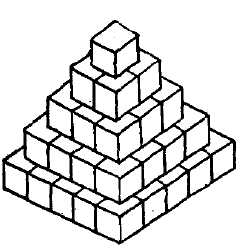
\includegraphics[scale=.7]{1.png}
\end{figure}

\begin{solution}
    显然,这一垛共有:$(1+4+9+16+25)$桶.
即:$1^2+2^2+3^2+4^2+5^2=55$桶.

这就是说,前五个自然数的平方
和等于55.

一般地,如果由前n个自然数的
平方组成的数列$1^2,2^2,3^2,\ldots,n^2$.
如何求出它们的和呢?能不能导出一
个通用的公式呢?

以下我们将先对这个数列的前$n$项和的特点进行
分析,然后应用待定系数法导出它的求和公式.

设$1^2+2^2+\cdots+n^2=S(n)$,在$S(n)$中,$n$代表项数.显然有:
\[\begin{split}
   S(0)&=0\\ S(1)&=1\\ S(2)&=1^2+2^2=5\\ S(3)&=1^2+2^2+3^2=14\\
   \cdots \cdots&\cdots\cdots\\ 
   S(n)&=1^2+2^2+\cdots+n^2\\ 
   S(n+1)&=1^2+2^2+\cdots+n^2+(n+1)^2 
\end{split}\]

而且还可以看出:无论项数$n$取几,总有
\[S(n+1)-S(n)=(n+1)^2=n^2+2n+1\]
可见,$S(n)$很可能是一个关于项数$n$的多项式,
它只要满足两个性质:
\begin{enumerate}
    \item $S(0)=0$
    \item $S(n+1)-S(n)=n^2+2n+1$ ($n$的二次式)
\end{enumerate}
\end{solution}

这就启示我们,如果能求出一个多项式$S(x)$, 能
满足以上两条性质,即$S(0)=0$, $S(x+1)-S(x)$是
一个二次式.那么,所求数列的前$n$项和,就是当$x
=n$时,多项式$S(x)$的值$S(n)$.

但是,满足以上两条性质的多项式$S(x)$应该是
几次多项式呢?

我们不妨设$S(x)$是$m$次多项式,即
\[S(x)=ax^m+bx^{m-1}+\cdots+cx+d\quad (a\ne 0)\]
则:$S(x+1)=a(x+1)x^m+b(x+1)x^{m-1}+\cdots+c(x+1)x+d$
由乘法公式,不难知道:
\[\begin{split}
    S(x+1)&= a(x^m+mx^{m-1}+\cdots +1)+b[x^{m-1}+(m-1)x^{m-2}+\cdots+1]\\
    +\cdots + c(x+1)+d\\
    &=ax^m+(b+am)x^{m-1}+\cdots +(c+\cdots)x+(a+b+\cdots +c+d)\\
\end{split}\]
$\therefore\quad S(x+1)-S(x)=(b+am-b)x^{m-1}+\cdots =amx^{m-1}+\cdots$

由于$am\ne 0$, 显然$S(x+1)-S(x)$是$m-1$次多
项式,因此,我们可以得出:

\begin{blk}{}
    当$S(x)$是一个$m$次多项式时,$S(x+1)-S(x)$必定是一个$m-1$次多项式.
\end{blk}

也就是说,多项式$S(x+1)-S(x)$的次数比多项
式$S(x)$的次数低一次.

这样,由于在我们以上所求问题中,$S(x+1)-S(x)$是二次多项式,所以,
\textbf{$S(x)$必定是一个三次多项式}.

基于以上分析,以下我们就可以用待定系数法导
出前$n$个自然数平方的求和公式.


\begin{example}
    试求$1^2+2^2+\cdots+n^2$.
\end{example}


\begin{solution}
    设$1^2+2^2+\cdots+n^2=S(n)$

由分析知$S(n)$是一个关于项数$n$的三次式,
且 $S(0)=0$, $S(1)=1$, $S(2)=5$, $S(3)=14$.
其中,0是$S(n)$的一个根.

$\therefore\quad $由余式定理的推论,得:
\[S(n)=n(an^2+bn+c)\]
这里$a$、$b$、$c$都是待
定系数.

将$S(1)=1$, $S(2)=5$, $S(3)=14$分别代入上
式,即可得出
\[\begin{cases}
    1=a+6+c\\
5=2(4a+26+c)\\
14=3(9a+36+c)
\end{cases}\Rightarrow\quad \begin{cases}
    a+b+c=1\\
4a+2b+c=\frac{5}{2}\\
9a+3b+c=\frac{14}{3}
\end{cases}\]
解这个方程组,得$a=\frac{1}{3},\quad b=\frac{1}{2},\quad c=\frac{1}{6}$
因此:
\[\begin{split}
    S(n)&=n\left(\frac{1}{3}n^2+\frac{1}{2}n+\frac{1}{6}\right)\\
&=\frac{n}{6}(2n^2+3n+1)\\
&=\frac{1}{6}n(n+1)(2n+1)
\end{split}\]
\end{solution}


\begin{ex}
    试用待定系数法求$1^3+2^3+\cdots+n^3$.
\end{ex}



\section*{习题7.2}
\addcontentsline{toc}{subsection}{习题7.2}
\begin{enumerate}
    \item 已知$x^4+4x^3+6px^2+4qx+r$能被$x^3+3x^2+9x+3$整
    除,试求$p$、$q$、$r$的值.
    \item 已知$f(x)=ax^2+bx+c$是一个完全平方式,试用待定
    系数法证明:$b^2-4ac=0$.
    \item 试用待定系数法把$f(x)=3x^3-10x^2+13$表示成$(x-2)$
    的各次方幂和.
    \item 用待定系数法,把$x^4-2x^2-2$表示成$x^2-x+1$的各
    次方幂和.
    \item 已知$x^3-x^2-8x+12=0$有两个根相等,试解这个方
    程.
    \item 已知方程$x^3-4x^2+x+k=0$有一个根是$-1$, 试求
    它的另外两个根.
    \item  如果方程$x^3+px^2+qx+r=0$有两个根互为相反数,
    试求$p,q,r$应具有什么关系?
    \item  化下列各分式为部分分式
    \begin{multicols}{2}
  \begin{enumerate}
\item  $\frac{3 x-4}{x^{2}-3 x+2}$
\item  $\frac{x^{2}+x-3}{(x-1)(x-2)(x-3)}$
\item $\frac{x^{2}-2}{x^{3}-3 x^{2}+2 x}$
\item  $\frac{x^{3}-6 x^{2}+4 x+8}{(x-3)^{4}}$
\item  $\frac{2 x^{2}+1}{x^{3}-1}$
\item  $\frac{21 x-14}{(x-3)^{2}(2 x+1)}$
\item  $\frac{8 x}{(x+1)\left(x^{2}-1\right)}$
\item  $\frac{x^{2}+x+1}{\left(x^{2}+1\right)\left(x^{2}+2\right)}$
\end{enumerate}      
    \end{multicols}

\item 求下列各算术平方根:
\begin{multicols}{2}
   \begin{enumerate}
    \item  $\sqrt{5+2 \sqrt{6}}$
    \item  $\sqrt{15-2 \sqrt{56}}$
    \item  $\sqrt{11+4 \sqrt{7}}$
    \item  $\sqrt{26-8 \sqrt{10}}$  
\end{enumerate}     
\end{multicols}

\item 求下列数列的前 $n$ 项和:
    $1^{4}, 2^{4}, 3^{4}, \ldots , n^{4}, \ldots$

\end{enumerate}






\section*{本章内容要点}

本章的主要内容是两种常见数列的求和及待定系数法与它的应用.

一、等差数列

\begin{enumerate}
    \item 按顺序排好的一列数中,如果从第二个数
起,每一个数与它前一个数的差都相等,那么,这一列数叫做等差数列.

设等差数列的首项为$a_1$, 公差为$d$, 项数为$n$, 末项为$a_n$及前$n$项和为$S_n$, 则有以下关系式:
\[\begin{split}
    a_n&=a_1+(n-1)d\\
    S_n&=\frac{n}{2}[2a_1+(n-1)d]=\frac{n}{2}(a_1+a_n)
\end{split}\]

如果已知$a_1,a_n,n,d,S_n$中的任意三个,就可以利用这两个公式,求出另两个.

\item 在两个已知数$a,b$之间,插入$n$个数构成等
差数列的问题,实际上就是已知首项$a$, 末项$b$及项数$n+2$, 要求出公差,进而可以求出插入的各项,还可以求出所有项的和.
\end{enumerate}

\vskip 2ex 
二、等比数列

按顺序排好的一列数中,如果从第二个数起,每一个数与它前一个数的比都相等,那么,这一列数叫
做等比数列.

设等比数列的首项为$a_1$, 公比为$q$, 项数为$n$, 末项为$a_n$, 前$n$项的和为$S_n$, 则有以下关系式:
\[\begin{split}
    a_n&=a_1q^{n-1}\\
    S_n&=\frac{a_1(1-q^n)}{1-q}
\end{split}\]

公比$q$的取值,决定了等比数列各项的大小变化趋向:如果首项$a_1>0$(或$<0$),那么,
\begin{itemize}
    \item 当$q>1$时,等比数列逐项增大(或减小);
    \item 当$0<q<1$时,等比数列逐项减小(或增大);
    \item 当$q<0$时,等比数列各项将正、负相间,逐项在正、负值之间摆动.
\end{itemize}

\vskip 2ex 
三、待定系数法是一个重要的数学方法,其根据就是多项式恒等的性质.其方法的要点就是:引进未定系数,列出恒等式并进而得出含有未定系数的方程组,求出未定系数.

待定系数法应用广泛,具体作法中又有一定的技巧,除可以求商式、余式、分解因式、寻求方程的根与系数间的关系外,还应从以下应用中进一步去掌握:
\begin{itemize}
    \item 求多项式与解方程;
    \item    用一个较低次的多项式的各次幂,表示另一个多项式;
    \item     将分式化成部分分式;
    \item 求形如$a\pm 2\sqrt{b}$的数的算术平方根;
    \item 求数列$1^b,\; 2^b,\; 3^b, \ldots,n^b,\ldots$ 前$n$项和($b$是大于1的一个自然数).
\end{itemize}


\section*{复习题七}
\addcontentsline{toc}{section}{复习题七}

\begin{enumerate}
    \item 求下列数列的前 10 项和及第$n$项.
\begin{enumerate}
    \item $0,\;-2,\;-4,\;-6, \ldots$;
    \item $\frac{1}{2},\;-\frac{1}{4},\; \frac{1}{8},\;-\frac{1}{16}, \ldots$;
    \item $-0.1,\;0.1,\;0.3,\;0.5 \ldots$;
    \item $9,\;3,\;1,\; \frac{1}{3},\; \frac{1}{9} \ldots$.
\end{enumerate}

\item 试求出下列数列的第 $n$ 项, 并导出它的前 $n$ 项求和公式:
\begin{enumerate}
    \item $1 \frac{1}{2},\; 2 \frac{1}{4}, \;3 \frac{1}{8} ,\; 4 \frac{1}{16}, \ldots$;
    \item $ 1.3,1.03,1.003,1.0003, \ldots$;
    \item $\frac{1}{1 \times 2},\; \frac{1}{2 \times 3},\; \frac{1}{3 \times 4},\; \frac{1}{4 \times 5},\ldots$.
\end{enumerate}

\item 如果有三个数成等差数列, 又成等比数列, 那么, 你能
    说明这三个数一定相等吗?
    \item 首项为100,公差为$-10$的等差数列中,前多少项的和最大?求出这个和.
\item  如果 $a, b, c$ 分别是一等比数列的第 $p, q, r$ 项, 试说
    明:
    $$a^{q-r} \cdot b^{r-p} \cdot c^{p-q}=1$$
    
    提示:设这一数列的公比为 $t$, 并将$a$视为首项, 则 $b, c$分别是第$q-p+1$、$r-p+1$项.

\item 求和:$S_n=\frac{1}{2}+\frac{2}{2^2}+\frac{3}{2^3}+\frac{4}{2^4}+\cdots+\frac{n}{2^n}$

提示:可以先求$S_n-\frac{1}{2}S_n$


\item 已知$f(-1)=0,\; -5f(0)=-\frac{10}{3}f(-2)=f(-3)=-20$,试求:$f\left(-\frac{1}{2}\right)$及$f\left(-\frac{5}{2}\right)$的值.

\item $\ell$和$m$是何值时,方程$\poly{1,4,-2,\ell ,m}=0$能有两组相等的根?
\item 方程$x^3+px^2+qx+r=0$要有两个根是互为相反数,试问:$p,q,r$必须符合什么条件?

\item 求和:
\[\frac{a}{x(x+a)}+\frac{a}{(x+a)(x+2a)}+\cdots +\frac{a}{[x+(n-1)a](x+na)}\]

提示:$\frac{a}{[x+(n-1)a](x+na)}=\frac{1}{x+(n-1)a}-\frac{1}{x+na}$

\item 将分式 $\frac{\poly{6,5,0,-7}}{\poly{3,-2,-1}}$ 化成部分分式.

\item 证明:如果$a,b,c$成等比数列,那么方程
\[(a^2+b^2)x^2-2b(a+c)x+b^2+c^2=0\]
有两个相等的实数根,且这个实数根正好等于公比.

提示:$a,b,c$之间有关系$b^2=ac$

\end{enumerate}



\end{document}